% !TEX program = xelatex
\documentclass[a4paper,11pt,openany]{memoir}
\usepackage{amsmath}
%\usepackage[sc,osf]{mathpazo}
%\usepackage[garamond]{mathdesign}
\usepackage{fontspec}
\usepackage[math-style=TeX]{unicode-math}
\usepackage{xunicode}
\usepackage{xltxtra}
\usepackage{polyglossia}
\defaultfontfeatures{Mapping=tex-text}
\setmainfont[   Path=fonts/xits/,
                BoldFont={xits-bold.otf},
                ItalicFont={xits-italic.otf},
                BoldItalicFont={xits-bolditalic.otf}
            ]{xits-regular.otf}
\setsansfont[   Path=fonts/frutiger/,
                Scale=MatchLowercase,
                BoldFont={FrutigerLTStd-Bold.otf},
                ItalicFont={FrutigerLTStd-Italic.otf},
                BoldItalicFont={FrutigerLTStd-BoldItalic.otf}
            ]{FrutigerLTStd-Roman.otf}
            
\setmathfont{xits-math.otf}
\setmathfont[version=roman,range=\mathcal,Path=fonts/]{latinmodern-math.otf}
%\setmathfont[range=\mathcal,Scale=MatchUppercase]{Lynda Cursive}
%\setmathfont[range=\mathup]{Garamond Premier Pro}
%\setmathfont[range=\mathit]{Garamond Premier Pro}
\setdefaultlanguage{danish}
\setotherlanguage[variant=british]{english}

\usepackage[usenames,dvipsnames,svgnames,table]{xcolor}
\usepackage{graphicx,epic,eepic}
\usepackage{tkz-graph,tkz-euclide}
\usetikzlibrary{calc,intersections,shapes.geometric,decorations.pathmorphing}
\usetikzlibrary{snakes,patterns,plotmarks,decorations.text}
\renewcommand*{\VertexSmallMinSize}{4pt}
\usepackage{tabulary}
\usepackage{pdfpages}
\usepackage{wrapfig}
\usepackage{pifont}
\usepackage{multirow}
\usepackage{colortbl}

%\renewcommand{\thefootnote}{\fnsymbol{footnote}}

\renewcommand\bibname{References}
\renewcommand{\(}{\begin{equation}}
\renewcommand{\)}{\end{equation}}
\newcommand{\vet}[1]{\underline{#1}}
\newcommand{\mtx}[1]{\underline{\underline{#1}}}
\newcommand{\ono}[1]{\frac{1}{#1}}
\newcommand{\half}{\frac{1}{2}}
\newcommand{\thehead}{}
\newcommand{\head}[1]{\renewcommand{\thehead}{#1}}
\newcommand{\theohead}{}
\newcommand{\ohead}[1]{\renewcommand{\theohead}{#1}}
\newcommand{\thetnote}{}
\newcommand{\tnote}[1]{\renewcommand{\thetnote}{#1}}
\newcommand{\bra}[1]{\left\langle #1 \right|}
\newcommand{\ket}[1]{\left| #1 \right\rangle}
\newcommand{\braket}[2]{\left\langle#1\middle|#2\right\rangle}
\newcommand{\obraket}[3]{\left\langle#1\middle|#2\middle|#3\right\rangle}
\newcommand{\emf}{\mathcal{E}}
\newcommand{\di}{\text{d}}

\newenvironment{infilsf}{
    \begin{sffamily}
    \setmathfont[range=\mathup/{num},
                 Scale=MatchLowercase,
                 Path=fonts/frutiger/,
                 ]{FrutigerLTStd-Roman.otf}
    \setmathfont[range=\mathit/{latin,Latin},
                 Scale=MatchLowercase,
                 Path=fonts/frutiger/,
                    ]{FrutigerLTStd-Italic.otf}
    \setmathfont[range=\mathit/{greek,Greek},
                 Scale=MatchLowercase,
                 Path=fonts/dejavu/,
                    ]{DejaVuSans-Oblique.ttf}
    \setmathfont[range=\mathup/{greek,Greek},
                 Scale=MatchLowercase,
                 Path=fonts/dejavu/,
                    ]{DejaVuSans.ttf}
%    \setmathfont[range=\text,
%                 Scale=MatchLowercase,
%                 Path=fonts/frutiger/,
%                    ]{FrutigerLTStd-Roman.otf}
}{
    \setmathfont{xits-math.otf}
    \setmathfont[range=\mathcal,Path=fonts/]{latinmodern-math.otf}
    \end{sffamily}
}

\newenvironment{new}{\color{Blue}}{}

\definecolor{kugray}{RGB}{102,102,102}
\definecolor{kugray1}{RGB}{52,52,52}
\definecolor{natgreen}{RGB}{50,93,61}
\definecolor{natgreen1}{RGB}{105,146,115}
\definecolor{natgreen2}{RGB}{161,168,171}
\definecolor{natcomp}{RGB}{93,50,82}
\definecolor{natcomp1}{RGB}{172,99,154}
\definecolor{natcomp2}{RGB}{195,154,186}
\definecolor{natlcomp}{HTML}{5d323d}
\definecolor{natrcomp}{HTML}{52325d}
\definecolor{natyellow}{HTML}{5d3d32}
\definecolor{natblue}{HTML}{32525d}

\makepagestyle{fancy}

\makepsmarks{fancy}{%
\nouppercaseheads
\createmark{chapter}{left}{nonumber}{}{}
\createmark{section}{right}{shownumber}{}{ \space}
\createplainmark{toc}{both}{\contentsname}
\createplainmark{lof}{both}{\listfigurename}
\createplainmark{lot}{both}{\listtablename}
\createplainmark{bib}{both}{\bibname}
\createplainmark{index}{both}{\indexname}
\createplainmark{glossary}{both}{\glossaryname}}

\makeoddhead{fancy}
   {}{}{}
\makeoddfoot{fancy}{\makebox[0pt][r]{\raisebox{15pt}[20pt]{\textcolor{natgreen}{\rule{1.1\spinemargin}{1pt}}}\makebox[0pt][l]{\raisebox{15pt}[20pt]{\textcolor{natgreen}{\rule{\paperwidth}{1pt}}}}}\textcolor{kugray}{\textsf{\rightmark}}}{}{\textcolor{kugray}{\textsf{\thepage}}}
\makeevenfoot{fancy}{\textcolor{kugray}{\textsf{\thepage}}}{}{\textcolor{kugray}{\textsf{\leftmark}}\makebox[0pt][l]{\raisebox{15pt}{\textcolor{natgreen}{\rule{1.1\spinemargin}{1pt}}}}\makebox[0pt][r]{\raisebox{15pt}{\textcolor{natgreen}{\rule{\paperwidth}{1pt}}}}}
\setlength{\footskip}{40pt}
\pagestyle{fancy}
\aliaspagestyle{chapter}{fancy}

\captionnamefont{\sffamily\color{natgreen}\bfseries} \captiontitlefont{\footnotesize} \captionstyle{\\}
\renewcommand*{\printchaptername}{}
\renewcommand*{\chapternamenum}{}
\renewcommand*{\afterchapternum}{}
\renewcommand{\chapnumfont}{\chaptitlefont\sffamily\HUGE}
\renewcommand{\printchapternum}{\chapnumfont \colorbox{natgreen}{\textcolor{white}{\hspace{.2em}\thechapter\hspace{.2em}}}\hspace{1em}}
\setsecheadstyle{\large\bfseries}
\setsubsecheadstyle{\bfseries}
\setsubsubsecheadstyle{}
\setsecnumformat{\textsf{\color{natgreen}\csname the#1\endcsname\quad}}
\maxsecnumdepth{subsubsection}
\renewcommand{\labelenumi}{\sffamily\bfseries\color{natgreen}\theenumi.}
\renewcommand{\labelitemi}{\color{natgreen}\ding{110}}
\renewcommand{\labelitemii}{\color{natgreen}\textbullet}
\setcounter{tocdepth}{2}

\setlength{\arrayrulewidth}{2pt}

\newsubfloat{figure}

\hyphenation{be-stem-mes}
\hyphenation{rest-klas-se-sæt-ning}
\hyphenation{Ham-il-ton}
\hyphenation{ATLAS}
\hyphenation{Atlas}
\hyphenation{CERN}
\hyphenation{i-den-ti-cal}
\hyphenation{pro-vid-ed}
\hyphenation{Calc-HEP}
\usepackage[pdfusetitle]{hyperref}
\urlstyle{sf}


\begin{document}
\begin{english}
\begin{titlingpage}
{
\definecolor{kugray}{RGB}{102,102,102}
\definecolor{natgreen}{RGB}{50,93,61}
\thispagestyle{empty}
\newlength{\topma}\setlength{\topma}{-1in}\addtolength{\topma}{-\headsep}\addtolength{\topma}{-\voffset}\addtolength{\topma}{11mm}
\newlength{\sidema}\setlength{\sidema}{-1in}\addtolength{\sidema}{-\hoffset}\addtolength{\sidema}{-\oddsidemargin}\addtolength{\sidema}{-\marginparsep}\addtolength{\sidema}{15mm}
\newlength{\textwa}\setlength{\textwa}{\paperwidth}\addtolength{\textwa}{-35mm}\addtolength{\textwa}{-\textwidth}
\newlength{\textha}\setlength{\textha}{-\textheight}\addtolength{\textha}{\paperheight}\addtolength{\textha}{-11mm}\addtolength{\textha}{-.1\paperheight}
\changepage{\textha}{\textwa}{}{\sidema}{}{-\topmargin}{-\headheight}{\topma}{}
%\setlength{\parindent}{0pt}
\noindent\begin{minipage}[t]{.8\textwidth}
\noindent\raggedright \textcolor{kugray}{\fontspec[Path=fonts/garamond/]{GaramondPremrPro.otf}\addfontfeature{LetterSpace=13.0}\fontsize{17}{17}\selectfont\textsc{niels bohr institute}}

\vspace{.2em}\textcolor{kugray}{\fontspec[Path=fonts/garamond/]{GaramondPremrPro.otf}\addfontfeature{LetterSpace=13.0}\fontsize{14}{17}\selectfont\textsc{university of copenhagen}}
\end{minipage}\hfill\begin{minipage}[t]{32mm}\raggedleft \vspace{16mm} 
\includegraphics[height=44mm]{KUnat.pdf}
\end{minipage}


\newlength{\markbump}\setlength{\markbump}{.3\paperwidth}\addtolength{\markbump}{-11mm}
\newlength{\markdown}\setlength{\markdown}{-75mm}\addtolength{\markdown}{0em}\addtolength{\markdown}{\paperheight}\addtolength{\markdown}{.15\paperwidth}
\noindent\makebox[0pt][l]{\hspace{\markbump}\raisebox{-\markdown}[0pt][0pt]{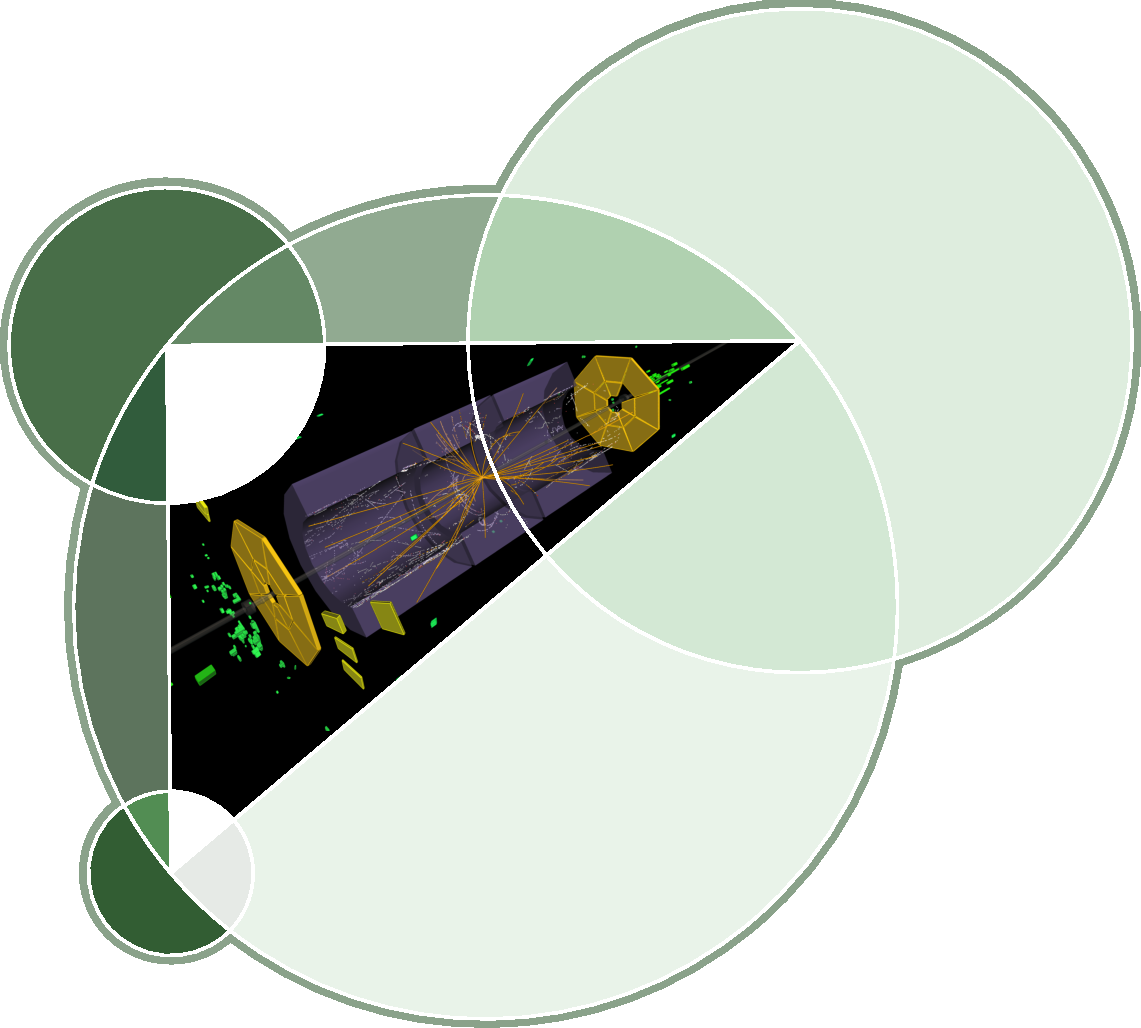
\includegraphics[height=.9\paperwidth]{atlaskugrid.pdf}}}\makebox[0pt][r]{\raisebox{3.2mm}[0pt][0pt]{\textcolor{natgreen}{\rule{.06\paperwidth}{.7pt}}}}\makebox[0pt][l]{\raisebox{3.2mm}[0pt][0pt]{\textcolor{natgreen}{\rule{.95\paperwidth}{.7pt}}}}





\bigskip

{\sffamily
{\textbf{ }

\vspace{2em}}

{\huge \textbf{Master's thesis}

\vspace{.3em}}

{\Large Kristoffer Levin Hansen}

\vspace{3em}

{\Huge Searching for {\fontspec[Path=fonts/dejavu/,Scale=MatchLowercase,BoldItalicFont={DejaVuSansCondensed-BoldOblique.ttf},BoldFont=DejaVuSansCondensed-Bold.ttf,ItalicFont=DejaVuSans-Oblique.ttf]{DejaVuSansCondensed.ttf}\textit{γγ}} contact interactions with 

the ATLAS detector at the LHC}
\vspace{7em}

{\Large Academic advisor: Jørgen Beck Hansen}
\vfill

\today}
\clearpage}
\thispagestyle{empty}
  \phantom{p}
\vspace{1.16\textwidth}

\begin{center}
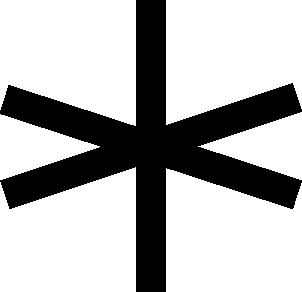
\includegraphics[width=.1\textwidth]{star1}
\end{center}
\clearpage
\end{titlingpage}
\frontmatter

\tableofcontents
\mainmatter

\chapter{Introduction}

Since the late 1960s, our---at times evolving---understanding of the properties and interactions of the fundamental particles has been summarised by the Standard Model. An overview of a selection of these properties and interactions is given in fig.~\ref{SMsum}.

\begin{figure}[hbt]
\begin{minipage}[b]{.74\textwidth}
\begin{infilsf}
\begin{sffamily}\begin{scriptsize}
\pgfdeclarelayer{back}
\pgfsetlayers{back,main}
\begin{tikzpicture}[yscale=1.8,xscale=0.35]

\tikzstyle{quark}=[font=\footnotesize,white,circle,draw=white,fill=natgreen,inner sep=0pt,minimum size=12pt]
\tikzstyle{gauge}=[font=\footnotesize,white,circle,draw=white,fill=natcomp,inner sep=0pt,minimum size=12pt]
\tikzstyle{higgs}=[font=\footnotesize,white,circle,draw=white,fill=natyellow,inner sep=0pt,minimum size=12pt]
\tikzstyle{lepton}=[font=\footnotesize,white,circle,draw=white,fill=natblue,inner sep=0pt,minimum size=12pt]
\tikzstyle{quarko}=[fill=white,circle,draw=natgreen,inner sep=0pt,minimum size=16pt]
\tikzstyle{gaugeo}=[fill=white,circle,draw=natcomp,inner sep=0pt,minimum size=16pt]
\tikzstyle{higgso}=[fill=white,circle,draw=natyellow,inner sep=0pt,minimum size=16pt]
\tikzstyle{leptono}=[fill=white,circle,draw=natblue,inner sep=0pt,minimum size=16pt]
\tikzstyle{inter}=[kugray!50, ultra thick,cap=rect]
\tikzstyle{under}=[line width=3pt,white]

\draw (-3.5,1.8) -- (-3.5,-1.5) -- (-1.7,-1.5) [snake=zigzag] -- (-.3,-1.5) [snake=none] --  (21,-1.5) -- (21,1.8) -- cycle;
\draw (-3.5,0) node[left] {0} -- +(8pt,0);
\draw (-3.5,1) node[left] {1} -- +(8pt,0);
\draw (-3.5,-1) node[left] {-1} -- +(8pt,0);
\draw (-2,-1.5) -- +(0,2.5pt) +(0,-.9em) node[above] {0};
\foreach \x in {0,1}
\draw (\x*2.303,-1.5) -- +(0,2.5pt) 
    +(0.693,0) -- +(0.693,1.5pt) +(1.1,0) -- +(1.1,1.5pt) 
    +(1.39,0) -- +(1.39,1.5pt) +(1.61,0) -- +(1.61,1.5pt) +(1.79,0) -- +(1.79,1.5pt)
    +(1.95,0) -- +(1.95,1.5pt) +(2.08,0) -- +(2.08,1.5pt) +(2.2,0) -- +(2.2,1.5pt);
\foreach \x in {2,3,...,8}
\draw (\x*2.303,-1.5) -- +(0,2.5pt) +(0,-.9em) node[above] {$10^{\x}$}
    +(0.693,0) -- +(0.693,1.5pt) +(1.1,0) -- +(1.1,1.5pt) 
    +(1.39,0) -- +(1.39,1.5pt) +(1.61,0) -- +(1.61,1.5pt) +(1.79,0) -- +(1.79,1.5pt)
    +(1.95,0) -- +(1.95,1.5pt) +(2.08,0) -- +(2.08,1.5pt) +(2.2,0) -- +(2.2,1.5pt);
\draw (0,-1.5) -- +(0,2.5pt) +(0,-.9em) node[above] {1};
\draw (2.303,-1.5) -- +(0,2.5pt) +(0,-.9em) node[above] {10};
\draw (9*2.303,-1.5) -- +(0,2.5pt) +(0,-.9em) node[above] {$10^9$};
\node at (-4.8,1.7) [rotate=90,left] {Electromagnetic charge [e]};
\node at (21,-1.8) [left] {Mass [eV/c$^2$]};
\draw (7.74,0.667) node [quarko] (u) {} node {\tikz {\fill[natgreen] (0,0) -- ++(0,8pt) arc (90:-90:8pt) -- cycle; \draw +(180:8pt);}} node [quark] {u};
\draw (8.48,-0.333) node [quarko] (d) {} node {\tikz {\fill[natgreen] (0,0) -- ++(0,8pt) arc (90:-90:8pt) -- cycle; \draw +(180:8pt);}} node [quark] {d};
\draw (14.06,0.667) node [quarko] (s) {} node {\tikz {\fill[natgreen] (0,0) -- ++(0,8pt) arc (90:-90:8pt) -- cycle; \draw +(180:8pt);}} node [quark] {s};
\draw (11.46,-0.333) node [quarko] (c) {} node {\tikz {\fill[natgreen] (0,0) -- ++(0,8pt) arc (90:-90:8pt) -- cycle; \draw +(180:8pt);}} node [quark] {c};
\draw (18.97,0.667) node [quarko] (t) {} node {\tikz {\fill[natgreen] (0,0) -- ++(0,8pt) arc (90:-90:8pt) -- cycle; \draw +(180:8pt);}} node [quark] {t};
\draw (15.25,-0.333) node [quarko] (b) {} node {\tikz {\fill[natgreen] (0,0) -- ++(0,8pt) arc (90:-90:8pt) -- cycle; \draw +(180:8pt);}} node [quark] {b};
\draw (-2,0) ++(100:6.5pt) ++(-4.47pt,0) node (gamma) [gaugeo] {} node {\tikz {\shade[top color=white,bottom color=natcomp] (0,0)  +(-80:12pt) -- +(-45:8pt) arc (-45:-115:8pt) -- cycle; \filldraw[natcomp] (0,0) circle (8pt); \draw +(100:12pt);}} node [gauge] {$\gamma$};
\draw (-2,0) ++(-80:6.5pt) ++(4.47pt,0) node [gaugeo] (g) {} node {\tikz {\shade[top color=natcomp,bottom color=white] +(100:12pt) -- +(135:8pt) arc (135:65:8pt) -- cycle; \filldraw[natcomp] (0,0) circle (8pt); \draw +(-80:12pt);}} node [gauge] {g};
\draw (-2,0) node {\tikz \fill[natcomp] circle (1pt);};
\draw (18.33,0) ++(100:6.5pt) ++(-4.47pt,0) node [gaugeo] (Z) {} node {\tikz {\shade[top color=white,bottom color=natcomp] (0,0)  +(-80:12pt) -- +(-45:8pt) arc (-45:-115:8pt) -- cycle; \filldraw[natcomp] (0,0) circle (8pt); \draw +(100:12pt);}} node [gauge] {Z};
\draw (18.20,1) node [gaugeo] (W+) {} node {\tikz {\filldraw[natcomp] (0,0) circle (8pt);}} node [gauge] {\tiny W$^+$};
\draw (18.20,-1) node [gaugeo] (W-) {} node {\tikz {\filldraw[natcomp] (0,0) circle (8pt);}} node [gauge] {\tiny W$^-$};
\draw (18.65,0)  ++(-80:6.5pt) ++(4.47pt,0) node [higgso] (H) {} node {\tikz {\shade[top color=natyellow,bottom color=white] +(100:12pt) -- +(135:8pt) arc (135:65:8pt) -- cycle; \draw +(-80:12pt); \draw[natyellow] (0,0) circle (8pt);}} node [higgs] {H};
\draw (18.33,0) node {\tikz \fill[natcomp] circle (1pt);};
\draw (18.65,0) node {\tikz \fill[natyellow] circle (1pt);};
\draw (0.79,0) node [leptono] (ve) {} node {\tikz {\fill[natblue] (0,0) -- ++(0,8pt) arc (90:-90:8pt) -- cycle; \draw +(180:8pt);}} node [lepton] {$\nu_{\text e}$};
\draw (5.14,0) node [leptono] (vmu) {} node {\tikz {\fill[natblue] (0,0) -- ++(0,8pt) arc (90:-90:8pt) -- cycle; \draw +(180:8pt);}} node [lepton] {$\nu_\mu$};
\draw (9.65,0) node [leptono] (vtau) {} node {\tikz {\fill[natblue] (0,0) -- ++(0,8pt) arc (90:-90:8pt) -- cycle; \draw +(180:8pt);}} node [lepton] {$\nu_\tau$};
\draw (6.24,-1) node [leptono] (e) {} node {\tikz {\fill[natblue] (0,0) -- ++(0,8pt) arc (90:-90:8pt) -- cycle; \draw +(180:8pt);}} node [lepton] {e};
\draw (11.57,-1) node [leptono] (mu) {} node {\tikz {\fill[natblue] (0,0) -- ++(0,8pt) arc (90:-90:8pt) -- cycle; \draw +(180:8pt);}} node [lepton] {$\mu$};
\draw (14.39,-1) node [leptono] (tau) {} node {\tikz {\fill[natblue] (0,0) -- ++(0,8pt) arc (90:-90:8pt) -- cycle; \draw +(180:8pt);}} node [lepton] {$\tau$};

\begin{pgfonlayer}{back}
\node at (12,1) [inner sep=0] (uqs) {};
\node at (20.7,.6) [inner sep=0] (qgnode) {};
\draw [inter] (u) to[out=0,in=270,max distance=7pt]  (uqs);
\draw [inter] (s) to[out=170,in=270,max distance=4pt] (uqs);
\draw [inter] (t) to[out=190,in=270,max distance=25pt] (uqs);
\draw [inter] (d) to[out=5,in=270,max distance=30pt] (uqs);
\draw [inter] (c) to[out=60,in=270,max distance=10pt] (uqs);
\draw [inter] (b) to[out=170,in=270,max distance=20pt] (uqs)
                  to[out=90,in=40,max distance=17pt] (g);
\draw (g) node[below right] {\tikz {\draw [inter] (0,0) to[in=-40,out=-90,min distance=20pt] (0,0);}};
\draw [inter] (uqs) to[out=90,in=30,max distance=15pt] (gamma);
\draw [inter] (uqs) to[out=90,in=150,max distance=7pt] (W+);
\draw [inter] (uqs) .. controls (12,1.4) and (20.7,1.7) .. (qgnode.south)
                    to[out=270,in=10,max distance=7pt] (Z);
\draw [inter] (qgnode) to[out=270,in=20,max distance=10pt] (H);
\draw [inter] (qgnode) to[out=270,in=20,max distance=30pt] (W-);

\draw [under] (gamma) -- ++(15,0) node [inner sep=0] (gamw) {};
\draw [under] (gamw.west) to[out=0,in=90,max distance=30pt] (W-);
\draw [under] (gamw.west) to[out=0,in=250,max distance=20pt] (W+);
\draw [inter] (gamma) -- (gamw.east);
\draw [inter] (gamw.west) to[out=0,in=250,max distance=20pt] (W+);
\draw [inter] (gamw.west) to[out=0,in=90,max distance=30pt] (W-);

\node at (17,-.3) [inner sep=0] (wz-) {};
\node at (17,.6) [inner sep=0] (wz+) {};
\draw [under] (wz-) -- (wz+) to[out=270,in=160,max distance=10pt] (Z);
\draw [under] (H) to[out=30,in=-5,min distance=30pt] (W+);
\draw [inter] (W-) to[out=160,in=270,max distance=10pt] (wz-)
           to (wz+.north) to[out=90,in=200,max distance=10pt] (W+);
\node [above right] at (W+) {\tikz {
    \draw[under] (0,0) to[out=40,in=90,min distance=20pt] (0,0);
    \draw[inter] (0,0) to[out=40,in=90,min distance=20pt] (0,0);}};
\draw [inter] (wz-) to[out=90,in=200,max distance=10pt] (Z);
\draw [inter] (wz+) to[out=270,in=160,max distance=10pt] (Z);
\draw [inter] (W-) -- (H);
\draw (W-) node[below right] {\tikz {\draw [inter] (0,0) to[in=-40,out=-90,min distance=20pt] (0,0);}};
\draw [inter] (H) to[out=50,in=-10,max distance=5pt] (Z);
\draw [inter] (H) to[out=30,in=-5,min distance=30pt] (W+);

\draw (tau) ++(1.5,.25) node [inner sep=0] (lepga) {};
\draw [inter] (tau) to[out=70,in=180,max distance=3pt] (lepga)
                    to[out=0,in=270,max distance=10pt] (wz-);
\draw [inter] (mu) to[out=70,in=180,max distance=3pt] ++(1.5,.25) -- (lepga);
\draw [inter] (e) to[out=70,in=180,max distance=3pt] ++(1.5,.25)
              node [inner sep=0] (ega) {} -- (lepga);
\draw [inter] (lepga) to[out=0,in=152,max distance=10pt] (W-);

\draw (vmu) ++(-1.5,-.25) node [inner sep=0] (neul) {};
\draw [inter] (vmu) to[out=250,in=0,max distance=3pt] (neul);
\draw [inter] (vtau) to[out=185,in=0,min distance = 30pt] (neul);
\draw [inter] (ve) -- ++(0,-.5) node [inner sep=0] (neud) {};
\draw [inter] (neul.east) to[out=180,in=90,max distance=7pt] (neud);
\draw [inter] (neud.north) to [out=270,in=180,max distance=10pt] (ega);

\draw (g) ++(-1,0) node [inner sep=0] (gamlep) {};
\draw [inter] (e) to [out=250,in=0,max distance=3pt] ++(-1.5,-.25)
              node (lepneu) [inner sep=0] {};
\draw [inter] (mu) to[out=250,in=0,max distance=3pt] ++(-1.5,-.25) -- (lepneu);
\draw [inter] (tau) to[out=250,in=0,max distance=3pt] ++(-1.5,-.25) -- (lepneu);
\draw [inter] (lepneu.east) to[out=180,in=270,max distance=20pt] (neud.north);
\draw [inter] (lepneu) to[out=180,in=270,max distance=30pt] (gamlep);
\draw [inter] (gamma) to[out=230,in=90] (gamlep.south);
\end{pgfonlayer}

\draw[inter,cap=round] (-2,1) -- (0,1) node[right,kugray] {Interactions};

\draw (-1,1.4) node [quarko] (n) {} node {\tikz {\fill[natgreen] (0,0) -- ++(0,8pt) arc (90:-90:8pt) -- cycle; \draw +(180:8pt);}} node [quark] {n};
\node at (n) {\tikz {\draw [white,postaction={decorate,decoration={text along path,text align=center,text={|\tiny|Spin}}}] ++(270:10pt) arc (270:90:10pt); \draw (-1,0) (1,0);}};
\begin{scope}
\clip (n.center) -- ++(2,0) -- ++(0,.2) -- ++(-2,0) -- cycle;
\draw (n) node [gaugeo] {} node {\tikz {\filldraw[natcomp] (0,0) circle (8pt);}} node [gauge] {n};
\end{scope}
\begin{scope}
\clip (n.center) -- ++(2,0) -- ++(0,-.2) -- ++(-2,0) -- cycle;
\draw (n) node [leptono] {} node {\tikz {\fill[natblue] (0,0) -- ++(0,8pt) arc (90:-90:8pt) -- cycle; \draw +(180:8pt);}} node [lepton] {n};
\end{scope}
\begin{scope}
\clip (n.center) -- ++(-2,0) -- ++(0,-.2) -- ++(2,0) -- cycle;
\draw (n) node [higgso] {} node {\tikz {\shade[top color=natyellow,bottom color=white] +(100:12pt) -- +(135:8pt) arc (135:65:8pt) -- cycle; \draw +(-80:12pt); \draw[natyellow] (0,0) circle (8pt);}} node [higgs] {n};
\end{scope}

\draw (n) ++(160:20pt) node [right,natgreen] {\tiny Quarks};
\draw (n) ++(-160:20pt) node [right,natyellow] {\tiny Higgs boson};
\draw (n) ++(0:20pt) node [above right,natcomp] {\tiny Gauge bosons};
\draw (n) ++(0:20pt) node [below right,natblue] {\tiny Leptons};

\end{tikzpicture}
\end{scriptsize}\end{sffamily}
\end{infilsf}
\end{minipage}
\hfill\begin{minipage}[b]{.25\textwidth}
\caption{An overview of the particles of the Standard Model. The particles are arranged by mass and charge. Colour indicates particle type, the filling of the border indicates the spin of particles and lines are drawn between those particles that the Standard Model describes interactions between. The currently known maximum bounds on neutrino masses have been used to place the neutrinos in the mass direction. Table values from \cite{wikism}.\label{SMsum}}
\end{minipage}
\end{figure}

In its current form, the Standard Model makes no attempt to explain any physics beyond this.\footnote{The overview in figure~\ref{SMsum} includes massive neutrinos, which have been found experimentally, even though the Standard Model does not at present include them. There are, however, several proposed methods of extending the SM to do so.} The most obvious missing element is gravity, which continues to resist grand unification. Other missing elements include a number of phenomena from cosmology, such as dark matter and dark energy, which may or may not be explained by particles or forces that a complete theory of fundamental particles and forces can be expected to include.

Within these limits, the Standard Model has been remarkably successful, withstanding decades of experimental tests, correctly predicting the existence and properties of a number of particles.\footnote{Most recently, the existence of the Higgs boson was confirmed experimentally. At the time of writing, confirmation of its predicted properties is still a work in progress.} Those successes not withstanding, there are some issues within the Standard Model.

As it is formulated, the SM depends on at least 19 numerical constants,\footnote{Not counting any additional constants needed to account for neutrino masses.} the value of which must be determined experimentally, since the model offers no insight into the origin of or relations between these constants. Worse still, as formulated in the SM, higher order corrections will tend to increase the Higgs mass, with no constraint save the Planck energy. This is one example of the hierarchy problem. The implication is that either some unknown physics exist between the Higgs mass scale and the Planck scale to constrain the Higgs mass, or the bare mass and couplings of the Higgs boson is very finely tuned to cancel the higher order contributions.

In the first case, we will obviously want to search for evidence of the unknown mechanism. In the latter case, we might expect there to be some underlying mechanism that ensures that the bare Higgs mass and the other free parameters of the SM have the proper value. Again, we will want to search for physics outside the SM, as a clue to what that underlying mechanism is.

There is also the possibility that neither of those mechanisms exist, since the Standard Model, strictly speaking, does not require them. In that case, searching for, and not finding any, new physics is still a valuable, albeit less illuminating, result.

In this thesis, we shall approach the task of searching for physics beyond the Standard Model by introducing to it an extension via the effective Lagrangian approach. Specifically, we will introduce a $q\bar q\rightarrow\gamma\gamma$ point interaction, and then simulating collision experiments with the new interaction at various strengths, to see how the outcome is affected. We can then, finally, compare the results of those pseudoexperiments to the results of actual collision experiments performed at CERN's Large Hadron Collider, and look for the same effects there.

\chapter{Theory}

While the detailed procedure for going from a general notion of expanding the Standard Model to creating a specific set of pseudoexperiments with which to compare experimental results are not part of the main thrust of this thesis, and will in any case be handled by various software tools in practice, what will follow is a brief overview of that process.

Since the new interaction will be introduced into the SM by the effective Lagrangian approach, the Lagrangian formulation of the Standard Model as a quantum field theory will be the starting point.

\section{The Lagrangian formulation of QFT}
In classical mechanics \cite{goldstein}, the Lagrangian formulation describes the path taken by a system between a given initial and final state---a particle with an initial and a final position, say---by finding the path that minimises the action $S$, which is defined as the integral along a given path over the Lagrangian $L$:
\[S[q]=\int_\textrm{path}dtL[q,\dot{q}],\]
where $q$ is a generalised coordinate. In this picture, the Lagrangian encapsulates the dynamics of the system. It is related to the Hamiltonian $H$ by
\(L = p\dot q- H,\label{htol}\)
where $p$ is momentum.

In quantum mechanics, the picture of a system travelling along a single, well-defined path from an initial to a final configuration no longer applies. In stead, a probability of going from an initial state $\ket{q}$ to a final state $\ket{q\prime}$ can be found as the absolute square of the transition amplitude\footnote{At this point, we should note that the common notation where $\hbar = c = 1$ will be used from this chapter onwards.} \cite{sred:tramp}
\[A=\bra{q\prime}e^{-i\hat H(t\prime-t)}\ket{q\phantom\prime},\]
where $\hat H$ is the Hamiltonian of the system. Since the idea of a singular path for the system was abandoned, in stead imagine the system travelling along each possible path simultaneously, each with its own transition amplitude. The total transition amplitude, then, is the sum of all the individual transition amplitudes. This can be connected to the classical case by supposing that, for a system with a classical limit, the transition amplitudes of paths close to the classical path will tend to amplify one another, while paths far from it will tend to cancel out.

Through some notational gymnastics, which involve carving the path integral into an infinite number of time steps, each integrated over every possible configuration, and imposing some conditions on the Lagrangian, it can be shown \cite{sred:tramp} that the expression above can be written as
\(A=\int\,\mathcal Dq\,\exp\left[i\int_t^{t^\prime}dt\,[p(t)\dot q(t)-H(p(t),q(t))]\right],\label{e.Dq}\)
where the integral is over all paths with position $q$ at time $t$ and position $q\prime$ at time $t\prime$. We recognise the expression in the innermost integral from eq.~\eqref{htol}.

For a local theory, it is possible to write the Lagrangian as a spatial integral over the Lagrangian density:
\[L=\int \,d^3x\,\mathcal L.\]
Thus, the action can be written as
\(S=\int\,d^4x\,\mathcal L,\label{e.S}\)
which, unlike the previous expression for $S$, is manifestly Lorenz invariant, so long as $\mathcal L$ is a Lorenz scalar. Given the ubiquity of local quantum field theories, it is common in quantum field theory to drop `density' from the name, and refer to $\mathcal L$ as the Lagrangian.

Finally, to get the field theory aspect, replace the generalised coordinate $q$ with a field configuration ``coordinate'' $\phi(x)$, which depends on the Lorenz vector $x$. In short, \eqref{e.Dq} can then be written as
\(A=\int\mathcal D\phi\, e^{iS[\phi]}.\label{e.Dphi}\)

As was the case in classical mechanics, the behaviour of a theory is fully described by its Lagrangian (density), and several models can be combined by adding together their respective Lagrangians. So it is that the Standard Model is described by the SM Lagrangian $\mathcal L_{SM}$, which can be considered as a sum of several, more specific, Lagrangians that describe the separate sectors of the SM. However, before we venture too deeply into the Standard Model, we shall first consider an alternate way of looking at the content of the Lagrangian.

\section{Feynman diagrams}
When studying individual processes described by a theory, Feynman diagrams are a useful tool. So useful, in fact, that much of the software developed to simulate processes is designed around them. To see how they work, consider the simple model described by the Lagrangian
\[\mathcal L= \half\partial^\mu\phi\partial_\mu\phi-\half m^2\phi^2-\frac{\lambda}{4!}\phi^4=\phi[\partial^2-m^2]\phi-\frac{\lambda}{4!}\phi^4\]
This is an example of a $\phi^4$ theory. The first terms in this Lagrangian, which involves two $\phi$s, describes a field propagating into another field, and the other one, which involves 4 $\phi$s, describes and interaction between four fields.

The goal will be to calculate the transition amplitude for a state $\ket{\phi_a}$ going to some other state $\ket{\phi_A}$. One procedure for doing so, which is inspired by \cite{wiki.feydiag}, is to start by writing the state as
\[\ket{\phi}=\int\frac{d^4k}{(2\pi)^4}\tilde\phi(k)\ket{k},\]
where $k$ is a four-momentum. Using eq.~\eqref{e.Dphi}, the transition amplitude can be expressed as
\(A\propto\int\frac{d^4k_A}{(2\pi)^4}\frac{d^4k_a}{(2\pi)^4}\int\mathcal D\phi\,\phi(k_A)\phi(k_a)e^{iS}.\label{transa}\)

To express $S$ in terms of momenta, we go back to the Lagrangian and express $\phi$ in terms of its Fourier modes:
\[\phi(x)=\int\frac{d^4k}{(2\pi)^4}e^{ikx}\tilde\phi(k)\]
The Lagrangian is now
\begin{align*}\mathcal L=&-\int\frac{d^4k}{(2\pi)^4}\frac{d^4k\prime}{(2\pi)^4} e^{i(k+k\prime)x}\tilde\phi(k)[kk\prime +m^2]\tilde\phi(k\prime)\\
&-\frac{\lambda}{4!}\int\frac{d^4p_1\,d^4p_2\,d^4p_3\,d^4p_4}{(2\pi)^{16}}e^{i(p_1+p_2+p_3+p_4)x}\tilde\phi(p_1)\tilde\phi(p_2)\tilde\phi(p_3)\tilde\phi(p_4).
\end{align*}
Inserting this into eq.~\eqref{e.S}, it becomes clear that $x$ only appears as a phase factor, which means that integrating over $x$ only produces delta functions:
\begin{align*}
S=&\int\frac{d^4k}{(2\pi)^4}\tilde\phi(-k)(k^2-m^2)\tilde\phi(k)\\
&-\frac{\lambda}{4!}\int\frac{d^4p_1\,d^4p_2\,d^4p_3\,d^4p_4}{(2\pi)^{16}}\tilde\phi(p_1)\tilde\phi(p_2)\tilde\phi(p_3)\tilde\phi(p_4)\delta(p_1+p_2+p_3+p_4),
\end{align*}
where, in the first term, the delta function identified $k\prime=-k$. The first term of the action describes the free part of the theory, and the second term describes the interacting part, so we will call them $S_F$ and $S_I$, respectively. Using this expression in place of $S$, we can Taylor expand in $\lambda$:
\[e^{iS}=e^{i(S_F+S_I)}=e^{iS_F}\left(1-iS_I+\frac{(-iS_I)^2}{2}+\frac{(-iS_I)^3}{3!}+\frac{(-iS_I)^4}{4!}+\cdots\right)\]
This assumes that $\lambda$ is small enough to make the interaction merely a pertubation of the theory.


Inserting this back into eq.~\eqref{transa}, we get an expression for the transition amplitude expanded in powers of $\lambda$. If we call these terms $A_n$, so that $A\propto\sum_{n=0}^\infty A_n$, the first term of the expansion is
\[A_0=\int\frac{d^4k_A}{(2\pi)^4}\frac{d^4k_a}{(2\pi)^4}\underbrace{\int\mathcal D\phi\,\phi(k_A)\phi(k_a)e^{iS_F}}_{D_0}.\]
Looking more closely at the part labelled $D_0$ above, we can expand it to find that
\[D_0=\int\mathcal D\phi\,\phi(k_A)\phi(k_a)e^{\int\frac{d^4k}{(2\pi)^4}\phi(k)[k^2-m^2]\phi(-k)},\]
which is a Gaussian (functional) integral \cite{armbjorn}:
\[\int d^nx\,x^k\cdots x^{2N}e^{-\half x^iA_{ij}x^j}.\label{gausint}\]
As such, the integral has the following solution, provided that the participating momenta are identical:
\[D_0=\half\frac{\delta^4(k_a-k_A)}{k^2-m^2}\int\mathcal D\phi\,e^{iS_F},\]
where the delta function is introduced to ensure that the momenta are identical, as required. Introducing this delta function is equivalent to imposing momentum conservation. The remaining integral over the free action corresponds to the vacuum $0\rightarrow0$ process in free theory, and is a constant with respect to $\phi$. This constant can be interpreted as the vacuum energy content of all space, which we will nevertheless simply divide out:
\[A\propto\int\frac{d^4k_A}{(2\pi)^4}\frac{d^4k_a}{(2\pi)^4}\,\frac{\int\mathcal D\phi\,\phi(k_A)\phi(k_a)e^{iS}}{\int\mathcal D\phi\,e^{iS_F}}\]
With this, we find that 
\[D_0=\frac{\delta^4(k_a-k_A)}{k^2-m^2},\]
which is the propagator in momentum space.


Were we to carry out the momentum integrations over $D_0$, there would evidently be a singularity at $k^2=m^2$. This singularity can be avoided by slightly modifying the integration path. There are several ways of doing this, including Feynman's prescription, which yields the expression $1/(k^2-m^2+i\epsilon)$, the Feynman propagator in momentum space. 


The second term in the expansion is
\[A_1=\int\frac{d^4k_A}{(2\pi)^4}\frac{d^4k_a}{(2\pi)^4}\left(\prod_{n=1}^4\frac{d^4p_n}{(2\pi)^4}\right)\,D_1,\]
where\footnote{Here, $\phi^n$ is shorthand for a product of $n$ $\tilde\phi$ functions of separate momenta.}
\[D_1=-\frac{i\lambda}{4!}\delta^4(p_1+p_2+p_3+p_4)\frac{\int\mathcal D\phi\,\phi^6e^{iS_F}}{\int\mathcal D\phi\,e^{iS_F}}.\] 
Solving the Gaussian integral tell us that $D_1$ is equal to a sum of terms of the form 
\(-\ono{3!2^3}\frac{i\lambda}{4!}\delta^4(p_1+p_2+p_3+p_4)\frac{\delta^4(k_1-p_1)}{{k_1}^2-m^2}\frac{\delta^4(p_2-p_3)}{{p_2}^2-m^2}\frac{\delta^4(p_4-k_A)}{{k_A}^2-m^2},\label{1t1f}\)
where the momenta are paired in all possible combinations. There are $6!$ different combinations, but they fall into only two groups of topologically inequivalent diagrams, as illustrated in figure~\ref{fey1t1o2}.


\begin{figure}[htb]
\begin{minipage}{.65\textwidth}
\begin{footnotesize}\begin{center}
\begin{tikzpicture}
\draw (-3,.2) node[left]{$a$} -- 
      ++(1,0) to[in=45,out=135,min distance=15mm,looseness=8] ++(0,0) --
      ++(1,0) node[right]{$A$};
\draw (1,.2) node[left]{$a$} -- ++(2,0) node[right]{$A$} 
      ++(-1,.5) to[in=45,out=-45,min distance=15mm,looseness=8] 
      ++(0,0) to[in=225,out=135,min distance=15mm,looseness=8] ++(0,0);
\end{tikzpicture}
\end{center}\end{footnotesize}
\end{minipage}
\hfill
\begin{minipage}{.3\textwidth}
\begin{center}\begin{footnotesize}
\begin{tikzpicture}
\draw (-1,0) node[left]{$a$} -- (1,0) node[right]{$A$};
\end{tikzpicture}
\end{footnotesize}\end{center}
\end{minipage}
\begin{minipage}[t]{.65\textwidth}
\caption{The two topologically inequivalent diagrams that can be constructed from the second term in the expansion of the $1\rightarrow1$ transition amplitude in eq.~\eqref{1t1f}. They are drawn by imagining the ingoing and outgoing states as labelled points, and drawing a line from one of these states to the state that its momentum is set equal to by the delta function in a propagator. The delta function over four momenta from the $\phi^4$ term is drawn as a vertex where exactly four lines come together.\label{fey1t1o2}
}
\end{minipage}
\hfill
\begin{minipage}[t]{.3\textwidth}
\caption{The first term drawn with the same method as fig.~\ref{fey1t1o2}.\label{fey1t1o1}}
\end{minipage}
\end{figure}


This way of illustrating the terms is called a Feynman diagram. The single, somewhat less complicated, Feynman diagram associated with the first term in the expansion is shown in fig.~\ref{fey1t1o1}.

By topologically inequivalent diagrams, we mean diagrams that cannot be rearranged to be identical with one another without disconnecting a line from a vertex\footnote{In the parlance of the topic, two topologies are inequivalent when there does not exist a continuous map that takes one into the other. However, to properly define all the terns in the previous sentence, we would need to venture beyond the scope of this thesis.}. In this context the ingoing and outgoing state labels are attached to the external lines. This becomes important when working with more in- and outgoing states and/or more vertices.

To count how may of each of the diagrams in fig.~\ref{fey1t1o2} there are, we note that there are $4!$ different ways of connecting lines to a vertex, each of the three lines can be drawn in both directions, giving a factor $2^3$, and the lines may be drawn in any order, giving a factor $3!$. These factors cancel out the factor $1/(3!2^3)$ from the solution of the Gaussian integral and the factor $1/4!$ from the $\phi^4$ term in the Lagrangian. Sadly, this way of counting diagrams doesn't give the correct number. In the left diagram, the factor 2 related to reversing the direction of the looping line counts diagrams that were already included in the $4!$ ways of connecting the vertex. In the right diagram, this is true for both of the looping lines, along with an additional factor 2 counting the order in which the looping lines are drawn, which was also already included in the factor $4!$ associated with the vertex, for a total overcounting of a factor $8$. These overcountings arise whenever there are symmetries in the diagrams, which allow us to reach the same diagram by two different manipulations. Note, though, that the symmetries that are responsible for these overcountings are apparent just by looking at it.

Looking at eq.~\eqref{1t1f}, one of the internal $p$ momenta can not be fixed to the external $k$ momenta, which leaves this term proportional to a diverging integral, associated with the looping line in the left diagram in fig.~\ref{fey1t1o2}. There are established methods for renormalising these divergent terms, however for the present purposes, we note simply that for any process, there will among the lowest order terms that describe it be a tree level\footnote{In graph theory, a tree is a connected, loop-free graph.} diagram, which is then the leading order diagram for that process. Because we are working in a pertubative regime by assumption, loop-level diagrams of that process will act as higher order corrections to that leading order term.

Knowing all this, it should be clear that enough information is available in a Feynman diagram to allow us to recover the terms in the expression for the transition amplitude that it represents. That being the case, it is possible to reverse the procedure by which we found the Feynman diagrams in the first place, and extract the expression for the transition amplitude from a set of Feynman diagrams. We can even start with constructing the Feynman diagrams, and recover the expression from them, thus bypassing the derivation above.


\begin{figure}[htb]
\hfill
\begin{tikzpicture}
\draw (-3,1) -- (-1,-1) (-3,-1) -- (-1,1);
\node[right] at (-1,0) {$=-i\lambda$};
\end{tikzpicture}
\hfill
\begin{tikzpicture}
\node[right] at (-1,0) {$=\dfrac{1}{k^2-m^2}$};
\draw (-3,0) -- (-1,0);
\node at (0,-1) {};
\node at (0,1) {};
\end{tikzpicture}
\hfill \phantom{d}
\caption{The building blocks for Feynman diagrams in $\phi^4$ theory. Once constructed, find the momentum of each propagator by imposing momentum conservation at each vertex. Any momentum that cannot be related to one of the external momenta is integrated over.
\label{phi4rules}}
\end{figure}


The rules for constructing the Feynman diagrams---the Feynman rules---are fairly straightforward.

\begin{enumerate}
\item Construct all topologically inequivalent diagrams in which the ingoing and outgoing states for the process in question and the proper number of vertices for the present order in $\lambda$ are connected by propagator lines.
\item Impose momentum conservation at all vertices and across all propagators. As was already noted once, this is equivalent to introducing delta functions over the momenta.
\item Determine the symmetry factor for each diagram.
\item Construct for each diagram its value by taking the product of the values for each element of the diagram from figure~\ref{phi4rules}. Integrate over all momenta that have not been related to external momenta with measure $d^4p/(2\pi)^4$. Divide by the symmetry factor associated with the diagram.
\end{enumerate}


For example, the $2\rightarrow2$ transition amplitude to zeroth order in $\lambda$ is given by the Feynman diagrams in figure~\ref{efeydig1}.

\begin{figure}[hbt]
\begin{footnotesize}\begin{center}
\begin{tikzpicture}
\draw (-4,1) node[left]{$a$} -- (-2,1) node[right]{$A$};
\draw (-4,-1) node[left]{$b$} -- (-2,-1) node[right]{$B$};
\draw (0,0) node{{\normalsize $+$}};
\draw (2,1) node[left]{$a$} -- (4,-1) node[right]{$B$};
\draw[line width=5pt,white] (2,-1) -- (4,1) ;
\draw (2,-1) node[left]{$b$} -- (4,1) node[right]{$A$};
\end{tikzpicture}
\end{center}\end{footnotesize}
\caption{The Feynman diagrams associated with the first term in the expansion of the $2\rightarrow2$ transition amplitude. Once again, connected states are required to have the same momentum, however with more particles going into and coming out of the process, there are more than one way of connecting the ingoing and outgoing states.
\label{efeydig1}}
\end{figure}

The value of these diagrams, using the rules, is
\[\frac{\delta^4(k_1-k_A)}{{k_1}^2-m^2}\frac{\delta^4(k_2-k_B)}{{k_2}^2-m^2}+\frac{\delta^4(k_1-k_B)}{{k_1}^2-m^2}\frac{\delta^4(k_2-k_A)}{{k_2}^2-m^2},\]
which is indeed what we would get from solving the Gaussian integral. At the next order in $\lambda$, we can build the diagrams in fig.~\ref{efeydig2}.

\begin{figure}[hbt]
\begin{footnotesize}
\begin{minipage}{.09\textwidth}
\normalsize \hfill
\end{minipage}
\begin{minipage}{.9\textwidth}
\begin{center}
\begin{tikzpicture}[scale=.75]
\draw (-6.5,0) to [in=225,out=315,min distance=25mm,looseness=8] (-6.5,0) to [in=135,out=45,min distance=25mm,looseness=8] (-6.5,0);
\draw (-5,0) node{\normalsize$\times$};
\draw (-4,0) node{$\left(\text{\tikz[scale=.75] \draw (0,1) (0,-1);}\right.$};
\draw (-3,1) node[left]{$a$} -- (-1,1) node[right]{$A$};
\draw (-3,-1) node[left]{$b$} -- (-1,-1) node[right]{$B$};
\draw (0,0) node{{\normalsize $+$}};
\draw (1,1) node[left]{$a$} -- (3,-1) node[right]{$B$};
\draw[line width=5pt,white] (1,-1) -- (3,1) ;
\draw (1,-1) node[left]{$b$} -- (3,1) node[right]{$A$};
\draw (4,0) node{$\left)\text{\tikz[scale=.75] \draw (0,1) (0,-1);}\right.$};
\draw (5.5,0);
\end{tikzpicture}
\end{center}
\end{minipage}

\vspace{.5em}

\begin{minipage}{.09\textwidth}
\normalsize $+$
\end{minipage}
\begin{minipage}{.9\textwidth}
\begin{center}
\begin{tikzpicture}[scale=.75]
\draw (1,1) node[left]{$a$} -- ++(2,0) node[right]{$A$}
      ++(-2,-2) node[left]{$b$} -- 
      ++(1,0) to[in=45,out=135,min distance=15mm,looseness=8] ++(0,0) --
      ++(1,0) node[right]{$B$};
\draw (4,0) node{\normalsize $+$};
\draw (5,1) node[left]{$a$} -- 
      ++(1,0) to[in=225,out=315,min distance=15mm,looseness=8] ++(0,0) --
      ++(1,0) node[right]{$A$}
      ++(-2,-2) node[left]{$b$} -- 
      ++(2,0) node[right]{$B$};
\draw (8,0) node{\normalsize $+$};
\draw (9,1) node(p1)[left]{$a$} -- ++(2,-2) node[right]{$B$};
\draw[line width=5pt,white] (p1.east) ++(0,-2) -- ++(2,2);
\draw (p1.east) ++(0,-2) node[left]{$b$} --
      +(.5,.5) to[in=180,out=90,min distance=15mm,looseness=8] +(0.5,0.5) --
      ++(1.5,1.5) node[right]{$A$};
\draw (12,0) node{\normalsize $+$};
\draw (13,1) node(p2)[left]{$a$} -- 
      +(.5,-.5) to[in=180,out=270,min distance=15mm,looseness=8] +(0.5,-0.5) --
      ++(1.5,-1.5) node[right]{$B$};
\draw[line width=5pt,white] (p2.east) ++(0,-2) -- ++(2,2);
\draw (p2.east) ++(0,-2) node[left]{$b$} --
      ++(2,2) node[right]{$A$};
\end{tikzpicture}
\end{center}
\end{minipage}

\vspace{.5em}

\begin{minipage}{.09\textwidth}
\normalsize $+$
\end{minipage}
\begin{minipage}{.9\textwidth}
\begin{center}
\begin{tikzpicture}[scale=.75]
\draw (1,1) node[left]{$a$} -- (3,-1) node[right]{$B$};
\draw (1,-1) node[left]{$b$} -- (3,1) node[right]{$A$};
\end{tikzpicture}
\end{center}
\end{minipage}

\end{footnotesize}
\caption{The Feynman diagrams associated with the second term in the expansion of the $2\rightarrow2$ transition amplitude. The joining of four momenta by the last delta function is illustrated by having four lines meet in a point.
\label{efeydig2}}
\end{figure}

Of these diagrams, those in the first two lines are simply those of fig.~\ref{efeydig1} with loops added, and can be considered the one-loop, or next-to leading order, part of those processes.
 The last diagram is the only one that we have not seen before, and it introduces a new feature. In all the diagrams we have examined so far, momentum conservation has required that one of the final states be exactly identical to one of the initial states. Not so in the final diagram, where the delta function at the vertex only requires that the sum of momenta, here defined so that positive momenta flow toward the vertex, is zero. In $S$-matrix notation, where the transition matrix $S$, which transits an initial state into a final state, can be written as
\[S=1+iT,\]
this last diagram is the first part of the non-trivial $T$-matrix.

As for the disconnected vacuum bubble seen in the top row, and in fig.~\ref{fey1t1o2}, note that the diagram(s) that the vacuum bubble multiplies are the diagrams for the process from the preceeding orders. At higher orders in the expansion, we will find it as a repeated pattern that the diagrams from the previous orders reoccur, multiplied with various combinations of vacuum bubble diagrams. Combining the vacuum bubble contributions on any one diagram at all orders, we find that they can be written as the exponential of the sum of all possible vacuum bubbles \cite{sred:freediagexp}. The same result can be reached by writing
\[\int\mathcal D\phi\,e^{i(S_F+S_I)},\]
the expression for the $0\rightarrow0$ process to all orders. Since this is another constant, we can divide it out like we did with the vacuum normalisation, making the expression for the transition amplitude now
\[A\propto\int\frac{d^4k_A}{(2\pi)^4}\frac{d^4k_a}{(2\pi)^4}\frac{\int\mathcal D\phi\,\phi(k_A)\phi(k_a)e^{iS}}{\int\mathcal D\phi\,e^{iS}}.\]

With that, we find that the non-trivial part of the expression, the $T$-matrix from above, can be found by taking only the connected diagrams---the diagrams in which it is possible to go from any one part to any other along connected lines---into account. Using just this process in the transition amplitude, we can calculate the probability of the system going to some final state specifically through the process described by this diagram. That probability will depend on $\lambda$, which means that if we have a way of distinguishing those events in a detector that went through this process from those that did not---looking at just the diagrams found so far, the fact that the latest diagram allows exchange of momentum between the two particles would make those events stand out from the rest---provided that contributions from even higher order terms do not muddle the picture too much, we would be able to say something about the value of $\lambda$.

The treatment so far obviously deals with a very simple model. The development of the full Standard Model is the subject of entire textbooks \cite{srednicki}, and we will not go into further detail here.

The practical upshot, though, is that the Feynman rules extend to cover the Standard Model by introducing several types of fields, which can be represented in Feynman diagrams by some new styles of lines (dashed, wavy, curled, etc.). Charge is introduced by adding a direction to the lines associated with charged particles---since reversing the charge of a particle is equivalent to reversing the time direction. These new field interact in several new types of vertices, weighted by three coupling constants: the electromagnetic coupling $\alpha_\text{QED}$, the weak coupling constant $\alpha_W$ and the strong coupling constant $\alpha_s$. With this, we can show the Standard Model processes that produce the preponderance of two-photon final states with the two diagrams in figure~\ref{smfeyn}.


\begin{figure}[htb]
\parbox[t]{.45\textwidth}{\begin{center}\begin{footnotesize}\begin{tikzpicture} [>=triangle 45]
\draw[>-] (-1,1) -- (0,1);
\draw[->] (0,1) -- (0,0);
\draw[<-] (-1,-1) -- (0,-1) -- (0,0);
\draw (-2,1) node[left] {$q$} -- (-1,1);
\draw (-2,-1)  node[left] {$\bar q$} -- (-1,-1);
\draw[snake=coil,segment aspect=0] (0,1) -- (2,1) node[right] {$\gamma$};
\draw[snake=coil,segment aspect=0] (0,-1) -- (2,-1) node[right] {$\gamma$}; 
\end{tikzpicture}
\end{footnotesize}\end{center}
\subcaption{SM contribution at tree level. \label{lofeyn}}}\hfill
\parbox[t]{.52\textwidth}{\begin{center}\begin{footnotesize}
\begin{tikzpicture} [>=triangle 45]
\draw[>-] (1,1) node[below]{$q$} -- (2,1);
\draw[decorate, decoration={coil,amplitude=2pt, segment length=2.68pt}] 
    (-2,1) node[left]{$g$} -- (0,1) ;
\draw[decorate, decoration={coil,amplitude=2pt, segment length=2.68pt}] 
    (-2,-1) node[left]{$g$} -- (0,-1); 
\draw[<-] (1,-1) node[above]{$\bar q$} -- (2,-1);
\draw (0,1) -- (1,1);
\draw (0,-1) -- (1,-1);
\draw[-<] (0,1) -- (0,0);
\draw (0,0) -- (0,-1);
\draw[->] (2,1) -- (2,0);
\draw (2,0) -- (2,-1);
\draw[decorate, decoration={snake}] (2,1) -- (4,1) node[right]{$\gamma$};
\draw[decorate, decoration={snake}] (2,-1) -- (4,-1) node[right]{$\gamma$};
\end{tikzpicture}
\end{footnotesize}\end{center}
\subcaption{SM contribution at loop level. $g$s mark gluons.\label{boxdiag}}}\hfill
\caption{ Feynman diagrams for the two leading Standard Model processes that produce a $\gamma\gamma$ final state.\label{smfeyn}}
\end{figure}

We can get a feel for the relative strength of these two diagrams by turning to two sets of simulated collisions available from the ATLAS collaboration.
%\footnote{The internal ATLAS names are \verbatim{mc12_8TeV.129180.Pythia8_AU2CTEQ6L1_gammagamma_2DP20.merge.NTUP_PHOTON.e1199_s1479_s1470_r3542_r3549_p1344} and \verbatim{mc12_8TeV.146800.Pythia8_AU2CTEQ6L1_GamGamBox_pT35pT20.merge.NTUP_PHOTON.e1222_s1469_s1470_r3542_r3549_p1344}.}
Plotted in figure~\ref{boxpart} are the distribution of the invariant masses of photon pairs, defined as \cite{marshaw:invmass}
\begin{align*} 
M_{\gamma\gamma}&=\sqrt{(E_1+E_2)^2+|\mathbf p_1+\mathbf p_2|^2},
\intertext{which, in the case of massless particles, can be rewritten as}
&=\sqrt{2p_1p_2(1-\cos\theta)}. \label{sinvmass}
\end{align*}

\begin{figure}[hbt]
\begin{minipage}[b]{.69\textwidth}
\begin{sffamily}
\pgfdeclareplotmark{cross} {
\pgfpathmoveto{\pgfpoint{-0.3\pgfplotmarksize}{\pgfplotmarksize}}
\pgfpathlineto{\pgfpoint{+0.3\pgfplotmarksize}{\pgfplotmarksize}}
\pgfpathlineto{\pgfpoint{+0.3\pgfplotmarksize}{0.3\pgfplotmarksize}}
\pgfpathlineto{\pgfpoint{+1\pgfplotmarksize}{0.3\pgfplotmarksize}}
\pgfpathlineto{\pgfpoint{+1\pgfplotmarksize}{-0.3\pgfplotmarksize}}
\pgfpathlineto{\pgfpoint{+0.3\pgfplotmarksize}{-0.3\pgfplotmarksize}}
\pgfpathlineto{\pgfpoint{+0.3\pgfplotmarksize}{-1.\pgfplotmarksize}}
\pgfpathlineto{\pgfpoint{-0.3\pgfplotmarksize}{-1.\pgfplotmarksize}}
\pgfpathlineto{\pgfpoint{-0.3\pgfplotmarksize}{-0.3\pgfplotmarksize}}
\pgfpathlineto{\pgfpoint{-1.\pgfplotmarksize}{-0.3\pgfplotmarksize}}
\pgfpathlineto{\pgfpoint{-1.\pgfplotmarksize}{0.3\pgfplotmarksize}}
\pgfpathlineto{\pgfpoint{-0.3\pgfplotmarksize}{0.3\pgfplotmarksize}}
\pgfpathclose
\pgfusepathqstroke
}
\pgfdeclareplotmark{cross*} {
\pgfpathmoveto{\pgfpoint{-0.3\pgfplotmarksize}{\pgfplotmarksize}}
\pgfpathlineto{\pgfpoint{+0.3\pgfplotmarksize}{\pgfplotmarksize}}
\pgfpathlineto{\pgfpoint{+0.3\pgfplotmarksize}{0.3\pgfplotmarksize}}
\pgfpathlineto{\pgfpoint{+1\pgfplotmarksize}{0.3\pgfplotmarksize}}
\pgfpathlineto{\pgfpoint{+1\pgfplotmarksize}{-0.3\pgfplotmarksize}}
\pgfpathlineto{\pgfpoint{+0.3\pgfplotmarksize}{-0.3\pgfplotmarksize}}
\pgfpathlineto{\pgfpoint{+0.3\pgfplotmarksize}{-1.\pgfplotmarksize}}
\pgfpathlineto{\pgfpoint{-0.3\pgfplotmarksize}{-1.\pgfplotmarksize}}
\pgfpathlineto{\pgfpoint{-0.3\pgfplotmarksize}{-0.3\pgfplotmarksize}}
\pgfpathlineto{\pgfpoint{-1.\pgfplotmarksize}{-0.3\pgfplotmarksize}}
\pgfpathlineto{\pgfpoint{-1.\pgfplotmarksize}{0.3\pgfplotmarksize}}
\pgfpathlineto{\pgfpoint{-0.3\pgfplotmarksize}{0.3\pgfplotmarksize}}
\pgfpathclose
\pgfusepathqfillstroke
}
\pgfdeclareplotmark{newstar} {
\pgfpathmoveto{\pgfqpoint{0pt}{\pgfplotmarksize}}
\pgfpathlineto{\pgfqpointpolar{44}{0.5\pgfplotmarksize}}
\pgfpathlineto{\pgfqpointpolar{18}{\pgfplotmarksize}}
\pgfpathlineto{\pgfqpointpolar{-20}{0.5\pgfplotmarksize}}
\pgfpathlineto{\pgfqpointpolar{-54}{\pgfplotmarksize}}
\pgfpathlineto{\pgfqpointpolar{-90}{0.5\pgfplotmarksize}}
\pgfpathlineto{\pgfqpointpolar{234}{\pgfplotmarksize}}
\pgfpathlineto{\pgfqpointpolar{198}{0.5\pgfplotmarksize}}
\pgfpathlineto{\pgfqpointpolar{162}{\pgfplotmarksize}}
\pgfpathlineto{\pgfqpointpolar{134}{0.5\pgfplotmarksize}}
\pgfpathclose
\pgfusepathqstroke
}
\pgfdeclareplotmark{newstar*} {
\pgfpathmoveto{\pgfqpoint{0pt}{\pgfplotmarksize}}
\pgfpathlineto{\pgfqpointpolar{44}{0.5\pgfplotmarksize}}
\pgfpathlineto{\pgfqpointpolar{18}{\pgfplotmarksize}}
\pgfpathlineto{\pgfqpointpolar{-20}{0.5\pgfplotmarksize}}
\pgfpathlineto{\pgfqpointpolar{-54}{\pgfplotmarksize}}
\pgfpathlineto{\pgfqpointpolar{-90}{0.5\pgfplotmarksize}}
\pgfpathlineto{\pgfqpointpolar{234}{\pgfplotmarksize}}
\pgfpathlineto{\pgfqpointpolar{198}{0.5\pgfplotmarksize}}
\pgfpathlineto{\pgfqpointpolar{162}{\pgfplotmarksize}}
\pgfpathlineto{\pgfqpointpolar{134}{0.5\pgfplotmarksize}}
\pgfpathclose
\pgfusepathqfillstroke
}\begin{tiny}
\begin{tikzpicture}[x=.1\textwidth,y=.1\textwidth]
%\definecolor{c}{rgb}{1,1,1};
%\draw [color=c, fill=c] (0,0) rectangle (10,5.92133);
%\draw [color=c, fill=c] (1,0.592133) rectangle (9,5.32919);
\definecolor{c}{rgb}{0,0,0};
\draw [c] (1,0.592133) -- (1,5.32919) -- (9,5.32919) -- (9,0.592133) -- (1,0.592133);
\definecolor{c}{rgb}{1,1,1};
\draw [color=c, fill=c] (1,0.592133) rectangle (9,5.32919);
\definecolor{c}{rgb}{0,0,0};
\draw [c] (1,0.592133) -- (1,5.32919) -- (9,5.32919) -- (9,0.592133) -- (1,0.592133);
\definecolor{c}{named}{natgreen};
\draw [c] (1,0.592133) -- (1.032,0.592133) -- (1.032,0.592133) -- (1.064,0.592133) -- (1.064,0.592133) -- (1.096,0.592133) -- (1.096,0.592133) -- (1.128,0.592133) -- (1.128,0.592133) -- (1.16,0.592133) -- (1.16,0.596703) -- (1.192,0.596703) --
 (1.192,0.610416) -- (1.224,0.610416) -- (1.224,0.614987) -- (1.256,0.614987) -- (1.256,0.614987) -- (1.288,0.614987) -- (1.288,0.614987) -- (1.32,0.614987) -- (1.32,0.624129) -- (1.352,0.624129) -- (1.352,0.665267) -- (1.384,0.665267) --
 (1.384,0.624129) -- (1.416,0.624129) -- (1.416,0.6287) -- (1.448,0.6287) -- (1.448,0.646983) -- (1.48,0.646983) -- (1.48,0.656125) -- (1.512,0.656125) -- (1.512,0.642413) -- (1.544,0.642413) -- (1.544,0.710976) -- (1.576,0.710976) --
 (1.576,0.688122) -- (1.608,0.688122) -- (1.608,0.67898) -- (1.64,0.67898) -- (1.64,0.651554) -- (1.672,0.651554) -- (1.672,0.724689) -- (1.704,0.724689) -- (1.704,0.747543) -- (1.736,0.747543) -- (1.736,0.752114) -- (1.768,0.752114) --
 (1.768,0.953234) -- (1.8,0.953234) -- (1.8,1.44232) -- (1.832,1.44232) -- (1.832,2.71303) -- (1.864,2.71303) -- (1.864,3.70035) -- (1.896,3.70035) -- (1.896,4.31742) -- (1.928,4.31742) -- (1.928,4.74709) -- (1.96,4.74709) -- (1.96,4.7928) --
 (1.992,4.7928) -- (1.992,5.10362) -- (2.024,5.10362) -- (2.024,4.94364) -- (2.056,4.94364) -- (2.056,4.71966) -- (2.088,4.71966) -- (2.088,4.59625) -- (2.12,4.59625) -- (2.12,4.44541) -- (2.152,4.44541) -- (2.152,4.29457) -- (2.184,4.29457) --
 (2.184,4.00203) -- (2.216,4.00203) -- (2.216,3.93804) -- (2.248,3.93804) -- (2.248,3.77348) -- (2.28,3.77348) -- (2.28,3.27068) -- (2.312,3.27068) -- (2.312,3.42152) -- (2.344,3.42152) -- (2.344,3.18841) -- (2.376,3.18841) -- (2.376,2.94158) --
 (2.408,2.94158) -- (2.408,2.94615) -- (2.44,2.94615) -- (2.44,2.76331) -- (2.472,2.76331) -- (2.472,2.47535) -- (2.504,2.47535) -- (2.504,2.50734) -- (2.536,2.50734) -- (2.536,2.26508) -- (2.568,2.26508) -- (2.568,2.39307) -- (2.6,2.39307) --
 (2.6,2.03197) -- (2.632,2.03197) -- (2.632,2.07768) -- (2.664,2.07768) -- (2.664,1.82628) -- (2.696,1.82628) -- (2.696,1.87656) -- (2.728,1.87656) -- (2.728,1.90398) -- (2.76,1.90398) -- (2.76,1.64801) -- (2.792,1.64801) -- (2.792,1.59316) --
 (2.824,1.59316) -- (2.824,1.59773) -- (2.856,1.59773) -- (2.856,1.49717) -- (2.888,1.49717) -- (2.888,1.43775) -- (2.92,1.43775) -- (2.92,1.32348) -- (2.952,1.32348) -- (2.952,1.30977) -- (2.984,1.30977) -- (2.984,1.29148) -- (3.016,1.29148) --
 (3.016,1.25491) -- (3.048,1.25491) -- (3.048,1.16807) -- (3.08,1.16807) -- (3.08,1.14521) -- (3.112,1.14521) -- (3.112,1.17264) -- (3.144,1.17264) -- (3.144,1.1315) -- (3.176,1.1315) -- (3.176,1.18635) -- (3.208,1.18635) -- (3.208,1.08122) --
 (3.24,1.08122) -- (3.24,1.10865) -- (3.272,1.10865) -- (3.272,1.07665) -- (3.304,1.07665) -- (3.304,0.994372) -- (3.336,0.994372) -- (3.336,0.957805) -- (3.368,0.957805) -- (3.368,0.848103) -- (3.4,0.848103) -- (3.4,0.957805) -- (3.432,0.957805) --
 (3.432,0.838962) -- (3.464,0.838962) -- (3.464,0.934951) -- (3.496,0.934951) -- (3.496,0.870958) -- (3.528,0.870958) -- (3.528,0.870958) -- (3.56,0.870958) -- (3.56,0.884671) -- (3.592,0.884671) -- (3.592,0.884671) -- (3.624,0.884671) --
 (3.624,0.806965) -- (3.656,0.806965) -- (3.656,0.761256) -- (3.688,0.761256) -- (3.688,0.797823) -- (3.72,0.797823) -- (3.72,0.774969) -- (3.752,0.774969) -- (3.752,0.820678) -- (3.784,0.820678) -- (3.784,0.738402) -- (3.816,0.738402) --
 (3.816,0.793252) -- (3.848,0.793252) -- (3.848,0.765827) -- (3.88,0.765827) -- (3.88,0.765827) -- (3.912,0.765827) -- (3.912,0.733831) -- (3.944,0.733831) -- (3.944,0.770398) -- (3.976,0.770398) -- (3.976,0.710976) -- (4.008,0.710976) --
 (4.008,0.720118) -- (4.04,0.720118) -- (4.04,0.701834) -- (4.072,0.701834) -- (4.072,0.715547) -- (4.104,0.715547) -- (4.104,0.742972) -- (4.136,0.742972) -- (4.136,0.724689) -- (4.168,0.724689) -- (4.168,0.710976) -- (4.2,0.710976) --
 (4.2,0.706405) -- (4.232,0.706405) -- (4.232,0.710976) -- (4.264,0.710976) -- (4.264,0.701834) -- (4.296,0.701834) -- (4.296,0.697263) -- (4.328,0.697263) -- (4.328,0.674409) -- (4.36,0.674409) -- (4.36,0.669838) -- (4.392,0.669838) --
 (4.392,0.674409) -- (4.424,0.674409) -- (4.424,0.669838) -- (4.456,0.669838) -- (4.456,0.701834) -- (4.488,0.701834) -- (4.488,0.665267) -- (4.52,0.665267) -- (4.52,0.633271) -- (4.552,0.633271) -- (4.552,0.665267) -- (4.584,0.665267) --
 (4.584,0.633271) -- (4.616,0.633271) -- (4.616,0.688122) -- (4.648,0.688122) -- (4.648,0.669838) -- (4.68,0.669838) -- (4.68,0.637842) -- (4.712,0.637842) -- (4.712,0.633271) -- (4.744,0.633271) -- (4.744,0.656125) -- (4.776,0.656125) --
 (4.776,0.656125) -- (4.808,0.656125) -- (4.808,0.6287) -- (4.84,0.6287) -- (4.84,0.642413) -- (4.872,0.642413) -- (4.872,0.633271) -- (4.904,0.633271) -- (4.904,0.624129) -- (4.936,0.624129) -- (4.936,0.619558) -- (4.968,0.619558) --
 (4.968,0.633271) -- (5,0.633271) -- (5,0.646983) -- (5.032,0.646983) -- (5.032,0.6287) -- (5.064,0.6287) -- (5.064,0.665267) -- (5.096,0.665267) -- (5.096,0.624129) -- (5.128,0.624129) -- (5.128,0.614987) -- (5.16,0.614987) -- (5.16,0.651554) --
 (5.192,0.651554) -- (5.192,0.624129) -- (5.224,0.624129) -- (5.224,0.624129) -- (5.256,0.624129) -- (5.256,0.642413) -- (5.288,0.642413) -- (5.288,0.624129) -- (5.32,0.624129) -- (5.32,0.614987) -- (5.352,0.614987) -- (5.352,0.605845) --
 (5.384,0.605845) -- (5.384,0.614987) -- (5.416,0.614987) -- (5.416,0.601274) -- (5.448,0.601274) -- (5.448,0.610416) -- (5.48,0.610416) -- (5.48,0.605845) -- (5.512,0.605845) -- (5.512,0.633271) -- (5.544,0.633271) -- (5.544,0.610416) --
 (5.576,0.610416) -- (5.576,0.610416) -- (5.608,0.610416) -- (5.608,0.610416) -- (5.64,0.610416) -- (5.64,0.605845) -- (5.672,0.605845) -- (5.672,0.610416) -- (5.704,0.610416) -- (5.704,0.610416) -- (5.736,0.610416) -- (5.736,0.592133) --
 (5.768,0.592133) -- (5.768,0.601274) -- (5.8,0.601274) -- (5.8,0.596703) -- (5.832,0.596703) -- (5.832,0.610416) -- (5.864,0.610416) -- (5.864,0.605845) -- (5.896,0.605845) -- (5.896,0.596703) -- (5.928,0.596703) -- (5.928,0.610416) --
 (5.96,0.610416) -- (5.96,0.601274) -- (5.992,0.601274) -- (5.992,0.596703) -- (6.024,0.596703) -- (6.024,0.605845) -- (6.056,0.605845) -- (6.056,0.614987) -- (6.088,0.614987) -- (6.088,0.601274) -- (6.12,0.601274) -- (6.12,0.610416) --
 (6.152,0.610416) -- (6.152,0.601274) -- (6.184,0.601274) -- (6.184,0.596703) -- (6.216,0.596703) -- (6.216,0.605845) -- (6.248,0.605845) -- (6.248,0.605845) -- (6.28,0.605845) -- (6.28,0.596703) -- (6.312,0.596703) -- (6.312,0.601274) --
 (6.344,0.601274) -- (6.344,0.596703) -- (6.376,0.596703) -- (6.376,0.605845) -- (6.408,0.605845) -- (6.408,0.592133) -- (6.44,0.592133) -- (6.44,0.596703) -- (6.472,0.596703) -- (6.472,0.601274) -- (6.504,0.601274) -- (6.504,0.610416) --
 (6.536,0.610416) -- (6.536,0.605845) -- (6.568,0.605845) -- (6.568,0.601274) -- (6.6,0.601274) -- (6.6,0.601274) -- (6.632,0.601274) -- (6.632,0.610416) -- (6.664,0.610416) -- (6.664,0.596703) -- (6.696,0.596703) -- (6.696,0.601274) --
 (6.728,0.601274) -- (6.728,0.596703) -- (6.76,0.596703) -- (6.76,0.592133) -- (6.792,0.592133) -- (6.792,0.601274) -- (6.824,0.601274) -- (6.824,0.596703) -- (6.856,0.596703) -- (6.856,0.601274) -- (6.888,0.601274) -- (6.888,0.596703) --
 (6.92,0.596703) -- (6.92,0.605845) -- (6.952,0.605845) -- (6.952,0.596703) -- (6.984,0.596703) -- (6.984,0.596703) -- (7.016,0.596703) -- (7.016,0.592133) -- (7.048,0.592133) -- (7.048,0.592133) -- (7.08,0.592133) -- (7.08,0.596703) --
 (7.112,0.596703) -- (7.112,0.592133) -- (7.144,0.592133) -- (7.144,0.592133) -- (7.176,0.592133) -- (7.176,0.601274) -- (7.208,0.601274) -- (7.208,0.592133) -- (7.24,0.592133) -- (7.24,0.592133) -- (7.272,0.592133) -- (7.272,0.596703) --
 (7.304,0.596703) -- (7.304,0.596703) -- (7.336,0.596703) -- (7.336,0.596703) -- (7.368,0.596703) -- (7.368,0.601274) -- (7.4,0.601274) -- (7.4,0.605845) -- (7.432,0.605845) -- (7.432,0.596703) -- (7.464,0.596703) -- (7.464,0.592133) --
 (7.496,0.592133) -- (7.496,0.601274) -- (7.528,0.601274) -- (7.528,0.596703) -- (7.56,0.596703) -- (7.56,0.596703) -- (7.592,0.596703) -- (7.592,0.592133) -- (7.624,0.592133) -- (7.624,0.592133) -- (7.656,0.592133) -- (7.656,0.596703) --
 (7.688,0.596703) -- (7.688,0.592133) -- (7.72,0.592133) -- (7.72,0.592133) -- (7.752,0.592133) -- (7.752,0.592133) -- (7.784,0.592133) -- (7.784,0.592133) -- (7.816,0.592133) -- (7.816,0.592133) -- (7.848,0.592133) -- (7.848,0.596703) --
 (7.88,0.596703) -- (7.88,0.592133) -- (7.912,0.592133) -- (7.912,0.592133) -- (7.944,0.592133) -- (7.944,0.592133) -- (7.976,0.592133) -- (7.976,0.596703) -- (8.008,0.596703) -- (8.008,0.601274) -- (8.04,0.601274) -- (8.04,0.592133) --
 (8.072,0.592133) -- (8.072,0.592133) -- (8.104,0.592133) -- (8.104,0.592133) -- (8.136,0.592133) -- (8.136,0.596703) -- (8.168,0.596703) -- (8.168,0.592133) -- (8.2,0.592133) -- (8.2,0.596703) -- (8.232,0.596703) -- (8.232,0.592133) --
 (8.264,0.592133) -- (8.264,0.596703) -- (8.296,0.596703) -- (8.296,0.592133) -- (8.328,0.592133) -- (8.328,0.592133) -- (8.36,0.592133) -- (8.36,0.592133) -- (8.392,0.592133) -- (8.392,0.605845) -- (8.424,0.605845) -- (8.424,0.592133) --
 (8.456,0.592133) -- (8.456,0.592133) -- (8.488,0.592133) -- (8.488,0.601274) -- (8.52,0.601274) -- (8.52,0.592133) -- (8.552,0.592133) -- (8.552,0.592133) -- (8.584,0.592133) -- (8.584,0.596703) -- (8.616,0.596703) -- (8.616,0.592133) --
 (8.648,0.592133) -- (8.648,0.596703) -- (8.68,0.596703) -- (8.68,0.592133) -- (8.712,0.592133) -- (8.712,0.592133) -- (8.744,0.592133) -- (8.744,0.596703) -- (8.776,0.596703) -- (8.776,0.592133) -- (8.808,0.592133) -- (8.808,0.592133) --
 (8.84,0.592133) -- (8.84,0.592133) -- (8.872,0.592133) -- (8.872,0.592133) -- (8.904,0.592133) -- (8.904,0.592133) -- (8.936,0.592133) -- (8.936,0.592133) -- (8.968,0.592133) -- (8.968,0.596703) -- (9,0.596703);
\definecolor{c}{named}{natcomp};
\draw [c, fill=c!30] (1.704,0.592133) -- (1.704,0.60144) -- (1.736,0.60144) -- (1.736,0.612609) -- (1.768,0.612609) -- (1.768,0.636808) -- (1.8,0.636808) -- (1.8,0.795035) -- (1.832,0.795035) -- (1.832,1.13755) -- (1.864,1.13755) -- (1.864,1.32742) --
 (1.896,1.32742) -- (1.896,1.4205) -- (1.928,1.4205) -- (1.928,1.55266) -- (1.96,1.55266) -- (1.96,1.56383) -- (1.992,1.56383) -- (1.992,1.52474) -- (2.024,1.52474) -- (2.024,1.4782) -- (2.056,1.4782) -- (2.056,1.46517) -- (2.088,1.46517) --
 (2.088,1.43725) -- (2.12,1.43725) -- (2.12,1.34417) -- (2.152,1.34417) -- (2.152,1.31811) -- (2.184,1.31811) -- (2.184,1.22876) -- (2.216,1.22876) -- (2.216,1.2511) -- (2.248,1.2511) -- (2.248,1.17106) -- (2.28,1.17106) -- (2.28,1.11149) --
 (2.312,1.11149) -- (2.312,1.03889) -- (2.344,1.03889) -- (2.344,0.996076) -- (2.376,0.996076) -- (2.376,0.96443) -- (2.408,0.96443) -- (2.408,0.930924) -- (2.44,0.930924) -- (2.44,0.932785) -- (2.472,0.932785) -- (2.472,0.899278) -- (2.504,0.899278)
 -- (2.504,0.841572) -- (2.536,0.841572) -- (2.536,0.817373) -- (2.568,0.817373) -- (2.568,0.806204) -- (2.6,0.806204) -- (2.6,0.791312) -- (2.632,0.791312) -- (2.632,0.752221) -- (2.664,0.752221) -- (2.664,0.737329) -- (2.696,0.737329) --
 (2.696,0.759667) -- (2.728,0.759667) -- (2.728,0.70196) -- (2.76,0.70196) -- (2.76,0.728021) -- (2.792,0.728021) -- (2.792,0.698237) -- (2.824,0.698237) -- (2.824,0.705683) -- (2.856,0.705683) -- (2.856,0.694514) -- (2.888,0.694514) --
 (2.888,0.711268) -- (2.92,0.711268) -- (2.92,0.679623) -- (2.952,0.679623) -- (2.952,0.687069) -- (2.984,0.687069) -- (2.984,0.657285) -- (3.016,0.657285) -- (3.016,0.662869) -- (3.048,0.662869) -- (3.048,0.657285) -- (3.08,0.657285) --
 (3.08,0.662869) -- (3.112,0.662869) -- (3.112,0.642393) -- (3.144,0.642393) -- (3.144,0.657285) -- (3.176,0.657285) -- (3.176,0.633085) -- (3.208,0.633085) -- (3.208,0.634947) -- (3.24,0.634947) -- (3.24,0.63867) -- (3.272,0.63867) --
 (3.272,0.640531) -- (3.304,0.640531) -- (3.304,0.61447) -- (3.336,0.61447) -- (3.336,0.623778) -- (3.368,0.623778) -- (3.368,0.625639) -- (3.4,0.625639) -- (3.4,0.612609) -- (3.432,0.612609) -- (3.432,0.625639) -- (3.464,0.625639) --
 (3.464,0.618193) -- (3.496,0.618193) -- (3.496,0.608886) -- (3.528,0.608886) -- (3.528,0.621916) -- (3.56,0.621916) -- (3.56,0.620055) -- (3.592,0.620055) -- (3.592,0.61447) -- (3.624,0.61447) -- (3.624,0.605163) -- (3.656,0.605163) --
 (3.656,0.610747) -- (3.688,0.610747) -- (3.688,0.607024) -- (3.72,0.607024) -- (3.72,0.60144) -- (3.752,0.60144) -- (3.752,0.597717) -- (3.784,0.597717) -- (3.784,0.612609) -- (3.816,0.612609) -- (3.816,0.605163) -- (3.848,0.605163) --
 (3.848,0.612609) -- (3.88,0.612609) -- (3.88,0.603301) -- (3.912,0.603301) -- (3.912,0.597717) -- (3.944,0.597717) -- (3.944,0.60144) -- (3.976,0.60144) -- (3.976,0.60144) -- (4.008,0.60144) -- (4.008,0.599578) -- (4.04,0.599578) -- (4.04,0.595856)
 -- (4.072,0.595856) -- (4.072,0.599578) -- (4.104,0.599578) -- (4.104,0.595856) -- (4.136,0.595856) -- (4.136,0.603301) -- (4.168,0.603301) -- (4.168,0.599578) -- (4.2,0.599578) -- (4.2,0.599578) -- (4.232,0.599578) -- (4.232,0.599578) --
 (4.264,0.599578) -- (4.264,0.595856) -- (4.296,0.595856) -- (4.296,0.593994) -- (4.328,0.593994) -- (4.328,0.593994) -- (4.36,0.593994) -- (4.36,0.597717) -- (4.392,0.597717) -- (4.392,0.60144) -- (4.424,0.60144) -- (4.424,0.595856) --
 (4.456,0.595856) -- (4.456,0.592133) -- (4.488,0.592133) -- (4.488,0.593994) -- (4.52,0.593994) -- (4.52,0.595856) -- (4.552,0.595856) -- (4.552,0.597717) -- (4.584,0.597717) -- (4.584,0.592133) -- (4.616,0.592133) -- (4.616,0.592133) --
 (4.648,0.592133) -- (4.648,0.592133) -- (4.68,0.592133) -- (4.68,0.593994) -- (4.712,0.593994) -- (4.712,0.60144) -- (4.744,0.60144) -- (4.744,0.593994) -- (4.776,0.593994) -- (4.776,0.597717) -- (4.808,0.597717) -- (4.808,0.592133) --
 (4.84,0.592133) -- (4.84,0.593994) -- (4.872,0.593994) -- (4.872,0.593994) -- (4.904,0.593994) -- (4.904,0.593994) -- (4.936,0.593994) -- (4.936,0.595856) -- (4.968,0.595856) -- (4.968,0.595856) -- (5,0.595856) -- (5,0.592133) -- (5.032,0.592133) --
 (5.032,0.595856) -- (5.064,0.595856) -- (5.064,0.592133) -- (5.096,0.592133) -- (5.096,0.592133) -- (5.128,0.592133) -- (5.128,0.593994) -- (5.16,0.593994) -- (5.16,0.592133) -- (5.192,0.592133) -- (5.192,0.593994) -- (5.224,0.593994) --
 (5.224,0.597717) -- (5.256,0.597717) -- (5.256,0.592133) -- (5.288,0.592133) -- (5.288,0.593994) -- (5.32,0.593994) -- (5.32,0.592133) -- (5.352,0.592133) -- (5.352,0.592133) -- (5.384,0.592133) -- (5.384,0.592133) -- (5.416,0.592133) --
 (5.416,0.592133) -- (5.448,0.592133) -- (5.448,0.592133) -- (5.48,0.592133) -- (5.48,0.592133) -- (5.512,0.592133) -- (5.512,0.593994) -- (5.544,0.593994) -- (5.544,0.593994) -- (5.576,0.593994) -- (5.576,0.593994) -- (5.608,0.593994) --
 (5.608,0.592133) -- (5.64,0.592133) -- (5.64,0.592133) -- (5.672,0.592133) -- (5.672,0.593994) -- (5.704,0.593994) -- (5.704,0.595856) -- (5.736,0.595856) -- (5.736,0.592133) -- (5.768,0.592133) -- (5.768,0.592133) -- (5.8,0.592133) --
 (5.8,0.593994) -- (5.832,0.593994) -- (5.832,0.592133) -- (5.864,0.592133) -- (5.864,0.592133) -- (5.896,0.592133) -- (5.896,0.592133) -- (5.928,0.592133) -- (5.928,0.592133) -- (5.96,0.592133) -- (5.96,0.592133) -- (5.992,0.592133) --
 (5.992,0.592133) -- (6.024,0.592133) -- (6.024,0.592133) -- (6.056,0.592133) -- (6.056,0.592133) -- (6.088,0.592133) -- (6.088,0.593994) -- (6.12,0.593994) -- (6.12,0.595856) -- (6.152,0.595856) -- (6.152,0.593994) -- (6.184,0.593994) --
 (6.184,0.592133) -- (6.216,0.592133) -- (6.216,0.593994) -- (6.248,0.593994) -- (6.248,0.592133) -- (6.28,0.592133) -- (6.28,0.592133) -- (6.312,0.592133) -- (6.312,0.592133) -- (6.344,0.592133) -- (6.344,0.592133) -- (6.376,0.592133) --
 (6.376,0.592133) -- (6.408,0.592133) -- (6.408,0.593994) -- (6.44,0.593994) -- (6.44,0.592133) -- (6.472,0.592133) -- (6.472,0.593994) -- (6.504,0.593994) -- (6.504,0.592133) -- (6.536,0.592133) -- (6.536,0.592133) -- (6.568,0.592133) --
 (6.568,0.592133) -- (6.6,0.592133) -- (6.6,0.593994) -- (6.632,0.593994) -- (6.632,0.592133) -- (6.664,0.592133) -- (6.664,0.592133) -- (6.696,0.592133) -- (6.696,0.592133) -- (6.728,0.592133) -- (6.728,0.592133) -- (6.76,0.592133) --
 (6.76,0.592133) -- (6.792,0.592133) -- (6.792,0.593994) -- (6.824,0.593994) -- (6.824,0.592133) -- (6.856,0.592133) -- (6.856,0.592133) -- (6.888,0.592133) -- (6.888,0.592133) -- (6.92,0.592133) -- (6.92,0.592133) -- (6.952,0.592133) --
 (6.952,0.592133) -- (6.984,0.592133) -- (6.984,0.592133) -- (7.016,0.592133) -- (7.016,0.592133) -- (7.048,0.592133) -- (7.048,0.592133) -- (7.08,0.592133) -- (7.08,0.592133) -- (7.112,0.592133) -- (7.112,0.592133) -- (7.144,0.592133) --
 (7.144,0.592133) -- (7.176,0.592133) -- (7.176,0.592133) -- (7.208,0.592133) -- (7.208,0.592133) -- (7.24,0.592133) -- (7.24,0.592133) -- (7.272,0.592133) -- (7.272,0.592133) -- (7.304,0.592133) -- (7.304,0.592133) -- (7.336,0.592133) --
 (7.336,0.592133) -- (7.368,0.592133) -- (7.368,0.592133) -- (7.4,0.592133) -- (7.4,0.592133) -- (7.432,0.592133) -- (7.432,0.592133) -- (7.464,0.592133) -- (7.464,0.592133) -- (7.496,0.592133) -- (7.496,0.592133) -- (7.528,0.592133) --
 (7.528,0.592133) -- (7.56,0.592133) -- (7.56,0.592133) -- (7.592,0.592133) -- (7.592,0.592133) -- (7.624,0.592133) -- (7.624,0.592133) -- (7.656,0.592133) -- (7.656,0.592133) -- (7.688,0.592133) -- (7.688,0.592133) -- (7.72,0.592133) --
 (7.72,0.592133) -- (7.752,0.592133) -- (7.752,0.592133) -- (7.784,0.592133) -- (7.784,0.592133) -- (7.816,0.592133) -- (7.816,0.592133) -- (7.848,0.592133) -- (7.848,0.592133) -- (7.88,0.592133) -- (7.88,0.592133) -- (7.912,0.592133) --
 (7.912,0.592133) -- (7.944,0.592133) -- (7.944,0.592133) -- (7.976,0.592133) -- (7.976,0.592133) -- (8.008,0.592133) -- (8.008,0.592133) -- (8.04,0.592133) -- (8.04,0.592133) -- (8.072,0.592133) -- (8.072,0.592133) -- (8.104,0.592133) --
 (8.104,0.592133) -- (8.136,0.592133) -- (8.136,0.592133) -- (8.168,0.592133) -- (8.168,0.592133) -- (8.2,0.592133) -- (8.2,0.592133) -- (8.232,0.592133) -- (8.232,0.592133) -- (8.264,0.592133) -- (8.264,0.592133) -- (8.296,0.592133) --
 (8.296,0.592133) -- (8.328,0.592133) -- (8.328,0.592133) -- (8.36,0.592133) -- (8.36,0.592133) -- (8.392,0.592133) -- (8.392,0.592133) -- (8.424,0.592133) -- (8.424,0.592133) -- (8.456,0.592133) -- (8.456,0.592133) -- (8.488,0.592133) --
 (8.488,0.592133) -- (8.52,0.592133) -- (8.52,0.592133) -- (8.552,0.592133) -- (8.552,0.592133) -- (8.584,0.592133) -- (8.584,0.592133) -- (8.616,0.592133) -- (8.616,0.592133) -- (8.648,0.592133) -- (8.648,0.592133) -- (8.68,0.592133) --
 (8.68,0.592133) -- (8.712,0.592133) -- (8.712,0.592133) -- (8.744,0.592133) -- (8.744,0.592133) -- (8.776,0.592133) -- (8.776,0.592133) -- (8.808,0.592133) -- (8.808,0.592133) -- (8.84,0.592133) -- (8.84,0.592133) -- (8.872,0.592133) --
 (8.872,0.592133) -- (8.904,0.592133) -- (8.904,0.592133) -- (8.936,0.592133) -- (8.936,0.592133) -- (8.968,0.592133) -- (8.968,0.592133) -- (9,0.592133) -- (9,0.592133);
\draw [c] (1.704,0.592133) -- (1.704,0.60144) -- (1.736,0.60144) -- (1.736,0.612609) -- (1.768,0.612609) -- (1.768,0.636808) -- (1.8,0.636808) -- (1.8,0.795035) -- (1.832,0.795035) -- (1.832,1.13755) -- (1.864,1.13755) -- (1.864,1.32742) --
 (1.896,1.32742) -- (1.896,1.4205) -- (1.928,1.4205) -- (1.928,1.55266) -- (1.96,1.55266) -- (1.96,1.56383) -- (1.992,1.56383) -- (1.992,1.52474) -- (2.024,1.52474) -- (2.024,1.4782) -- (2.056,1.4782) -- (2.056,1.46517) -- (2.088,1.46517) --
 (2.088,1.43725) -- (2.12,1.43725) -- (2.12,1.34417) -- (2.152,1.34417) -- (2.152,1.31811) -- (2.184,1.31811) -- (2.184,1.22876) -- (2.216,1.22876) -- (2.216,1.2511) -- (2.248,1.2511) -- (2.248,1.17106) -- (2.28,1.17106) -- (2.28,1.11149) --
 (2.312,1.11149) -- (2.312,1.03889) -- (2.344,1.03889) -- (2.344,0.996076) -- (2.376,0.996076) -- (2.376,0.96443) -- (2.408,0.96443) -- (2.408,0.930924) -- (2.44,0.930924) -- (2.44,0.932785) -- (2.472,0.932785) -- (2.472,0.899278) -- (2.504,0.899278)
 -- (2.504,0.841572) -- (2.536,0.841572) -- (2.536,0.817373) -- (2.568,0.817373) -- (2.568,0.806204) -- (2.6,0.806204) -- (2.6,0.791312) -- (2.632,0.791312) -- (2.632,0.752221) -- (2.664,0.752221) -- (2.664,0.737329) -- (2.696,0.737329) --
 (2.696,0.759667) -- (2.728,0.759667) -- (2.728,0.70196) -- (2.76,0.70196) -- (2.76,0.728021) -- (2.792,0.728021) -- (2.792,0.698237) -- (2.824,0.698237) -- (2.824,0.705683) -- (2.856,0.705683) -- (2.856,0.694514) -- (2.888,0.694514) --
 (2.888,0.711268) -- (2.92,0.711268) -- (2.92,0.679623) -- (2.952,0.679623) -- (2.952,0.687069) -- (2.984,0.687069) -- (2.984,0.657285) -- (3.016,0.657285) -- (3.016,0.662869) -- (3.048,0.662869) -- (3.048,0.657285) -- (3.08,0.657285) --
 (3.08,0.662869) -- (3.112,0.662869) -- (3.112,0.642393) -- (3.144,0.642393) -- (3.144,0.657285) -- (3.176,0.657285) -- (3.176,0.633085) -- (3.208,0.633085) -- (3.208,0.634947) -- (3.24,0.634947) -- (3.24,0.63867) -- (3.272,0.63867) --
 (3.272,0.640531) -- (3.304,0.640531) -- (3.304,0.61447) -- (3.336,0.61447) -- (3.336,0.623778) -- (3.368,0.623778) -- (3.368,0.625639) -- (3.4,0.625639) -- (3.4,0.612609) -- (3.432,0.612609) -- (3.432,0.625639) -- (3.464,0.625639) --
 (3.464,0.618193) -- (3.496,0.618193) -- (3.496,0.608886) -- (3.528,0.608886) -- (3.528,0.621916) -- (3.56,0.621916) -- (3.56,0.620055) -- (3.592,0.620055) -- (3.592,0.61447) -- (3.624,0.61447) -- (3.624,0.605163) -- (3.656,0.605163) --
 (3.656,0.610747) -- (3.688,0.610747) -- (3.688,0.607024) -- (3.72,0.607024) -- (3.72,0.60144) -- (3.752,0.60144) -- (3.752,0.597717) -- (3.784,0.597717) -- (3.784,0.612609) -- (3.816,0.612609) -- (3.816,0.605163) -- (3.848,0.605163) --
 (3.848,0.612609) -- (3.88,0.612609) -- (3.88,0.603301) -- (3.912,0.603301) -- (3.912,0.597717) -- (3.944,0.597717) -- (3.944,0.60144) -- (3.976,0.60144) -- (3.976,0.60144) -- (4.008,0.60144) -- (4.008,0.599578) -- (4.04,0.599578) -- (4.04,0.595856)
 -- (4.072,0.595856) -- (4.072,0.599578) -- (4.104,0.599578) -- (4.104,0.595856) -- (4.136,0.595856) -- (4.136,0.603301) -- (4.168,0.603301) -- (4.168,0.599578) -- (4.2,0.599578) -- (4.2,0.599578) -- (4.232,0.599578) -- (4.232,0.599578) --
 (4.264,0.599578) -- (4.264,0.595856) -- (4.296,0.595856) -- (4.296,0.593994) -- (4.328,0.593994) -- (4.328,0.593994) -- (4.36,0.593994) -- (4.36,0.597717) -- (4.392,0.597717) -- (4.392,0.60144) -- (4.424,0.60144) -- (4.424,0.595856) --
 (4.456,0.595856) -- (4.456,0.592133) -- (4.488,0.592133) -- (4.488,0.593994) -- (4.52,0.593994) -- (4.52,0.595856) -- (4.552,0.595856) -- (4.552,0.597717) -- (4.584,0.597717) -- (4.584,0.592133) -- (4.616,0.592133) -- (4.616,0.592133) --
 (4.648,0.592133) -- (4.648,0.592133) -- (4.68,0.592133) -- (4.68,0.593994) -- (4.712,0.593994) -- (4.712,0.60144) -- (4.744,0.60144) -- (4.744,0.593994) -- (4.776,0.593994) -- (4.776,0.597717) -- (4.808,0.597717) -- (4.808,0.592133) --
 (4.84,0.592133) -- (4.84,0.593994) -- (4.872,0.593994) -- (4.872,0.593994) -- (4.904,0.593994) -- (4.904,0.593994) -- (4.936,0.593994) -- (4.936,0.595856) -- (4.968,0.595856) -- (4.968,0.595856) -- (5,0.595856) -- (5,0.592133) -- (5.032,0.592133) --
 (5.032,0.595856) -- (5.064,0.595856) -- (5.064,0.592133) -- (5.096,0.592133) -- (5.096,0.592133) -- (5.128,0.592133) -- (5.128,0.593994) -- (5.16,0.593994) -- (5.16,0.592133) -- (5.192,0.592133) -- (5.192,0.593994) -- (5.224,0.593994) --
 (5.224,0.597717) -- (5.256,0.597717) -- (5.256,0.592133) -- (5.288,0.592133) -- (5.288,0.593994) -- (5.32,0.593994) -- (5.32,0.592133) -- (5.352,0.592133) -- (5.352,0.592133) -- (5.384,0.592133) -- (5.384,0.592133) -- (5.416,0.592133) --
 (5.416,0.592133) -- (5.448,0.592133) -- (5.448,0.592133) -- (5.48,0.592133) -- (5.48,0.592133) -- (5.512,0.592133) -- (5.512,0.593994) -- (5.544,0.593994) -- (5.544,0.593994) -- (5.576,0.593994) -- (5.576,0.593994) -- (5.608,0.593994) --
 (5.608,0.592133) -- (5.64,0.592133) -- (5.64,0.592133) -- (5.672,0.592133) -- (5.672,0.593994) -- (5.704,0.593994) -- (5.704,0.595856) -- (5.736,0.595856) -- (5.736,0.592133) -- (5.768,0.592133) -- (5.768,0.592133) -- (5.8,0.592133) --
 (5.8,0.593994) -- (5.832,0.593994) -- (5.832,0.592133) -- (5.864,0.592133) -- (5.864,0.592133) -- (5.896,0.592133) -- (5.896,0.592133) -- (5.928,0.592133) -- (5.928,0.592133) -- (5.96,0.592133) -- (5.96,0.592133) -- (5.992,0.592133) --
 (5.992,0.592133) -- (6.024,0.592133) -- (6.024,0.592133) -- (6.056,0.592133) -- (6.056,0.592133) -- (6.088,0.592133) -- (6.088,0.593994) -- (6.12,0.593994) -- (6.12,0.595856) -- (6.152,0.595856) -- (6.152,0.593994) -- (6.184,0.593994) --
 (6.184,0.592133) -- (6.216,0.592133) -- (6.216,0.593994) -- (6.248,0.593994) -- (6.248,0.592133) -- (6.28,0.592133) -- (6.28,0.592133) -- (6.312,0.592133) -- (6.312,0.592133) -- (6.344,0.592133) -- (6.344,0.592133) -- (6.376,0.592133) --
 (6.376,0.592133) -- (6.408,0.592133) -- (6.408,0.593994) -- (6.44,0.593994) -- (6.44,0.592133) -- (6.472,0.592133) -- (6.472,0.593994) -- (6.504,0.593994) -- (6.504,0.592133) -- (6.536,0.592133) -- (6.536,0.592133) -- (6.568,0.592133) --
 (6.568,0.592133) -- (6.6,0.592133) -- (6.6,0.593994) -- (6.632,0.593994) -- (6.632,0.592133) -- (6.664,0.592133) -- (6.664,0.592133) -- (6.696,0.592133) -- (6.696,0.592133) -- (6.728,0.592133) -- (6.728,0.592133) -- (6.76,0.592133) --
 (6.76,0.592133) -- (6.792,0.592133) -- (6.792,0.593994) -- (6.824,0.593994) -- (6.824,0.592133) -- (6.856,0.592133) -- (6.856,0.592133) -- (6.888,0.592133) -- (6.888,0.592133) -- (6.92,0.592133) -- (6.92,0.592133) -- (6.952,0.592133) --
 (6.952,0.592133) -- (6.984,0.592133) -- (6.984,0.592133) -- (7.016,0.592133) -- (7.016,0.592133) -- (7.048,0.592133) -- (7.048,0.592133) -- (7.08,0.592133) -- (7.08,0.592133) -- (7.112,0.592133) -- (7.112,0.592133) -- (7.144,0.592133) --
 (7.144,0.592133) -- (7.176,0.592133) -- (7.176,0.592133) -- (7.208,0.592133) -- (7.208,0.592133) -- (7.24,0.592133) -- (7.24,0.592133) -- (7.272,0.592133) -- (7.272,0.592133) -- (7.304,0.592133) -- (7.304,0.592133) -- (7.336,0.592133) --
 (7.336,0.592133) -- (7.368,0.592133) -- (7.368,0.592133) -- (7.4,0.592133) -- (7.4,0.592133) -- (7.432,0.592133) -- (7.432,0.592133) -- (7.464,0.592133) -- (7.464,0.592133) -- (7.496,0.592133) -- (7.496,0.592133) -- (7.528,0.592133) --
 (7.528,0.592133) -- (7.56,0.592133) -- (7.56,0.592133) -- (7.592,0.592133) -- (7.592,0.592133) -- (7.624,0.592133) -- (7.624,0.592133) -- (7.656,0.592133) -- (7.656,0.592133) -- (7.688,0.592133) -- (7.688,0.592133) -- (7.72,0.592133) --
 (7.72,0.592133) -- (7.752,0.592133) -- (7.752,0.592133) -- (7.784,0.592133) -- (7.784,0.592133) -- (7.816,0.592133) -- (7.816,0.592133) -- (7.848,0.592133) -- (7.848,0.592133) -- (7.88,0.592133) -- (7.88,0.592133) -- (7.912,0.592133) --
 (7.912,0.592133) -- (7.944,0.592133) -- (7.944,0.592133) -- (7.976,0.592133) -- (7.976,0.592133) -- (8.008,0.592133) -- (8.008,0.592133) -- (8.04,0.592133) -- (8.04,0.592133) -- (8.072,0.592133) -- (8.072,0.592133) -- (8.104,0.592133) --
 (8.104,0.592133) -- (8.136,0.592133) -- (8.136,0.592133) -- (8.168,0.592133) -- (8.168,0.592133) -- (8.2,0.592133) -- (8.2,0.592133) -- (8.232,0.592133) -- (8.232,0.592133) -- (8.264,0.592133) -- (8.264,0.592133) -- (8.296,0.592133) --
 (8.296,0.592133) -- (8.328,0.592133) -- (8.328,0.592133) -- (8.36,0.592133) -- (8.36,0.592133) -- (8.392,0.592133) -- (8.392,0.592133) -- (8.424,0.592133) -- (8.424,0.592133) -- (8.456,0.592133) -- (8.456,0.592133) -- (8.488,0.592133) --
 (8.488,0.592133) -- (8.52,0.592133) -- (8.52,0.592133) -- (8.552,0.592133) -- (8.552,0.592133) -- (8.584,0.592133) -- (8.584,0.592133) -- (8.616,0.592133) -- (8.616,0.592133) -- (8.648,0.592133) -- (8.648,0.592133) -- (8.68,0.592133) --
 (8.68,0.592133) -- (8.712,0.592133) -- (8.712,0.592133) -- (8.744,0.592133) -- (8.744,0.592133) -- (8.776,0.592133) -- (8.776,0.592133) -- (8.808,0.592133) -- (8.808,0.592133) -- (8.84,0.592133) -- (8.84,0.592133) -- (8.872,0.592133) --
 (8.872,0.592133) -- (8.904,0.592133) -- (8.904,0.592133) -- (8.936,0.592133) -- (8.936,0.592133) -- (8.968,0.592133) -- (8.968,0.592133) -- (9,0.592133);
\definecolor{c}{rgb}{0,0,0};
\draw [c] (1,0.592133) -- (9,0.592133);
\draw [c] (1,0.734244) -- (1,0.592133);
\draw [c] (1.16,0.663188) -- (1.16,0.592133);
\draw [c] (1.32,0.663188) -- (1.32,0.592133);
\draw [c] (1.48,0.663188) -- (1.48,0.592133);
\draw [c] (1.64,0.663188) -- (1.64,0.592133);
\draw [c] (1.8,0.734244) -- (1.8,0.592133);
\draw [c] (1.96,0.663188) -- (1.96,0.592133);
\draw [c] (2.12,0.663188) -- (2.12,0.592133);
\draw [c] (2.28,0.663188) -- (2.28,0.592133);
\draw [c] (2.44,0.663188) -- (2.44,0.592133);
\draw [c] (2.6,0.734244) -- (2.6,0.592133);
\draw [c] (2.76,0.663188) -- (2.76,0.592133);
\draw [c] (2.92,0.663188) -- (2.92,0.592133);
\draw [c] (3.08,0.663188) -- (3.08,0.592133);
\draw [c] (3.24,0.663188) -- (3.24,0.592133);
\draw [c] (3.4,0.734244) -- (3.4,0.592133);
\draw [c] (3.56,0.663188) -- (3.56,0.592133);
\draw [c] (3.72,0.663188) -- (3.72,0.592133);
\draw [c] (3.88,0.663188) -- (3.88,0.592133);
\draw [c] (4.04,0.663188) -- (4.04,0.592133);
\draw [c] (4.2,0.734244) -- (4.2,0.592133);
\draw [c] (4.36,0.663188) -- (4.36,0.592133);
\draw [c] (4.52,0.663188) -- (4.52,0.592133);
\draw [c] (4.68,0.663188) -- (4.68,0.592133);
\draw [c] (4.84,0.663188) -- (4.84,0.592133);
\draw [c] (5,0.734244) -- (5,0.592133);
\draw [c] (5.16,0.663188) -- (5.16,0.592133);
\draw [c] (5.32,0.663188) -- (5.32,0.592133);
\draw [c] (5.48,0.663188) -- (5.48,0.592133);
\draw [c] (5.64,0.663188) -- (5.64,0.592133);
\draw [c] (5.8,0.734244) -- (5.8,0.592133);
\draw [c] (5.96,0.663188) -- (5.96,0.592133);
\draw [c] (6.12,0.663188) -- (6.12,0.592133);
\draw [c] (6.28,0.663188) -- (6.28,0.592133);
\draw [c] (6.44,0.663188) -- (6.44,0.592133);
\draw [c] (6.6,0.734244) -- (6.6,0.592133);
\draw [c] (6.76,0.663188) -- (6.76,0.592133);
\draw [c] (6.92,0.663188) -- (6.92,0.592133);
\draw [c] (7.08,0.663188) -- (7.08,0.592133);
\draw [c] (7.24,0.663188) -- (7.24,0.592133);
\draw [c] (7.4,0.734244) -- (7.4,0.592133);
\draw [c] (7.56,0.663188) -- (7.56,0.592133);
\draw [c] (7.72,0.663188) -- (7.72,0.592133);
\draw [c] (7.88,0.663188) -- (7.88,0.592133);
\draw [c] (8.04,0.663188) -- (8.04,0.592133);
\draw [c] (8.2,0.734244) -- (8.2,0.592133);
\draw [c] (8.36,0.663188) -- (8.36,0.592133);
\draw [c] (8.52,0.663188) -- (8.52,0.592133);
\draw [c] (8.68,0.663188) -- (8.68,0.592133);
\draw [c] (8.84,0.663188) -- (8.84,0.592133);
\draw [c] (9,0.734244) -- (9,0.592133);
\draw [anchor=base] (1,0.396729) node[]{0};
\draw [anchor=base] (1.8,0.396729) node[]{100};
\draw [anchor=base] (2.6,0.396729) node[]{200};
\draw [anchor=base] (3.4,0.396729) node[]{300};
\draw [anchor=base] (4.2,0.396729) node[]{400};
\draw [anchor=base] (5,0.396729) node[]{500};
\draw [anchor=base] (5.8,0.396729) node[]{600};
\draw [anchor=base] (6.6,0.396729) node[]{700};
\draw [anchor=base] (7.4,0.396729) node[]{800};
\draw [anchor=base] (8.2,0.396729) node[]{900};
\draw [anchor=base] (9,0.396729) node[]{1000};
\draw [anchor=base] (9,0.15) node[left] {\textit{M$_{\gamma\gamma}$} [GeV]};
\draw [c] (1,0.592133) -- (1,5.32919);
\draw [c] (1.24,0.592133) -- (1,0.592133);
\draw [c] (1.12,0.732749) -- (1,0.732749);
\draw [c] (1.12,0.873365) -- (1,0.873365);
\draw [c] (1.12,1.01398) -- (1,1.01398);
\draw [c] (1.24,1.1546) -- (1,1.1546);
\draw [c] (1.12,1.29521) -- (1,1.29521);
\draw [c] (1.12,1.43583) -- (1,1.43583);
\draw [c] (1.12,1.57644) -- (1,1.57644);
\draw [c] (1.24,1.71706) -- (1,1.71706);
\draw [c] (1.12,1.85768) -- (1,1.85768);
\draw [c] (1.12,1.99829) -- (1,1.99829);
\draw [c] (1.12,2.13891) -- (1,2.13891);
\draw [c] (1.24,2.27953) -- (1,2.27953);
\draw [c] (1.12,2.42014) -- (1,2.42014);
\draw [c] (1.12,2.56076) -- (1,2.56076);
\draw [c] (1.12,2.70137) -- (1,2.70137);
\draw [c] (1.24,2.84199) -- (1,2.84199);
\draw [c] (1.12,2.9826) -- (1,2.9826);
\draw [c] (1.12,3.12322) -- (1,3.12322);
\draw [c] (1.12,3.26384) -- (1,3.26384);
\draw [c] (1.24,3.40445) -- (1,3.40445);
\draw [c] (1.12,3.54507) -- (1,3.54507);
\draw [c] (1.12,3.68569) -- (1,3.68569);
\draw [c] (1.12,3.8263) -- (1,3.8263);
\draw [c] (1.24,3.96692) -- (1,3.96692);
\draw [c] (1.12,4.10753) -- (1,4.10753);
\draw [c] (1.12,4.24815) -- (1,4.24815);
\draw [c] (1.12,4.38877) -- (1,4.38877);
\draw [c] (1.24,4.52938) -- (1,4.52938);
\draw [c] (1.12,4.67) -- (1,4.67);
\draw [c] (1.12,4.81061) -- (1,4.81061);
\draw [c] (1.12,4.95123) -- (1,4.95123);
\draw [c] (1.24,5.09185) -- (1,5.09185);
\draw [c] (1.24,5.09185) -- (1,5.09185);
\draw [c] (1.12,5.23246) -- (1,5.23246);
\draw [anchor= east] (0.95,0.592133) node[]{0};
\draw [anchor= east] (0.95,1.1546) node[]{200};
\draw [anchor= east] (0.95,1.71706) node[]{400};
\draw [anchor= east] (0.95,2.27953) node[]{600};
\draw [anchor= east] (0.95,2.84199) node[]{800};
\draw [anchor= east] (0.95,3.40445) node[]{1000};
\draw [anchor= east] (0.95,3.96692) node[]{1200};
\draw [anchor= east] (0.95,4.52938) node[]{1400};
\draw [anchor= east] (0.95,5.09185) node[]{1600};
\draw (0.15,5.2) node[left,rotate=90] {Events / 4 GeV};
\draw [anchor=base west] (5.95,4.76001) node[]{Total contribution};
\definecolor{c}{rgb}{1,1,1};
\draw [c, fill=c] (5.1425,4.68229) -- (5.8075,4.68229) -- (5.8075,5.11751) -- (5.1425,5.11751);
\definecolor{c}{named}{natgreen};
\draw [c] (5.1425,4.8999) -- (5.8075,4.8999);
\definecolor{c}{rgb}{0,0,0};

\draw [anchor=base west] (5.95,4.13827) node[]{Box contribution};
\definecolor{c}{named}{natcomp};
\draw [c!30, fill=c!30] (5.1425,4.06055) -- (5.8075,4.06055) -- (5.8075,4.49577) -- (5.1425,4.49577);
\draw [c] (5.1425,4.27816) -- (5.8075,4.27816);
\definecolor{c}{rgb}{0,0,0};

\end{tikzpicture}
\end{tiny}
\end{sffamily}
\end{minipage}
\begin{minipage}[b]{.3\textwidth}
\caption{The distribution of invariant masses of Standard Model diphoton events as predicted by simulation. The box contribution gives just those events produced by the box diagram in fig.~\ref{boxdiag}. These are ATLAS datasets produced with pythia8 \cite{pythia}, and normalised to the luminosity of the data sample. \label{boxpart}}
\end{minipage}
\end{figure}

\section{The effective Lagrangian approach}

As was established before we ventured in to the world of Feynman diagrams, the SM Lagrangian consists of a sum of terms, each of which describes the behaviour of or interactions between the sectors of the Standard Model. It is no great stretch, then, to consider expanding the Standard Model by adding a new term to the Lagrangian, which describes some new physics. Doing so, however, is not unproblematic.

It is a property of the Standard Model\footnote{[Or it is a requirement on the Standard Model. Claiming that the SM is \emph{inherently} unitary might be something of a stretch.]} that it is unitary, meaning that the total probability of a given state to propagate into any of the possible final states evaluates to 1. Clearly, one cannot simply add any new term to the Standard Model Lagrangian without breaking this unitarity. Rather than going through the painstaking process of ensuring that the new term we will add to the SM preserves its unitarity, we will in stead build on the assumption that new physics exists at high mass scales, and think of the SM Lagrangian as simply the zeroth order term in a series expansion of some larger model. There will then be higher order corrections to the Standard Model, in some mass scale $\Lambda$ that the expansion is performed in. 
In that case, the SM is no longer assumed to be a complete model, and moreover, the expanded model is not even expected to be a complete model to an order in $\Lambda$, which allows us to sidestep the issue of unitarity.
This approach only works if the mass scale is significantly larger than the energies at which the Standard Model is being probed, since the higher order contributions would otherwise have a detectable influence in the lower energy range where the parameters of the SM are determined, meaning that the original assumption of the SM Lagrangian as a zeroth order term in an expansion in $\Lambda$ is no longer valid.

With this assumed plethora of possible higher order terms, a single possible new term can be added without worring about maintaining the integrity of the SM. The specific term considered here, which describes the $q\bar q\rightarrow\gamma\gamma$ contact interaction which is the focus of this thesis, takes the form \cite{rizzo}
\(\mathcal L_n = \frac{2ie^2}{\Lambda^4}Q_q^2F^{\mu\sigma}F^\nu_\sigma\overline{q}\gamma_\mu\partial_\nu q,\label{rizzo}\)
where $e$ is the elementary charge, $Q_q$ is the quark charge of quark $q$ and $\Lambda$, as discussed, is the associated mass scale. The power of $\Lambda$ is chosen to give the correct mass dimension of the term: in natural units,\footnote{Where $\hbar = c = 1$.} the action is unitless. The Lagrangian is integrated over 4 lengths to give the action, which means it must have a length dimension of $-4$ itself. Finally, in natural units, we can equate a unit of length with a unit of inverse mass\footnote{Because in natural units, \[[\text{length}]=[\text{length}]\frac{c}{\hbar}=[\text{length}]\frac{\left[\frac{\text{length}}{\text{time}}\right]}{\left[\frac{\text{length}^2\text{ mass}}{\text{time}}\right]}=\left[\frac{\text{length}^2\text{ time}}{\text{length}^2\text{ time}\text{ mass}}\right]=[\text{mass}]^{-1}. \]}, which means that the Lagrangian must have mass dimension 4. The factors $F^{\mu\sigma}F^\nu_\sigma$ and $\overline{q}\gamma_\mu\partial_\nu q$ each contribute a mass dimension of 4, so the mass scale, which has dimension of mass, must get a power of $-4$.

\begin{figure}[hbt]\begin{center}
{\footnotesize\begin{tikzpicture} [>=triangle 45]
\draw[>-] (-1,.5) -- (0,0);
\draw[<-] (-1,-.5) -- (0,0);
\draw (-2,1) node[left] {$u_{ap,2}$} -- (-1,.5);
\draw (-2,-1)  node[left] {$\bar u_{bq,1}$} -- (-1,-.5);
\draw[snake=coil,segment aspect=0,line before snake=3mm] (0,0) -- (2,1) node[right] {$\gamma_{\mu,3}$};
\draw[snake=coil,segment aspect=0,line before snake=3mm] (0,0) -- (2,-1) node[right] {$\gamma_{\nu,4}$}; 
\node at (1,0) [right] {\footnotesize$=\dfrac{8 e{}^2}{9 \Lambda^4} \delta_{p q} \big(p_2^\rho p_3^\rho p_4^\sigma g^{\mu \nu} \gamma_{a b}^\sigma -p_2^\mu p_3^\nu p_4^\rho \gamma_{a b}^\rho -p_2^\rho p_3^\rho p_4^\mu \gamma_{a b}^\nu +p_2^\mu p_3^\rho p_4^\rho \gamma_{a b}^\nu $};
\node at (2.3,-.6) [right] {$+p_2^\rho p_3^\sigma p_4^\rho g^{\mu \nu} \gamma_{a b}^\sigma -p_2^\nu p_3^\rho p_4^\mu \gamma_{a b}^\rho -p_2^\rho p_3^\nu p_4^\rho \gamma_{a b}^\mu +p_2^\nu p_3^\rho p_4^\rho \gamma_{a b}^\mu \big)$};
\end{tikzpicture}
}\end{center}
\caption{An example of a Feynman rule as created by entering the new term from eq.~\eqref{rizzo} into LanHEP\cite{lanhep}. It gives the coupling constant of the four-point interaction between an up- and an antiup-quark, and two photons. $p_n$ represents the four-momentum of particle $n$, $\gamma_{ab}^\mu$ is the $\gamma$-matrix, $g^{\mu\nu}$ is the metric tensor, $\delta_{pq}$ is the Kronecker delta, $e$ is the elementary charge and $\Lambda$ is the associated mass scale.\label{rule}}
\end{figure}

The effect of the new term is to introduce several Feynman rules of the type shown in fig.~\ref{rule}.

\begin{new}
These new processes may interfere constructively or destructively with the Standard Model contributions to this process. The effects of both on the distribution of invariant masses of photon pairs are illustrated in figure~\ref{interf}.

\begin{figure}[hbt]
\begin{minipage}[b]{.69\textwidth}
\begin{infilsf} \tiny \makebox[0pt][l]{
\hspace{-1em}\pgfdeclareplotmark{cross} {
\pgfpathmoveto{\pgfpoint{-0.3\pgfplotmarksize}{\pgfplotmarksize}}
\pgfpathlineto{\pgfpoint{+0.3\pgfplotmarksize}{\pgfplotmarksize}}
\pgfpathlineto{\pgfpoint{+0.3\pgfplotmarksize}{0.3\pgfplotmarksize}}
\pgfpathlineto{\pgfpoint{+1\pgfplotmarksize}{0.3\pgfplotmarksize}}
\pgfpathlineto{\pgfpoint{+1\pgfplotmarksize}{-0.3\pgfplotmarksize}}
\pgfpathlineto{\pgfpoint{+0.3\pgfplotmarksize}{-0.3\pgfplotmarksize}}
\pgfpathlineto{\pgfpoint{+0.3\pgfplotmarksize}{-1.\pgfplotmarksize}}
\pgfpathlineto{\pgfpoint{-0.3\pgfplotmarksize}{-1.\pgfplotmarksize}}
\pgfpathlineto{\pgfpoint{-0.3\pgfplotmarksize}{-0.3\pgfplotmarksize}}
\pgfpathlineto{\pgfpoint{-1.\pgfplotmarksize}{-0.3\pgfplotmarksize}}
\pgfpathlineto{\pgfpoint{-1.\pgfplotmarksize}{0.3\pgfplotmarksize}}
\pgfpathlineto{\pgfpoint{-0.3\pgfplotmarksize}{0.3\pgfplotmarksize}}
\pgfpathclose
\pgfusepathqstroke
}
\pgfdeclareplotmark{cross*} {
\pgfpathmoveto{\pgfpoint{-0.3\pgfplotmarksize}{\pgfplotmarksize}}
\pgfpathlineto{\pgfpoint{+0.3\pgfplotmarksize}{\pgfplotmarksize}}
\pgfpathlineto{\pgfpoint{+0.3\pgfplotmarksize}{0.3\pgfplotmarksize}}
\pgfpathlineto{\pgfpoint{+1\pgfplotmarksize}{0.3\pgfplotmarksize}}
\pgfpathlineto{\pgfpoint{+1\pgfplotmarksize}{-0.3\pgfplotmarksize}}
\pgfpathlineto{\pgfpoint{+0.3\pgfplotmarksize}{-0.3\pgfplotmarksize}}
\pgfpathlineto{\pgfpoint{+0.3\pgfplotmarksize}{-1.\pgfplotmarksize}}
\pgfpathlineto{\pgfpoint{-0.3\pgfplotmarksize}{-1.\pgfplotmarksize}}
\pgfpathlineto{\pgfpoint{-0.3\pgfplotmarksize}{-0.3\pgfplotmarksize}}
\pgfpathlineto{\pgfpoint{-1.\pgfplotmarksize}{-0.3\pgfplotmarksize}}
\pgfpathlineto{\pgfpoint{-1.\pgfplotmarksize}{0.3\pgfplotmarksize}}
\pgfpathlineto{\pgfpoint{-0.3\pgfplotmarksize}{0.3\pgfplotmarksize}}
\pgfpathclose
\pgfusepathqfillstroke
}
\pgfdeclareplotmark{newstar} {
\pgfpathmoveto{\pgfqpoint{0pt}{\pgfplotmarksize}}
\pgfpathlineto{\pgfqpointpolar{44}{0.5\pgfplotmarksize}}
\pgfpathlineto{\pgfqpointpolar{18}{\pgfplotmarksize}}
\pgfpathlineto{\pgfqpointpolar{-20}{0.5\pgfplotmarksize}}
\pgfpathlineto{\pgfqpointpolar{-54}{\pgfplotmarksize}}
\pgfpathlineto{\pgfqpointpolar{-90}{0.5\pgfplotmarksize}}
\pgfpathlineto{\pgfqpointpolar{234}{\pgfplotmarksize}}
\pgfpathlineto{\pgfqpointpolar{198}{0.5\pgfplotmarksize}}
\pgfpathlineto{\pgfqpointpolar{162}{\pgfplotmarksize}}
\pgfpathlineto{\pgfqpointpolar{134}{0.5\pgfplotmarksize}}
\pgfpathclose
\pgfusepathqstroke
}
\pgfdeclareplotmark{newstar*} {
\pgfpathmoveto{\pgfqpoint{0pt}{\pgfplotmarksize}}
\pgfpathlineto{\pgfqpointpolar{44}{0.5\pgfplotmarksize}}
\pgfpathlineto{\pgfqpointpolar{18}{\pgfplotmarksize}}
\pgfpathlineto{\pgfqpointpolar{-20}{0.5\pgfplotmarksize}}
\pgfpathlineto{\pgfqpointpolar{-54}{\pgfplotmarksize}}
\pgfpathlineto{\pgfqpointpolar{-90}{0.5\pgfplotmarksize}}
\pgfpathlineto{\pgfqpointpolar{234}{\pgfplotmarksize}}
\pgfpathlineto{\pgfqpointpolar{198}{0.5\pgfplotmarksize}}
\pgfpathlineto{\pgfqpointpolar{162}{\pgfplotmarksize}}
\pgfpathlineto{\pgfqpointpolar{134}{0.5\pgfplotmarksize}}
\pgfpathclose
\pgfusepathqfillstroke
}
\begin{tikzpicture}[x=.045\textwidth,y=.045\textwidth]
\definecolor{c}{rgb}{1,1,1};
\draw [color=c, fill=c] (0,0) rectangle (20,13.5632);
\draw [color=c, fill=c] (2,1.35632) rectangle (19.8,13.4276);
\definecolor{c}{rgb}{0,0,0};
\draw [c] (2,1.35632) -- (2,13.4276) -- (19.8,13.4276) -- (19.8,1.35632) -- (2,1.35632);
\definecolor{c}{rgb}{1,1,1};
\draw [color=c, fill=c] (2,1.35632) rectangle (19.8,13.4276);
\definecolor{c}{rgb}{0,0,0};
\draw [c] (2,1.35632) -- (2,13.4276) -- (19.8,13.4276) -- (19.8,1.35632) -- (2,1.35632);
\colorlet{c}{kugray};
\draw [c] (2.178,13.0447) -- (2.178,13.0472);
\draw [c] (2.178,13.0472) -- (2.178,13.0497);
\draw [c] (2,13.0472) -- (2.178,13.0472);
\draw [c] (2.178,13.0472) -- (2.356,13.0472);
\draw [c] (2.534,11.7994) -- (2.534,11.8066);
\draw [c] (2.534,11.8066) -- (2.534,11.8137);
\draw [c] (2.356,11.8066) -- (2.534,11.8066);
\draw [c] (2.534,11.8066) -- (2.712,11.8066);
\draw [c] (2.89,10.9909) -- (2.89,11.0051);
\draw [c] (2.89,11.0051) -- (2.89,11.019);
\draw [c] (2.712,11.0051) -- (2.89,11.0051);
\draw [c] (2.89,11.0051) -- (3.068,11.0051);
\draw [c] (3.246,10.3749) -- (3.246,10.3989);
\draw [c] (3.246,10.3989) -- (3.246,10.4219);
\draw [c] (3.068,10.3989) -- (3.246,10.3989);
\draw [c] (3.246,10.3989) -- (3.424,10.3989);
\draw [c] (3.602,9.85739) -- (3.602,9.89444);
\draw [c] (3.602,9.89444) -- (3.602,9.92931);
\draw [c] (3.424,9.89444) -- (3.602,9.89444);
\draw [c] (3.602,9.89444) -- (3.78,9.89444);
\draw [c] (3.958,9.47339) -- (3.958,9.52465);
\draw [c] (3.958,9.52465) -- (3.958,9.57183);
\draw [c] (3.78,9.52465) -- (3.958,9.52465);
\draw [c] (3.958,9.52465) -- (4.136,9.52465);
\draw [c] (4.314,8.9621) -- (4.314,9.04106);
\draw [c] (4.314,9.04106) -- (4.314,9.1107);
\draw [c] (4.136,9.04106) -- (4.314,9.04106);
\draw [c] (4.314,9.04106) -- (4.492,9.04106);
\draw [c] (4.67,8.5558) -- (4.67,8.66704);
\draw [c] (4.67,8.66704) -- (4.67,8.76064);
\draw [c] (4.492,8.66704) -- (4.67,8.66704);
\draw [c] (4.67,8.66704) -- (4.848,8.66704);
\draw [c] (5.026,8.20363) -- (5.026,8.35328);
\draw [c] (5.026,8.35328) -- (5.026,8.47261);
\draw [c] (4.848,8.35328) -- (5.026,8.35328);
\draw [c] (5.026,8.35328) -- (5.204,8.35328);
\draw [c] (5.382,8.13448) -- (5.382,8.23104);
\draw [c] (5.382,8.23104) -- (5.382,8.31402);
\draw [c] (5.204,8.23104) -- (5.382,8.23104);
\draw [c] (5.382,8.23104) -- (5.56,8.23104);
\draw [c] (5.738,7.81536) -- (5.738,7.82);
\draw [c] (5.738,7.82) -- (5.738,7.82461);
\draw [c] (5.56,7.82) -- (5.738,7.82);
\draw [c] (5.738,7.82) -- (5.916,7.82);
\draw [c] (6.094,7.54683) -- (6.094,7.55266);
\draw [c] (6.094,7.55266) -- (6.094,7.55842);
\draw [c] (5.916,7.55266) -- (6.094,7.55266);
\draw [c] (6.094,7.55266) -- (6.272,7.55266);
\draw [c] (6.45,7.26355) -- (6.45,7.27095);
\draw [c] (6.45,7.27095) -- (6.45,7.27826);
\draw [c] (6.272,7.27095) -- (6.45,7.27095);
\draw [c] (6.45,7.27095) -- (6.628,7.27095);
\draw [c] (6.806,7.01466) -- (6.806,7.02379);
\draw [c] (6.806,7.02379) -- (6.806,7.03279);
\draw [c] (6.628,7.02379) -- (6.806,7.02379);
\draw [c] (6.806,7.02379) -- (6.984,7.02379);
\draw [c] (7.162,6.7713) -- (7.162,6.78251);
\draw [c] (7.162,6.78251) -- (7.162,6.79352);
\draw [c] (6.984,6.78251) -- (7.162,6.78251);
\draw [c] (7.162,6.78251) -- (7.34,6.78251);
\draw [c] (7.518,6.54463) -- (7.518,6.55822);
\draw [c] (7.518,6.55822) -- (7.518,6.5715);
\draw [c] (7.34,6.55822) -- (7.518,6.55822);
\draw [c] (7.518,6.55822) -- (7.696,6.55822);
\draw [c] (7.874,6.31555) -- (7.874,6.33204);
\draw [c] (7.874,6.33204) -- (7.874,6.34808);
\draw [c] (7.696,6.33204) -- (7.874,6.33204);
\draw [c] (7.874,6.33204) -- (8.052,6.33204);
\draw [c] (8.23,6.11397) -- (8.23,6.13353);
\draw [c] (8.23,6.13353) -- (8.23,6.15246);
\draw [c] (8.052,6.13353) -- (8.23,6.13353);
\draw [c] (8.23,6.13353) -- (8.408,6.13353);
\draw [c] (8.586,5.86492) -- (8.586,5.88906);
\draw [c] (8.586,5.88906) -- (8.586,5.91225);
\draw [c] (8.408,5.88906) -- (8.586,5.88906);
\draw [c] (8.586,5.88906) -- (8.764,5.88906);
\draw [c] (8.942,5.54421) -- (8.942,5.57587);
\draw [c] (8.942,5.57587) -- (8.942,5.60592);
\draw [c] (8.764,5.57587) -- (8.942,5.57587);
\draw [c] (8.942,5.57587) -- (9.12,5.57587);
\draw [c] (9.298,5.27855) -- (9.298,5.31817);
\draw [c] (9.298,5.31817) -- (9.298,5.35531);
\draw [c] (9.12,5.31817) -- (9.298,5.31817);
\draw [c] (9.298,5.31817) -- (9.476,5.31817);
\draw [c] (9.654,4.9566) -- (9.654,5.00862);
\draw [c] (9.654,5.00862) -- (9.654,5.05643);
\draw [c] (9.476,5.00862) -- (9.654,5.00862);
\draw [c] (9.654,5.00862) -- (9.832,5.00862);
\draw [c] (10.01,4.88694) -- (10.01,4.94211);
\draw [c] (10.01,4.94211) -- (10.01,4.99257);
\draw [c] (9.832,4.94211) -- (10.01,4.94211);
\draw [c] (10.01,4.94211) -- (10.188,4.94211);
\draw [c] (10.366,4.63404) -- (10.366,4.70236);
\draw [c] (10.366,4.70236) -- (10.366,4.76359);
\draw [c] (10.188,4.70236) -- (10.366,4.70236);
\draw [c] (10.366,4.70236) -- (10.544,4.70236);
\draw [c] (10.722,4.30544) -- (10.722,4.3956);
\draw [c] (10.722,4.3956) -- (10.722,4.47381);
\draw [c] (10.544,4.3956) -- (10.722,4.3956);
\draw [c] (10.722,4.3956) -- (10.9,4.3956);
\draw [c] (11.078,4.12866) -- (11.078,4.23332);
\draw [c] (11.078,4.23332) -- (11.078,4.32221);
\draw [c] (10.9,4.23332) -- (11.078,4.23332);
\draw [c] (11.078,4.23332) -- (11.256,4.23332);
\draw [c] (11.434,3.79816) -- (11.434,3.93643);
\draw [c] (11.434,3.93643) -- (11.434,4.04842);
\draw [c] (11.256,3.93643) -- (11.434,3.93643);
\draw [c] (11.434,3.93643) -- (11.612,3.93643);
\draw [c] (11.79,3.76836) -- (11.79,3.91015);
\draw [c] (11.79,3.91015) -- (11.79,4.02442);
\draw [c] (11.612,3.91015) -- (11.79,3.91015);
\draw [c] (11.79,3.91015) -- (11.968,3.91015);
\draw [c] (12.146,3.407) -- (12.146,3.59907);
\draw [c] (12.146,3.59907) -- (12.146,3.74381);
\draw [c] (11.968,3.59907) -- (12.146,3.59907);
\draw [c] (12.146,3.59907) -- (12.324,3.59907);
\draw [c] (12.502,3.35033) -- (12.502,3.55174);
\draw [c] (12.502,3.55174) -- (12.502,3.7017);
\draw [c] (12.324,3.55174) -- (12.502,3.55174);
\draw [c] (12.502,3.55174) -- (12.68,3.55174);
\draw [c] (12.858,3.28811) -- (12.858,3.50029);
\draw [c] (12.858,3.50029) -- (12.858,3.65611);
\draw [c] (12.68,3.50029) -- (12.858,3.50029);
\draw [c] (12.858,3.50029) -- (13.036,3.50029);
\draw [c] (13.214,2.49227) -- (13.214,2.90213);
\draw [c] (13.214,2.90213) -- (13.214,3.14188);
\draw [c] (13.036,2.90213) -- (13.214,2.90213);
\draw [c] (13.214,2.90213) -- (13.392,2.90213);
\draw [c] (13.57,3.28811) -- (13.57,3.50029);
\draw [c] (13.57,3.50029) -- (13.57,3.65611);
\draw [c] (13.392,3.50029) -- (13.57,3.50029);
\draw [c] (13.57,3.50029) -- (13.748,3.50029);
\draw [c] (13.926,1.35632) -- (13.926,2.08241);
\draw [c] (13.926,2.08241) -- (13.926,2.49227);
\draw [c] (13.748,2.08241) -- (13.926,2.08241);
\draw [c] (13.926,2.08241) -- (14.104,2.08241);
\draw [c] (14.282,1.35632) -- (14.282,2.08241);
\draw [c] (14.282,2.08241) -- (14.282,2.49227);
\draw [c] (14.104,2.08241) -- (14.282,2.08241);
\draw [c] (14.282,2.08241) -- (14.46,2.08241);
\draw [c] (14.638,1.35632) -- (14.638,2.08241);
\draw [c] (14.638,2.08241) -- (14.638,2.49227);
\draw [c] (14.46,2.08241) -- (14.638,2.08241);
\draw [c] (14.638,2.08241) -- (14.816,2.08241);
\draw [c] (14.994,1.76618) -- (14.994,2.49227);
\draw [c] (14.994,2.49227) -- (14.994,2.8085);
\draw [c] (14.816,2.49227) -- (14.994,2.49227);
\draw [c] (14.994,2.49227) -- (15.172,2.49227);
\draw [c] (15.35,1.35632) -- (15.35,2.08241);
\draw [c] (15.35,2.08241) -- (15.35,2.49227);
\draw [c] (15.172,2.08241) -- (15.35,2.08241);
\draw [c] (15.35,2.08241) -- (15.528,2.08241);
\draw [c] (15.706,1.35632) -- (15.706,2.08241);
\draw [c] (15.706,2.08241) -- (15.706,2.49227);
\draw [c] (15.528,2.08241) -- (15.706,2.08241);
\draw [c] (15.706,2.08241) -- (15.884,2.08241);
\draw [c] (16.062,1.35632) -- (16.062,2.08241);
\draw [c] (16.062,2.08241) -- (16.062,2.49227);
\draw [c] (15.884,2.08241) -- (16.062,2.08241);
\draw [c] (16.062,2.08241) -- (16.24,2.08241);
\draw [c] (16.774,1.35632) -- (16.774,2.08241);
\draw [c] (16.774,2.08241) -- (16.774,2.49227);
\draw [c] (16.596,2.08241) -- (16.774,2.08241);
\draw [c] (16.774,2.08241) -- (16.952,2.08241);
\definecolor{c}{rgb}{0,0,0};
\draw [c] (2,1.35632) -- (19.8,1.35632);
\draw [anchor= east] (19.8,0.596782) +(0,-1.4em) node[ rotate=0]{$M_{\gamma\gamma}\text{ [GeV]}$};
\draw [c] (3.45306,1.71846) -- (3.45306,1.35632);
\draw [c] (3.81633,1.53739) -- (3.81633,1.35632);
\draw [c] (4.17959,1.53739) -- (4.17959,1.35632);
\draw [c] (4.54286,1.53739) -- (4.54286,1.35632);
\draw [c] (4.90612,1.53739) -- (4.90612,1.35632);
\draw [c] (5.26939,1.71846) -- (5.26939,1.35632);
\draw [c] (5.63265,1.53739) -- (5.63265,1.35632);
\draw [c] (5.99592,1.53739) -- (5.99592,1.35632);
\draw [c] (6.35918,1.53739) -- (6.35918,1.35632);
\draw [c] (6.72245,1.53739) -- (6.72245,1.35632);
\draw [c] (7.08571,1.71846) -- (7.08571,1.35632);
\draw [c] (7.44898,1.53739) -- (7.44898,1.35632);
\draw [c] (7.81224,1.53739) -- (7.81224,1.35632);
\draw [c] (8.17551,1.53739) -- (8.17551,1.35632);
\draw [c] (8.53878,1.53739) -- (8.53878,1.35632);
\draw [c] (8.90204,1.71846) -- (8.90204,1.35632);
\draw [c] (9.26531,1.53739) -- (9.26531,1.35632);
\draw [c] (9.62857,1.53739) -- (9.62857,1.35632);
\draw [c] (9.99184,1.53739) -- (9.99184,1.35632);
\draw [c] (10.3551,1.53739) -- (10.3551,1.35632);
\draw [c] (10.7184,1.71846) -- (10.7184,1.35632);
\draw [c] (11.0816,1.53739) -- (11.0816,1.35632);
\draw [c] (11.4449,1.53739) -- (11.4449,1.35632);
\draw [c] (11.8082,1.53739) -- (11.8082,1.35632);
\draw [c] (12.1714,1.53739) -- (12.1714,1.35632);
\draw [c] (12.5347,1.71846) -- (12.5347,1.35632);
\draw [c] (12.898,1.53739) -- (12.898,1.35632);
\draw [c] (13.2612,1.53739) -- (13.2612,1.35632);
\draw [c] (13.6245,1.53739) -- (13.6245,1.35632);
\draw [c] (13.9878,1.53739) -- (13.9878,1.35632);
\draw [c] (14.351,1.71846) -- (14.351,1.35632);
\draw [c] (14.7143,1.53739) -- (14.7143,1.35632);
\draw [c] (15.0776,1.53739) -- (15.0776,1.35632);
\draw [c] (15.4408,1.53739) -- (15.4408,1.35632);
\draw [c] (15.8041,1.53739) -- (15.8041,1.35632);
\draw [c] (16.1673,1.71846) -- (16.1673,1.35632);
\draw [c] (16.5306,1.53739) -- (16.5306,1.35632);
\draw [c] (16.8939,1.53739) -- (16.8939,1.35632);
\draw [c] (17.2571,1.53739) -- (17.2571,1.35632);
\draw [c] (17.6204,1.53739) -- (17.6204,1.35632);
\draw [c] (17.9837,1.71846) -- (17.9837,1.35632);
\draw [c] (18.3469,1.53739) -- (18.3469,1.35632);
\draw [c] (18.7102,1.53739) -- (18.7102,1.35632);
\draw [c] (19.0735,1.53739) -- (19.0735,1.35632);
\draw [c] (19.4367,1.53739) -- (19.4367,1.35632);
\draw [c] (19.8,1.71846) -- (19.8,1.35632);
\draw [c] (3.45306,1.71846) -- (3.45306,1.35632);
\draw [c] (3.0898,1.53739) -- (3.0898,1.35632);
\draw [c] (2.72653,1.53739) -- (2.72653,1.35632);
\draw [c] (2.36327,1.53739) -- (2.36327,1.35632);
\draw [c] (2,1.53739) -- (2,1.35632);
\draw [anchor=base] (3.45306,0.908736) +(0,-.7em) node[ rotate=0]{500};
\draw [anchor=base] (5.26939,0.908736) +(0,-.7em) node[ rotate=0]{1000};
\draw [anchor=base] (7.08571,0.908736) +(0,-.7em) node[ rotate=0]{1500};
\draw [anchor=base] (8.90204,0.908736) +(0,-.7em) node[ rotate=0]{2000};
\draw [anchor=base] (10.7184,0.908736) +(0,-.7em) node[ rotate=0]{2500};
\draw [anchor=base] (12.5347,0.908736) +(0,-.7em) node[ rotate=0]{3000};
\draw [anchor=base] (14.351, 0.908736) +(0,-.7em) node[ rotate=0]{3500};
\draw [anchor=base] (16.1673,0.908736) +(0,-.7em) node[ rotate=0]{4000};
\draw [anchor=base] (17.9837,0.908736) +(0,-.7em) node[ rotate=0]{4500};
\draw [anchor=base] (19.8,   0.908736) +(0,-.7em) node[ rotate=0]{5000};
\draw [c] (2,1.35632) -- (2,13.4276);
\draw [anchor= east] (-0.18,13.4276) node[ rotate=90]{$\di\sigma/\di M_{\gamma\gamma}\text{ [pb/GeV]}$};
\draw [c] (2.267,1.37636) -- (2,1.37636);
\draw [c] (2.267,1.46751) -- (2,1.46751);
\draw [c] (2.267,1.54647) -- (2,1.54647);
\draw [c] (2.267,1.61612) -- (2,1.61612);
\draw [c] (2.534,1.67842) -- (2,1.67842);
\draw [anchor= east] (1.844,1.67842) node[ rotate=0]{$10^{-10}$};
\draw [c] (2.267,2.08827) -- (2,2.08827);
\draw [c] (2.267,2.32803) -- (2,2.32803);
\draw [c] (2.267,2.49813) -- (2,2.49813);
\draw [c] (2.267,2.63008) -- (2,2.63008);
\draw [c] (2.267,2.73789) -- (2,2.73789);
\draw [c] (2.267,2.82904) -- (2,2.82904);
\draw [c] (2.267,2.90799) -- (2,2.90799);
\draw [c] (2.267,2.97764) -- (2,2.97764);
\draw [c] (2.534,3.03994) -- (2,3.03994);
\draw [anchor= east] (1.844,3.03994) node[ rotate=0]{$10^{-9}$};
\draw [c] (2.267,3.4498) -- (2,3.4498);
\draw [c] (2.267,3.68955) -- (2,3.68955);
\draw [c] (2.267,3.85966) -- (2,3.85966);
\draw [c] (2.267,3.9916) -- (2,3.9916);
\draw [c] (2.267,4.09941) -- (2,4.09941);
\draw [c] (2.267,4.19056) -- (2,4.19056);
\draw [c] (2.267,4.26952) -- (2,4.26952);
\draw [c] (2.267,4.33916) -- (2,4.33916);
\draw [c] (2.534,4.40146) -- (2,4.40146);
\draw [anchor= east] (1.844,4.40146) node[ rotate=0]{$10^{-8}$};
\draw [c] (2.267,4.81132) -- (2,4.81132);
\draw [c] (2.267,5.05107) -- (2,5.05107);
\draw [c] (2.267,5.22118) -- (2,5.22118);
\draw [c] (2.267,5.35312) -- (2,5.35312);
\draw [c] (2.267,5.46093) -- (2,5.46093);
\draw [c] (2.267,5.55208) -- (2,5.55208);
\draw [c] (2.267,5.63104) -- (2,5.63104);
\draw [c] (2.267,5.70068) -- (2,5.70068);
\draw [c] (2.534,5.76298) -- (2,5.76298);
\draw [anchor= east] (1.844,5.76298) node[ rotate=0]{$10^{-7}$};
\draw [c] (2.267,6.17284) -- (2,6.17284);
\draw [c] (2.267,6.41259) -- (2,6.41259);
\draw [c] (2.267,6.5827) -- (2,6.5827);
\draw [c] (2.267,6.71465) -- (2,6.71465);
\draw [c] (2.267,6.82245) -- (2,6.82245);
\draw [c] (2.267,6.9136) -- (2,6.9136);
\draw [c] (2.267,6.99256) -- (2,6.99256);
\draw [c] (2.267,7.06221) -- (2,7.06221);
\draw [c] (2.534,7.12451) -- (2,7.12451);
\draw [anchor= east] (1.844,7.12451) node[ rotate=0]{$10^{-6}$};
\draw [c] (2.267,7.53436) -- (2,7.53436);
\draw [c] (2.267,7.77412) -- (2,7.77412);
\draw [c] (2.267,7.94422) -- (2,7.94422);
\draw [c] (2.267,8.07617) -- (2,8.07617);
\draw [c] (2.267,8.18398) -- (2,8.18398);
\draw [c] (2.267,8.27513) -- (2,8.27513);
\draw [c] (2.267,8.35408) -- (2,8.35408);
\draw [c] (2.267,8.42373) -- (2,8.42373);
\draw [c] (2.534,8.48603) -- (2,8.48603);
\draw [anchor= east] (1.844,8.48603) node[ rotate=0]{$10^{-5}$};
\draw [c] (2.267,8.89589) -- (2,8.89589);
\draw [c] (2.267,9.13564) -- (2,9.13564);
\draw [c] (2.267,9.30575) -- (2,9.30575);
\draw [c] (2.267,9.43769) -- (2,9.43769);
\draw [c] (2.267,9.5455) -- (2,9.5455);
\draw [c] (2.267,9.63665) -- (2,9.63665);
\draw [c] (2.267,9.71561) -- (2,9.71561);
\draw [c] (2.267,9.78525) -- (2,9.78525);
\draw [c] (2.534,9.84755) -- (2,9.84755);
\draw [anchor= east] (1.844,9.84755) node[ rotate=0]{$10^{-4}$};
\draw [c] (2.267,10.2574) -- (2,10.2574);
\draw [c] (2.267,10.4972) -- (2,10.4972);
\draw [c] (2.267,10.6673) -- (2,10.6673);
\draw [c] (2.267,10.7992) -- (2,10.7992);
\draw [c] (2.267,10.907) -- (2,10.907);
\draw [c] (2.267,10.9982) -- (2,10.9982);
\draw [c] (2.267,11.0771) -- (2,11.0771);
\draw [c] (2.267,11.1468) -- (2,11.1468);
\draw [c] (2.534,11.2091) -- (2,11.2091);
\draw [anchor= east] (1.844,11.2091) node[ rotate=0]{$10^{-3}$};
\draw [c] (2.267,11.6189) -- (2,11.6189);
\draw [c] (2.267,11.8587) -- (2,11.8587);
\draw [c] (2.267,12.0288) -- (2,12.0288);
\draw [c] (2.267,12.1607) -- (2,12.1607);
\draw [c] (2.267,12.2685) -- (2,12.2685);
\draw [c] (2.267,12.3597) -- (2,12.3597);
\draw [c] (2.267,12.4387) -- (2,12.4387);
\draw [c] (2.267,12.5083) -- (2,12.5083);
\draw [c] (2.534,12.5706) -- (2,12.5706);
\draw [anchor= east] (1.844,12.5706) node[ rotate=0]{$10^{-2}$};
\draw [c] (2.267,12.9805) -- (2,12.9805);
\draw [c] (2.267,13.2202) -- (2,13.2202);
\draw [c] (2.267,13.3903) -- (2,13.3903);
\colorlet{c}{natgreen};
\draw [c] (2.178,13.0455) -- (2.178,13.048);
\draw [c] (2.178,13.048) -- (2.178,13.0505);
\draw [c] (2,13.048) -- (2.178,13.048);
\draw [c] (2.178,13.048) -- (2.356,13.048);
\draw [c] (2.534,11.8185) -- (2.534,11.8255);
\draw [c] (2.534,11.8255) -- (2.534,11.8325);
\draw [c] (2.356,11.8255) -- (2.534,11.8255);
\draw [c] (2.534,11.8255) -- (2.712,11.8255);
\draw [c] (2.89,10.9707) -- (2.89,10.9852);
\draw [c] (2.89,10.9852) -- (2.89,10.9993);
\draw [c] (2.712,10.9852) -- (2.89,10.9852);
\draw [c] (2.89,10.9852) -- (3.068,10.9852);
\draw [c] (3.246,10.3456) -- (3.246,10.3701);
\draw [c] (3.246,10.3701) -- (3.246,10.3937);
\draw [c] (3.068,10.3701) -- (3.246,10.3701);
\draw [c] (3.246,10.3701) -- (3.424,10.3701);
\draw [c] (3.602,9.90372) -- (3.602,9.93938);
\draw [c] (3.602,9.93938) -- (3.602,9.97301);
\draw [c] (3.424,9.93938) -- (3.602,9.93938);
\draw [c] (3.602,9.93938) -- (3.78,9.93938);
\draw [c] (3.958,9.45689) -- (3.958,9.50891);
\draw [c] (3.958,9.50891) -- (3.958,9.55672);
\draw [c] (3.78,9.50891) -- (3.958,9.50891);
\draw [c] (3.958,9.50891) -- (4.136,9.50891);
\draw [c] (4.314,9.04606) -- (4.314,9.11966);
\draw [c] (4.314,9.11966) -- (4.314,9.18511);
\draw [c] (4.136,9.11966) -- (4.314,9.11966);
\draw [c] (4.314,9.11966) -- (4.492,9.11966);
\draw [c] (4.67,8.73814) -- (4.67,8.83359);
\draw [c] (4.67,8.83359) -- (4.67,8.91575);
\draw [c] (4.492,8.83359) -- (4.67,8.83359);
\draw [c] (4.67,8.83359) -- (4.848,8.83359);
\draw [c] (5.026,8.45233) -- (5.026,8.57379);
\draw [c] (5.026,8.57379) -- (5.026,8.67451);
\draw [c] (4.848,8.57379) -- (5.026,8.57379);
\draw [c] (5.026,8.57379) -- (5.204,8.57379);
\draw [c] (5.382,8.18106) -- (5.382,8.24613);
\draw [c] (5.382,8.24613) -- (5.382,8.30474);
\draw [c] (5.204,8.24613) -- (5.382,8.24613);
\draw [c] (5.382,8.24613) -- (5.56,8.24613);
\draw [c] (5.738,8.05315) -- (5.738,8.05868);
\draw [c] (5.738,8.05868) -- (5.738,8.06415);
\draw [c] (5.56,8.05868) -- (5.738,8.05868);
\draw [c] (5.738,8.05868) -- (5.916,8.05868);
\draw [c] (6.094,7.85989) -- (6.094,7.8664);
\draw [c] (6.094,7.8664) -- (6.094,7.87284);
\draw [c] (5.916,7.8664) -- (6.094,7.8664);
\draw [c] (6.094,7.8664) -- (6.272,7.8664);
\draw [c] (6.45,7.69131) -- (6.45,7.69882);
\draw [c] (6.45,7.69882) -- (6.45,7.70623);
\draw [c] (6.272,7.69882) -- (6.45,7.69882);
\draw [c] (6.45,7.69882) -- (6.628,7.69882);
\draw [c] (6.806,7.57157) -- (6.806,7.57988);
\draw [c] (6.806,7.57988) -- (6.806,7.58807);
\draw [c] (6.628,7.57988) -- (6.806,7.57988);
\draw [c] (6.806,7.57988) -- (6.984,7.57988);
\draw [c] (7.162,7.44078) -- (7.162,7.45006);
\draw [c] (7.162,7.45006) -- (7.162,7.45919);
\draw [c] (6.984,7.45006) -- (7.162,7.45006);
\draw [c] (7.162,7.45006) -- (7.34,7.45006);
\draw [c] (7.518,7.33444) -- (7.518,7.3446);
\draw [c] (7.518,7.3446) -- (7.518,7.35458);
\draw [c] (7.34,7.3446) -- (7.518,7.3446);
\draw [c] (7.518,7.3446) -- (7.696,7.3446);
\draw [c] (7.874,7.24592) -- (7.874,7.25686);
\draw [c] (7.874,7.25686) -- (7.874,7.2676);
\draw [c] (7.696,7.25686) -- (7.874,7.25686);
\draw [c] (7.874,7.25686) -- (8.052,7.25686);
\draw [c] (8.23,7.18271) -- (8.23,7.19425);
\draw [c] (8.23,7.19425) -- (8.23,7.20557);
\draw [c] (8.052,7.19425) -- (8.23,7.19425);
\draw [c] (8.23,7.19425) -- (8.408,7.19425);
\draw [c] (8.586,7.09927) -- (8.586,7.11166);
\draw [c] (8.586,7.11166) -- (8.586,7.12379);
\draw [c] (8.408,7.11166) -- (8.586,7.11166);
\draw [c] (8.586,7.11166) -- (8.764,7.11166);
\draw [c] (8.942,7.04838) -- (8.942,7.06131);
\draw [c] (8.942,7.06131) -- (8.942,7.07396);
\draw [c] (8.764,7.06131) -- (8.942,7.06131);
\draw [c] (8.942,7.06131) -- (9.12,7.06131);
\draw [c] (9.298,6.99793) -- (9.298,7.01142);
\draw [c] (9.298,7.01142) -- (9.298,7.02461);
\draw [c] (9.12,7.01142) -- (9.298,7.01142);
\draw [c] (9.298,7.01142) -- (9.476,7.01142);
\draw [c] (9.654,6.95404) -- (9.654,6.96804);
\draw [c] (9.654,6.96804) -- (9.654,6.98172);
\draw [c] (9.476,6.96804) -- (9.654,6.96804);
\draw [c] (9.654,6.96804) -- (9.832,6.96804);
\draw [c] (10.01,6.91054) -- (10.01,6.92507);
\draw [c] (10.01,6.92507) -- (10.01,6.93924);
\draw [c] (9.832,6.92507) -- (10.01,6.92507);
\draw [c] (10.01,6.92507) -- (10.188,6.92507);
\draw [c] (10.366,6.83107) -- (10.366,6.84661);
\draw [c] (10.366,6.84661) -- (10.366,6.86174);
\draw [c] (10.188,6.84661) -- (10.366,6.84661);
\draw [c] (10.366,6.84661) -- (10.544,6.84661);
\draw [c] (10.722,6.79835) -- (10.722,6.81433);
\draw [c] (10.722,6.81433) -- (10.722,6.82988);
\draw [c] (10.544,6.81433) -- (10.722,6.81433);
\draw [c] (10.722,6.81433) -- (10.9,6.81433);
\draw [c] (11.078,6.73603) -- (11.078,6.75287);
\draw [c] (11.078,6.75287) -- (11.078,6.76924);
\draw [c] (10.9,6.75287) -- (11.078,6.75287);
\draw [c] (11.078,6.75287) -- (11.256,6.75287);
\draw [c] (11.434,6.68832) -- (11.434,6.70585);
\draw [c] (11.434,6.70585) -- (11.434,6.72287);
\draw [c] (11.256,6.70585) -- (11.434,6.70585);
\draw [c] (11.434,6.70585) -- (11.612,6.70585);
\draw [c] (11.79,6.62631) -- (11.79,6.64478);
\draw [c] (11.79,6.64478) -- (11.79,6.66269);
\draw [c] (11.612,6.64478) -- (11.79,6.64478);
\draw [c] (11.79,6.64478) -- (11.968,6.64478);
\draw [c] (12.146,6.57963) -- (12.146,6.59885);
\draw [c] (12.146,6.59885) -- (12.146,6.61746);
\draw [c] (11.968,6.59885) -- (12.146,6.59885);
\draw [c] (12.146,6.59885) -- (12.324,6.59885);
\draw [c] (12.502,6.51133) -- (12.502,6.53169);
\draw [c] (12.502,6.53169) -- (12.502,6.55137);
\draw [c] (12.324,6.53169) -- (12.502,6.53169);
\draw [c] (12.502,6.53169) -- (12.68,6.53169);
\draw [c] (12.858,6.42788) -- (12.858,6.44973);
\draw [c] (12.858,6.44973) -- (12.858,6.47079);
\draw [c] (12.68,6.44973) -- (12.858,6.44973);
\draw [c] (12.858,6.44973) -- (13.036,6.44973);
\draw [c] (13.214,6.39362) -- (13.214,6.41611);
\draw [c] (13.214,6.41611) -- (13.214,6.43778);
\draw [c] (13.036,6.41611) -- (13.214,6.41611);
\draw [c] (13.214,6.41611) -- (13.392,6.41611);
\draw [c] (13.57,6.31571) -- (13.57,6.33974);
\draw [c] (13.57,6.33974) -- (13.57,6.36282);
\draw [c] (13.392,6.33974) -- (13.57,6.33974);
\draw [c] (13.57,6.33974) -- (13.748,6.33974);
\draw [c] (13.926,6.2447) -- (13.926,6.27021);
\draw [c] (13.926,6.27021) -- (13.926,6.29466);
\draw [c] (13.748,6.27021) -- (13.926,6.27021);
\draw [c] (13.926,6.27021) -- (14.104,6.27021);
\draw [c] (14.282,6.09905) -- (14.282,6.1279);
\draw [c] (14.282,6.1279) -- (14.282,6.1554);
\draw [c] (14.104,6.1279) -- (14.282,6.1279);
\draw [c] (14.282,6.1279) -- (14.46,6.1279);
\draw [c] (14.638,6.05188) -- (14.638,6.0819);
\draw [c] (14.638,6.0819) -- (14.638,6.11048);
\draw [c] (14.46,6.0819) -- (14.638,6.0819);
\draw [c] (14.638,6.0819) -- (14.816,6.0819);
\draw [c] (14.994,5.90042) -- (14.994,5.93454);
\draw [c] (14.994,5.93454) -- (14.994,5.96681);
\draw [c] (14.816,5.93454) -- (14.994,5.93454);
\draw [c] (14.994,5.93454) -- (15.172,5.93454);
\draw [c] (15.35,5.83792) -- (15.35,5.87389);
\draw [c] (15.35,5.87389) -- (15.35,5.90781);
\draw [c] (15.172,5.87389) -- (15.35,5.87389);
\draw [c] (15.35,5.87389) -- (15.528,5.87389);
\draw [c] (15.706,5.67542) -- (15.706,5.71669);
\draw [c] (15.706,5.71669) -- (15.706,5.75527);
\draw [c] (15.528,5.71669) -- (15.706,5.71669);
\draw [c] (15.706,5.71669) -- (15.884,5.71669);
\draw [c] (16.062,5.55903) -- (16.062,5.60457);
\draw [c] (16.062,5.60457) -- (16.062,5.64685);
\draw [c] (15.884,5.60457) -- (16.062,5.60457);
\draw [c] (16.062,5.60457) -- (16.24,5.60457);
\draw [c] (16.418,5.47583) -- (16.418,5.52468);
\draw [c] (16.418,5.52468) -- (16.418,5.56981);
\draw [c] (16.24,5.52468) -- (16.418,5.52468);
\draw [c] (16.418,5.52468) -- (16.596,5.52468);
\draw [c] (16.774,5.36547) -- (16.774,5.4191);
\draw [c] (16.774,5.4191) -- (16.774,5.46827);
\draw [c] (16.596,5.4191) -- (16.774,5.4191);
\draw [c] (16.774,5.4191) -- (16.952,5.4191);
\draw [c] (17.13,5.21861) -- (17.13,5.27933);
\draw [c] (17.13,5.27933) -- (17.13,5.33439);
\draw [c] (16.952,5.27933) -- (17.13,5.27933);
\draw [c] (17.13,5.27933) -- (17.308,5.27933);
\draw [c] (17.486,5.22452) -- (17.486,5.28493);
\draw [c] (17.486,5.28493) -- (17.486,5.33974);
\draw [c] (17.308,5.28493) -- (17.486,5.28493);
\draw [c] (17.486,5.28493) -- (17.664,5.28493);
\draw [c] (17.842,4.82281) -- (17.842,4.90763);
\draw [c] (17.842,4.90763) -- (17.842,4.98179);
\draw [c] (17.664,4.90763) -- (17.842,4.90763);
\draw [c] (17.842,4.90763) -- (18.02,4.90763);
\draw [c] (18.198,4.66841) -- (18.198,4.76503);
\draw [c] (18.198,4.76503) -- (18.198,4.84806);
\draw [c] (18.02,4.76503) -- (18.198,4.76503);
\draw [c] (18.198,4.76503) -- (18.376,4.76503);
\draw [c] (18.554,4.55637) -- (18.554,4.66257);
\draw [c] (18.554,4.66257) -- (18.554,4.75257);
\draw [c] (18.376,4.66257) -- (18.554,4.66257);
\draw [c] (18.554,4.66257) -- (18.732,4.66257);
\draw [c] (18.91,4.34988) -- (18.91,4.47627);
\draw [c] (18.91,4.47627) -- (18.91,4.58034);
\draw [c] (18.732,4.47627) -- (18.91,4.47627);
\draw [c] (18.91,4.47627) -- (19.088,4.47627);
\draw [c] (19.266,3.99676) -- (19.266,4.16687);
\draw [c] (19.266,4.16687) -- (19.266,4.29881);
\draw [c] (19.088,4.16687) -- (19.266,4.16687);
\draw [c] (19.266,4.16687) -- (19.444,4.16687);
\draw [c] (19.622,3.66418) -- (19.622,3.88895);
\draw [c] (19.622,3.88895) -- (19.622,4.05143);
\draw [c] (19.444,3.88895) -- (19.622,3.88895);
\draw [c] (19.622,3.88895) -- (19.8,3.88895);
\colorlet{c}{natgreen!59};
\draw [c] (2.178,13.1297) -- (2.178,13.1349);
\draw [c] (2.178,13.1349) -- (2.178,13.14);
\draw [c] (2,13.1349) -- (2.178,13.1349);
\draw [c] (2.178,13.1349) -- (2.356,13.1349);
\draw [c] (2.534,11.9028) -- (2.534,11.9174);
\draw [c] (2.534,11.9174) -- (2.534,11.9316);
\draw [c] (2.356,11.9174) -- (2.534,11.9174);
\draw [c] (2.534,11.9174) -- (2.712,11.9174);
\draw [c] (2.89,11.109) -- (2.89,11.1375);
\draw [c] (2.89,11.1375) -- (2.89,11.1646);
\draw [c] (2.712,11.1375) -- (2.89,11.1375);
\draw [c] (2.89,11.1375) -- (3.068,11.1375);
\draw [c] (3.246,10.4796) -- (3.246,10.4969);
\draw [c] (3.246,10.4969) -- (3.246,10.5137);
\draw [c] (3.068,10.4969) -- (3.246,10.4969);
\draw [c] (3.246,10.4969) -- (3.424,10.4969);
\draw [c] (3.602,9.94422) -- (3.602,9.949);
\draw [c] (3.602,9.949) -- (3.602,9.95374);
\draw [c] (3.424,9.949) -- (3.602,9.949);
\draw [c] (3.602,9.949) -- (3.78,9.949);
\draw [c] (3.958,9.49314) -- (3.958,9.50014);
\draw [c] (3.958,9.50014) -- (3.958,9.50706);
\draw [c] (3.78,9.50014) -- (3.958,9.50014);
\draw [c] (3.958,9.50014) -- (4.136,9.50014);
\draw [c] (4.314,9.06994) -- (4.314,9.07995);
\draw [c] (4.314,9.07995) -- (4.314,9.0898);
\draw [c] (4.136,9.07995) -- (4.314,9.07995);
\draw [c] (4.314,9.07995) -- (4.492,9.07995);
\draw [c] (4.67,8.69444) -- (4.67,8.70819);
\draw [c] (4.67,8.70819) -- (4.67,8.72164);
\draw [c] (4.492,8.70819) -- (4.67,8.70819);
\draw [c] (4.67,8.70819) -- (4.848,8.70819);
\draw [c] (5.026,8.26038) -- (5.026,8.28024);
\draw [c] (5.026,8.28024) -- (5.026,8.29945);
\draw [c] (4.848,8.28024) -- (5.026,8.28024);
\draw [c] (5.026,8.28024) -- (5.204,8.28024);
\draw [c] (5.382,7.92086) -- (5.382,7.93442);
\draw [c] (5.382,7.93442) -- (5.382,7.94768);
\draw [c] (5.204,7.93442) -- (5.382,7.93442);
\draw [c] (5.382,7.93442) -- (5.56,7.93442);
\draw [c] (5.738,7.53258) -- (5.738,7.53794);
\draw [c] (5.738,7.53794) -- (5.738,7.54326);
\draw [c] (5.56,7.53794) -- (5.738,7.53794);
\draw [c] (5.738,7.53794) -- (5.916,7.53794);
\draw [c] (6.094,7.13507) -- (6.094,7.14258);
\draw [c] (6.094,7.14258) -- (6.094,7.14999);
\draw [c] (5.916,7.14258) -- (6.094,7.14258);
\draw [c] (6.094,7.14258) -- (6.272,7.14258);
\draw [c] (6.45,6.70871) -- (6.45,6.71948);
\draw [c] (6.45,6.71948) -- (6.45,6.73006);
\draw [c] (6.272,6.71948) -- (6.45,6.71948);
\draw [c] (6.45,6.71948) -- (6.628,6.71948);
\draw [c] (6.806,6.24258) -- (6.806,6.25856);
\draw [c] (6.806,6.25856) -- (6.806,6.27411);
\draw [c] (6.628,6.25856) -- (6.806,6.25856);
\draw [c] (6.806,6.25856) -- (6.984,6.25856);
\draw [c] (7.162,5.82341) -- (7.162,5.84617);
\draw [c] (7.162,5.84617) -- (7.162,5.86809);
\draw [c] (6.984,5.84617) -- (7.162,5.84617);
\draw [c] (7.162,5.84617) -- (7.34,5.84617);
\draw [c] (7.518,5.67144) -- (7.518,5.69733);
\draw [c] (7.518,5.69733) -- (7.518,5.72213);
\draw [c] (7.34,5.69733) -- (7.518,5.69733);
\draw [c] (7.518,5.69733) -- (7.696,5.69733);
\draw [c] (7.874,5.65798) -- (7.874,5.68416);
\draw [c] (7.874,5.68416) -- (7.874,5.70924);
\draw [c] (7.696,5.68416) -- (7.874,5.68416);
\draw [c] (7.874,5.68416) -- (8.052,5.68416);
\draw [c] (8.23,5.79613) -- (8.23,5.81943);
\draw [c] (8.23,5.81943) -- (8.23,5.84184);
\draw [c] (8.052,5.81943) -- (8.23,5.81943);
\draw [c] (8.23,5.81943) -- (8.408,5.81943);
\draw [c] (8.586,5.94863) -- (8.586,5.96911);
\draw [c] (8.586,5.96911) -- (8.586,5.9889);
\draw [c] (8.408,5.96911) -- (8.586,5.96911);
\draw [c] (8.586,5.96911) -- (8.764,5.96911);
\draw [c] (8.942,6.04854) -- (8.942,6.06736);
\draw [c] (8.942,6.06736) -- (8.942,6.0856);
\draw [c] (8.764,6.06736) -- (8.942,6.06736);
\draw [c] (8.942,6.06736) -- (9.12,6.06736);
\draw [c] (9.298,6.14821) -- (9.298,6.16551);
\draw [c] (9.298,6.16551) -- (9.298,6.18232);
\draw [c] (9.12,6.16551) -- (9.298,6.16551);
\draw [c] (9.298,6.16551) -- (9.476,6.16551);
\draw [c] (9.654,6.22967) -- (9.654,6.24582);
\draw [c] (9.654,6.24582) -- (9.654,6.26154);
\draw [c] (9.476,6.24582) -- (9.654,6.24582);
\draw [c] (9.654,6.24582) -- (9.832,6.24582);
\draw [c] (10.01,6.26473) -- (10.01,6.28041);
\draw [c] (10.01,6.28041) -- (10.01,6.29568);
\draw [c] (9.832,6.28041) -- (10.01,6.28041);
\draw [c] (10.01,6.28041) -- (10.188,6.28041);
\draw [c] (10.366,6.28884) -- (10.366,6.3042);
\draw [c] (10.366,6.3042) -- (10.366,6.31917);
\draw [c] (10.188,6.3042) -- (10.366,6.3042);
\draw [c] (10.366,6.3042) -- (10.544,6.3042);
\draw [c] (10.722,6.30209) -- (10.722,6.31728);
\draw [c] (10.722,6.31728) -- (10.722,6.33208);
\draw [c] (10.544,6.31728) -- (10.722,6.31728);
\draw [c] (10.722,6.31728) -- (10.9,6.31728);
\draw [c] (11.078,6.2757) -- (11.078,6.29123);
\draw [c] (11.078,6.29123) -- (11.078,6.30637);
\draw [c] (10.9,6.29123) -- (11.078,6.29123);
\draw [c] (11.078,6.29123) -- (11.256,6.29123);
\draw [c] (11.434,6.28171) -- (11.434,6.29716);
\draw [c] (11.434,6.29716) -- (11.434,6.31222);
\draw [c] (11.256,6.29716) -- (11.434,6.29716);
\draw [c] (11.434,6.29716) -- (11.612,6.29716);
\draw [c] (11.79,6.2396) -- (11.79,6.25561);
\draw [c] (11.79,6.25561) -- (11.79,6.2712);
\draw [c] (11.612,6.25561) -- (11.79,6.25561);
\draw [c] (11.79,6.25561) -- (11.968,6.25561);
\draw [c] (12.146,6.1975) -- (12.146,6.21409);
\draw [c] (12.146,6.21409) -- (12.146,6.23023);
\draw [c] (11.968,6.21409) -- (12.146,6.21409);
\draw [c] (12.146,6.21409) -- (12.324,6.21409);
\draw [c] (12.502,6.19381) -- (12.502,6.21046);
\draw [c] (12.502,6.21046) -- (12.502,6.22664);
\draw [c] (12.324,6.21046) -- (12.502,6.21046);
\draw [c] (12.502,6.21046) -- (12.68,6.21046);
\draw [c] (12.858,6.13459) -- (12.858,6.15209);
\draw [c] (12.858,6.15209) -- (12.858,6.16909);
\draw [c] (12.68,6.15209) -- (12.858,6.15209);
\draw [c] (12.858,6.15209) -- (13.036,6.15209);
\draw [c] (13.214,6.05089) -- (13.214,6.06968);
\draw [c] (13.214,6.06968) -- (13.214,6.08788);
\draw [c] (13.036,6.06968) -- (13.214,6.06968);
\draw [c] (13.214,6.06968) -- (13.392,6.06968);
\draw [c] (13.57,6.02997) -- (13.57,6.04909);
\draw [c] (13.57,6.04909) -- (13.57,6.06761);
\draw [c] (13.392,6.04909) -- (13.57,6.04909);
\draw [c] (13.57,6.04909) -- (13.748,6.04909);
\draw [c] (13.926,5.94232) -- (13.926,5.96291);
\draw [c] (13.926,5.96291) -- (13.926,5.9828);
\draw [c] (13.748,5.96291) -- (13.926,5.96291);
\draw [c] (13.926,5.96291) -- (14.104,5.96291);
\draw [c] (14.282,5.81822) -- (14.282,5.84109);
\draw [c] (14.282,5.84109) -- (14.282,5.8631);
\draw [c] (14.104,5.84109) -- (14.282,5.84109);
\draw [c] (14.282,5.84109) -- (14.46,5.84109);
\draw [c] (14.638,5.80772) -- (14.638,5.83079);
\draw [c] (14.638,5.83079) -- (14.638,5.85299);
\draw [c] (14.46,5.83079) -- (14.638,5.83079);
\draw [c] (14.638,5.83079) -- (14.816,5.83079);
\draw [c] (14.994,5.68352) -- (14.994,5.70914);
\draw [c] (14.994,5.70914) -- (14.994,5.7337);
\draw [c] (14.816,5.70914) -- (14.994,5.70914);
\draw [c] (14.994,5.70914) -- (15.172,5.70914);
\draw [c] (15.35,5.55821) -- (15.35,5.58669);
\draw [c] (15.35,5.58669) -- (15.35,5.61387);
\draw [c] (15.172,5.58669) -- (15.35,5.58669);
\draw [c] (15.35,5.58669) -- (15.528,5.58669);
\draw [c] (15.706,5.43347) -- (15.706,5.46512);
\draw [c] (15.706,5.46512) -- (15.706,5.49517);
\draw [c] (15.528,5.46512) -- (15.706,5.46512);
\draw [c] (15.706,5.46512) -- (15.884,5.46512);
\draw [c] (16.062,5.27143) -- (16.062,5.30773);
\draw [c] (16.062,5.30773) -- (16.062,5.34193);
\draw [c] (15.884,5.30773) -- (16.062,5.30773);
\draw [c] (16.062,5.30773) -- (16.24,5.30773);
\draw [c] (16.418,5.17036) -- (16.418,5.2099);
\draw [c] (16.418,5.2099) -- (16.418,5.24697);
\draw [c] (16.24,5.2099) -- (16.418,5.2099);
\draw [c] (16.418,5.2099) -- (16.596,5.2099);
\draw [c] (16.774,5.11124) -- (16.774,5.1528);
\draw [c] (16.774,5.1528) -- (16.774,5.19164);
\draw [c] (16.596,5.1528) -- (16.774,5.1528);
\draw [c] (16.774,5.1528) -- (16.952,5.1528);
\draw [c] (17.13,5.01331) -- (17.13,5.05847);
\draw [c] (17.13,5.05847) -- (17.13,5.10042);
\draw [c] (16.952,5.05847) -- (17.13,5.05847);
\draw [c] (17.13,5.05847) -- (17.308,5.05847);
\draw [c] (17.486,4.8674) -- (17.486,4.91848);
\draw [c] (17.486,4.91848) -- (17.486,4.96549);
\draw [c] (17.308,4.91848) -- (17.486,4.91848);
\draw [c] (17.486,4.91848) -- (17.664,4.91848);
\draw [c] (17.842,4.72485) -- (17.842,4.78247);
\draw [c] (17.842,4.78247) -- (17.842,4.83497);
\draw [c] (17.664,4.78247) -- (17.842,4.78247);
\draw [c] (17.842,4.78247) -- (18.02,4.78247);
\draw [c] (18.198,4.53806) -- (18.198,4.60553);
\draw [c] (18.198,4.60553) -- (18.198,4.66608);
\draw [c] (18.02,4.60553) -- (18.198,4.60553);
\draw [c] (18.198,4.60553) -- (18.376,4.60553);
\draw [c] (18.554,4.43502) -- (18.554,4.50862);
\draw [c] (18.554,4.50862) -- (18.554,4.57407);
\draw [c] (18.376,4.50862) -- (18.554,4.50862);
\draw [c] (18.554,4.50862) -- (18.732,4.50862);
\draw [c] (18.91,4.21977) -- (18.91,4.30804);
\draw [c] (18.91,4.30804) -- (18.91,4.38483);
\draw [c] (18.732,4.30804) -- (18.91,4.30804);
\draw [c] (18.91,4.30804) -- (19.088,4.30804);
\draw [c] (19.266,3.7691) -- (19.266,3.89818);
\draw [c] (19.266,3.89818) -- (19.266,4.00407);
\draw [c] (19.088,3.89818) -- (19.266,3.89818);
\draw [c] (19.266,3.89818) -- (19.444,3.89818);
\draw [c] (19.622,3.79411) -- (19.622,3.9205);
\draw [c] (19.622,3.9205) -- (19.622,4.02457);
\draw [c] (19.444,3.9205) -- (19.622,3.9205);
\draw [c] (19.622,3.9205) -- (19.8,3.9205);
\colorlet{c}{natcomp};
\draw [c] (2.178,13.0438) -- (2.178,13.0463);
\draw [c] (2.178,13.0463) -- (2.178,13.0488);
\draw [c] (2,13.0463) -- (2.178,13.0463);
\draw [c] (2.178,13.0463) -- (2.356,13.0463);
\draw [c] (2.534,11.8244) -- (2.534,11.8314);
\draw [c] (2.534,11.8314) -- (2.534,11.8384);
\draw [c] (2.356,11.8314) -- (2.534,11.8314);
\draw [c] (2.534,11.8314) -- (2.712,11.8314);
\draw [c] (2.89,10.989) -- (2.89,11.0032);
\draw [c] (2.89,11.0032) -- (2.89,11.0171);
\draw [c] (2.712,11.0032) -- (2.89,11.0032);
\draw [c] (2.89,11.0032) -- (3.068,11.0032);
\draw [c] (3.246,10.3672) -- (3.246,10.3913);
\draw [c] (3.246,10.3913) -- (3.246,10.4145);
\draw [c] (3.068,10.3913) -- (3.246,10.3913);
\draw [c] (3.246,10.3913) -- (3.424,10.3913);
\draw [c] (3.602,9.90888) -- (3.602,9.94441);
\draw [c] (3.602,9.94441) -- (3.602,9.97793);
\draw [c] (3.424,9.94441) -- (3.602,9.94441);
\draw [c] (3.602,9.94441) -- (3.78,9.94441);
\draw [c] (3.958,9.49613) -- (3.958,9.5465);
\draw [c] (3.958,9.5465) -- (3.958,9.59291);
\draw [c] (3.78,9.5465) -- (3.958,9.5465);
\draw [c] (3.958,9.5465) -- (4.136,9.5465);
\draw [c] (4.314,9.05563) -- (4.314,9.1287);
\draw [c] (4.314,9.1287) -- (4.314,9.19373);
\draw [c] (4.136,9.1287) -- (4.314,9.1287);
\draw [c] (4.314,9.1287) -- (4.492,9.1287);
\draw [c] (4.67,8.83181) -- (4.67,8.92008);
\draw [c] (4.67,8.92008) -- (4.67,8.99687);
\draw [c] (4.492,8.92008) -- (4.67,8.92008);
\draw [c] (4.67,8.92008) -- (4.848,8.92008);
\draw [c] (5.026,8.62995) -- (5.026,8.73461);
\draw [c] (5.026,8.73461) -- (5.026,8.82351);
\draw [c] (4.848,8.73461) -- (5.026,8.73461);
\draw [c] (5.026,8.73461) -- (5.204,8.73461);
\draw [c] (5.382,8.60535) -- (5.382,8.66387);
\draw [c] (5.382,8.66387) -- (5.382,8.71712);
\draw [c] (5.204,8.66387) -- (5.382,8.66387);
\draw [c] (5.382,8.66387) -- (5.56,8.66387);
\draw [c] (5.738,8.46579) -- (5.738,8.47337);
\draw [c] (5.738,8.47337) -- (5.738,8.48086);
\draw [c] (5.56,8.47337) -- (5.738,8.47337);
\draw [c] (5.738,8.47337) -- (5.916,8.47337);
\draw [c] (6.094,8.37704) -- (6.094,8.38521);
\draw [c] (6.094,8.38521) -- (6.094,8.39327);
\draw [c] (5.916,8.38521) -- (6.094,8.38521);
\draw [c] (6.094,8.38521) -- (6.272,8.38521);
\draw [c] (6.45,8.29983) -- (6.45,8.30856);
\draw [c] (6.45,8.30856) -- (6.45,8.31716);
\draw [c] (6.272,8.30856) -- (6.45,8.30856);
\draw [c] (6.45,8.30856) -- (6.628,8.30856);
\draw [c] (6.806,8.27477) -- (6.806,8.28368);
\draw [c] (6.806,8.28368) -- (6.806,8.29246);
\draw [c] (6.628,8.28368) -- (6.806,8.28368);
\draw [c] (6.806,8.28368) -- (6.984,8.28368);
\draw [c] (7.162,8.24818) -- (7.162,8.25729);
\draw [c] (7.162,8.25729) -- (7.162,8.26627);
\draw [c] (6.984,8.25729) -- (7.162,8.25729);
\draw [c] (7.162,8.25729) -- (7.34,8.25729);
\draw [c] (7.518,8.20928) -- (7.518,8.2187);
\draw [c] (7.518,8.2187) -- (7.518,8.22797);
\draw [c] (7.34,8.2187) -- (7.518,8.2187);
\draw [c] (7.518,8.2187) -- (7.696,8.2187);
\draw [c] (7.874,8.19891) -- (7.874,8.20842);
\draw [c] (7.874,8.20842) -- (7.874,8.21777);
\draw [c] (7.696,8.20842) -- (7.874,8.20842);
\draw [c] (7.874,8.20842) -- (8.052,8.20842);
\draw [c] (8.23,8.18013) -- (8.23,8.18979);
\draw [c] (8.23,8.18979) -- (8.23,8.19929);
\draw [c] (8.052,8.18979) -- (8.23,8.18979);
\draw [c] (8.23,8.18979) -- (8.408,8.18979);
\draw [c] (8.586,8.15815) -- (8.586,8.16798);
\draw [c] (8.586,8.16798) -- (8.586,8.17766);
\draw [c] (8.408,8.16798) -- (8.586,8.16798);
\draw [c] (8.586,8.16798) -- (8.764,8.16798);
\draw [c] (8.942,8.15211) -- (8.942,8.162);
\draw [c] (8.942,8.162) -- (8.942,8.17172);
\draw [c] (8.764,8.162) -- (8.942,8.162);
\draw [c] (8.942,8.162) -- (9.12,8.162);
\draw [c] (9.298,8.12494) -- (9.298,8.13506);
\draw [c] (9.298,8.13506) -- (9.298,8.145);
\draw [c] (9.12,8.13506) -- (9.298,8.13506);
\draw [c] (9.298,8.13506) -- (9.476,8.13506);
\draw [c] (9.654,8.12063) -- (9.654,8.13079);
\draw [c] (9.654,8.13079) -- (9.654,8.14077);
\draw [c] (9.476,8.13079) -- (9.654,8.13079);
\draw [c] (9.654,8.13079) -- (9.832,8.13079);
\draw [c] (10.01,8.09321) -- (10.01,8.10361);
\draw [c] (10.01,8.10361) -- (10.01,8.11382);
\draw [c] (9.832,8.10361) -- (10.01,8.10361);
\draw [c] (10.01,8.10361) -- (10.188,8.10361);
\draw [c] (10.366,8.07052) -- (10.366,8.08111);
\draw [c] (10.366,8.08111) -- (10.366,8.09152);
\draw [c] (10.188,8.08111) -- (10.366,8.08111);
\draw [c] (10.366,8.08111) -- (10.544,8.08111);
\draw [c] (10.722,8.04299) -- (10.722,8.05383);
\draw [c] (10.722,8.05383) -- (10.722,8.06448);
\draw [c] (10.544,8.05383) -- (10.722,8.05383);
\draw [c] (10.722,8.05383) -- (10.9,8.05383);
\draw [c] (11.078,8.03185) -- (11.078,8.0428);
\draw [c] (11.078,8.0428) -- (11.078,8.05355);
\draw [c] (10.9,8.0428) -- (11.078,8.0428);
\draw [c] (11.078,8.0428) -- (11.256,8.0428);
\draw [c] (11.434,7.96071) -- (11.434,7.97233);
\draw [c] (11.434,7.97233) -- (11.434,7.98373);
\draw [c] (11.256,7.97233) -- (11.434,7.97233);
\draw [c] (11.434,7.97233) -- (11.612,7.97233);
\draw [c] (11.79,7.93552) -- (11.79,7.94739);
\draw [c] (11.79,7.94739) -- (11.79,7.95903);
\draw [c] (11.612,7.94739) -- (11.79,7.94739);
\draw [c] (11.79,7.94739) -- (11.968,7.94739);
\draw [c] (12.146,7.87414) -- (12.146,7.88665);
\draw [c] (12.146,7.88665) -- (12.146,7.8989);
\draw [c] (11.968,7.88665) -- (12.146,7.88665);
\draw [c] (12.146,7.88665) -- (12.324,7.88665);
\draw [c] (12.502,7.8471) -- (12.502,7.85989);
\draw [c] (12.502,7.85989) -- (12.502,7.87242);
\draw [c] (12.324,7.85989) -- (12.502,7.85989);
\draw [c] (12.502,7.85989) -- (12.68,7.85989);
\draw [c] (12.858,7.7596) -- (12.858,7.77338);
\draw [c] (12.858,7.77338) -- (12.858,7.78684);
\draw [c] (12.68,7.77338) -- (12.858,7.77338);
\draw [c] (12.858,7.77338) -- (13.036,7.77338);
\draw [c] (13.214,7.70756) -- (13.214,7.72196);
\draw [c] (13.214,7.72196) -- (13.214,7.73601);
\draw [c] (13.036,7.72196) -- (13.214,7.72196);
\draw [c] (13.214,7.72196) -- (13.392,7.72196);
\draw [c] (13.57,7.63897) -- (13.57,7.65423);
\draw [c] (13.57,7.65423) -- (13.57,7.66911);
\draw [c] (13.392,7.65423) -- (13.57,7.65423);
\draw [c] (13.57,7.65423) -- (13.748,7.65423);
\draw [c] (13.926,7.56189) -- (13.926,7.57817);
\draw [c] (13.926,7.57817) -- (13.926,7.59402);
\draw [c] (13.748,7.57817) -- (13.926,7.57817);
\draw [c] (13.926,7.57817) -- (14.104,7.57817);
\draw [c] (14.282,7.47177) -- (14.282,7.48935);
\draw [c] (14.282,7.48935) -- (14.282,7.50641);
\draw [c] (14.104,7.48935) -- (14.282,7.48935);
\draw [c] (14.282,7.48935) -- (14.46,7.48935);
\draw [c] (14.638,7.3932) -- (14.638,7.41198);
\draw [c] (14.638,7.41198) -- (14.638,7.43018);
\draw [c] (14.46,7.41198) -- (14.638,7.41198);
\draw [c] (14.638,7.41198) -- (14.816,7.41198);
\draw [c] (14.994,7.32283) -- (14.994,7.34277);
\draw [c] (14.994,7.34277) -- (14.994,7.36205);
\draw [c] (14.816,7.34277) -- (14.994,7.34277);
\draw [c] (14.994,7.34277) -- (15.172,7.34277);
\draw [c] (15.35,7.1835) -- (15.35,7.20593);
\draw [c] (15.35,7.20593) -- (15.35,7.22754);
\draw [c] (15.172,7.20593) -- (15.35,7.20593);
\draw [c] (15.35,7.20593) -- (15.528,7.20593);
\draw [c] (15.706,7.09066) -- (15.706,7.11492);
\draw [c] (15.706,7.11492) -- (15.706,7.13822);
\draw [c] (15.528,7.11492) -- (15.706,7.11492);
\draw [c] (15.706,7.11492) -- (15.884,7.11492);
\draw [c] (16.062,6.9085) -- (16.062,6.9368);
\draw [c] (16.062,6.9368) -- (16.062,6.9638);
\draw [c] (15.884,6.9368) -- (16.062,6.9368);
\draw [c] (16.062,6.9368) -- (16.24,6.9368);
\draw [c] (16.418,6.79845) -- (16.418,6.8295);
\draw [c] (16.418,6.8295) -- (16.418,6.85901);
\draw [c] (16.24,6.8295) -- (16.418,6.8295);
\draw [c] (16.418,6.8295) -- (16.596,6.8295);
\draw [c] (16.774,6.57347) -- (16.774,6.61104);
\draw [c] (16.774,6.61104) -- (16.774,6.64635);
\draw [c] (16.596,6.61104) -- (16.774,6.61104);
\draw [c] (16.774,6.61104) -- (16.952,6.61104);
\draw [c] (17.13,6.48651) -- (17.13,6.52694);
\draw [c] (17.13,6.52694) -- (17.13,6.56477);
\draw [c] (16.952,6.52694) -- (17.13,6.52694);
\draw [c] (17.13,6.52694) -- (17.308,6.52694);
\draw [c] (17.486,6.31079) -- (17.486,6.35769);
\draw [c] (17.486,6.35769) -- (17.486,6.40114);
\draw [c] (17.308,6.35769) -- (17.486,6.35769);
\draw [c] (17.486,6.35769) -- (17.664,6.35769);
\draw [c] (17.842,6.24265) -- (17.842,6.29233);
\draw [c] (17.842,6.29233) -- (17.842,6.33815);
\draw [c] (17.664,6.29233) -- (17.842,6.29233);
\draw [c] (17.842,6.29233) -- (18.02,6.29233);
\draw [c] (18.198,6.09848) -- (18.198,6.15459);
\draw [c] (18.198,6.15459) -- (18.198,6.20584);
\draw [c] (18.02,6.15459) -- (18.198,6.15459);
\draw [c] (18.198,6.15459) -- (18.376,6.15459);
\draw [c] (18.554,5.84277) -- (18.554,5.91241);
\draw [c] (18.554,5.91241) -- (18.554,5.97471);
\draw [c] (18.376,5.91241) -- (18.554,5.91241);
\draw [c] (18.554,5.91241) -- (18.732,5.91241);
\draw [c] (18.91,5.79435) -- (18.91,5.8669);
\draw [c] (18.91,5.8669) -- (18.91,5.93152);
\draw [c] (18.732,5.8669) -- (18.91,5.8669);
\draw [c] (18.91,5.8669) -- (19.088,5.8669);
\draw [c] (19.266,5.69416) -- (19.266,5.77312);
\draw [c] (19.266,5.77312) -- (19.266,5.84277);
\draw [c] (19.088,5.77312) -- (19.266,5.77312);
\draw [c] (19.266,5.77312) -- (19.444,5.77312);
\draw [c] (19.622,5.45494) -- (19.622,5.55156);
\draw [c] (19.622,5.55156) -- (19.622,5.63459);
\draw [c] (19.444,5.55156) -- (19.622,5.55156);
\draw [c] (19.622,5.55156) -- (19.8,5.55156);
\colorlet{c}{natcomp!50};
\draw [c] (2.178,13.128) -- (2.178,13.1332);
\draw [c] (2.178,13.1332) -- (2.178,13.1383);
\draw [c] (2,13.1332) -- (2.178,13.1332);
\draw [c] (2.178,13.1332) -- (2.356,13.1332);
\draw [c] (2.534,11.9) -- (2.534,11.9146);
\draw [c] (2.534,11.9146) -- (2.534,11.9288);
\draw [c] (2.356,11.9146) -- (2.534,11.9146);
\draw [c] (2.534,11.9146) -- (2.712,11.9146);
\draw [c] (2.89,10.9549) -- (2.89,10.9872);
\draw [c] (2.89,10.9872) -- (2.89,11.0179);
\draw [c] (2.712,10.9872) -- (2.89,10.9872);
\draw [c] (2.89,10.9872) -- (3.068,10.9872);
\draw [c] (3.246,10.4385) -- (3.246,10.4533);
\draw [c] (3.246,10.4533) -- (3.246,10.4678);
\draw [c] (3.068,10.4533) -- (3.246,10.4533);
\draw [c] (3.246,10.4533) -- (3.424,10.4533);
\draw [c] (3.602,9.92102) -- (3.602,9.92578);
\draw [c] (3.602,9.92578) -- (3.602,9.93051);
\draw [c] (3.424,9.92578) -- (3.602,9.92578);
\draw [c] (3.602,9.92578) -- (3.78,9.92578);
\draw [c] (3.958,9.43251) -- (3.958,9.43971);
\draw [c] (3.958,9.43971) -- (3.958,9.44682);
\draw [c] (3.78,9.43971) -- (3.958,9.43971);
\draw [c] (3.958,9.43971) -- (4.136,9.43971);
\draw [c] (4.314,8.968) -- (4.314,8.97867);
\draw [c] (4.314,8.97867) -- (4.314,8.98914);
\draw [c] (4.136,8.97867) -- (4.314,8.97867);
\draw [c] (4.314,8.97867) -- (4.492,8.97867);
\draw [c] (4.67,8.46953) -- (4.67,8.48579);
\draw [c] (4.67,8.48579) -- (4.67,8.50161);
\draw [c] (4.492,8.48579) -- (4.67,8.48579);
\draw [c] (4.67,8.48579) -- (4.848,8.48579);
\draw [c] (5.026,7.92361) -- (5.026,7.9494);
\draw [c] (5.026,7.9494) -- (5.026,7.97411);
\draw [c] (4.848,7.9494) -- (5.026,7.9494);
\draw [c] (5.026,7.9494) -- (5.204,7.9494);
\draw [c] (5.382,7.44391) -- (5.382,7.46541);
\draw [c] (5.382,7.46541) -- (5.382,7.48616);
\draw [c] (5.204,7.46541) -- (5.382,7.46541);
\draw [c] (5.382,7.46541) -- (5.56,7.46541);
\draw [c] (5.738,6.96592) -- (5.738,6.98343);
\draw [c] (5.738,6.98343) -- (5.738,7.00043);
\draw [c] (5.56,6.98343) -- (5.738,6.98343);
\draw [c] (5.738,6.98343) -- (5.916,6.98343);
\draw [c] (6.094,6.7079) -- (6.094,6.72967);
\draw [c] (6.094,6.72967) -- (6.094,6.75067);
\draw [c] (5.916,6.72967) -- (6.094,6.72967);
\draw [c] (6.094,6.72967) -- (6.272,6.72967);
\draw [c] (6.45,6.88858) -- (6.45,6.90727);
\draw [c] (6.45,6.90727) -- (6.45,6.92538);
\draw [c] (6.272,6.90727) -- (6.45,6.90727);
\draw [c] (6.45,6.90727) -- (6.628,6.90727);
\draw [c] (6.806,7.13662) -- (6.806,7.15177);
\draw [c] (6.806,7.15177) -- (6.806,7.16654);
\draw [c] (6.628,7.15177) -- (6.806,7.15177);
\draw [c] (6.806,7.15177) -- (6.984,7.15177);
\draw [c] (7.162,7.37765) -- (7.162,7.39001);
\draw [c] (7.162,7.39001) -- (7.162,7.40211);
\draw [c] (6.984,7.39001) -- (7.162,7.39001);
\draw [c] (7.162,7.39001) -- (7.34,7.39001);
\draw [c] (7.518,7.50159) -- (7.518,7.51272);
\draw [c] (7.518,7.51272) -- (7.518,7.52364);
\draw [c] (7.34,7.51272) -- (7.518,7.51272);
\draw [c] (7.518,7.51272) -- (7.696,7.51272);
\draw [c] (7.874,7.61241) -- (7.874,7.62255);
\draw [c] (7.874,7.62255) -- (7.874,7.63251);
\draw [c] (7.696,7.62255) -- (7.874,7.62255);
\draw [c] (7.874,7.62255) -- (8.052,7.62255);
\draw [c] (8.23,7.69282) -- (8.23,7.70229);
\draw [c] (8.23,7.70229) -- (8.23,7.71161);
\draw [c] (8.052,7.70229) -- (8.23,7.70229);
\draw [c] (8.23,7.70229) -- (8.408,7.70229);
\draw [c] (8.586,7.74917) -- (8.586,7.7582);
\draw [c] (8.586,7.7582) -- (8.586,7.76709);
\draw [c] (8.408,7.7582) -- (8.586,7.7582);
\draw [c] (8.586,7.7582) -- (8.764,7.7582);
\draw [c] (8.942,7.78642) -- (8.942,7.79517);
\draw [c] (8.942,7.79517) -- (8.942,7.80379);
\draw [c] (8.764,7.79517) -- (8.942,7.79517);
\draw [c] (8.942,7.79517) -- (9.12,7.79517);
\draw [c] (9.298,7.80464) -- (9.298,7.81325);
\draw [c] (9.298,7.81325) -- (9.298,7.82174);
\draw [c] (9.12,7.81325) -- (9.298,7.81325);
\draw [c] (9.298,7.81325) -- (9.476,7.81325);
\draw [c] (9.654,7.82653) -- (9.654,7.83498);
\draw [c] (9.654,7.83498) -- (9.654,7.84332);
\draw [c] (9.476,7.83498) -- (9.654,7.83498);
\draw [c] (9.654,7.83498) -- (9.832,7.83498);
\draw [c] (10.01,7.81476) -- (10.01,7.8233);
\draw [c] (10.01,7.8233) -- (10.01,7.83172);
\draw [c] (9.832,7.8233) -- (10.01,7.8233);
\draw [c] (10.01,7.8233) -- (10.188,7.8233);
\draw [c] (10.366,7.80861) -- (10.366,7.81719);
\draw [c] (10.366,7.81719) -- (10.366,7.82566);
\draw [c] (10.188,7.81719) -- (10.366,7.81719);
\draw [c] (10.366,7.81719) -- (10.544,7.81719);
\draw [c] (10.722,7.79585) -- (10.722,7.80453);
\draw [c] (10.722,7.80453) -- (10.722,7.81308);
\draw [c] (10.544,7.80453) -- (10.722,7.80453);
\draw [c] (10.722,7.80453) -- (10.9,7.80453);
\draw [c] (11.078,7.7623) -- (11.078,7.77122);
\draw [c] (11.078,7.77122) -- (11.078,7.78002);
\draw [c] (10.9,7.77122) -- (11.078,7.77122);
\draw [c] (11.078,7.77122) -- (11.256,7.77122);
\draw [c] (11.434,7.74712) -- (11.434,7.75616);
\draw [c] (11.434,7.75616) -- (11.434,7.76507);
\draw [c] (11.256,7.75616) -- (11.434,7.75616);
\draw [c] (11.434,7.75616) -- (11.612,7.75616);
\draw [c] (11.79,7.68845) -- (11.79,7.69795);
\draw [c] (11.79,7.69795) -- (11.79,7.7073);
\draw [c] (11.612,7.69795) -- (11.79,7.69795);
\draw [c] (11.79,7.69795) -- (11.968,7.69795);
\draw [c] (12.146,7.66653) -- (12.146,7.67621);
\draw [c] (12.146,7.67621) -- (12.146,7.68574);
\draw [c] (11.968,7.67621) -- (12.146,7.67621);
\draw [c] (12.146,7.67621) -- (12.324,7.67621);
\draw [c] (12.502,7.60792) -- (12.502,7.61809);
\draw [c] (12.502,7.61809) -- (12.502,7.62809);
\draw [c] (12.324,7.61809) -- (12.502,7.61809);
\draw [c] (12.502,7.61809) -- (12.68,7.61809);
\draw [c] (12.858,7.5341) -- (12.858,7.54493);
\draw [c] (12.858,7.54493) -- (12.858,7.55556);
\draw [c] (12.68,7.54493) -- (12.858,7.54493);
\draw [c] (12.858,7.54493) -- (13.036,7.54493);
\draw [c] (13.214,7.49868) -- (13.214,7.50983);
\draw [c] (13.214,7.50983) -- (13.214,7.52079);
\draw [c] (13.036,7.50983) -- (13.214,7.50983);
\draw [c] (13.214,7.50983) -- (13.392,7.50983);
\draw [c] (13.57,7.44066) -- (13.57,7.45238);
\draw [c] (13.57,7.45238) -- (13.57,7.46387);
\draw [c] (13.392,7.45238) -- (13.57,7.45238);
\draw [c] (13.57,7.45238) -- (13.748,7.45238);
\draw [c] (13.926,7.34533) -- (13.926,7.35804);
\draw [c] (13.926,7.35804) -- (13.926,7.37047);
\draw [c] (13.748,7.35804) -- (13.926,7.35804);
\draw [c] (13.926,7.35804) -- (14.104,7.35804);
\draw [c] (14.282,7.25889) -- (14.282,7.27256);
\draw [c] (14.282,7.27256) -- (14.282,7.28591);
\draw [c] (14.104,7.27256) -- (14.282,7.27256);
\draw [c] (14.282,7.27256) -- (14.46,7.27256);
\draw [c] (14.638,7.16726) -- (14.638,7.18202);
\draw [c] (14.638,7.18202) -- (14.638,7.19643);
\draw [c] (14.46,7.18202) -- (14.638,7.18202);
\draw [c] (14.638,7.18202) -- (14.816,7.18202);
\draw [c] (14.994,7.0833) -- (14.994,7.09915);
\draw [c] (14.994,7.09915) -- (14.994,7.11459);
\draw [c] (14.816,7.09915) -- (14.994,7.09915);
\draw [c] (14.994,7.09915) -- (15.172,7.09915);
\draw [c] (15.35,6.98847) -- (15.35,7.00565);
\draw [c] (15.35,7.00565) -- (15.35,7.02234);
\draw [c] (15.172,7.00565) -- (15.35,7.00565);
\draw [c] (15.35,7.00565) -- (15.528,7.00565);
\draw [c] (15.706,6.85323) -- (15.706,6.87249);
\draw [c] (15.706,6.87249) -- (15.706,6.89114);
\draw [c] (15.528,6.87249) -- (15.706,6.87249);
\draw [c] (15.706,6.87249) -- (15.884,6.87249);
\draw [c] (16.062,6.73333) -- (16.062,6.75464);
\draw [c] (16.062,6.75464) -- (16.062,6.77521);
\draw [c] (15.884,6.75464) -- (16.062,6.75464);
\draw [c] (16.062,6.75464) -- (16.24,6.75464);
\draw [c] (16.418,6.63513) -- (16.418,6.65828);
\draw [c] (16.418,6.65828) -- (16.418,6.68057);
\draw [c] (16.24,6.65828) -- (16.418,6.65828);
\draw [c] (16.418,6.65828) -- (16.596,6.65828);
\draw [c] (16.774,6.46786) -- (16.774,6.49454);
\draw [c] (16.774,6.49454) -- (16.774,6.52006);
\draw [c] (16.596,6.49454) -- (16.774,6.49454);
\draw [c] (16.774,6.49454) -- (16.952,6.49454);
\draw [c] (17.13,6.23656) -- (17.13,6.26899);
\draw [c] (17.13,6.26899) -- (17.13,6.29974);
\draw [c] (16.952,6.26899) -- (17.13,6.26899);
\draw [c] (17.13,6.26899) -- (17.308,6.26899);
\draw [c] (17.486,6.15505) -- (17.486,6.1898);
\draw [c] (17.486,6.1898) -- (17.486,6.22262);
\draw [c] (17.308,6.1898) -- (17.486,6.1898);
\draw [c] (17.486,6.1898) -- (17.664,6.1898);
\draw [c] (17.842,6.03459) -- (17.842,6.07306);
\draw [c] (17.842,6.07306) -- (17.842,6.10918);
\draw [c] (17.664,6.07306) -- (17.842,6.07306);
\draw [c] (17.842,6.07306) -- (18.02,6.07306);
\draw [c] (18.198,5.88687) -- (18.198,5.93046);
\draw [c] (18.198,5.93046) -- (18.198,5.97106);
\draw [c] (18.02,5.93046) -- (18.198,5.93046);
\draw [c] (18.198,5.93046) -- (18.376,5.93046);
\draw [c] (18.554,5.72411) -- (18.554,5.77413);
\draw [c] (18.554,5.77413) -- (18.554,5.82025);
\draw [c] (18.376,5.77413) -- (18.554,5.77413);
\draw [c] (18.554,5.77413) -- (18.732,5.77413);
\draw [c] (18.91,5.6864) -- (18.91,5.73804);
\draw [c] (18.91,5.73804) -- (18.91,5.78553);
\draw [c] (18.732,5.73804) -- (18.91,5.73804);
\draw [c] (18.91,5.73804) -- (19.088,5.73804);
\draw [c] (19.266,5.45163) -- (19.266,5.5146);
\draw [c] (19.266,5.5146) -- (19.266,5.5715);
\draw [c] (19.088,5.5146) -- (19.266,5.5146);
\draw [c] (19.266,5.5146) -- (19.444,5.5146);
\draw [c] (19.622,5.27543) -- (19.622,5.3485);
\draw [c] (19.622,5.3485) -- (19.622,5.41353);
\draw [c] (19.444,5.3485) -- (19.622,5.3485);
\draw [c] (19.622,5.3485) -- (19.8,5.3485);
\definecolor{c}{rgb}{1,1,1};
\draw [c] (6.86782,10.0862) -- (6.86782,13.046) -- (19.1954,13.046) -- (19.1954,10.0862) -- (6.86782,10.0862);
\draw [c] (6.86782,10.0862) -- (19.1954,10.0862);
\draw [c] (19.1954,10.0862) -- (19.1954,13.046);
\draw [c] (19.1954,13.046) -- (6.86782,13.046);
\draw [c] (6.86782,13.046) -- (6.86782,10.0862);
\draw [anchor=base west] (7.09869,12.5095) node[ rotate=0]{Dest. interference};
\draw [anchor=base west] (13.0929,12.5095) node[ rotate=0]{Const. interference};
\draw [anchor=base west] (8.40876,11.7696) node[ rotate=0]{};
\draw [anchor=base west] (14.4027,11.7696) node[ rotate=0]{Standard Model};
\colorlet{c}{kugray};
\draw [c] (13.0929,11.9361) -- (14.1716,11.9361);
\draw [anchor=base west] (8.40876,11.0296) node[ rotate=0]{};
\colorlet{c}{natgreen!50};
\draw [c] (7.09896,11.1961) -- (8.17762,11.1961);
\draw [anchor=base west] (14.4027,11.0296) node[ rotate=0]{$\Lambda$ = 1.00 TeV};
\colorlet{c}{natgreen};
\draw [c] (13.0929,11.1961) -- (14.1716,11.1961);
\draw [anchor=base west] (8.40876,10.2897) node[ rotate=0]{};
\colorlet{c}{natcomp!50};
\draw [c] (7.09896,10.4562) -- (8.17762,10.4562);
\draw [anchor=base west] (14.4027,10.2897) node[ rotate=0]{$\Lambda$ = 0.75 TeV};
\colorlet{c}{natcomp};
\draw [c] (13.0929,10.4562) -- (14.1716,10.4562);
\end{tikzpicture}

}\end{infilsf} \end{minipage}
\hfill\begin{minipage}[b]{.3\textwidth}
\caption{The effect on the distribution of the invariant masses of the produced photon pairs of introducing the new term into the Lagrangian at various values of the mass scale $\Lambda$, assuming constructive (non-grayed) and destructive (grayed) interference with the SM contribution. Note that the distributions that assume destructive interference produce fewer events than those that assume constructive interference at the same value of $\Lambda$. These Monte Carlo samples were produced with CalcHEP.
\label{interf}}
\end{minipage}
\end{figure}

Given that the distribution of invariant masses contain more events in the sensitive region if we assume constructive interference, a lower bound on the value of $\Lambda$ that we discover while using this assumption will lie below the lower bound that we would find, had we assumed destructive interference. Therefore, we will move forward assuming that the new term interferes constructively with the Standard Model.
\end{new}

One possible interpretation of this new four-point interaction is as a zero-range approximation of a process like the one shown in fig.~\ref{across}, involving some unknown mediating particle \cite{marshaw:zerorange}.

\begin{figure}[htb]
\parbox[t]{.45\textwidth}{\begin{center}\begin{footnotesize}\begin{tikzpicture} [>=triangle 45]
\draw[>-] (-1,.5) -- (0,0);
\draw[<-] (-1,-.5) -- (0,0);
\draw (-2,1) node[left] {$q$} -- (-1,.5);
\draw (-2,-1)  node[left] {$\bar q$} -- (-1,-.5);
\draw[snake=coil,segment aspect=0] (0,0) -- (2,1) node[right] {$\gamma$};
\draw[snake=coil,segment aspect=0] (0,0) -- (2,-1) node[right] {$\gamma$}; 
\end{tikzpicture}
\end{footnotesize}\end{center}
\subcaption{Point $q\bar q \gamma\gamma$ interaction.\label{cross}}}\hfill
\parbox[t]{.45\textwidth}{\begin{center}\begin{footnotesize}
\begin{tikzpicture} [>=triangle 45]
\draw[->] (-2,1) node[left] {$q$} -- (-1.5,.5);
\draw[-<] (-2,-1) node[left] {$\bar q$}  -- (-1.5,-.5);
\draw (-1.5,.5) -- (-1,0);
\draw (-1.5,-.5) -- (-1,0);
\draw[dashed] (-1,0) -- node[below] {$X$} (0,0);
\draw[snake=coil, segment aspect=0] (0,0) -- (1,1)node[right] {$\gamma$};
\draw[snake=coil, segment aspect=0] (0,0) -- (1,-1)node[right] {$\gamma$};
\end{tikzpicture}
\end{footnotesize}\end{center}
\subcaption{The $q\bar q \gamma\gamma$ interaction with mediating particle $X$.\label{across}}}\hfill
\caption{Feynman diagrams of the relevant contact interaction. (a) is the interaction described by the new term in the Lagrangian, while (b) is the type of interaction this can be considered a zero-range approximation of.\label{feyns}}
\end{figure}


\section{The cross section}
Using the methods developed so far, we can calculate the transition amplitudes, and hence the probabilities, associated with single processes. However, by long standing tradition, particle physics is interested in the cross section $\sigma$.

To understand the cross section, consider as an analogy the case of firing a single projectile at a single target. We might at this point imagine an arrow and a bulls-eye or an electron and an atomic nucleus in a piece of gold film. The probability of hitting the target is then the cross sectional area of the target divided by the cross sectional area $A$ of the space where the projectile might fly. Adding the possibility of a number, $N_P$, of projectiles being fired at a number, $N_T$, of different, non-overlapping targets, the number, $N$, of hits is calculated as
\[N=\frac{N_P N_T \sigma}{A}.\]
If we apply this picture to a quantum mechanical system, we are mixing the kinematic probability for two particles coming close enough to interact with the dynamic probability of a particular interaction occurring. We can fix this by expressing the probability $\mathcal P$ as a function of the separation between the interacting particles, given by the impact parameter $\mathbf b$, a 2-D vector, and then integrating over all $\mathbf b$. Then, we can write
\[\sigma=\int d^2b\,\mathcal P(\mathbf b)\propto\mathcal P(\text{in}\rightarrow\text{out})=\left|\braket{\phi\cdots\phi_\text{out}}{\phi\cdots\phi_\text{in}}\right|^2.\]
In this way, we can calculate the cross section of some process from its transition amplitude.

From an experimental point of view, $N_P$, $N_T$ and $A$ all depend on the immediate conditions within the accelerator. They can be combined into the luminosity $\mathscr L$, which in a proton collider contains information about how many protons are brought to an interaction point at a time, and how densely they are packed. By multiplying the luminosity with the cross section of a process, we get the frequency with which that process occurs in the detector. Integrating the luminosity over time, we get the integrated luminosity, which can be thought of as a measure of how many opportunities for interactions there have been over the period of time being integrated over, independent of the fine details of how the experiment was run\footnote{One notable example of a non-fine detail of an experiment: beam energy.}.

\section{Colliding protons \label{sec.pdfth}}
In the processes described so far, the starting point has been the interaction of a quark and an antiquark. And while being able to single out such a process experimentally would certainly be nice, single quarks sadly do not occur in nature. Because quakrs are colour charged particles, they are subject a phenomenon known as colour confinement, which requires that colour charge always occur in bundles which are colour neutral when viewed from the outside. For our purposes, protons are an abundant, stable and easy-to-handle colour-neutral bundle of quarks and gluons, which we use in collisions in place of the naked quarks that the problem formulation really calls for. This way of thinking obviously completely ignore the several advantages that a hadron collider possesses.

\begin{figure}[hbt]
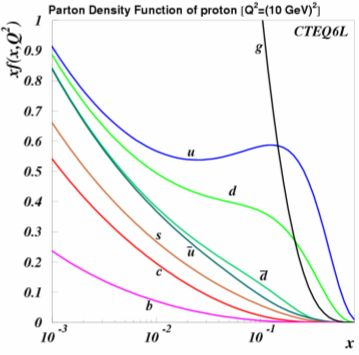
\includegraphics[width=.55\textwidth]{pdf}\hfill\parbox[b]{.44\textwidth}{
\caption{Parton distribution function obtained from the \textsc{cteq} collaboration. It gives the probability of extracting a specific quark from a proton with a certain fraction, $x$ of its energy. From \cite{scien2}.\label{pdff}}}
\end{figure}

While protons contain no antiquarks as valence quarks, every proton is surrounded by a `sea' of virtual particles. At a given energy scale $Q^2$, there is a certain probability for extracting one of these sea quarks in an interaction, given by the Parton Distribution Functions (PDFs), a selection of which is shown in fig.~\ref{pdff}. These functions are found experimentally by several collaborations. This thesis will deal mainly with the CTEQ set of PDFs.

Including this step in the calculation leads to the following expression, which gives the cross section for a diphoton event resulting from a proton-proton collision, $\sigma(pp\rightarrow\gamma\gamma)$ in terms of the $\sigma(q\bar q \rightarrow \gamma\gamma)$ cross section that we have determined thus far:
\[\sigma(pp\rightarrow\gamma\gamma)=\sum_q\iint dx_1\,dx_2\,f_q(x_1,Q^2)f_{\bar q}(x_2,Q^2)\sigma(q\bar q\rightarrow\gamma\gamma),\label{pdf}\]
where $f_q$ is the PDF for parton $q$.


\chapter{Simulation studies}\label{ch.mc}

Now that the theoretical description of the processes under study is in place, we might imagine that obtaining a prediction of the distributions of events that we expect to see in a given experiment is a simple matter of carrying out the integrals found in the previous chapter. Unfortunately, the integrals in question defy analytical solution, which leaves us with the option of integrating numerically. Specifically, we will use the Monte Carlo method for numerical integration, which prescribes inserting a random value drawn from a suitable distribution into the integrand in place of the variable of integration, and then calculating the value of the integrand. Each result estimates the value of the integral, and by averaging a large number of estimates, an incrementally better estimate is obtained.

Since all of the variables that are integrated over have physical significance, choosing specific values for the variables of integration can be viewed as equivalent to laying out the kinematics of a single hypothetical event. Repeatedly estimating the value of the integral a sufficient number of times to obtain a result of passable accuracy from the Monte Carlo integration process in effect leaves us with a large set of simulated events. In particle physics, this process goes by Monte Carlo simulation, and the software packages that are designed to carry out these calculations are called event generators.

\section{Event generators}

The event generator used for the bulk of the work in this thesis is CalcHEP \cite{calchep}. Other choices of event generators include MadGraph \cite{madgraph5} and pythia \cite{pythia}. To illustrate the behaviour of these different generators with respect to one another, figure~\ref{evgen} plots distributions of invariant mass ($M_{\gamma\gamma}$) and transverse momentum ($p_T$) of a set of simulated events generated by each one.

\begin{figure}[hbtp]
\begin{minipage}[b]{.69\textwidth}
\begin{infilsf} \tiny
\hspace{-1ex}\makebox[0pt][l]{\pgfdeclareplotmark{cross} {
\pgfpathmoveto{\pgfpoint{-0.3\pgfplotmarksize}{\pgfplotmarksize}}
\pgfpathlineto{\pgfpoint{+0.3\pgfplotmarksize}{\pgfplotmarksize}}
\pgfpathlineto{\pgfpoint{+0.3\pgfplotmarksize}{0.3\pgfplotmarksize}}
\pgfpathlineto{\pgfpoint{+1\pgfplotmarksize}{0.3\pgfplotmarksize}}
\pgfpathlineto{\pgfpoint{+1\pgfplotmarksize}{-0.3\pgfplotmarksize}}
\pgfpathlineto{\pgfpoint{+0.3\pgfplotmarksize}{-0.3\pgfplotmarksize}}
\pgfpathlineto{\pgfpoint{+0.3\pgfplotmarksize}{-1.\pgfplotmarksize}}
\pgfpathlineto{\pgfpoint{-0.3\pgfplotmarksize}{-1.\pgfplotmarksize}}
\pgfpathlineto{\pgfpoint{-0.3\pgfplotmarksize}{-0.3\pgfplotmarksize}}
\pgfpathlineto{\pgfpoint{-1.\pgfplotmarksize}{-0.3\pgfplotmarksize}}
\pgfpathlineto{\pgfpoint{-1.\pgfplotmarksize}{0.3\pgfplotmarksize}}
\pgfpathlineto{\pgfpoint{-0.3\pgfplotmarksize}{0.3\pgfplotmarksize}}
\pgfpathclose
\pgfusepathqstroke
}
\pgfdeclareplotmark{cross*} {
\pgfpathmoveto{\pgfpoint{-0.3\pgfplotmarksize}{\pgfplotmarksize}}
\pgfpathlineto{\pgfpoint{+0.3\pgfplotmarksize}{\pgfplotmarksize}}
\pgfpathlineto{\pgfpoint{+0.3\pgfplotmarksize}{0.3\pgfplotmarksize}}
\pgfpathlineto{\pgfpoint{+1\pgfplotmarksize}{0.3\pgfplotmarksize}}
\pgfpathlineto{\pgfpoint{+1\pgfplotmarksize}{-0.3\pgfplotmarksize}}
\pgfpathlineto{\pgfpoint{+0.3\pgfplotmarksize}{-0.3\pgfplotmarksize}}
\pgfpathlineto{\pgfpoint{+0.3\pgfplotmarksize}{-1.\pgfplotmarksize}}
\pgfpathlineto{\pgfpoint{-0.3\pgfplotmarksize}{-1.\pgfplotmarksize}}
\pgfpathlineto{\pgfpoint{-0.3\pgfplotmarksize}{-0.3\pgfplotmarksize}}
\pgfpathlineto{\pgfpoint{-1.\pgfplotmarksize}{-0.3\pgfplotmarksize}}
\pgfpathlineto{\pgfpoint{-1.\pgfplotmarksize}{0.3\pgfplotmarksize}}
\pgfpathlineto{\pgfpoint{-0.3\pgfplotmarksize}{0.3\pgfplotmarksize}}
\pgfpathclose
\pgfusepathqfillstroke
}
\pgfdeclareplotmark{newstar} {
\pgfpathmoveto{\pgfqpoint{0pt}{\pgfplotmarksize}}
\pgfpathlineto{\pgfqpointpolar{44}{0.5\pgfplotmarksize}}
\pgfpathlineto{\pgfqpointpolar{18}{\pgfplotmarksize}}
\pgfpathlineto{\pgfqpointpolar{-20}{0.5\pgfplotmarksize}}
\pgfpathlineto{\pgfqpointpolar{-54}{\pgfplotmarksize}}
\pgfpathlineto{\pgfqpointpolar{-90}{0.5\pgfplotmarksize}}
\pgfpathlineto{\pgfqpointpolar{234}{\pgfplotmarksize}}
\pgfpathlineto{\pgfqpointpolar{198}{0.5\pgfplotmarksize}}
\pgfpathlineto{\pgfqpointpolar{162}{\pgfplotmarksize}}
\pgfpathlineto{\pgfqpointpolar{134}{0.5\pgfplotmarksize}}
\pgfpathclose
\pgfusepathqstroke
}
\pgfdeclareplotmark{newstar*} {
\pgfpathmoveto{\pgfqpoint{0pt}{\pgfplotmarksize}}
\pgfpathlineto{\pgfqpointpolar{44}{0.5\pgfplotmarksize}}
\pgfpathlineto{\pgfqpointpolar{18}{\pgfplotmarksize}}
\pgfpathlineto{\pgfqpointpolar{-20}{0.5\pgfplotmarksize}}
\pgfpathlineto{\pgfqpointpolar{-54}{\pgfplotmarksize}}
\pgfpathlineto{\pgfqpointpolar{-90}{0.5\pgfplotmarksize}}
\pgfpathlineto{\pgfqpointpolar{234}{\pgfplotmarksize}}
\pgfpathlineto{\pgfqpointpolar{198}{0.5\pgfplotmarksize}}
\pgfpathlineto{\pgfqpointpolar{162}{\pgfplotmarksize}}
\pgfpathlineto{\pgfqpointpolar{134}{0.5\pgfplotmarksize}}
\pgfpathclose
\pgfusepathqfillstroke
}
\begin{tikzpicture}[x=.045\textwidth,y=.045\textwidth]
\definecolor{c}{rgb}{1,1,1};
\draw [color=c, fill=c] (0,0) rectangle (20,13.5632);
\draw [color=c, fill=c] (0,4.06897) rectangle (20,13.5632);
\draw [color=c, fill=c] (2,4.06897) rectangle (20,13.5632);
\definecolor{c}{rgb}{0,0,0};
\draw [c] (2,4.06897) -- (2,13.5632) -- (20,13.5632) -- (20,4.06897) -- (2,4.06897);
\definecolor{c}{rgb}{1,1,1};
\draw [color=c, fill=c] (2,4.06897) rectangle (20,13.5632);
\definecolor{c}{rgb}{0,0,0};
\draw [c] (2,4.06897) -- (2,13.5632) -- (20,13.5632) -- (20,4.06897) -- (2,4.06897);
\colorlet{c}{kugray};
\draw [c] (2.18,13.2837) -- (2.18,13.2879);
\draw [c] (2.18,13.2879) -- (2.18,13.2921);
\draw [c] (2,13.2879) -- (2.18,13.2879);
\draw [c] (2.18,13.2879) -- (2.36,13.2879);
\draw [c] (2.54,11.6533) -- (2.54,11.6579);
\draw [c] (2.54,11.6579) -- (2.54,11.6625);
\draw [c] (2.36,11.6579) -- (2.54,11.6579);
\draw [c] (2.54,11.6579) -- (2.72,11.6579);
\draw [c] (2.9,10.6843) -- (2.9,10.6987);
\draw [c] (2.9,10.6987) -- (2.9,10.7127);
\draw [c] (2.72,10.6987) -- (2.9,10.6987);
\draw [c] (2.9,10.6987) -- (3.08,10.6987);
\draw [c] (3.26,10.0129) -- (3.26,10.0444);
\draw [c] (3.26,10.0444) -- (3.26,10.0737);
\draw [c] (3.08,10.0444) -- (3.26,10.0444);
\draw [c] (3.26,10.0444) -- (3.44,10.0444);
\draw [c] (3.62,9.42595) -- (3.62,9.48578);
\draw [c] (3.62,9.48578) -- (3.62,9.5382);
\draw [c] (3.44,9.48578) -- (3.62,9.48578);
\draw [c] (3.62,9.48578) -- (3.8,9.48578);
\draw [c] (3.98,8.98638) -- (3.98,9.07402);
\draw [c] (3.98,9.07402) -- (3.98,9.14661);
\draw [c] (3.8,9.07402) -- (3.98,9.07402);
\draw [c] (3.98,9.07402) -- (4.16,9.07402);
\draw [c] (4.34,8.63304) -- (4.34,8.69108);
\draw [c] (4.34,8.69108) -- (4.34,8.74213);
\draw [c] (4.16,8.69108) -- (4.34,8.69108);
\draw [c] (4.34,8.69108) -- (4.52,8.69108);
\draw [c] (4.7,8.29897) -- (4.7,8.30433);
\draw [c] (4.7,8.30433) -- (4.7,8.30962);
\draw [c] (4.52,8.30433) -- (4.7,8.30433);
\draw [c] (4.7,8.30433) -- (4.88,8.30433);
\draw [c] (5.06,7.93898) -- (5.06,7.94717);
\draw [c] (5.06,7.94717) -- (5.06,7.9552);
\draw [c] (4.88,7.94717) -- (5.06,7.94717);
\draw [c] (5.06,7.94717) -- (5.24,7.94717);
\draw [c] (5.42,7.61222) -- (5.42,7.62426);
\draw [c] (5.42,7.62426) -- (5.42,7.63596);
\draw [c] (5.24,7.62426) -- (5.42,7.62426);
\draw [c] (5.42,7.62426) -- (5.6,7.62426);
\draw [c] (5.78,7.30901) -- (5.78,7.32622);
\draw [c] (5.78,7.32622) -- (5.78,7.34275);
\draw [c] (5.6,7.32622) -- (5.78,7.32622);
\draw [c] (5.78,7.32622) -- (5.96,7.32622);
\draw [c] (6.14,6.96941) -- (6.14,6.99508);
\draw [c] (6.14,6.99508) -- (6.14,7.01929);
\draw [c] (5.96,6.99508) -- (6.14,6.99508);
\draw [c] (6.14,6.99508) -- (6.32,6.99508);
\draw [c] (6.5,6.65186) -- (6.5,6.68918);
\draw [c] (6.5,6.68918) -- (6.5,6.72348);
\draw [c] (6.32,6.68918) -- (6.5,6.68918);
\draw [c] (6.5,6.68918) -- (6.68,6.68918);
\draw [c] (6.86,6.31826) -- (6.86,6.37354);
\draw [c] (6.86,6.37354) -- (6.86,6.42243);
\draw [c] (6.68,6.37354) -- (6.86,6.37354);
\draw [c] (6.86,6.37354) -- (7.04,6.37354);
\draw [c] (7.22,6.04546) -- (7.22,6.12165);
\draw [c] (7.22,6.12165) -- (7.22,6.18622);
\draw [c] (7.04,6.12165) -- (7.22,6.12165);
\draw [c] (7.22,6.12165) -- (7.4,6.12165);
\draw [c] (7.58,5.86069) -- (7.58,5.95535);
\draw [c] (7.58,5.95535) -- (7.58,6.03269);
\draw [c] (7.4,5.95535) -- (7.58,5.95535);
\draw [c] (7.58,5.95535) -- (7.76,5.95535);
\draw [c] (7.94,5.57747) -- (7.94,5.70938);
\draw [c] (7.94,5.70938) -- (7.94,5.80986);
\draw [c] (7.76,5.70938) -- (7.94,5.70938);
\draw [c] (7.94,5.70938) -- (8.12,5.70938);
\draw [c] (8.3,4.88391) -- (8.3,5.17795);
\draw [c] (8.3,5.17795) -- (8.3,5.34995);
\draw [c] (8.12,5.17795) -- (8.3,5.17795);
\draw [c] (8.3,5.17795) -- (8.48,5.17795);
\draw [c] (8.66,4.363) -- (8.66,4.88391);
\draw [c] (8.66,4.88391) -- (8.66,5.11078);
\draw [c] (8.48,4.88391) -- (8.66,4.88391);
\draw [c] (8.66,4.88391) -- (8.84,4.88391);
\draw [c] (9.02,4.06897) -- (9.02,4.58987);
\draw [c] (9.02,4.58987) -- (9.02,4.88391);
\draw [c] (8.84,4.58987) -- (9.02,4.58987);
\draw [c] (9.02,4.58987) -- (9.2,4.58987);
\draw [c] (9.38,4.06897) -- (9.38,4.58987);
\draw [c] (9.38,4.58987) -- (9.38,4.88391);
\draw [c] (9.2,4.58987) -- (9.38,4.58987);
\draw [c] (9.38,4.58987) -- (9.56,4.58987);
\draw [c] (9.74,4.06897) -- (9.74,4.58987);
\draw [c] (9.74,4.58987) -- (9.74,4.88391);
\draw [c] (9.56,4.58987) -- (9.74,4.58987);
\draw [c] (9.74,4.58987) -- (9.92,4.58987);
\draw [c] (10.1,4.06897) -- (10.1,4.58987);
\draw [c] (10.1,4.58987) -- (10.1,4.88391);
\draw [c] (9.92,4.58987) -- (10.1,4.58987);
\draw [c] (10.1,4.58987) -- (10.28,4.58987);
\draw [c] (10.82,4.363) -- (10.82,4.88391);
\draw [c] (10.82,4.88391) -- (10.82,5.11078);
\draw [c] (10.64,4.88391) -- (10.82,4.88391);
\draw [c] (10.82,4.88391) -- (11,4.88391);
\definecolor{c}{rgb}{0,0,0};
\draw [c] (2,4.06897) -- (20,4.06897);
\draw [c] (2,4.32531) -- (2,4.06897);
\draw [c] (2.45,4.19714) -- (2.45,4.06897);
\draw [c] (2.9,4.19714) -- (2.9,4.06897);
\draw [c] (3.35,4.19714) -- (3.35,4.06897);
\draw [c] (3.8,4.19714) -- (3.8,4.06897);
\draw [c] (4.25,4.32531) -- (4.25,4.06897);
\draw [c] (4.7,4.19714) -- (4.7,4.06897);
\draw [c] (5.15,4.19714) -- (5.15,4.06897);
\draw [c] (5.6,4.19714) -- (5.6,4.06897);
\draw [c] (6.05,4.19714) -- (6.05,4.06897);
\draw [c] (6.5,4.32531) -- (6.5,4.06897);
\draw [c] (6.95,4.19714) -- (6.95,4.06897);
\draw [c] (7.4,4.19714) -- (7.4,4.06897);
\draw [c] (7.85,4.19714) -- (7.85,4.06897);
\draw [c] (8.3,4.19714) -- (8.3,4.06897);
\draw [c] (8.75,4.32531) -- (8.75,4.06897);
\draw [c] (9.2,4.19714) -- (9.2,4.06897);
\draw [c] (9.65,4.19714) -- (9.65,4.06897);
\draw [c] (10.1,4.19714) -- (10.1,4.06897);
\draw [c] (10.55,4.19714) -- (10.55,4.06897);
\draw [c] (11,4.32531) -- (11,4.06897);
\draw [c] (11.45,4.19714) -- (11.45,4.06897);
\draw [c] (11.9,4.19714) -- (11.9,4.06897);
\draw [c] (12.35,4.19714) -- (12.35,4.06897);
\draw [c] (12.8,4.19714) -- (12.8,4.06897);
\draw [c] (13.25,4.32531) -- (13.25,4.06897);
\draw [c] (13.7,4.19714) -- (13.7,4.06897);
\draw [c] (14.15,4.19714) -- (14.15,4.06897);
\draw [c] (14.6,4.19714) -- (14.6,4.06897);
\draw [c] (15.05,4.19714) -- (15.05,4.06897);
\draw [c] (15.5,4.32531) -- (15.5,4.06897);
\draw [c] (15.95,4.19714) -- (15.95,4.06897);
\draw [c] (16.4,4.19714) -- (16.4,4.06897);
\draw [c] (16.85,4.19714) -- (16.85,4.06897);
\draw [c] (17.3,4.19714) -- (17.3,4.06897);
\draw [c] (17.75,4.32531) -- (17.75,4.06897);
\draw [c] (18.2,4.19714) -- (18.2,4.06897);
\draw [c] (18.65,4.19714) -- (18.65,4.06897);
\draw [c] (19.1,4.19714) -- (19.1,4.06897);
\draw [c] (19.55,4.19714) -- (19.55,4.06897);
\draw [c] (20,4.32531) -- (20,4.06897);
\draw [c] (2,4.32531) -- (2,4.06897);
\draw [c] (20,4.32531) -- (20,4.06897);

\draw [c] (2,4.06897) -- (2,13.5632);
\draw [anchor= east] (0.1,13.5632) node[ rotate=90]{$\di\sigma/\di p_T^{\gamma_1} \text{ [pb/GeV]}$};
\draw [c] (2.3,4.11929) -- (2,4.11929);
\draw [c] (2.3,4.16926) -- (2,4.16926);
\draw [c] (2.6,4.21395) -- (2,4.21395);
\draw [anchor= east] (1.844,4.21395) node[ rotate=0]{$10^{-10}$};
\draw [c] (2.3,4.50799) -- (2,4.50799);
\draw [c] (2.3,4.67999) -- (2,4.67999);
\draw [c] (2.3,4.80203) -- (2,4.80203);
\draw [c] (2.3,4.89669) -- (2,4.89669);
\draw [c] (2.3,4.97403) -- (2,4.97403);
\draw [c] (2.3,5.03942) -- (2,5.03942);
\draw [c] (2.3,5.09607) -- (2,5.09607);
\draw [c] (2.3,5.14603) -- (2,5.14603);
\draw [c] (2.6,5.19073) -- (2,5.19073);
\draw [anchor= east] (1.844,5.19073) node[ rotate=0]{$10^{-9}$};
\draw [c] (2.3,5.48477) -- (2,5.48477);
\draw [c] (2.3,5.65677) -- (2,5.65677);
\draw [c] (2.3,5.77881) -- (2,5.77881);
\draw [c] (2.3,5.87347) -- (2,5.87347);
\draw [c] (2.3,5.95081) -- (2,5.95081);
\draw [c] (2.3,6.0162) -- (2,6.0162);
\draw [c] (2.3,6.07284) -- (2,6.07284);
\draw [c] (2.3,6.12281) -- (2,6.12281);
\draw [c] (2.6,6.1675) -- (2,6.1675);
\draw [anchor= east] (1.844,6.1675) node[ rotate=0]{$10^{-8}$};
\draw [c] (2.3,6.46154) -- (2,6.46154);
\draw [c] (2.3,6.63354) -- (2,6.63354);
\draw [c] (2.3,6.75558) -- (2,6.75558);
\draw [c] (2.3,6.85024) -- (2,6.85024);
\draw [c] (2.3,6.92758) -- (2,6.92758);
\draw [c] (2.3,6.99298) -- (2,6.99298);
\draw [c] (2.3,7.04962) -- (2,7.04962);
\draw [c] (2.3,7.09959) -- (2,7.09959);
\draw [c] (2.6,7.14428) -- (2,7.14428);
\draw [anchor= east] (1.844,7.14428) node[ rotate=0]{$10^{-7}$};
\draw [c] (2.3,7.43832) -- (2,7.43832);
\draw [c] (2.3,7.61032) -- (2,7.61032);
\draw [c] (2.3,7.73236) -- (2,7.73236);
\draw [c] (2.3,7.82702) -- (2,7.82702);
\draw [c] (2.3,7.90436) -- (2,7.90436);
\draw [c] (2.3,7.96975) -- (2,7.96975);
\draw [c] (2.3,8.0264) -- (2,8.0264);
\draw [c] (2.3,8.07636) -- (2,8.07636);
\draw [c] (2.6,8.12106) -- (2,8.12106);
\draw [anchor= east] (1.844,8.12106) node[ rotate=0]{$10^{-6}$};
\draw [c] (2.3,8.4151) -- (2,8.4151);
\draw [c] (2.3,8.5871) -- (2,8.5871);
\draw [c] (2.3,8.70914) -- (2,8.70914);
\draw [c] (2.3,8.80379) -- (2,8.80379);
\draw [c] (2.3,8.88114) -- (2,8.88114);
\draw [c] (2.3,8.94653) -- (2,8.94653);
\draw [c] (2.3,9.00317) -- (2,9.00317);
\draw [c] (2.3,9.05314) -- (2,9.05314);
\draw [c] (2.6,9.09783) -- (2,9.09783);
\draw [anchor= east] (1.844,9.09783) node[ rotate=0]{$10^{-5}$};
\draw [c] (2.3,9.39187) -- (2,9.39187);
\draw [c] (2.3,9.56387) -- (2,9.56387);
\draw [c] (2.3,9.68591) -- (2,9.68591);
\draw [c] (2.3,9.78057) -- (2,9.78057);
\draw [c] (2.3,9.85791) -- (2,9.85791);
\draw [c] (2.3,9.9233) -- (2,9.9233);
\draw [c] (2.3,9.97995) -- (2,9.97995);
\draw [c] (2.3,10.0299) -- (2,10.0299);
\draw [c] (2.6,10.0746) -- (2,10.0746);
\draw [anchor= east] (1.844,10.0746) node[ rotate=0]{$10^{-4}$};
\draw [c] (2.3,10.3686) -- (2,10.3686);
\draw [c] (2.3,10.5407) -- (2,10.5407);
\draw [c] (2.3,10.6627) -- (2,10.6627);
\draw [c] (2.3,10.7573) -- (2,10.7573);
\draw [c] (2.3,10.8347) -- (2,10.8347);
\draw [c] (2.3,10.9001) -- (2,10.9001);
\draw [c] (2.3,10.9567) -- (2,10.9567);
\draw [c] (2.3,11.0067) -- (2,11.0067);
\draw [c] (2.6,11.0514) -- (2,11.0514);
\draw [anchor= east] (1.844,11.0514) node[ rotate=0]{$10^{-3}$};
\draw [c] (2.3,11.3454) -- (2,11.3454);
\draw [c] (2.3,11.5174) -- (2,11.5174);
\draw [c] (2.3,11.6395) -- (2,11.6395);
\draw [c] (2.3,11.7341) -- (2,11.7341);
\draw [c] (2.3,11.8115) -- (2,11.8115);
\draw [c] (2.3,11.8769) -- (2,11.8769);
\draw [c] (2.3,11.9335) -- (2,11.9335);
\draw [c] (2.3,11.9835) -- (2,11.9835);
\draw [c] (2.6,12.0282) -- (2,12.0282);
\draw [anchor= east] (1.844,12.0282) node[ rotate=0]{$10^{-2}$};
\draw [c] (2.3,12.3222) -- (2,12.3222);
\draw [c] (2.3,12.4942) -- (2,12.4942);
\draw [c] (2.3,12.6162) -- (2,12.6162);
\draw [c] (2.3,12.7109) -- (2,12.7109);
\draw [c] (2.3,12.7882) -- (2,12.7882);
\draw [c] (2.3,12.8536) -- (2,12.8536);
\draw [c] (2.3,12.9103) -- (2,12.9103);
\draw [c] (2.3,12.9602) -- (2,12.9602);
\draw [c] (2.6,13.0049) -- (2,13.0049);
\draw [anchor= east] (1.844,13.0049) node[ rotate=0]{$10^{-1}$};
\draw [c] (2.3,13.299) -- (2,13.299);
\draw [c] (2.3,13.471) -- (2,13.471);
\colorlet{c}{natgreen};
\draw [c] (2.18,13.2731) -- (2.18,13.2747);
\draw [c] (2.18,13.2747) -- (2.18,13.2763);
\draw [c] (2,13.2747) -- (2.18,13.2747);
\draw [c] (2.18,13.2747) -- (2.36,13.2747);
\draw [c] (2.54,11.6659) -- (2.54,11.6765);
\draw [c] (2.54,11.6765) -- (2.54,11.6869);
\draw [c] (2.36,11.6765) -- (2.54,11.6765);
\draw [c] (2.54,11.6765) -- (2.72,11.6765);
\draw [c] (2.9,10.6691) -- (2.9,10.6978);
\draw [c] (2.9,10.6978) -- (2.9,10.7246);
\draw [c] (2.72,10.6978) -- (2.9,10.6978);
\draw [c] (2.9,10.6978) -- (3.08,10.6978);
\draw [c] (3.26,10.0576) -- (3.26,10.0601);
\draw [c] (3.26,10.0601) -- (3.26,10.0626);
\draw [c] (3.08,10.0601) -- (3.26,10.0601);
\draw [c] (3.26,10.0601) -- (3.44,10.0601);
\draw [c] (3.62,9.53583) -- (3.62,9.54042);
\draw [c] (3.62,9.54042) -- (3.62,9.54496);
\draw [c] (3.44,9.54042) -- (3.62,9.54042);
\draw [c] (3.62,9.54042) -- (3.8,9.54042);
\draw [c] (3.98,9.09436) -- (3.98,9.10208);
\draw [c] (3.98,9.10208) -- (3.98,9.10966);
\draw [c] (3.8,9.10208) -- (3.98,9.10208);
\draw [c] (3.98,9.10208) -- (4.16,9.10208);
\draw [c] (4.34,8.69455) -- (4.34,8.70691);
\draw [c] (4.34,8.70691) -- (4.34,8.71893);
\draw [c] (4.16,8.70691) -- (4.34,8.70691);
\draw [c] (4.34,8.70691) -- (4.52,8.70691);
\draw [c] (4.7,8.29362) -- (4.7,8.31346);
\draw [c] (4.7,8.31346) -- (4.7,8.33241);
\draw [c] (4.52,8.31346) -- (4.7,8.31346);
\draw [c] (4.7,8.31346) -- (4.88,8.31346);
\draw [c] (5.06,7.93123) -- (5.06,7.96164);
\draw [c] (5.06,7.96164) -- (5.06,7.99001);
\draw [c] (4.88,7.96164) -- (5.06,7.96164);
\draw [c] (5.06,7.96164) -- (5.24,7.96164);
\draw [c] (5.42,7.62606) -- (5.42,7.66962);
\draw [c] (5.42,7.66962) -- (5.42,7.70912);
\draw [c] (5.24,7.66962) -- (5.42,7.66962);
\draw [c] (5.42,7.66962) -- (5.6,7.66962);
\draw [c] (5.78,7.35019) -- (5.78,7.41047);
\draw [c] (5.78,7.41047) -- (5.78,7.46323);
\draw [c] (5.6,7.41047) -- (5.78,7.41047);
\draw [c] (5.78,7.41047) -- (5.96,7.41047);
\draw [c] (6.14,7.05267) -- (6.14,7.13819);
\draw [c] (6.14,7.13819) -- (6.14,7.20933);
\draw [c] (5.96,7.13819) -- (6.14,7.13819);
\draw [c] (6.14,7.13819) -- (6.32,7.13819);
\draw [c] (6.5,6.65721) -- (6.5,6.75996);
\draw [c] (6.5,6.75996) -- (6.5,6.84262);
\draw [c] (6.32,6.75996) -- (6.5,6.75996);
\draw [c] (6.5,6.75996) -- (6.68,6.75996);
\draw [c] (6.86,6.49404) -- (6.86,6.49634);
\draw [c] (6.86,6.49634) -- (6.86,6.49863);
\draw [c] (6.68,6.49634) -- (6.86,6.49634);
\draw [c] (6.86,6.49634) -- (7.04,6.49634);
\draw [c] (7.22,6.2213) -- (7.22,6.22448);
\draw [c] (7.22,6.22448) -- (7.22,6.22762);
\draw [c] (7.04,6.22448) -- (7.22,6.22448);
\draw [c] (7.22,6.22448) -- (7.4,6.22448);
\draw [c] (7.58,5.94687) -- (7.58,5.95125);
\draw [c] (7.58,5.95125) -- (7.58,5.95559);
\draw [c] (7.4,5.95125) -- (7.58,5.95125);
\draw [c] (7.58,5.95125) -- (7.76,5.95125);
\draw [c] (7.94,5.68108) -- (7.94,5.68708);
\draw [c] (7.94,5.68708) -- (7.94,5.69299);
\draw [c] (7.76,5.68708) -- (7.94,5.68708);
\draw [c] (7.94,5.68708) -- (8.12,5.68708);
\draw [c] (8.3,5.4057) -- (8.3,5.414);
\draw [c] (8.3,5.414) -- (8.3,5.42213);
\draw [c] (8.12,5.414) -- (8.3,5.414);
\draw [c] (8.3,5.414) -- (8.48,5.414);
\draw [c] (8.66,5.14525) -- (8.66,5.15652);
\draw [c] (8.66,5.15652) -- (8.66,5.16751);
\draw [c] (8.48,5.15652) -- (8.66,5.15652);
\draw [c] (8.66,5.15652) -- (8.84,5.15652);
\draw [c] (9.02,4.91326) -- (9.02,4.92808);
\draw [c] (9.02,4.92808) -- (9.02,4.94241);
\draw [c] (8.84,4.92808) -- (9.02,4.92808);
\draw [c] (9.02,4.92808) -- (9.2,4.92808);
\draw [c] (9.38,4.59832) -- (9.38,4.6198);
\draw [c] (9.38,4.6198) -- (9.38,4.64025);
\draw [c] (9.2,4.6198) -- (9.38,4.6198);
\draw [c] (9.38,4.6198) -- (9.56,4.6198);
\draw [c] (9.74,4.32611) -- (9.74,4.35572);
\draw [c] (9.74,4.35572) -- (9.74,4.3834);
\draw [c] (9.56,4.35572) -- (9.74,4.35572);
\draw [c] (9.74,4.35572) -- (9.92,4.35572);
\draw [c] (10.1,4.06897) -- (10.1,4.08054);
\draw [c] (10.1,4.08054) -- (10.1,4.11836);
\draw [c] (9.92,4.08054) -- (10.1,4.08054);
\draw [c] (10.1,4.08054) -- (10.28,4.08054);
\colorlet{c}{natcomp};
\draw [c] (2.18,13.3011) -- (2.18,13.302);
\draw [c] (2.18,13.302) -- (2.18,13.3029);
\draw [c] (2,13.302) -- (2.18,13.302);
\draw [c] (2.18,13.302) -- (2.36,13.302);
\draw [c] (2.54,11.6649) -- (2.54,11.6713);
\draw [c] (2.54,11.6713) -- (2.54,11.6775);
\draw [c] (2.36,11.6713) -- (2.54,11.6713);
\draw [c] (2.54,11.6713) -- (2.72,11.6713);
\draw [c] (2.9,10.6525) -- (2.9,10.6734);
\draw [c] (2.9,10.6734) -- (2.9,10.6934);
\draw [c] (2.72,10.6734) -- (2.9,10.6734);
\draw [c] (2.9,10.6734) -- (3.08,10.6734);
\draw [c] (3.26,9.90775) -- (3.26,9.95804);
\draw [c] (3.26,9.95804) -- (3.26,10.003);
\draw [c] (3.08,9.95804) -- (3.26,9.95804);
\draw [c] (3.26,9.95804) -- (3.44,9.95804);
\draw [c] (3.62,9.51424) -- (3.62,9.5169);
\draw [c] (3.62,9.5169) -- (3.62,9.51955);
\draw [c] (3.44,9.5169) -- (3.62,9.5169);
\draw [c] (3.62,9.5169) -- (3.8,9.5169);
\draw [c] (3.98,9.06341) -- (3.98,9.06795);
\draw [c] (3.98,9.06795) -- (3.98,9.07243);
\draw [c] (3.8,9.06795) -- (3.98,9.06795);
\draw [c] (3.98,9.06795) -- (4.16,9.06795);
\draw [c] (4.34,8.64794) -- (4.34,8.65534);
\draw [c] (4.34,8.65534) -- (4.34,8.6626);
\draw [c] (4.16,8.65534) -- (4.34,8.65534);
\draw [c] (4.34,8.65534) -- (4.52,8.65534);
\draw [c] (4.7,8.23698) -- (4.7,8.24899);
\draw [c] (4.7,8.24899) -- (4.7,8.26066);
\draw [c] (4.52,8.24899) -- (4.7,8.24899);
\draw [c] (4.7,8.24899) -- (4.88,8.24899);
\draw [c] (5.06,7.90895) -- (5.06,7.92662);
\draw [c] (5.06,7.92662) -- (5.06,7.94358);
\draw [c] (4.88,7.92662) -- (5.06,7.92662);
\draw [c] (5.06,7.92662) -- (5.24,7.92662);
\draw [c] (5.42,7.57803) -- (5.42,7.60412);
\draw [c] (5.42,7.60412) -- (5.42,7.6287);
\draw [c] (5.24,7.60412) -- (5.42,7.60412);
\draw [c] (5.42,7.60412) -- (5.6,7.60412);
\draw [c] (5.78,7.23476) -- (5.78,7.27386);
\draw [c] (5.78,7.27386) -- (5.78,7.30965);
\draw [c] (5.6,7.27386) -- (5.78,7.27386);
\draw [c] (5.78,7.27386) -- (5.96,7.27386);
\draw [c] (6.14,6.91271) -- (6.14,6.96983);
\draw [c] (6.14,6.96983) -- (6.14,7.02017);
\draw [c] (5.96,6.96983) -- (6.14,6.96983);
\draw [c] (6.14,6.96983) -- (6.32,6.96983);
\draw [c] (6.5,6.55358) -- (6.5,6.64072);
\draw [c] (6.5,6.64072) -- (6.5,6.71297);
\draw [c] (6.32,6.64072) -- (6.5,6.64072);
\draw [c] (6.5,6.64072) -- (6.68,6.64072);
\draw [c] (6.86,6.0278) -- (6.86,6.18906);
\draw [c] (6.86,6.18906) -- (6.86,6.30562);
\draw [c] (6.68,6.18906) -- (6.86,6.18906);
\draw [c] (6.86,6.18906) -- (7.04,6.18906);
\draw [c] (7.22,6.1219) -- (7.22,6.2664);
\draw [c] (7.22,6.2664) -- (7.22,6.37399);
\draw [c] (7.04,6.2664) -- (7.22,6.2664);
\draw [c] (7.22,6.2664) -- (7.4,6.2664);
\draw [c] (7.58,4.98541) -- (7.58,5.50632);
\draw [c] (7.58,5.50632) -- (7.58,5.73319);
\draw [c] (7.4,5.50632) -- (7.58,5.50632);
\draw [c] (7.58,5.50632) -- (7.76,5.50632);
\draw [c] (7.94,4.98541) -- (7.94,5.50632);
\draw [c] (7.94,5.50632) -- (7.94,5.73319);
\draw [c] (7.76,5.50632) -- (7.94,5.50632);
\draw [c] (7.94,5.50632) -- (8.12,5.50632);
\draw [c] (8.66,4.06897) -- (8.66,5.21228);
\draw [c] (8.66,5.21228) -- (8.66,5.50632);
\draw [c] (8.48,5.21228) -- (8.66,5.21228);
\draw [c] (8.66,5.21228) -- (8.84,5.21228);
\draw [c] (9.74,4.06897) -- (9.74,5.21228);
\draw [c] (9.74,5.21228) -- (9.74,5.50632);
\draw [c] (9.56,5.21228) -- (9.74,5.21228);
\draw [c] (9.74,5.21228) -- (9.92,5.21228);
\definecolor{c}{rgb}{1,1,1};
\draw [c] (14.1954,11.0057) -- (14.1954,12.9598) -- (19.8851,12.9598) -- (19.8851,11.0057) -- (14.1954,11.0057);
\draw [c] (14.1954,11.0057) -- (19.8851,11.0057);
\draw [c] (19.8851,11.0057) -- (19.8851,12.9598);
\draw [c] (19.8851,12.9598) -- (14.1954,12.9598);
\draw [c] (14.1954,12.9598) -- (14.1954,11.0057);
\draw [anchor=base west] (15.6178,12.4875) node[ rotate=0]{CalcHEP};
\colorlet{c}{kugray!20};
\draw [c, fill=c] (14.4088,12.4061) -- (15.4045,12.4061) -- (15.4045,12.8621) -- (14.4088,12.8621);
\colorlet{c}{kugray};
\draw [c] (14.4088,12.6341) -- (15.4045,12.6341);
\draw [anchor=base west] (15.6178,11.8362) node[ rotate=0]{pythia8};
\colorlet{c}{natgreen};
\draw [c] (14.4088,11.9828) -- (15.4045,11.9828);
\draw [anchor=base west] (15.6178,11.1849) node[ rotate=0]{MadGraph};
\colorlet{c}{natcomp};
\draw [c] (14.4088,11.3314) -- (15.4045,11.3314);
% \definecolor{c}{rgb}{1,1,1};
% \draw [color=c, fill=c] (0,0) rectangle (20,4.06897);
% \draw [color=c, fill=c] (2,0.406897) rectangle (20,4.06897);
% \definecolor{c}{rgb}{0,0,0};
% \draw [c] (2,0.406897) -- (2,4.06897) -- (20,4.06897) -- (20,0.406897) -- (2,0.406897);
% \definecolor{c}{rgb}{1,1,1};
% \draw [color=c, fill=c] (2,0.406897) rectangle (20,4.06897);
\colorlet{c}{kugray!20};
\draw [color=c, fill=c] (2,2.30251) rectangle (2.36,2.36595);
\draw [color=c, fill=c] (2.36,2.29952) rectangle (2.72,2.36893);
\draw [color=c, fill=c] (2.72,2.2269) rectangle (3.08,2.44155);
\draw [color=c, fill=c] (3.08,2.10501) rectangle (3.44,2.56344);
\draw [color=c, fill=c] (3.44,1.9124) rectangle (3.8,2.75606);
\draw [color=c, fill=c] (3.8,1.73569) rectangle (4.16,2.93277);
\draw [color=c, fill=c] (4.16,1.92417) rectangle (4.52,2.74429);
\draw [color=c, fill=c] (4.52,2.29398) rectangle (4.88,2.37447);
\draw [color=c, fill=c] (4.88,2.27292) rectangle (5.24,2.39554);
\draw [color=c, fill=c] (5.24,2.24452) rectangle (5.6,2.42393);
\draw [color=c, fill=c] (5.6,2.20677) rectangle (5.96,2.46169);
\draw [color=c, fill=c] (5.96,2.14591) rectangle (6.32,2.52254);
\draw [color=c, fill=c] (6.32,2.06416) rectangle (6.68,2.60429);
\draw [color=c, fill=c] (6.68,1.94245) rectangle (7.04,2.72601);
\draw [color=c, fill=c] (7.04,1.80702) rectangle (7.4,2.86143);
\draw [color=c, fill=c] (7.4,1.69286) rectangle (7.76,2.9756);
\draw [color=c, fill=c] (7.76,1.47716) rectangle (8.12,3.1913);
\draw [color=c, fill=c] (8.12,0.730798) rectangle (8.48,3.93766);
\draw [color=c, fill=c] (8.48,0.406897) rectangle (8.84,4.06897);
\draw [color=c, fill=c] (8.84,0.406897) rectangle (9.2,4.06897);
\draw [color=c, fill=c] (9.2,0.406897) rectangle (9.56,4.06897);
\draw [color=c, fill=c] (9.56,0.406897) rectangle (9.92,4.06897);
\draw [color=c, fill=c] (9.92,0.406897) rectangle (10.28,4.06897);
\draw [color=c, fill=c] (10.28,2.33423) rectangle (10.64,2.33423);
\draw [color=c, fill=c] (10.64,0.406897) rectangle (11,4.06897);
\draw [color=c, fill=c] (11,2.33423) rectangle (11.36,2.33423);
\draw [color=c, fill=c] (11.36,2.33423) rectangle (11.72,2.33423);
\draw [color=c, fill=c] (11.72,2.33423) rectangle (12.08,2.33423);
\draw [color=c, fill=c] (12.08,2.33423) rectangle (12.44,2.33423);
\draw [color=c, fill=c] (12.44,2.33423) rectangle (12.8,2.33423);
\draw [color=c, fill=c] (12.8,2.33423) rectangle (13.16,2.33423);
\draw [color=c, fill=c] (13.16,2.33423) rectangle (13.52,2.33423);
\draw [color=c, fill=c] (13.52,2.33423) rectangle (13.88,2.33423);
\draw [color=c, fill=c] (13.88,2.33423) rectangle (14.24,2.33423);
\draw [color=c, fill=c] (14.24,2.33423) rectangle (14.6,2.33423);
\draw [color=c, fill=c] (14.6,2.33423) rectangle (14.96,2.33423);
\draw [color=c, fill=c] (14.96,2.33423) rectangle (15.32,2.33423);
\draw [color=c, fill=c] (15.32,2.33423) rectangle (15.68,2.33423);
\draw [color=c, fill=c] (15.68,2.33423) rectangle (16.04,2.33423);
\draw [color=c, fill=c] (16.04,2.33423) rectangle (16.4,2.33423);
\draw [color=c, fill=c] (16.4,2.33423) rectangle (16.76,2.33423);
\draw [color=c, fill=c] (16.76,2.33423) rectangle (17.12,2.33423);
\draw [color=c, fill=c] (17.12,2.33423) rectangle (17.48,2.33423);
\draw [color=c, fill=c] (17.48,2.33423) rectangle (17.84,2.33423);
\draw [color=c, fill=c] (17.84,2.33423) rectangle (18.2,2.33423);
\draw [color=c, fill=c] (18.2,2.33423) rectangle (18.56,2.33423);
\draw [color=c, fill=c] (18.56,2.33423) rectangle (18.92,2.33423);
\draw [color=c, fill=c] (18.92,2.33423) rectangle (19.28,2.33423);
\draw [color=c, fill=c] (19.28,2.33423) rectangle (19.64,2.33423);
\draw [color=c, fill=c] (19.64,2.33423) rectangle (20,2.33423);
\definecolor{c}{rgb}{0,0,0};
\draw [c] (2,0.406897) -- (20,0.406897);
\draw [anchor= east] (20,0.179034) +(0,-2em) node[ rotate=0]{$p_T^{\gamma_1} \text{ [GeV]}$};
\draw [c] (2,0.516759) -- (2,0.406897);
\draw [c] (2.45,0.461828) -- (2.45,0.406897);
\draw [c] (2.9,0.461828) -- (2.9,0.406897);
\draw [c] (3.35,0.461828) -- (3.35,0.406897);
\draw [c] (3.8,0.461828) -- (3.8,0.406897);
\draw [c] (4.25,0.516759) -- (4.25,0.406897);
\draw [c] (4.7,0.461828) -- (4.7,0.406897);
\draw [c] (5.15,0.461828) -- (5.15,0.406897);
\draw [c] (5.6,0.461828) -- (5.6,0.406897);
\draw [c] (6.05,0.461828) -- (6.05,0.406897);
\draw [c] (6.5,0.516759) -- (6.5,0.406897);
\draw [c] (6.95,0.461828) -- (6.95,0.406897);
\draw [c] (7.4,0.461828) -- (7.4,0.406897);
\draw [c] (7.85,0.461828) -- (7.85,0.406897);
\draw [c] (8.3,0.461828) -- (8.3,0.406897);
\draw [c] (8.75,0.516759) -- (8.75,0.406897);
\draw [c] (9.2,0.461828) -- (9.2,0.406897);
\draw [c] (9.65,0.461828) -- (9.65,0.406897);
\draw [c] (10.1,0.461828) -- (10.1,0.406897);
\draw [c] (10.55,0.461828) -- (10.55,0.406897);
\draw [c] (11,0.516759) -- (11,0.406897);
\draw [c] (11.45,0.461828) -- (11.45,0.406897);
\draw [c] (11.9,0.461828) -- (11.9,0.406897);
\draw [c] (12.35,0.461828) -- (12.35,0.406897);
\draw [c] (12.8,0.461828) -- (12.8,0.406897);
\draw [c] (13.25,0.516759) -- (13.25,0.406897);
\draw [c] (13.7,0.461828) -- (13.7,0.406897);
\draw [c] (14.15,0.461828) -- (14.15,0.406897);
\draw [c] (14.6,0.461828) -- (14.6,0.406897);
\draw [c] (15.05,0.461828) -- (15.05,0.406897);
\draw [c] (15.5,0.516759) -- (15.5,0.406897);
\draw [c] (15.95,0.461828) -- (15.95,0.406897);
\draw [c] (16.4,0.461828) -- (16.4,0.406897);
\draw [c] (16.85,0.461828) -- (16.85,0.406897);
\draw [c] (17.3,0.461828) -- (17.3,0.406897);
\draw [c] (17.75,0.516759) -- (17.75,0.406897);
\draw [c] (18.2,0.461828) -- (18.2,0.406897);
\draw [c] (18.65,0.461828) -- (18.65,0.406897);
\draw [c] (19.1,0.461828) -- (19.1,0.406897);
\draw [c] (19.55,0.461828) -- (19.55,0.406897);
\draw [c] (20,0.516759) -- (20,0.406897);
\draw [c] (2,0.516759) -- (2,0.406897);
\draw [c] (20,0.516759) -- (20,0.406897);
\draw [anchor=base] (2,0.272621)     +(0,-.9em) node[ rotate=0]{0};
\draw [anchor=base] (4.25,0.272621)  +(0,-.9em) node[ rotate=0]{500};
\draw [anchor=base] (6.5,0.272621)   +(0,-.9em) node[ rotate=0]{1000};
\draw [anchor=base] (8.75,0.272621)  +(0,-.9em) node[ rotate=0]{1500};
\draw [anchor=base] (11,0.272621)    +(0,-.9em) node[ rotate=0]{2000};
\draw [anchor=base] (13.25,0.272621) +(0,-.9em) node[ rotate=0]{2500};
\draw [anchor=base] (15.5,0.272621)  +(0,-.9em) node[ rotate=0]{3000};
\draw [anchor=base] (17.75,0.272621) +(0,-.9em) node[ rotate=0]{3500};
\draw [anchor=base] (20,0.272621)    +(0,-.9em) node[ rotate=0]{4000};
\draw [c] (2,0.406897) -- (2,4.06897);
\draw [anchor= east] (0.1,4.06897) node[ rotate=90]{Ratio};
\draw [c] (2.54,1.20043) -- (2,1.20043);
\draw [c] (2.27,1.42719) -- (2,1.42719);
\draw [c] (2.27,1.65395) -- (2,1.65395);
\draw [c] (2.27,1.88071) -- (2,1.88071);
\draw [c] (2.27,2.10747) -- (2,2.10747);
\draw [c] (2.54,2.33423) -- (2,2.33423);
\draw [c] (2.27,2.56099) -- (2,2.56099);
\draw [c] (2.27,2.78775) -- (2,2.78775);
\draw [c] (2.27,3.0145) -- (2,3.0145);
\draw [c] (2.27,3.24126) -- (2,3.24126);
\draw [c] (2.54,3.46802) -- (2,3.46802);
\draw [c] (2.54,1.20043) -- (2,1.20043);
\draw [c] (2.27,0.973673) -- (2,0.973673);
\draw [c] (2.27,0.746914) -- (2,0.746914);
\draw [c] (2.27,0.520154) -- (2,0.520154);
\draw [c] (2.54,3.46802) -- (2,3.46802);
\draw [c] (2.27,3.69478) -- (2,3.69478);
\draw [c] (2.27,3.92154) -- (2,3.92154);
\draw [anchor= east] (1.9,1.20043) node[ rotate=0]{0.5};
\draw [anchor= east] (1.9,2.33423) node[ rotate=0]{1.0};
\draw [anchor= east] (1.9,3.46802) node[ rotate=0]{1.5};
\colorlet{c}{natgreen};
\draw [c] (2.18,2.24131) -- (2.18,2.26458);
\draw [c] (2.18,2.26458) -- (2.18,2.28784);
\draw [c] (2,2.26458) -- (2.18,2.26458);
\draw [c] (2.18,2.26458) -- (2.36,2.26458);
\draw [c] (2.54,2.3718) -- (2.54,2.43588);
\draw [c] (2.54,2.43588) -- (2.54,2.49995);
\draw [c] (2.36,2.43588) -- (2.54,2.43588);
\draw [c] (2.54,2.43588) -- (2.72,2.43588);
\draw [c] (2.9,2.16317) -- (2.9,2.32925);
\draw [c] (2.9,2.32925) -- (2.9,2.49532);
\draw [c] (2.72,2.32925) -- (2.9,2.32925);
\draw [c] (2.9,2.32925) -- (3.08,2.32925);
\draw [c] (3.26,2.25126) -- (3.26,2.42003);
\draw [c] (3.26,2.42003) -- (3.26,2.5888);
\draw [c] (3.08,2.42003) -- (3.26,2.42003);
\draw [c] (3.26,2.42003) -- (3.44,2.42003);
\draw [c] (3.62,2.30552) -- (3.62,2.64593);
\draw [c] (3.62,2.64593) -- (3.62,2.98635);
\draw [c] (3.44,2.64593) -- (3.62,2.64593);
\draw [c] (3.62,2.64593) -- (3.8,2.64593);
\draw [c] (3.98,2.03502) -- (3.98,2.4893);
\draw [c] (3.98,2.4893) -- (3.98,2.94358);
\draw [c] (3.8,2.4893) -- (3.98,2.4893);
\draw [c] (3.98,2.4893) -- (4.16,2.4893);
\draw [c] (4.34,2.11198) -- (4.34,2.42047);
\draw [c] (4.34,2.42047) -- (4.34,2.72896);
\draw [c] (4.16,2.42047) -- (4.34,2.42047);
\draw [c] (4.34,2.42047) -- (4.52,2.42047);
\draw [c] (4.7,2.27377) -- (4.7,2.38355);
\draw [c] (4.7,2.38355) -- (4.7,2.49334);
\draw [c] (4.52,2.38355) -- (4.7,2.38355);
\draw [c] (4.7,2.38355) -- (4.88,2.38355);
\draw [c] (5.06,2.24453) -- (5.06,2.41291);
\draw [c] (5.06,2.41291) -- (5.06,2.58129);
\draw [c] (4.88,2.41291) -- (5.06,2.41291);
\draw [c] (5.06,2.41291) -- (5.24,2.41291);
\draw [c] (5.42,2.33397) -- (5.42,2.59016);
\draw [c] (5.42,2.59016) -- (5.42,2.84635);
\draw [c] (5.24,2.59016) -- (5.42,2.59016);
\draw [c] (5.42,2.59016) -- (5.6,2.59016);
\draw [c] (5.78,2.44995) -- (5.78,2.83243);
\draw [c] (5.78,2.83243) -- (5.78,3.21491);
\draw [c] (5.6,2.83243) -- (5.78,2.83243);
\draw [c] (5.78,2.83243) -- (5.96,2.83243);
\draw [c] (6.14,2.63466) -- (6.14,3.24404);
\draw [c] (6.14,3.24404) -- (6.14,3.85342);
\draw [c] (5.96,3.24404) -- (6.14,3.24404);
\draw [c] (6.14,3.24404) -- (6.32,3.24404);
\draw [c] (6.5,2.12702) -- (6.5,2.746);
\draw [c] (6.5,2.746) -- (6.5,3.36498);
\draw [c] (6.32,2.746) -- (6.5,2.746);
\draw [c] (6.5,2.746) -- (6.68,2.746);
\draw [c] (6.86,2.72514) -- (6.86,3.09554);
\draw [c] (6.86,3.09554) -- (6.86,3.46594);
\draw [c] (6.68,3.09554) -- (6.86,3.09554);
\draw [c] (6.86,3.09554) -- (7.04,3.09554);
\draw [c] (7.22,2.48067) -- (7.22,2.95619);
\draw [c] (7.22,2.95619) -- (7.22,3.43172);
\draw [c] (7.04,2.95619) -- (7.22,2.95619);
\draw [c] (7.22,2.95619) -- (7.4,2.95619);
\draw [c] (7.58,1.8627) -- (7.58,2.31245);
\draw [c] (7.58,2.31245) -- (7.58,2.76221);
\draw [c] (7.4,2.31245) -- (7.58,2.31245);
\draw [c] (7.58,2.31245) -- (7.76,2.31245);
\draw [c] (7.94,1.64229) -- (7.94,2.21809);
\draw [c] (7.94,2.21809) -- (7.94,2.79388);
\draw [c] (7.76,2.21809) -- (7.94,2.21809);
\draw [c] (7.94,2.21809) -- (8.12,2.21809);
\draw [c] (8.3,2.043) -- (8.3,4.02234);
\draw [c] (8.3,4.02234) -- (8.3,4.06897);
\draw [c] (8.12,4.02234) -- (8.3,4.02234);
\draw [c] (8.3,4.02234) -- (8.48,4.02234);
\draw [c] (8.66,1.32744) -- (8.66,4.06897);
\draw [c] (9.02,0.406897) -- (9.02,4.06897);
\draw [c] (9.38,0.406897) -- (9.38,2.5);
\draw [c] (9.38,2.5) -- (9.38,4.06897);
\draw [c] (9.2,2.5) -- (9.38,2.5);
\draw [c] (9.38,2.5) -- (9.56,2.5);
\draw [c] (9.74,0.406897) -- (9.74,1.37234);
\draw [c] (9.74,1.37234) -- (9.74,2.68101);
\draw [c] (9.56,1.37234) -- (9.74,1.37234);
\draw [c] (9.74,1.37234) -- (9.92,1.37234);
\draw [c] (10.1,0.406897) -- (10.1,0.749165);
\draw [c] (10.1,0.749165) -- (10.1,1.43465);
\draw [c] (9.92,0.749165) -- (10.1,0.749165);
\draw [c] (10.1,0.749165) -- (10.28,0.749165);
\colorlet{c}{natcomp};
\draw [c] (2.18,2.38691) -- (2.18,2.41065);
\draw [c] (2.18,2.41065) -- (2.18,2.43439);
\draw [c] (2,2.41065) -- (2.18,2.41065);
\draw [c] (2.18,2.41065) -- (2.36,2.41065);
\draw [c] (2.54,2.36364) -- (2.54,2.40662);
\draw [c] (2.54,2.40662) -- (2.54,2.4496);
\draw [c] (2.36,2.40662) -- (2.54,2.40662);
\draw [c] (2.54,2.40662) -- (2.72,2.40662);
\draw [c] (2.9,2.07773) -- (2.9,2.20293);
\draw [c] (2.9,2.20293) -- (2.9,2.32813);
\draw [c] (2.72,2.20293) -- (2.9,2.20293);
\draw [c] (2.9,2.20293) -- (3.08,2.20293);
\draw [c] (3.26,1.6712) -- (3.26,1.9167);
\draw [c] (3.26,1.9167) -- (3.26,2.1622);
\draw [c] (3.08,1.9167) -- (3.26,1.9167);
\draw [c] (3.26,1.9167) -- (3.44,1.9167);
\draw [c] (3.62,2.1855) -- (3.62,2.50685);
\draw [c] (3.62,2.50685) -- (3.62,2.8282);
\draw [c] (3.44,2.50685) -- (3.62,2.50685);
\draw [c] (3.62,2.50685) -- (3.8,2.50685);
\draw [c] (3.98,1.88411) -- (3.98,2.302);
\draw [c] (3.98,2.302) -- (3.98,2.7199);
\draw [c] (3.8,2.302) -- (3.98,2.302);
\draw [c] (3.98,2.302) -- (4.16,2.302);
\draw [c] (4.34,1.88204) -- (4.34,2.15099);
\draw [c] (4.34,2.15099) -- (4.34,2.41993);
\draw [c] (4.16,2.15099) -- (4.34,2.15099);
\draw [c] (4.34,2.15099) -- (4.52,2.15099);
\draw [c] (4.7,1.99598) -- (4.7,2.05686);
\draw [c] (4.7,2.05686) -- (4.7,2.11774);
\draw [c] (4.52,2.05686) -- (4.7,2.05686);
\draw [c] (4.7,2.05686) -- (4.88,2.05686);
\draw [c] (5.06,2.1297) -- (5.06,2.22702);
\draw [c] (5.06,2.22702) -- (5.06,2.32435);
\draw [c] (4.88,2.22702) -- (5.06,2.22702);
\draw [c] (5.06,2.22702) -- (5.24,2.22702);
\draw [c] (5.42,2.08662) -- (5.42,2.2291);
\draw [c] (5.42,2.2291) -- (5.42,2.37158);
\draw [c] (5.24,2.2291) -- (5.42,2.2291);
\draw [c] (5.42,2.2291) -- (5.6,2.2291);
\draw [c] (5.78,1.8773) -- (5.78,2.07092);
\draw [c] (5.78,2.07092) -- (5.78,2.26453);
\draw [c] (5.6,2.07092) -- (5.78,2.07092);
\draw [c] (5.78,2.07092) -- (5.96,2.07092);
\draw [c] (6.14,1.90621) -- (6.14,2.2032);
\draw [c] (6.14,2.2032) -- (6.14,2.50018);
\draw [c] (5.96,2.2032) -- (6.14,2.2032);
\draw [c] (6.14,2.2032) -- (6.32,2.2032);
\draw [c] (6.5,1.67699) -- (6.5,2.08943);
\draw [c] (6.5,2.08943) -- (6.5,2.50188);
\draw [c] (6.32,2.08943) -- (6.5,2.08943);
\draw [c] (6.5,2.08943) -- (6.68,2.08943);
\draw [c] (6.86,1.03691) -- (6.86,1.53454);
\draw [c] (6.86,1.53454) -- (6.86,2.03217);
\draw [c] (6.68,1.53454) -- (6.86,1.53454);
\draw [c] (6.86,1.53454) -- (7.04,1.53454);
\draw [c] (7.22,2.19671) -- (7.22,3.25636);
\draw [c] (7.22,3.25636) -- (7.22,4.06897);
\draw [c] (7.04,3.25636) -- (7.22,3.25636);
\draw [c] (7.22,3.25636) -- (7.4,3.25636);
\draw [c] (7.58,0.406897) -- (7.58,0.853434);
\draw [c] (7.58,0.853434) -- (7.58,1.43161);
\draw [c] (7.4,0.853434) -- (7.58,0.853434);
\draw [c] (7.58,0.853434) -- (7.76,0.853434);
\draw [c] (7.94,0.409555) -- (7.94,1.47163);
\draw [c] (7.94,1.47163) -- (7.94,2.53371);
\draw [c] (7.76,1.47163) -- (7.94,1.47163);
\draw [c] (7.94,1.47163) -- (8.12,1.47163);
\draw [c] (8.66,0.406897) -- (8.66,4.06897);
\draw [c] (9.74,0.406897) -- (9.74,4.06897);
\definecolor{c}{rgb}{0,0,0};
\draw [c] (2,0.406897) -- (2,4.06897) -- (20,4.06897) -- (20,0.406897) -- (2,0.406897);

\end{tikzpicture}
}
\end{infilsf}
\end{minipage}
\begin{minipage}[b]{.3\textwidth}
\subcaption{The distribution of $p_T^{\gamma_1}$, the transverse momentum of the leading photon, in the event samples produced by three event generators. There is a general trend toward pythia producing more events and MadGraph producing fewer events than CalcHEP, however these distributions are still compatible with one another within their errors.}

\phantom{p}
\end{minipage}
\begin{minipage}[b]{.69\textwidth}
\begin{infilsf} \tiny
\hspace{-1ex}\makebox[0pt][l]{\pgfdeclareplotmark{cross} {
\pgfpathmoveto{\pgfpoint{-0.3\pgfplotmarksize}{\pgfplotmarksize}}
\pgfpathlineto{\pgfpoint{+0.3\pgfplotmarksize}{\pgfplotmarksize}}
\pgfpathlineto{\pgfpoint{+0.3\pgfplotmarksize}{0.3\pgfplotmarksize}}
\pgfpathlineto{\pgfpoint{+1\pgfplotmarksize}{0.3\pgfplotmarksize}}
\pgfpathlineto{\pgfpoint{+1\pgfplotmarksize}{-0.3\pgfplotmarksize}}
\pgfpathlineto{\pgfpoint{+0.3\pgfplotmarksize}{-0.3\pgfplotmarksize}}
\pgfpathlineto{\pgfpoint{+0.3\pgfplotmarksize}{-1.\pgfplotmarksize}}
\pgfpathlineto{\pgfpoint{-0.3\pgfplotmarksize}{-1.\pgfplotmarksize}}
\pgfpathlineto{\pgfpoint{-0.3\pgfplotmarksize}{-0.3\pgfplotmarksize}}
\pgfpathlineto{\pgfpoint{-1.\pgfplotmarksize}{-0.3\pgfplotmarksize}}
\pgfpathlineto{\pgfpoint{-1.\pgfplotmarksize}{0.3\pgfplotmarksize}}
\pgfpathlineto{\pgfpoint{-0.3\pgfplotmarksize}{0.3\pgfplotmarksize}}
\pgfpathclose
\pgfusepathqstroke
}
\pgfdeclareplotmark{cross*} {
\pgfpathmoveto{\pgfpoint{-0.3\pgfplotmarksize}{\pgfplotmarksize}}
\pgfpathlineto{\pgfpoint{+0.3\pgfplotmarksize}{\pgfplotmarksize}}
\pgfpathlineto{\pgfpoint{+0.3\pgfplotmarksize}{0.3\pgfplotmarksize}}
\pgfpathlineto{\pgfpoint{+1\pgfplotmarksize}{0.3\pgfplotmarksize}}
\pgfpathlineto{\pgfpoint{+1\pgfplotmarksize}{-0.3\pgfplotmarksize}}
\pgfpathlineto{\pgfpoint{+0.3\pgfplotmarksize}{-0.3\pgfplotmarksize}}
\pgfpathlineto{\pgfpoint{+0.3\pgfplotmarksize}{-1.\pgfplotmarksize}}
\pgfpathlineto{\pgfpoint{-0.3\pgfplotmarksize}{-1.\pgfplotmarksize}}
\pgfpathlineto{\pgfpoint{-0.3\pgfplotmarksize}{-0.3\pgfplotmarksize}}
\pgfpathlineto{\pgfpoint{-1.\pgfplotmarksize}{-0.3\pgfplotmarksize}}
\pgfpathlineto{\pgfpoint{-1.\pgfplotmarksize}{0.3\pgfplotmarksize}}
\pgfpathlineto{\pgfpoint{-0.3\pgfplotmarksize}{0.3\pgfplotmarksize}}
\pgfpathclose
\pgfusepathqfillstroke
}
\pgfdeclareplotmark{newstar} {
\pgfpathmoveto{\pgfqpoint{0pt}{\pgfplotmarksize}}
\pgfpathlineto{\pgfqpointpolar{44}{0.5\pgfplotmarksize}}
\pgfpathlineto{\pgfqpointpolar{18}{\pgfplotmarksize}}
\pgfpathlineto{\pgfqpointpolar{-20}{0.5\pgfplotmarksize}}
\pgfpathlineto{\pgfqpointpolar{-54}{\pgfplotmarksize}}
\pgfpathlineto{\pgfqpointpolar{-90}{0.5\pgfplotmarksize}}
\pgfpathlineto{\pgfqpointpolar{234}{\pgfplotmarksize}}
\pgfpathlineto{\pgfqpointpolar{198}{0.5\pgfplotmarksize}}
\pgfpathlineto{\pgfqpointpolar{162}{\pgfplotmarksize}}
\pgfpathlineto{\pgfqpointpolar{134}{0.5\pgfplotmarksize}}
\pgfpathclose
\pgfusepathqstroke
}
\pgfdeclareplotmark{newstar*} {
\pgfpathmoveto{\pgfqpoint{0pt}{\pgfplotmarksize}}
\pgfpathlineto{\pgfqpointpolar{44}{0.5\pgfplotmarksize}}
\pgfpathlineto{\pgfqpointpolar{18}{\pgfplotmarksize}}
\pgfpathlineto{\pgfqpointpolar{-20}{0.5\pgfplotmarksize}}
\pgfpathlineto{\pgfqpointpolar{-54}{\pgfplotmarksize}}
\pgfpathlineto{\pgfqpointpolar{-90}{0.5\pgfplotmarksize}}
\pgfpathlineto{\pgfqpointpolar{234}{\pgfplotmarksize}}
\pgfpathlineto{\pgfqpointpolar{198}{0.5\pgfplotmarksize}}
\pgfpathlineto{\pgfqpointpolar{162}{\pgfplotmarksize}}
\pgfpathlineto{\pgfqpointpolar{134}{0.5\pgfplotmarksize}}
\pgfpathclose
\pgfusepathqfillstroke
}
\begin{tikzpicture}[x=.05\textwidth,y=.05\textwidth]
\definecolor{c}{rgb}{1,1,1};
\draw [color=c, fill=c] (0,0) rectangle (20,13.5632);
\draw [color=c, fill=c] (0,4.06897) rectangle (20,13.5632);
\draw [color=c, fill=c] (2,4.06897) rectangle (20,13.5632);
\definecolor{c}{rgb}{0,0,0};
\draw [c] (2,4.06897) -- (2,13.5632) -- (20,13.5632) -- (20,4.06897) -- (2,4.06897);
\definecolor{c}{rgb}{1,1,1};
\draw [color=c, fill=c] (2,4.06897) rectangle (20,13.5632);
\definecolor{c}{rgb}{0,0,0};
\draw [c] (2,4.06897) -- (2,13.5632) -- (20,13.5632) -- (20,4.06897) -- (2,4.06897);
\colorlet{c}{kugray};
\draw [c] (2.18,13.2621) -- (2.18,13.264);
\draw [c] (2.18,13.264) -- (2.18,13.266);
\draw [c] (2,13.264) -- (2.18,13.264);
\draw [c] (2.18,13.264) -- (2.36,13.264);
\draw [c] (2.54,12.2826) -- (2.54,12.2883);
\draw [c] (2.54,12.2883) -- (2.54,12.2939);
\draw [c] (2.36,12.2883) -- (2.54,12.2883);
\draw [c] (2.54,12.2883) -- (2.72,12.2883);
\draw [c] (2.9,11.6467) -- (2.9,11.6579);
\draw [c] (2.9,11.6579) -- (2.9,11.6688);
\draw [c] (2.72,11.6579) -- (2.9,11.6579);
\draw [c] (2.9,11.6579) -- (3.08,11.6579);
\draw [c] (3.26,11.1623) -- (3.26,11.1811);
\draw [c] (3.26,11.1811) -- (3.26,11.1992);
\draw [c] (3.08,11.1811) -- (3.26,11.1811);
\draw [c] (3.26,11.1811) -- (3.44,11.1811);
\draw [c] (3.62,10.7552) -- (3.62,10.7843);
\draw [c] (3.62,10.7843) -- (3.62,10.8118);
\draw [c] (3.44,10.7843) -- (3.62,10.7843);
\draw [c] (3.62,10.7843) -- (3.8,10.7843);
\draw [c] (3.98,10.4532) -- (3.98,10.4935);
\draw [c] (3.98,10.4935) -- (3.98,10.5306);
\draw [c] (3.8,10.4935) -- (3.98,10.4935);
\draw [c] (3.98,10.4935) -- (4.16,10.4935);
\draw [c] (4.34,10.051) -- (4.34,10.1131);
\draw [c] (4.34,10.1131) -- (4.34,10.1679);
\draw [c] (4.16,10.1131) -- (4.34,10.1131);
\draw [c] (4.34,10.1131) -- (4.52,10.1131);
\draw [c] (4.7,9.73147) -- (4.7,9.81897);
\draw [c] (4.7,9.81897) -- (4.7,9.89258);
\draw [c] (4.52,9.81897) -- (4.7,9.81897);
\draw [c] (4.7,9.81897) -- (4.88,9.81897);
\draw [c] (5.06,9.45449) -- (5.06,9.57219);
\draw [c] (5.06,9.57219) -- (5.06,9.66605);
\draw [c] (4.88,9.57219) -- (5.06,9.57219);
\draw [c] (5.06,9.57219) -- (5.24,9.57219);
\draw [c] (5.42,9.4001) -- (5.42,9.47605);
\draw [c] (5.42,9.47605) -- (5.42,9.54132);
\draw [c] (5.24,9.47605) -- (5.42,9.47605);
\draw [c] (5.42,9.47605) -- (5.6,9.47605);
\draw [c] (5.78,9.14911) -- (5.78,9.15276);
\draw [c] (5.78,9.15276) -- (5.78,9.15638);
\draw [c] (5.6,9.15276) -- (5.78,9.15276);
\draw [c] (5.78,9.15276) -- (5.96,9.15276);
\draw [c] (6.14,8.93791) -- (6.14,8.94249);
\draw [c] (6.14,8.94249) -- (6.14,8.94702);
\draw [c] (5.96,8.94249) -- (6.14,8.94249);
\draw [c] (6.14,8.94249) -- (6.32,8.94249);
\draw [c] (6.5,8.7151) -- (6.5,8.72092);
\draw [c] (6.5,8.72092) -- (6.5,8.72667);
\draw [c] (6.32,8.72092) -- (6.5,8.72092);
\draw [c] (6.5,8.72092) -- (6.68,8.72092);
\draw [c] (6.86,8.51935) -- (6.86,8.52653);
\draw [c] (6.86,8.52653) -- (6.86,8.5336);
\draw [c] (6.68,8.52653) -- (6.86,8.52653);
\draw [c] (6.86,8.52653) -- (7.04,8.52653);
\draw [c] (7.22,8.32793) -- (7.22,8.33676);
\draw [c] (7.22,8.33676) -- (7.22,8.34541);
\draw [c] (7.04,8.33676) -- (7.22,8.33676);
\draw [c] (7.22,8.33676) -- (7.4,8.33676);
\draw [c] (7.58,8.14966) -- (7.58,8.16034);
\draw [c] (7.58,8.16034) -- (7.58,8.17079);
\draw [c] (7.4,8.16034) -- (7.58,8.16034);
\draw [c] (7.58,8.16034) -- (7.76,8.16034);
\draw [c] (7.94,7.96948) -- (7.94,7.98245);
\draw [c] (7.94,7.98245) -- (7.94,7.99507);
\draw [c] (7.76,7.98245) -- (7.94,7.98245);
\draw [c] (7.94,7.98245) -- (8.12,7.98245);
\draw [c] (8.3,7.81094) -- (8.3,7.82632);
\draw [c] (8.3,7.82632) -- (8.3,7.84121);
\draw [c] (8.12,7.82632) -- (8.3,7.82632);
\draw [c] (8.3,7.82632) -- (8.48,7.82632);
\draw [c] (8.66,7.61506) -- (8.66,7.63404);
\draw [c] (8.66,7.63404) -- (8.66,7.65228);
\draw [c] (8.48,7.63404) -- (8.66,7.63404);
\draw [c] (8.66,7.63404) -- (8.84,7.63404);
\draw [c] (9.02,7.36281) -- (9.02,7.38771);
\draw [c] (9.02,7.38771) -- (9.02,7.41134);
\draw [c] (8.84,7.38771) -- (9.02,7.38771);
\draw [c] (9.02,7.38771) -- (9.2,7.38771);
\draw [c] (9.38,7.15386) -- (9.38,7.18503);
\draw [c] (9.38,7.18503) -- (9.38,7.21424);
\draw [c] (9.2,7.18503) -- (9.38,7.18503);
\draw [c] (9.38,7.18503) -- (9.56,7.18503);
\draw [c] (9.74,6.90065) -- (9.74,6.94156);
\draw [c] (9.74,6.94156) -- (9.74,6.97916);
\draw [c] (9.56,6.94156) -- (9.74,6.94156);
\draw [c] (9.74,6.94156) -- (9.92,6.94156);
\draw [c] (10.1,6.84585) -- (10.1,6.88925);
\draw [c] (10.1,6.88925) -- (10.1,6.92894);
\draw [c] (9.92,6.88925) -- (10.1,6.88925);
\draw [c] (10.1,6.88925) -- (10.28,6.88925);
\draw [c] (10.46,6.64695) -- (10.46,6.70068);
\draw [c] (10.46,6.70068) -- (10.46,6.74884);
\draw [c] (10.28,6.70068) -- (10.46,6.70068);
\draw [c] (10.46,6.70068) -- (10.64,6.70068);
\draw [c] (10.82,6.38849) -- (10.82,6.45941);
\draw [c] (10.82,6.45941) -- (10.82,6.52092);
\draw [c] (10.64,6.45941) -- (10.82,6.45941);
\draw [c] (10.82,6.45941) -- (11,6.45941);
\draw [c] (11.18,6.24946) -- (11.18,6.33177);
\draw [c] (11.18,6.33177) -- (11.18,6.40169);
\draw [c] (11,6.33177) -- (11.18,6.33177);
\draw [c] (11.18,6.33177) -- (11.36,6.33177);
\draw [c] (11.54,5.98951) -- (11.54,6.09827);
\draw [c] (11.54,6.09827) -- (11.54,6.18635);
\draw [c] (11.36,6.09827) -- (11.54,6.09827);
\draw [c] (11.54,6.09827) -- (11.72,6.09827);
\draw [c] (11.9,5.96608) -- (11.9,6.07759);
\draw [c] (11.9,6.07759) -- (11.9,6.16747);
\draw [c] (11.72,6.07759) -- (11.9,6.07759);
\draw [c] (11.9,6.07759) -- (12.08,6.07759);
\draw [c] (12.26,5.68185) -- (12.26,5.83292);
\draw [c] (12.26,5.83292) -- (12.26,5.94677);
\draw [c] (12.08,5.83292) -- (12.26,5.83292);
\draw [c] (12.26,5.83292) -- (12.44,5.83292);
\draw [c] (12.62,5.63728) -- (12.62,5.7957);
\draw [c] (12.62,5.7957) -- (12.62,5.91365);
\draw [c] (12.44,5.7957) -- (12.62,5.7957);
\draw [c] (12.62,5.7957) -- (12.8,5.7957);
\draw [c] (12.98,5.58835) -- (12.98,5.75523);
\draw [c] (12.98,5.75523) -- (12.98,5.87779);
\draw [c] (12.8,5.75523) -- (12.98,5.75523);
\draw [c] (12.98,5.75523) -- (13.16,5.75523);
\draw [c] (13.34,4.96241) -- (13.34,5.28477);
\draw [c] (13.34,5.28477) -- (13.34,5.47334);
\draw [c] (13.16,5.28477) -- (13.34,5.28477);
\draw [c] (13.34,5.28477) -- (13.52,5.28477);
\draw [c] (13.7,5.58835) -- (13.7,5.75523);
\draw [c] (13.7,5.75523) -- (13.7,5.87779);
\draw [c] (13.52,5.75523) -- (13.7,5.75523);
\draw [c] (13.7,5.75523) -- (13.88,5.75523);
\draw [c] (14.06,4.06897) -- (14.06,4.64005);
\draw [c] (14.06,4.64005) -- (14.06,4.96241);
\draw [c] (13.88,4.64005) -- (14.06,4.64005);
\draw [c] (14.06,4.64005) -- (14.24,4.64005);
\draw [c] (14.42,4.06897) -- (14.42,4.64005);
\draw [c] (14.42,4.64005) -- (14.42,4.96241);
\draw [c] (14.24,4.64005) -- (14.42,4.64005);
\draw [c] (14.42,4.64005) -- (14.6,4.64005);
\draw [c] (14.78,4.06897) -- (14.78,4.64005);
\draw [c] (14.78,4.64005) -- (14.78,4.96241);
\draw [c] (14.6,4.64005) -- (14.78,4.64005);
\draw [c] (14.78,4.64005) -- (14.96,4.64005);
\draw [c] (15.14,4.39133) -- (15.14,4.96241);
\draw [c] (15.14,4.96241) -- (15.14,5.21113);
\draw [c] (14.96,4.96241) -- (15.14,4.96241);
\draw [c] (15.14,4.96241) -- (15.32,4.96241);
\draw [c] (15.5,4.06897) -- (15.5,4.64005);
\draw [c] (15.5,4.64005) -- (15.5,4.96241);
\draw [c] (15.32,4.64005) -- (15.5,4.64005);
\draw [c] (15.5,4.64005) -- (15.68,4.64005);
\draw [c] (15.86,4.06897) -- (15.86,4.64005);
\draw [c] (15.86,4.64005) -- (15.86,4.96241);
\draw [c] (15.68,4.64005) -- (15.86,4.64005);
\draw [c] (15.86,4.64005) -- (16.04,4.64005);
\draw [c] (16.22,4.06897) -- (16.22,4.64005);
\draw [c] (16.22,4.64005) -- (16.22,4.96241);
\draw [c] (16.04,4.64005) -- (16.22,4.64005);
\draw [c] (16.22,4.64005) -- (16.4,4.64005);
\draw [c] (16.94,4.06897) -- (16.94,4.64005);
\draw [c] (16.94,4.64005) -- (16.94,4.96241);
\draw [c] (16.76,4.64005) -- (16.94,4.64005);
\draw [c] (16.94,4.64005) -- (17.12,4.64005);
\definecolor{c}{rgb}{0,0,0};
\draw [c] (2,4.06897) -- (20,4.06897);
\draw [c] (3.46939,4.32531) -- (3.46939,4.06897);
\draw [c] (3.83673,4.19714) -- (3.83673,4.06897);
\draw [c] (4.20408,4.19714) -- (4.20408,4.06897);
\draw [c] (4.57143,4.19714) -- (4.57143,4.06897);
\draw [c] (4.93878,4.19714) -- (4.93878,4.06897);
\draw [c] (5.30612,4.32531) -- (5.30612,4.06897);
\draw [c] (5.67347,4.19714) -- (5.67347,4.06897);
\draw [c] (6.04082,4.19714) -- (6.04082,4.06897);
\draw [c] (6.40816,4.19714) -- (6.40816,4.06897);
\draw [c] (6.77551,4.19714) -- (6.77551,4.06897);
\draw [c] (7.14286,4.32531) -- (7.14286,4.06897);
\draw [c] (7.5102,4.19714) -- (7.5102,4.06897);
\draw [c] (7.87755,4.19714) -- (7.87755,4.06897);
\draw [c] (8.2449,4.19714) -- (8.2449,4.06897);
\draw [c] (8.61224,4.19714) -- (8.61224,4.06897);
\draw [c] (8.97959,4.32531) -- (8.97959,4.06897);
\draw [c] (9.34694,4.19714) -- (9.34694,4.06897);
\draw [c] (9.71429,4.19714) -- (9.71429,4.06897);
\draw [c] (10.0816,4.19714) -- (10.0816,4.06897);
\draw [c] (10.449,4.19714) -- (10.449,4.06897);
\draw [c] (10.8163,4.32531) -- (10.8163,4.06897);
\draw [c] (11.1837,4.19714) -- (11.1837,4.06897);
\draw [c] (11.551,4.19714) -- (11.551,4.06897);
\draw [c] (11.9184,4.19714) -- (11.9184,4.06897);
\draw [c] (12.2857,4.19714) -- (12.2857,4.06897);
\draw [c] (12.6531,4.32531) -- (12.6531,4.06897);
\draw [c] (13.0204,4.19714) -- (13.0204,4.06897);
\draw [c] (13.3878,4.19714) -- (13.3878,4.06897);
\draw [c] (13.7551,4.19714) -- (13.7551,4.06897);
\draw [c] (14.1224,4.19714) -- (14.1224,4.06897);
\draw [c] (14.4898,4.32531) -- (14.4898,4.06897);
\draw [c] (14.8571,4.19714) -- (14.8571,4.06897);
\draw [c] (15.2245,4.19714) -- (15.2245,4.06897);
\draw [c] (15.5918,4.19714) -- (15.5918,4.06897);
\draw [c] (15.9592,4.19714) -- (15.9592,4.06897);
\draw [c] (16.3265,4.32531) -- (16.3265,4.06897);
\draw [c] (16.6939,4.19714) -- (16.6939,4.06897);
\draw [c] (17.0612,4.19714) -- (17.0612,4.06897);
\draw [c] (17.4286,4.19714) -- (17.4286,4.06897);
\draw [c] (17.7959,4.19714) -- (17.7959,4.06897);
\draw [c] (18.1633,4.32531) -- (18.1633,4.06897);
\draw [c] (18.5306,4.19714) -- (18.5306,4.06897);
\draw [c] (18.898,4.19714) -- (18.898,4.06897);
\draw [c] (19.2653,4.19714) -- (19.2653,4.06897);
\draw [c] (19.6327,4.19714) -- (19.6327,4.06897);
\draw [c] (20,4.32531) -- (20,4.06897);
\draw [c] (3.46939,4.32531) -- (3.46939,4.06897);
\draw [c] (3.10204,4.19714) -- (3.10204,4.06897);
\draw [c] (2.73469,4.19714) -- (2.73469,4.06897);
\draw [c] (2.36735,4.19714) -- (2.36735,4.06897);
\draw [c] (2,4.19714) -- (2,4.06897);

\draw [c] (2,4.06897) -- (2,13.5632);
\draw [anchor= east] (0.1,13.5632) node[ rotate=90]{$\di\sigma/\di M_{\gamma\gamma}\text{ [pb/GeV]}$};
\draw [c] (2.3,4.08473) -- (2,4.08473);
\draw [c] (2.3,4.15642) -- (2,4.15642);
\draw [c] (2.3,4.21852) -- (2,4.21852);
\draw [c] (2.3,4.2733) -- (2,4.2733);
\draw [c] (2.6,4.3223) -- (2,4.3223);
\draw [anchor= east] (1.844,4.3223) node[ rotate=0]{$10^{-10}$};
\draw [c] (2.3,4.64466) -- (2,4.64466);
\draw [c] (2.3,4.83323) -- (2,4.83323);
\draw [c] (2.3,4.96702) -- (2,4.96702);
\draw [c] (2.3,5.0708) -- (2,5.0708);
\draw [c] (2.3,5.15559) -- (2,5.15559);
\draw [c] (2.3,5.22728) -- (2,5.22728);
\draw [c] (2.3,5.28938) -- (2,5.28938);
\draw [c] (2.3,5.34416) -- (2,5.34416);
\draw [c] (2.6,5.39316) -- (2,5.39316);
\draw [anchor= east] (1.844,5.39316) node[ rotate=0]{$10^{-9}$};
\draw [c] (2.3,5.71552) -- (2,5.71552);
\draw [c] (2.3,5.90409) -- (2,5.90409);
\draw [c] (2.3,6.03788) -- (2,6.03788);
\draw [c] (2.3,6.14166) -- (2,6.14166);
\draw [c] (2.3,6.22645) -- (2,6.22645);
\draw [c] (2.3,6.29814) -- (2,6.29814);
\draw [c] (2.3,6.36024) -- (2,6.36024);
\draw [c] (2.3,6.41502) -- (2,6.41502);
\draw [c] (2.6,6.46402) -- (2,6.46402);
\draw [anchor= east] (1.844,6.46402) node[ rotate=0]{$10^{-8}$};
\draw [c] (2.3,6.78638) -- (2,6.78638);
\draw [c] (2.3,6.97495) -- (2,6.97495);
\draw [c] (2.3,7.10874) -- (2,7.10874);
\draw [c] (2.3,7.21252) -- (2,7.21252);
\draw [c] (2.3,7.29731) -- (2,7.29731);
\draw [c] (2.3,7.369) -- (2,7.369);
\draw [c] (2.3,7.4311) -- (2,7.4311);
\draw [c] (2.3,7.48588) -- (2,7.48588);
\draw [c] (2.6,7.53488) -- (2,7.53488);
\draw [anchor= east] (1.844,7.53488) node[ rotate=0]{$10^{-7}$};
\draw [c] (2.3,7.85724) -- (2,7.85724);
\draw [c] (2.3,8.04581) -- (2,8.04581);
\draw [c] (2.3,8.1796) -- (2,8.1796);
\draw [c] (2.3,8.28338) -- (2,8.28338);
\draw [c] (2.3,8.36817) -- (2,8.36817);
\draw [c] (2.3,8.43986) -- (2,8.43986);
\draw [c] (2.3,8.50196) -- (2,8.50196);
\draw [c] (2.3,8.55674) -- (2,8.55674);
\draw [c] (2.6,8.60574) -- (2,8.60574);
\draw [anchor= east] (1.844,8.60574) node[ rotate=0]{$10^{-6}$};
\draw [c] (2.3,8.9281) -- (2,8.9281);
\draw [c] (2.3,9.11667) -- (2,9.11667);
\draw [c] (2.3,9.25046) -- (2,9.25046);
\draw [c] (2.3,9.35424) -- (2,9.35424);
\draw [c] (2.3,9.43903) -- (2,9.43903);
\draw [c] (2.3,9.51072) -- (2,9.51072);
\draw [c] (2.3,9.57282) -- (2,9.57282);
\draw [c] (2.3,9.6276) -- (2,9.6276);
\draw [c] (2.6,9.6766) -- (2,9.6766);
\draw [anchor= east] (1.844,9.6766) node[ rotate=0]{$10^{-5}$};
\draw [c] (2.3,9.99896) -- (2,9.99896);
\draw [c] (2.3,10.1875) -- (2,10.1875);
\draw [c] (2.3,10.3213) -- (2,10.3213);
\draw [c] (2.3,10.4251) -- (2,10.4251);
\draw [c] (2.3,10.5099) -- (2,10.5099);
\draw [c] (2.3,10.5816) -- (2,10.5816);
\draw [c] (2.3,10.6437) -- (2,10.6437);
\draw [c] (2.3,10.6985) -- (2,10.6985);
\draw [c] (2.6,10.7475) -- (2,10.7475);
\draw [anchor= east] (1.844,10.7475) node[ rotate=0]{$10^{-4}$};
\draw [c] (2.3,11.0698) -- (2,11.0698);
\draw [c] (2.3,11.2584) -- (2,11.2584);
\draw [c] (2.3,11.3922) -- (2,11.3922);
\draw [c] (2.3,11.496) -- (2,11.496);
\draw [c] (2.3,11.5808) -- (2,11.5808);
\draw [c] (2.3,11.6524) -- (2,11.6524);
\draw [c] (2.3,11.7145) -- (2,11.7145);
\draw [c] (2.3,11.7693) -- (2,11.7693);
\draw [c] (2.6,11.8183) -- (2,11.8183);
\draw [anchor= east] (1.844,11.8183) node[ rotate=0]{$10^{-3}$};
\draw [c] (2.3,12.1407) -- (2,12.1407);
\draw [c] (2.3,12.3293) -- (2,12.3293);
\draw [c] (2.3,12.463) -- (2,12.463);
\draw [c] (2.3,12.5668) -- (2,12.5668);
\draw [c] (2.3,12.6516) -- (2,12.6516);
\draw [c] (2.3,12.7233) -- (2,12.7233);
\draw [c] (2.3,12.7854) -- (2,12.7854);
\draw [c] (2.3,12.8402) -- (2,12.8402);
\draw [c] (2.6,12.8892) -- (2,12.8892);
\draw [anchor= east] (1.844,12.8892) node[ rotate=0]{$10^{-2}$};
\draw [c] (2.3,13.2115) -- (2,13.2115);
\draw [c] (2.3,13.4001) -- (2,13.4001);
\draw [c] (2.3,13.5339) -- (2,13.5339);
\colorlet{c}{natgreen};
\draw [c] (2.18,13.2487) -- (2.18,13.2534);
\draw [c] (2.18,13.2534) -- (2.18,13.258);
\draw [c] (2,13.2534) -- (2.18,13.2534);
\draw [c] (2.18,13.2534) -- (2.36,13.2534);
\draw [c] (2.54,12.289) -- (2.54,12.3022);
\draw [c] (2.54,12.3022) -- (2.54,12.3149);
\draw [c] (2.36,12.3022) -- (2.54,12.3022);
\draw [c] (2.54,12.3022) -- (2.72,12.3022);
\draw [c] (2.9,11.6393) -- (2.9,11.6656);
\draw [c] (2.9,11.6656) -- (2.9,11.6906);
\draw [c] (2.72,11.6656) -- (2.9,11.6656);
\draw [c] (2.9,11.6656) -- (3.08,11.6656);
\draw [c] (3.26,11.2171) -- (3.26,11.2535);
\draw [c] (3.26,11.2535) -- (3.26,11.2872);
\draw [c] (3.08,11.2535) -- (3.26,11.2535);
\draw [c] (3.26,11.2535) -- (3.44,11.2535);
\draw [c] (3.62,10.6859) -- (3.62,10.7303);
\draw [c] (3.62,10.7303) -- (3.62,10.7707);
\draw [c] (3.44,10.7303) -- (3.62,10.7303);
\draw [c] (3.62,10.7303) -- (3.8,10.7303);
\draw [c] (3.98,10.3563) -- (3.98,10.4064);
\draw [c] (3.98,10.4064) -- (3.98,10.4516);
\draw [c] (3.8,10.4064) -- (3.98,10.4064);
\draw [c] (3.98,10.4064) -- (4.16,10.4064);
\draw [c] (4.34,10.2099) -- (4.34,10.2885);
\draw [c] (4.34,10.2885) -- (4.34,10.3557);
\draw [c] (4.16,10.2885) -- (4.34,10.2885);
\draw [c] (4.34,10.2885) -- (4.52,10.2885);
\draw [c] (4.7,9.79807) -- (4.7,9.80476);
\draw [c] (4.7,9.80476) -- (4.7,9.81135);
\draw [c] (4.52,9.80476) -- (4.7,9.80476);
\draw [c] (4.7,9.80476) -- (4.88,9.80476);
\draw [c] (5.06,9.56822) -- (5.06,9.57678);
\draw [c] (5.06,9.57678) -- (5.06,9.58518);
\draw [c] (4.88,9.57678) -- (5.06,9.57678);
\draw [c] (5.06,9.57678) -- (5.24,9.57678);
\draw [c] (5.42,9.35823) -- (5.42,9.36895);
\draw [c] (5.42,9.36895) -- (5.42,9.37944);
\draw [c] (5.24,9.36895) -- (5.42,9.36895);
\draw [c] (5.42,9.36895) -- (5.6,9.36895);
\draw [c] (5.78,9.16365) -- (5.78,9.17687);
\draw [c] (5.78,9.17687) -- (5.78,9.18972);
\draw [c] (5.6,9.17687) -- (5.78,9.17687);
\draw [c] (5.78,9.17687) -- (5.96,9.17687);
\draw [c] (6.14,8.92042) -- (6.14,8.93759);
\draw [c] (6.14,8.93759) -- (6.14,8.95415);
\draw [c] (5.96,8.93759) -- (6.14,8.93759);
\draw [c] (6.14,8.93759) -- (6.32,8.93759);
\draw [c] (6.5,8.71135) -- (6.5,8.73285);
\draw [c] (6.5,8.73285) -- (6.5,8.7534);
\draw [c] (6.32,8.73285) -- (6.5,8.73285);
\draw [c] (6.5,8.73285) -- (6.68,8.73285);
\draw [c] (6.86,8.55219) -- (6.86,8.5777);
\draw [c] (6.86,8.5777) -- (6.86,8.60188);
\draw [c] (6.68,8.5777) -- (6.86,8.5777);
\draw [c] (6.86,8.5777) -- (7.04,8.5777);
\draw [c] (7.22,8.3388) -- (7.22,8.37089);
\draw [c] (7.22,8.37089) -- (7.22,8.4009);
\draw [c] (7.04,8.37089) -- (7.22,8.37089);
\draw [c] (7.22,8.37089) -- (7.4,8.37089);
\draw [c] (7.58,8.11607) -- (7.58,8.15683);
\draw [c] (7.58,8.15683) -- (7.58,8.19431);
\draw [c] (7.4,8.15683) -- (7.58,8.15683);
\draw [c] (7.58,8.15683) -- (7.76,8.15683);
\draw [c] (7.94,7.91955) -- (7.94,7.96989);
\draw [c] (7.94,7.96989) -- (7.94,8.01532);
\draw [c] (7.76,7.96989) -- (7.94,7.96989);
\draw [c] (7.94,7.96989) -- (8.12,7.96989);
\draw [c] (8.3,7.72409) -- (8.3,7.78619);
\draw [c] (8.3,7.78619) -- (8.3,7.84097);
\draw [c] (8.12,7.78619) -- (8.3,7.78619);
\draw [c] (8.3,7.78619) -- (8.48,7.78619);
\draw [c] (8.66,7.54731) -- (8.66,7.62239);
\draw [c] (8.66,7.62239) -- (8.66,7.68701);
\draw [c] (8.48,7.62239) -- (8.66,7.62239);
\draw [c] (8.66,7.62239) -- (8.84,7.62239);
\draw [c] (9.02,7.36309) -- (9.02,7.45273);
\draw [c] (9.02,7.45273) -- (9.02,7.52785);
\draw [c] (8.84,7.45273) -- (9.02,7.45273);
\draw [c] (9.02,7.45273) -- (9.2,7.45273);
\draw [c] (9.38,7.0885) -- (9.38,7.20013);
\draw [c] (9.38,7.20013) -- (9.38,7.29008);
\draw [c] (9.2,7.20013) -- (9.38,7.20013);
\draw [c] (9.38,7.20013) -- (9.56,7.20013);
\draw [c] (9.74,6.91876) -- (9.74,7.04754);
\draw [c] (9.74,7.04754) -- (9.74,7.14829);
\draw [c] (9.56,7.04754) -- (9.74,7.04754);
\draw [c] (9.74,7.04754) -- (9.92,7.04754);
\draw [c] (10.1,7.12755) -- (10.1,7.23707);
\draw [c] (10.1,7.23707) -- (10.1,7.32565);
\draw [c] (9.92,7.23707) -- (10.1,7.23707);
\draw [c] (10.1,7.23707) -- (10.28,7.23707);
\draw [c] (10.46,6.66463) -- (10.46,6.82994);
\draw [c] (10.46,6.82994) -- (10.46,6.95166);
\draw [c] (10.28,6.82994) -- (10.46,6.82994);
\draw [c] (10.46,6.82994) -- (10.64,6.82994);
\draw [c] (10.82,6.36403) -- (10.82,6.5756);
\draw [c] (10.82,6.5756) -- (10.82,6.72048);
\draw [c] (10.64,6.5756) -- (10.82,6.5756);
\draw [c] (10.82,6.5756) -- (11,6.5756);
\draw [c] (11.18,6.15059) -- (11.18,6.40933);
\draw [c] (11.18,6.40933) -- (11.18,6.5746);
\draw [c] (11,6.40933) -- (11.18,6.40933);
\draw [c] (11.18,6.40933) -- (11.36,6.40933);
\draw [c] (11.54,5.85615) -- (11.54,5.86259);
\draw [c] (11.54,5.86259) -- (11.54,5.86893);
\draw [c] (11.36,5.86259) -- (11.54,5.86259);
\draw [c] (11.54,5.86259) -- (11.72,5.86259);
\draw [c] (11.9,5.9951) -- (11.9,6.32661);
\draw [c] (11.9,6.32661) -- (11.9,6.51819);
\draw [c] (11.72,6.32661) -- (11.9,6.32661);
\draw [c] (11.9,6.32661) -- (12.08,6.32661);
\draw [c] (12.26,5.59034) -- (12.26,5.59891);
\draw [c] (12.26,5.59891) -- (12.26,5.60732);
\draw [c] (12.08,5.59891) -- (12.26,5.59891);
\draw [c] (12.26,5.59891) -- (12.44,5.59891);
\draw [c] (12.62,5.45899) -- (12.62,6.01823);
\draw [c] (12.62,6.01823) -- (12.62,6.26488);
\draw [c] (12.44,6.01823) -- (12.62,6.01823);
\draw [c] (12.62,6.01823) -- (12.8,6.01823);
\draw [c] (12.98,5.29462) -- (12.98,5.30639);
\draw [c] (12.98,5.30639) -- (12.98,5.31787);
\draw [c] (12.8,5.30639) -- (12.98,5.30639);
\draw [c] (12.98,5.30639) -- (13.16,5.30639);
\draw [c] (13.34,5.18751) -- (13.34,5.95192);
\draw [c] (13.34,5.95192) -- (13.34,6.22702);
\draw [c] (13.16,5.95192) -- (13.34,5.95192);
\draw [c] (13.34,5.95192) -- (13.52,5.95192);
\draw [c] (13.7,5.01905) -- (13.7,5.03488);
\draw [c] (13.7,5.03488) -- (13.7,5.05019);
\draw [c] (13.52,5.03488) -- (13.7,5.03488);
\draw [c] (13.7,5.03488) -- (13.88,5.03488);
\draw [c] (14.06,4.87509) -- (14.06,4.89356);
\draw [c] (14.06,4.89356) -- (14.06,4.91134);
\draw [c] (13.88,4.89356) -- (14.06,4.89356);
\draw [c] (14.06,4.89356) -- (14.24,4.89356);
\draw [c] (14.42,4.70001) -- (14.42,4.72231);
\draw [c] (14.42,4.72231) -- (14.42,4.7436);
\draw [c] (14.24,4.72231) -- (14.42,4.72231);
\draw [c] (14.42,4.72231) -- (14.6,4.72231);
\draw [c] (14.78,4.5542) -- (14.78,4.58029);
\draw [c] (14.78,4.58029) -- (14.78,4.60499);
\draw [c] (14.6,4.58029) -- (14.78,4.58029);
\draw [c] (14.78,4.58029) -- (14.96,4.58029);
\draw [c] (15.14,4.36384) -- (15.14,4.39585);
\draw [c] (15.14,4.39585) -- (15.14,4.4258);
\draw [c] (14.96,4.39585) -- (15.14,4.39585);
\draw [c] (15.14,4.39585) -- (15.32,4.39585);
\draw [c] (15.5,4.20891) -- (15.5,4.24672);
\draw [c] (15.5,4.24672) -- (15.5,4.28169);
\draw [c] (15.32,4.24672) -- (15.5,4.24672);
\draw [c] (15.5,4.24672) -- (15.68,4.24672);
\draw [c] (15.86,4.06897) -- (15.86,4.07759);
\draw [c] (15.86,4.07759) -- (15.86,4.11923);
\draw [c] (15.68,4.07759) -- (15.86,4.07759);
\draw [c] (15.86,4.07759) -- (16.04,4.07759);
\colorlet{c}{natcomp};
\draw [c] (2.18,13.2779) -- (2.18,13.2806);
\draw [c] (2.18,13.2806) -- (2.18,13.2833);
\draw [c] (2,13.2806) -- (2.18,13.2806);
\draw [c] (2.18,13.2806) -- (2.36,13.2806);
\draw [c] (2.54,12.3032) -- (2.54,12.3109);
\draw [c] (2.54,12.3109) -- (2.54,12.3184);
\draw [c] (2.36,12.3109) -- (2.54,12.3109);
\draw [c] (2.54,12.3109) -- (2.72,12.3109);
\draw [c] (2.9,11.6399) -- (2.9,11.6555);
\draw [c] (2.9,11.6555) -- (2.9,11.6707);
\draw [c] (2.72,11.6555) -- (2.9,11.6555);
\draw [c] (2.9,11.6555) -- (3.08,11.6555);
\draw [c] (3.26,11.1765) -- (3.26,11.2023);
\draw [c] (3.26,11.2023) -- (3.26,11.2267);
\draw [c] (3.08,11.2023) -- (3.26,11.2023);
\draw [c] (3.26,11.2023) -- (3.44,11.2023);
\draw [c] (3.62,10.7748) -- (3.62,10.8145);
\draw [c] (3.62,10.8145) -- (3.62,10.8511);
\draw [c] (3.44,10.8145) -- (3.62,10.8145);
\draw [c] (3.62,10.8145) -- (3.8,10.8145);
\draw [c] (3.98,10.267) -- (3.98,10.2692);
\draw [c] (3.98,10.2692) -- (3.98,10.2715);
\draw [c] (3.8,10.2692) -- (3.98,10.2692);
\draw [c] (3.98,10.2692) -- (4.16,10.2692);
\draw [c] (4.34,10.0219) -- (4.34,10.0248);
\draw [c] (4.34,10.0248) -- (4.34,10.0278);
\draw [c] (4.16,10.0248) -- (4.34,10.0248);
\draw [c] (4.34,10.0248) -- (4.52,10.0248);
\draw [c] (4.7,9.77769) -- (4.7,9.78156);
\draw [c] (4.7,9.78156) -- (4.7,9.78539);
\draw [c] (4.52,9.78156) -- (4.7,9.78156);
\draw [c] (4.7,9.78156) -- (4.88,9.78156);
\draw [c] (5.06,9.54628) -- (5.06,9.55123);
\draw [c] (5.06,9.55123) -- (5.06,9.55614);
\draw [c] (4.88,9.55123) -- (5.06,9.55123);
\draw [c] (5.06,9.55123) -- (5.24,9.55123);
\draw [c] (5.42,9.31885) -- (5.42,9.32518);
\draw [c] (5.42,9.32518) -- (5.42,9.33143);
\draw [c] (5.24,9.32518) -- (5.42,9.32518);
\draw [c] (5.42,9.32518) -- (5.6,9.32518);
\draw [c] (5.78,9.10524) -- (5.78,9.1132);
\draw [c] (5.78,9.1132) -- (5.78,9.12104);
\draw [c] (5.6,9.1132) -- (5.78,9.1132);
\draw [c] (5.78,9.1132) -- (5.96,9.1132);
\draw [c] (6.14,8.89208) -- (6.14,8.9021);
\draw [c] (6.14,8.9021) -- (6.14,8.9119);
\draw [c] (5.96,8.9021) -- (6.14,8.9021);
\draw [c] (6.14,8.9021) -- (6.32,8.9021);
\draw [c] (6.5,8.67277) -- (6.5,8.68545);
\draw [c] (6.5,8.68545) -- (6.5,8.6978);
\draw [c] (6.32,8.68545) -- (6.5,8.68545);
\draw [c] (6.5,8.68545) -- (6.68,8.68545);
\draw [c] (6.86,8.48573) -- (6.86,8.50124);
\draw [c] (6.86,8.50124) -- (6.86,8.51624);
\draw [c] (6.68,8.50124) -- (6.86,8.50124);
\draw [c] (6.86,8.50124) -- (7.04,8.50124);
\draw [c] (7.22,8.32328) -- (7.22,8.34174);
\draw [c] (7.22,8.34174) -- (7.22,8.3595);
\draw [c] (7.04,8.34174) -- (7.22,8.34174);
\draw [c] (7.22,8.34174) -- (7.4,8.34174);
\draw [c] (7.58,8.1128) -- (7.58,8.13595);
\draw [c] (7.58,8.13595) -- (7.58,8.158);
\draw [c] (7.4,8.13595) -- (7.58,8.13595);
\draw [c] (7.58,8.13595) -- (7.76,8.13595);
\draw [c] (7.94,7.89863) -- (7.94,7.92778);
\draw [c] (7.94,7.92778) -- (7.94,7.9552);
\draw [c] (7.76,7.92778) -- (7.94,7.92778);
\draw [c] (7.94,7.92778) -- (8.12,7.92778);
\draw [c] (8.3,7.73014) -- (8.3,7.76508);
\draw [c] (8.3,7.76508) -- (8.3,7.79756);
\draw [c] (8.12,7.76508) -- (8.3,7.76508);
\draw [c] (8.3,7.76508) -- (8.48,7.76508);
\draw [c] (8.66,7.54719) -- (8.66,7.58971);
\draw [c] (8.66,7.58971) -- (8.66,7.62866);
\draw [c] (8.48,7.58971) -- (8.66,7.58971);
\draw [c] (8.66,7.58971) -- (8.84,7.58971);
\draw [c] (9.02,7.32931) -- (9.02,7.38304);
\draw [c] (9.02,7.38304) -- (9.02,7.4312);
\draw [c] (8.84,7.38304) -- (9.02,7.38304);
\draw [c] (9.02,7.38304) -- (9.2,7.38304);
\draw [c] (9.38,7.2022) -- (9.38,7.26378);
\draw [c] (9.38,7.26378) -- (9.38,7.31816);
\draw [c] (9.2,7.26378) -- (9.38,7.26378);
\draw [c] (9.38,7.26378) -- (9.56,7.26378);
\draw [c] (9.74,7.06068) -- (9.74,7.13237);
\draw [c] (9.74,7.13237) -- (9.74,7.19447);
\draw [c] (9.56,7.13237) -- (9.74,7.13237);
\draw [c] (9.74,7.13237) -- (9.92,7.13237);
\draw [c] (10.1,6.71563) -- (10.1,6.81941);
\draw [c] (10.1,6.81941) -- (10.1,6.9042);
\draw [c] (9.92,6.81941) -- (10.1,6.81941);
\draw [c] (10.1,6.81941) -- (10.28,6.81941);
\draw [c] (10.46,6.47806) -- (10.46,6.61185);
\draw [c] (10.46,6.61185) -- (10.46,6.71563);
\draw [c] (10.28,6.61185) -- (10.46,6.61185);
\draw [c] (10.46,6.61185) -- (10.64,6.61185);
\draw [c] (10.82,6.40513) -- (10.82,6.54975);
\draw [c] (10.82,6.54975) -- (10.82,6.6599);
\draw [c] (10.64,6.54975) -- (10.82,6.54975);
\draw [c] (10.82,6.54975) -- (11,6.54975);
\draw [c] (11.18,5.91169) -- (11.18,6.1557);
\draw [c] (11.18,6.1557) -- (11.18,6.31491);
\draw [c] (11,6.1557) -- (11.18,6.1557);
\draw [c] (11.18,6.1557) -- (11.36,6.1557);
\draw [c] (11.54,6.0866) -- (11.54,6.28949);
\draw [c] (11.54,6.28949) -- (11.54,6.43028);
\draw [c] (11.36,6.28949) -- (11.54,6.28949);
\draw [c] (11.54,6.28949) -- (11.72,6.28949);
\draw [c] (11.9,5.64477) -- (11.9,5.96713);
\draw [c] (11.9,5.96713) -- (11.9,6.1557);
\draw [c] (11.72,5.96713) -- (11.9,5.96713);
\draw [c] (11.9,5.96713) -- (12.08,5.96713);
\draw [c] (12.26,4.06897) -- (12.26,5.32241);
\draw [c] (12.26,5.32241) -- (12.26,5.64477);
\draw [c] (12.08,5.32241) -- (12.26,5.32241);
\draw [c] (12.26,5.32241) -- (12.44,5.32241);
\draw [c] (12.62,5.64477) -- (12.62,5.96713);
\draw [c] (12.62,5.96713) -- (12.62,6.1557);
\draw [c] (12.44,5.96713) -- (12.62,5.96713);
\draw [c] (12.62,5.96713) -- (12.8,5.96713);
\draw [c] (12.98,5.43281) -- (12.98,5.83334);
\draw [c] (12.98,5.83334) -- (12.98,6.04529);
\draw [c] (12.8,5.83334) -- (12.98,5.83334);
\draw [c] (12.98,5.83334) -- (13.16,5.83334);
\draw [c] (14.42,4.06897) -- (14.42,5.32241);
\draw [c] (14.42,5.32241) -- (14.42,5.64477);
\draw [c] (14.24,5.32241) -- (14.42,5.32241);
\draw [c] (14.42,5.32241) -- (14.6,5.32241);
\draw [c] (15.14,4.06897) -- (15.14,5.32241);
\draw [c] (15.14,5.32241) -- (15.14,5.64477);
\draw [c] (14.96,5.32241) -- (15.14,5.32241);
\draw [c] (15.14,5.32241) -- (15.32,5.32241);

\draw [anchor=base west] (15.5029,12.7215) node[ rotate=0]{CalcHEP};
\colorlet{c}{kugray!20};
\draw [c, fill=c] (14.245,12.6557) -- (15.2809,12.6557) -- (15.2809,13.0244) -- (14.245,13.0244);
\colorlet{c}{kugray};
\draw [c] (14.245,12.84) -- (15.2809,12.84);
\draw [anchor=base west] (15.5029,12.1947) node[ rotate=0]{pythia8};
\colorlet{c}{natgreen};
\draw [c] (14.245,12.3132) -- (15.2809,12.3132);
\draw [anchor=base west] (15.5029,11.6679) node[ rotate=0]{MadGraph};
\colorlet{c}{natcomp};
\draw [c] (14.245,11.7864) -- (15.2809,11.7864);

%\definecolor{c}{rgb}{1,1,1};
%\draw [color=c, fill=c] (0,0) rectangle (20,4.06897);
%\draw [color=c, fill=c] (2,0.406897) rectangle (20,4.06897);

\definecolor{c}{rgb}{1,1,1};
\draw [color=c, fill=c] (2,0.406897) rectangle (20,4.06897);
\definecolor{c}{rgb}{0,0,0};
\draw [c] (2,0.406897) -- (2,4.06897) -- (20,4.06897) -- (20,0.406897) -- (2,0.406897);
\colorlet{c}{kugray!20};
\draw [color=c, fill=c] (2,2.13133) rectangle (2.36,2.15724);
\draw [color=c, fill=c] (2.36,2.10729) rectangle (2.72,2.18127);
\draw [color=c, fill=c] (2.72,2.07143) rectangle (3.08,2.21713);
\draw [color=c, fill=c] (3.08,2.02265) rectangle (3.44,2.26591);
\draw [color=c, fill=c] (3.44,1.95795) rectangle (3.8,2.33062);
\draw [color=c, fill=c] (3.8,1.88955) rectangle (4.16,2.39902);
\draw [color=c, fill=c] (4.16,1.76085) rectangle (4.52,2.52771);
\draw [color=c, fill=c] (4.52,1.61822) rectangle (4.88,2.67034);
\draw [color=c, fill=c] (4.88,1.45839) rectangle (5.24,2.83018);
\draw [color=c, fill=c] (5.24,1.68213) rectangle (5.6,2.60644);
\draw [color=c, fill=c] (5.6,2.12031) rectangle (5.96,2.16826);
\draw [color=c, fill=c] (5.96,2.11423) rectangle (6.32,2.17434);
\draw [color=c, fill=c] (6.32,2.10615) rectangle (6.68,2.18242);
\draw [color=c, fill=c] (6.68,2.09728) rectangle (7.04,2.19129);
\draw [color=c, fill=c] (7.04,2.08664) rectangle (7.4,2.20192);
\draw [color=c, fill=c] (7.4,2.0746) rectangle (7.76,2.21396);
\draw [color=c, fill=c] (7.76,2.05992) rectangle (8.12,2.22865);
\draw [color=c, fill=c] (8.12,2.0445) rectangle (8.48,2.24407);
\draw [color=c, fill=c] (8.48,2.02159) rectangle (8.84,2.26698);
\draw [color=c, fill=c] (8.84,1.98438) rectangle (9.2,2.30418);
\draw [color=c, fill=c] (9.2,1.94545) rectangle (9.56,2.34312);
\draw [color=c, fill=c] (9.56,1.88596) rectangle (9.92,2.40261);
\draw [color=c, fill=c] (9.92,1.87102) rectangle (10.28,2.41755);
\draw [color=c, fill=c] (10.28,1.8096) rectangle (10.64,2.47897);
\draw [color=c, fill=c] (10.64,1.71048) rectangle (11,2.57808);
\draw [color=c, fill=c] (11,1.64668) rectangle (11.36,2.64189);
\draw [color=c, fill=c] (11.36,1.50468) rectangle (11.72,2.78389);
\draw [color=c, fill=c] (11.72,1.49031) rectangle (12.08,2.79826);
\draw [color=c, fill=c] (12.08,1.29353) rectangle (12.44,2.99504);
\draw [color=c, fill=c] (12.44,1.25879) rectangle (12.8,3.02977);
\draw [color=c, fill=c] (12.8,1.21942) rectangle (13.16,3.06915);
\draw [color=c, fill=c] (13.16,0.610569) rectangle (13.52,3.678);
\draw [color=c, fill=c] (13.52,1.21942) rectangle (13.88,3.06915);
\draw [color=c, fill=c] (13.88,0.406897) rectangle (14.24,4.06897);
\draw [color=c, fill=c] (14.24,0.406897) rectangle (14.6,4.06897);
\draw [color=c, fill=c] (14.6,0.406897) rectangle (14.96,4.06897);
\draw [color=c, fill=c] (14.96,0.406897) rectangle (15.32,4.06897);
\draw [color=c, fill=c] (15.32,0.406897) rectangle (15.68,4.06897);
\draw [color=c, fill=c] (15.68,0.406897) rectangle (16.04,4.06897);
\draw [color=c, fill=c] (16.04,0.406897) rectangle (16.4,4.06897);
\draw [color=c, fill=c] (16.4,2.14428) rectangle (16.76,2.14428);
\draw [color=c, fill=c] (16.76,0.406897) rectangle (17.12,4.06897);
\draw [color=c, fill=c] (17.12,2.14428) rectangle (17.48,2.14428);
\draw [color=c, fill=c] (17.48,2.14428) rectangle (17.84,2.14428);
\draw [color=c, fill=c] (17.84,2.14428) rectangle (18.2,2.14428);
\draw [color=c, fill=c] (18.2,2.14428) rectangle (18.56,2.14428);
\draw [color=c, fill=c] (18.56,2.14428) rectangle (18.92,2.14428);
\draw [color=c, fill=c] (18.92,2.14428) rectangle (19.28,2.14428);
\draw [color=c, fill=c] (19.28,2.14428) rectangle (19.64,2.14428);
\draw [color=c, fill=c] (19.64,2.14428) rectangle (20,2.14428);
\definecolor{c}{rgb}{0,0,0};
\draw [c] (2,0.406897) -- (20,0.406897);
\draw [anchor= east] (20,0.179034) +(0,-2em) node[ rotate=0]{$M_{\gamma\gamma}\text{ [GeV]}$};
\draw [c] (3.46939,0.516759) -- (3.46939,0.406897);
\draw [c] (3.83673,0.461828) -- (3.83673,0.406897);
\draw [c] (4.20408,0.461828) -- (4.20408,0.406897);
\draw [c] (4.57143,0.461828) -- (4.57143,0.406897);
\draw [c] (4.93878,0.461828) -- (4.93878,0.406897);
\draw [c] (5.30612,0.516759) -- (5.30612,0.406897);
\draw [c] (5.67347,0.461828) -- (5.67347,0.406897);
\draw [c] (6.04082,0.461828) -- (6.04082,0.406897);
\draw [c] (6.40816,0.461828) -- (6.40816,0.406897);
\draw [c] (6.77551,0.461828) -- (6.77551,0.406897);
\draw [c] (7.14286,0.516759) -- (7.14286,0.406897);
\draw [c] (7.5102,0.461828) -- (7.5102,0.406897);
\draw [c] (7.87755,0.461828) -- (7.87755,0.406897);
\draw [c] (8.2449,0.461828) -- (8.2449,0.406897);
\draw [c] (8.61224,0.461828) -- (8.61224,0.406897);
\draw [c] (8.97959,0.516759) -- (8.97959,0.406897);
\draw [c] (9.34694,0.461828) -- (9.34694,0.406897);
\draw [c] (9.71429,0.461828) -- (9.71429,0.406897);
\draw [c] (10.0816,0.461828) -- (10.0816,0.406897);
\draw [c] (10.449,0.461828) -- (10.449,0.406897);
\draw [c] (10.8163,0.516759) -- (10.8163,0.406897);
\draw [c] (11.1837,0.461828) -- (11.1837,0.406897);
\draw [c] (11.551,0.461828) -- (11.551,0.406897);
\draw [c] (11.9184,0.461828) -- (11.9184,0.406897);
\draw [c] (12.2857,0.461828) -- (12.2857,0.406897);
\draw [c] (12.6531,0.516759) -- (12.6531,0.406897);
\draw [c] (13.0204,0.461828) -- (13.0204,0.406897);
\draw [c] (13.3878,0.461828) -- (13.3878,0.406897);
\draw [c] (13.7551,0.461828) -- (13.7551,0.406897);
\draw [c] (14.1224,0.461828) -- (14.1224,0.406897);
\draw [c] (14.4898,0.516759) -- (14.4898,0.406897);
\draw [c] (14.8571,0.461828) -- (14.8571,0.406897);
\draw [c] (15.2245,0.461828) -- (15.2245,0.406897);
\draw [c] (15.5918,0.461828) -- (15.5918,0.406897);
\draw [c] (15.9592,0.461828) -- (15.9592,0.406897);
\draw [c] (16.3265,0.516759) -- (16.3265,0.406897);
\draw [c] (16.6939,0.461828) -- (16.6939,0.406897);
\draw [c] (17.0612,0.461828) -- (17.0612,0.406897);
\draw [c] (17.4286,0.461828) -- (17.4286,0.406897);
\draw [c] (17.7959,0.461828) -- (17.7959,0.406897);
\draw [c] (18.1633,0.516759) -- (18.1633,0.406897);
\draw [c] (18.5306,0.461828) -- (18.5306,0.406897);
\draw [c] (18.898,0.461828) -- (18.898,0.406897);
\draw [c] (19.2653,0.461828) -- (19.2653,0.406897);
\draw [c] (19.6327,0.461828) -- (19.6327,0.406897);
\draw [c] (20,0.516759) -- (20,0.406897);
\draw [c] (3.46939,0.516759) -- (3.46939,0.406897);
\draw [c] (3.10204,0.461828) -- (3.10204,0.406897);
\draw [c] (2.73469,0.461828) -- (2.73469,0.406897);
\draw [c] (2.36735,0.461828) -- (2.36735,0.406897);
\draw [c] (2,0.461828) -- (2,0.406897);
\draw [anchor=base] (3.46939,0.272621) +(0,-.9em) node[ rotate=0]{500};
\draw [anchor=base] (5.30612,0.272621) +(0,-.9em) node[ rotate=0]{1000};
\draw [anchor=base] (7.14286,0.272621) +(0,-.9em) node[ rotate=0]{1500};
\draw [anchor=base] (8.97959,0.272621) +(0,-.9em) node[ rotate=0]{2000};
\draw [anchor=base] (10.8163,0.272621) +(0,-.9em) node[ rotate=0]{2500};
\draw [anchor=base] (12.6531,0.272621) +(0,-.9em) node[ rotate=0]{3000};
\draw [anchor=base] (14.4898,0.272621) +(0,-.9em) node[ rotate=0]{3500};
\draw [anchor=base] (16.3265,0.272621) +(0,-.9em) node[ rotate=0]{4000};
\draw [anchor=base] (18.1633,0.272621) +(0,-.9em) node[ rotate=0]{4500};
\draw [anchor=base] (20,0.272621)  +(0,-.9em) node[ rotate=0]{5000};
\draw [c] (2,0.406897) -- (2,4.06897);
\draw [anchor= east] (0.1,4.06897) node[ rotate=90]{Ratio};
\draw [c] (2.54,1.05978) -- (2,1.05978);
\draw [c] (2.27,1.27668) -- (2,1.27668);
\draw [c] (2.27,1.49358) -- (2,1.49358);
\draw [c] (2.27,1.71048) -- (2,1.71048);
\draw [c] (2.27,1.92738) -- (2,1.92738);
\draw [c] (2.54,2.14428) -- (2,2.14428);
\draw [c] (2.27,2.36118) -- (2,2.36118);
\draw [c] (2.27,2.57808) -- (2,2.57808);
\draw [c] (2.27,2.79498) -- (2,2.79498);
\draw [c] (2.27,3.01188) -- (2,3.01188);
\draw [c] (2.54,3.22878) -- (2,3.22878);
\draw [c] (2.54,1.05978) -- (2,1.05978);
\draw [c] (2.27,0.842883) -- (2,0.842883);
\draw [c] (2.27,0.625983) -- (2,0.625983);
\draw [c] (2.27,0.409083) -- (2,0.409083);
\draw [c] (2.54,3.22878) -- (2,3.22878);
\draw [c] (2.27,3.44568) -- (2,3.44568);
\draw [c] (2.27,3.66258) -- (2,3.66258);
\draw [c] (2.27,3.87948) -- (2,3.87948);
\draw [anchor= east] (1.9,1.05978) node[ rotate=0]{0.5};
\draw [anchor= east] (1.9,2.14428) node[ rotate=0]{1.0};
\draw [anchor= east] (1.9,3.22878) node[ rotate=0]{1.5};
\colorlet{c}{natgreen};
\draw [c] (2.18,2.0723) -- (2.18,2.09531);
\draw [c] (2.18,2.09531) -- (2.18,2.11833);
\draw [c] (2,2.09531) -- (2.18,2.09531);
\draw [c] (2.18,2.09531) -- (2.36,2.09531);
\draw [c] (2.54,2.14221) -- (2.54,2.20994);
\draw [c] (2.54,2.20994) -- (2.54,2.27768);
\draw [c] (2.36,2.20994) -- (2.54,2.20994);
\draw [c] (2.54,2.20994) -- (2.72,2.20994);
\draw [c] (2.9,2.04835) -- (2.9,2.18074);
\draw [c] (2.9,2.18074) -- (2.9,2.31314);
\draw [c] (2.72,2.18074) -- (2.9,2.18074);
\draw [c] (2.9,2.18074) -- (3.08,2.18074);
\draw [c] (3.26,2.29428) -- (3.26,2.50976);
\draw [c] (3.26,2.50976) -- (3.26,2.72524);
\draw [c] (3.08,2.50976) -- (3.26,2.50976);
\draw [c] (3.26,2.50976) -- (3.44,2.50976);
\draw [c] (3.62,1.69498) -- (3.62,1.90617);
\draw [c] (3.62,1.90617) -- (3.62,2.11735);
\draw [c] (3.44,1.90617) -- (3.62,1.90617);
\draw [c] (3.62,1.90617) -- (3.8,1.90617);
\draw [c] (3.98,1.53704) -- (3.98,1.77377);
\draw [c] (3.98,1.77377) -- (3.98,2.0105);
\draw [c] (3.8,1.77377) -- (3.98,1.77377);
\draw [c] (3.98,1.77377) -- (4.16,1.77377);
\draw [c] (4.34,2.50693) -- (4.34,3.1379);
\draw [c] (4.34,3.1379) -- (4.34,3.76887);
\draw [c] (4.16,3.1379) -- (4.34,3.1379);
\draw [c] (4.34,3.1379) -- (4.52,3.1379);
\draw [c] (4.7,1.71696) -- (4.7,2.07899);
\draw [c] (4.7,2.07899) -- (4.7,2.44102);
\draw [c] (4.52,2.07899) -- (4.7,2.07899);
\draw [c] (4.7,2.07899) -- (4.88,2.07899);
\draw [c] (5.06,1.67434) -- (5.06,2.16577);
\draw [c] (5.06,2.16577) -- (5.06,2.65721);
\draw [c] (4.88,2.16577) -- (5.06,2.16577);
\draw [c] (5.06,2.16577) -- (5.24,2.16577);
\draw [c] (5.42,1.43562) -- (5.42,1.69815);
\draw [c] (5.42,1.69815) -- (5.42,1.96069);
\draw [c] (5.24,1.69815) -- (5.42,1.69815);
\draw [c] (5.42,1.69815) -- (5.6,1.69815);
\draw [c] (5.78,2.19321) -- (5.78,2.25967);
\draw [c] (5.78,2.25967) -- (5.78,2.32614);
\draw [c] (5.6,2.25967) -- (5.78,2.25967);
\draw [c] (5.78,2.25967) -- (5.96,2.25967);
\draw [c] (6.14,2.04097) -- (6.14,2.12156);
\draw [c] (6.14,2.12156) -- (6.14,2.20215);
\draw [c] (5.96,2.12156) -- (6.14,2.12156);
\draw [c] (6.14,2.12156) -- (6.32,2.12156);
\draw [c] (6.5,2.09639) -- (6.5,2.20066);
\draw [c] (6.5,2.20066) -- (6.5,2.30493);
\draw [c] (6.32,2.20066) -- (6.5,2.20066);
\draw [c] (6.5,2.20066) -- (6.68,2.20066);
\draw [c] (6.86,2.26209) -- (6.86,2.39655);
\draw [c] (6.86,2.39655) -- (6.86,2.53101);
\draw [c] (6.68,2.39655) -- (6.86,2.39655);
\draw [c] (6.86,2.39655) -- (7.04,2.39655);
\draw [c] (7.22,2.14778) -- (7.22,2.30946);
\draw [c] (7.22,2.30946) -- (7.22,2.47113);
\draw [c] (7.04,2.30946) -- (7.22,2.30946);
\draw [c] (7.22,2.30946) -- (7.4,2.30946);
\draw [c] (7.58,1.94081) -- (7.58,2.12796);
\draw [c] (7.58,2.12796) -- (7.58,2.31511);
\draw [c] (7.4,2.12796) -- (7.58,2.12796);
\draw [c] (7.58,2.12796) -- (7.76,2.12796);
\draw [c] (7.94,1.86226) -- (7.94,2.08651);
\draw [c] (7.94,2.08651) -- (7.94,2.31077);
\draw [c] (7.76,2.08651) -- (7.94,2.08651);
\draw [c] (7.94,2.08651) -- (8.12,2.08651);
\draw [c] (8.3,1.708) -- (8.3,1.965);
\draw [c] (8.3,1.965) -- (8.3,2.222);
\draw [c] (8.12,1.965) -- (8.3,1.965);
\draw [c] (8.3,1.965) -- (8.48,1.965);
\draw [c] (8.66,1.76412) -- (8.66,2.0906);
\draw [c] (8.66,2.0906) -- (8.66,2.41709);
\draw [c] (8.48,2.0906) -- (8.66,2.0906);
\draw [c] (8.66,2.0906) -- (8.84,2.0906);
\draw [c] (9.02,2.01354) -- (9.02,2.46974);
\draw [c] (9.02,2.46974) -- (9.02,2.92594);
\draw [c] (8.84,2.46974) -- (9.02,2.46974);
\draw [c] (9.02,2.46974) -- (9.2,2.46974);
\draw [c] (9.38,1.71618) -- (9.38,2.21585);
\draw [c] (9.38,2.21585) -- (9.38,2.71553);
\draw [c] (9.2,2.21585) -- (9.38,2.21585);
\draw [c] (9.38,2.21585) -- (9.56,2.21585);
\draw [c] (9.74,2.0017) -- (9.74,2.69943);
\draw [c] (9.74,2.69943) -- (9.74,3.39715);
\draw [c] (9.56,2.69943) -- (9.74,2.69943);
\draw [c] (9.74,2.69943) -- (9.92,2.69943);
\draw [c] (10.46,1.9273) -- (10.46,2.83926);
\draw [c] (10.46,2.83926) -- (10.46,3.75122);
\draw [c] (10.28,2.83926) -- (10.46,2.83926);
\draw [c] (10.46,2.83926) -- (10.64,2.83926);
\draw [c] (10.82,1.66859) -- (10.82,2.75991);
\draw [c] (10.82,2.75991) -- (10.82,3.85123);
\draw [c] (10.64,2.75991) -- (10.82,2.75991);
\draw [c] (10.82,2.75991) -- (11,2.75991);
\draw [c] (11.18,1.36808) -- (11.18,2.5379);
\draw [c] (11.18,2.5379) -- (11.18,3.70772);
\draw [c] (11,2.5379) -- (11.18,2.5379);
\draw [c] (11.18,2.5379) -- (11.36,2.5379);
\draw [c] (11.54,1.00892) -- (11.54,1.28198);
\draw [c] (11.54,1.28198) -- (11.54,1.55503);
\draw [c] (11.36,1.28198) -- (11.54,1.28198);
\draw [c] (11.54,1.28198) -- (11.72,1.28198);
\draw [c] (11.9,1.63319) -- (11.9,3.68039);
\draw [c] (11.9,3.68039) -- (11.9,4.06897);
\draw [c] (11.72,3.68039) -- (11.9,3.68039);
\draw [c] (11.9,3.68039) -- (12.08,3.68039);
\draw [c] (12.26,0.922168) -- (12.26,1.28667);
\draw [c] (12.26,1.28667) -- (12.26,1.65117);
\draw [c] (12.08,1.28667) -- (12.26,1.28667);
\draw [c] (12.26,1.28667) -- (12.44,1.28667);
\draw [c] (12.62,0.82657) -- (12.62,3.47523);
\draw [c] (12.62,3.47523) -- (12.62,4.06897);
\draw [c] (12.44,3.47523) -- (12.62,3.47523);
\draw [c] (12.62,3.47523) -- (12.8,3.47523);
\draw [c] (12.98,0.551562) -- (12.98,0.801543);
\draw [c] (12.98,0.801543) -- (12.98,1.05152);
\draw [c] (12.8,0.801543) -- (12.98,0.801543);
\draw [c] (12.98,0.801543) -- (13.16,0.801543);
\draw [c] (13.7,0.406897) -- (13.7,0.436151);
\draw [c] (13.7,0.436151) -- (13.7,0.575962);
\draw [c] (13.52,0.436151) -- (13.7,0.436151);
\draw [c] (13.7,0.436151) -- (13.88,0.436151);
\draw [c] (14.06,0.406897) -- (14.06,3.71642);
\draw [c] (14.06,3.71642) -- (14.06,4.06897);
\draw [c] (13.88,3.71642) -- (14.06,3.71642);
\draw [c] (14.06,3.71642) -- (14.24,3.71642);
\draw [c] (14.42,0.406897) -- (14.42,2.56399);
\draw [c] (14.42,2.56399) -- (14.42,4.06897);
\draw [c] (14.24,2.56399) -- (14.42,2.56399);
\draw [c] (14.42,2.56399) -- (14.6,2.56399);
\draw [c] (14.78,0.406897) -- (14.78,1.88275);
\draw [c] (14.78,1.88275) -- (14.78,3.79305);
\draw [c] (14.6,1.88275) -- (14.78,1.88275);
\draw [c] (14.78,1.88275) -- (14.96,1.88275);
\draw [c] (15.14,0.406897) -- (15.14,0.616783);
\draw [c] (15.14,0.616783) -- (15.14,1.07239);
\draw [c] (14.96,0.616783) -- (15.14,0.616783);
\draw [c] (15.14,0.616783) -- (15.32,0.616783);
\draw [c] (15.5,0.406897) -- (15.5,0.906309);
\draw [c] (15.5,0.906309) -- (15.5,1.84017);
\draw [c] (15.32,0.906309) -- (15.5,0.906309);
\draw [c] (15.5,0.906309) -- (15.68,0.906309);
\draw [c] (15.86,0.406897) -- (15.86,0.62246);
\draw [c] (15.86,0.62246) -- (15.86,1.27247);
\draw [c] (15.68,0.62246) -- (15.86,0.62246);
\draw [c] (15.86,0.62246) -- (16.04,0.62246);
\draw [c] (16.22,0.406897) -- (16.22,0.50892);
\draw [c] (16.22,0.50892) -- (16.22,1.04539);
\draw [c] (16.04,0.50892) -- (16.22,0.50892);
\draw [c] (16.22,0.50892) -- (16.4,0.50892);
\draw [c] (2.18,2.0723) -- (2.18,2.09531);
\draw [c] (2.18,2.09531) -- (2.18,2.11833);
\draw [c] (2,2.09531) -- (2.18,2.09531);
\draw [c] (2.18,2.09531) -- (2.36,2.09531);
\draw [c] (2.54,2.14221) -- (2.54,2.20994);
\draw [c] (2.54,2.20994) -- (2.54,2.27768);
\draw [c] (2.36,2.20994) -- (2.54,2.20994);
\draw [c] (2.54,2.20994) -- (2.72,2.20994);
\draw [c] (2.9,2.04835) -- (2.9,2.18074);
\draw [c] (2.9,2.18074) -- (2.9,2.31314);
\draw [c] (2.72,2.18074) -- (2.9,2.18074);
\draw [c] (2.9,2.18074) -- (3.08,2.18074);
\draw [c] (3.26,2.29428) -- (3.26,2.50976);
\draw [c] (3.26,2.50976) -- (3.26,2.72524);
\draw [c] (3.08,2.50976) -- (3.26,2.50976);
\draw [c] (3.26,2.50976) -- (3.44,2.50976);
\draw [c] (3.62,1.69498) -- (3.62,1.90617);
\draw [c] (3.62,1.90617) -- (3.62,2.11735);
\draw [c] (3.44,1.90617) -- (3.62,1.90617);
\draw [c] (3.62,1.90617) -- (3.8,1.90617);
\draw [c] (3.98,1.53704) -- (3.98,1.77377);
\draw [c] (3.98,1.77377) -- (3.98,2.0105);
\draw [c] (3.8,1.77377) -- (3.98,1.77377);
\draw [c] (3.98,1.77377) -- (4.16,1.77377);
\draw [c] (4.34,2.50693) -- (4.34,3.1379);
\draw [c] (4.34,3.1379) -- (4.34,3.76887);
\draw [c] (4.16,3.1379) -- (4.34,3.1379);
\draw [c] (4.34,3.1379) -- (4.52,3.1379);
\draw [c] (4.7,1.71696) -- (4.7,2.07899);
\draw [c] (4.7,2.07899) -- (4.7,2.44102);
\draw [c] (4.52,2.07899) -- (4.7,2.07899);
\draw [c] (4.7,2.07899) -- (4.88,2.07899);
\draw [c] (5.06,1.67434) -- (5.06,2.16577);
\draw [c] (5.06,2.16577) -- (5.06,2.65721);
\draw [c] (4.88,2.16577) -- (5.06,2.16577);
\draw [c] (5.06,2.16577) -- (5.24,2.16577);
\draw [c] (5.42,1.43562) -- (5.42,1.69815);
\draw [c] (5.42,1.69815) -- (5.42,1.96069);
\draw [c] (5.24,1.69815) -- (5.42,1.69815);
\draw [c] (5.42,1.69815) -- (5.6,1.69815);
\draw [c] (5.78,2.19321) -- (5.78,2.25967);
\draw [c] (5.78,2.25967) -- (5.78,2.32614);
\draw [c] (5.6,2.25967) -- (5.78,2.25967);
\draw [c] (5.78,2.25967) -- (5.96,2.25967);
\draw [c] (6.14,2.04097) -- (6.14,2.12156);
\draw [c] (6.14,2.12156) -- (6.14,2.20215);
\draw [c] (5.96,2.12156) -- (6.14,2.12156);
\draw [c] (6.14,2.12156) -- (6.32,2.12156);
\draw [c] (6.5,2.09639) -- (6.5,2.20066);
\draw [c] (6.5,2.20066) -- (6.5,2.30493);
\draw [c] (6.32,2.20066) -- (6.5,2.20066);
\draw [c] (6.5,2.20066) -- (6.68,2.20066);
\draw [c] (6.86,2.26209) -- (6.86,2.39655);
\draw [c] (6.86,2.39655) -- (6.86,2.53101);
\draw [c] (6.68,2.39655) -- (6.86,2.39655);
\draw [c] (6.86,2.39655) -- (7.04,2.39655);
\draw [c] (7.22,2.14778) -- (7.22,2.30946);
\draw [c] (7.22,2.30946) -- (7.22,2.47113);
\draw [c] (7.04,2.30946) -- (7.22,2.30946);
\draw [c] (7.22,2.30946) -- (7.4,2.30946);
\draw [c] (7.58,1.94081) -- (7.58,2.12796);
\draw [c] (7.58,2.12796) -- (7.58,2.31511);
\draw [c] (7.4,2.12796) -- (7.58,2.12796);
\draw [c] (7.58,2.12796) -- (7.76,2.12796);
\draw [c] (7.94,1.86226) -- (7.94,2.08651);
\draw [c] (7.94,2.08651) -- (7.94,2.31077);
\draw [c] (7.76,2.08651) -- (7.94,2.08651);
\draw [c] (7.94,2.08651) -- (8.12,2.08651);
\draw [c] (8.3,1.708) -- (8.3,1.965);
\draw [c] (8.3,1.965) -- (8.3,2.222);
\draw [c] (8.12,1.965) -- (8.3,1.965);
\draw [c] (8.3,1.965) -- (8.48,1.965);
\draw [c] (8.66,1.76412) -- (8.66,2.0906);
\draw [c] (8.66,2.0906) -- (8.66,2.41709);
\draw [c] (8.48,2.0906) -- (8.66,2.0906);
\draw [c] (8.66,2.0906) -- (8.84,2.0906);
\draw [c] (9.02,2.01354) -- (9.02,2.46974);
\draw [c] (9.02,2.46974) -- (9.02,2.92594);
\draw [c] (8.84,2.46974) -- (9.02,2.46974);
\draw [c] (9.02,2.46974) -- (9.2,2.46974);
\draw [c] (9.38,1.71618) -- (9.38,2.21585);
\draw [c] (9.38,2.21585) -- (9.38,2.71553);
\draw [c] (9.2,2.21585) -- (9.38,2.21585);
\draw [c] (9.38,2.21585) -- (9.56,2.21585);
\draw [c] (9.74,2.0017) -- (9.74,2.69943);
\draw [c] (9.74,2.69943) -- (9.74,3.39715);
\draw [c] (9.56,2.69943) -- (9.74,2.69943);
\draw [c] (9.74,2.69943) -- (9.92,2.69943);
\draw [c] (10.1,3.51291) -- (10.1,4.06897);
\draw [c] (10.46,1.9273) -- (10.46,2.83926);
\draw [c] (10.46,2.83926) -- (10.46,3.75122);
\draw [c] (10.28,2.83926) -- (10.46,2.83926);
\draw [c] (10.46,2.83926) -- (10.64,2.83926);
\draw [c] (10.82,1.66859) -- (10.82,2.75991);
\draw [c] (10.82,2.75991) -- (10.82,3.85123);
\draw [c] (10.64,2.75991) -- (10.82,2.75991);
\draw [c] (10.82,2.75991) -- (11,2.75991);
\draw [c] (11.18,1.36808) -- (11.18,2.5379);
\draw [c] (11.18,2.5379) -- (11.18,3.70772);
\draw [c] (11,2.5379) -- (11.18,2.5379);
\draw [c] (11.18,2.5379) -- (11.36,2.5379);
\draw [c] (11.54,1.00892) -- (11.54,1.28198);
\draw [c] (11.54,1.28198) -- (11.54,1.55503);
\draw [c] (11.36,1.28198) -- (11.54,1.28198);
\draw [c] (11.54,1.28198) -- (11.72,1.28198);
\draw [c] (11.9,1.63319) -- (11.9,3.68039);
\draw [c] (11.9,3.68039) -- (11.9,4.06897);
\draw [c] (11.72,3.68039) -- (11.9,3.68039);
\draw [c] (11.9,3.68039) -- (12.08,3.68039);
\draw [c] (12.26,0.922168) -- (12.26,1.28667);
\draw [c] (12.26,1.28667) -- (12.26,1.65117);
\draw [c] (12.08,1.28667) -- (12.26,1.28667);
\draw [c] (12.26,1.28667) -- (12.44,1.28667);
\draw [c] (12.62,0.82657) -- (12.62,3.47523);
\draw [c] (12.62,3.47523) -- (12.62,4.06897);
\draw [c] (12.44,3.47523) -- (12.62,3.47523);
\draw [c] (12.62,3.47523) -- (12.8,3.47523);
\draw [c] (12.98,0.551562) -- (12.98,0.801543);
\draw [c] (12.98,0.801543) -- (12.98,1.05152);
\draw [c] (12.8,0.801543) -- (12.98,0.801543);
\draw [c] (12.98,0.801543) -- (13.16,0.801543);
\draw [c] (13.34,0.438627) -- (13.34,4.06897);
\draw [c] (13.7,0.406897) -- (13.7,0.436151);
\draw [c] (13.7,0.436151) -- (13.7,0.575962);
\draw [c] (13.52,0.436151) -- (13.7,0.436151);
\draw [c] (13.7,0.436151) -- (13.88,0.436151);
\draw [c] (14.06,0.406897) -- (14.06,3.71642);
\draw [c] (14.06,3.71642) -- (14.06,4.06897);
\draw [c] (13.88,3.71642) -- (14.06,3.71642);
\draw [c] (14.06,3.71642) -- (14.24,3.71642);
\draw [c] (14.42,0.406897) -- (14.42,2.56399);
\draw [c] (14.42,2.56399) -- (14.42,4.06897);
\draw [c] (14.24,2.56399) -- (14.42,2.56399);
\draw [c] (14.42,2.56399) -- (14.6,2.56399);
\draw [c] (14.78,0.406897) -- (14.78,1.88275);
\draw [c] (14.78,1.88275) -- (14.78,3.79305);
\draw [c] (14.6,1.88275) -- (14.78,1.88275);
\draw [c] (14.78,1.88275) -- (14.96,1.88275);
\draw [c] (15.14,0.406897) -- (15.14,0.616783);
\draw [c] (15.14,0.616783) -- (15.14,1.07239);
\draw [c] (14.96,0.616783) -- (15.14,0.616783);
\draw [c] (15.14,0.616783) -- (15.32,0.616783);
\draw [c] (15.5,0.406897) -- (15.5,0.906309);
\draw [c] (15.5,0.906309) -- (15.5,1.84017);
\draw [c] (15.32,0.906309) -- (15.5,0.906309);
\draw [c] (15.5,0.906309) -- (15.68,0.906309);
\draw [c] (15.86,0.406897) -- (15.86,0.62246);
\draw [c] (15.86,0.62246) -- (15.86,1.27247);
\draw [c] (15.68,0.62246) -- (15.86,0.62246);
\draw [c] (15.86,0.62246) -- (16.04,0.62246);
\draw [c] (16.22,0.406897) -- (16.22,0.50892);
\draw [c] (16.22,0.50892) -- (16.22,1.04539);
\draw [c] (16.04,0.50892) -- (16.22,0.50892);
\draw [c] (16.22,0.50892) -- (16.4,0.50892);
\draw [c] (16.94,0.406897) -- (16.94,0.454972);
\colorlet{c}{natcomp};
\draw [c] (2.18,2.20697) -- (2.18,2.22306);
\draw [c] (2.18,2.22306) -- (2.18,2.23915);
\draw [c] (2,2.22306) -- (2.18,2.22306);
\draw [c] (2.18,2.22306) -- (2.36,2.22306);
\draw [c] (2.54,2.20592) -- (2.54,2.25227);
\draw [c] (2.54,2.25227) -- (2.54,2.29861);
\draw [c] (2.36,2.25227) -- (2.54,2.25227);
\draw [c] (2.54,2.25227) -- (2.72,2.25227);
\draw [c] (2.9,2.04533) -- (2.9,2.13337);
\draw [c] (2.9,2.13337) -- (2.9,2.2214);
\draw [c] (2.72,2.13337) -- (2.9,2.13337);
\draw [c] (2.9,2.13337) -- (3.08,2.13337);
\draw [c] (3.26,2.09336) -- (3.26,2.24544);
\draw [c] (3.26,2.24544) -- (3.26,2.39752);
\draw [c] (3.08,2.24544) -- (3.26,2.24544);
\draw [c] (3.26,2.24544) -- (3.44,2.24544);
\draw [c] (3.62,2.05363) -- (3.62,2.28966);
\draw [c] (3.62,2.28966) -- (3.62,2.5257);
\draw [c] (3.44,2.28966) -- (3.62,2.28966);
\draw [c] (3.62,2.28966) -- (3.8,2.28966);
\draw [c] (3.98,1.20306) -- (3.98,1.31447);
\draw [c] (3.98,1.31447) -- (3.98,1.42587);
\draw [c] (3.8,1.31447) -- (3.98,1.31447);
\draw [c] (3.98,1.31447) -- (4.16,1.31447);
\draw [c] (4.34,1.54463) -- (4.34,1.76915);
\draw [c] (4.34,1.76915) -- (4.34,1.99368);
\draw [c] (4.16,1.76915) -- (4.34,1.76915);
\draw [c] (4.34,1.76915) -- (4.52,1.76915);
\draw [c] (4.7,1.63301) -- (4.7,1.97664);
\draw [c] (4.7,1.97664) -- (4.7,2.32027);
\draw [c] (4.52,1.97664) -- (4.7,1.97664);
\draw [c] (4.7,1.97664) -- (4.88,1.97664);
\draw [c] (5.06,1.58455) -- (5.06,2.0487);
\draw [c] (5.06,2.0487) -- (5.06,2.51286);
\draw [c] (4.88,2.0487) -- (5.06,2.0487);
\draw [c] (5.06,2.0487) -- (5.24,2.0487);
\draw [c] (5.42,1.30619) -- (5.42,1.54341);
\draw [c] (5.42,1.54341) -- (5.42,1.78062);
\draw [c] (5.24,1.54341) -- (5.42,1.54341);
\draw [c] (5.42,1.54341) -- (5.6,1.54341);
\draw [c] (5.78,1.93018) -- (5.78,1.96742);
\draw [c] (5.78,1.96742) -- (5.78,2.00467);
\draw [c] (5.6,1.96742) -- (5.78,1.96742);
\draw [c] (5.78,1.96742) -- (5.96,1.96742);
\draw [c] (6.14,1.91722) -- (6.14,1.96386);
\draw [c] (6.14,1.96386) -- (6.14,2.0105);
\draw [c] (5.96,1.96386) -- (6.14,1.96386);
\draw [c] (6.14,1.96386) -- (6.32,1.96386);
\draw [c] (6.5,1.92546) -- (6.5,1.98502);
\draw [c] (6.5,1.98502) -- (6.5,2.04457);
\draw [c] (6.32,1.98502) -- (6.5,1.98502);
\draw [c] (6.5,1.98502) -- (6.68,1.98502);
\draw [c] (6.86,1.95513) -- (6.86,2.02949);
\draw [c] (6.86,2.02949) -- (6.86,2.10384);
\draw [c] (6.68,2.02949) -- (6.86,2.02949);
\draw [c] (6.86,2.02949) -- (7.04,2.02949);
\draw [c] (7.22,2.07291) -- (7.22,2.16768);
\draw [c] (7.22,2.16768) -- (7.22,2.26244);
\draw [c] (7.04,2.16768) -- (7.22,2.16768);
\draw [c] (7.22,2.16768) -- (7.4,2.16768);
\draw [c] (7.58,1.9231) -- (7.58,2.03345);
\draw [c] (7.58,2.03345) -- (7.58,2.14379);
\draw [c] (7.4,2.03345) -- (7.58,2.03345);
\draw [c] (7.58,2.03345) -- (7.76,2.03345);
\draw [c] (7.94,1.77513) -- (7.94,1.90372);
\draw [c] (7.94,1.90372) -- (7.94,2.03231);
\draw [c] (7.76,1.90372) -- (7.94,1.90372);
\draw [c] (7.94,1.90372) -- (8.12,1.90372);
\draw [c] (8.3,1.72582) -- (8.3,1.87667);
\draw [c] (8.3,1.87667) -- (8.3,2.02751);
\draw [c] (8.12,1.87667) -- (8.3,1.87667);
\draw [c] (8.3,1.87667) -- (8.48,1.87667);
\draw [c] (8.66,1.75759) -- (8.66,1.94707);
\draw [c] (8.66,1.94707) -- (8.66,2.13654);
\draw [c] (8.48,1.94707) -- (8.66,1.94707);
\draw [c] (8.66,1.94707) -- (8.84,1.94707);
\draw [c] (9.02,1.86296) -- (9.02,2.12262);
\draw [c] (9.02,2.12262) -- (9.02,2.38228);
\draw [c] (8.84,2.12262) -- (9.02,2.12262);
\draw [c] (9.02,2.12262) -- (9.2,2.12262);
\draw [c] (9.38,2.18495) -- (9.38,2.54452);
\draw [c] (9.38,2.54452) -- (9.38,2.90409);
\draw [c] (9.2,2.54452) -- (9.38,2.54452);
\draw [c] (9.38,2.54452) -- (9.56,2.54452);
\draw [c] (9.74,2.70237) -- (9.74,3.24451);
\draw [c] (9.74,3.24451) -- (9.74,3.78665);
\draw [c] (9.56,3.24451) -- (9.74,3.24451);
\draw [c] (9.74,3.24451) -- (9.92,3.24451);
\draw [c] (10.1,1.43316) -- (10.1,1.84182);
\draw [c] (10.1,1.84182) -- (10.1,2.25049);
\draw [c] (9.92,1.84182) -- (10.1,1.84182);
\draw [c] (10.1,1.84182) -- (10.28,1.84182);
\draw [c] (10.46,1.27839) -- (10.46,1.76716);
\draw [c] (10.46,1.76716) -- (10.46,2.25594);
\draw [c] (10.28,1.76716) -- (10.46,1.76716);
\draw [c] (10.46,1.76716) -- (10.64,1.76716);
\draw [c] (10.82,1.81288) -- (10.82,2.60934);
\draw [c] (10.82,2.60934) -- (10.82,3.40581);
\draw [c] (10.64,2.60934) -- (10.82,2.60934);
\draw [c] (10.82,2.60934) -- (11,2.60934);
\draw [c] (11.18,0.808135) -- (11.18,1.46066);
\draw [c] (11.18,1.46066) -- (11.18,2.11318);
\draw [c] (11,1.46066) -- (11.18,1.46066);
\draw [c] (11.18,1.46066) -- (11.36,1.46066);
\draw [c] (11.54,1.90433) -- (11.54,3.24741);
\draw [c] (11.54,3.24741) -- (11.54,4.06897);
\draw [c] (11.36,3.24741) -- (11.54,3.24741);
\draw [c] (11.54,3.24741) -- (11.72,3.24741);
\draw [c] (11.9,0.755996) -- (11.9,1.68571);
\draw [c] (11.9,1.68571) -- (11.9,2.61543);
\draw [c] (11.72,1.68571) -- (11.9,1.68571);
\draw [c] (11.9,1.68571) -- (12.08,1.68571);
\draw [c] (12.26,0.406897) -- (12.26,0.698927);
\draw [c] (12.26,0.698927) -- (12.26,1.44989);
\draw [c] (12.08,0.698927) -- (12.26,0.698927);
\draw [c] (12.26,0.698927) -- (12.44,0.698927);
\draw [c] (12.62,1.30062) -- (12.62,3.11107);
\draw [c] (12.62,3.11107) -- (12.62,4.06897);
\draw [c] (12.44,3.11107) -- (12.62,3.11107);
\draw [c] (12.62,3.11107) -- (12.8,3.11107);
\draw [c] (12.98,0.869824) -- (12.98,2.54093);
\draw [c] (12.98,2.54093) -- (12.98,4.06897);
\draw [c] (12.8,2.54093) -- (12.98,2.54093);
\draw [c] (12.98,2.54093) -- (13.16,2.54093);
\draw [c] (14.42,0.406897) -- (14.42,4.06897);
\draw [c] (15.14,0.406897) -- (15.14,4.06897);
\definecolor{c}{rgb}{0,0,0};
\draw [c] (2,0.406897) -- (2,4.06897) -- (20,4.06897) -- (20,0.406897) -- (2,0.406897);
\end{tikzpicture}
}
\end{infilsf}
\end{minipage}
\begin{minipage}[b]{.3\textwidth}
\subcaption{The distribution of $M_{\gamma\gamma},$ the invariant mass of the photon pair, in the event samples produced by three event generoatrs. pythia's tendency to produce more events is less pronounced in this distribution, however MadGraph's trend toward fewer events is more pronounced, especially in the region with high statistics between 1000 and 1500 GeV, where the number of events produced by MadGraph and CalcHEP differ by as much as 4 standard deviations over several bins.}

\phantom{p}
\end{minipage}
\caption{Plots showing the distributions of $p_T$ and $M_{\gamma\gamma}$ of events generated by the three event generators \cite{calchep} \cite{pythia} \cite{madgraph5}. All these samples were produced using stratified sampling, which is why the error bars fluctuate in size somewhat. The MadGraph sample shows a clear bias, which indicates a systematic uncertainty. Note though, that the MadGraph samples were not produced by the author, who cannot verify that the production setting match those used in the other event generators. Nevertheless, a systematic uncertainty of [something] due to the event generator selection will be included.
\label{evgen}}
\end{figure}

These plots, and those to follow in this chapter, owe a lot to the analysis validation software RIVET\footnote{\textbf{R}obust \textbf{I}ndependent \textbf{V}alidation of \textbf{E}xperiment and \textbf{T}heory.} \cite{rivet}.

By default, CalcHEP defines the energy scale $Q^2$, on which the running of the strong coupling constant, $\alpha_S$, depends, differently than pythia and MadGraph do. To achieve the result in figure~\ref{evgen}, this default was changed to 
\[Q^2=\frac{p_T(\gamma_1)^2+p_T(\gamma_2)^2}{2},\]
which matches the setting in the other two event generators.

As figure~\ref{evgen} illustrates, the event sample generated by MadGraph show a significant bias compared to the other samples. This sample was not produced by the author, which makes investigation into the cause of this bias difficult. For the present analysis, the bias is included as a systematic uncertainty, however the possibility remains that a more careful study could reduce or eliminate this source of uncertainty.


\section{Feynman rule calculators}
The event generators introduced above assemble events based on sets of Feynman rules (in a computerised format), so to generate events from a model that includes the new contact interaction, the new term in the Lagrangian that describes the contact interaction must be expressed as a set of Feynman rules (in the correct computerised format). As was hinted at when the Feynman diagrams that describes the new interaction were introduced in figure~\ref{rule}, there exist automated ways of carrying out this conversion. For this thesis, the tool used was LanHEP \cite{lanhep}, which was designed as a companion to CalcHEP's antecedant CompHEP, and as such, it and CalcHEP interface readily. Alternatives exist, however, such as the Mathematica package FeynRules \cite{feynrules}. 

LanHEP takes as input a Lagrangian written in a format similar to \LaTeX's math language, and produces a set of Feynman rules usable by CalcHEP.

With the ability to produce sets of events with varying values of $\Lambda$, the mass scale of the contact interaction, the opportunity presents itself to create simulated distributions of events for several potential observables with which we might discriminate the effects of the contact interaction. Figure~\ref{discr} capitalises on this opportunity.

\begin{figure}[hbt]
\begin{minipage}[b]{.499\textwidth}
\begin{infilsf}\tiny
\hspace{-.9em}\makebox[.96\textwidth]{\pgfdeclareplotmark{cross} {
\pgfpathmoveto{\pgfpoint{-0.3\pgfplotmarksize}{\pgfplotmarksize}}
\pgfpathlineto{\pgfpoint{+0.3\pgfplotmarksize}{\pgfplotmarksize}}
\pgfpathlineto{\pgfpoint{+0.3\pgfplotmarksize}{0.3\pgfplotmarksize}}
\pgfpathlineto{\pgfpoint{+1\pgfplotmarksize}{0.3\pgfplotmarksize}}
\pgfpathlineto{\pgfpoint{+1\pgfplotmarksize}{-0.3\pgfplotmarksize}}
\pgfpathlineto{\pgfpoint{+0.3\pgfplotmarksize}{-0.3\pgfplotmarksize}}
\pgfpathlineto{\pgfpoint{+0.3\pgfplotmarksize}{-1.\pgfplotmarksize}}
\pgfpathlineto{\pgfpoint{-0.3\pgfplotmarksize}{-1.\pgfplotmarksize}}
\pgfpathlineto{\pgfpoint{-0.3\pgfplotmarksize}{-0.3\pgfplotmarksize}}
\pgfpathlineto{\pgfpoint{-1.\pgfplotmarksize}{-0.3\pgfplotmarksize}}
\pgfpathlineto{\pgfpoint{-1.\pgfplotmarksize}{0.3\pgfplotmarksize}}
\pgfpathlineto{\pgfpoint{-0.3\pgfplotmarksize}{0.3\pgfplotmarksize}}
\pgfpathclose
\pgfusepathqstroke
}
\pgfdeclareplotmark{cross*} {
\pgfpathmoveto{\pgfpoint{-0.3\pgfplotmarksize}{\pgfplotmarksize}}
\pgfpathlineto{\pgfpoint{+0.3\pgfplotmarksize}{\pgfplotmarksize}}
\pgfpathlineto{\pgfpoint{+0.3\pgfplotmarksize}{0.3\pgfplotmarksize}}
\pgfpathlineto{\pgfpoint{+1\pgfplotmarksize}{0.3\pgfplotmarksize}}
\pgfpathlineto{\pgfpoint{+1\pgfplotmarksize}{-0.3\pgfplotmarksize}}
\pgfpathlineto{\pgfpoint{+0.3\pgfplotmarksize}{-0.3\pgfplotmarksize}}
\pgfpathlineto{\pgfpoint{+0.3\pgfplotmarksize}{-1.\pgfplotmarksize}}
\pgfpathlineto{\pgfpoint{-0.3\pgfplotmarksize}{-1.\pgfplotmarksize}}
\pgfpathlineto{\pgfpoint{-0.3\pgfplotmarksize}{-0.3\pgfplotmarksize}}
\pgfpathlineto{\pgfpoint{-1.\pgfplotmarksize}{-0.3\pgfplotmarksize}}
\pgfpathlineto{\pgfpoint{-1.\pgfplotmarksize}{0.3\pgfplotmarksize}}
\pgfpathlineto{\pgfpoint{-0.3\pgfplotmarksize}{0.3\pgfplotmarksize}}
\pgfpathclose
\pgfusepathqfillstroke
}
\pgfdeclareplotmark{newstar} {
\pgfpathmoveto{\pgfqpoint{0pt}{\pgfplotmarksize}}
\pgfpathlineto{\pgfqpointpolar{44}{0.5\pgfplotmarksize}}
\pgfpathlineto{\pgfqpointpolar{18}{\pgfplotmarksize}}
\pgfpathlineto{\pgfqpointpolar{-20}{0.5\pgfplotmarksize}}
\pgfpathlineto{\pgfqpointpolar{-54}{\pgfplotmarksize}}
\pgfpathlineto{\pgfqpointpolar{-90}{0.5\pgfplotmarksize}}
\pgfpathlineto{\pgfqpointpolar{234}{\pgfplotmarksize}}
\pgfpathlineto{\pgfqpointpolar{198}{0.5\pgfplotmarksize}}
\pgfpathlineto{\pgfqpointpolar{162}{\pgfplotmarksize}}
\pgfpathlineto{\pgfqpointpolar{134}{0.5\pgfplotmarksize}}
\pgfpathclose
\pgfusepathqstroke
}
\pgfdeclareplotmark{newstar*} {
\pgfpathmoveto{\pgfqpoint{0pt}{\pgfplotmarksize}}
\pgfpathlineto{\pgfqpointpolar{44}{0.5\pgfplotmarksize}}
\pgfpathlineto{\pgfqpointpolar{18}{\pgfplotmarksize}}
\pgfpathlineto{\pgfqpointpolar{-20}{0.5\pgfplotmarksize}}
\pgfpathlineto{\pgfqpointpolar{-54}{\pgfplotmarksize}}
\pgfpathlineto{\pgfqpointpolar{-90}{0.5\pgfplotmarksize}}
\pgfpathlineto{\pgfqpointpolar{234}{\pgfplotmarksize}}
\pgfpathlineto{\pgfqpointpolar{198}{0.5\pgfplotmarksize}}
\pgfpathlineto{\pgfqpointpolar{162}{\pgfplotmarksize}}
\pgfpathlineto{\pgfqpointpolar{134}{0.5\pgfplotmarksize}}
\pgfpathclose
\pgfusepathqfillstroke
}
\begin{tikzpicture}[x=.05\textwidth,y=.05\textwidth]
%\definecolor{c}{rgb}{1,1,1};
%\draw [color=c, fill=c] (0,0) rectangle (20,13.5632);
%\draw [color=c, fill=c] (1.98276,1.37931) rectangle (17.9885,12.2126);
\definecolor{c}{rgb}{0,0,0};
\draw [c] (1.98276,1.37931) -- (1.98276,12.2126) -- (17.9885,12.2126) -- (17.9885,1.37931) -- (1.98276,1.37931);
\definecolor{c}{rgb}{1,1,1};
\draw [color=c, fill=c] (1.98276,1.37931) rectangle (17.9885,12.2126);
\definecolor{c}{rgb}{0,0,0};
\draw [c] (1.98276,1.37931) -- (1.98276,12.2126) -- (17.9885,12.2126) -- (17.9885,1.37931) -- (1.98276,1.37931);
\definecolor{c}{named}{natgreen};
\draw [c] (8.225,2.56166) -- (8.225,2.95656);
\draw [c] (8.225,2.95656) -- (8.225,3.27701);
\draw [c] (8.06494,2.95656) -- (8.225,2.95656);
\draw [c] (8.225,2.95656) -- (8.38506,2.95656);
\definecolor{c}{rgb}{0,0,0};

\definecolor{c}{named}{natgreen};
\draw [c] (8.54511,3.71113) -- (8.54511,3.99084);
\draw [c] (8.54511,3.99084) -- (8.54511,4.23108);
\draw [c] (8.38506,3.99084) -- (8.54511,3.99084);
\draw [c] (8.54511,3.99084) -- (8.70517,3.99084);
\definecolor{c}{rgb}{0,0,0};

\definecolor{c}{named}{natgreen};
\draw [c] (8.86523,3.89641) -- (8.86523,4.15592);
\draw [c] (8.86523,4.15592) -- (8.86523,4.38111);
\draw [c] (8.70517,4.15592) -- (8.86523,4.15592);
\draw [c] (8.86523,4.15592) -- (9.02529,4.15592);
\definecolor{c}{rgb}{0,0,0};

\definecolor{c}{named}{natgreen};
\draw [c] (9.18534,4.30639) -- (9.18534,4.53985);
\draw [c] (9.18534,4.53985) -- (9.18534,4.74517);
\draw [c] (9.02529,4.53985) -- (9.18534,4.53985);
\draw [c] (9.18534,4.53985) -- (9.3454,4.53985);
\definecolor{c}{rgb}{0,0,0};

\definecolor{c}{named}{natgreen};
\draw [c] (9.50546,5.07139) -- (9.50546,5.2607);
\draw [c] (9.50546,5.2607) -- (9.50546,5.43108);
\draw [c] (9.3454,5.2607) -- (9.50546,5.2607);
\draw [c] (9.50546,5.2607) -- (9.66552,5.2607);
\definecolor{c}{rgb}{0,0,0};

\definecolor{c}{named}{natgreen};
\draw [c] (9.82557,4.78985) -- (9.82557,4.99266);
\draw [c] (9.82557,4.99266) -- (9.82557,5.17389);
\draw [c] (9.66552,4.99266) -- (9.82557,4.99266);
\draw [c] (9.82557,4.99266) -- (9.98563,4.99266);
\definecolor{c}{rgb}{0,0,0};

\definecolor{c}{named}{natgreen};
\draw [c] (10.1457,4.94011) -- (10.1457,5.1335);
\draw [c] (10.1457,5.1335) -- (10.1457,5.30717);
\draw [c] (9.98563,5.1335) -- (10.1457,5.1335);
\draw [c] (10.1457,5.1335) -- (10.3057,5.1335);
\definecolor{c}{rgb}{0,0,0};

\definecolor{c}{named}{natgreen};
\draw [c] (10.4658,4.60034) -- (10.4658,4.81012);
\draw [c] (10.4658,4.81012) -- (10.4658,4.9969);
\draw [c] (10.3057,4.81012) -- (10.4658,4.81012);
\draw [c] (10.4658,4.81012) -- (10.6259,4.81012);
\definecolor{c}{rgb}{0,0,0};

\definecolor{c}{named}{natgreen};
\draw [c] (10.7859,5.16486) -- (10.7859,5.34576);
\draw [c] (10.7859,5.34576) -- (10.7859,5.50931);
\draw [c] (10.6259,5.34576) -- (10.7859,5.34576);
\draw [c] (10.7859,5.34576) -- (10.946,5.34576);
\definecolor{c}{rgb}{0,0,0};

\definecolor{c}{named}{natgreen};
\draw [c] (11.106,5.5184) -- (11.106,5.68313);
\draw [c] (11.106,5.68313) -- (11.106,5.83334);
\draw [c] (10.946,5.68313) -- (11.106,5.68313);
\draw [c] (11.106,5.68313) -- (11.2661,5.68313);
\definecolor{c}{rgb}{0,0,0};

\definecolor{c}{named}{natgreen};
\draw [c] (11.4261,5.33762) -- (11.4261,5.50879);
\draw [c] (11.4261,5.50879) -- (11.4261,5.66435);
\draw [c] (11.2661,5.50879) -- (11.4261,5.50879);
\draw [c] (11.4261,5.50879) -- (11.5862,5.50879);
\definecolor{c}{rgb}{0,0,0};

\definecolor{c}{named}{natgreen};
\draw [c] (11.7463,5.25819) -- (11.7463,5.43307);
\draw [c] (11.7463,5.43307) -- (11.7463,5.59168);
\draw [c] (11.5862,5.43307) -- (11.7463,5.43307);
\draw [c] (11.7463,5.43307) -- (11.9063,5.43307);
\definecolor{c}{rgb}{0,0,0};

\definecolor{c}{named}{natgreen};
\draw [c] (12.0664,5.47975) -- (12.0664,5.64394);
\draw [c] (12.0664,5.64394) -- (12.0664,5.79371);
\draw [c] (11.9063,5.64394) -- (12.0664,5.64394);
\draw [c] (12.0664,5.64394) -- (12.2264,5.64394);
\definecolor{c}{rgb}{0,0,0};

\definecolor{c}{named}{natgreen};
\draw [c] (12.3865,5.70721) -- (12.3865,5.86117);
\draw [c] (12.3865,5.86117) -- (12.3865,6.00239);
\draw [c] (12.2264,5.86117) -- (12.3865,5.86117);
\draw [c] (12.3865,5.86117) -- (12.5466,5.86117);
\definecolor{c}{rgb}{0,0,0};

\definecolor{c}{named}{natgreen};
\draw [c] (12.7066,5.401) -- (12.7066,5.5672);
\draw [c] (12.7066,5.5672) -- (12.7066,5.71863);
\draw [c] (12.5466,5.5672) -- (12.7066,5.5672);
\draw [c] (12.7066,5.5672) -- (12.8667,5.5672);
\definecolor{c}{rgb}{0,0,0};

\definecolor{c}{named}{natgreen};
\draw [c] (13.0267,5.9174) -- (13.0267,6.06267);
\draw [c] (13.0267,6.06267) -- (13.0267,6.19654);
\draw [c] (12.8667,6.06267) -- (13.0267,6.06267);
\draw [c] (13.0267,6.06267) -- (13.1868,6.06267);
\definecolor{c}{rgb}{0,0,0};

\definecolor{c}{named}{natgreen};
\draw [c] (13.3468,5.75277) -- (13.3468,5.9029);
\draw [c] (13.3468,5.9029) -- (13.3468,6.04088);
\draw [c] (13.1868,5.9029) -- (13.3468,5.9029);
\draw [c] (13.3468,5.9029) -- (13.5069,5.9029);
\definecolor{c}{rgb}{0,0,0};

\definecolor{c}{named}{natgreen};
\draw [c] (13.667,6.14937) -- (13.667,6.28483);
\draw [c] (13.667,6.28483) -- (13.667,6.41031);
\draw [c] (13.5069,6.28483) -- (13.667,6.28483);
\draw [c] (13.667,6.28483) -- (13.827,6.28483);
\definecolor{c}{rgb}{0,0,0};

\definecolor{c}{named}{natgreen};
\draw [c] (13.9871,6.27778) -- (13.9871,6.40776);
\draw [c] (13.9871,6.40776) -- (13.9871,6.52853);
\draw [c] (13.827,6.40776) -- (13.9871,6.40776);
\draw [c] (13.9871,6.40776) -- (14.1471,6.40776);
\definecolor{c}{rgb}{0,0,0};

\definecolor{c}{named}{natgreen};
\draw [c] (14.3072,6.32041) -- (14.3072,6.44815);
\draw [c] (14.3072,6.44815) -- (14.3072,6.567);
\draw [c] (14.1471,6.44815) -- (14.3072,6.44815);
\draw [c] (14.3072,6.44815) -- (14.4672,6.44815);
\definecolor{c}{rgb}{0,0,0};

\definecolor{c}{named}{natgreen};
\draw [c] (14.6273,6.42222) -- (14.6273,6.54673);
\draw [c] (14.6273,6.54673) -- (14.6273,6.66276);
\draw [c] (14.4672,6.54673) -- (14.6273,6.54673);
\draw [c] (14.6273,6.54673) -- (14.7874,6.54673);
\definecolor{c}{rgb}{0,0,0};

\definecolor{c}{named}{natgreen};
\draw [c] (14.9474,6.72763) -- (14.9474,6.84164);
\draw [c] (14.9474,6.84164) -- (14.9474,6.94851);
\draw [c] (14.7874,6.84164) -- (14.9474,6.84164);
\draw [c] (14.9474,6.84164) -- (15.1075,6.84164);
\definecolor{c}{rgb}{0,0,0};

\definecolor{c}{named}{natgreen};
\draw [c] (15.2675,6.7536) -- (15.2675,6.86596);
\draw [c] (15.2675,6.86596) -- (15.2675,6.97138);
\draw [c] (15.1075,6.86596) -- (15.2675,6.86596);
\draw [c] (15.2675,6.86596) -- (15.4276,6.86596);
\definecolor{c}{rgb}{0,0,0};

\definecolor{c}{named}{natgreen};
\draw [c] (15.5876,7.31265) -- (15.5876,7.40934);
\draw [c] (15.5876,7.40934) -- (15.5876,7.50084);
\draw [c] (15.4276,7.40934) -- (15.5876,7.40934);
\draw [c] (15.5876,7.40934) -- (15.7477,7.40934);
\definecolor{c}{rgb}{0,0,0};

\definecolor{c}{named}{natgreen};
\draw [c] (15.9078,7.47974) -- (15.9078,7.57132);
\draw [c] (15.9078,7.57132) -- (15.9078,7.65822);
\draw [c] (15.7477,7.57132) -- (15.9078,7.57132);
\draw [c] (15.9078,7.57132) -- (16.0678,7.57132);
\definecolor{c}{rgb}{0,0,0};

\definecolor{c}{named}{natgreen};
\draw [c] (16.2279,7.8624) -- (16.2279,7.94449);
\draw [c] (16.2279,7.94449) -- (16.2279,8.02281);
\draw [c] (16.0678,7.94449) -- (16.2279,7.94449);
\draw [c] (16.2279,7.94449) -- (16.3879,7.94449);
\definecolor{c}{rgb}{0,0,0};

\definecolor{c}{named}{natgreen};
\draw [c] (16.548,8.04283) -- (16.548,8.12022);
\draw [c] (16.548,8.12022) -- (16.548,8.19426);
\draw [c] (16.3879,8.12022) -- (16.548,8.12022);
\draw [c] (16.548,8.12022) -- (16.708,8.12022);
\definecolor{c}{rgb}{0,0,0};

\definecolor{c}{named}{natgreen};
\draw [c] (16.8681,8.43152) -- (16.8681,8.50038);
\draw [c] (16.8681,8.50038) -- (16.8681,8.56658);
\draw [c] (16.708,8.50038) -- (16.8681,8.50038);
\draw [c] (16.8681,8.50038) -- (17.0282,8.50038);
\definecolor{c}{rgb}{0,0,0};

\definecolor{c}{named}{natgreen};
\draw [c] (17.1882,9.05115) -- (17.1882,9.10843);
\draw [c] (17.1882,9.10843) -- (17.1882,9.16386);
\draw [c] (17.0282,9.10843) -- (17.1882,9.10843);
\draw [c] (17.1882,9.10843) -- (17.3483,9.10843);
\definecolor{c}{rgb}{0,0,0};

\definecolor{c}{named}{natgreen};
\draw [c] (17.5083,9.66599) -- (17.5083,9.71308);
\draw [c] (17.5083,9.71308) -- (17.5083,9.75891);
\draw [c] (17.3483,9.71308) -- (17.5083,9.71308);
\draw [c] (17.5083,9.71308) -- (17.6684,9.71308);
\definecolor{c}{rgb}{0,0,0};

\definecolor{c}{named}{natgreen};
\draw [c] (17.8284,11.0637) -- (17.8284,11.0934);
\draw [c] (17.8284,11.0934) -- (17.8284,11.1225);
\draw [c] (17.6684,11.0934) -- (17.8284,11.0934);
\draw [c] (17.8284,11.0934) -- (17.9885,11.0934);
\definecolor{c}{rgb}{0,0,0};

\draw [c] (1.98276,1.37931) -- (17.9885,1.37931);
\draw [anchor= east] (18.4885,-0.1) node[ rotate=0]{cos $\theta_{\gamma_1}$};
\draw [c] (1.98276,1.70494) -- (1.98276,1.37931);
\draw [c] (2.3829,1.54213) -- (2.3829,1.37931);
\draw [c] (2.78305,1.54213) -- (2.78305,1.37931);
\draw [c] (3.18319,1.54213) -- (3.18319,1.37931);
\draw [c] (3.58333,1.70494) -- (3.58333,1.37931);
\draw [c] (3.98348,1.54213) -- (3.98348,1.37931);
\draw [c] (4.38362,1.54213) -- (4.38362,1.37931);
\draw [c] (4.78376,1.54213) -- (4.78376,1.37931);
\draw [c] (5.18391,1.70494) -- (5.18391,1.37931);
\draw [c] (5.58405,1.54213) -- (5.58405,1.37931);
\draw [c] (5.9842,1.54213) -- (5.9842,1.37931);
\draw [c] (6.38434,1.54213) -- (6.38434,1.37931);
\draw [c] (6.78448,1.70494) -- (6.78448,1.37931);
\draw [c] (7.18463,1.54213) -- (7.18463,1.37931);
\draw [c] (7.58477,1.54213) -- (7.58477,1.37931);
\draw [c] (7.98491,1.54213) -- (7.98491,1.37931);
\draw [c] (8.38506,1.70494) -- (8.38506,1.37931);
\draw [c] (8.7852,1.54213) -- (8.7852,1.37931);
\draw [c] (9.18534,1.54213) -- (9.18534,1.37931);
\draw [c] (9.58549,1.54213) -- (9.58549,1.37931);
\draw [c] (9.98563,1.70494) -- (9.98563,1.37931);
\draw [c] (10.3858,1.54213) -- (10.3858,1.37931);
\draw [c] (10.7859,1.54213) -- (10.7859,1.37931);
\draw [c] (11.1861,1.54213) -- (11.1861,1.37931);
\draw [c] (11.5862,1.70494) -- (11.5862,1.37931);
\draw [c] (11.9864,1.54213) -- (11.9864,1.37931);
\draw [c] (12.3865,1.54213) -- (12.3865,1.37931);
\draw [c] (12.7866,1.54213) -- (12.7866,1.37931);
\draw [c] (13.1868,1.70494) -- (13.1868,1.37931);
\draw [c] (13.5869,1.54213) -- (13.5869,1.37931);
\draw [c] (13.9871,1.54213) -- (13.9871,1.37931);
\draw [c] (14.3872,1.54213) -- (14.3872,1.37931);
\draw [c] (14.7874,1.70494) -- (14.7874,1.37931);
\draw [c] (15.1875,1.54213) -- (15.1875,1.37931);
\draw [c] (15.5876,1.54213) -- (15.5876,1.37931);
\draw [c] (15.9878,1.54213) -- (15.9878,1.37931);
\draw [c] (16.3879,1.70494) -- (16.3879,1.37931);
\draw [c] (16.7881,1.54213) -- (16.7881,1.37931);
\draw [c] (17.1882,1.54213) -- (17.1882,1.37931);
\draw [c] (17.5884,1.54213) -- (17.5884,1.37931);
\draw [c] (17.9885,1.70494) -- (17.9885,1.37931);
\draw [c] (1.98276,1.70494) -- (1.98276,1.37931);
\draw [anchor=base] (1.98276,0.731724) node[ rotate=0]{-1.0};
\draw [anchor=base] (3.58333,0.731724) node[ rotate=0]{-0.8};
\draw [anchor=base] (5.18391,0.731724) node[ rotate=0]{-0.6};
\draw [anchor=base] (6.78448,0.731724) node[ rotate=0]{-0.4};
\draw [anchor=base] (8.38506,0.731724) node[ rotate=0]{-0.2};
\draw [anchor=base] (9.98563,0.731724) node[ rotate=0]{0.0};
\draw [anchor=base] (11.5862,0.731724) node[ rotate=0]{0.2};
\draw [anchor=base] (13.1868,0.731724) node[ rotate=0]{0.4};
\draw [anchor=base] (14.7874,0.731724) node[ rotate=0]{0.6};
\draw [anchor=base] (16.3879,0.731724) node[ rotate=0]{0.8};
\draw [anchor=base] (17.9885,0.731724) node[ rotate=0]{1.0};
\draw [c] (1.98276,1.37931) -- (1.98276,12.2126);
\draw [anchor= east] (0,12.2126) node[ rotate=90]{$\di\sigma/\di\,(\text{cos}\,\theta_{\gamma_1})$ [pb]};
\draw [c] (2.22238,1.46664) -- (1.98276,1.46664);
\draw [c] (2.22238,1.84727) -- (1.98276,1.84727);
\draw [c] (2.22238,2.15826) -- (1.98276,2.15826);
\draw [c] (2.22238,2.42121) -- (1.98276,2.42121);
\draw [c] (2.22238,2.64898) -- (1.98276,2.64898);
\draw [c] (2.22238,2.84989) -- (1.98276,2.84989);
\draw [c] (2.462,3.02961) -- (1.98276,3.02961);
\draw [anchor= east] (1.82676,3.02961) node[ rotate=0]{1};
\draw [c] (2.22238,4.21196) -- (1.98276,4.21196);
\draw [c] (2.22238,4.90359) -- (1.98276,4.90359);
\draw [c] (2.22238,5.39431) -- (1.98276,5.39431);
\draw [c] (2.22238,5.77494) -- (1.98276,5.77494);
\draw [c] (2.22238,6.08594) -- (1.98276,6.08594);
\draw [c] (2.22238,6.34889) -- (1.98276,6.34889);
\draw [c] (2.22238,6.57666) -- (1.98276,6.57666);
\draw [c] (2.22238,6.77757) -- (1.98276,6.77757);
\draw [c] (2.462,6.95729) -- (1.98276,6.95729);
\draw [anchor= east] (1.82676,6.95729) node[ rotate=0]{10};
\draw [c] (2.22238,8.13964) -- (1.98276,8.13964);
\draw [c] (2.22238,8.83127) -- (1.98276,8.83127);
\draw [c] (2.22238,9.32199) -- (1.98276,9.32199);
\draw [c] (2.22238,9.70262) -- (1.98276,9.70262);
\draw [c] (2.22238,10.0136) -- (1.98276,10.0136);
\draw [c] (2.22238,10.2766) -- (1.98276,10.2766);
\draw [c] (2.22238,10.5043) -- (1.98276,10.5043);
\draw [c] (2.22238,10.7052) -- (1.98276,10.7052);
\draw [c] (2.462,10.885) -- (1.98276,10.885);
\draw [anchor= east] (1.82676,10.885) node[ rotate=0]{$10^{2}$};
\draw [c] (2.22238,12.0673) -- (1.98276,12.0673);
\definecolor{c}{named}{natcomp};
\draw [c] (8.225,1.80816) -- (8.225,2.29039);
\draw [c] (8.225,2.29039) -- (8.225,2.6659);
\draw [c] (8.06494,2.29039) -- (8.225,2.29039);
\draw [c] (8.225,2.29039) -- (8.38506,2.29039);
\definecolor{c}{rgb}{0,0,0};

\definecolor{c}{named}{natcomp};
\draw [c] (8.54511,3.1106) -- (8.54511,3.43742);
\draw [c] (8.54511,3.43742) -- (8.54511,3.71157);
\draw [c] (8.38506,3.43742) -- (8.54511,3.43742);
\draw [c] (8.54511,3.43742) -- (8.70517,3.43742);
\definecolor{c}{rgb}{0,0,0};

\definecolor{c}{named}{natcomp};
\draw [c] (8.86523,3.66191) -- (8.86523,3.93795);
\draw [c] (8.86523,3.93795) -- (8.86523,4.17548);
\draw [c] (8.70517,3.93795) -- (8.86523,3.93795);
\draw [c] (8.86523,3.93795) -- (9.02529,3.93795);
\definecolor{c}{rgb}{0,0,0};

\definecolor{c}{named}{natcomp};
\draw [c] (9.18534,4.4155) -- (9.18534,4.64151);
\draw [c] (9.18534,4.64151) -- (9.18534,4.84106);
\draw [c] (9.02529,4.64151) -- (9.18534,4.64151);
\draw [c] (9.18534,4.64151) -- (9.3454,4.64151);
\definecolor{c}{rgb}{0,0,0};

\definecolor{c}{named}{natcomp};
\draw [c] (9.50546,4.64205) -- (9.50546,4.85375);
\draw [c] (9.50546,4.85375) -- (9.50546,5.04206);
\draw [c] (9.3454,4.85375) -- (9.50546,4.85375);
\draw [c] (9.50546,4.85375) -- (9.66552,4.85375);
\definecolor{c}{rgb}{0,0,0};

\definecolor{c}{named}{natcomp};
\draw [c] (9.82557,4.61035) -- (9.82557,4.82236);
\draw [c] (9.82557,4.82236) -- (9.82557,5.01091);
\draw [c] (9.66552,4.82236) -- (9.82557,4.82236);
\draw [c] (9.82557,4.82236) -- (9.98563,4.82236);
\definecolor{c}{rgb}{0,0,0};

\definecolor{c}{named}{natcomp};
\draw [c] (10.1457,4.16468) -- (10.1457,4.39957);
\draw [c] (10.1457,4.39957) -- (10.1457,4.606);
\draw [c] (9.98563,4.39957) -- (10.1457,4.39957);
\draw [c] (10.1457,4.39957) -- (10.3057,4.39957);
\definecolor{c}{rgb}{0,0,0};

\definecolor{c}{named}{natcomp};
\draw [c] (10.4658,5.06056) -- (10.4658,5.24746);
\draw [c] (10.4658,5.24746) -- (10.4658,5.41589);
\draw [c] (10.3057,5.24746) -- (10.4658,5.24746);
\draw [c] (10.4658,5.24746) -- (10.6259,5.24746);
\definecolor{c}{rgb}{0,0,0};

\definecolor{c}{named}{natcomp};
\draw [c] (10.7859,5.11851) -- (10.7859,5.3018);
\draw [c] (10.7859,5.3018) -- (10.7859,5.4673);
\draw [c] (10.6259,5.3018) -- (10.7859,5.3018);
\draw [c] (10.7859,5.3018) -- (10.946,5.3018);
\definecolor{c}{rgb}{0,0,0};

\definecolor{c}{named}{natcomp};
\draw [c] (11.106,5.22803) -- (11.106,5.40476);
\draw [c] (11.106,5.40476) -- (11.106,5.56488);
\draw [c] (10.946,5.40476) -- (11.106,5.40476);
\draw [c] (11.106,5.40476) -- (11.2661,5.40476);
\definecolor{c}{rgb}{0,0,0};

\definecolor{c}{named}{natcomp};
\draw [c] (11.4261,5.33567) -- (11.4261,5.50697);
\draw [c] (11.4261,5.50697) -- (11.4261,5.66262);
\draw [c] (11.2661,5.50697) -- (11.4261,5.50697);
\draw [c] (11.4261,5.50697) -- (11.5862,5.50697);
\definecolor{c}{rgb}{0,0,0};

\definecolor{c}{named}{natcomp};
\draw [c] (11.7463,5.1229) -- (11.7463,5.30351);
\draw [c] (11.7463,5.30351) -- (11.7463,5.46681);
\draw [c] (11.5862,5.30351) -- (11.7463,5.30351);
\draw [c] (11.7463,5.30351) -- (11.9063,5.30351);
\definecolor{c}{rgb}{0,0,0};

\definecolor{c}{named}{natcomp};
\draw [c] (12.0664,5.44196) -- (12.0664,5.60785);
\draw [c] (12.0664,5.60785) -- (12.0664,5.75903);
\draw [c] (11.9063,5.60785) -- (12.0664,5.60785);
\draw [c] (12.0664,5.60785) -- (12.2264,5.60785);
\definecolor{c}{rgb}{0,0,0};

\definecolor{c}{named}{natcomp};
\draw [c] (12.3865,5.21657) -- (12.3865,5.39129);
\draw [c] (12.3865,5.39129) -- (12.3865,5.54977);
\draw [c] (12.2264,5.39129) -- (12.3865,5.39129);
\draw [c] (12.3865,5.39129) -- (12.5466,5.39129);
\definecolor{c}{rgb}{0,0,0};

\definecolor{c}{named}{natcomp};
\draw [c] (12.7066,5.85958) -- (12.7066,6.00776);
\draw [c] (12.7066,6.00776) -- (12.7066,6.14408);
\draw [c] (12.5466,6.00776) -- (12.7066,6.00776);
\draw [c] (12.7066,6.00776) -- (12.8667,6.00776);
\definecolor{c}{rgb}{0,0,0};

\definecolor{c}{named}{natcomp};
\draw [c] (13.0267,5.72912) -- (13.0267,5.88117);
\draw [c] (13.0267,5.88117) -- (13.0267,6.02077);
\draw [c] (12.8667,5.88117) -- (13.0267,5.88117);
\draw [c] (13.0267,5.88117) -- (13.1868,5.88117);
\definecolor{c}{rgb}{0,0,0};

\definecolor{c}{named}{natcomp};
\draw [c] (13.3468,6.0493) -- (13.3468,6.18843);
\draw [c] (13.3468,6.18843) -- (13.3468,6.31706);
\draw [c] (13.1868,6.18843) -- (13.3468,6.18843);
\draw [c] (13.3468,6.18843) -- (13.5069,6.18843);
\definecolor{c}{rgb}{0,0,0};

\definecolor{c}{named}{natcomp};
\draw [c] (13.667,6.01206) -- (13.667,6.15199);
\draw [c] (13.667,6.15199) -- (13.667,6.2813);
\draw [c] (13.5069,6.15199) -- (13.667,6.15199);
\draw [c] (13.667,6.15199) -- (13.827,6.15199);
\definecolor{c}{rgb}{0,0,0};

\definecolor{c}{named}{natcomp};
\draw [c] (13.9871,6.42182) -- (13.9871,6.54743);
\draw [c] (13.9871,6.54743) -- (13.9871,6.66442);
\draw [c] (13.827,6.54743) -- (13.9871,6.54743);
\draw [c] (13.9871,6.54743) -- (14.1471,6.54743);
\definecolor{c}{rgb}{0,0,0};

\definecolor{c}{named}{natcomp};
\draw [c] (14.3072,6.56058) -- (14.3072,6.68119);
\draw [c] (14.3072,6.68119) -- (14.3072,6.79384);
\draw [c] (14.1471,6.68119) -- (14.3072,6.68119);
\draw [c] (14.3072,6.68119) -- (14.4672,6.68119);
\definecolor{c}{rgb}{0,0,0};

\definecolor{c}{named}{natcomp};
\draw [c] (14.6273,6.48869) -- (14.6273,6.61076);
\draw [c] (14.6273,6.61076) -- (14.6273,6.72468);
\draw [c] (14.4672,6.61076) -- (14.6273,6.61076);
\draw [c] (14.6273,6.61076) -- (14.7874,6.61076);
\definecolor{c}{rgb}{0,0,0};

\definecolor{c}{named}{natcomp};
\draw [c] (14.9474,6.81434) -- (14.9474,6.92616);
\draw [c] (14.9474,6.92616) -- (14.9474,7.03109);
\draw [c] (14.7874,6.92616) -- (14.9474,6.92616);
\draw [c] (14.9474,6.92616) -- (15.1075,6.92616);
\definecolor{c}{rgb}{0,0,0};

\definecolor{c}{named}{natcomp};
\draw [c] (15.2675,6.99062) -- (15.2675,7.09639);
\draw [c] (15.2675,7.09639) -- (15.2675,7.19598);
\draw [c] (15.1075,7.09639) -- (15.2675,7.09639);
\draw [c] (15.2675,7.09639) -- (15.4276,7.09639);
\definecolor{c}{rgb}{0,0,0};

\definecolor{c}{named}{natcomp};
\draw [c] (15.5876,7.21237) -- (15.5876,7.31146);
\draw [c] (15.5876,7.31146) -- (15.5876,7.4051);
\draw [c] (15.4276,7.31146) -- (15.5876,7.31146);
\draw [c] (15.5876,7.31146) -- (15.7477,7.31146);
\definecolor{c}{rgb}{0,0,0};

\definecolor{c}{named}{natcomp};
\draw [c] (15.9078,7.37507) -- (15.9078,7.46922);
\draw [c] (15.9078,7.46922) -- (15.9078,7.55845);
\draw [c] (15.7477,7.46922) -- (15.9078,7.46922);
\draw [c] (15.9078,7.46922) -- (16.0678,7.46922);
\definecolor{c}{rgb}{0,0,0};

\definecolor{c}{named}{natcomp};
\draw [c] (16.2279,7.66064) -- (16.2279,7.74718);
\draw [c] (16.2279,7.74718) -- (16.2279,7.82954);
\draw [c] (16.0678,7.74718) -- (16.2279,7.74718);
\draw [c] (16.2279,7.74718) -- (16.3879,7.74718);
\definecolor{c}{rgb}{0,0,0};

\definecolor{c}{named}{natcomp};
\draw [c] (16.548,8.1085) -- (16.548,8.18456);
\draw [c] (16.548,8.18456) -- (16.548,8.25738);
\draw [c] (16.3879,8.18456) -- (16.548,8.18456);
\draw [c] (16.548,8.18456) -- (16.708,8.18456);
\definecolor{c}{rgb}{0,0,0};

\definecolor{c}{named}{natcomp};
\draw [c] (16.8681,8.35199) -- (16.8681,8.42207);
\draw [c] (16.8681,8.42207) -- (16.8681,8.48939);
\draw [c] (16.708,8.42207) -- (16.8681,8.42207);
\draw [c] (16.8681,8.42207) -- (17.0282,8.42207);
\definecolor{c}{rgb}{0,0,0};

\definecolor{c}{named}{natcomp};
\draw [c] (17.1882,9.01218) -- (17.1882,9.07012);
\draw [c] (17.1882,9.07012) -- (17.1882,9.12615);
\draw [c] (17.0282,9.07012) -- (17.1882,9.07012);
\draw [c] (17.1882,9.07012) -- (17.3483,9.07012);
\definecolor{c}{rgb}{0,0,0};

\definecolor{c}{named}{natcomp};
\draw [c] (17.5083,9.72057) -- (17.5083,9.76702);
\draw [c] (17.5083,9.76702) -- (17.5083,9.81223);
\draw [c] (17.3483,9.76702) -- (17.5083,9.76702);
\draw [c] (17.5083,9.76702) -- (17.6684,9.76702);
\definecolor{c}{rgb}{0,0,0};

\definecolor{c}{named}{natcomp};
\draw [c] (17.8284,11.0846) -- (17.8284,11.1141);
\draw [c] (17.8284,11.1141) -- (17.8284,11.1431);
\draw [c] (17.6684,11.1141) -- (17.8284,11.1141);
\draw [c] (17.8284,11.1141) -- (17.9885,11.1141);
\definecolor{c}{rgb}{0,0,0};

\definecolor{c}{rgb}{1,1,1};
\draw [color=c, fill=c] (3.3908,10.4598) rectangle (10.977,11.8966);
\draw [c] (3.3908,10.4598) -- (10.977,10.4598);
\draw [c] (10.977,10.4598) -- (10.977,11.8966);
\draw [c] (10.977,11.8966) -- (3.3908,11.8966);
\draw [c] (3.3908,11.8966) -- (3.3908,10.4598);
\draw [anchor=base west] (5.28736,11.3757) node[ rotate=0]{Standard Model};
\draw [c, fill=c] (3.67529,11.2859) -- (5.00287,11.2859) -- (5.00287,11.7888) -- (3.67529,11.7888);
\definecolor{c}{named}{natgreen};
\draw [c] (3.67529,11.5374) -- (5.00287,11.5374);
\definecolor{c}{rgb}{0,0,0};

\draw [anchor=base west] (5.28736,10.6573) node[ rotate=0]{$\Lambda = 1.0$ TeV};
\definecolor{c}{rgb}{1,1,1};
\draw [c, fill=c] (3.67529,10.5675) -- (5.00287,10.5675) -- (5.00287,11.0704) -- (3.67529,11.0704);
\definecolor{c}{named}{natcomp};
\draw [c] (3.67529,10.819) -- (5.00287,10.819);
\definecolor{c}{rgb}{0,0,0};

\end{tikzpicture}
}
\end{infilsf}
\subcaption{Significance: 30.4 \label{sigcos}}
\end{minipage}
\hfill
\begin{minipage}[b]{.499\textwidth}
\begin{infilsf} \tiny
\makebox[.96\textwidth]{\pgfdeclareplotmark{cross} {
\pgfpathmoveto{\pgfpoint{-0.3\pgfplotmarksize}{\pgfplotmarksize}}
\pgfpathlineto{\pgfpoint{+0.3\pgfplotmarksize}{\pgfplotmarksize}}
\pgfpathlineto{\pgfpoint{+0.3\pgfplotmarksize}{0.3\pgfplotmarksize}}
\pgfpathlineto{\pgfpoint{+1\pgfplotmarksize}{0.3\pgfplotmarksize}}
\pgfpathlineto{\pgfpoint{+1\pgfplotmarksize}{-0.3\pgfplotmarksize}}
\pgfpathlineto{\pgfpoint{+0.3\pgfplotmarksize}{-0.3\pgfplotmarksize}}
\pgfpathlineto{\pgfpoint{+0.3\pgfplotmarksize}{-1.\pgfplotmarksize}}
\pgfpathlineto{\pgfpoint{-0.3\pgfplotmarksize}{-1.\pgfplotmarksize}}
\pgfpathlineto{\pgfpoint{-0.3\pgfplotmarksize}{-0.3\pgfplotmarksize}}
\pgfpathlineto{\pgfpoint{-1.\pgfplotmarksize}{-0.3\pgfplotmarksize}}
\pgfpathlineto{\pgfpoint{-1.\pgfplotmarksize}{0.3\pgfplotmarksize}}
\pgfpathlineto{\pgfpoint{-0.3\pgfplotmarksize}{0.3\pgfplotmarksize}}
\pgfpathclose
\pgfusepathqstroke
}
\pgfdeclareplotmark{cross*} {
\pgfpathmoveto{\pgfpoint{-0.3\pgfplotmarksize}{\pgfplotmarksize}}
\pgfpathlineto{\pgfpoint{+0.3\pgfplotmarksize}{\pgfplotmarksize}}
\pgfpathlineto{\pgfpoint{+0.3\pgfplotmarksize}{0.3\pgfplotmarksize}}
\pgfpathlineto{\pgfpoint{+1\pgfplotmarksize}{0.3\pgfplotmarksize}}
\pgfpathlineto{\pgfpoint{+1\pgfplotmarksize}{-0.3\pgfplotmarksize}}
\pgfpathlineto{\pgfpoint{+0.3\pgfplotmarksize}{-0.3\pgfplotmarksize}}
\pgfpathlineto{\pgfpoint{+0.3\pgfplotmarksize}{-1.\pgfplotmarksize}}
\pgfpathlineto{\pgfpoint{-0.3\pgfplotmarksize}{-1.\pgfplotmarksize}}
\pgfpathlineto{\pgfpoint{-0.3\pgfplotmarksize}{-0.3\pgfplotmarksize}}
\pgfpathlineto{\pgfpoint{-1.\pgfplotmarksize}{-0.3\pgfplotmarksize}}
\pgfpathlineto{\pgfpoint{-1.\pgfplotmarksize}{0.3\pgfplotmarksize}}
\pgfpathlineto{\pgfpoint{-0.3\pgfplotmarksize}{0.3\pgfplotmarksize}}
\pgfpathclose
\pgfusepathqfillstroke
}
\pgfdeclareplotmark{newstar} {
\pgfpathmoveto{\pgfqpoint{0pt}{\pgfplotmarksize}}
\pgfpathlineto{\pgfqpointpolar{44}{0.5\pgfplotmarksize}}
\pgfpathlineto{\pgfqpointpolar{18}{\pgfplotmarksize}}
\pgfpathlineto{\pgfqpointpolar{-20}{0.5\pgfplotmarksize}}
\pgfpathlineto{\pgfqpointpolar{-54}{\pgfplotmarksize}}
\pgfpathlineto{\pgfqpointpolar{-90}{0.5\pgfplotmarksize}}
\pgfpathlineto{\pgfqpointpolar{234}{\pgfplotmarksize}}
\pgfpathlineto{\pgfqpointpolar{198}{0.5\pgfplotmarksize}}
\pgfpathlineto{\pgfqpointpolar{162}{\pgfplotmarksize}}
\pgfpathlineto{\pgfqpointpolar{134}{0.5\pgfplotmarksize}}
\pgfpathclose
\pgfusepathqstroke
}
\pgfdeclareplotmark{newstar*} {
\pgfpathmoveto{\pgfqpoint{0pt}{\pgfplotmarksize}}
\pgfpathlineto{\pgfqpointpolar{44}{0.5\pgfplotmarksize}}
\pgfpathlineto{\pgfqpointpolar{18}{\pgfplotmarksize}}
\pgfpathlineto{\pgfqpointpolar{-20}{0.5\pgfplotmarksize}}
\pgfpathlineto{\pgfqpointpolar{-54}{\pgfplotmarksize}}
\pgfpathlineto{\pgfqpointpolar{-90}{0.5\pgfplotmarksize}}
\pgfpathlineto{\pgfqpointpolar{234}{\pgfplotmarksize}}
\pgfpathlineto{\pgfqpointpolar{198}{0.5\pgfplotmarksize}}
\pgfpathlineto{\pgfqpointpolar{162}{\pgfplotmarksize}}
\pgfpathlineto{\pgfqpointpolar{134}{0.5\pgfplotmarksize}}
\pgfpathclose
\pgfusepathqfillstroke
}
\begin{tikzpicture}[x=.05\textwidth,y=0.05\textwidth]
\definecolor{c}{rgb}{1,1,1};
\draw [color=c, fill=c] (0,0) rectangle (20,13.5632);
\draw [color=c, fill=c] (2,1.35632) rectangle (18,12.2069);
\definecolor{c}{rgb}{0,0,0};
\draw [c] (2,1.35632) -- (2,12.2069) -- (18,12.2069) -- (18,1.35632) -- (2,1.35632);
\definecolor{c}{rgb}{1,1,1};
\draw [color=c, fill=c] (2,1.35632) rectangle (18,12.2069);
\definecolor{c}{rgb}{0,0,0};
\draw [c] (2,1.35632) -- (2,12.2069) -- (18,12.2069) -- (18,1.35632) -- (2,1.35632);
\definecolor{c}{named}{natgreen};
\draw [c] (2.16,11.8875) -- (2.16,11.8923);
\draw [c] (2.16,11.8923) -- (2.16,11.8971);
\draw [c] (2,11.8923) -- (2.16,11.8923);
\draw [c] (2.16,11.8923) -- (2.32,11.8923);
\definecolor{c}{rgb}{0,0,0};

\definecolor{c}{named}{natgreen};
\draw [c] (2.48,10.0242) -- (2.48,10.0294);
\draw [c] (2.48,10.0294) -- (2.48,10.0346);
\draw [c] (2.32,10.0294) -- (2.48,10.0294);
\draw [c] (2.48,10.0294) -- (2.64,10.0294);
\definecolor{c}{rgb}{0,0,0};

\definecolor{c}{named}{natgreen};
\draw [c] (2.8,8.91669) -- (2.8,8.93319);
\draw [c] (2.8,8.93319) -- (2.8,8.94915);
\draw [c] (2.64,8.93319) -- (2.8,8.93319);
\draw [c] (2.8,8.93319) -- (2.96,8.93319);
\definecolor{c}{rgb}{0,0,0};

\definecolor{c}{named}{natgreen};
\draw [c] (3.12,8.1494) -- (3.12,8.18535);
\draw [c] (3.12,8.18535) -- (3.12,8.21882);
\draw [c] (2.96,8.18535) -- (3.12,8.18535);
\draw [c] (3.12,8.18535) -- (3.28,8.18535);
\definecolor{c}{rgb}{0,0,0};

\definecolor{c}{named}{natgreen};
\draw [c] (3.44,7.47859) -- (3.44,7.54697);
\draw [c] (3.44,7.54697) -- (3.44,7.60688);
\draw [c] (3.28,7.54697) -- (3.44,7.54697);
\draw [c] (3.44,7.54697) -- (3.6,7.54697);
\definecolor{c}{rgb}{0,0,0};

\definecolor{c}{named}{natgreen};
\draw [c] (3.76,6.97623) -- (3.76,7.07638);
\draw [c] (3.76,7.07638) -- (3.76,7.15935);
\draw [c] (3.6,7.07638) -- (3.76,7.07638);
\draw [c] (3.76,7.07638) -- (3.92,7.07638);
\definecolor{c}{rgb}{0,0,0};

\definecolor{c}{named}{natgreen};
\draw [c] (4.08,6.57241) -- (4.08,6.63874);
\draw [c] (4.08,6.63874) -- (4.08,6.69708);
\draw [c] (3.92,6.63874) -- (4.08,6.63874);
\draw [c] (4.08,6.63874) -- (4.24,6.63874);
\definecolor{c}{rgb}{0,0,0};

\definecolor{c}{named}{natgreen};
\draw [c] (4.4,6.19062) -- (4.4,6.19674);
\draw [c] (4.4,6.19674) -- (4.4,6.20279);
\draw [c] (4.24,6.19674) -- (4.4,6.19674);
\draw [c] (4.4,6.19674) -- (4.56,6.19674);
\definecolor{c}{rgb}{0,0,0};

\definecolor{c}{named}{natgreen};
\draw [c] (4.72,5.77919) -- (4.72,5.78855);
\draw [c] (4.72,5.78855) -- (4.72,5.79773);
\draw [c] (4.56,5.78855) -- (4.72,5.78855);
\draw [c] (4.72,5.78855) -- (4.88,5.78855);
\definecolor{c}{rgb}{0,0,0};

\definecolor{c}{named}{natgreen};
\draw [c] (5.04,5.40576) -- (5.04,5.41951);
\draw [c] (5.04,5.41951) -- (5.04,5.43289);
\draw [c] (4.88,5.41951) -- (5.04,5.41951);
\draw [c] (5.04,5.41951) -- (5.2,5.41951);
\definecolor{c}{rgb}{0,0,0};

\definecolor{c}{named}{natgreen};
\draw [c] (5.36,5.05923) -- (5.36,5.07889);
\draw [c] (5.36,5.07889) -- (5.36,5.09779);
\draw [c] (5.2,5.07889) -- (5.36,5.07889);
\draw [c] (5.36,5.07889) -- (5.52,5.07889);
\definecolor{c}{rgb}{0,0,0};

\definecolor{c}{named}{natgreen};
\draw [c] (5.68,4.67112) -- (5.68,4.70046);
\draw [c] (5.68,4.70046) -- (5.68,4.72812);
\draw [c] (5.52,4.70046) -- (5.68,4.70046);
\draw [c] (5.68,4.70046) -- (5.84,4.70046);
\definecolor{c}{rgb}{0,0,0};

\definecolor{c}{named}{natgreen};
\draw [c] (6,4.3082) -- (6,4.35085);
\draw [c] (6,4.35085) -- (6,4.39005);
\draw [c] (5.84,4.35085) -- (6,4.35085);
\draw [c] (6,4.35085) -- (6.16,4.35085);
\definecolor{c}{rgb}{0,0,0};

\definecolor{c}{named}{natgreen};
\draw [c] (6.32,3.92695) -- (6.32,3.99012);
\draw [c] (6.32,3.99012) -- (6.32,4.046);
\draw [c] (6.16,3.99012) -- (6.32,3.99012);
\draw [c] (6.32,3.99012) -- (6.48,3.99012);
\definecolor{c}{rgb}{0,0,0};

\definecolor{c}{named}{natgreen};
\draw [c] (6.64,3.61518) -- (6.64,3.70225);
\draw [c] (6.64,3.70225) -- (6.64,3.77604);
\draw [c] (6.48,3.70225) -- (6.64,3.70225);
\draw [c] (6.64,3.70225) -- (6.8,3.70225);
\definecolor{c}{rgb}{0,0,0};

\definecolor{c}{named}{natgreen};
\draw [c] (6.96,3.404) -- (6.96,3.51219);
\draw [c] (6.96,3.51219) -- (6.96,3.60058);
\draw [c] (6.8,3.51219) -- (6.96,3.51219);
\draw [c] (6.96,3.51219) -- (7.12,3.51219);
\definecolor{c}{rgb}{0,0,0};

\definecolor{c}{named}{natgreen};
\draw [c] (7.28,3.08032) -- (7.28,3.23108);
\draw [c] (7.28,3.23108) -- (7.28,3.34592);
\draw [c] (7.12,3.23108) -- (7.28,3.23108);
\draw [c] (7.28,3.23108) -- (7.44,3.23108);
\definecolor{c}{rgb}{0,0,0};

\definecolor{c}{named}{natgreen};
\draw [c] (7.6,2.28769) -- (7.6,2.62373);
\draw [c] (7.6,2.62373) -- (7.6,2.82031);
\draw [c] (7.44,2.62373) -- (7.6,2.62373);
\draw [c] (7.6,2.62373) -- (7.76,2.62373);
\definecolor{c}{rgb}{0,0,0};

\definecolor{c}{named}{natgreen};
\draw [c] (7.92,1.69237) -- (7.92,2.28769);
\draw [c] (7.92,2.28769) -- (7.92,2.54696);
\draw [c] (7.76,2.28769) -- (7.92,2.28769);
\draw [c] (7.92,2.28769) -- (8.08,2.28769);
\definecolor{c}{rgb}{0,0,0};

\definecolor{c}{named}{natgreen};
\draw [c] (8.24,1.35632) -- (8.24,1.95164);
\draw [c] (8.24,1.95164) -- (8.24,2.28769);
\draw [c] (8.08,1.95164) -- (8.24,1.95164);
\draw [c] (8.24,1.95164) -- (8.4,1.95164);
\definecolor{c}{rgb}{0,0,0};

\definecolor{c}{named}{natgreen};
\draw [c] (8.56,1.35632) -- (8.56,1.95164);
\draw [c] (8.56,1.95164) -- (8.56,2.28769);
\draw [c] (8.4,1.95164) -- (8.56,1.95164);
\draw [c] (8.56,1.95164) -- (8.72,1.95164);
\definecolor{c}{rgb}{0,0,0};

\definecolor{c}{named}{natgreen};
\draw [c] (8.88,1.35632) -- (8.88,1.95164);
\draw [c] (8.88,1.95164) -- (8.88,2.28769);
\draw [c] (8.72,1.95164) -- (8.88,1.95164);
\draw [c] (8.88,1.95164) -- (9.04,1.95164);
\definecolor{c}{rgb}{0,0,0};

\definecolor{c}{named}{natgreen};
\draw [c] (9.2,1.35632) -- (9.2,1.95164);
\draw [c] (9.2,1.95164) -- (9.2,2.28769);
\draw [c] (9.04,1.95164) -- (9.2,1.95164);
\draw [c] (9.2,1.95164) -- (9.36,1.95164);
\definecolor{c}{rgb}{0,0,0};

\definecolor{c}{named}{natgreen};
\draw [c] (9.84,1.69237) -- (9.84,2.28769);
\draw [c] (9.84,2.28769) -- (9.84,2.54696);
\draw [c] (9.68,2.28769) -- (9.84,2.28769);
\draw [c] (9.84,2.28769) -- (10,2.28769);
\definecolor{c}{rgb}{0,0,0};

\draw [c] (2,1.35632) -- (18,1.35632);
\draw [anchor= east] (18,0.0) node[ rotate=0]{$p_T^{\gamma_1}$ [GeV]};
\draw [c] (2,1.68184) -- (2,1.35632);
\draw [c] (2.4,1.51908) -- (2.4,1.35632);
\draw [c] (2.8,1.51908) -- (2.8,1.35632);
\draw [c] (3.2,1.51908) -- (3.2,1.35632);
\draw [c] (3.6,1.51908) -- (3.6,1.35632);
\draw [c] (4,1.68184) -- (4,1.35632);
\draw [c] (4.4,1.51908) -- (4.4,1.35632);
\draw [c] (4.8,1.51908) -- (4.8,1.35632);
\draw [c] (5.2,1.51908) -- (5.2,1.35632);
\draw [c] (5.6,1.51908) -- (5.6,1.35632);
\draw [c] (6,1.68184) -- (6,1.35632);
\draw [c] (6.4,1.51908) -- (6.4,1.35632);
\draw [c] (6.8,1.51908) -- (6.8,1.35632);
\draw [c] (7.2,1.51908) -- (7.2,1.35632);
\draw [c] (7.6,1.51908) -- (7.6,1.35632);
\draw [c] (8,1.68184) -- (8,1.35632);
\draw [c] (8.4,1.51908) -- (8.4,1.35632);
\draw [c] (8.8,1.51908) -- (8.8,1.35632);
\draw [c] (9.2,1.51908) -- (9.2,1.35632);
\draw [c] (9.6,1.51908) -- (9.6,1.35632);
\draw [c] (10,1.68184) -- (10,1.35632);
\draw [c] (10.4,1.51908) -- (10.4,1.35632);
\draw [c] (10.8,1.51908) -- (10.8,1.35632);
\draw [c] (11.2,1.51908) -- (11.2,1.35632);
\draw [c] (11.6,1.51908) -- (11.6,1.35632);
\draw [c] (12,1.68184) -- (12,1.35632);
\draw [c] (12.4,1.51908) -- (12.4,1.35632);
\draw [c] (12.8,1.51908) -- (12.8,1.35632);
\draw [c] (13.2,1.51908) -- (13.2,1.35632);
\draw [c] (13.6,1.51908) -- (13.6,1.35632);
\draw [c] (14,1.68184) -- (14,1.35632);
\draw [c] (14.4,1.51908) -- (14.4,1.35632);
\draw [c] (14.8,1.51908) -- (14.8,1.35632);
\draw [c] (15.2,1.51908) -- (15.2,1.35632);
\draw [c] (15.6,1.51908) -- (15.6,1.35632);
\draw [c] (16,1.68184) -- (16,1.35632);
\draw [c] (16.4,1.51908) -- (16.4,1.35632);
\draw [c] (16.8,1.51908) -- (16.8,1.35632);
\draw [c] (17.2,1.51908) -- (17.2,1.35632);
\draw [c] (17.6,1.51908) -- (17.6,1.35632);
\draw [c] (18,1.68184) -- (18,1.35632);
\draw [c] (2,1.68184) -- (2,1.35632);
\draw [c] (18,1.68184) -- (18,1.35632);
\draw [anchor=base] (2 ,0.708736) node[ rotate=0]{0};
\draw [anchor=base] (4 ,0.708736) node[ rotate=0]{500};
\draw [anchor=base] (6 ,0.708736) node[ rotate=0]{1000};
\draw [anchor=base] (8 ,0.708736) node[ rotate=0]{1500};
\draw [anchor=base] (10,0.708736) node[ rotate=0]{2000};
\draw [anchor=base] (12,0.708736) node[ rotate=0]{2500};
\draw [anchor=base] (14,0.708736) node[ rotate=0]{3000};
\draw [anchor=base] (16,0.708736) node[ rotate=0]{3500};
\draw [anchor=base] (18,0.708736) node[ rotate=0]{4000};
\draw [c] (2,1.35632) -- (2,12.2069);
\draw [anchor= east] (-0.4,12.2069) node[ rotate=90]{$\di\sigma/\di p_T^{\gamma_1}$ [pb/GeV]};
\draw [c] (2.24,1.41384) -- (2,1.41384);
\draw [c] (2.24,1.47094) -- (2,1.47094);
\draw [c] (2.48,1.52202) -- (2,1.52202);
\draw [anchor= east] (1.844,1.52202) node[ rotate=0]{$10^{-10}$};
\draw [c] (2.24,1.85806) -- (2,1.85806);
\draw [c] (2.24,2.05464) -- (2,2.05464);
\draw [c] (2.24,2.19411) -- (2,2.19411);
\draw [c] (2.24,2.30229) -- (2,2.30229);
\draw [c] (2.24,2.39068) -- (2,2.39068);
\draw [c] (2.24,2.46542) -- (2,2.46542);
\draw [c] (2.24,2.53015) -- (2,2.53015);
\draw [c] (2.24,2.58726) -- (2,2.58726);
\draw [c] (2.48,2.63834) -- (2,2.63834);
\draw [anchor= east] (1.844,2.63834) node[ rotate=0]{$10^{-9}$};
\draw [c] (2.24,2.97438) -- (2,2.97438);
\draw [c] (2.24,3.17095) -- (2,3.17095);
\draw [c] (2.24,3.31042) -- (2,3.31042);
\draw [c] (2.24,3.41861) -- (2,3.41861);
\draw [c] (2.24,3.507) -- (2,3.507);
\draw [c] (2.24,3.58173) -- (2,3.58173);
\draw [c] (2.24,3.64647) -- (2,3.64647);
\draw [c] (2.24,3.70357) -- (2,3.70357);
\draw [c] (2.48,3.75465) -- (2,3.75465);
\draw [anchor= east] (1.844,3.75465) node[ rotate=0]{$10^{-8}$};
\draw [c] (2.24,4.0907) -- (2,4.0907);
\draw [c] (2.24,4.28727) -- (2,4.28727);
\draw [c] (2.24,4.42674) -- (2,4.42674);
\draw [c] (2.24,4.53492) -- (2,4.53492);
\draw [c] (2.24,4.62331) -- (2,4.62331);
\draw [c] (2.24,4.69805) -- (2,4.69805);
\draw [c] (2.24,4.76279) -- (2,4.76279);
\draw [c] (2.24,4.81989) -- (2,4.81989);
\draw [c] (2.48,4.87097) -- (2,4.87097);
\draw [anchor= east] (1.844,4.87097) node[ rotate=0]{$10^{-7}$};
\draw [c] (2.24,5.20701) -- (2,5.20701);
\draw [c] (2.24,5.40359) -- (2,5.40359);
\draw [c] (2.24,5.54306) -- (2,5.54306);
\draw [c] (2.24,5.65124) -- (2,5.65124);
\draw [c] (2.24,5.73963) -- (2,5.73963);
\draw [c] (2.24,5.81436) -- (2,5.81436);
\draw [c] (2.24,5.8791) -- (2,5.8791);
\draw [c] (2.24,5.9362) -- (2,5.9362);
\draw [c] (2.48,5.98728) -- (2,5.98728);
\draw [anchor= east] (1.844,5.98728) node[ rotate=0]{$10^{-6}$};
\draw [c] (2.24,6.32333) -- (2,6.32333);
\draw [c] (2.24,6.5199) -- (2,6.5199);
\draw [c] (2.24,6.65937) -- (2,6.65937);
\draw [c] (2.24,6.76755) -- (2,6.76755);
\draw [c] (2.24,6.85595) -- (2,6.85595);
\draw [c] (2.24,6.93068) -- (2,6.93068);
\draw [c] (2.24,6.99542) -- (2,6.99542);
\draw [c] (2.24,7.05252) -- (2,7.05252);
\draw [c] (2.48,7.1036) -- (2,7.1036);
\draw [anchor= east] (1.844,7.1036) node[ rotate=0]{$10^{-5}$};
\draw [c] (2.24,7.43964) -- (2,7.43964);
\draw [c] (2.24,7.63622) -- (2,7.63622);
\draw [c] (2.24,7.77569) -- (2,7.77569);
\draw [c] (2.24,7.88387) -- (2,7.88387);
\draw [c] (2.24,7.97226) -- (2,7.97226);
\draw [c] (2.24,8.047) -- (2,8.047);
\draw [c] (2.24,8.11173) -- (2,8.11173);
\draw [c] (2.24,8.16884) -- (2,8.16884);
\draw [c] (2.48,8.21992) -- (2,8.21992);
\draw [anchor= east] (1.844,8.21992) node[ rotate=0]{$10^{-4}$};
\draw [c] (2.24,8.55596) -- (2,8.55596);
\draw [c] (2.24,8.75253) -- (2,8.75253);
\draw [c] (2.24,8.892) -- (2,8.892);
\draw [c] (2.24,9.00019) -- (2,9.00019);
\draw [c] (2.24,9.08858) -- (2,9.08858);
\draw [c] (2.24,9.16331) -- (2,9.16331);
\draw [c] (2.24,9.22805) -- (2,9.22805);
\draw [c] (2.24,9.28515) -- (2,9.28515);
\draw [c] (2.48,9.33623) -- (2,9.33623);
\draw [anchor= east] (1.844,9.33623) node[ rotate=0]{$10^{-3}$};
\draw [c] (2.24,9.67228) -- (2,9.67228);
\draw [c] (2.24,9.86885) -- (2,9.86885);
\draw [c] (2.24,10.0083) -- (2,10.0083);
\draw [c] (2.24,10.1165) -- (2,10.1165);
\draw [c] (2.24,10.2049) -- (2,10.2049);
\draw [c] (2.24,10.2796) -- (2,10.2796);
\draw [c] (2.24,10.3444) -- (2,10.3444);
\draw [c] (2.24,10.4015) -- (2,10.4015);
\draw [c] (2.48,10.4525) -- (2,10.4525);
\draw [anchor= east] (1.844,10.4525) node[ rotate=0]{$10^{-2}$};
\draw [c] (2.24,10.7886) -- (2,10.7886);
\draw [c] (2.24,10.9852) -- (2,10.9852);
\draw [c] (2.24,11.1246) -- (2,11.1246);
\draw [c] (2.24,11.2328) -- (2,11.2328);
\draw [c] (2.24,11.3212) -- (2,11.3212);
\draw [c] (2.24,11.3959) -- (2,11.3959);
\draw [c] (2.24,11.4607) -- (2,11.4607);
\draw [c] (2.24,11.5178) -- (2,11.5178);
\draw [c] (2.48,11.5689) -- (2,11.5689);
\draw [anchor= east] (1.844,11.5689) node[ rotate=0]{$10^{-1}$};
\draw [c] (2.24,11.9049) -- (2,11.9049);
\draw [c] (2.24,12.1015) -- (2,12.1015);
\definecolor{c}{named}{natcomp};
\draw [c] (2.16,11.8856) -- (2.16,11.8904);
\draw [c] (2.16,11.8904) -- (2.16,11.8952);
\draw [c] (2,11.8904) -- (2.16,11.8904);
\draw [c] (2.16,11.8904) -- (2.32,11.8904);
\definecolor{c}{rgb}{0,0,0};

\definecolor{c}{named}{natcomp};
\draw [c] (2.48,10.0294) -- (2.48,10.0347);
\draw [c] (2.48,10.0347) -- (2.48,10.0399);
\draw [c] (2.32,10.0347) -- (2.48,10.0347);
\draw [c] (2.48,10.0347) -- (2.64,10.0347);
\definecolor{c}{rgb}{0,0,0};

\definecolor{c}{named}{natcomp};
\draw [c] (2.8,8.89246) -- (2.8,8.90939);
\draw [c] (2.8,8.90939) -- (2.8,8.92575);
\draw [c] (2.64,8.90939) -- (2.8,8.90939);
\draw [c] (2.8,8.90939) -- (2.96,8.90939);
\definecolor{c}{rgb}{0,0,0};

\definecolor{c}{named}{natcomp};
\draw [c] (3.12,8.17106) -- (3.12,8.20617);
\draw [c] (3.12,8.20617) -- (3.12,8.2389);
\draw [c] (2.96,8.20617) -- (3.12,8.20617);
\draw [c] (3.12,8.20617) -- (3.28,8.20617);
\definecolor{c}{rgb}{0,0,0};

\definecolor{c}{named}{natcomp};
\draw [c] (3.44,7.6188) -- (3.44,7.67761);
\draw [c] (3.44,7.67761) -- (3.44,7.73004);
\draw [c] (3.28,7.67761) -- (3.44,7.67761);
\draw [c] (3.44,7.67761) -- (3.6,7.67761);
\definecolor{c}{rgb}{0,0,0};

\definecolor{c}{named}{natcomp};
\draw [c] (3.76,7.0926) -- (3.76,7.17317);
\draw [c] (3.76,7.17317) -- (3.76,7.24224);
\draw [c] (3.6,7.17317) -- (3.76,7.17317);
\draw [c] (3.76,7.17317) -- (3.92,7.17317);
\definecolor{c}{rgb}{0,0,0};

\definecolor{c}{named}{natcomp};
\draw [c] (4.08,6.92406) -- (4.08,6.97058);
\draw [c] (4.08,6.97058) -- (4.08,7.01302);
\draw [c] (3.92,6.97058) -- (4.08,6.97058);
\draw [c] (4.08,6.97058) -- (4.24,6.97058);
\definecolor{c}{rgb}{0,0,0};

\definecolor{c}{named}{natcomp};
\draw [c] (4.4,6.69661) -- (4.4,6.70191);
\draw [c] (4.4,6.70191) -- (4.4,6.70714);
\draw [c] (4.24,6.70191) -- (4.4,6.70191);
\draw [c] (4.4,6.70191) -- (4.56,6.70191);
\definecolor{c}{rgb}{0,0,0};

\definecolor{c}{named}{natcomp};
\draw [c] (4.72,6.52669) -- (4.72,6.533);
\draw [c] (4.72,6.533) -- (4.72,6.53922);
\draw [c] (4.56,6.533) -- (4.72,6.533);
\draw [c] (4.72,6.533) -- (4.88,6.533);
\definecolor{c}{rgb}{0,0,0};

\definecolor{c}{named}{natcomp};
\draw [c] (5.04,6.37906) -- (5.04,6.3864);
\draw [c] (5.04,6.3864) -- (5.04,6.39363);
\draw [c] (4.88,6.3864) -- (5.04,6.3864);
\draw [c] (5.04,6.3864) -- (5.2,6.3864);
\definecolor{c}{rgb}{0,0,0};

\definecolor{c}{named}{natcomp};
\draw [c] (5.36,6.29659) -- (5.36,6.30458);
\draw [c] (5.36,6.30458) -- (5.36,6.31245);
\draw [c] (5.2,6.30458) -- (5.36,6.30458);
\draw [c] (5.36,6.30458) -- (5.52,6.30458);
\definecolor{c}{rgb}{0,0,0};

\definecolor{c}{named}{natcomp};
\draw [c] (5.68,6.2044) -- (5.68,6.2132);
\draw [c] (5.68,6.2132) -- (5.68,6.22184);
\draw [c] (5.52,6.2132) -- (5.68,6.2132);
\draw [c] (5.68,6.2132) -- (5.84,6.2132);
\definecolor{c}{rgb}{0,0,0};

\definecolor{c}{named}{natcomp};
\draw [c] (6,6.15153) -- (6,6.16081);
\draw [c] (6,6.16081) -- (6,6.16992);
\draw [c] (5.84,6.16081) -- (6,6.16081);
\draw [c] (6,6.16081) -- (6.16,6.16081);
\definecolor{c}{rgb}{0,0,0};

\definecolor{c}{named}{natcomp};
\draw [c] (6.32,6.06498) -- (6.32,6.07514);
\draw [c] (6.32,6.07514) -- (6.32,6.08508);
\draw [c] (6.16,6.07514) -- (6.32,6.07514);
\draw [c] (6.32,6.07514) -- (6.48,6.07514);
\definecolor{c}{rgb}{0,0,0};

\definecolor{c}{named}{natcomp};
\draw [c] (6.64,5.9746) -- (6.64,5.98574);
\draw [c] (6.64,5.98574) -- (6.64,5.99664);
\draw [c] (6.48,5.98574) -- (6.64,5.98574);
\draw [c] (6.64,5.98574) -- (6.8,5.98574);
\definecolor{c}{rgb}{0,0,0};

\definecolor{c}{named}{natcomp};
\draw [c] (6.96,5.89078) -- (6.96,5.90293);
\draw [c] (6.96,5.90293) -- (6.96,5.91478);
\draw [c] (6.8,5.90293) -- (6.96,5.90293);
\draw [c] (6.96,5.90293) -- (7.12,5.90293);
\definecolor{c}{rgb}{0,0,0};

\definecolor{c}{named}{natcomp};
\draw [c] (7.28,5.81052) -- (7.28,5.82372);
\draw [c] (7.28,5.82372) -- (7.28,5.83657);
\draw [c] (7.12,5.82372) -- (7.28,5.82372);
\draw [c] (7.28,5.82372) -- (7.44,5.82372);
\definecolor{c}{rgb}{0,0,0};

\definecolor{c}{named}{natcomp};
\draw [c] (7.6,5.72127) -- (7.6,5.73575);
\draw [c] (7.6,5.73575) -- (7.6,5.7498);
\draw [c] (7.44,5.73575) -- (7.6,5.73575);
\draw [c] (7.6,5.73575) -- (7.76,5.73575);
\definecolor{c}{rgb}{0,0,0};

\definecolor{c}{named}{natcomp};
\draw [c] (7.92,5.61992) -- (7.92,5.63598);
\draw [c] (7.92,5.63598) -- (7.92,5.65154);
\draw [c] (7.76,5.63598) -- (7.92,5.63598);
\draw [c] (7.92,5.63598) -- (8.08,5.63598);
\definecolor{c}{rgb}{0,0,0};

\definecolor{c}{named}{natcomp};
\draw [c] (8.24,5.49325) -- (8.24,5.51156);
\draw [c] (8.24,5.51156) -- (8.24,5.5292);
\draw [c] (8.08,5.51156) -- (8.24,5.51156);
\draw [c] (8.24,5.51156) -- (8.4,5.51156);
\definecolor{c}{rgb}{0,0,0};

\definecolor{c}{named}{natcomp};
\draw [c] (8.56,5.3527) -- (8.56,5.37386);
\draw [c] (8.56,5.37386) -- (8.56,5.39414);
\draw [c] (8.4,5.37386) -- (8.56,5.37386);
\draw [c] (8.56,5.37386) -- (8.72,5.37386);
\definecolor{c}{rgb}{0,0,0};

\definecolor{c}{named}{natcomp};
\draw [c] (8.88,5.26369) -- (8.88,5.28689);
\draw [c] (8.88,5.28689) -- (8.88,5.30903);
\draw [c] (8.72,5.28689) -- (8.88,5.28689);
\draw [c] (8.88,5.28689) -- (9.04,5.28689);
\definecolor{c}{rgb}{0,0,0};

\definecolor{c}{named}{natcomp};
\draw [c] (9.2,5.05791) -- (9.2,5.08659);
\draw [c] (9.2,5.08659) -- (9.2,5.11367);
\draw [c] (9.04,5.08659) -- (9.2,5.08659);
\draw [c] (9.2,5.08659) -- (9.36,5.08659);
\definecolor{c}{rgb}{0,0,0};

\definecolor{c}{named}{natcomp};
\draw [c] (9.52,4.97359) -- (9.52,5.00488);
\draw [c] (9.52,5.00488) -- (9.52,5.03427);
\draw [c] (9.36,5.00488) -- (9.52,5.00488);
\draw [c] (9.52,5.00488) -- (9.68,5.00488);
\definecolor{c}{rgb}{0,0,0};

\definecolor{c}{named}{natcomp};
\draw [c] (9.84,4.75873) -- (9.84,4.79777);
\draw [c] (9.84,4.79777) -- (9.84,4.83391);
\draw [c] (9.68,4.79777) -- (9.84,4.79777);
\draw [c] (9.84,4.79777) -- (10,4.79777);
\definecolor{c}{rgb}{0,0,0};

\definecolor{c}{named}{natcomp};
\draw [c] (10.16,4.59536) -- (10.16,4.64156);
\draw [c] (10.16,4.64156) -- (10.16,4.68375);
\draw [c] (10,4.64156) -- (10.16,4.64156);
\draw [c] (10.16,4.64156) -- (10.32,4.64156);
\definecolor{c}{rgb}{0,0,0};

\definecolor{c}{named}{natcomp};
\draw [c] (10.48,4.42071) -- (10.48,4.47603);
\draw [c] (10.48,4.47603) -- (10.48,4.52568);
\draw [c] (10.32,4.47603) -- (10.48,4.47603);
\draw [c] (10.48,4.47603) -- (10.64,4.47603);
\definecolor{c}{rgb}{0,0,0};

\definecolor{c}{named}{natcomp};
\draw [c] (10.8,4.1795) -- (10.8,4.25042);
\draw [c] (10.8,4.25042) -- (10.8,4.31227);
\draw [c] (10.64,4.25042) -- (10.8,4.25042);
\draw [c] (10.8,4.25042) -- (10.96,4.25042);
\definecolor{c}{rgb}{0,0,0};

\definecolor{c}{named}{natcomp};
\draw [c] (11.12,3.83045) -- (11.12,3.932);
\draw [c] (11.12,3.932) -- (11.12,4.01592);
\draw [c] (10.96,3.932) -- (11.12,3.932);
\draw [c] (11.12,3.932) -- (11.28,3.932);
\definecolor{c}{rgb}{0,0,0};

\definecolor{c}{named}{natcomp};
\draw [c] (11.44,3.52123) -- (11.44,3.6607);
\draw [c] (11.44,3.6607) -- (11.44,3.76888);
\draw [c] (11.28,3.6607) -- (11.44,3.6607);
\draw [c] (11.44,3.6607) -- (11.6,3.6607);
\definecolor{c}{rgb}{0,0,0};

\definecolor{c}{named}{natcomp};
\draw [c] (11.76,3.35609) -- (11.76,3.52123);
\draw [c] (11.76,3.52123) -- (11.76,3.64418);
\draw [c] (11.6,3.52123) -- (11.76,3.52123);
\draw [c] (11.76,3.52123) -- (11.92,3.52123);
\definecolor{c}{rgb}{0,0,0};

\definecolor{c}{named}{natcomp};
\draw [c] (12.08,2.93082) -- (12.08,3.18518);
\draw [c] (12.08,3.18518) -- (12.08,3.35115);
\draw [c] (11.92,3.18518) -- (12.08,3.18518);
\draw [c] (12.08,3.18518) -- (12.24,3.18518);
\definecolor{c}{rgb}{0,0,0};

\definecolor{c}{named}{natcomp};
\draw [c] (12.4,2.8094) -- (12.4,3.09679);
\draw [c] (12.4,3.09679) -- (12.4,3.276);
\draw [c] (12.24,3.09679) -- (12.4,3.09679);
\draw [c] (12.4,3.09679) -- (12.56,3.09679);
\definecolor{c}{rgb}{0,0,0};

\definecolor{c}{named}{natcomp};
\draw [c] (12.72,1.35632) -- (12.72,2.31652);
\draw [c] (12.72,2.31652) -- (12.72,2.65256);
\draw [c] (12.56,2.31652) -- (12.72,2.31652);
\draw [c] (12.72,2.31652) -- (12.88,2.31652);
\definecolor{c}{rgb}{0,0,0};

\definecolor{c}{named}{natcomp};
\draw [c] (16.24,1.35632) -- (16.24,2.31652);
\draw [c] (16.24,2.31652) -- (16.24,2.65256);
\draw [c] (16.08,2.31652) -- (16.24,2.31652);
\draw [c] (16.24,2.31652) -- (16.4,2.31652);
\definecolor{c}{rgb}{0,0,0};

\definecolor{c}{rgb}{1,1,1};
\draw [c] (10,9.91379) -- (10,11.954) -- (17.5862,11.954) -- (17.5862,9.91379) -- (10,9.91379);
\draw [c] (10,9.91379) -- (17.5862,9.91379);
\draw [c] (17.5862,9.91379) -- (17.5862,11.954);
\draw [c] (17.5862,11.954) -- (10,11.954);
\draw [c] (10,11.954) -- (10,9.91379);
\draw [anchor=base west] (11.8966,11.2144) node[ rotate=0]{Standard Model};
\draw [c, fill=c] (10.2845,11.0869) -- (11.6121,11.0869) -- (11.6121,11.801) -- (10.2845,11.801);
\definecolor{c}{named}{natgreen};
\draw [c] (10.2845,11.444) -- (11.6121,11.444);
\definecolor{c}{rgb}{0,0,0};

\draw [anchor=base west] (11.8966,10.4943) node[ rotate=0]{$\Lambda = 1.0$ TeV};
\definecolor{c}{rgb}{1,1,1};
\draw [c, fill=c] (10.2845,10.0668) -- (11.6121,10.0668) -- (11.6121,10.7809) -- (10.2845,10.7809);
\definecolor{c}{named}{natcomp};
\draw [c] (10.2845,10.7239) -- (11.6121,10.7239);
\definecolor{c}{rgb}{0,0,0};

\end{tikzpicture}
}
\end{infilsf}
\subcaption{Significance: 671.5}
\end{minipage}
\begin{minipage}[t]{.499\textwidth}
\begin{infilsf} \tiny \phantom{p}

\vspace{-1em}
\makebox[.96\textwidth]{\pgfdeclareplotmark{cross} {
\pgfpathmoveto{\pgfpoint{-0.3\pgfplotmarksize}{\pgfplotmarksize}}
\pgfpathlineto{\pgfpoint{+0.3\pgfplotmarksize}{\pgfplotmarksize}}
\pgfpathlineto{\pgfpoint{+0.3\pgfplotmarksize}{0.3\pgfplotmarksize}}
\pgfpathlineto{\pgfpoint{+1\pgfplotmarksize}{0.3\pgfplotmarksize}}
\pgfpathlineto{\pgfpoint{+1\pgfplotmarksize}{-0.3\pgfplotmarksize}}
\pgfpathlineto{\pgfpoint{+0.3\pgfplotmarksize}{-0.3\pgfplotmarksize}}
\pgfpathlineto{\pgfpoint{+0.3\pgfplotmarksize}{-1.\pgfplotmarksize}}
\pgfpathlineto{\pgfpoint{-0.3\pgfplotmarksize}{-1.\pgfplotmarksize}}
\pgfpathlineto{\pgfpoint{-0.3\pgfplotmarksize}{-0.3\pgfplotmarksize}}
\pgfpathlineto{\pgfpoint{-1.\pgfplotmarksize}{-0.3\pgfplotmarksize}}
\pgfpathlineto{\pgfpoint{-1.\pgfplotmarksize}{0.3\pgfplotmarksize}}
\pgfpathlineto{\pgfpoint{-0.3\pgfplotmarksize}{0.3\pgfplotmarksize}}
\pgfpathclose
\pgfusepathqstroke
}
\pgfdeclareplotmark{cross*} {
\pgfpathmoveto{\pgfpoint{-0.3\pgfplotmarksize}{\pgfplotmarksize}}
\pgfpathlineto{\pgfpoint{+0.3\pgfplotmarksize}{\pgfplotmarksize}}
\pgfpathlineto{\pgfpoint{+0.3\pgfplotmarksize}{0.3\pgfplotmarksize}}
\pgfpathlineto{\pgfpoint{+1\pgfplotmarksize}{0.3\pgfplotmarksize}}
\pgfpathlineto{\pgfpoint{+1\pgfplotmarksize}{-0.3\pgfplotmarksize}}
\pgfpathlineto{\pgfpoint{+0.3\pgfplotmarksize}{-0.3\pgfplotmarksize}}
\pgfpathlineto{\pgfpoint{+0.3\pgfplotmarksize}{-1.\pgfplotmarksize}}
\pgfpathlineto{\pgfpoint{-0.3\pgfplotmarksize}{-1.\pgfplotmarksize}}
\pgfpathlineto{\pgfpoint{-0.3\pgfplotmarksize}{-0.3\pgfplotmarksize}}
\pgfpathlineto{\pgfpoint{-1.\pgfplotmarksize}{-0.3\pgfplotmarksize}}
\pgfpathlineto{\pgfpoint{-1.\pgfplotmarksize}{0.3\pgfplotmarksize}}
\pgfpathlineto{\pgfpoint{-0.3\pgfplotmarksize}{0.3\pgfplotmarksize}}
\pgfpathclose
\pgfusepathqfillstroke
}
\pgfdeclareplotmark{newstar} {
\pgfpathmoveto{\pgfqpoint{0pt}{\pgfplotmarksize}}
\pgfpathlineto{\pgfqpointpolar{44}{0.5\pgfplotmarksize}}
\pgfpathlineto{\pgfqpointpolar{18}{\pgfplotmarksize}}
\pgfpathlineto{\pgfqpointpolar{-20}{0.5\pgfplotmarksize}}
\pgfpathlineto{\pgfqpointpolar{-54}{\pgfplotmarksize}}
\pgfpathlineto{\pgfqpointpolar{-90}{0.5\pgfplotmarksize}}
\pgfpathlineto{\pgfqpointpolar{234}{\pgfplotmarksize}}
\pgfpathlineto{\pgfqpointpolar{198}{0.5\pgfplotmarksize}}
\pgfpathlineto{\pgfqpointpolar{162}{\pgfplotmarksize}}
\pgfpathlineto{\pgfqpointpolar{134}{0.5\pgfplotmarksize}}
\pgfpathclose
\pgfusepathqstroke
}
\pgfdeclareplotmark{newstar*} {
\pgfpathmoveto{\pgfqpoint{0pt}{\pgfplotmarksize}}
\pgfpathlineto{\pgfqpointpolar{44}{0.5\pgfplotmarksize}}
\pgfpathlineto{\pgfqpointpolar{18}{\pgfplotmarksize}}
\pgfpathlineto{\pgfqpointpolar{-20}{0.5\pgfplotmarksize}}
\pgfpathlineto{\pgfqpointpolar{-54}{\pgfplotmarksize}}
\pgfpathlineto{\pgfqpointpolar{-90}{0.5\pgfplotmarksize}}
\pgfpathlineto{\pgfqpointpolar{234}{\pgfplotmarksize}}
\pgfpathlineto{\pgfqpointpolar{198}{0.5\pgfplotmarksize}}
\pgfpathlineto{\pgfqpointpolar{162}{\pgfplotmarksize}}
\pgfpathlineto{\pgfqpointpolar{134}{0.5\pgfplotmarksize}}
\pgfpathclose
\pgfusepathqfillstroke
}
\begin{tikzpicture}[x=.05\textwidth,y=.05\textwidth]
\definecolor{c}{rgb}{1,1,1};
\draw [color=c, fill=c] (0,0) rectangle (20,13.5632);
\draw [color=c, fill=c] (2,1.35632) rectangle (18,12.2069);
\definecolor{c}{rgb}{0,0,0};
\draw [c] (2,1.35632) -- (2,12.2069) -- (18,12.2069) -- (18,1.35632) -- (2,1.35632);
\definecolor{c}{rgb}{1,1,1};
\draw [color=c, fill=c] (2,1.35632) rectangle (18,12.2069);
\definecolor{c}{rgb}{0,0,0};
\draw [c] (2,1.35632) -- (2,12.2069) -- (18,12.2069) -- (18,1.35632) -- (2,1.35632);
\definecolor{c}{named}{natgreen};
\draw [c] (2.16,11.8627) -- (2.16,11.865);
\draw [c] (2.16,11.865) -- (2.16,11.8672);
\draw [c] (2,11.865) -- (2.16,11.865);
\draw [c] (2.16,11.865) -- (2.32,11.865);
\definecolor{c}{rgb}{0,0,0};

\definecolor{c}{named}{natgreen};
\draw [c] (2.48,10.7434) -- (2.48,10.7498);
\draw [c] (2.48,10.7498) -- (2.48,10.7562);
\draw [c] (2.32,10.7498) -- (2.48,10.7498);
\draw [c] (2.48,10.7498) -- (2.64,10.7498);
\definecolor{c}{rgb}{0,0,0};

\definecolor{c}{named}{natgreen};
\draw [c] (2.8,10.0166) -- (2.8,10.0294);
\draw [c] (2.8,10.0294) -- (2.8,10.0418);
\draw [c] (2.64,10.0294) -- (2.8,10.0294);
\draw [c] (2.8,10.0294) -- (2.96,10.0294);
\definecolor{c}{rgb}{0,0,0};

\definecolor{c}{named}{natgreen};
\draw [c] (3.12,9.46295) -- (3.12,9.48446);
\draw [c] (3.12,9.48446) -- (3.12,9.50512);
\draw [c] (2.96,9.48446) -- (3.12,9.48446);
\draw [c] (3.12,9.48446) -- (3.28,9.48446);
\definecolor{c}{rgb}{0,0,0};

\definecolor{c}{named}{natgreen};
\draw [c] (3.44,8.99773) -- (3.44,9.03104);
\draw [c] (3.44,9.03104) -- (3.44,9.06238);
\draw [c] (3.28,9.03104) -- (3.44,9.03104);
\draw [c] (3.44,9.03104) -- (3.6,9.03104);
\definecolor{c}{rgb}{0,0,0};

\definecolor{c}{named}{natgreen};
\draw [c] (3.76,8.65256) -- (3.76,8.69864);
\draw [c] (3.76,8.69864) -- (3.76,8.74104);
\draw [c] (3.6,8.69864) -- (3.76,8.69864);
\draw [c] (3.76,8.69864) -- (3.92,8.69864);
\definecolor{c}{rgb}{0,0,0};

\definecolor{c}{named}{natgreen};
\draw [c] (4.08,8.19298) -- (4.08,8.26395);
\draw [c] (4.08,8.26395) -- (4.08,8.32655);
\draw [c] (3.92,8.26395) -- (4.08,8.26395);
\draw [c] (4.08,8.26395) -- (4.24,8.26395);
\definecolor{c}{rgb}{0,0,0};

\definecolor{c}{named}{natgreen};
\draw [c] (4.4,7.82776) -- (4.4,7.92776);
\draw [c] (4.4,7.92776) -- (4.4,8.01189);
\draw [c] (4.24,7.92776) -- (4.4,7.92776);
\draw [c] (4.4,7.92776) -- (4.56,7.92776);
\definecolor{c}{rgb}{0,0,0};

\definecolor{c}{named}{natgreen};
\draw [c] (4.72,7.5112) -- (4.72,7.64572);
\draw [c] (4.72,7.64572) -- (4.72,7.75298);
\draw [c] (4.56,7.64572) -- (4.72,7.64572);
\draw [c] (4.72,7.64572) -- (4.88,7.64572);
\definecolor{c}{rgb}{0,0,0};

\definecolor{c}{named}{natgreen};
\draw [c] (5.04,7.44905) -- (5.04,7.53584);
\draw [c] (5.04,7.53584) -- (5.04,7.61044);
\draw [c] (4.88,7.53584) -- (5.04,7.53584);
\draw [c] (5.04,7.53584) -- (5.2,7.53584);
\definecolor{c}{rgb}{0,0,0};

\definecolor{c}{named}{natgreen};
\draw [c] (5.36,7.1622) -- (5.36,7.16637);
\draw [c] (5.36,7.16637) -- (5.36,7.17051);
\draw [c] (5.2,7.16637) -- (5.36,7.16637);
\draw [c] (5.36,7.16637) -- (5.52,7.16637);
\definecolor{c}{rgb}{0,0,0};

\definecolor{c}{named}{natgreen};
\draw [c] (5.68,6.92083) -- (5.68,6.92606);
\draw [c] (5.68,6.92606) -- (5.68,6.93124);
\draw [c] (5.52,6.92606) -- (5.68,6.92606);
\draw [c] (5.68,6.92606) -- (5.84,6.92606);
\definecolor{c}{rgb}{0,0,0};

\definecolor{c}{named}{natgreen};
\draw [c] (6,6.66619) -- (6,6.67284);
\draw [c] (6,6.67284) -- (6,6.67941);
\draw [c] (5.84,6.67284) -- (6,6.67284);
\draw [c] (6,6.67284) -- (6.16,6.67284);
\definecolor{c}{rgb}{0,0,0};

\definecolor{c}{named}{natgreen};
\draw [c] (6.32,6.44247) -- (6.32,6.45068);
\draw [c] (6.32,6.45068) -- (6.32,6.45876);
\draw [c] (6.16,6.45068) -- (6.32,6.45068);
\draw [c] (6.32,6.45068) -- (6.48,6.45068);
\definecolor{c}{rgb}{0,0,0};

\definecolor{c}{named}{natgreen};
\draw [c] (6.64,6.22371) -- (6.64,6.2338);
\draw [c] (6.64,6.2338) -- (6.64,6.24369);
\draw [c] (6.48,6.2338) -- (6.64,6.2338);
\draw [c] (6.64,6.2338) -- (6.8,6.2338);
\definecolor{c}{rgb}{0,0,0};

\definecolor{c}{named}{natgreen};
\draw [c] (6.96,6.01997) -- (6.96,6.03218);
\draw [c] (6.96,6.03218) -- (6.96,6.04412);
\draw [c] (6.8,6.03218) -- (6.96,6.03218);
\draw [c] (6.96,6.03218) -- (7.12,6.03218);
\definecolor{c}{rgb}{0,0,0};

\definecolor{c}{named}{natgreen};
\draw [c] (7.28,5.81405) -- (7.28,5.82887);
\draw [c] (7.28,5.82887) -- (7.28,5.8433);
\draw [c] (7.12,5.82887) -- (7.28,5.82887);
\draw [c] (7.28,5.82887) -- (7.44,5.82887);
\definecolor{c}{rgb}{0,0,0};

\definecolor{c}{named}{natgreen};
\draw [c] (7.6,5.63286) -- (7.6,5.65044);
\draw [c] (7.6,5.65044) -- (7.6,5.66745);
\draw [c] (7.44,5.65044) -- (7.6,5.65044);
\draw [c] (7.6,5.65044) -- (7.76,5.65044);
\definecolor{c}{rgb}{0,0,0};

\definecolor{c}{named}{natgreen};
\draw [c] (7.92,5.409) -- (7.92,5.4307);
\draw [c] (7.92,5.4307) -- (7.92,5.45154);
\draw [c] (7.76,5.4307) -- (7.92,5.4307);
\draw [c] (7.92,5.4307) -- (8.08,5.4307);
\definecolor{c}{rgb}{0,0,0};

\definecolor{c}{named}{natgreen};
\draw [c] (8.24,5.12072) -- (8.24,5.14917);
\draw [c] (8.24,5.14917) -- (8.24,5.17618);
\draw [c] (8.08,5.14917) -- (8.24,5.14917);
\draw [c] (8.24,5.14917) -- (8.4,5.14917);
\definecolor{c}{rgb}{0,0,0};

\definecolor{c}{named}{natgreen};
\draw [c] (8.56,4.88192) -- (8.56,4.91754);
\draw [c] (8.56,4.91754) -- (8.56,4.95092);
\draw [c] (8.4,4.91754) -- (8.56,4.91754);
\draw [c] (8.56,4.91754) -- (8.72,4.91754);
\definecolor{c}{rgb}{0,0,0};

\definecolor{c}{named}{natgreen};
\draw [c] (8.88,4.59253) -- (8.88,4.63929);
\draw [c] (8.88,4.63929) -- (8.88,4.68226);
\draw [c] (8.72,4.63929) -- (8.88,4.63929);
\draw [c] (8.88,4.63929) -- (9.04,4.63929);
\definecolor{c}{rgb}{0,0,0};

\definecolor{c}{named}{natgreen};
\draw [c] (9.2,4.52991) -- (9.2,4.5795);
\draw [c] (9.2,4.5795) -- (9.2,4.62486);
\draw [c] (9.04,4.5795) -- (9.2,4.5795);
\draw [c] (9.2,4.5795) -- (9.36,4.5795);
\definecolor{c}{rgb}{0,0,0};

\definecolor{c}{named}{natgreen};
\draw [c] (9.52,4.30259) -- (9.52,4.364);
\draw [c] (9.52,4.364) -- (9.52,4.41904);
\draw [c] (9.36,4.364) -- (9.52,4.364);
\draw [c] (9.52,4.364) -- (9.68,4.364);
\definecolor{c}{rgb}{0,0,0};

\definecolor{c}{named}{natgreen};
\draw [c] (9.84,4.00721) -- (9.84,4.08825);
\draw [c] (9.84,4.08825) -- (9.84,4.15856);
\draw [c] (9.68,4.08825) -- (9.84,4.08825);
\draw [c] (9.84,4.08825) -- (10,4.08825);
\definecolor{c}{rgb}{0,0,0};

\definecolor{c}{named}{natgreen};
\draw [c] (10.16,3.84831) -- (10.16,3.94239);
\draw [c] (10.16,3.94239) -- (10.16,4.02229);
\draw [c] (10,3.94239) -- (10.16,3.94239);
\draw [c] (10.16,3.94239) -- (10.32,3.94239);
\definecolor{c}{rgb}{0,0,0};

\definecolor{c}{named}{natgreen};
\draw [c] (10.48,3.55123) -- (10.48,3.67552);
\draw [c] (10.48,3.67552) -- (10.48,3.77619);
\draw [c] (10.32,3.67552) -- (10.48,3.67552);
\draw [c] (10.48,3.67552) -- (10.64,3.67552);
\definecolor{c}{rgb}{0,0,0};

\definecolor{c}{named}{natgreen};
\draw [c] (10.8,3.52445) -- (10.8,3.6519);
\draw [c] (10.8,3.6519) -- (10.8,3.75462);
\draw [c] (10.64,3.6519) -- (10.8,3.6519);
\draw [c] (10.8,3.6519) -- (10.96,3.6519);
\definecolor{c}{rgb}{0,0,0};

\definecolor{c}{named}{natgreen};
\draw [c] (11.12,3.19962) -- (11.12,3.37227);
\draw [c] (11.12,3.37227) -- (11.12,3.50238);
\draw [c] (10.96,3.37227) -- (11.12,3.37227);
\draw [c] (11.12,3.37227) -- (11.28,3.37227);
\definecolor{c}{rgb}{0,0,0};

\definecolor{c}{named}{natgreen};
\draw [c] (11.44,3.14869) -- (11.44,3.32973);
\draw [c] (11.44,3.32973) -- (11.44,3.46453);
\draw [c] (11.28,3.32973) -- (11.44,3.32973);
\draw [c] (11.44,3.32973) -- (11.6,3.32973);
\definecolor{c}{rgb}{0,0,0};

\definecolor{c}{named}{natgreen};
\draw [c] (11.76,3.09276) -- (11.76,3.28348);
\draw [c] (11.76,3.28348) -- (11.76,3.42355);
\draw [c] (11.6,3.28348) -- (11.76,3.28348);
\draw [c] (11.76,3.28348) -- (11.92,3.28348);
\definecolor{c}{rgb}{0,0,0};

\definecolor{c}{named}{natgreen};
\draw [c] (12.08,2.3774) -- (12.08,2.74581);
\draw [c] (12.08,2.74581) -- (12.08,2.96132);
\draw [c] (11.92,2.74581) -- (12.08,2.74581);
\draw [c] (12.08,2.74581) -- (12.24,2.74581);
\definecolor{c}{rgb}{0,0,0};

\definecolor{c}{named}{natgreen};
\draw [c] (12.4,3.09276) -- (12.4,3.28348);
\draw [c] (12.4,3.28348) -- (12.4,3.42355);
\draw [c] (12.24,3.28348) -- (12.4,3.28348);
\draw [c] (12.4,3.28348) -- (12.56,3.28348);
\definecolor{c}{rgb}{0,0,0};

\definecolor{c}{named}{natgreen};
\draw [c] (12.72,1.35632) -- (12.72,2.00898);
\draw [c] (12.72,2.00898) -- (12.72,2.3774);
\draw [c] (12.56,2.00898) -- (12.72,2.00898);
\draw [c] (12.72,2.00898) -- (12.88,2.00898);
\definecolor{c}{rgb}{0,0,0};

\definecolor{c}{named}{natgreen};
\draw [c] (13.04,1.35632) -- (13.04,2.00898);
\draw [c] (13.04,2.00898) -- (13.04,2.3774);
\draw [c] (12.88,2.00898) -- (13.04,2.00898);
\draw [c] (13.04,2.00898) -- (13.2,2.00898);
\definecolor{c}{rgb}{0,0,0};

\definecolor{c}{named}{natgreen};
\draw [c] (13.36,1.35632) -- (13.36,2.00898);
\draw [c] (13.36,2.00898) -- (13.36,2.3774);
\draw [c] (13.2,2.00898) -- (13.36,2.00898);
\draw [c] (13.36,2.00898) -- (13.52,2.00898);
\definecolor{c}{rgb}{0,0,0};

\definecolor{c}{named}{natgreen};
\draw [c] (13.68,1.72473) -- (13.68,2.3774);
\draw [c] (13.68,2.3774) -- (13.68,2.66165);
\draw [c] (13.52,2.3774) -- (13.68,2.3774);
\draw [c] (13.68,2.3774) -- (13.84,2.3774);
\definecolor{c}{rgb}{0,0,0};

\definecolor{c}{named}{natgreen};
\draw [c] (14,1.35632) -- (14,2.00898);
\draw [c] (14,2.00898) -- (14,2.3774);
\draw [c] (13.84,2.00898) -- (14,2.00898);
\draw [c] (14,2.00898) -- (14.16,2.00898);
\definecolor{c}{rgb}{0,0,0};

\definecolor{c}{named}{natgreen};
\draw [c] (14.32,1.35632) -- (14.32,2.00898);
\draw [c] (14.32,2.00898) -- (14.32,2.3774);
\draw [c] (14.16,2.00898) -- (14.32,2.00898);
\draw [c] (14.32,2.00898) -- (14.48,2.00898);
\definecolor{c}{rgb}{0,0,0};

\definecolor{c}{named}{natgreen};
\draw [c] (14.64,1.35632) -- (14.64,2.00898);
\draw [c] (14.64,2.00898) -- (14.64,2.3774);
\draw [c] (14.48,2.00898) -- (14.64,2.00898);
\draw [c] (14.64,2.00898) -- (14.8,2.00898);
\definecolor{c}{rgb}{0,0,0};

\definecolor{c}{named}{natgreen};
\draw [c] (15.28,1.35632) -- (15.28,2.00898);
\draw [c] (15.28,2.00898) -- (15.28,2.3774);
\draw [c] (15.12,2.00898) -- (15.28,2.00898);
\draw [c] (15.28,2.00898) -- (15.44,2.00898);
\definecolor{c}{rgb}{0,0,0};

\draw [c] (2,1.35632) -- (18,1.35632);
\draw [anchor= east] (18,0.0) node[ rotate=0]{$M_{\gamma\gamma}$ [GeV]};
\draw [c] (3.30612,1.68184) -- (3.30612,1.35632);
\draw [c] (3.63265,1.51908) -- (3.63265,1.35632);
\draw [c] (3.95918,1.51908) -- (3.95918,1.35632);
\draw [c] (4.28571,1.51908) -- (4.28571,1.35632);
\draw [c] (4.61225,1.51908) -- (4.61225,1.35632);
\draw [c] (4.93878,1.68184) -- (4.93878,1.35632);
\draw [c] (5.26531,1.51908) -- (5.26531,1.35632);
\draw [c] (5.59184,1.51908) -- (5.59184,1.35632);
\draw [c] (5.91837,1.51908) -- (5.91837,1.35632);
\draw [c] (6.2449,1.51908) -- (6.2449,1.35632);
\draw [c] (6.57143,1.68184) -- (6.57143,1.35632);
\draw [c] (6.89796,1.51908) -- (6.89796,1.35632);
\draw [c] (7.22449,1.51908) -- (7.22449,1.35632);
\draw [c] (7.55102,1.51908) -- (7.55102,1.35632);
\draw [c] (7.87755,1.51908) -- (7.87755,1.35632);
\draw [c] (8.20408,1.68184) -- (8.20408,1.35632);
\draw [c] (8.53061,1.51908) -- (8.53061,1.35632);
\draw [c] (8.85714,1.51908) -- (8.85714,1.35632);
\draw [c] (9.18367,1.51908) -- (9.18367,1.35632);
\draw [c] (9.5102,1.51908) -- (9.5102,1.35632);
\draw [c] (9.83673,1.68184) -- (9.83673,1.35632);
\draw [c] (10.1633,1.51908) -- (10.1633,1.35632);
\draw [c] (10.4898,1.51908) -- (10.4898,1.35632);
\draw [c] (10.8163,1.51908) -- (10.8163,1.35632);
\draw [c] (11.1429,1.51908) -- (11.1429,1.35632);
\draw [c] (11.4694,1.68184) -- (11.4694,1.35632);
\draw [c] (11.7959,1.51908) -- (11.7959,1.35632);
\draw [c] (12.1224,1.51908) -- (12.1224,1.35632);
\draw [c] (12.449,1.51908) -- (12.449,1.35632);
\draw [c] (12.7755,1.51908) -- (12.7755,1.35632);
\draw [c] (13.102,1.68184) -- (13.102,1.35632);
\draw [c] (13.4286,1.51908) -- (13.4286,1.35632);
\draw [c] (13.7551,1.51908) -- (13.7551,1.35632);
\draw [c] (14.0816,1.51908) -- (14.0816,1.35632);
\draw [c] (14.4082,1.51908) -- (14.4082,1.35632);
\draw [c] (14.7347,1.68184) -- (14.7347,1.35632);
\draw [c] (15.0612,1.51908) -- (15.0612,1.35632);
\draw [c] (15.3878,1.51908) -- (15.3878,1.35632);
\draw [c] (15.7143,1.51908) -- (15.7143,1.35632);
\draw [c] (16.0408,1.51908) -- (16.0408,1.35632);
\draw [c] (16.3673,1.68184) -- (16.3673,1.35632);
\draw [c] (16.6939,1.51908) -- (16.6939,1.35632);
\draw [c] (17.0204,1.51908) -- (17.0204,1.35632);
\draw [c] (17.3469,1.51908) -- (17.3469,1.35632);
\draw [c] (17.6735,1.51908) -- (17.6735,1.35632);
\draw [c] (18,1.68184) -- (18,1.35632);
\draw [c] (3.30612,1.68184) -- (3.30612,1.35632);
\draw [c] (2.97959,1.51908) -- (2.97959,1.35632);
\draw [c] (2.65306,1.51908) -- (2.65306,1.35632);
\draw [c] (2.32653,1.51908) -- (2.32653,1.35632);
\draw [anchor=base] (3.30612,0.708736) node[ rotate=0]{500};
\draw [anchor=base] (4.93878,0.708736) node[ rotate=0]{1000};
\draw [anchor=base] (6.57143,0.708736) node[ rotate=0]{1500};
\draw [anchor=base] (8.20408,0.708736) node[ rotate=0]{2000};
\draw [anchor=base] (9.83673,0.708736) node[ rotate=0]{2500};
\draw [anchor=base] (11.4694,0.708736) node[ rotate=0]{3000};
\draw [anchor=base] (13.102, 0.708736) node[ rotate=0]{3500};
\draw [anchor=base] (14.7347,0.708736) node[ rotate=0]{4000};
\draw [anchor=base] (16.3673,0.708736) node[ rotate=0]{4500};
\draw [anchor=base] (18,     0.708736) node[ rotate=0]{5000};
\draw [c] (2,1.35632) -- (2,12.2069);
\draw [anchor= east] (-0.3,12.2069) node[ rotate=90]{$\di\sigma/\di M_{\gamma\gamma}$ [pb/GeV]};
\draw [c] (2.24,1.37434) -- (2,1.37434);
\draw [c] (2.24,1.45627) -- (2,1.45627);
\draw [c] (2.24,1.52724) -- (2,1.52724);
\draw [c] (2.24,1.58984) -- (2,1.58984);
\draw [c] (2.48,1.64584) -- (2,1.64584);
\draw [anchor= east] (1.844,1.64584) node[ rotate=0]{$10^{-10}$};
\draw [c] (2.24,2.01426) -- (2,2.01426);
\draw [c] (2.24,2.22976) -- (2,2.22976);
\draw [c] (2.24,2.38267) -- (2,2.38267);
\draw [c] (2.24,2.50127) -- (2,2.50127);
\draw [c] (2.24,2.59818) -- (2,2.59818);
\draw [c] (2.24,2.68011) -- (2,2.68011);
\draw [c] (2.24,2.75108) -- (2,2.75108);
\draw [c] (2.24,2.81368) -- (2,2.81368);
\draw [c] (2.48,2.86968) -- (2,2.86968);
\draw [anchor= east] (1.844,2.86968) node[ rotate=0]{$10^{-9}$};
\draw [c] (2.24,3.2381) -- (2,3.2381);
\draw [c] (2.24,3.45361) -- (2,3.45361);
\draw [c] (2.24,3.60651) -- (2,3.60651);
\draw [c] (2.24,3.72511) -- (2,3.72511);
\draw [c] (2.24,3.82202) -- (2,3.82202);
\draw [c] (2.24,3.90395) -- (2,3.90395);
\draw [c] (2.24,3.97492) -- (2,3.97492);
\draw [c] (2.24,4.03753) -- (2,4.03753);
\draw [c] (2.48,4.09353) -- (2,4.09353);
\draw [anchor= east] (1.844,4.09353) node[ rotate=0]{$10^{-8}$};
\draw [c] (2.24,4.46194) -- (2,4.46194);
\draw [c] (2.24,4.67745) -- (2,4.67745);
\draw [c] (2.24,4.83035) -- (2,4.83035);
\draw [c] (2.24,4.94895) -- (2,4.94895);
\draw [c] (2.24,5.04586) -- (2,5.04586);
\draw [c] (2.24,5.12779) -- (2,5.12779);
\draw [c] (2.24,5.19876) -- (2,5.19876);
\draw [c] (2.24,5.26137) -- (2,5.26137);
\draw [c] (2.48,5.31737) -- (2,5.31737);
\draw [anchor= east] (1.844,5.31737) node[ rotate=0]{$10^{-7}$};
\draw [c] (2.24,5.68578) -- (2,5.68578);
\draw [c] (2.24,5.90129) -- (2,5.90129);
\draw [c] (2.24,6.05419) -- (2,6.05419);
\draw [c] (2.24,6.17279) -- (2,6.17279);
\draw [c] (2.24,6.2697) -- (2,6.2697);
\draw [c] (2.24,6.35163) -- (2,6.35163);
\draw [c] (2.24,6.4226) -- (2,6.4226);
\draw [c] (2.24,6.48521) -- (2,6.48521);
\draw [c] (2.48,6.54121) -- (2,6.54121);
\draw [anchor= east] (1.844,6.54121) node[ rotate=0]{$10^{-6}$};
\draw [c] (2.24,6.90962) -- (2,6.90962);
\draw [c] (2.24,7.12513) -- (2,7.12513);
\draw [c] (2.24,7.27803) -- (2,7.27803);
\draw [c] (2.24,7.39663) -- (2,7.39663);
\draw [c] (2.24,7.49354) -- (2,7.49354);
\draw [c] (2.24,7.57547) -- (2,7.57547);
\draw [c] (2.24,7.64644) -- (2,7.64644);
\draw [c] (2.24,7.70905) -- (2,7.70905);
\draw [c] (2.48,7.76505) -- (2,7.76505);
\draw [anchor= east] (1.844,7.76505) node[ rotate=0]{$10^{-5}$};
\draw [c] (2.24,8.13346) -- (2,8.13346);
\draw [c] (2.24,8.34897) -- (2,8.34897);
\draw [c] (2.24,8.50187) -- (2,8.50187);
\draw [c] (2.24,8.62047) -- (2,8.62047);
\draw [c] (2.24,8.71738) -- (2,8.71738);
\draw [c] (2.24,8.79931) -- (2,8.79931);
\draw [c] (2.24,8.87028) -- (2,8.87028);
\draw [c] (2.24,8.93289) -- (2,8.93289);
\draw [c] (2.48,8.98889) -- (2,8.98889);
\draw [anchor= east] (1.844,8.98889) node[ rotate=0]{$10^{-4}$};
\draw [c] (2.24,9.3573) -- (2,9.3573);
\draw [c] (2.24,9.57281) -- (2,9.57281);
\draw [c] (2.24,9.72571) -- (2,9.72571);
\draw [c] (2.24,9.84431) -- (2,9.84431);
\draw [c] (2.24,9.94122) -- (2,9.94122);
\draw [c] (2.24,10.0232) -- (2,10.0232);
\draw [c] (2.24,10.0941) -- (2,10.0941);
\draw [c] (2.24,10.1567) -- (2,10.1567);
\draw [c] (2.48,10.2127) -- (2,10.2127);
\draw [anchor= east] (1.844,10.2127) node[ rotate=0]{$10^{-3}$};
\draw [c] (2.24,10.5811) -- (2,10.5811);
\draw [c] (2.24,10.7966) -- (2,10.7966);
\draw [c] (2.24,10.9496) -- (2,10.9496);
\draw [c] (2.24,11.0682) -- (2,11.0682);
\draw [c] (2.24,11.1651) -- (2,11.1651);
\draw [c] (2.24,11.247) -- (2,11.247);
\draw [c] (2.24,11.318) -- (2,11.318);
\draw [c] (2.24,11.3806) -- (2,11.3806);
\draw [c] (2.48,11.4366) -- (2,11.4366);
\draw [anchor= east] (1.844,11.4366) node[ rotate=0]{$10^{-2}$};
\draw [c] (2.24,11.805) -- (2,11.805);
\draw [c] (2.24,12.0205) -- (2,12.0205);
\draw [c] (2.24,12.1734) -- (2,12.1734);
\definecolor{c}{named}{natcomp};
\draw [c] (2.16,11.8634) -- (2.16,11.8657);
\draw [c] (2.16,11.8657) -- (2.16,11.8679);
\draw [c] (2,11.8657) -- (2.16,11.8657);
\draw [c] (2.16,11.8657) -- (2.32,11.8657);
\definecolor{c}{rgb}{0,0,0};

\definecolor{c}{named}{natcomp};
\draw [c] (2.48,10.7605) -- (2.48,10.7668);
\draw [c] (2.48,10.7668) -- (2.48,10.7731);
\draw [c] (2.32,10.7668) -- (2.48,10.7668);
\draw [c] (2.48,10.7668) -- (2.64,10.7668);
\definecolor{c}{rgb}{0,0,0};

\definecolor{c}{named}{natcomp};
\draw [c] (2.8,9.99848) -- (2.8,10.0115);
\draw [c] (2.8,10.0115) -- (2.8,10.0242);
\draw [c] (2.64,10.0115) -- (2.8,10.0115);
\draw [c] (2.8,10.0115) -- (2.96,10.0115);
\definecolor{c}{rgb}{0,0,0};

\definecolor{c}{named}{natcomp};
\draw [c] (3.12,9.43656) -- (3.12,9.45862);
\draw [c] (3.12,9.45862) -- (3.12,9.4798);
\draw [c] (2.96,9.45862) -- (3.12,9.45862);
\draw [c] (3.12,9.45862) -- (3.28,9.45862);
\definecolor{c}{rgb}{0,0,0};

\definecolor{c}{named}{natcomp};
\draw [c] (3.44,9.03938) -- (3.44,9.07143);
\draw [c] (3.44,9.07143) -- (3.44,9.10166);
\draw [c] (3.28,9.07143) -- (3.44,9.07143);
\draw [c] (3.44,9.07143) -- (3.6,9.07143);
\definecolor{c}{rgb}{0,0,0};

\definecolor{c}{named}{natcomp};
\draw [c] (3.76,8.63774) -- (3.76,8.68449);
\draw [c] (3.76,8.68449) -- (3.76,8.72747);
\draw [c] (3.6,8.68449) -- (3.76,8.68449);
\draw [c] (3.76,8.68449) -- (3.92,8.68449);
\definecolor{c}{rgb}{0,0,0};

\definecolor{c}{named}{natcomp};
\draw [c] (4.08,8.26844) -- (4.08,8.3346);
\draw [c] (4.08,8.3346) -- (4.08,8.39343);
\draw [c] (3.92,8.3346) -- (4.08,8.3346);
\draw [c] (4.08,8.3346) -- (4.24,8.3346);
\definecolor{c}{rgb}{0,0,0};

\definecolor{c}{named}{natcomp};
\draw [c] (4.4,7.99166) -- (4.4,8.07746);
\draw [c] (4.4,8.07746) -- (4.4,8.15132);
\draw [c] (4.24,8.07746) -- (4.4,8.07746);
\draw [c] (4.4,8.07746) -- (4.56,8.07746);
\definecolor{c}{rgb}{0,0,0};

\definecolor{c}{named}{natcomp};
\draw [c] (4.72,7.73475) -- (4.72,7.84394);
\draw [c] (4.72,7.84394) -- (4.72,7.93447);
\draw [c] (4.56,7.84394) -- (4.72,7.84394);
\draw [c] (4.72,7.84394) -- (4.88,7.84394);
\definecolor{c}{rgb}{0,0,0};

\definecolor{c}{named}{natcomp};
\draw [c] (5.04,7.49092) -- (5.04,7.54941);
\draw [c] (5.04,7.54941) -- (5.04,7.60209);
\draw [c] (4.88,7.54941) -- (5.04,7.54941);
\draw [c] (5.04,7.54941) -- (5.2,7.54941);
\definecolor{c}{rgb}{0,0,0};

\definecolor{c}{named}{natcomp};
\draw [c] (5.36,7.37594) -- (5.36,7.38091);
\draw [c] (5.36,7.38091) -- (5.36,7.38583);
\draw [c] (5.2,7.38091) -- (5.36,7.38091);
\draw [c] (5.36,7.38091) -- (5.52,7.38091);
\definecolor{c}{rgb}{0,0,0};

\definecolor{c}{named}{natcomp};
\draw [c] (5.68,7.20223) -- (5.68,7.20808);
\draw [c] (5.68,7.20808) -- (5.68,7.21387);
\draw [c] (5.52,7.20808) -- (5.68,7.20808);
\draw [c] (5.68,7.20808) -- (5.84,7.20808);
\definecolor{c}{rgb}{0,0,0};

\definecolor{c}{named}{natcomp};
\draw [c] (6,7.05069) -- (6,7.05744);
\draw [c] (6,7.05744) -- (6,7.0641);
\draw [c] (5.84,7.05744) -- (6,7.05744);
\draw [c] (6,7.05744) -- (6.16,7.05744);
\definecolor{c}{rgb}{0,0,0};

\definecolor{c}{named}{natcomp};
\draw [c] (6.32,6.94306) -- (6.32,6.95053);
\draw [c] (6.32,6.95053) -- (6.32,6.95789);
\draw [c] (6.16,6.95053) -- (6.32,6.95053);
\draw [c] (6.32,6.95053) -- (6.48,6.95053);
\definecolor{c}{rgb}{0,0,0};

\definecolor{c}{named}{natcomp};
\draw [c] (6.64,6.8255) -- (6.64,6.83384);
\draw [c] (6.64,6.83384) -- (6.64,6.84205);
\draw [c] (6.48,6.83384) -- (6.64,6.83384);
\draw [c] (6.64,6.83384) -- (6.8,6.83384);
\definecolor{c}{rgb}{0,0,0};

\definecolor{c}{named}{natcomp};
\draw [c] (6.96,6.72992) -- (6.96,6.73904);
\draw [c] (6.96,6.73904) -- (6.96,6.74801);
\draw [c] (6.8,6.73904) -- (6.96,6.73904);
\draw [c] (6.96,6.73904) -- (7.12,6.73904);
\definecolor{c}{rgb}{0,0,0};

\definecolor{c}{named}{natcomp};
\draw [c] (7.28,6.65034) -- (7.28,6.66018);
\draw [c] (7.28,6.66018) -- (7.28,6.66983);
\draw [c] (7.12,6.66018) -- (7.28,6.66018);
\draw [c] (7.28,6.66018) -- (7.44,6.66018);
\definecolor{c}{rgb}{0,0,0};

\definecolor{c}{named}{natcomp};
\draw [c] (7.6,6.59353) -- (7.6,6.6039);
\draw [c] (7.6,6.6039) -- (7.6,6.61408);
\draw [c] (7.44,6.6039) -- (7.6,6.6039);
\draw [c] (7.6,6.6039) -- (7.76,6.6039);
\definecolor{c}{rgb}{0,0,0};

\definecolor{c}{named}{natcomp};
\draw [c] (7.92,6.51852) -- (7.92,6.52966);
\draw [c] (7.92,6.52966) -- (7.92,6.54056);
\draw [c] (7.76,6.52966) -- (7.92,6.52966);
\draw [c] (7.92,6.52966) -- (8.08,6.52966);
\definecolor{c}{rgb}{0,0,0};

\definecolor{c}{named}{natcomp};
\draw [c] (8.24,6.47278) -- (8.24,6.4844);
\draw [c] (8.24,6.4844) -- (8.24,6.49578);
\draw [c] (8.08,6.4844) -- (8.24,6.4844);
\draw [c] (8.24,6.4844) -- (8.4,6.4844);
\definecolor{c}{rgb}{0,0,0};

\definecolor{c}{named}{natcomp};
\draw [c] (8.56,6.42743) -- (8.56,6.43956);
\draw [c] (8.56,6.43956) -- (8.56,6.45141);
\draw [c] (8.4,6.43956) -- (8.56,6.43956);
\draw [c] (8.56,6.43956) -- (8.72,6.43956);
\definecolor{c}{rgb}{0,0,0};

\definecolor{c}{named}{natcomp};
\draw [c] (8.88,6.38798) -- (8.88,6.40056);
\draw [c] (8.88,6.40056) -- (8.88,6.41286);
\draw [c] (8.72,6.40056) -- (8.88,6.40056);
\draw [c] (8.88,6.40056) -- (9.04,6.40056);
\definecolor{c}{rgb}{0,0,0};

\definecolor{c}{named}{natcomp};
\draw [c] (9.2,6.34888) -- (9.2,6.36193);
\draw [c] (9.2,6.36193) -- (9.2,6.37468);
\draw [c] (9.04,6.36193) -- (9.2,6.36193);
\draw [c] (9.2,6.36193) -- (9.36,6.36193);
\definecolor{c}{rgb}{0,0,0};

\definecolor{c}{named}{natcomp};
\draw [c] (9.52,6.27744) -- (9.52,6.29141);
\draw [c] (9.52,6.29141) -- (9.52,6.30502);
\draw [c] (9.36,6.29141) -- (9.52,6.29141);
\draw [c] (9.52,6.29141) -- (9.68,6.29141);
\definecolor{c}{rgb}{0,0,0};

\definecolor{c}{named}{natcomp};
\draw [c] (9.84,6.24804) -- (9.84,6.26239);
\draw [c] (9.84,6.26239) -- (9.84,6.27637);
\draw [c] (9.68,6.26239) -- (9.84,6.26239);
\draw [c] (9.84,6.26239) -- (10,6.26239);
\definecolor{c}{rgb}{0,0,0};

\definecolor{c}{named}{natcomp};
\draw [c] (10.16,6.19201) -- (10.16,6.20715);
\draw [c] (10.16,6.20715) -- (10.16,6.22186);
\draw [c] (10,6.20715) -- (10.16,6.20715);
\draw [c] (10.16,6.20715) -- (10.32,6.20715);
\definecolor{c}{rgb}{0,0,0};

\definecolor{c}{named}{natcomp};
\draw [c] (10.48,6.14913) -- (10.48,6.16488);
\draw [c] (10.48,6.16488) -- (10.48,6.18019);
\draw [c] (10.32,6.16488) -- (10.48,6.16488);
\draw [c] (10.48,6.16488) -- (10.64,6.16488);
\definecolor{c}{rgb}{0,0,0};

\definecolor{c}{named}{natcomp};
\draw [c] (10.8,6.09339) -- (10.8,6.10999);
\draw [c] (10.8,6.10999) -- (10.8,6.12609);
\draw [c] (10.64,6.10999) -- (10.8,6.10999);
\draw [c] (10.8,6.10999) -- (10.96,6.10999);
\definecolor{c}{rgb}{0,0,0};

\definecolor{c}{named}{natcomp};
\draw [c] (11.12,6.05143) -- (11.12,6.0687);
\draw [c] (11.12,6.0687) -- (11.12,6.08543);
\draw [c] (10.96,6.0687) -- (11.12,6.0687);
\draw [c] (11.12,6.0687) -- (11.28,6.0687);
\definecolor{c}{rgb}{0,0,0};

\definecolor{c}{named}{natcomp};
\draw [c] (11.44,5.99004) -- (11.44,6.00834);
\draw [c] (11.44,6.00834) -- (11.44,6.02603);
\draw [c] (11.28,6.00834) -- (11.44,6.00834);
\draw [c] (11.44,6.00834) -- (11.6,6.00834);
\definecolor{c}{rgb}{0,0,0};

\definecolor{c}{named}{natcomp};
\draw [c] (11.76,5.91502) -- (11.76,5.93466);
\draw [c] (11.76,5.93466) -- (11.76,5.9536);
\draw [c] (11.6,5.93466) -- (11.76,5.93466);
\draw [c] (11.76,5.93466) -- (11.92,5.93466);
\definecolor{c}{rgb}{0,0,0};

\definecolor{c}{named}{natcomp};
\draw [c] (12.08,5.88423) -- (12.08,5.90445);
\draw [c] (12.08,5.90445) -- (12.08,5.92392);
\draw [c] (11.92,5.90445) -- (12.08,5.90445);
\draw [c] (12.08,5.90445) -- (12.24,5.90445);
\definecolor{c}{rgb}{0,0,0};

\definecolor{c}{named}{natcomp};
\draw [c] (12.4,5.8142) -- (12.4,5.83579);
\draw [c] (12.4,5.83579) -- (12.4,5.85654);
\draw [c] (12.24,5.83579) -- (12.4,5.83579);
\draw [c] (12.4,5.83579) -- (12.56,5.83579);
\definecolor{c}{rgb}{0,0,0};

\definecolor{c}{named}{natcomp};
\draw [c] (12.72,5.75037) -- (12.72,5.7733);
\draw [c] (12.72,5.7733) -- (12.72,5.79528);
\draw [c] (12.56,5.7733) -- (12.72,5.7733);
\draw [c] (12.72,5.7733) -- (12.88,5.7733);
\definecolor{c}{rgb}{0,0,0};

\definecolor{c}{named}{natcomp};
\draw [c] (13.04,5.61944) -- (13.04,5.64538);
\draw [c] (13.04,5.64538) -- (13.04,5.6701);
\draw [c] (12.88,5.64538) -- (13.04,5.64538);
\draw [c] (13.04,5.64538) -- (13.2,5.64538);
\definecolor{c}{rgb}{0,0,0};

\definecolor{c}{named}{natcomp};
\draw [c] (13.36,5.57705) -- (13.36,5.60404);
\draw [c] (13.36,5.60404) -- (13.36,5.62972);
\draw [c] (13.2,5.60404) -- (13.36,5.60404);
\draw [c] (13.36,5.60404) -- (13.52,5.60404);
\definecolor{c}{rgb}{0,0,0};

\definecolor{c}{named}{natcomp};
\draw [c] (13.68,5.4409) -- (13.68,5.47158);
\draw [c] (13.68,5.47158) -- (13.68,5.50058);
\draw [c] (13.52,5.47158) -- (13.68,5.47158);
\draw [c] (13.68,5.47158) -- (13.84,5.47158);
\definecolor{c}{rgb}{0,0,0};

\definecolor{c}{named}{natcomp};
\draw [c] (14,5.38472) -- (14,5.41706);
\draw [c] (14,5.41706) -- (14,5.44754);
\draw [c] (13.84,5.41706) -- (14,5.41706);
\draw [c] (14,5.41706) -- (14.16,5.41706);
\definecolor{c}{rgb}{0,0,0};

\definecolor{c}{named}{natcomp};
\draw [c] (14.32,5.23866) -- (14.32,5.27576);
\draw [c] (14.32,5.27576) -- (14.32,5.31044);
\draw [c] (14.16,5.27576) -- (14.32,5.27576);
\draw [c] (14.32,5.27576) -- (14.48,5.27576);
\definecolor{c}{rgb}{0,0,0};

\definecolor{c}{named}{natcomp};
\draw [c] (14.64,5.13404) -- (14.64,5.17497);
\draw [c] (14.64,5.17497) -- (14.64,5.21298);
\draw [c] (14.48,5.17497) -- (14.64,5.17497);
\draw [c] (14.64,5.17497) -- (14.8,5.17497);
\definecolor{c}{rgb}{0,0,0};

\definecolor{c}{named}{natcomp};
\draw [c] (14.96,5.05925) -- (14.96,5.10316);
\draw [c] (14.96,5.10316) -- (14.96,5.14373);
\draw [c] (14.8,5.10316) -- (14.96,5.10316);
\draw [c] (14.96,5.10316) -- (15.12,5.10316);
\definecolor{c}{rgb}{0,0,0};

\definecolor{c}{named}{natcomp};
\draw [c] (15.28,4.96005) -- (15.28,5.00826);
\draw [c] (15.28,5.00826) -- (15.28,5.05246);
\draw [c] (15.12,5.00826) -- (15.28,5.00826);
\draw [c] (15.28,5.00826) -- (15.44,5.00826);
\definecolor{c}{rgb}{0,0,0};

\definecolor{c}{named}{natcomp};
\draw [c] (15.6,4.82804) -- (15.6,4.88262);
\draw [c] (15.6,4.88262) -- (15.6,4.93211);
\draw [c] (15.44,4.88262) -- (15.6,4.88262);
\draw [c] (15.6,4.88262) -- (15.76,4.88262);
\definecolor{c}{rgb}{0,0,0};

\definecolor{c}{named}{natcomp};
\draw [c] (15.92,4.83335) -- (15.92,4.88766);
\draw [c] (15.92,4.88766) -- (15.92,4.93693);
\draw [c] (15.76,4.88766) -- (15.92,4.88766);
\draw [c] (15.92,4.88766) -- (16.08,4.88766);
\definecolor{c}{rgb}{0,0,0};

\definecolor{c}{named}{natcomp};
\draw [c] (16.24,4.47227) -- (16.24,4.54851);
\draw [c] (16.24,4.54851) -- (16.24,4.61517);
\draw [c] (16.08,4.54851) -- (16.24,4.54851);
\draw [c] (16.24,4.54851) -- (16.4,4.54851);
\definecolor{c}{rgb}{0,0,0};

\definecolor{c}{named}{natcomp};
\draw [c] (16.56,4.33348) -- (16.56,4.42033);
\draw [c] (16.56,4.42033) -- (16.56,4.49496);
\draw [c] (16.4,4.42033) -- (16.56,4.42033);
\draw [c] (16.56,4.42033) -- (16.72,4.42033);
\definecolor{c}{rgb}{0,0,0};

\definecolor{c}{named}{natcomp};
\draw [c] (16.88,4.23277) -- (16.88,4.32823);
\draw [c] (16.88,4.32823) -- (16.88,4.40913);
\draw [c] (16.72,4.32823) -- (16.88,4.32823);
\draw [c] (16.88,4.32823) -- (17.04,4.32823);
\definecolor{c}{rgb}{0,0,0};

\definecolor{c}{named}{natcomp};
\draw [c] (17.2,4.04716) -- (17.2,4.16077);
\draw [c] (17.2,4.16077) -- (17.2,4.25432);
\draw [c] (17.04,4.16077) -- (17.2,4.16077);
\draw [c] (17.2,4.16077) -- (17.36,4.16077);
\definecolor{c}{rgb}{0,0,0};

\definecolor{c}{named}{natcomp};
\draw [c] (17.52,3.72975) -- (17.52,3.88266);
\draw [c] (17.52,3.88266) -- (17.52,4.00126);
\draw [c] (17.36,3.88266) -- (17.52,3.88266);
\draw [c] (17.52,3.88266) -- (17.68,3.88266);
\definecolor{c}{rgb}{0,0,0};

\definecolor{c}{named}{natcomp};
\draw [c] (17.84,3.4308) -- (17.84,3.63285);
\draw [c] (17.84,3.63285) -- (17.84,3.77889);
\draw [c] (17.68,3.63285) -- (17.84,3.63285);
\draw [c] (17.84,3.63285) -- (18,3.63285);
\definecolor{c}{rgb}{0,0,0};

\definecolor{c}{rgb}{1,1,1};
\draw [c] (10,10.2874) -- (10,11.954) -- (17.5862,11.954) -- (17.5862,10.2874) -- (10,10.2874);
\draw [c] (10,10.2874) -- (17.5862,10.2874);
\draw [c] (17.5862,10.2874) -- (17.5862,11.954);
\draw [c] (17.5862,11.954) -- (10,11.954);
\draw [c] (10,11.954) -- (10,10.2874);
\draw [anchor=base west] (11.8966,11.3499) node[ rotate=0]{Standard Model};
\draw [c, fill=c] (10.2845,11.2457) -- (11.6121,11.2457) -- (11.6121,11.829) -- (10.2845,11.829);
\definecolor{c}{named}{natgreen};
\draw [c] (10.2845,11.5374) -- (11.6121,11.5374);
\definecolor{c}{rgb}{0,0,0};

\draw [anchor=base west] (11.8966,10.5165) node[ rotate=0]{$\Lambda = 1.0$ TeV};
\definecolor{c}{rgb}{1,1,1};
\draw [c, fill=c] (10.2845,10.4124) -- (11.6121,10.4124) -- (11.6121,10.9957) -- (10.2845,10.9957);
\definecolor{c}{named}{natcomp};
\draw [c] (10.2845,10.704) -- (11.6121,10.704);
\definecolor{c}{rgb}{0,0,0};

\end{tikzpicture}
 }
\end{infilsf}
\subcaption{Significance: 971.5}
\end{minipage}\hfill
\begin{minipage}[t]{.45\textwidth}
\caption{Three different observables that could potentially be used to discriminate between models: the cosine of $\theta_{\gamma_1}$, the scattering angle of the leading photon (measured, in this case, in the Collins-Soper frame \cite{collinssoper}), $p_T^{\gamma_1}$, the transverse momentum of the leading (most energetic) photon and $M_{\gamma\gamma}$, the invariant mass of the photon pair. Two samples are generated with CalcHEP, one for the Standard Model case, and one for a contact interaction with a mass scale $\Lambda = 1.0$ TeV. The significance is calculated as the difference in bin content between the two distributions divided by the root-sum-square of the errors on the bins, summed over all bins where both distributions have non-zero content.
\label{discr}}
\end{minipage}
\end{figure}


Given the significances quoted in that figure, $M_{\gamma\gamma}$, the invariant mass, is the obvious choice for a discriminating variable. It has the additional advantage over the other two methods that it does not depend on identifying the leading---most energetic---photon of the pair. In a truth sample such as this, making such an identification does not present a problem, however when considering the effects on a photon of passing through the material of the detector, it becomes problematic to claim that the photon that leaves the largest energy deposit in the calorimeter is also the photon that left the hard event with the greatest amount of energy.

One argument against the measure of significance used in figure~\ref{discr} is that it rewards observables where both distributions have many non-zero bins, which is the result of a choice made about how the data is represented, rather than something intrinsic to the data. However, since the per-bin differences are weighted by the error on each bin, we expect that a distribution with a single bin with a very significant difference between bin contents is scored similarly to a distribution with a large number of bins with relatively insignificant differences between bin contents. This speaks in this method's favour, since we could create a distribution like the first one by combining the bins of the latter distribution, assuming the differences between the distributions are in the same direction for all the bins.

Backed by these considerations, we will use invariant mass as the discriminating variable going forward.

[Note to self: sum of $|p_T|$? Hvis du kommer til at kede dig...]

Meanwhile, figure~\ref{sigcos} shows no discernible difference between the SM sample and the sample generated with a 1 TeV mass scale contact interaction. Samples generated at lower mass scales do show a significant difference, although it changes only the scale, and not the shape, of the distribution. [Possibly a plot?]

\section{Parton Distribution Functions}
As described in section~\ref{sec.pdfth}, we use a set of experimentally determined functions called Parton Distribution Functions (PDFs) to describe the probability of extracting a given parton from a proton. Given that the PDFs are not exact analytical models, we must account for the uncertainty associated with the method by which  PDFs are determined. To estimate that uncertainty, we compare the distribution in invariant masses of events generated by CalcHEP using the CTEQ6 set of PDFs, which are the events that will be used moving forward, with events generated using the alternative MRST2002nlo set of PDF, which is the only alternative PDF available in CalcHEP.

\begin{figure}[hbt]
\begin{minipage}[b]{.69\textwidth}
\begin{infilsf}
\hspace{-.8cm}
{\tiny
\begin{tikzpicture}[scale=.45]
\definecolor{c}{rgb}{0,0,0};
\draw [c] (2,1.35632) -- (2,12.2069) -- (18,12.2069) -- (18,1.35632) -- (2,1.35632);
\definecolor{c}{rgb}{1,1,1};
\draw [color=c, fill=c] (2,1.35632) rectangle (18,12.2069);
\definecolor{c}{rgb}{0,0,0};
\draw [c] (2,1.35632) -- (2,12.2069) -- (18,12.2069) -- (18,1.35632) -- (2,1.35632);
\definecolor{c}{named}{kugray1};
\draw [c] (2,11.8716) -- (2.32,11.8716) -- (2.32,10.7933) -- (2.64,10.7933) -- (2.64,10.0664) -- (2.96,10.0664) -- (2.96,9.53503) -- (3.28,9.53503) -- (3.28,9.07999) -- (3.6,9.07999) -- (3.6,8.68838) -- (3.92,8.68838) -- (3.92,8.33356) --
 (4.24,8.33356) -- (4.24,8.02041) -- (4.56,8.02041) -- (4.56,7.71256) -- (4.88,7.71256) -- (4.88,7.45368) -- (5.2,7.45368) -- (5.2,7.18051) -- (5.52,7.18051) -- (5.52,6.91568) -- (5.84,6.91568) -- (5.84,6.68155) -- (6.16,6.68155) -- (6.16,6.45133) --
 (6.48,6.45133) -- (6.48,6.23549) -- (6.8,6.23549) -- (6.8,6.02199) -- (7.12,6.02199) -- (7.12,5.79447) -- (7.44,5.79447) -- (7.44,5.59361) -- (7.76,5.59361) -- (7.76,5.35324) -- (8.08,5.35324) -- (8.08,5.07021) -- (8.4,5.07021) -- (8.4,4.86625) --
 (8.72,4.86625) -- (8.72,4.68208) -- (9.04,4.68208) -- (9.04,4.58008) -- (9.36,4.58008) -- (9.36,4.42385) -- (9.68,4.42385) -- (9.68,4.15684) -- (10,4.15684) -- (10,4.03214) -- (10.32,4.03214) -- (10.32,3.78297) -- (10.64,3.78297) -- (10.64,3.64222)
 -- (10.96,3.64222) -- (10.96,3.58544) -- (11.28,3.58544) -- (11.28,3.36515) -- (11.6,3.36515) -- (11.6,3.10468) -- (11.92,3.10468) -- (11.92,2.97814) -- (12.24,2.97814) -- (12.24,2.87285) -- (12.56,2.87285) -- (12.56,2.08369) -- (12.88,2.08369) --
 (12.88,2.44737) -- (13.2,2.44737) -- (13.2,1.72) -- (13.52,1.72) -- (13.52,1.72) -- (13.84,1.72) -- (13.84,1.35632) -- (14.16,1.35632) -- (14.16,1.72) -- (14.48,1.72) -- (14.48,2.29643) -- (14.8,2.29643) -- (14.8,1.35632) -- (15.12,1.35632) --
 (15.12,1.35632) -- (15.44,1.35632) -- (15.44,1.35632) -- (15.76,1.35632) -- (15.76,1.35632) -- (16.08,1.35632) -- (16.08,1.35632) -- (16.4,1.35632) -- (16.4,1.35632) -- (16.72,1.35632) -- (16.72,1.35632) -- (17.04,1.35632) -- (17.04,1.35632) --
 (17.36,1.35632) -- (17.36,1.35632) -- (17.68,1.35632) -- (17.68,1.35632) -- (18,1.35632);
\definecolor{c}{rgb}{0,0,0};
\draw [c] (2,1.35632) -- (18,1.35632);
\draw [anchor= east] (18,0.396782) node[scale=1.05432, rotate=0]{$M_{\gamma\gamma}$ [GeV]};
\draw [c] (3.30612,1.68184) -- (3.30612,1.35632);
\draw [c] (3.63265,1.51908) -- (3.63265,1.35632);
\draw [c] (3.95918,1.51908) -- (3.95918,1.35632);
\draw [c] (4.28571,1.51908) -- (4.28571,1.35632);
\draw [c] (4.61225,1.51908) -- (4.61225,1.35632);
\draw [c] (4.93878,1.68184) -- (4.93878,1.35632);
\draw [c] (5.26531,1.51908) -- (5.26531,1.35632);
\draw [c] (5.59184,1.51908) -- (5.59184,1.35632);
\draw [c] (5.91837,1.51908) -- (5.91837,1.35632);
\draw [c] (6.2449,1.51908) -- (6.2449,1.35632);
\draw [c] (6.57143,1.68184) -- (6.57143,1.35632);
\draw [c] (6.89796,1.51908) -- (6.89796,1.35632);
\draw [c] (7.22449,1.51908) -- (7.22449,1.35632);
\draw [c] (7.55102,1.51908) -- (7.55102,1.35632);
\draw [c] (7.87755,1.51908) -- (7.87755,1.35632);
\draw [c] (8.20408,1.68184) -- (8.20408,1.35632);
\draw [c] (8.53061,1.51908) -- (8.53061,1.35632);
\draw [c] (8.85714,1.51908) -- (8.85714,1.35632);
\draw [c] (9.18367,1.51908) -- (9.18367,1.35632);
\draw [c] (9.5102,1.51908) -- (9.5102,1.35632);
\draw [c] (9.83673,1.68184) -- (9.83673,1.35632);
\draw [c] (10.1633,1.51908) -- (10.1633,1.35632);
\draw [c] (10.4898,1.51908) -- (10.4898,1.35632);
\draw [c] (10.8163,1.51908) -- (10.8163,1.35632);
\draw [c] (11.1429,1.51908) -- (11.1429,1.35632);
\draw [c] (11.4694,1.68184) -- (11.4694,1.35632);
\draw [c] (11.7959,1.51908) -- (11.7959,1.35632);
\draw [c] (12.1224,1.51908) -- (12.1224,1.35632);
\draw [c] (12.449,1.51908) -- (12.449,1.35632);
\draw [c] (12.7755,1.51908) -- (12.7755,1.35632);
\draw [c] (13.102,1.68184) -- (13.102,1.35632);
\draw [c] (13.4286,1.51908) -- (13.4286,1.35632);
\draw [c] (13.7551,1.51908) -- (13.7551,1.35632);
\draw [c] (14.0816,1.51908) -- (14.0816,1.35632);
\draw [c] (14.4082,1.51908) -- (14.4082,1.35632);
\draw [c] (14.7347,1.68184) -- (14.7347,1.35632);
\draw [c] (15.0612,1.51908) -- (15.0612,1.35632);
\draw [c] (15.3878,1.51908) -- (15.3878,1.35632);
\draw [c] (15.7143,1.51908) -- (15.7143,1.35632);
\draw [c] (16.0408,1.51908) -- (16.0408,1.35632);
\draw [c] (16.3673,1.68184) -- (16.3673,1.35632);
\draw [c] (16.6939,1.51908) -- (16.6939,1.35632);
\draw [c] (17.0204,1.51908) -- (17.0204,1.35632);
\draw [c] (17.3469,1.51908) -- (17.3469,1.35632);
\draw [c] (17.6735,1.51908) -- (17.6735,1.35632);
\draw [c] (18,1.68184) -- (18,1.35632);
\draw [c] (3.30612,1.68184) -- (3.30612,1.35632);
\draw [c] (2.97959,1.51908) -- (2.97959,1.35632);
\draw [c] (2.65306,1.51908) -- (2.65306,1.35632);
\draw [c] (2.32653,1.51908) -- (2.32653,1.35632);
\draw [anchor=base] (3.30612,0.908736) node[scale=1.05432, rotate=0]{500};
\draw [anchor=base] (4.93878,0.908736) node[scale=1.05432, rotate=0]{1000};
\draw [anchor=base] (6.57143,0.908736) node[scale=1.05432, rotate=0]{1500};
\draw [anchor=base] (8.20408,0.908736) node[scale=1.05432, rotate=0]{2000};
\draw [anchor=base] (9.83673,0.908736) node[scale=1.05432, rotate=0]{2500};
\draw [anchor=base] (11.4694,0.908736) node[scale=1.05432, rotate=0]{3000};
\draw [anchor=base] (13.102,0.908736) node[scale=1.05432, rotate=0]{3500};
\draw [anchor=base] (14.7347,0.908736) node[scale=1.05432, rotate=0]{4000};
\draw [anchor=base] (16.3673,0.908736) node[scale=1.05432, rotate=0]{4500};
\draw [anchor=base] (18,0.908736) node[scale=1.05432, rotate=0]{5000};
\draw [c] (2,1.35632) -- (2,12.2069);
\draw [anchor= east] (0.08,12.2069) node[scale=1.05432, rotate=90]{$\di\sigma/\di M_{\gamma\gamma}$ [pb/GeV]};
\draw [c] (2.24,1.43666) -- (2,1.43666);
\draw [c] (2.24,1.51754) -- (2,1.51754);
\draw [c] (2.24,1.5876) -- (2,1.5876);
\draw [c] (2.24,1.6494) -- (2,1.6494);
\draw [c] (2.48,1.70468) -- (2,1.70468);
\draw [anchor= east] (1.844,1.70468) node[scale=1.05432, rotate=0]{$10^{-10}$};
\draw [c] (2.24,2.06836) -- (2,2.06836);
\draw [c] (2.24,2.2811) -- (2,2.2811);
\draw [c] (2.24,2.43204) -- (2,2.43204);
\draw [c] (2.24,2.54912) -- (2,2.54912);
\draw [c] (2.24,2.64478) -- (2,2.64478);
\draw [c] (2.24,2.72566) -- (2,2.72566);
\draw [c] (2.24,2.79573) -- (2,2.79573);
\draw [c] (2.24,2.85752) -- (2,2.85752);
\draw [c] (2.48,2.91281) -- (2,2.91281);
\draw [anchor= east] (1.844,2.91281) node[scale=1.05432, rotate=0]{$10^{-9}$};
\draw [c] (2.24,3.27649) -- (2,3.27649);
\draw [c] (2.24,3.48923) -- (2,3.48923);
\draw [c] (2.24,3.64017) -- (2,3.64017);
\draw [c] (2.24,3.75725) -- (2,3.75725);
\draw [c] (2.24,3.85291) -- (2,3.85291);
\draw [c] (2.24,3.93379) -- (2,3.93379);
\draw [c] (2.24,4.00385) -- (2,4.00385);
\draw [c] (2.24,4.06565) -- (2,4.06565);
\draw [c] (2.48,4.12093) -- (2,4.12093);
\draw [anchor= east] (1.844,4.12093) node[scale=1.05432, rotate=0]{$10^{-8}$};
\draw [c] (2.24,4.48462) -- (2,4.48462);
\draw [c] (2.24,4.69736) -- (2,4.69736);
\draw [c] (2.24,4.8483) -- (2,4.8483);
\draw [c] (2.24,4.96538) -- (2,4.96538);
\draw [c] (2.24,5.06104) -- (2,5.06104);
\draw [c] (2.24,5.14192) -- (2,5.14192);
\draw [c] (2.24,5.21198) -- (2,5.21198);
\draw [c] (2.24,5.27378) -- (2,5.27378);
\draw [c] (2.48,5.32906) -- (2,5.32906);
\draw [anchor= east] (1.844,5.32906) node[scale=1.05432, rotate=0]{$10^{-7}$};
\draw [c] (2.24,5.69275) -- (2,5.69275);
\draw [c] (2.24,5.90549) -- (2,5.90549);
\draw [c] (2.24,6.05643) -- (2,6.05643);
\draw [c] (2.24,6.17351) -- (2,6.17351);
\draw [c] (2.24,6.26917) -- (2,6.26917);
\draw [c] (2.24,6.35005) -- (2,6.35005);
\draw [c] (2.24,6.42011) -- (2,6.42011);
\draw [c] (2.24,6.48191) -- (2,6.48191);
\draw [c] (2.48,6.53719) -- (2,6.53719);
\draw [anchor= east] (1.844,6.53719) node[scale=1.05432, rotate=0]{$10^{-6}$};
\draw [c] (2.24,6.90087) -- (2,6.90087);
\draw [c] (2.24,7.11362) -- (2,7.11362);
\draw [c] (2.24,7.26456) -- (2,7.26456);
\draw [c] (2.24,7.38164) -- (2,7.38164);
\draw [c] (2.24,7.4773) -- (2,7.4773);
\draw [c] (2.24,7.55818) -- (2,7.55818);
\draw [c] (2.24,7.62824) -- (2,7.62824);
\draw [c] (2.24,7.69004) -- (2,7.69004);
\draw [c] (2.48,7.74532) -- (2,7.74532);
\draw [anchor= east] (1.844,7.74532) node[scale=1.05432, rotate=0]{$10^{-5}$};
\draw [c] (2.24,8.109) -- (2,8.109);
\draw [c] (2.24,8.32174) -- (2,8.32174);
\draw [c] (2.24,8.47269) -- (2,8.47269);
\draw [c] (2.24,8.58977) -- (2,8.58977);
\draw [c] (2.24,8.68543) -- (2,8.68543);
\draw [c] (2.24,8.76631) -- (2,8.76631);
\draw [c] (2.24,8.83637) -- (2,8.83637);
\draw [c] (2.24,8.89817) -- (2,8.89817);
\draw [c] (2.48,8.95345) -- (2,8.95345);
\draw [anchor= east] (1.844,8.95345) node[scale=1.05432, rotate=0]{$10^{-4}$};
\draw [c] (2.24,9.31713) -- (2,9.31713);
\draw [c] (2.24,9.52987) -- (2,9.52987);
\draw [c] (2.24,9.68081) -- (2,9.68081);
\draw [c] (2.24,9.79789) -- (2,9.79789);
\draw [c] (2.24,9.89356) -- (2,9.89356);
\draw [c] (2.24,9.97444) -- (2,9.97444);
\draw [c] (2.24,10.0445) -- (2,10.0445);
\draw [c] (2.24,10.1063) -- (2,10.1063);
\draw [c] (2.48,10.1616) -- (2,10.1616);
\draw [anchor= east] (1.844,10.1616) node[scale=1.05432, rotate=0]{$10^{-3}$};
\draw [c] (2.24,10.5253) -- (2,10.5253);
\draw [c] (2.24,10.738) -- (2,10.738);
\draw [c] (2.24,10.8889) -- (2,10.8889);
\draw [c] (2.24,11.006) -- (2,11.006);
\draw [c] (2.24,11.1017) -- (2,11.1017);
\draw [c] (2.24,11.1826) -- (2,11.1826);
\draw [c] (2.24,11.2526) -- (2,11.2526);
\draw [c] (2.24,11.3144) -- (2,11.3144);
\draw [c] (2.48,11.3697) -- (2,11.3697);
\draw [anchor= east] (1.844,11.3697) node[scale=1.05432, rotate=0]{$10^{-2}$};
\draw [c] (2.24,11.7334) -- (2,11.7334);
\draw [c] (2.24,11.9461) -- (2,11.9461);
\draw [c] (2.24,12.0971) -- (2,12.0971);
\definecolor{c}{named}{kugray};
\draw [c] (2,11.7926) -- (2.32,11.7926) -- (2.32,10.6918) -- (2.64,10.6918) -- (2.64,9.98058) -- (2.96,9.98058) -- (2.96,9.44266) -- (3.28,9.44266) -- (3.28,8.99506) -- (3.6,8.99506) -- (3.6,8.66693) -- (3.92,8.66693) -- (3.92,8.23782) --
 (4.24,8.23782) -- (4.24,7.90594) -- (4.56,7.90594) -- (4.56,7.62753) -- (4.88,7.62753) -- (4.88,7.51906) -- (5.2,7.51906) -- (5.2,7.15433) -- (5.52,7.15433) -- (5.52,6.91711) -- (5.84,6.91711) -- (5.84,6.66714) -- (6.16,6.66714) -- (6.16,6.44783) --
 (6.48,6.44783) -- (6.48,6.23373) -- (6.8,6.23373) -- (6.8,6.0347) -- (7.12,6.0347) -- (7.12,5.834) -- (7.44,5.834) -- (7.44,5.65786) -- (7.76,5.65786) -- (7.76,5.44094) -- (8.08,5.44094) -- (8.08,5.16303) -- (8.4,5.16303) -- (8.4,4.93437) --
 (8.72,4.93437) -- (8.72,4.65969) -- (9.04,4.65969) -- (9.04,4.60067) -- (9.36,4.60067) -- (9.36,4.38793) -- (9.68,4.38793) -- (9.68,4.11573) -- (10,4.11573) -- (10,3.97174) -- (10.32,3.97174) -- (10.32,3.7083) -- (10.64,3.7083) -- (10.64,3.68497) --
 (10.96,3.68497) -- (10.96,3.40894) -- (11.28,3.40894) -- (11.28,3.36695) -- (11.6,3.36695) -- (11.6,3.32129) -- (11.92,3.32129) -- (11.92,2.79052) -- (12.24,2.79052) -- (12.24,3.32129) -- (12.56,3.32129) -- (12.56,2.06316) -- (12.88,2.06316) --
 (12.88,2.06316) -- (13.2,2.06316) -- (13.2,2.06316) -- (13.52,2.06316) -- (13.52,2.42684) -- (13.84,2.42684) -- (13.84,2.06316) -- (14.16,2.06316) -- (14.16,2.06316) -- (14.48,2.06316) -- (14.48,2.06316) -- (14.8,2.06316) -- (14.8,1.35632) --
 (15.12,1.35632) -- (15.12,2.06316) -- (15.44,2.06316) -- (15.44,1.35632) -- (15.76,1.35632) -- (15.76,1.35632) -- (16.08,1.35632) -- (16.08,1.35632) -- (16.4,1.35632) -- (16.4,1.35632) -- (16.72,1.35632) -- (16.72,1.35632) -- (17.04,1.35632) --
 (17.04,1.35632) -- (17.36,1.35632) -- (17.36,1.35632) -- (17.68,1.35632) -- (17.68,1.35632) -- (18,1.35632);
\definecolor{c}{named}{natgreen};
\draw [c] (2,11.8689) -- (2.32,11.8689) -- (2.32,10.7992) -- (2.64,10.7992) -- (2.64,10.0967) -- (2.96,10.0967) -- (2.96,9.53988) -- (3.28,9.53988) -- (3.28,9.09065) -- (3.6,9.09065) -- (3.6,8.71946) -- (3.92,8.71946) -- (3.92,8.37692) --
 (4.24,8.37692) -- (4.24,8.09297) -- (4.56,8.09297) -- (4.56,7.82623) -- (4.88,7.82623) -- (4.88,7.60219) -- (5.2,7.60219) -- (5.2,7.38305) -- (5.52,7.38305) -- (5.52,7.20584) -- (5.84,7.20584) -- (5.84,7.04652) -- (6.16,7.04652) -- (6.16,6.91418) --
 (6.48,6.91418) -- (6.48,6.78756) -- (6.8,6.78756) -- (6.8,6.70098) -- (7.12,6.70098) -- (7.12,6.61712) -- (7.44,6.61712) -- (7.44,6.53602) -- (7.76,6.53602) -- (7.76,6.47125) -- (8.08,6.47125) -- (8.08,6.42257) -- (8.4,6.42257) -- (8.4,6.33799) --
 (8.72,6.33799) -- (8.72,6.3044) -- (9.04,6.3044) -- (9.04,6.26577) -- (9.36,6.26577) -- (9.36,6.2019) -- (9.68,6.2019) -- (9.68,6.15016) -- (10,6.15016) -- (10,6.09602) -- (10.32,6.09602) -- (10.32,6.03959) -- (10.64,6.03959) -- (10.64,5.98548) --
 (10.96,5.98548) -- (10.96,5.92024) -- (11.28,5.92024) -- (11.28,5.86546) -- (11.6,5.86546) -- (11.6,5.77207) -- (11.92,5.77207) -- (11.92,5.75674) -- (12.24,5.75674) -- (12.24,5.63733) -- (12.56,5.63733) -- (12.56,5.5752) -- (12.88,5.5752) --
 (12.88,5.4349) -- (13.2,5.4349) -- (13.2,5.36429) -- (13.52,5.36429) -- (13.52,5.29906) -- (13.84,5.29906) -- (13.84,5.22455) -- (14.16,5.22455) -- (14.16,5.1028) -- (14.48,5.1028) -- (14.48,4.97248) -- (14.8,4.97248) -- (14.8,4.87358) --
 (15.12,4.87358) -- (15.12,4.7445) -- (15.44,4.7445) -- (15.44,4.59711) -- (15.76,4.59711) -- (15.76,4.36266) -- (16.08,4.36266) -- (16.08,4.3082) -- (16.4,4.3082) -- (16.4,4.29154) -- (16.72,4.29154) -- (16.72,4.07455) -- (17.04,4.07455) --
 (17.04,3.99153) -- (17.36,3.99153) -- (17.36,3.72351) -- (17.68,3.72351) -- (17.68,3.38424) -- (18,3.38424);
\definecolor{c}{named}{natgreen2};
\draw [c] (2,11.7933) -- (2.32,11.7933) -- (2.32,10.7086) -- (2.64,10.7086) -- (2.64,9.96292) -- (2.96,9.96292) -- (2.96,9.41715) -- (3.28,9.41715) -- (3.28,9.03493) -- (3.6,9.03493) -- (3.6,8.65296) -- (3.92,8.65296) -- (3.92,8.30756) --
 (4.24,8.30756) -- (4.24,8.05372) -- (4.56,8.05372) -- (4.56,7.8232) -- (4.88,7.8232) -- (4.88,7.53245) -- (5.2,7.53245) -- (5.2,7.36612) -- (5.52,7.36612) -- (5.52,7.1955) -- (5.84,7.1955) -- (5.84,7.0468) -- (6.16,7.0468) -- (6.16,6.94126) --
 (6.48,6.94126) -- (6.48,6.82607) -- (6.8,6.82607) -- (6.8,6.73249) -- (7.12,6.73249) -- (7.12,6.65464) -- (7.44,6.65464) -- (7.44,6.59908) -- (7.76,6.59908) -- (7.76,6.52579) -- (8.08,6.52579) -- (8.08,6.48112) -- (8.4,6.48112) -- (8.4,6.43685) --
 (8.72,6.43685) -- (8.72,6.39835) -- (9.04,6.39835) -- (9.04,6.36022) -- (9.36,6.36022) -- (9.36,6.2906) -- (9.68,6.2906) -- (9.68,6.26196) -- (10,6.26196) -- (10,6.20742) -- (10.32,6.20742) -- (10.32,6.1657) -- (10.64,6.1657) -- (10.64,6.11151) --
 (10.96,6.11151) -- (10.96,6.07075) -- (11.28,6.07075) -- (11.28,6.01116) -- (11.6,6.01116) -- (11.6,5.93843) -- (11.92,5.93843) -- (11.92,5.90861) -- (12.24,5.90861) -- (12.24,5.84084) -- (12.56,5.84084) -- (12.56,5.77914) -- (12.88,5.77914) --
 (12.88,5.65286) -- (13.2,5.65286) -- (13.2,5.61205) -- (13.52,5.61205) -- (13.52,5.48129) -- (13.84,5.48129) -- (13.84,5.42748) -- (14.16,5.42748) -- (14.16,5.28799) -- (14.48,5.28799) -- (14.48,5.1885) -- (14.8,5.1885) -- (14.8,5.11761) --
 (15.12,5.11761) -- (15.12,5.02393) -- (15.44,5.02393) -- (15.44,4.8999) -- (15.76,4.8999) -- (15.76,4.90487) -- (16.08,4.90487) -- (16.08,4.57008) -- (16.4,4.57008) -- (16.4,4.44354) -- (16.72,4.44354) -- (16.72,4.35263) -- (17.04,4.35263) --
 (17.04,4.18731) -- (17.36,4.18731) -- (17.36,3.91277) -- (17.68,3.91277) -- (17.68,3.66617) -- (18,3.66617);
\definecolor{c}{named}{natcomp};
\draw [c] (2,11.8715) -- (2.32,11.8715) -- (2.32,10.8059) -- (2.64,10.8059) -- (2.64,10.0869) -- (2.96,10.0869) -- (2.96,9.54637) -- (3.28,9.54637) -- (3.28,9.11791) -- (3.6,9.11791) -- (3.6,8.76534) -- (3.92,8.76534) -- (3.92,8.46158) --
 (4.24,8.46158) -- (4.24,8.22588) -- (4.56,8.22588) -- (4.56,8.03143) -- (4.88,8.03143) -- (4.88,7.87004) -- (5.2,7.87004) -- (5.2,7.74371) -- (5.52,7.74371) -- (5.52,7.65206) -- (5.84,7.65206) -- (5.84,7.58904) -- (6.16,7.58904) -- (6.16,7.54082) --
 (6.48,7.54082) -- (6.48,7.4947) -- (6.8,7.4947) -- (6.8,7.47672) -- (7.12,7.47672) -- (7.12,7.44982) -- (7.44,7.44982) -- (7.44,7.43153) -- (7.76,7.43153) -- (7.76,7.40815) -- (8.08,7.40815) -- (8.08,7.39777) -- (8.4,7.39777) -- (8.4,7.3768) --
 (8.72,7.3768) -- (8.72,7.34548) -- (9.04,7.34548) -- (9.04,7.31235) -- (9.36,7.31235) -- (9.36,7.28689) -- (9.68,7.28689) -- (9.68,7.23926) -- (10,7.23926) -- (10,7.2017) -- (10.32,7.2017) -- (10.32,7.17508) -- (10.64,7.17508) -- (10.64,7.11789) --
 (10.96,7.11789) -- (10.96,7.05805) -- (11.28,7.05805) -- (11.28,7.01341) -- (11.6,7.01341) -- (11.6,6.92495) -- (11.92,6.92495) -- (11.92,6.88958) -- (12.24,6.88958) -- (12.24,6.81464) -- (12.56,6.81464) -- (12.56,6.74862) -- (12.88,6.74862) --
 (12.88,6.69518) -- (13.2,6.69518) -- (13.2,6.59211) -- (13.52,6.59211) -- (13.52,6.50649) -- (13.84,6.50649) -- (13.84,6.34643) -- (14.16,6.34643) -- (14.16,6.22909) -- (14.48,6.22909) -- (14.48,6.14974) -- (14.8,6.14974) -- (14.8,6.05804) --
 (15.12,6.05804) -- (15.12,5.94005) -- (15.44,5.94005) -- (15.44,5.82581) -- (15.76,5.82581) -- (15.76,5.72272) -- (16.08,5.72272) -- (16.08,5.53853) -- (16.4,5.53853) -- (16.4,5.41155) -- (16.72,5.41155) -- (16.72,5.21723) -- (17.04,5.21723) --
 (17.04,5.17973) -- (17.36,5.17973) -- (17.36,4.92134) -- (17.68,4.92134) -- (17.68,4.73192) -- (18,4.73192);
\definecolor{c}{named}{natcomp2};
\draw [c] (2,11.7918) -- (2.32,11.7918) -- (2.32,10.7138) -- (2.64,10.7138) -- (2.64,9.97891) -- (2.96,9.97891) -- (2.96,9.43594) -- (3.28,9.43594) -- (3.28,9.0394) -- (3.6,9.0394) -- (3.6,8.68632) -- (3.92,8.68632) -- (3.92,8.31559) --
 (4.24,8.31559) -- (4.24,8.13047) -- (4.56,8.13047) -- (4.56,7.9659) -- (4.88,7.9659) -- (4.88,7.90313) -- (5.2,7.90313) -- (5.2,7.73409) -- (5.52,7.73409) -- (5.52,7.65586) -- (5.84,7.65586) -- (5.84,7.58784) -- (6.16,7.58784) -- (6.16,7.56577) --
 (6.48,7.56577) -- (6.48,7.54235) -- (6.8,7.54235) -- (6.8,7.50811) -- (7.12,7.50811) -- (7.12,7.49898) -- (7.44,7.49898) -- (7.44,7.48245) -- (7.76,7.48245) -- (7.76,7.46311) -- (8.08,7.46311) -- (8.08,7.4578) -- (8.4,7.4578) -- (8.4,7.43389) --
 (8.72,7.43389) -- (8.72,7.4301) -- (9.04,7.4301) -- (9.04,7.40598) -- (9.36,7.40598) -- (9.36,7.38602) -- (9.68,7.38602) -- (9.68,7.36182) -- (10,7.36182) -- (10,7.35203) -- (10.32,7.35203) -- (10.32,7.2895) -- (10.64,7.2895) -- (10.64,7.26737) --
 (10.96,7.26737) -- (10.96,7.21347) -- (11.28,7.21347) -- (11.28,7.18973) -- (11.6,7.18973) -- (11.6,7.11296) -- (11.92,7.11296) -- (11.92,7.06733) -- (12.24,7.06733) -- (12.24,7.00724) -- (12.56,7.00724) -- (12.56,6.93975) -- (12.88,6.93975) --
 (12.88,6.86093) -- (13.2,6.86093) -- (13.2,6.79228) -- (13.52,6.79228) -- (13.52,6.73086) -- (13.84,6.73086) -- (13.84,6.60944) -- (14.16,6.60944) -- (14.16,6.52868) -- (14.48,6.52868) -- (14.48,6.37063) -- (14.8,6.37063) -- (14.8,6.27543) --
 (15.12,6.27543) -- (15.12,6.08157) -- (15.44,6.08157) -- (15.44,6.00695) -- (15.76,6.00695) -- (15.76,5.85677) -- (16.08,5.85677) -- (16.08,5.79877) -- (16.4,5.79877) -- (16.4,5.67655) -- (16.72,5.67655) -- (16.72,5.46166) -- (17.04,5.46166) --
 (17.04,5.42128) -- (17.36,5.42128) -- (17.36,5.33806) -- (17.68,5.33806) -- (17.68,5.14146) -- (18,5.14146);
\definecolor{c}{rgb}{0.8,0.8,0.8};
\draw [c,dash pattern=on 4pt off 4pt] (4.93878,1.35632) -- (4.93878,12.2069);
\draw [c,dash pattern=on 4pt off 4pt] (11.4694,12.2069) -- (11.4694,1.35632);
\definecolor{c}{rgb}{1,1,1};
\draw [color=c, fill=c] (9.97126,9.56896) rectangle (17.9023,11.954);
\draw [c] (9.97126,9.56896) -- (17.9023,9.56896);
\draw [c] (17.9023,9.56896) -- (17.9023,11.954);
\draw [c] (17.9023,11.954) -- (9.97126,11.954);
\draw [c] (9.97126,11.954) -- (9.97126,9.56896);
\draw [anchor=base west] (10.72,11.5217) node[scale=0.893494, rotate=0]{MRST2002};
\draw [anchor=base west] (13.6119,11.5217) node[scale=0.893494, rotate=0]{CTEQ6};
\draw [anchor=base west] (10.9626,10.9255) node[scale=0.893494, rotate=0]{ };
\definecolor{c}{named}{kugray1};
\draw [c] (10.72,11.0596) -- (11.4139,11.0596);
\draw [anchor=base west] (14.4546,10.9255) node[scale=0.893494, rotate=0]{Standard Model};
\definecolor{c}{named}{kugray};
\draw [c] (13.6119,11.0596) -- (14.3059,11.0596);
\draw [anchor=base west] (10.9626,10.3292) node[scale=0.893494, rotate=0]{ };
\definecolor{c}{named}{natgreen};
\draw [c] (10.72,10.4634) -- (11.4139,10.4634);
\draw [anchor=base west] (14.4546,10.3292) node[scale=0.893494, rotate=0]{$\Lambda = 1.00$ TeV};
\definecolor{c}{named}{natgreen2};
\draw [c] (13.6119,10.4634) -- (14.3059,10.4634);
\draw [anchor=base west] (10.9626,9.73294) node[scale=0.893494, rotate=0]{ };
\definecolor{c}{named}{natcomp};
\draw [c] (10.72,9.8671) -- (11.4139,9.8671);
\draw [anchor=base west] (14.4546,9.73294) node[scale=0.893494, rotate=0]{$\Lambda = 0.75$ TeV};
\definecolor{c}{named}{natcomp2};
\draw [c] (13.6119,9.8671) -- (14.3059,9.8671);
\end{tikzpicture}}

\end{infilsf}
\end{minipage}
\begin{minipage}[b]{.3\textwidth}
\caption{Comparing the distribution of invariant masses of events produced by CalcHEP with the CTEQ6 (grayed) and MRST2002nlo (non-grayed) PDFs at different values of $\Lambda$. This is to give an idea of the systematic uncertainty on this distribution due to the choice of PDF. Table~\ref{mrsttab} summarizes the fractional variation in predicted events by $\Lambda$ and invariant mass range. The invariant mass ranges used, indicated by the dashed lines in this plot, are discussed in the text. \label{mrst}}
\end{minipage}
\end{figure}
\begin{table}[hbt]
\begin{minipage}[b]{.69\textwidth}
\begin{infilsf}{\footnotesize
\begin{center}
\arrayrulecolor{natgreen}
\begin{tabular}[b]{cr!{\color{white}|}r!{\color{white}|}r!{\color{white}|}r}\hline
&&\multicolumn{3}{c}{ \color{natgreen}{\bfseries $M_{\gamma\gamma}$ range [GeV]} } \\
&&\multicolumn{1}{c!{\color{white}\vrule}}{\bfseries [100:1000)} & \multicolumn{1}{c!{\color{white}\vrule}}{\bfseries [1000:3000)} & \multicolumn{1}{c}{\bfseries [3000:5000)} \\ %\cline{3-5}
& \textbf{0.75} & 16.9 \% & 11.1 \% & 31.9 \% \\
&\textbf{1.00} & 16.3 \% & 7.7 \% & 32.2 \% \\
\multirow{-3}{*}{\rotatebox[origin=c]{90}{\color{natgreen}{\bfseries $\Lambda$ [TeV]}}} &\textbf{$\infty$} & 16.8 \% & 3.4 \% & 51.1 \%\\\hline
\end{tabular}
\end{center}}\end{infilsf}
\end{minipage}
\begin{minipage}[b]{.3\textwidth}
\caption{The fractional deviation between the distribution of simulated events produced by CalcHEP with the CTEQ6 PDF versus the MSRT2002nlo PDF plotted in fig~\ref{mrst}. This will form one of the systematic uncertainties on the final result. \label{mrsttab}}
\end{minipage}
\end{table}

The resulting distributions are plotted in fig~\ref{mrst}, and the difference between the sample generated using the CTEQ6 PDF set and the MRST2002 PDF set are quantified in table~\ref{mrsttab}, broken up into three invariant mass ranges: a low range with a great deal of statistics and very little separation between the three models, a middle range with good statistics and good separation between the models, and a high range where statistics start to run out, especially for the SM sample. These deviations will be included in the analysis as a systematic uncertainty.

\begin{figure}[htb]
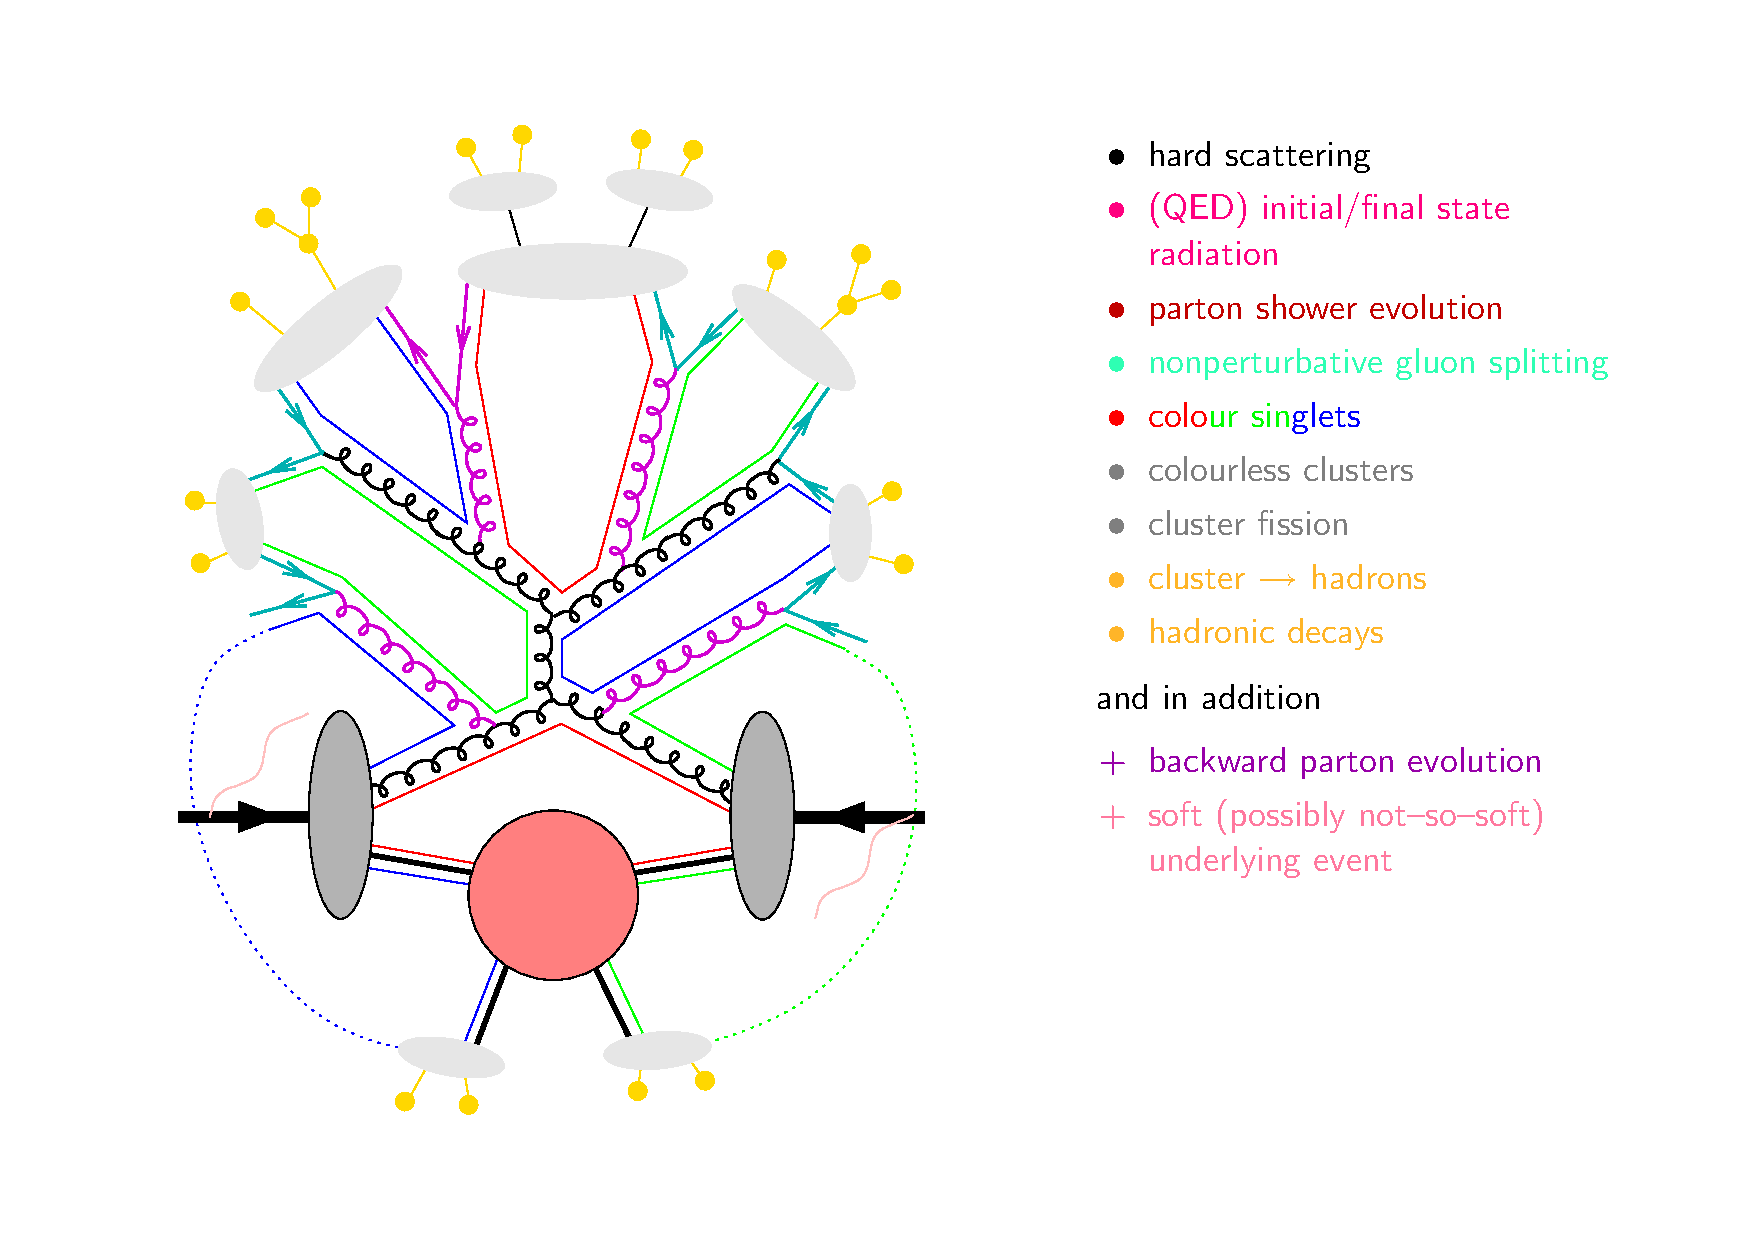
\includegraphics[width=\textwidth]{figures/Zep-soft}
\caption{An illustration of the processes that may surround an interesting event in a proton-proton collision, and the steps required to arrive at a final particle content of that event. In this figure, the dark gray blobs represent the incoming protons and the large red blob represents a hard quark-quark interaction. As illustrated here, the products of such a hard interaction may carry colour charge as well, in which case these products too would need to undergo hadronisation, which, in turn, would show up in the detector as jets. However, since the end product of the process currently under study is photons, which are colourless, that will not be the case here. The upper portion of the figure illustrates the evolution of a secondary gluon interaction, which, though a number of gluon emissions, produces a selection of quark final states that must be gathered into colourless clusters and finally into hadrons. Both stages may undergo further evolution or decay during the process. The final collection of hadrons, which will be reasonably well collimated, form a jet of particles in the detector. Similar jet-forming processes may also attach to particles emitted as initial or final state radiation. This figure reproduced from \cite{zep}. For further details on these surrounding processes and their computational representation, see eg \cite{pythman}.
\label{zep}}
\end{figure}

\section{Extended event}
The events produced by the event generator(s) represent the physical process that occurs in the point where two protons interact. Given the limits on our ability to see such interactions, we need to exptend the scope of physical processes in the simulation, to the point where the resulting event information represents something that we might realistically pick up with a detector.

The initial and final particle states are fixed in the event generator, however in reality, both initial and final states might easily undergo decay or emission before or after the event occurs, altering the particle content and kinematics of the event. Such initial and final state radiation must be modelled to give an accurate picture of what a detector might see.

Further, final state particles with colour charge will not remain isolated due to colour confinement. These particles will develop a jet of other coloured particles, so that the colour charge becomes obscured to outside observation. The simulation of the process by which colour charged particles combine into colour neutral hadrons is simulated is called hadronisation. Since we are dealing with photons in the final state in the present analysis, this step is not crucial in the events generated to study this process specifically, however $\pi^0$ mesons, one of the major backgrounds to the photon signal, are produced in this way. 

A schematic summary of these processes, along with the steps that the simulation software that models these processes will usually be divided into, is presented in figure~\ref{zep}. In this thesis, the extension of the hard events provided by CalcHEP with these surrounding processes will be carried out in pythia8 \cite{pythia}. Figure~\ref{pythify} illustrates the effect that these surrounding processes have on the distribution of invariant masses.

\begin{figure}[hbt]
\centering
\begin{minipage}[b]{.69\textwidth}\hspace{-1.5em}\makebox[0pt][l]{
\noindent\begin{infilsf}
\tiny
\pgfdeclareplotmark{cross} {
\pgfpathmoveto{\pgfpoint{-0.3\pgfplotmarksize}{\pgfplotmarksize}}
\pgfpathlineto{\pgfpoint{+0.3\pgfplotmarksize}{\pgfplotmarksize}}
\pgfpathlineto{\pgfpoint{+0.3\pgfplotmarksize}{0.3\pgfplotmarksize}}
\pgfpathlineto{\pgfpoint{+1\pgfplotmarksize}{0.3\pgfplotmarksize}}
\pgfpathlineto{\pgfpoint{+1\pgfplotmarksize}{-0.3\pgfplotmarksize}}
\pgfpathlineto{\pgfpoint{+0.3\pgfplotmarksize}{-0.3\pgfplotmarksize}}
\pgfpathlineto{\pgfpoint{+0.3\pgfplotmarksize}{-1.\pgfplotmarksize}}
\pgfpathlineto{\pgfpoint{-0.3\pgfplotmarksize}{-1.\pgfplotmarksize}}
\pgfpathlineto{\pgfpoint{-0.3\pgfplotmarksize}{-0.3\pgfplotmarksize}}
\pgfpathlineto{\pgfpoint{-1.\pgfplotmarksize}{-0.3\pgfplotmarksize}}
\pgfpathlineto{\pgfpoint{-1.\pgfplotmarksize}{0.3\pgfplotmarksize}}
\pgfpathlineto{\pgfpoint{-0.3\pgfplotmarksize}{0.3\pgfplotmarksize}}
\pgfpathclose
\pgfusepathqstroke
}
\pgfdeclareplotmark{cross*} {
\pgfpathmoveto{\pgfpoint{-0.3\pgfplotmarksize}{\pgfplotmarksize}}
\pgfpathlineto{\pgfpoint{+0.3\pgfplotmarksize}{\pgfplotmarksize}}
\pgfpathlineto{\pgfpoint{+0.3\pgfplotmarksize}{0.3\pgfplotmarksize}}
\pgfpathlineto{\pgfpoint{+1\pgfplotmarksize}{0.3\pgfplotmarksize}}
\pgfpathlineto{\pgfpoint{+1\pgfplotmarksize}{-0.3\pgfplotmarksize}}
\pgfpathlineto{\pgfpoint{+0.3\pgfplotmarksize}{-0.3\pgfplotmarksize}}
\pgfpathlineto{\pgfpoint{+0.3\pgfplotmarksize}{-1.\pgfplotmarksize}}
\pgfpathlineto{\pgfpoint{-0.3\pgfplotmarksize}{-1.\pgfplotmarksize}}
\pgfpathlineto{\pgfpoint{-0.3\pgfplotmarksize}{-0.3\pgfplotmarksize}}
\pgfpathlineto{\pgfpoint{-1.\pgfplotmarksize}{-0.3\pgfplotmarksize}}
\pgfpathlineto{\pgfpoint{-1.\pgfplotmarksize}{0.3\pgfplotmarksize}}
\pgfpathlineto{\pgfpoint{-0.3\pgfplotmarksize}{0.3\pgfplotmarksize}}
\pgfpathclose
\pgfusepathqfillstroke
}
\pgfdeclareplotmark{newstar} {
\pgfpathmoveto{\pgfqpoint{0pt}{\pgfplotmarksize}}
\pgfpathlineto{\pgfqpointpolar{44}{0.5\pgfplotmarksize}}
\pgfpathlineto{\pgfqpointpolar{18}{\pgfplotmarksize}}
\pgfpathlineto{\pgfqpointpolar{-20}{0.5\pgfplotmarksize}}
\pgfpathlineto{\pgfqpointpolar{-54}{\pgfplotmarksize}}
\pgfpathlineto{\pgfqpointpolar{-90}{0.5\pgfplotmarksize}}
\pgfpathlineto{\pgfqpointpolar{234}{\pgfplotmarksize}}
\pgfpathlineto{\pgfqpointpolar{198}{0.5\pgfplotmarksize}}
\pgfpathlineto{\pgfqpointpolar{162}{\pgfplotmarksize}}
\pgfpathlineto{\pgfqpointpolar{134}{0.5\pgfplotmarksize}}
\pgfpathclose
\pgfusepathqstroke
}
\pgfdeclareplotmark{newstar*} {
\pgfpathmoveto{\pgfqpoint{0pt}{\pgfplotmarksize}}
\pgfpathlineto{\pgfqpointpolar{44}{0.5\pgfplotmarksize}}
\pgfpathlineto{\pgfqpointpolar{18}{\pgfplotmarksize}}
\pgfpathlineto{\pgfqpointpolar{-20}{0.5\pgfplotmarksize}}
\pgfpathlineto{\pgfqpointpolar{-54}{\pgfplotmarksize}}
\pgfpathlineto{\pgfqpointpolar{-90}{0.5\pgfplotmarksize}}
\pgfpathlineto{\pgfqpointpolar{234}{\pgfplotmarksize}}
\pgfpathlineto{\pgfqpointpolar{198}{0.5\pgfplotmarksize}}
\pgfpathlineto{\pgfqpointpolar{162}{\pgfplotmarksize}}
\pgfpathlineto{\pgfqpointpolar{134}{0.5\pgfplotmarksize}}
\pgfpathclose
\pgfusepathqfillstroke
}
\begin{tikzpicture}[x=0.05\textwidth,y=.05\textwidth]

\definecolor{c}{rgb}{0,0,0};
\draw [c] (2,11.8008) -- (2,22.4216) -- (18,22.4216) -- (18,11.8008) -- (2,11.8008);

\definecolor{c}{rgb}{0,0,0};
\draw [c] (2,11.8008) -- (2,22.4216) -- (18,22.4216) -- (18,11.8008) -- (2,11.8008);
\colorlet{c}{kugray!50};
\draw [c] (2.16,22.0847) -- (2.16,22.0869);
\draw [c] (2.16,22.0869) -- (2.16,22.0891);
\draw [c] (2,22.0869) -- (2.16,22.0869);
\draw [c] (2.16,22.0869) -- (2.32,22.0869);
\draw [c] (2.48,20.989) -- (2.48,20.9954);
\draw [c] (2.48,20.9954) -- (2.48,21.0016);
\draw [c] (2.32,20.9954) -- (2.48,20.9954);
\draw [c] (2.48,20.9954) -- (2.64,20.9954);
\draw [c] (2.8,20.2777) -- (2.8,20.2902);
\draw [c] (2.8,20.2902) -- (2.8,20.3024);
\draw [c] (2.64,20.2902) -- (2.8,20.2902);
\draw [c] (2.8,20.2902) -- (2.96,20.2902);
\draw [c] (3.12,19.7357) -- (3.12,19.7568);
\draw [c] (3.12,19.7568) -- (3.12,19.777);
\draw [c] (2.96,19.7568) -- (3.12,19.7568);
\draw [c] (3.12,19.7568) -- (3.28,19.7568);
\draw [c] (3.44,19.2804) -- (3.44,19.313);
\draw [c] (3.44,19.313) -- (3.44,19.3436);
\draw [c] (3.28,19.313) -- (3.44,19.313);
\draw [c] (3.44,19.313) -- (3.6,19.313);
\draw [c] (3.76,18.9425) -- (3.76,18.9876);
\draw [c] (3.76,18.9876) -- (3.76,19.0291);
\draw [c] (3.6,18.9876) -- (3.76,18.9876);
\draw [c] (3.76,18.9876) -- (3.92,18.9876);
\draw [c] (4.08,18.4927) -- (4.08,18.5621);
\draw [c] (4.08,18.5621) -- (4.08,18.6234);
\draw [c] (3.92,18.5621) -- (4.08,18.5621);
\draw [c] (4.08,18.5621) -- (4.24,18.5621);
\draw [c] (4.4,18.1352) -- (4.4,18.2331);
\draw [c] (4.4,18.2331) -- (4.4,18.3154);
\draw [c] (4.24,18.2331) -- (4.4,18.2331);
\draw [c] (4.4,18.2331) -- (4.56,18.2331);
\draw [c] (4.72,17.8253) -- (4.72,17.957);
\draw [c] (4.72,17.957) -- (4.72,18.062);
\draw [c] (4.56,17.957) -- (4.72,17.957);
\draw [c] (4.72,17.957) -- (4.88,17.957);
\draw [c] (5.04,17.7645) -- (5.04,17.8494);
\draw [c] (5.04,17.8494) -- (5.04,17.9225);
\draw [c] (4.88,17.8494) -- (5.04,17.8494);
\draw [c] (5.04,17.8494) -- (5.2,17.8494);
\draw [c] (5.36,17.4837) -- (5.36,17.4878);
\draw [c] (5.36,17.4878) -- (5.36,17.4919);
\draw [c] (5.2,17.4878) -- (5.36,17.4878);
\draw [c] (5.36,17.4878) -- (5.52,17.4878);
\draw [c] (5.68,17.2475) -- (5.68,17.2526);
\draw [c] (5.68,17.2526) -- (5.68,17.2577);
\draw [c] (5.52,17.2526) -- (5.68,17.2526);
\draw [c] (5.68,17.2526) -- (5.84,17.2526);
\draw [c] (6,16.9982) -- (6,17.0047);
\draw [c] (6,17.0047) -- (6,17.0112);
\draw [c] (5.84,17.0047) -- (6,17.0047);
\draw [c] (6,17.0047) -- (6.16,17.0047);
\draw [c] (6.32,16.7792) -- (6.32,16.7873);
\draw [c] (6.32,16.7873) -- (6.32,16.7952);
\draw [c] (6.16,16.7873) -- (6.32,16.7873);
\draw [c] (6.32,16.7873) -- (6.48,16.7873);
\draw [c] (6.64,16.5651) -- (6.64,16.575);
\draw [c] (6.64,16.575) -- (6.64,16.5847);
\draw [c] (6.48,16.575) -- (6.64,16.575);
\draw [c] (6.64,16.575) -- (6.8,16.575);
\draw [c] (6.96,16.3657) -- (6.96,16.3776);
\draw [c] (6.96,16.3776) -- (6.96,16.3893);
\draw [c] (6.8,16.3776) -- (6.96,16.3776);
\draw [c] (6.96,16.3776) -- (7.12,16.3776);
\draw [c] (7.28,16.1641) -- (7.28,16.1786);
\draw [c] (7.28,16.1786) -- (7.28,16.1927);
\draw [c] (7.12,16.1786) -- (7.28,16.1786);
\draw [c] (7.28,16.1786) -- (7.44,16.1786);
\draw [c] (7.6,15.9868) -- (7.6,16.004);
\draw [c] (7.6,16.004) -- (7.6,16.0206);
\draw [c] (7.44,16.004) -- (7.6,16.004);
\draw [c] (7.6,16.004) -- (7.76,16.004);
\draw [c] (7.92,15.7677) -- (7.92,15.7889);
\draw [c] (7.92,15.7889) -- (7.92,15.8093);
\draw [c] (7.76,15.7889) -- (7.92,15.7889);
\draw [c] (7.92,15.7889) -- (8.08,15.7889);
\draw [c] (8.24,15.4855) -- (8.24,15.5133);
\draw [c] (8.24,15.5133) -- (8.24,15.5398);
\draw [c] (8.08,15.5133) -- (8.24,15.5133);
\draw [c] (8.24,15.5133) -- (8.4,15.5133);
\draw [c] (8.56,15.2517) -- (8.56,15.2866);
\draw [c] (8.56,15.2866) -- (8.56,15.3193);
\draw [c] (8.4,15.2866) -- (8.56,15.2866);
\draw [c] (8.56,15.2866) -- (8.72,15.2866);
\draw [c] (8.88,14.9685) -- (8.88,15.0142);
\draw [c] (8.88,15.0142) -- (8.88,15.0563);
\draw [c] (8.72,15.0142) -- (8.88,15.0142);
\draw [c] (8.88,15.0142) -- (9.04,15.0142);
\draw [c] (9.2,14.9072) -- (9.2,14.9557);
\draw [c] (9.2,14.9557) -- (9.2,15.0001);
\draw [c] (9.04,14.9557) -- (9.2,14.9557);
\draw [c] (9.2,14.9557) -- (9.36,14.9557);
\draw [c] (9.52,14.6847) -- (9.52,14.7448);
\draw [c] (9.52,14.7448) -- (9.52,14.7987);
\draw [c] (9.36,14.7448) -- (9.52,14.7448);
\draw [c] (9.52,14.7448) -- (9.68,14.7448);
\draw [c] (9.84,14.3956) -- (9.84,14.4749);
\draw [c] (9.84,14.4749) -- (9.84,14.5437);
\draw [c] (9.68,14.4749) -- (9.84,14.4749);
\draw [c] (9.84,14.4749) -- (10,14.4749);
\draw [c] (10.16,14.24) -- (10.16,14.3321);
\draw [c] (10.16,14.3321) -- (10.16,14.4103);
\draw [c] (10,14.3321) -- (10.16,14.3321);
\draw [c] (10.16,14.3321) -- (10.32,14.3321);
\draw [c] (10.48,13.9492) -- (10.48,14.0709);
\draw [c] (10.48,14.0709) -- (10.48,14.1694);
\draw [c] (10.32,14.0709) -- (10.48,14.0709);
\draw [c] (10.48,14.0709) -- (10.64,14.0709);
\draw [c] (10.8,13.923) -- (10.8,14.0478);
\draw [c] (10.8,14.0478) -- (10.8,14.1483);
\draw [c] (10.64,14.0478) -- (10.8,14.0478);
\draw [c] (10.8,14.0478) -- (10.96,14.0478);
\draw [c] (11.12,13.6051) -- (11.12,13.7741);
\draw [c] (11.12,13.7741) -- (11.12,13.9014);
\draw [c] (10.96,13.7741) -- (11.12,13.7741);
\draw [c] (11.12,13.7741) -- (11.28,13.7741);
\draw [c] (11.44,13.5552) -- (11.44,13.7324);
\draw [c] (11.44,13.7324) -- (11.44,13.8644);
\draw [c] (11.28,13.7324) -- (11.44,13.7324);
\draw [c] (11.44,13.7324) -- (11.6,13.7324);
\draw [c] (11.76,13.5005) -- (11.76,13.6872);
\draw [c] (11.76,13.6872) -- (11.76,13.8243);
\draw [c] (11.6,13.6872) -- (11.76,13.6872);
\draw [c] (11.76,13.6872) -- (11.92,13.6872);
\draw [c] (12.08,12.8003) -- (12.08,13.1609);
\draw [c] (12.08,13.1609) -- (12.08,13.3718);
\draw [c] (11.92,13.1609) -- (12.08,13.1609);
\draw [c] (12.08,13.1609) -- (12.24,13.1609);
\draw [c] (12.4,13.5005) -- (12.4,13.6872);
\draw [c] (12.4,13.6872) -- (12.4,13.8243);
\draw [c] (12.24,13.6872) -- (12.4,13.6872);
\draw [c] (12.4,13.6872) -- (12.56,13.6872);
\draw [c] (12.72,11.8008) -- (12.72,12.4397);
\draw [c] (12.72,12.4397) -- (12.72,12.8003);
\draw [c] (12.56,12.4397) -- (12.72,12.4397);
\draw [c] (12.72,12.4397) -- (12.88,12.4397);
\draw [c] (13.04,11.8008) -- (13.04,12.4397);
\draw [c] (13.04,12.4397) -- (13.04,12.8003);
\draw [c] (12.88,12.4397) -- (13.04,12.4397);
\draw [c] (13.04,12.4397) -- (13.2,12.4397);
\draw [c] (13.36,11.8008) -- (13.36,12.4397);
\draw [c] (13.36,12.4397) -- (13.36,12.8003);
\draw [c] (13.2,12.4397) -- (13.36,12.4397);
\draw [c] (13.36,12.4397) -- (13.52,12.4397);
\draw [c] (13.68,12.1614) -- (13.68,12.8003);
\draw [c] (13.68,12.8003) -- (13.68,13.0785);
\draw [c] (13.52,12.8003) -- (13.68,12.8003);
\draw [c] (13.68,12.8003) -- (13.84,12.8003);
\draw [c] (14,11.8008) -- (14,12.4397);
\draw [c] (14,12.4397) -- (14,12.8003);
\draw [c] (13.84,12.4397) -- (14,12.4397);
\draw [c] (14,12.4397) -- (14.16,12.4397);
\draw [c] (14.32,11.8008) -- (14.32,12.4397);
\draw [c] (14.32,12.4397) -- (14.32,12.8003);
\draw [c] (14.16,12.4397) -- (14.32,12.4397);
\draw [c] (14.32,12.4397) -- (14.48,12.4397);
\draw [c] (14.64,11.8008) -- (14.64,12.4397);
\draw [c] (14.64,12.4397) -- (14.64,12.8003);
\draw [c] (14.48,12.4397) -- (14.64,12.4397);
\draw [c] (14.64,12.4397) -- (14.8,12.4397);
\draw [c] (15.28,11.8008) -- (15.28,12.4397);
\draw [c] (15.28,12.4397) -- (15.28,12.8003);
\draw [c] (15.12,12.4397) -- (15.28,12.4397);
\draw [c] (15.28,12.4397) -- (15.44,12.4397);
\definecolor{c}{rgb}{0,0,0};
\draw [c] (2,11.8008) -- (18,11.8008);
\draw [c] (3.30612,12.084) -- (3.30612,11.8008);
\draw [c] (3.63265,11.9424) -- (3.63265,11.8008);
\draw [c] (3.95918,11.9424) -- (3.95918,11.8008);
\draw [c] (4.28571,11.9424) -- (4.28571,11.8008);
\draw [c] (4.61225,11.9424) -- (4.61225,11.8008);
\draw [c] (4.93878,12.084) -- (4.93878,11.8008);
\draw [c] (5.26531,11.9424) -- (5.26531,11.8008);
\draw [c] (5.59184,11.9424) -- (5.59184,11.8008);
\draw [c] (5.91837,11.9424) -- (5.91837,11.8008);
\draw [c] (6.2449,11.9424) -- (6.2449,11.8008);
\draw [c] (6.57143,12.084) -- (6.57143,11.8008);
\draw [c] (6.89796,11.9424) -- (6.89796,11.8008);
\draw [c] (7.22449,11.9424) -- (7.22449,11.8008);
\draw [c] (7.55102,11.9424) -- (7.55102,11.8008);
\draw [c] (7.87755,11.9424) -- (7.87755,11.8008);
\draw [c] (8.20408,12.084) -- (8.20408,11.8008);
\draw [c] (8.53061,11.9424) -- (8.53061,11.8008);
\draw [c] (8.85714,11.9424) -- (8.85714,11.8008);
\draw [c] (9.18367,11.9424) -- (9.18367,11.8008);
\draw [c] (9.5102,11.9424) -- (9.5102,11.8008);
\draw [c] (9.83673,12.084) -- (9.83673,11.8008);
\draw [c] (10.1633,11.9424) -- (10.1633,11.8008);
\draw [c] (10.4898,11.9424) -- (10.4898,11.8008);
\draw [c] (10.8163,11.9424) -- (10.8163,11.8008);
\draw [c] (11.1429,11.9424) -- (11.1429,11.8008);
\draw [c] (11.4694,12.084) -- (11.4694,11.8008);
\draw [c] (11.7959,11.9424) -- (11.7959,11.8008);
\draw [c] (12.1224,11.9424) -- (12.1224,11.8008);
\draw [c] (12.449,11.9424) -- (12.449,11.8008);
\draw [c] (12.7755,11.9424) -- (12.7755,11.8008);
\draw [c] (13.102,12.084) -- (13.102,11.8008);
\draw [c] (13.4286,11.9424) -- (13.4286,11.8008);
\draw [c] (13.7551,11.9424) -- (13.7551,11.8008);
\draw [c] (14.0816,11.9424) -- (14.0816,11.8008);
\draw [c] (14.4082,11.9424) -- (14.4082,11.8008);
\draw [c] (14.7347,12.084) -- (14.7347,11.8008);
\draw [c] (15.0612,11.9424) -- (15.0612,11.8008);
\draw [c] (15.3878,11.9424) -- (15.3878,11.8008);
\draw [c] (15.7143,11.9424) -- (15.7143,11.8008);
\draw [c] (16.0408,11.9424) -- (16.0408,11.8008);
\draw [c] (16.3673,12.084) -- (16.3673,11.8008);
\draw [c] (16.6939,11.9424) -- (16.6939,11.8008);
\draw [c] (17.0204,11.9424) -- (17.0204,11.8008);
\draw [c] (17.3469,11.9424) -- (17.3469,11.8008);
\draw [c] (17.6735,11.9424) -- (17.6735,11.8008);
\draw [c] (18,12.084) -- (18,11.8008);
\draw [c] (3.30612,12.084) -- (3.30612,11.8008);
\draw [c] (2.97959,11.9424) -- (2.97959,11.8008);
\draw [c] (2.65306,11.9424) -- (2.65306,11.8008);
\draw [c] (2.32653,11.9424) -- (2.32653,11.8008);

\draw [c] (2,11.8008) -- (2,22.4216);
\draw [anchor= east] (0.1,22.4216) node[ rotate=90]{$\di\sigma/\di M_{\gamma\gamma}$ [pb/GeV]};
\draw [c] (2.27,11.8185) -- (2,11.8185);
\draw [c] (2.27,11.8986) -- (2,11.8986);
\draw [c] (2.27,11.9681) -- (2,11.9681);
\draw [c] (2.27,12.0294) -- (2,12.0294);
\draw [c] (2.54,12.0842) -- (2,12.0842);
\draw [anchor= east] (1.844,12.0842) node[ rotate=0]{$10^{-10}$};
\draw [c] (2.27,12.4448) -- (2,12.4448);
\draw [c] (2.27,12.6558) -- (2,12.6558);
\draw [c] (2.27,12.8054) -- (2,12.8054);
\draw [c] (2.27,12.9215) -- (2,12.9215);
\draw [c] (2.27,13.0164) -- (2,13.0164);
\draw [c] (2.27,13.0966) -- (2,13.0966);
\draw [c] (2.27,13.166) -- (2,13.166);
\draw [c] (2.27,13.2273) -- (2,13.2273);
\draw [c] (2.54,13.2821) -- (2,13.2821);
\draw [anchor= east] (1.844,13.2821) node[ rotate=0]{$10^{-9}$};
\draw [c] (2.27,13.6427) -- (2,13.6427);
\draw [c] (2.27,13.8537) -- (2,13.8537);
\draw [c] (2.27,14.0033) -- (2,14.0033);
\draw [c] (2.27,14.1194) -- (2,14.1194);
\draw [c] (2.27,14.2143) -- (2,14.2143);
\draw [c] (2.27,14.2945) -- (2,14.2945);
\draw [c] (2.27,14.364) -- (2,14.364);
\draw [c] (2.27,14.4252) -- (2,14.4252);
\draw [c] (2.54,14.48) -- (2,14.48);
\draw [anchor= east] (1.844,14.48) node[ rotate=0]{$10^{-8}$};
\draw [c] (2.27,14.8407) -- (2,14.8407);
\draw [c] (2.27,15.0516) -- (2,15.0516);
\draw [c] (2.27,15.2013) -- (2,15.2013);
\draw [c] (2.27,15.3174) -- (2,15.3174);
\draw [c] (2.27,15.4122) -- (2,15.4122);
\draw [c] (2.27,15.4924) -- (2,15.4924);
\draw [c] (2.27,15.5619) -- (2,15.5619);
\draw [c] (2.27,15.6231) -- (2,15.6231);
\draw [c] (2.54,15.678) -- (2,15.678);
\draw [anchor= east] (1.844,15.678) node[ rotate=0]{$10^{-7}$};
\draw [c] (2.27,16.0386) -- (2,16.0386);
\draw [c] (2.27,16.2495) -- (2,16.2495);
\draw [c] (2.27,16.3992) -- (2,16.3992);
\draw [c] (2.27,16.5153) -- (2,16.5153);
\draw [c] (2.27,16.6101) -- (2,16.6101);
\draw [c] (2.27,16.6903) -- (2,16.6903);
\draw [c] (2.27,16.7598) -- (2,16.7598);
\draw [c] (2.27,16.8211) -- (2,16.8211);
\draw [c] (2.54,16.8759) -- (2,16.8759);
\draw [anchor= east] (1.844,16.8759) node[ rotate=0]{$10^{-6}$};
\draw [c] (2.27,17.2365) -- (2,17.2365);
\draw [c] (2.27,17.4474) -- (2,17.4474);
\draw [c] (2.27,17.5971) -- (2,17.5971);
\draw [c] (2.27,17.7132) -- (2,17.7132);
\draw [c] (2.27,17.808) -- (2,17.808);
\draw [c] (2.27,17.8882) -- (2,17.8882);
\draw [c] (2.27,17.9577) -- (2,17.9577);
\draw [c] (2.27,18.019) -- (2,18.019);
\draw [c] (2.54,18.0738) -- (2,18.0738);
\draw [anchor= east] (1.844,18.0738) node[ rotate=0]{$10^{-5}$};
\draw [c] (2.27,18.4344) -- (2,18.4344);
\draw [c] (2.27,18.6453) -- (2,18.6453);
\draw [c] (2.27,18.795) -- (2,18.795);
\draw [c] (2.27,18.9111) -- (2,18.9111);
\draw [c] (2.27,19.006) -- (2,19.006);
\draw [c] (2.27,19.0861) -- (2,19.0861);
\draw [c] (2.27,19.1556) -- (2,19.1556);
\draw [c] (2.27,19.2169) -- (2,19.2169);
\draw [c] (2.54,19.2717) -- (2,19.2717);
\draw [anchor= east] (1.844,19.2717) node[ rotate=0]{$10^{-4}$};
\draw [c] (2.27,19.6323) -- (2,19.6323);
\draw [c] (2.27,19.8433) -- (2,19.8433);
\draw [c] (2.27,19.9929) -- (2,19.9929);
\draw [c] (2.27,20.109) -- (2,20.109);
\draw [c] (2.27,20.2039) -- (2,20.2039);
\draw [c] (2.27,20.2841) -- (2,20.2841);
\draw [c] (2.27,20.3535) -- (2,20.3535);
\draw [c] (2.27,20.4148) -- (2,20.4148);
\draw [c] (2.54,20.4696) -- (2,20.4696);
\draw [anchor= east] (1.844,20.4696) node[ rotate=0]{$10^{-3}$};
\draw [c] (2.27,20.8302) -- (2,20.8302);
\draw [c] (2.27,21.0412) -- (2,21.0412);
\draw [c] (2.27,21.1908) -- (2,21.1908);
\draw [c] (2.27,21.3069) -- (2,21.3069);
\draw [c] (2.27,21.4018) -- (2,21.4018);
\draw [c] (2.27,21.482) -- (2,21.482);
\draw [c] (2.27,21.5515) -- (2,21.5515);
\draw [c] (2.27,21.6127) -- (2,21.6127);
\draw [c] (2.54,21.6675) -- (2,21.6675);
\draw [anchor= east] (1.844,21.6675) node[ rotate=0]{$10^{-2}$};
\draw [c] (2.27,22.0282) -- (2,22.0282);
\draw [c] (2.27,22.2391) -- (2,22.2391);
\draw [c] (2.27,22.3888) -- (2,22.3888);
\colorlet{c}{kugray};
\draw [c] (2.16,21.9886) -- (2.16,21.9911);
\draw [c] (2.16,21.9911) -- (2.16,21.9935);
\draw [c] (2,21.9911) -- (2.16,21.9911);
\draw [c] (2.16,21.9911) -- (2.32,21.9911);
\draw [c] (2.48,20.8999) -- (2.48,20.9067);
\draw [c] (2.48,20.9067) -- (2.48,20.9135);
\draw [c] (2.32,20.9067) -- (2.48,20.9067);
\draw [c] (2.48,20.9067) -- (2.64,20.9067);
\draw [c] (2.8,20.1651) -- (2.8,20.179);
\draw [c] (2.8,20.179) -- (2.8,20.1926);
\draw [c] (2.64,20.179) -- (2.8,20.179);
\draw [c] (2.8,20.179) -- (2.96,20.179);
\draw [c] (3.12,19.6256) -- (3.12,19.649);
\draw [c] (3.12,19.649) -- (3.12,19.6714);
\draw [c] (2.96,19.649) -- (3.12,19.649);
\draw [c] (3.12,19.649) -- (3.28,19.649);
\draw [c] (3.44,19.2037) -- (3.44,19.2388);
\draw [c] (3.44,19.2388) -- (3.44,19.2717);
\draw [c] (3.28,19.2388) -- (3.44,19.2388);
\draw [c] (3.44,19.2388) -- (3.6,19.2388);
\draw [c] (3.76,18.8394) -- (3.76,18.8892);
\draw [c] (3.76,18.8892) -- (3.76,18.9346);
\draw [c] (3.6,18.8892) -- (3.76,18.8892);
\draw [c] (3.76,18.8892) -- (3.92,18.8892);
\draw [c] (4.08,18.3977) -- (4.08,18.4738);
\draw [c] (4.08,18.4738) -- (4.08,18.5401);
\draw [c] (3.92,18.4738) -- (4.08,18.4738);
\draw [c] (4.08,18.4738) -- (4.24,18.4738);
\draw [c] (4.4,18.0231) -- (4.4,18.1321);
\draw [c] (4.4,18.1321) -- (4.4,18.2221);
\draw [c] (4.24,18.1321) -- (4.4,18.1321);
\draw [c] (4.4,18.1321) -- (4.56,18.1321);
\draw [c] (4.72,17.5639) -- (4.72,17.7329);
\draw [c] (4.72,17.7329) -- (4.72,17.8603);
\draw [c] (4.56,17.7329) -- (4.72,17.7329);
\draw [c] (4.72,17.7329) -- (4.88,17.7329);
\draw [c] (5.04,17.6487) -- (5.04,17.7446);
\draw [c] (5.04,17.7446) -- (5.04,17.8255);
\draw [c] (4.88,17.7446) -- (5.04,17.7446);
\draw [c] (5.04,17.7446) -- (5.2,17.7446);
\draw [c] (5.36,17.3748) -- (5.36,17.3793);
\draw [c] (5.36,17.3793) -- (5.36,17.3838);
\draw [c] (5.2,17.3793) -- (5.36,17.3793);
\draw [c] (5.36,17.3793) -- (5.52,17.3793);
\draw [c] (5.68,17.1419) -- (5.68,17.1476);
\draw [c] (5.68,17.1476) -- (5.68,17.1532);
\draw [c] (5.52,17.1476) -- (5.68,17.1476);
\draw [c] (5.68,17.1476) -- (5.84,17.1476);
\draw [c] (6,16.8903) -- (6,16.8975);
\draw [c] (6,16.8975) -- (6,16.9046);
\draw [c] (5.84,16.8975) -- (6,16.8975);
\draw [c] (6,16.8975) -- (6.16,16.8975);
\draw [c] (6.32,16.6718) -- (6.32,16.6807);
\draw [c] (6.32,16.6807) -- (6.32,16.6894);
\draw [c] (6.16,16.6807) -- (6.32,16.6807);
\draw [c] (6.32,16.6807) -- (6.48,16.6807);
\draw [c] (6.64,16.4482) -- (6.64,16.4592);
\draw [c] (6.64,16.4592) -- (6.64,16.47);
\draw [c] (6.48,16.4592) -- (6.64,16.4592);
\draw [c] (6.64,16.4592) -- (6.8,16.4592);
\draw [c] (6.96,16.2518) -- (6.96,16.2651);
\draw [c] (6.96,16.2651) -- (6.96,16.2781);
\draw [c] (6.8,16.2651) -- (6.96,16.2651);
\draw [c] (6.96,16.2651) -- (7.12,16.2651);
\draw [c] (7.28,16.043) -- (7.28,16.0593);
\draw [c] (7.28,16.0593) -- (7.28,16.0751);
\draw [c] (7.12,16.0593) -- (7.28,16.0593);
\draw [c] (7.28,16.0593) -- (7.44,16.0593);
\draw [c] (7.6,15.8872) -- (7.6,15.9061);
\draw [c] (7.6,15.9061) -- (7.6,15.9244);
\draw [c] (7.44,15.9061) -- (7.6,15.9061);
\draw [c] (7.6,15.9061) -- (7.76,15.9061);
\draw [c] (7.92,15.6564) -- (7.92,15.68);
\draw [c] (7.92,15.68) -- (7.92,15.7026);
\draw [c] (7.76,15.68) -- (7.92,15.68);
\draw [c] (7.92,15.68) -- (8.08,15.68);
\draw [c] (8.24,15.3725) -- (8.24,15.4036);
\draw [c] (8.24,15.4036) -- (8.24,15.4329);
\draw [c] (8.08,15.4036) -- (8.24,15.4036);
\draw [c] (8.24,15.4036) -- (8.4,15.4036);
\draw [c] (8.56,15.1099) -- (8.56,15.1499);
\draw [c] (8.56,15.1499) -- (8.56,15.187);
\draw [c] (8.4,15.1499) -- (8.56,15.1499);
\draw [c] (8.56,15.1499) -- (8.72,15.1499);
\draw [c] (8.88,14.862) -- (8.88,14.9127);
\draw [c] (8.88,14.9127) -- (8.88,14.9589);
\draw [c] (8.72,14.9127) -- (8.88,14.9127);
\draw [c] (8.88,14.9127) -- (9.04,14.9127);
\draw [c] (9.2,14.8126) -- (9.2,14.8658);
\draw [c] (9.2,14.8658) -- (9.2,14.914);
\draw [c] (9.04,14.8658) -- (9.2,14.8658);
\draw [c] (9.2,14.8658) -- (9.36,14.8658);
\draw [c] (9.52,14.5837) -- (9.52,14.6499);
\draw [c] (9.52,14.6499) -- (9.52,14.7087);
\draw [c] (9.36,14.6499) -- (9.52,14.6499);
\draw [c] (9.52,14.6499) -- (9.68,14.6499);
\draw [c] (9.84,14.2548) -- (9.84,14.3456);
\draw [c] (9.84,14.3456) -- (9.84,14.4229);
\draw [c] (9.68,14.3456) -- (9.84,14.3456);
\draw [c] (9.84,14.3456) -- (10,14.3456);
\draw [c] (10.16,14.1042) -- (10.16,14.2091);
\draw [c] (10.16,14.2091) -- (10.16,14.2964);
\draw [c] (10,14.2091) -- (10.16,14.2091);
\draw [c] (10.16,14.2091) -- (10.32,14.2091);
\draw [c] (10.48,13.7691) -- (10.48,13.9136);
\draw [c] (10.48,13.9136) -- (10.48,14.0266);
\draw [c] (10.32,13.9136) -- (10.48,13.9136);
\draw [c] (10.48,13.9136) -- (10.64,13.9136);
\draw [c] (10.8,13.7691) -- (10.8,13.9136);
\draw [c] (10.8,13.9136) -- (10.8,14.0266);
\draw [c] (10.64,13.9136) -- (10.8,13.9136);
\draw [c] (10.8,13.9136) -- (10.96,13.9136);
\draw [c] (11.12,13.5005) -- (11.12,13.6872);
\draw [c] (11.12,13.6872) -- (11.12,13.8243);
\draw [c] (10.96,13.6872) -- (11.12,13.6872);
\draw [c] (11.12,13.6872) -- (11.28,13.6872);
\draw [c] (11.44,13.4398) -- (11.44,13.6376);
\draw [c] (11.44,13.6376) -- (11.44,13.7805);
\draw [c] (11.28,13.6376) -- (11.44,13.6376);
\draw [c] (11.44,13.6376) -- (11.6,13.6376);
\draw [c] (11.76,13.3718) -- (11.76,13.5828);
\draw [c] (11.76,13.5828) -- (11.76,13.7324);
\draw [c] (11.6,13.5828) -- (11.76,13.5828);
\draw [c] (11.76,13.5828) -- (11.92,13.5828);
\draw [c] (12.08,12.1614) -- (12.08,12.8003);
\draw [c] (12.08,12.8003) -- (12.08,13.0785);
\draw [c] (11.92,12.8003) -- (12.08,12.8003);
\draw [c] (12.08,12.8003) -- (12.24,12.8003);
\draw [c] (12.4,13.4398) -- (12.4,13.6376);
\draw [c] (12.4,13.6376) -- (12.4,13.7805);
\draw [c] (12.24,13.6376) -- (12.4,13.6376);
\draw [c] (12.4,13.6376) -- (12.56,13.6376);
\draw [c] (13.04,11.8008) -- (13.04,12.4397);
\draw [c] (13.04,12.4397) -- (13.04,12.8003);
\draw [c] (12.88,12.4397) -- (13.04,12.4397);
\draw [c] (13.04,12.4397) -- (13.2,12.4397);
\draw [c] (13.36,11.8008) -- (13.36,12.4397);
\draw [c] (13.36,12.4397) -- (13.36,12.8003);
\draw [c] (13.2,12.4397) -- (13.36,12.4397);
\draw [c] (13.36,12.4397) -- (13.52,12.4397);
\draw [c] (13.68,11.8008) -- (13.68,12.4397);
\draw [c] (13.68,12.4397) -- (13.68,12.8003);
\draw [c] (13.52,12.4397) -- (13.68,12.4397);
\draw [c] (13.68,12.4397) -- (13.84,12.4397);
\colorlet{c}{natgreen!50};
\draw [c] (2.16,22.0854) -- (2.16,22.0876);
\draw [c] (2.16,22.0876) -- (2.16,22.0898);
\draw [c] (2,22.0876) -- (2.16,22.0876);
\draw [c] (2.16,22.0876) -- (2.32,22.0876);
\draw [c] (2.48,21.0058) -- (2.48,21.012);
\draw [c] (2.48,21.012) -- (2.48,21.0181);
\draw [c] (2.32,21.012) -- (2.48,21.012);
\draw [c] (2.48,21.012) -- (2.64,21.012);
\draw [c] (2.8,20.2599) -- (2.8,20.2726);
\draw [c] (2.8,20.2726) -- (2.8,20.2851);
\draw [c] (2.64,20.2726) -- (2.8,20.2726);
\draw [c] (2.8,20.2726) -- (2.96,20.2726);
\draw [c] (3.12,19.7099) -- (3.12,19.7315);
\draw [c] (3.12,19.7315) -- (3.12,19.7522);
\draw [c] (2.96,19.7315) -- (3.12,19.7315);
\draw [c] (3.12,19.7315) -- (3.28,19.7315);
\draw [c] (3.44,19.3211) -- (3.44,19.3525);
\draw [c] (3.44,19.3525) -- (3.44,19.3821);
\draw [c] (3.28,19.3525) -- (3.44,19.3525);
\draw [c] (3.44,19.3525) -- (3.6,19.3525);
\draw [c] (3.76,18.928) -- (3.76,18.9738);
\draw [c] (3.76,18.9738) -- (3.76,19.0158);
\draw [c] (3.6,18.9738) -- (3.76,18.9738);
\draw [c] (3.76,18.9738) -- (3.92,18.9738);
\draw [c] (4.08,18.5665) -- (4.08,18.6313);
\draw [c] (4.08,18.6313) -- (4.08,18.6889);
\draw [c] (3.92,18.6313) -- (4.08,18.6313);
\draw [c] (4.08,18.6313) -- (4.24,18.6313);
\draw [c] (4.4,18.2956) -- (4.4,18.3796);
\draw [c] (4.4,18.3796) -- (4.4,18.4519);
\draw [c] (4.24,18.3796) -- (4.4,18.3796);
\draw [c] (4.4,18.3796) -- (4.56,18.3796);
\draw [c] (4.72,18.0441) -- (4.72,18.151);
\draw [c] (4.72,18.151) -- (4.72,18.2396);
\draw [c] (4.56,18.151) -- (4.72,18.151);
\draw [c] (4.72,18.151) -- (4.88,18.151);
\draw [c] (5.04,17.8055) -- (5.04,17.8627);
\draw [c] (5.04,17.8627) -- (5.04,17.9143);
\draw [c] (4.88,17.8627) -- (5.04,17.8627);
\draw [c] (5.04,17.8627) -- (5.2,17.8627);
\draw [c] (5.36,17.6929) -- (5.36,17.6978);
\draw [c] (5.36,17.6978) -- (5.36,17.7026);
\draw [c] (5.2,17.6978) -- (5.36,17.6978);
\draw [c] (5.36,17.6978) -- (5.52,17.6978);
\draw [c] (5.68,17.5229) -- (5.68,17.5286);
\draw [c] (5.68,17.5286) -- (5.68,17.5343);
\draw [c] (5.52,17.5286) -- (5.68,17.5286);
\draw [c] (5.68,17.5286) -- (5.84,17.5286);
\draw [c] (6,17.3746) -- (6,17.3812);
\draw [c] (6,17.3812) -- (6,17.3877);
\draw [c] (5.84,17.3812) -- (6,17.3812);
\draw [c] (6,17.3812) -- (6.16,17.3812);
\draw [c] (6.32,17.2692) -- (6.32,17.2765);
\draw [c] (6.32,17.2765) -- (6.32,17.2837);
\draw [c] (6.16,17.2765) -- (6.32,17.2765);
\draw [c] (6.32,17.2765) -- (6.48,17.2765);
\draw [c] (6.64,17.1541) -- (6.64,17.1623);
\draw [c] (6.64,17.1623) -- (6.64,17.1703);
\draw [c] (6.48,17.1623) -- (6.64,17.1623);
\draw [c] (6.64,17.1623) -- (6.8,17.1623);
\draw [c] (6.96,17.0606) -- (6.96,17.0695);
\draw [c] (6.96,17.0695) -- (6.96,17.0783);
\draw [c] (6.8,17.0695) -- (6.96,17.0695);
\draw [c] (6.96,17.0695) -- (7.12,17.0695);
\draw [c] (7.28,16.9827) -- (7.28,16.9923);
\draw [c] (7.28,16.9923) -- (7.28,17.0018);
\draw [c] (7.12,16.9923) -- (7.28,16.9923);
\draw [c] (7.28,16.9923) -- (7.44,16.9923);
\draw [c] (7.6,16.9271) -- (7.6,16.9372);
\draw [c] (7.6,16.9372) -- (7.6,16.9472);
\draw [c] (7.44,16.9372) -- (7.6,16.9372);
\draw [c] (7.6,16.9372) -- (7.76,16.9372);
\draw [c] (7.92,16.8537) -- (7.92,16.8646);
\draw [c] (7.92,16.8646) -- (7.92,16.8752);
\draw [c] (7.76,16.8646) -- (7.92,16.8646);
\draw [c] (7.92,16.8646) -- (8.08,16.8646);
\draw [c] (8.24,16.8089) -- (8.24,16.8203);
\draw [c] (8.24,16.8203) -- (8.24,16.8314);
\draw [c] (8.08,16.8203) -- (8.24,16.8203);
\draw [c] (8.24,16.8203) -- (8.4,16.8203);
\draw [c] (8.56,16.7645) -- (8.56,16.7764);
\draw [c] (8.56,16.7764) -- (8.56,16.788);
\draw [c] (8.4,16.7764) -- (8.56,16.7764);
\draw [c] (8.56,16.7764) -- (8.72,16.7764);
\draw [c] (8.88,16.7259) -- (8.88,16.7382);
\draw [c] (8.88,16.7382) -- (8.88,16.7502);
\draw [c] (8.72,16.7382) -- (8.88,16.7382);
\draw [c] (8.88,16.7382) -- (9.04,16.7382);
\draw [c] (9.2,16.6876) -- (9.2,16.7004);
\draw [c] (9.2,16.7004) -- (9.2,16.7129);
\draw [c] (9.04,16.7004) -- (9.2,16.7004);
\draw [c] (9.2,16.7004) -- (9.36,16.7004);
\draw [c] (9.52,16.6177) -- (9.52,16.6314);
\draw [c] (9.52,16.6314) -- (9.52,16.6447);
\draw [c] (9.36,16.6314) -- (9.52,16.6314);
\draw [c] (9.52,16.6314) -- (9.68,16.6314);
\draw [c] (9.84,16.5889) -- (9.84,16.603);
\draw [c] (9.84,16.603) -- (9.84,16.6167);
\draw [c] (9.68,16.603) -- (9.84,16.603);
\draw [c] (9.84,16.603) -- (10,16.603);
\draw [c] (10.16,16.5341) -- (10.16,16.5489);
\draw [c] (10.16,16.5489) -- (10.16,16.5633);
\draw [c] (10,16.5489) -- (10.16,16.5489);
\draw [c] (10.16,16.5489) -- (10.32,16.5489);
\draw [c] (10.48,16.4921) -- (10.48,16.5075);
\draw [c] (10.48,16.5075) -- (10.48,16.5225);
\draw [c] (10.32,16.5075) -- (10.48,16.5075);
\draw [c] (10.48,16.5075) -- (10.64,16.5075);
\draw [c] (10.8,16.4375) -- (10.8,16.4538);
\draw [c] (10.8,16.4538) -- (10.8,16.4696);
\draw [c] (10.64,16.4538) -- (10.8,16.4538);
\draw [c] (10.8,16.4538) -- (10.96,16.4538);
\draw [c] (11.12,16.3965) -- (11.12,16.4134);
\draw [c] (11.12,16.4134) -- (11.12,16.4298);
\draw [c] (10.96,16.4134) -- (11.12,16.4134);
\draw [c] (11.12,16.4134) -- (11.28,16.4134);
\draw [c] (11.44,16.3364) -- (11.44,16.3543);
\draw [c] (11.44,16.3543) -- (11.44,16.3716);
\draw [c] (11.28,16.3543) -- (11.44,16.3543);
\draw [c] (11.44,16.3543) -- (11.6,16.3543);
\draw [c] (11.76,16.263) -- (11.76,16.2822);
\draw [c] (11.76,16.2822) -- (11.76,16.3007);
\draw [c] (11.6,16.2822) -- (11.76,16.2822);
\draw [c] (11.76,16.2822) -- (11.92,16.2822);
\draw [c] (12.08,16.2328) -- (12.08,16.2526);
\draw [c] (12.08,16.2526) -- (12.08,16.2717);
\draw [c] (11.92,16.2526) -- (12.08,16.2526);
\draw [c] (12.08,16.2526) -- (12.24,16.2526);
\draw [c] (12.4,16.1643) -- (12.4,16.1854);
\draw [c] (12.4,16.1854) -- (12.4,16.2057);
\draw [c] (12.24,16.1854) -- (12.4,16.1854);
\draw [c] (12.4,16.1854) -- (12.56,16.1854);
\draw [c] (12.72,16.1018) -- (12.72,16.1242);
\draw [c] (12.72,16.1242) -- (12.72,16.1457);
\draw [c] (12.56,16.1242) -- (12.72,16.1242);
\draw [c] (12.72,16.1242) -- (12.88,16.1242);
\draw [c] (13.04,15.9736) -- (13.04,15.999);
\draw [c] (13.04,15.999) -- (13.04,16.0232);
\draw [c] (12.88,15.999) -- (13.04,15.999);
\draw [c] (13.04,15.999) -- (13.2,15.999);
\draw [c] (13.36,15.9321) -- (13.36,15.9586);
\draw [c] (13.36,15.9586) -- (13.36,15.9837);
\draw [c] (13.2,15.9586) -- (13.36,15.9586);
\draw [c] (13.36,15.9586) -- (13.52,15.9586);
\draw [c] (13.68,15.7989) -- (13.68,15.8289);
\draw [c] (13.68,15.8289) -- (13.68,15.8573);
\draw [c] (13.52,15.8289) -- (13.68,15.8289);
\draw [c] (13.68,15.8289) -- (13.84,15.8289);
\draw [c] (14,15.7439) -- (14,15.7755);
\draw [c] (14,15.7755) -- (14,15.8054);
\draw [c] (13.84,15.7755) -- (14,15.7755);
\draw [c] (14,15.7755) -- (14.16,15.7755);
\draw [c] (14.32,15.6009) -- (14.32,15.6372);
\draw [c] (14.32,15.6372) -- (14.32,15.6712);
\draw [c] (14.16,15.6372) -- (14.32,15.6372);
\draw [c] (14.32,15.6372) -- (14.48,15.6372);
\draw [c] (14.64,15.4985) -- (14.64,15.5386);
\draw [c] (14.64,15.5386) -- (14.64,15.5758);
\draw [c] (14.48,15.5386) -- (14.64,15.5386);
\draw [c] (14.64,15.5386) -- (14.8,15.5386);
\draw [c] (14.96,15.4253) -- (14.96,15.4683);
\draw [c] (14.96,15.4683) -- (14.96,15.508);
\draw [c] (14.8,15.4683) -- (14.96,15.4683);
\draw [c] (14.96,15.4683) -- (15.12,15.4683);
\draw [c] (15.28,15.3282) -- (15.28,15.3754);
\draw [c] (15.28,15.3754) -- (15.28,15.4187);
\draw [c] (15.12,15.3754) -- (15.28,15.3754);
\draw [c] (15.28,15.3754) -- (15.44,15.3754);
\draw [c] (15.6,15.199) -- (15.6,15.2524);
\draw [c] (15.6,15.2524) -- (15.6,15.3009);
\draw [c] (15.44,15.2524) -- (15.6,15.2524);
\draw [c] (15.6,15.2524) -- (15.76,15.2524);
\draw [c] (15.92,15.2042) -- (15.92,15.2574);
\draw [c] (15.92,15.2574) -- (15.92,15.3056);
\draw [c] (15.76,15.2574) -- (15.92,15.2574);
\draw [c] (15.92,15.2574) -- (16.08,15.2574);
\draw [c] (16.24,14.8508) -- (16.24,14.9254);
\draw [c] (16.24,14.9254) -- (16.24,14.9906);
\draw [c] (16.08,14.9254) -- (16.24,14.9254);
\draw [c] (16.24,14.9254) -- (16.4,14.9254);
\draw [c] (16.56,14.7149) -- (16.56,14.7999);
\draw [c] (16.56,14.7999) -- (16.56,14.873);
\draw [c] (16.4,14.7999) -- (16.56,14.7999);
\draw [c] (16.56,14.7999) -- (16.72,14.7999);
\draw [c] (16.88,14.6163) -- (16.88,14.7098);
\draw [c] (16.88,14.7098) -- (16.88,14.789);
\draw [c] (16.72,14.7098) -- (16.88,14.7098);
\draw [c] (16.88,14.7098) -- (17.04,14.7098);
\draw [c] (17.2,14.4347) -- (17.2,14.5459);
\draw [c] (17.2,14.5459) -- (17.2,14.6374);
\draw [c] (17.04,14.5459) -- (17.2,14.5459);
\draw [c] (17.2,14.5459) -- (17.36,14.5459);
\draw [c] (17.52,14.124) -- (17.52,14.2736);
\draw [c] (17.52,14.2736) -- (17.52,14.3897);
\draw [c] (17.36,14.2736) -- (17.52,14.2736);
\draw [c] (17.52,14.2736) -- (17.68,14.2736);
\draw [c] (17.84,13.8314) -- (17.84,14.0291);
\draw [c] (17.84,14.0291) -- (17.84,14.1721);
\draw [c] (17.68,14.0291) -- (17.84,14.0291);
\draw [c] (17.84,14.0291) -- (18,14.0291);
\colorlet{c}{natgreen};
\draw [c] (2.16,21.9864) -- (2.16,21.9888);
\draw [c] (2.16,21.9888) -- (2.16,21.9913);
\draw [c] (2,21.9888) -- (2.16,21.9888);
\draw [c] (2.16,21.9888) -- (2.32,21.9888);
\draw [c] (2.48,20.9164) -- (2.48,20.9232);
\draw [c] (2.48,20.9232) -- (2.48,20.9299);
\draw [c] (2.32,20.9232) -- (2.48,20.9232);
\draw [c] (2.48,20.9232) -- (2.64,20.9232);
\draw [c] (2.8,20.1539) -- (2.8,20.168);
\draw [c] (2.8,20.168) -- (2.8,20.1817);
\draw [c] (2.64,20.168) -- (2.8,20.168);
\draw [c] (2.8,20.168) -- (2.96,20.168);
\draw [c] (3.12,19.6053) -- (3.12,19.6292);
\draw [c] (3.12,19.6292) -- (3.12,19.6521);
\draw [c] (2.96,19.6292) -- (3.12,19.6292);
\draw [c] (3.12,19.6292) -- (3.28,19.6292);
\draw [c] (3.44,19.181) -- (3.44,19.2169);
\draw [c] (3.44,19.2169) -- (3.44,19.2505);
\draw [c] (3.28,19.2169) -- (3.44,19.2169);
\draw [c] (3.44,19.2169) -- (3.6,19.2169);
\draw [c] (3.76,18.7975) -- (3.76,18.8494);
\draw [c] (3.76,18.8494) -- (3.76,18.8965);
\draw [c] (3.6,18.8494) -- (3.76,18.8494);
\draw [c] (3.76,18.8494) -- (3.92,18.8494);
\draw [c] (4.08,18.4188) -- (4.08,18.4934);
\draw [c] (4.08,18.4934) -- (4.08,18.5587);
\draw [c] (3.92,18.4934) -- (4.08,18.4934);
\draw [c] (4.08,18.4934) -- (4.24,18.4934);
\draw [c] (4.4,18.136) -- (4.4,18.2338);
\draw [c] (4.4,18.2338) -- (4.4,18.3162);
\draw [c] (4.24,18.2338) -- (4.4,18.2338);
\draw [c] (4.4,18.2338) -- (4.56,18.2338);
\draw [c] (4.72,17.9807) -- (4.72,18.0943);
\draw [c] (4.72,18.0943) -- (4.72,18.1874);
\draw [c] (4.56,18.0943) -- (4.72,18.0943);
\draw [c] (4.72,18.0943) -- (4.88,18.0943);
\draw [c] (5.04,17.7086) -- (5.04,17.7768);
\draw [c] (5.04,17.7768) -- (5.04,17.837);
\draw [c] (4.88,17.7768) -- (5.04,17.7768);
\draw [c] (5.04,17.7768) -- (5.2,17.7768);
\draw [c] (5.36,17.585) -- (5.36,17.5903);
\draw [c] (5.36,17.5903) -- (5.36,17.5957);
\draw [c] (5.2,17.5903) -- (5.36,17.5903);
\draw [c] (5.36,17.5903) -- (5.52,17.5903);
\draw [c] (5.68,17.4122) -- (5.68,17.4185);
\draw [c] (5.68,17.4185) -- (5.68,17.4248);
\draw [c] (5.52,17.4185) -- (5.68,17.4185);
\draw [c] (5.68,17.4185) -- (5.84,17.4185);
\draw [c] (6,17.2623) -- (6,17.2697);
\draw [c] (6,17.2697) -- (6,17.277);
\draw [c] (5.84,17.2697) -- (6,17.2697);
\draw [c] (6,17.2697) -- (6.16,17.2697);
\draw [c] (6.32,17.1484) -- (6.32,17.1566);
\draw [c] (6.32,17.1566) -- (6.32,17.1647);
\draw [c] (6.16,17.1566) -- (6.32,17.1566);
\draw [c] (6.32,17.1566) -- (6.48,17.1566);
\draw [c] (6.64,17.0378) -- (6.64,17.0469);
\draw [c] (6.64,17.0469) -- (6.64,17.0559);
\draw [c] (6.48,17.0469) -- (6.64,17.0469);
\draw [c] (6.64,17.0469) -- (6.8,17.0469);
\draw [c] (6.96,16.9406) -- (6.96,16.9507);
\draw [c] (6.96,16.9507) -- (6.96,16.9605);
\draw [c] (6.8,16.9507) -- (6.96,16.9507);
\draw [c] (6.96,16.9507) -- (7.12,16.9507);
\draw [c] (7.28,16.8659) -- (7.28,16.8767);
\draw [c] (7.28,16.8767) -- (7.28,16.8873);
\draw [c] (7.12,16.8767) -- (7.28,16.8767);
\draw [c] (7.28,16.8767) -- (7.44,16.8767);
\draw [c] (7.6,16.8118) -- (7.6,16.8232);
\draw [c] (7.6,16.8232) -- (7.6,16.8343);
\draw [c] (7.44,16.8232) -- (7.6,16.8232);
\draw [c] (7.6,16.8232) -- (7.76,16.8232);
\draw [c] (7.92,16.7322) -- (7.92,16.7444);
\draw [c] (7.92,16.7444) -- (7.92,16.7564);
\draw [c] (7.76,16.7444) -- (7.92,16.7444);
\draw [c] (7.92,16.7444) -- (8.08,16.7444);
\draw [c] (8.24,16.7023) -- (8.24,16.7149);
\draw [c] (8.24,16.7149) -- (8.24,16.7272);
\draw [c] (8.08,16.7149) -- (8.24,16.7149);
\draw [c] (8.24,16.7149) -- (8.4,16.7149);
\draw [c] (8.56,16.6426) -- (8.56,16.656);
\draw [c] (8.56,16.656) -- (8.56,16.669);
\draw [c] (8.4,16.656) -- (8.56,16.656);
\draw [c] (8.56,16.656) -- (8.72,16.656);
\draw [c] (8.88,16.6037) -- (8.88,16.6175);
\draw [c] (8.88,16.6175) -- (8.88,16.631);
\draw [c] (8.72,16.6175) -- (8.88,16.6175);
\draw [c] (8.88,16.6175) -- (9.04,16.6175);
\draw [c] (9.2,16.5706) -- (9.2,16.5849);
\draw [c] (9.2,16.5849) -- (9.2,16.5988);
\draw [c] (9.04,16.5849) -- (9.2,16.5849);
\draw [c] (9.2,16.5849) -- (9.36,16.5849);
\draw [c] (9.52,16.4921) -- (9.52,16.5075);
\draw [c] (9.52,16.5075) -- (9.52,16.5225);
\draw [c] (9.36,16.5075) -- (9.52,16.5075);
\draw [c] (9.52,16.5075) -- (9.68,16.5075);
\draw [c] (9.84,16.4677) -- (9.84,16.4834);
\draw [c] (9.84,16.4834) -- (9.84,16.4988);
\draw [c] (9.68,16.4834) -- (9.84,16.4834);
\draw [c] (9.84,16.4834) -- (10,16.4834);
\draw [c] (10.16,16.4156) -- (10.16,16.4322);
\draw [c] (10.16,16.4322) -- (10.16,16.4483);
\draw [c] (10,16.4322) -- (10.16,16.4322);
\draw [c] (10.16,16.4322) -- (10.32,16.4322);
\draw [c] (10.48,16.3822) -- (10.48,16.3994);
\draw [c] (10.48,16.3994) -- (10.48,16.416);
\draw [c] (10.32,16.3994) -- (10.48,16.3994);
\draw [c] (10.48,16.3994) -- (10.64,16.3994);
\draw [c] (10.8,16.3229) -- (10.8,16.341);
\draw [c] (10.8,16.341) -- (10.8,16.3586);
\draw [c] (10.64,16.341) -- (10.8,16.341);
\draw [c] (10.8,16.341) -- (10.96,16.341);
\draw [c] (11.12,16.2713) -- (11.12,16.2903);
\draw [c] (11.12,16.2903) -- (11.12,16.3087);
\draw [c] (10.96,16.2903) -- (11.12,16.2903);
\draw [c] (11.12,16.2903) -- (11.28,16.2903);
\draw [c] (11.44,16.2148) -- (11.44,16.2349);
\draw [c] (11.44,16.2349) -- (11.44,16.2543);
\draw [c] (11.28,16.2349) -- (11.44,16.2349);
\draw [c] (11.44,16.2349) -- (11.6,16.2349);
\draw [c] (11.76,16.1489) -- (11.76,16.1704);
\draw [c] (11.76,16.1704) -- (11.76,16.191);
\draw [c] (11.6,16.1704) -- (11.76,16.1704);
\draw [c] (11.76,16.1704) -- (11.92,16.1704);
\draw [c] (12.08,16.1121) -- (12.08,16.1343);
\draw [c] (12.08,16.1343) -- (12.08,16.1556);
\draw [c] (11.92,16.1343) -- (12.08,16.1343);
\draw [c] (12.08,16.1343) -- (12.24,16.1343);
\draw [c] (12.4,16.0405) -- (12.4,16.0643);
\draw [c] (12.4,16.0643) -- (12.4,16.0871);
\draw [c] (12.24,16.0643) -- (12.4,16.0643);
\draw [c] (12.4,16.0643) -- (12.56,16.0643);
\draw [c] (12.72,16.0042) -- (12.72,16.0288);
\draw [c] (12.72,16.0288) -- (12.72,16.0524);
\draw [c] (12.56,16.0288) -- (12.72,16.0288);
\draw [c] (12.72,16.0288) -- (12.88,16.0288);
\draw [c] (13.04,15.8697) -- (13.04,15.8978);
\draw [c] (13.04,15.8978) -- (13.04,15.9244);
\draw [c] (12.88,15.8978) -- (13.04,15.8978);
\draw [c] (13.04,15.8978) -- (13.2,15.8978);
\draw [c] (13.36,15.8378) -- (13.36,15.8668);
\draw [c] (13.36,15.8668) -- (13.36,15.8942);
\draw [c] (13.2,15.8668) -- (13.36,15.8668);
\draw [c] (13.36,15.8668) -- (13.52,15.8668);
\draw [c] (13.68,15.6825) -- (13.68,15.7161);
\draw [c] (13.68,15.7161) -- (13.68,15.7476);
\draw [c] (13.52,15.7161) -- (13.68,15.7161);
\draw [c] (13.68,15.7161) -- (13.84,15.7161);
\draw [c] (14,15.6295) -- (14,15.6649);
\draw [c] (14,15.6649) -- (14,15.6979);
\draw [c] (13.84,15.6649) -- (14,15.6649);
\draw [c] (14,15.6649) -- (14.16,15.6649);
\draw [c] (14.32,15.4985) -- (14.32,15.5386);
\draw [c] (14.32,15.5386) -- (14.32,15.5758);
\draw [c] (14.16,15.5386) -- (14.32,15.5386);
\draw [c] (14.32,15.5386) -- (14.48,15.5386);
\draw [c] (14.64,15.3444) -- (14.64,15.3908);
\draw [c] (14.64,15.3908) -- (14.64,15.4335);
\draw [c] (14.48,15.3908) -- (14.64,15.3908);
\draw [c] (14.64,15.3908) -- (14.8,15.3908);
\draw [c] (14.96,15.3073) -- (14.96,15.3555);
\draw [c] (14.96,15.3555) -- (14.96,15.3995);
\draw [c] (14.8,15.3555) -- (14.96,15.3555);
\draw [c] (14.96,15.3555) -- (15.12,15.3555);
\draw [c] (15.28,15.2195) -- (15.28,15.2719);
\draw [c] (15.28,15.2719) -- (15.28,15.3195);
\draw [c] (15.12,15.2719) -- (15.28,15.2719);
\draw [c] (15.28,15.2719) -- (15.44,15.2719);
\draw [c] (15.6,15.0828) -- (15.6,15.1425);
\draw [c] (15.6,15.1425) -- (15.6,15.1961);
\draw [c] (15.44,15.1425) -- (15.6,15.1425);
\draw [c] (15.6,15.1425) -- (15.76,15.1425);
\draw [c] (15.92,15.0493) -- (15.92,15.1109);
\draw [c] (15.92,15.1109) -- (15.92,15.1661);
\draw [c] (15.76,15.1109) -- (15.92,15.1109);
\draw [c] (15.92,15.1109) -- (16.08,15.1109);
\draw [c] (16.24,14.7641) -- (16.24,14.8452);
\draw [c] (16.24,14.8452) -- (16.24,14.9153);
\draw [c] (16.08,14.8452) -- (16.24,14.8452);
\draw [c] (16.24,14.8452) -- (16.4,14.8452);
\draw [c] (16.56,14.6608) -- (16.56,14.7503);
\draw [c] (16.56,14.7503) -- (16.56,14.8267);
\draw [c] (16.4,14.7503) -- (16.56,14.7503);
\draw [c] (16.56,14.7503) -- (16.72,14.7503);
\draw [c] (16.88,14.4762) -- (16.88,14.583);
\draw [c] (16.88,14.583) -- (16.88,14.6716);
\draw [c] (16.72,14.583) -- (16.88,14.583);
\draw [c] (16.88,14.583) -- (17.04,14.583);
\draw [c] (17.2,14.3408) -- (17.2,14.4624);
\draw [c] (17.2,14.4624) -- (17.2,14.561);
\draw [c] (17.04,14.4624) -- (17.2,14.4624);
\draw [c] (17.2,14.4624) -- (17.36,14.4624);
\draw [c] (17.52,13.8314) -- (17.52,14.0291);
\draw [c] (17.52,14.0291) -- (17.52,14.1721);
\draw [c] (17.36,14.0291) -- (17.52,14.0291);
\draw [c] (17.52,14.0291) -- (17.68,14.0291);
\draw [c] (17.84,13.7634) -- (17.84,13.9743);
\draw [c] (17.84,13.9743) -- (17.84,14.124);
\draw [c] (17.68,13.9743) -- (17.84,13.9743);
\draw [c] (17.84,13.9743) -- (18,13.9743);
\colorlet{c}{natcomp!50};
\draw [c] (2.16,22.0839) -- (2.16,22.0861);
\draw [c] (2.16,22.0861) -- (2.16,22.0883);
\draw [c] (2,22.0861) -- (2.16,22.0861);
\draw [c] (2.16,22.0861) -- (2.32,22.0861);
\draw [c] (2.48,21.011) -- (2.48,21.0172);
\draw [c] (2.48,21.0172) -- (2.48,21.0233);
\draw [c] (2.32,21.0172) -- (2.48,21.0172);
\draw [c] (2.48,21.0172) -- (2.64,21.0172);
\draw [c] (2.8,20.276) -- (2.8,20.2885);
\draw [c] (2.8,20.2885) -- (2.8,20.3008);
\draw [c] (2.64,20.2885) -- (2.8,20.2885);
\draw [c] (2.8,20.2885) -- (2.96,20.2885);
\draw [c] (3.12,19.7289) -- (3.12,19.7501);
\draw [c] (3.12,19.7501) -- (3.12,19.7705);
\draw [c] (2.96,19.7501) -- (3.12,19.7501);
\draw [c] (3.12,19.7501) -- (3.28,19.7501);
\draw [c] (3.44,19.3257) -- (3.44,19.3569);
\draw [c] (3.44,19.3569) -- (3.44,19.3864);
\draw [c] (3.28,19.3569) -- (3.44,19.3569);
\draw [c] (3.44,19.3569) -- (3.6,19.3569);
\draw [c] (3.76,18.9625) -- (3.76,19.0068);
\draw [c] (3.76,19.0068) -- (3.76,19.0477);
\draw [c] (3.6,19.0068) -- (3.76,19.0068);
\draw [c] (3.76,19.0068) -- (3.92,19.0068);
\draw [c] (4.08,18.575) -- (4.08,18.6392);
\draw [c] (4.08,18.6392) -- (4.08,18.6965);
\draw [c] (3.92,18.6392) -- (4.08,18.6392);
\draw [c] (4.08,18.6392) -- (4.24,18.6392);
\draw [c] (4.4,18.378) -- (4.4,18.4557);
\draw [c] (4.4,18.4557) -- (4.4,18.5232);
\draw [c] (4.24,18.4557) -- (4.4,18.4557);
\draw [c] (4.4,18.4557) -- (4.56,18.4557);
\draw [c] (4.72,18.2004) -- (4.72,18.2925);
\draw [c] (4.72,18.2925) -- (4.72,18.3707);
\draw [c] (4.56,18.2925) -- (4.72,18.2925);
\draw [c] (4.72,18.2925) -- (4.88,18.2925);
\draw [c] (5.04,18.1788) -- (5.04,18.2303);
\draw [c] (5.04,18.2303) -- (5.04,18.2771);
\draw [c] (4.88,18.2303) -- (5.04,18.2303);
\draw [c] (5.04,18.2303) -- (5.2,18.2303);
\draw [c] (5.36,18.056) -- (5.36,18.0627);
\draw [c] (5.36,18.0627) -- (5.36,18.0692);
\draw [c] (5.2,18.0627) -- (5.36,18.0627);
\draw [c] (5.36,18.0627) -- (5.52,18.0627);
\draw [c] (5.68,17.9779) -- (5.68,17.9851);
\draw [c] (5.68,17.9851) -- (5.68,17.9922);
\draw [c] (5.52,17.9851) -- (5.68,17.9851);
\draw [c] (5.68,17.9851) -- (5.84,17.9851);
\draw [c] (6,17.91) -- (6,17.9176);
\draw [c] (6,17.9176) -- (6,17.9252);
\draw [c] (5.84,17.9176) -- (6,17.9176);
\draw [c] (6,17.9176) -- (6.16,17.9176);
\draw [c] (6.32,17.8879) -- (6.32,17.8958);
\draw [c] (6.32,17.8958) -- (6.32,17.9035);
\draw [c] (6.16,17.8958) -- (6.32,17.8958);
\draw [c] (6.32,17.8958) -- (6.48,17.8958);
\draw [c] (6.64,17.8645) -- (6.64,17.8725);
\draw [c] (6.64,17.8725) -- (6.64,17.8804);
\draw [c] (6.48,17.8725) -- (6.64,17.8725);
\draw [c] (6.64,17.8725) -- (6.8,17.8725);
\draw [c] (6.96,17.8303) -- (6.96,17.8386);
\draw [c] (6.96,17.8386) -- (6.96,17.8467);
\draw [c] (6.8,17.8386) -- (6.96,17.8386);
\draw [c] (6.96,17.8386) -- (7.12,17.8386);
\draw [c] (7.28,17.8212) -- (7.28,17.8295);
\draw [c] (7.28,17.8295) -- (7.28,17.8378);
\draw [c] (7.12,17.8295) -- (7.28,17.8295);
\draw [c] (7.28,17.8295) -- (7.44,17.8295);
\draw [c] (7.6,17.8047) -- (7.6,17.8132);
\draw [c] (7.6,17.8132) -- (7.6,17.8215);
\draw [c] (7.44,17.8132) -- (7.6,17.8132);
\draw [c] (7.6,17.8132) -- (7.76,17.8132);
\draw [c] (7.92,17.7853) -- (7.92,17.794);
\draw [c] (7.92,17.794) -- (7.92,17.8025);
\draw [c] (7.76,17.794) -- (7.92,17.794);
\draw [c] (7.92,17.794) -- (8.08,17.794);
\draw [c] (8.24,17.78) -- (8.24,17.7887);
\draw [c] (8.24,17.7887) -- (8.24,17.7973);
\draw [c] (8.08,17.7887) -- (8.24,17.7887);
\draw [c] (8.24,17.7887) -- (8.4,17.7887);
\draw [c] (8.56,17.7561) -- (8.56,17.765);
\draw [c] (8.56,17.765) -- (8.56,17.7737);
\draw [c] (8.4,17.765) -- (8.56,17.765);
\draw [c] (8.56,17.765) -- (8.72,17.765);
\draw [c] (8.88,17.7523) -- (8.88,17.7612);
\draw [c] (8.88,17.7612) -- (8.88,17.77);
\draw [c] (8.72,17.7612) -- (8.88,17.7612);
\draw [c] (8.88,17.7612) -- (9.04,17.7612);
\draw [c] (9.2,17.7282) -- (9.2,17.7373);
\draw [c] (9.2,17.7373) -- (9.2,17.7463);
\draw [c] (9.04,17.7373) -- (9.2,17.7373);
\draw [c] (9.2,17.7373) -- (9.36,17.7373);
\draw [c] (9.52,17.7082) -- (9.52,17.7175);
\draw [c] (9.52,17.7175) -- (9.52,17.7267);
\draw [c] (9.36,17.7175) -- (9.52,17.7175);
\draw [c] (9.52,17.7175) -- (9.68,17.7175);
\draw [c] (9.84,17.684) -- (9.84,17.6935);
\draw [c] (9.84,17.6935) -- (9.84,17.7029);
\draw [c] (9.68,17.6935) -- (9.84,17.6935);
\draw [c] (9.84,17.6935) -- (10,17.6935);
\draw [c] (10.16,17.6742) -- (10.16,17.6838);
\draw [c] (10.16,17.6838) -- (10.16,17.6933);
\draw [c] (10,17.6838) -- (10.16,17.6838);
\draw [c] (10.16,17.6838) -- (10.32,17.6838);
\draw [c] (10.48,17.6116) -- (10.48,17.6218);
\draw [c] (10.48,17.6218) -- (10.48,17.6319);
\draw [c] (10.32,17.6218) -- (10.48,17.6218);
\draw [c] (10.48,17.6218) -- (10.64,17.6218);
\draw [c] (10.8,17.5894) -- (10.8,17.5999);
\draw [c] (10.8,17.5999) -- (10.8,17.6101);
\draw [c] (10.64,17.5999) -- (10.8,17.5999);
\draw [c] (10.8,17.5999) -- (10.96,17.5999);
\draw [c] (11.12,17.5354) -- (11.12,17.5464);
\draw [c] (11.12,17.5464) -- (11.12,17.5572);
\draw [c] (10.96,17.5464) -- (11.12,17.5464);
\draw [c] (11.12,17.5464) -- (11.28,17.5464);
\draw [c] (11.44,17.5116) -- (11.44,17.5229);
\draw [c] (11.44,17.5229) -- (11.44,17.5339);
\draw [c] (11.28,17.5229) -- (11.44,17.5229);
\draw [c] (11.44,17.5229) -- (11.6,17.5229);
\draw [c] (11.76,17.4347) -- (11.76,17.4468);
\draw [c] (11.76,17.4468) -- (11.76,17.4586);
\draw [c] (11.6,17.4468) -- (11.76,17.4468);
\draw [c] (11.76,17.4468) -- (11.92,17.4468);
\draw [c] (12.08,17.3889) -- (12.08,17.4015);
\draw [c] (12.08,17.4015) -- (12.08,17.4139);
\draw [c] (11.92,17.4015) -- (12.08,17.4015);
\draw [c] (12.08,17.4015) -- (12.24,17.4015);
\draw [c] (12.4,17.3285) -- (12.4,17.3419);
\draw [c] (12.4,17.3419) -- (12.4,17.355);
\draw [c] (12.24,17.3419) -- (12.4,17.3419);
\draw [c] (12.4,17.3419) -- (12.56,17.3419);
\draw [c] (12.72,17.2607) -- (12.72,17.275);
\draw [c] (12.72,17.275) -- (12.72,17.289);
\draw [c] (12.56,17.275) -- (12.72,17.275);
\draw [c] (12.72,17.275) -- (12.88,17.275);
\draw [c] (13.04,17.1814) -- (13.04,17.1969);
\draw [c] (13.04,17.1969) -- (13.04,17.2119);
\draw [c] (12.88,17.1969) -- (13.04,17.1969);
\draw [c] (13.04,17.1969) -- (13.2,17.1969);
\draw [c] (13.36,17.1123) -- (13.36,17.1288);
\draw [c] (13.36,17.1288) -- (13.36,17.1448);
\draw [c] (13.2,17.1288) -- (13.36,17.1288);
\draw [c] (13.36,17.1288) -- (13.52,17.1288);
\draw [c] (13.68,17.0504) -- (13.68,17.0679);
\draw [c] (13.68,17.0679) -- (13.68,17.0849);
\draw [c] (13.52,17.0679) -- (13.68,17.0679);
\draw [c] (13.68,17.0679) -- (13.84,17.0679);
\draw [c] (14,16.9278) -- (14,16.9475);
\draw [c] (14,16.9475) -- (14,16.9665);
\draw [c] (13.84,16.9475) -- (14,16.9475);
\draw [c] (14,16.9475) -- (14.16,16.9475);
\draw [c] (14.32,16.8461) -- (14.32,16.8674);
\draw [c] (14.32,16.8674) -- (14.32,16.8879);
\draw [c] (14.16,16.8674) -- (14.32,16.8674);
\draw [c] (14.32,16.8674) -- (14.48,16.8674);
\draw [c] (14.64,16.6858) -- (14.64,16.7107);
\draw [c] (14.64,16.7107) -- (14.64,16.7345);
\draw [c] (14.48,16.7107) -- (14.64,16.7107);
\draw [c] (14.64,16.7107) -- (14.8,16.7107);
\draw [c] (14.96,16.589) -- (14.96,16.6163);
\draw [c] (14.96,16.6163) -- (14.96,16.6423);
\draw [c] (14.8,16.6163) -- (14.96,16.6163);
\draw [c] (14.96,16.6163) -- (15.12,16.6163);
\draw [c] (15.28,16.3911) -- (15.28,16.4241);
\draw [c] (15.28,16.4241) -- (15.28,16.4552);
\draw [c] (15.12,16.4241) -- (15.28,16.4241);
\draw [c] (15.28,16.4241) -- (15.44,16.4241);
\draw [c] (15.6,16.3145) -- (15.6,16.3501);
\draw [c] (15.6,16.3501) -- (15.6,16.3834);
\draw [c] (15.44,16.3501) -- (15.6,16.3501);
\draw [c] (15.6,16.3501) -- (15.76,16.3501);
\draw [c] (15.92,16.1599) -- (15.92,16.2012);
\draw [c] (15.92,16.2012) -- (15.92,16.2394);
\draw [c] (15.76,16.2012) -- (15.92,16.2012);
\draw [c] (15.92,16.2012) -- (16.08,16.2012);
\draw [c] (16.24,16.1) -- (16.24,16.1437);
\draw [c] (16.24,16.1437) -- (16.24,16.184);
\draw [c] (16.08,16.1437) -- (16.24,16.1437);
\draw [c] (16.24,16.1437) -- (16.4,16.1437);
\draw [c] (16.56,15.9731) -- (16.56,16.0225);
\draw [c] (16.56,16.0225) -- (16.56,16.0676);
\draw [c] (16.4,16.0225) -- (16.56,16.0225);
\draw [c] (16.56,16.0225) -- (16.72,16.0225);
\draw [c] (16.88,15.7482) -- (16.88,15.8094);
\draw [c] (16.88,15.8094) -- (16.88,15.8642);
\draw [c] (16.72,15.8094) -- (16.88,15.8094);
\draw [c] (16.88,15.8094) -- (17.04,15.8094);
\draw [c] (17.2,15.7056) -- (17.2,15.7694);
\draw [c] (17.2,15.7694) -- (17.2,15.8262);
\draw [c] (17.04,15.7694) -- (17.2,15.7694);
\draw [c] (17.2,15.7694) -- (17.36,15.7694);
\draw [c] (17.52,15.6174) -- (17.52,15.6869);
\draw [c] (17.52,15.6869) -- (17.52,15.7482);
\draw [c] (17.36,15.6869) -- (17.52,15.6869);
\draw [c] (17.52,15.6869) -- (17.68,15.6869);
\draw [c] (17.84,15.4069) -- (17.84,15.4919);
\draw [c] (17.84,15.4919) -- (17.84,15.565);
\draw [c] (17.68,15.4919) -- (17.84,15.4919);
\draw [c] (17.84,15.4919) -- (18,15.4919);
\colorlet{c}{natcomp};
\draw [c] (2.16,21.987) -- (2.16,21.9894);
\draw [c] (2.16,21.9894) -- (2.16,21.9918);
\draw [c] (2,21.9894) -- (2.16,21.9894);
\draw [c] (2.16,21.9894) -- (2.32,21.9894);
\draw [c] (2.48,20.9235) -- (2.48,20.9302);
\draw [c] (2.48,20.9302) -- (2.48,20.9369);
\draw [c] (2.32,20.9302) -- (2.48,20.9302);
\draw [c] (2.48,20.9302) -- (2.64,20.9302);
\draw [c] (2.8,20.1663) -- (2.8,20.1803);
\draw [c] (2.8,20.1803) -- (2.8,20.1939);
\draw [c] (2.64,20.1803) -- (2.8,20.1803);
\draw [c] (2.8,20.1803) -- (2.96,20.1803);
\draw [c] (3.12,19.62) -- (3.12,19.6436);
\draw [c] (3.12,19.6436) -- (3.12,19.6661);
\draw [c] (2.96,19.6436) -- (3.12,19.6436);
\draw [c] (3.12,19.6436) -- (3.28,19.6436);
\draw [c] (3.44,19.1891) -- (3.44,19.2248);
\draw [c] (3.44,19.2248) -- (3.44,19.2581);
\draw [c] (3.28,19.2248) -- (3.44,19.2248);
\draw [c] (3.44,19.2248) -- (3.6,19.2248);
\draw [c] (3.76,18.8502) -- (3.76,18.8995);
\draw [c] (3.76,18.8995) -- (3.76,18.9446);
\draw [c] (3.6,18.8995) -- (3.76,18.8995);
\draw [c] (3.76,18.8995) -- (3.92,18.8995);
\draw [c] (4.08,18.4298) -- (4.08,18.5037);
\draw [c] (4.08,18.5037) -- (4.08,18.5684);
\draw [c] (3.92,18.5037) -- (4.08,18.5037);
\draw [c] (4.08,18.5037) -- (4.24,18.5037);
\draw [c] (4.4,18.23) -- (4.4,18.3195);
\draw [c] (4.4,18.3195) -- (4.4,18.3958);
\draw [c] (4.24,18.3195) -- (4.4,18.3195);
\draw [c] (4.4,18.3195) -- (4.56,18.3195);
\draw [c] (4.72,18.0251) -- (4.72,18.134);
\draw [c] (4.72,18.134) -- (4.72,18.224);
\draw [c] (4.56,18.134) -- (4.72,18.134);
\draw [c] (4.72,18.134) -- (4.88,18.134);
\draw [c] (5.04,18.0918) -- (5.04,18.1521);
\draw [c] (5.04,18.1521) -- (5.04,18.2061);
\draw [c] (4.88,18.1521) -- (5.04,18.1521);
\draw [c] (5.04,18.1521) -- (5.2,18.1521);
\draw [c] (5.36,17.9391) -- (5.36,17.9465);
\draw [c] (5.36,17.9465) -- (5.36,17.9539);
\draw [c] (5.2,17.9465) -- (5.36,17.9465);
\draw [c] (5.36,17.9465) -- (5.52,17.9465);
\draw [c] (5.68,17.8552) -- (5.68,17.8633);
\draw [c] (5.68,17.8633) -- (5.68,17.8713);
\draw [c] (5.52,17.8633) -- (5.68,17.8633);
\draw [c] (5.68,17.8633) -- (5.84,17.8633);
\draw [c] (6,17.7897) -- (6,17.7983);
\draw [c] (6,17.7983) -- (6,17.8068);
\draw [c] (5.84,17.7983) -- (6,17.7983);
\draw [c] (6,17.7983) -- (6.16,17.7983);
\draw [c] (6.32,17.7698) -- (6.32,17.7786);
\draw [c] (6.32,17.7786) -- (6.32,17.7872);
\draw [c] (6.16,17.7786) -- (6.32,17.7786);
\draw [c] (6.32,17.7786) -- (6.48,17.7786);
\draw [c] (6.64,17.7423) -- (6.64,17.7513);
\draw [c] (6.64,17.7513) -- (6.64,17.7602);
\draw [c] (6.48,17.7513) -- (6.64,17.7513);
\draw [c] (6.64,17.7513) -- (6.8,17.7513);
\draw [c] (6.96,17.7084) -- (6.96,17.7177);
\draw [c] (6.96,17.7177) -- (6.96,17.7269);
\draw [c] (6.8,17.7177) -- (6.96,17.7177);
\draw [c] (6.96,17.7177) -- (7.12,17.7177);
\draw [c] (7.28,17.6994) -- (7.28,17.7088);
\draw [c] (7.28,17.7088) -- (7.28,17.718);
\draw [c] (7.12,17.7088) -- (7.28,17.7088);
\draw [c] (7.28,17.7088) -- (7.44,17.7088);
\draw [c] (7.6,17.6817) -- (7.6,17.6913);
\draw [c] (7.6,17.6913) -- (7.6,17.7007);
\draw [c] (7.44,17.6913) -- (7.6,17.6913);
\draw [c] (7.6,17.6913) -- (7.76,17.6913);
\draw [c] (7.92,17.6626) -- (7.92,17.6723);
\draw [c] (7.92,17.6723) -- (7.92,17.6819);
\draw [c] (7.76,17.6723) -- (7.92,17.6723);
\draw [c] (7.92,17.6723) -- (8.08,17.6723);
\draw [c] (8.24,17.6584) -- (8.24,17.6682);
\draw [c] (8.24,17.6682) -- (8.24,17.6778);
\draw [c] (8.08,17.6682) -- (8.24,17.6682);
\draw [c] (8.24,17.6682) -- (8.4,17.6682);
\draw [c] (8.56,17.6306) -- (8.56,17.6406);
\draw [c] (8.56,17.6406) -- (8.56,17.6505);
\draw [c] (8.4,17.6406) -- (8.56,17.6406);
\draw [c] (8.56,17.6406) -- (8.72,17.6406);
\draw [c] (8.88,17.6357) -- (8.88,17.6457);
\draw [c] (8.88,17.6457) -- (8.88,17.6555);
\draw [c] (8.72,17.6457) -- (8.88,17.6457);
\draw [c] (8.88,17.6457) -- (9.04,17.6457);
\draw [c] (9.2,17.6126) -- (9.2,17.6228);
\draw [c] (9.2,17.6228) -- (9.2,17.6328);
\draw [c] (9.04,17.6228) -- (9.2,17.6228);
\draw [c] (9.2,17.6228) -- (9.36,17.6228);
\draw [c] (9.52,17.5853) -- (9.52,17.5958);
\draw [c] (9.52,17.5958) -- (9.52,17.606);
\draw [c] (9.36,17.5958) -- (9.52,17.5958);
\draw [c] (9.52,17.5958) -- (9.68,17.5958);
\draw [c] (9.84,17.5635) -- (9.84,17.5742);
\draw [c] (9.84,17.5742) -- (9.84,17.5847);
\draw [c] (9.68,17.5742) -- (9.84,17.5742);
\draw [c] (9.84,17.5742) -- (10,17.5742);
\draw [c] (10.16,17.5595) -- (10.16,17.5703);
\draw [c] (10.16,17.5703) -- (10.16,17.5808);
\draw [c] (10,17.5703) -- (10.16,17.5703);
\draw [c] (10.16,17.5703) -- (10.32,17.5703);
\draw [c] (10.48,17.4826) -- (10.48,17.4942);
\draw [c] (10.48,17.4942) -- (10.48,17.5055);
\draw [c] (10.32,17.4942) -- (10.48,17.4942);
\draw [c] (10.48,17.4942) -- (10.64,17.4942);
\draw [c] (10.8,17.4679) -- (10.8,17.4797);
\draw [c] (10.8,17.4797) -- (10.8,17.4911);
\draw [c] (10.64,17.4797) -- (10.8,17.4797);
\draw [c] (10.8,17.4797) -- (10.96,17.4797);
\draw [c] (11.12,17.4202) -- (11.12,17.4325);
\draw [c] (11.12,17.4325) -- (11.12,17.4445);
\draw [c] (10.96,17.4325) -- (11.12,17.4325);
\draw [c] (11.12,17.4325) -- (11.28,17.4325);
\draw [c] (11.44,17.4101) -- (11.44,17.4225);
\draw [c] (11.44,17.4225) -- (11.44,17.4346);
\draw [c] (11.28,17.4225) -- (11.44,17.4225);
\draw [c] (11.44,17.4225) -- (11.6,17.4225);
\draw [c] (11.76,17.3196) -- (11.76,17.3331);
\draw [c] (11.76,17.3331) -- (11.76,17.3463);
\draw [c] (11.6,17.3331) -- (11.76,17.3331);
\draw [c] (11.76,17.3331) -- (11.92,17.3331);
\draw [c] (12.08,17.2832) -- (12.08,17.2972);
\draw [c] (12.08,17.2972) -- (12.08,17.3109);
\draw [c] (11.92,17.2972) -- (12.08,17.2972);
\draw [c] (12.08,17.2972) -- (12.24,17.2972);
\draw [c] (12.4,17.2096) -- (12.4,17.2247);
\draw [c] (12.4,17.2247) -- (12.4,17.2393);
\draw [c] (12.24,17.2247) -- (12.4,17.2247);
\draw [c] (12.4,17.2247) -- (12.56,17.2247);
\draw [c] (12.72,17.1506) -- (12.72,17.1666);
\draw [c] (12.72,17.1666) -- (12.72,17.182);
\draw [c] (12.56,17.1666) -- (12.72,17.1666);
\draw [c] (12.72,17.1666) -- (12.88,17.1666);
\draw [c] (13.04,17.0776) -- (13.04,17.0947);
\draw [c] (13.04,17.0947) -- (13.04,17.1112);
\draw [c] (12.88,17.0947) -- (13.04,17.0947);
\draw [c] (13.04,17.0947) -- (13.2,17.0947);
\draw [c] (13.36,16.9933) -- (13.36,17.0118);
\draw [c] (13.36,17.0118) -- (13.36,17.0297);
\draw [c] (13.2,17.0118) -- (13.36,17.0118);
\draw [c] (13.36,17.0118) -- (13.52,17.0118);
\draw [c] (13.68,16.943) -- (13.68,16.9624);
\draw [c] (13.68,16.9624) -- (13.68,16.9812);
\draw [c] (13.52,16.9624) -- (13.68,16.9624);
\draw [c] (13.68,16.9624) -- (13.84,16.9624);
\draw [c] (14,16.79) -- (14,16.8125);
\draw [c] (14,16.8125) -- (14,16.8341);
\draw [c] (13.84,16.8125) -- (14,16.8125);
\draw [c] (14,16.8125) -- (14.16,16.8125);
\draw [c] (14.32,16.7483) -- (14.32,16.7717);
\draw [c] (14.32,16.7717) -- (14.32,16.7942);
\draw [c] (14.16,16.7717) -- (14.32,16.7717);
\draw [c] (14.32,16.7717) -- (14.48,16.7717);
\draw [c] (14.64,16.5632) -- (14.64,16.5912);
\draw [c] (14.64,16.5912) -- (14.64,16.6178);
\draw [c] (14.48,16.5912) -- (14.64,16.5912);
\draw [c] (14.64,16.5912) -- (14.8,16.5912);
\draw [c] (14.96,16.4738) -- (14.96,16.5043);
\draw [c] (14.96,16.5043) -- (14.96,16.5331);
\draw [c] (14.8,16.5043) -- (14.96,16.5043);
\draw [c] (14.96,16.5043) -- (15.12,16.5043);
\draw [c] (15.28,16.273) -- (15.28,16.31);
\draw [c] (15.28,16.31) -- (15.28,16.3445);
\draw [c] (15.12,16.31) -- (15.28,16.31);
\draw [c] (15.28,16.31) -- (15.44,16.31);
\draw [c] (15.6,16.1815) -- (15.6,16.222);
\draw [c] (15.6,16.222) -- (15.6,16.2595);
\draw [c] (15.44,16.222) -- (15.6,16.222);
\draw [c] (15.6,16.222) -- (15.76,16.222);
\draw [c] (15.92,16.0161) -- (15.92,16.0635);
\draw [c] (15.92,16.0635) -- (15.92,16.1069);
\draw [c] (15.76,16.0635) -- (15.92,16.0635);
\draw [c] (15.92,16.0635) -- (16.08,16.0635);
\draw [c] (16.24,16.0202) -- (16.24,16.0674);
\draw [c] (16.24,16.0674) -- (16.24,16.1107);
\draw [c] (16.08,16.0674) -- (16.24,16.0674);
\draw [c] (16.24,16.0674) -- (16.4,16.0674);
\draw [c] (16.56,15.8475) -- (16.56,15.9032);
\draw [c] (16.56,15.9032) -- (16.56,15.9535);
\draw [c] (16.4,15.9032) -- (16.56,15.9032);
\draw [c] (16.56,15.9032) -- (16.72,15.9032);
\draw [c] (16.88,15.6512) -- (16.88,15.7184);
\draw [c] (16.88,15.7184) -- (16.88,15.778);
\draw [c] (16.72,15.7184) -- (16.88,15.7184);
\draw [c] (16.88,15.7184) -- (17.04,15.7184);
\draw [c] (17.2,15.5624) -- (17.2,15.6357);
\draw [c] (17.2,15.6357) -- (17.2,15.6999);
\draw [c] (17.04,15.6357) -- (17.2,15.6357);
\draw [c] (17.2,15.6357) -- (17.36,15.6357);
\draw [c] (17.52,15.5327) -- (17.52,15.608);
\draw [c] (17.52,15.608) -- (17.52,15.6738);
\draw [c] (17.36,15.608) -- (17.52,15.608);
\draw [c] (17.52,15.608) -- (17.68,15.608);
\draw [c] (17.84,15.2927) -- (17.84,15.3875);
\draw [c] (17.84,15.3875) -- (17.84,15.4677);
\draw [c] (17.68,15.3875) -- (17.84,15.3875);
\draw [c] (17.84,15.3875) -- (18,15.3875);
\definecolor{c}{rgb}{1,1,1};
\draw [c] (10,19.7074) -- (10,22.1855) -- (17.6,22.1855) -- (17.6,19.7074) -- (10,19.7074);
\draw [c] (10,19.7074) -- (17.6,19.7074);
\draw [c] (17.6,19.7074) -- (17.6,22.1855);
\draw [c] (17.6,22.1855) -- (10,22.1855);
\draw [c] (10,22.1855) -- (10,19.7074);
\draw [anchor=base west] (10.1425,21.7364) node[ rotate=0]{Hard event};
\draw [anchor=base west] (13.1476,21.7364) node[ rotate=0]{Extended event};
\draw [anchor=base west] (10.95,21.1168) node[ rotate=0]{};
\colorlet{c}{kugray!20};
\draw [c, fill=c] (10.1425,21.0394) -- (10.8075,21.0394) -- (10.8075,21.4731) -- (10.1425,21.4731);
\colorlet{c}{kugray!50};
\draw [c] (10.1425,21.2562) -- (10.8075,21.2562);
\draw [anchor=base west] (13.9551,21.1168) node[ rotate=0]{Standard Model};
\colorlet{c}{kugray};
\draw [c] (13.1476,21.2562) -- (13.8126,21.2562);
\draw [anchor=base west] (10.95,20.4973) node[ rotate=0]{};
\colorlet{c}{natgreen!20};
\draw [c, fill=c] (10.1425,20.4198) -- (10.8075,20.4198) -- (10.8075,20.8535) -- (10.1425,20.8535);
\colorlet{c}{natgreen!50};
\draw [c] (10.1425,20.6367) -- (10.8075,20.6367);
\draw [anchor=base west] (13.9551,20.4973) node[ rotate=0]{$\Lambda$ = 1.00 TeV};
\colorlet{c}{natgreen};
\draw [c] (13.1476,20.6367) -- (13.8126,20.6367);
\draw [anchor=base west] (10.95,19.8777) node[ rotate=0]{};
\colorlet{c}{natcomp!20};
\draw [c, fill=c] (10.1425,19.8003) -- (10.8075,19.8003) -- (10.8075,20.234) -- (10.1425,20.234);
\colorlet{c}{natcomp!50};
\draw [c] (10.1425,20.0171) -- (10.8075,20.0171);
\draw [anchor=base west] (13.9551,19.8777) node[ rotate=0]{$\Lambda$ = 0.75 TeV};
\colorlet{c}{natcomp};
\draw [c] (13.1476,20.0171) -- (13.8126,20.0171);
%\definecolor{c}{rgb}{1,1,1};
%\draw [color=c, fill=c] (0,8.26057) rectangle (20,11.8008);
%\draw [color=c, fill=c] (1.99181,8.26739) rectangle (17.9809,11.8008);
\definecolor{c}{rgb}{0,0,0};
\draw [c] (1.99181,8.26739) -- (1.99181,11.8008) -- (17.9809,11.8008) -- (17.9809,8.26739) -- (1.99181,8.26739);


\colorlet{c}{natcomp!20};
\draw [color=c, fill=c] (1.99181,11.1767) rectangle (2.3116,11.2472);
\draw [color=c, fill=c] (2.3116,11.1134) rectangle (2.63138,11.3104);
\draw [color=c, fill=c] (2.63138,11.0135) rectangle (2.95116,11.4103);
\draw [color=c, fill=c] (2.95116,10.879) rectangle (3.27094,11.5448);
\draw [color=c, fill=c] (3.27094,10.7262) rectangle (3.59072,11.6976);
\draw [color=c, fill=c] (3.59072,10.5319) rectangle (3.9105,11.8008);
\draw [color=c, fill=c] (3.9105,10.2438) rectangle (4.23029,11.8008);
\draw [color=c, fill=c] (4.23029,10.057) rectangle (4.55007,11.8008);
\draw [color=c, fill=c] (4.55007,9.86088) rectangle (4.86985,11.8008);
\draw [color=c, fill=c] (4.86985,10.4271) rectangle (5.18963,11.8008);
\draw [color=c, fill=c] (5.18963,11.1058) rectangle (5.50941,11.318);
\draw [color=c, fill=c] (5.50941,11.0976) rectangle (5.8292,11.3263);
\draw [color=c, fill=c] (5.8292,11.0899) rectangle (6.14898,11.3339);
\draw [color=c, fill=c] (6.14898,11.0873) rectangle (6.46876,11.3365);
\draw [color=c, fill=c] (6.46876,11.0845) rectangle (6.78854,11.3393);
\draw [color=c, fill=c] (6.78854,11.0803) rectangle (7.10832,11.3435);
\draw [color=c, fill=c] (7.10832,11.0791) rectangle (7.4281,11.3447);
\draw [color=c, fill=c] (7.4281,11.077) rectangle (7.74789,11.3468);
\draw [color=c, fill=c] (7.74789,11.0745) rectangle (8.06767,11.3493);
\draw [color=c, fill=c] (8.06767,11.0738) rectangle (8.38745,11.35);
\draw [color=c, fill=c] (8.38745,11.0706) rectangle (8.70723,11.3532);
\draw [color=c, fill=c] (8.70723,11.0701) rectangle (9.02701,11.3537);
\draw [color=c, fill=c] (9.02701,11.0668) rectangle (9.34679,11.357);
\draw [color=c, fill=c] (9.34679,11.064) rectangle (9.66658,11.3598);
\draw [color=c, fill=c] (9.66658,11.0606) rectangle (9.98636,11.3632);
\draw [color=c, fill=c] (9.98636,11.0592) rectangle (10.3061,11.3647);
\draw [color=c, fill=c] (10.3061,11.0498) rectangle (10.6259,11.374);
\draw [color=c, fill=c] (10.6259,11.0463) rectangle (10.9457,11.3775);
\draw [color=c, fill=c] (10.9457,11.0376) rectangle (11.2655,11.3862);
\draw [color=c, fill=c] (11.2655,11.0336) rectangle (11.5853,11.3902);
\draw [color=c, fill=c] (11.5853,11.0201) rectangle (11.905,11.4037);
\draw [color=c, fill=c] (11.905,11.0116) rectangle (12.2248,11.4123);
\draw [color=c, fill=c] (12.2248,10.9998) rectangle (12.5446,11.4241);
\draw [color=c, fill=c] (12.5446,10.9857) rectangle (12.8644,11.4382);
\draw [color=c, fill=c] (12.8644,10.968) rectangle (13.1842,11.4558);
\draw [color=c, fill=c] (13.1842,10.9515) rectangle (13.504,11.4723);
\draw [color=c, fill=c] (13.504,10.9358) rectangle (13.8237,11.488);
\draw [color=c, fill=c] (13.8237,10.902) rectangle (14.1435,11.5219);
\draw [color=c, fill=c] (14.1435,10.8772) rectangle (14.4633,11.5467);
\draw [color=c, fill=c] (14.4633,10.8228) rectangle (14.7831,11.6011);
\draw [color=c, fill=c] (14.7831,10.7858) rectangle (15.1029,11.638);
\draw [color=c, fill=c] (15.1029,10.6993) rectangle (15.4226,11.7245);
\draw [color=c, fill=c] (15.4226,10.6616) rectangle (15.7424,11.7623);
\draw [color=c, fill=c] (15.7424,10.5769) rectangle (16.0622,11.8008);
\draw [color=c, fill=c] (16.0622,10.5408) rectangle (16.382,11.8008);
\draw [color=c, fill=c] (16.382,10.4579) rectangle (16.7018,11.8008);
\draw [color=c, fill=c] (16.7018,10.2865) rectangle (17.0216,11.8008);
\draw [color=c, fill=c] (17.0216,10.2502) rectangle (17.3413,11.8008);
\draw [color=c, fill=c] (17.3413,10.1709) rectangle (17.6611,11.8008);
\draw [color=c, fill=c] (17.6611,9.95637) rectangle (17.9809,11.8008);
\definecolor{c}{rgb}{0,0,0};
\draw [c] (1.99181,8.26739) -- (1.99181,11.8008) -- (17.9809,11.8008) -- (17.9809,8.26739) -- (1.99181,8.26739);
\definecolor{c}{rgb}{0,0,0};
\draw [c] (1.99181,8.26739) -- (17.9809,8.26739);
\draw [c] (3.29705,8.3523) -- (3.29705,8.26739);
\draw [c] (3.62335,8.30985) -- (3.62335,8.26739);
\draw [c] (3.94966,8.30985) -- (3.94966,8.26739);
\draw [c] (4.27597,8.30985) -- (4.27597,8.26739);
\draw [c] (4.60228,8.30985) -- (4.60228,8.26739);
\draw [c] (4.92859,8.3523) -- (4.92859,8.26739);
\draw [c] (5.25489,8.30985) -- (5.25489,8.26739);
\draw [c] (5.5812,8.30985) -- (5.5812,8.26739);
\draw [c] (5.90751,8.30985) -- (5.90751,8.26739);
\draw [c] (6.23382,8.30985) -- (6.23382,8.26739);
\draw [c] (6.56012,8.3523) -- (6.56012,8.26739);
\draw [c] (6.88643,8.30985) -- (6.88643,8.26739);
\draw [c] (7.21274,8.30985) -- (7.21274,8.26739);
\draw [c] (7.53905,8.30985) -- (7.53905,8.26739);
\draw [c] (7.86536,8.30985) -- (7.86536,8.26739);
\draw [c] (8.19166,8.3523) -- (8.19166,8.26739);
\draw [c] (8.51797,8.30985) -- (8.51797,8.26739);
\draw [c] (8.84428,8.30985) -- (8.84428,8.26739);
\draw [c] (9.17059,8.30985) -- (9.17059,8.26739);
\draw [c] (9.4969,8.30985) -- (9.4969,8.26739);
\draw [c] (9.8232,8.3523) -- (9.8232,8.26739);
\draw [c] (10.1495,8.30985) -- (10.1495,8.26739);
\draw [c] (10.4758,8.30985) -- (10.4758,8.26739);
\draw [c] (10.8021,8.30985) -- (10.8021,8.26739);
\draw [c] (11.1284,8.30985) -- (11.1284,8.26739);
\draw [c] (11.4547,8.3523) -- (11.4547,8.26739);
\draw [c] (11.7811,8.30985) -- (11.7811,8.26739);
\draw [c] (12.1074,8.30985) -- (12.1074,8.26739);
\draw [c] (12.4337,8.30985) -- (12.4337,8.26739);
\draw [c] (12.76,8.30985) -- (12.76,8.26739);
\draw [c] (13.0863,8.3523) -- (13.0863,8.26739);
\draw [c] (13.4126,8.30985) -- (13.4126,8.26739);
\draw [c] (13.7389,8.30985) -- (13.7389,8.26739);
\draw [c] (14.0652,8.30985) -- (14.0652,8.26739);
\draw [c] (14.3915,8.30985) -- (14.3915,8.26739);
\draw [c] (14.7178,8.3523) -- (14.7178,8.26739);
\draw [c] (15.0441,8.30985) -- (15.0441,8.26739);
\draw [c] (15.3704,8.30985) -- (15.3704,8.26739);
\draw [c] (15.6967,8.30985) -- (15.6967,8.26739);
\draw [c] (16.0231,8.30985) -- (16.0231,8.26739);
\draw [c] (16.3494,8.3523) -- (16.3494,8.26739);
\draw [c] (16.6757,8.30985) -- (16.6757,8.26739);
\draw [c] (17.002,8.30985) -- (17.002,8.26739);
\draw [c] (17.3283,8.30985) -- (17.3283,8.26739);
\draw [c] (17.6546,8.30985) -- (17.6546,8.26739);
\draw [c] (17.9809,8.3523) -- (17.9809,8.26739);
\draw [c] (3.29705,8.3523) -- (3.29705,8.26739);
\draw [c] (2.97074,8.30985) -- (2.97074,8.26739);
\draw [c] (2.64443,8.30985) -- (2.64443,8.26739);
\draw [c] (2.31812,8.30985) -- (2.31812,8.26739);

\draw [c] (1.99181,8.26739) -- (1.99181,11.8008);
\draw [anchor= east] (0.1,11.8008) node[ rotate=90]{Ratio};
\draw [c] (2.59066,8.8563) -- (1.99181,8.8563);
\draw [c] (2.29124,9.15075) -- (1.99181,9.15075);
\draw [c] (2.29124,9.4452) -- (1.99181,9.4452);
\draw [c] (2.29124,9.73965) -- (1.99181,9.73965);
\draw [c] (2.59066,10.0341) -- (1.99181,10.0341);
\draw [c] (2.29124,10.3286) -- (1.99181,10.3286);
\draw [c] (2.29124,10.623) -- (1.99181,10.623);
\draw [c] (2.29124,10.9175) -- (1.99181,10.9175);
\draw [c] (2.59066,11.2119) -- (1.99181,11.2119);
\draw [c] (2.59066,8.8563) -- (1.99181,8.8563);
\draw [c] (2.29124,8.56185) -- (1.99181,8.56185);
\draw [c] (2.29124,8.26739) -- (1.99181,8.26739);
\draw [c] (2.59066,11.2119) -- (1.99181,11.2119);
\draw [c] (2.29124,11.5064) -- (1.99181,11.5064);
\draw [anchor= east] (1.89181,8.8563) node[ rotate=0]{0.6};
\draw [anchor= east] (1.89181,10.0341) node[ rotate=0]{0.8};
\draw [anchor= east] (1.89181,11.2119) node[ rotate=0]{1.0};
\colorlet{c}{natcomp};
\draw [c] (2.15171,10.1822) -- (2.15171,10.213);
\draw [c] (2.15171,10.213) -- (2.15171,10.2437);
\draw [c] (1.99181,10.213) -- (2.15171,10.213);
\draw [c] (2.15171,10.213) -- (2.3116,10.213);
\draw [c] (2.47149,10.2181) -- (2.47149,10.3052);
\draw [c] (2.47149,10.3052) -- (2.47149,10.3922);
\draw [c] (2.3116,10.3052) -- (2.47149,10.3052);
\draw [c] (2.47149,10.3052) -- (2.63138,10.3052);
\draw [c] (2.79127,9.93575) -- (2.79127,10.1059);
\draw [c] (2.79127,10.1059) -- (2.79127,10.2762);
\draw [c] (2.63138,10.1059) -- (2.79127,10.1059);
\draw [c] (2.79127,10.1059) -- (2.95116,10.1059);
\draw [c] (3.11105,9.83519) -- (3.11105,10.1214);
\draw [c] (3.11105,10.1214) -- (3.11105,10.4076);
\draw [c] (2.95116,10.1214) -- (3.11105,10.1214);
\draw [c] (3.11105,10.1214) -- (3.27094,10.1214);
\draw [c] (3.43083,9.48778) -- (3.43083,9.89084);
\draw [c] (3.43083,9.89084) -- (3.43083,10.2939);
\draw [c] (3.27094,9.89084) -- (3.43083,9.89084);
\draw [c] (3.43083,9.89084) -- (3.59072,9.89084);
\draw [c] (3.75061,9.53015) -- (3.75061,10.1142);
\draw [c] (3.75061,10.1142) -- (3.75061,10.6982);
\draw [c] (3.59072,10.1142) -- (3.75061,10.1142);
\draw [c] (3.75061,10.1142) -- (3.9105,10.1142);
\draw [c] (4.0704,9.06166) -- (4.0704,9.86124);
\draw [c] (4.0704,9.86124) -- (4.0704,10.6608);
\draw [c] (3.9105,9.86124) -- (4.0704,9.86124);
\draw [c] (4.0704,9.86124) -- (4.23029,9.86124);
\draw [c] (4.39018,8.90223) -- (4.39018,9.85515);
\draw [c] (4.39018,9.85515) -- (4.39018,10.8081);
\draw [c] (4.23029,9.85515) -- (4.39018,9.85515);
\draw [c] (4.39018,9.85515) -- (4.55007,9.85515);
\draw [c] (4.70996,8.58418) -- (4.70996,9.66524);
\draw [c] (4.70996,9.66524) -- (4.70996,10.7463);
\draw [c] (4.55007,9.66524) -- (4.70996,9.66524);
\draw [c] (4.70996,9.66524) -- (4.86985,9.66524);
\draw [c] (5.02974,9.65838) -- (5.02974,10.3901);
\draw [c] (5.02974,10.3901) -- (5.02974,11.1218);
\draw [c] (4.86985,10.3901) -- (5.02974,10.3901);
\draw [c] (5.02974,10.3901) -- (5.18963,10.3901);
\draw [c] (5.34952,9.94367) -- (5.34952,10.0337);
\draw [c] (5.34952,10.0337) -- (5.34952,10.1238);
\draw [c] (5.18963,10.0337) -- (5.34952,10.0337);
\draw [c] (5.34952,10.0337) -- (5.50941,10.0337);
\draw [c] (5.6693,9.88678) -- (5.6693,9.98304);
\draw [c] (5.6693,9.98304) -- (5.6693,10.0793);
\draw [c] (5.50941,9.98304) -- (5.6693,9.98304);
\draw [c] (5.6693,9.98304) -- (5.8292,9.98304);
\draw [c] (5.98909,9.90198) -- (5.98909,10.005);
\draw [c] (5.98909,10.005) -- (5.98909,10.1081);
\draw [c] (5.8292,10.005) -- (5.98909,10.005);
\draw [c] (5.98909,10.005) -- (6.14898,10.005);
\draw [c] (6.30887,9.91879) -- (6.30887,10.0244);
\draw [c] (6.30887,10.0244) -- (6.30887,10.1299);
\draw [c] (6.14898,10.0244) -- (6.30887,10.0244);
\draw [c] (6.30887,10.0244) -- (6.46876,10.0244);
\draw [c] (6.62865,9.88073) -- (6.62865,9.98807);
\draw [c] (6.62865,9.98807) -- (6.62865,10.0954);
\draw [c] (6.46876,9.98807) -- (6.62865,9.98807);
\draw [c] (6.62865,9.98807) -- (6.78854,9.98807);
\draw [c] (6.94843,9.8799) -- (6.94843,9.99085);
\draw [c] (6.94843,9.99085) -- (6.94843,10.1018);
\draw [c] (6.78854,9.99085) -- (6.94843,9.99085);
\draw [c] (6.94843,9.99085) -- (7.10832,9.99085);
\draw [c] (7.26821,9.87995) -- (7.26821,9.99189);
\draw [c] (7.26821,9.99189) -- (7.26821,10.1038);
\draw [c] (7.10832,9.99189) -- (7.26821,9.99189);
\draw [c] (7.26821,9.99189) -- (7.4281,9.99189);
\draw [c] (7.58799,9.86865) -- (7.58799,9.9822);
\draw [c] (7.58799,9.9822) -- (7.58799,10.0957);
\draw [c] (7.4281,9.9822) -- (7.58799,9.9822);
\draw [c] (7.58799,9.9822) -- (7.74789,9.9822);
\draw [c] (7.90778,9.8684) -- (7.90778,9.9841);
\draw [c] (7.90778,9.9841) -- (7.90778,10.0998);
\draw [c] (7.74789,9.9841) -- (7.90778,9.9841);
\draw [c] (7.90778,9.9841) -- (8.06767,9.9841);
\draw [c] (8.22756,9.87781) -- (8.22756,9.99427);
\draw [c] (8.22756,9.99427) -- (8.22756,10.1107);
\draw [c] (8.06767,9.99427) -- (8.22756,9.99427);
\draw [c] (8.22756,9.99427) -- (8.38745,9.99427);
\draw [c] (8.54734,9.84103) -- (8.54734,9.95954);
\draw [c] (8.54734,9.95954) -- (8.54734,10.078);
\draw [c] (8.38745,9.95954) -- (8.54734,9.95954);
\draw [c] (8.54734,9.95954) -- (8.70723,9.95954);
\draw [c] (8.86712,9.91882) -- (8.86712,10.0392);
\draw [c] (8.86712,10.0392) -- (8.86712,10.1596);
\draw [c] (8.70723,10.0392) -- (8.86712,10.0392);
\draw [c] (8.86712,10.0392) -- (9.02701,10.0392);
\draw [c] (9.1869,9.92502) -- (9.1869,10.0484);
\draw [c] (9.1869,10.0484) -- (9.1869,10.1718);
\draw [c] (9.02701,10.0484) -- (9.1869,10.0484);
\draw [c] (9.1869,10.0484) -- (9.34679,10.0484);
\draw [c] (9.50669,9.85838) -- (9.50669,9.98286);
\draw [c] (9.50669,9.98286) -- (9.50669,10.1074);
\draw [c] (9.34679,9.98286) -- (9.50669,9.98286);
\draw [c] (9.50669,9.98286) -- (9.66658,9.98286);
\draw [c] (9.82647,9.87673) -- (9.82647,10.0046);
\draw [c] (9.82647,10.0046) -- (9.82647,10.1324);
\draw [c] (9.66658,10.0046) -- (9.82647,10.0046);
\draw [c] (9.82647,10.0046) -- (9.98636,10.0046);
\draw [c] (10.1462,9.92702) -- (10.1462,10.0571);
\draw [c] (10.1462,10.0571) -- (10.1462,10.1871);
\draw [c] (9.98636,10.0571) -- (10.1462,10.0571);
\draw [c] (10.1462,10.0571) -- (10.3061,10.0571);
\draw [c] (10.466,9.79562) -- (10.466,9.93101);
\draw [c] (10.466,9.93101) -- (10.466,10.0664);
\draw [c] (10.3061,9.93101) -- (10.466,9.93101);
\draw [c] (10.466,9.93101) -- (10.6259,9.93101);
\draw [c] (10.7858,9.85717) -- (10.7858,9.99686);
\draw [c] (10.7858,9.99686) -- (10.7858,10.1366);
\draw [c] (10.6259,9.99686) -- (10.7858,9.99686);
\draw [c] (10.7858,9.99686) -- (10.9457,9.99686);
\draw [c] (11.1056,9.90536) -- (11.1056,10.0537);
\draw [c] (11.1056,10.0537) -- (11.1056,10.2021);
\draw [c] (10.9457,10.0537) -- (11.1056,10.0537);
\draw [c] (11.1056,10.0537) -- (11.2655,10.0537);
\draw [c] (11.4254,10.0236) -- (11.4254,10.1782);
\draw [c] (11.4254,10.1782) -- (11.4254,10.3329);
\draw [c] (11.2655,10.1782) -- (11.4254,10.1782);
\draw [c] (11.4254,10.1782) -- (11.5853,10.1782);
\draw [c] (11.7452,9.89266) -- (11.7452,10.056);
\draw [c] (11.7452,10.056) -- (11.7452,10.2193);
\draw [c] (11.5853,10.056) -- (11.7452,10.056);
\draw [c] (11.7452,10.056) -- (11.905,10.056);
\draw [c] (12.0649,9.96899) -- (12.0649,10.1418);
\draw [c] (12.0649,10.1418) -- (12.0649,10.3146);
\draw [c] (11.905,10.1418) -- (12.0649,10.1418);
\draw [c] (12.0649,10.1418) -- (12.2248,10.1418);
\draw [c] (12.3847,9.84368) -- (12.3847,10.0234);
\draw [c] (12.3847,10.0234) -- (12.3847,10.2031);
\draw [c] (12.2248,10.0234) -- (12.3847,10.0234);
\draw [c] (12.3847,10.0234) -- (12.5446,10.0234);
\draw [c] (12.7045,9.90962) -- (12.7045,10.1036);
\draw [c] (12.7045,10.1036) -- (12.7045,10.2977);
\draw [c] (12.5446,10.1036) -- (12.7045,10.1036);
\draw [c] (12.7045,10.1036) -- (12.8644,10.1036);
\draw [c] (13.0243,9.95039) -- (13.0243,10.1614);
\draw [c] (13.0243,10.1614) -- (13.0243,10.3724);
\draw [c] (12.8644,10.1614) -- (13.0243,10.1614);
\draw [c] (13.0243,10.1614) -- (13.1842,10.1614);
\draw [c] (13.3441,9.80537) -- (13.3441,10.026);
\draw [c] (13.3441,10.026) -- (13.3441,10.2467);
\draw [c] (13.1842,10.026) -- (13.3441,10.026);
\draw [c] (13.3441,10.026) -- (13.504,10.026);
\draw [c] (13.6638,9.89343) -- (13.6638,10.1312);
\draw [c] (13.6638,10.1312) -- (13.6638,10.3689);
\draw [c] (13.504,10.1312) -- (13.6638,10.1312);
\draw [c] (13.6638,10.1312) -- (13.8237,10.1312);
\draw [c] (13.9836,9.60987) -- (13.9836,9.86608);
\draw [c] (13.9836,9.86608) -- (13.9836,10.1223);
\draw [c] (13.8237,9.86608) -- (13.9836,9.86608);
\draw [c] (13.9836,9.86608) -- (14.1435,9.86608);
\draw [c] (14.3034,9.93025) -- (14.3034,10.2225);
\draw [c] (14.3034,10.2225) -- (14.3034,10.5147);
\draw [c] (14.1435,10.2225) -- (14.3034,10.2225);
\draw [c] (14.3034,10.2225) -- (14.4633,10.2225);
\draw [c] (14.6232,9.6746) -- (14.6232,10.0032);
\draw [c] (14.6232,10.0032) -- (14.6232,10.3319);
\draw [c] (14.4633,10.0032) -- (14.6232,10.0032);
\draw [c] (14.6232,10.0032) -- (14.7831,10.0032);
\draw [c] (14.943,9.70748) -- (14.943,10.0711);
\draw [c] (14.943,10.0711) -- (14.943,10.4347);
\draw [c] (14.7831,10.0711) -- (14.943,10.0711);
\draw [c] (14.943,10.0711) -- (15.1029,10.0711);
\draw [c] (15.2628,9.61583) -- (15.2628,10.052);
\draw [c] (15.2628,10.052) -- (15.2628,10.4881);
\draw [c] (15.1029,10.052) -- (15.2628,10.052);
\draw [c] (15.2628,10.052) -- (15.4226,10.052);
\draw [c] (15.5825,9.46685) -- (15.5825,9.9261);
\draw [c] (15.5825,9.9261) -- (15.5825,10.3853);
\draw [c] (15.4226,9.9261) -- (15.5825,9.9261);
\draw [c] (15.5825,9.9261) -- (15.7424,9.9261);
\draw [c] (15.9023,9.3194) -- (15.9023,9.84237);
\draw [c] (15.9023,9.84237) -- (15.9023,10.3653);
\draw [c] (15.7424,9.84237) -- (15.9023,9.84237);
\draw [c] (15.9023,9.84237) -- (16.0622,9.84237);
\draw [c] (16.2221,9.80682) -- (16.2221,10.4089);
\draw [c] (16.2221,10.4089) -- (16.2221,11.0109);
\draw [c] (16.0622,10.4089) -- (16.2221,10.4089);
\draw [c] (16.2221,10.4089) -- (16.382,10.4089);
\draw [c] (16.5419,9.36818) -- (16.5419,10.0051);
\draw [c] (16.5419,10.0051) -- (16.5419,10.6421);
\draw [c] (16.382,10.0051) -- (16.5419,10.0051);
\draw [c] (16.5419,10.0051) -- (16.7018,10.0051);
\draw [c] (16.8617,9.45362) -- (16.8617,10.2668);
\draw [c] (16.8617,10.2668) -- (16.8617,11.0799);
\draw [c] (16.7018,10.2668) -- (16.8617,10.2668);
\draw [c] (16.8617,10.2668) -- (17.0216,10.2668);
\draw [c] (17.1814,9.08074) -- (17.1814,9.87707);
\draw [c] (17.1814,9.87707) -- (17.1814,10.6734);
\draw [c] (17.0216,9.87707) -- (17.1814,9.87707);
\draw [c] (17.1814,9.87707) -- (17.3413,9.87707);
\draw [c] (17.5012,9.45324) -- (17.5012,10.3838);
\draw [c] (17.5012,10.3838) -- (17.5012,11.3143);
\draw [c] (17.3413,10.3838) -- (17.5012,10.3838);
\draw [c] (17.5012,10.3838) -- (17.6611,10.3838);
\draw [c] (17.821,9.05835) -- (17.821,10.1412);
\draw [c] (17.821,10.1412) -- (17.821,11.224);
\draw [c] (17.6611,10.1412) -- (17.821,10.1412);
\draw [c] (17.821,10.1412) -- (17.9809,10.1412);

\definecolor{c}{rgb}{0,0,0};
\draw [c] (1.99181,4.72033) -- (1.99181,8.26057) -- (17.9809,8.26057) -- (17.9809,4.72033) -- (1.99181,4.72033);


\colorlet{c}{natgreen!20};
\draw [color=c, fill=c] (1.99181,7.63529) rectangle (2.3116,7.70578);
\draw [color=c, fill=c] (2.3116,7.57144) rectangle (2.63138,7.76963);
\draw [color=c, fill=c] (2.63138,7.46886) rectangle (2.95116,7.8722);
\draw [color=c, fill=c] (2.95116,7.33128) rectangle (3.27094,8.00978);
\draw [color=c, fill=c] (3.27094,7.18221) rectangle (3.59072,8.15885);
\draw [color=c, fill=c] (3.59072,6.9678) rectangle (3.9105,8.26057);
\draw [color=c, fill=c] (3.9105,6.69389) rectangle (4.23029,8.26057);
\draw [color=c, fill=c] (4.23029,6.42662) rectangle (4.55007,8.26057);
\draw [color=c, fill=c] (4.55007,6.12101) rectangle (4.86985,8.26057);
\draw [color=c, fill=c] (4.86985,6.80106) rectangle (5.18963,8.26057);
\draw [color=c, fill=c] (5.18963,7.59289) rectangle (5.50941,7.74818);
\draw [color=c, fill=c] (5.50941,7.57918) rectangle (5.8292,7.76189);
\draw [color=c, fill=c] (5.8292,7.56527) rectangle (6.14898,7.7758);
\draw [color=c, fill=c] (6.14898,7.55413) rectangle (6.46876,7.78693);
\draw [color=c, fill=c] (6.46876,7.54063) rectangle (6.78854,7.80044);
\draw [color=c, fill=c] (6.78854,7.52851) rectangle (7.10832,7.81256);
\draw [color=c, fill=c] (7.10832,7.51757) rectangle (7.4281,7.82349);
\draw [color=c, fill=c] (7.4281,7.50925) rectangle (7.74789,7.83181);
\draw [color=c, fill=c] (7.74789,7.49759) rectangle (8.06767,7.84348);
\draw [color=c, fill=c] (8.06767,7.49007) rectangle (8.38745,7.851);
\draw [color=c, fill=c] (8.38745,7.48229) rectangle (8.70723,7.85877);
\draw [color=c, fill=c] (8.70723,7.47526) rectangle (9.02701,7.86581);
\draw [color=c, fill=c] (9.02701,7.46803) rectangle (9.34679,7.87303);
\draw [color=c, fill=c] (9.34679,7.45414) rectangle (9.66658,7.88692);
\draw [color=c, fill=c] (9.66658,7.44815) rectangle (9.98636,7.89291);
\draw [color=c, fill=c] (9.98636,7.43629) rectangle (10.3061,7.90477);
\draw [color=c, fill=c] (10.3061,7.42679) rectangle (10.6259,7.91428);
\draw [color=c, fill=c] (10.6259,7.41387) rectangle (10.9457,7.92719);
\draw [color=c, fill=c] (10.9457,7.40371) rectangle (11.2655,7.93736);
\draw [color=c, fill=c] (11.2655,7.38812) rectangle (11.5853,7.95295);
\draw [color=c, fill=c] (11.5853,7.36785) rectangle (11.905,7.97322);
\draw [color=c, fill=c] (11.905,7.35912) rectangle (12.2248,7.98194);
\draw [color=c, fill=c] (12.2248,7.33835) rectangle (12.5446,8.00272);
\draw [color=c, fill=c] (12.5446,7.31823) rectangle (12.8644,8.02283);
\draw [color=c, fill=c] (12.8644,7.27318) rectangle (13.1842,8.06789);
\draw [color=c, fill=c] (13.1842,7.25742) rectangle (13.504,8.08364);
\draw [color=c, fill=c] (13.504,7.2026) rectangle (13.8237,8.13846);
\draw [color=c, fill=c] (13.8237,7.17798) rectangle (14.1435,8.16309);
\draw [color=c, fill=c] (14.1435,7.10795) rectangle (14.4633,8.23311);
\draw [color=c, fill=c] (14.4633,7.052) rectangle (14.7831,8.26057);
\draw [color=c, fill=c] (14.7831,7.00877) rectangle (15.1029,8.26057);
\draw [color=c, fill=c] (15.1029,6.94698) rectangle (15.4226,8.26057);
\draw [color=c, fill=c] (15.4226,6.8562) rectangle (15.7424,8.26057);
\draw [color=c, fill=c] (15.7424,6.86005) rectangle (16.0622,8.26057);
\draw [color=c, fill=c] (16.0622,6.55546) rectangle (16.382,8.26057);
\draw [color=c, fill=c] (16.382,6.41256) rectangle (16.7018,8.26057);
\draw [color=c, fill=c] (16.7018,6.29871) rectangle (17.0216,8.26057);
\draw [color=c, fill=c] (17.0216,6.06464) rectangle (17.3413,8.26057);
\draw [color=c, fill=c] (17.3413,5.58442) rectangle (17.6611,8.26057);
\draw [color=c, fill=c] (17.6611,5.03179) rectangle (17.9809,8.26057);
\definecolor{c}{rgb}{0,0,0};
\draw [c] (1.99181,4.72033) -- (17.9809,4.72033);
\draw [c] (3.29705,4.80524) -- (3.29705,4.72033);
\draw [c] (3.62335,4.76278) -- (3.62335,4.72033);
\draw [c] (3.94966,4.76278) -- (3.94966,4.72033);
\draw [c] (4.27597,4.76278) -- (4.27597,4.72033);
\draw [c] (4.60228,4.76278) -- (4.60228,4.72033);
\draw [c] (4.92859,4.80524) -- (4.92859,4.72033);
\draw [c] (5.25489,4.76278) -- (5.25489,4.72033);
\draw [c] (5.5812,4.76278) -- (5.5812,4.72033);
\draw [c] (5.90751,4.76278) -- (5.90751,4.72033);
\draw [c] (6.23382,4.76278) -- (6.23382,4.72033);
\draw [c] (6.56012,4.80524) -- (6.56012,4.72033);
\draw [c] (6.88643,4.76278) -- (6.88643,4.72033);
\draw [c] (7.21274,4.76278) -- (7.21274,4.72033);
\draw [c] (7.53905,4.76278) -- (7.53905,4.72033);
\draw [c] (7.86536,4.76278) -- (7.86536,4.72033);
\draw [c] (8.19166,4.80524) -- (8.19166,4.72033);
\draw [c] (8.51797,4.76278) -- (8.51797,4.72033);
\draw [c] (8.84428,4.76278) -- (8.84428,4.72033);
\draw [c] (9.17059,4.76278) -- (9.17059,4.72033);
\draw [c] (9.4969,4.76278) -- (9.4969,4.72033);
\draw [c] (9.8232,4.80524) -- (9.8232,4.72033);
\draw [c] (10.1495,4.76278) -- (10.1495,4.72033);
\draw [c] (10.4758,4.76278) -- (10.4758,4.72033);
\draw [c] (10.8021,4.76278) -- (10.8021,4.72033);
\draw [c] (11.1284,4.76278) -- (11.1284,4.72033);
\draw [c] (11.4547,4.80524) -- (11.4547,4.72033);
\draw [c] (11.7811,4.76278) -- (11.7811,4.72033);
\draw [c] (12.1074,4.76278) -- (12.1074,4.72033);
\draw [c] (12.4337,4.76278) -- (12.4337,4.72033);
\draw [c] (12.76,4.76278) -- (12.76,4.72033);
\draw [c] (13.0863,4.80524) -- (13.0863,4.72033);
\draw [c] (13.4126,4.76278) -- (13.4126,4.72033);
\draw [c] (13.7389,4.76278) -- (13.7389,4.72033);
\draw [c] (14.0652,4.76278) -- (14.0652,4.72033);
\draw [c] (14.3915,4.76278) -- (14.3915,4.72033);
\draw [c] (14.7178,4.80524) -- (14.7178,4.72033);
\draw [c] (15.0441,4.76278) -- (15.0441,4.72033);
\draw [c] (15.3704,4.76278) -- (15.3704,4.72033);
\draw [c] (15.6967,4.76278) -- (15.6967,4.72033);
\draw [c] (16.0231,4.76278) -- (16.0231,4.72033);
\draw [c] (16.3494,4.80524) -- (16.3494,4.72033);
\draw [c] (16.6757,4.76278) -- (16.6757,4.72033);
\draw [c] (17.002,4.76278) -- (17.002,4.72033);
\draw [c] (17.3283,4.76278) -- (17.3283,4.72033);
\draw [c] (17.6546,4.76278) -- (17.6546,4.72033);
\draw [c] (17.9809,4.80524) -- (17.9809,4.72033);
\draw [c] (3.29705,4.80524) -- (3.29705,4.72033);
\draw [c] (2.97074,4.76278) -- (2.97074,4.72033);
\draw [c] (2.64443,4.76278) -- (2.64443,4.72033);
\draw [c] (2.31812,4.76278) -- (2.31812,4.72033);

\draw [c] (1.99181,4.72033) -- (1.99181,8.26057);
\draw [anchor= east] (0.1,8.26057) node[ rotate=90]{Ratio};
\draw [c] (2.59181,5.31037) -- (1.99181,5.31037);
\draw [c] (2.29181,5.60539) -- (1.99181,5.60539);
\draw [c] (2.29181,5.90041) -- (1.99181,5.90041);
\draw [c] (2.29181,6.19543) -- (1.99181,6.19543);
\draw [c] (2.59181,6.49045) -- (1.99181,6.49045);
\draw [c] (2.29181,6.78547) -- (1.99181,6.78547);
\draw [c] (2.29181,7.08049) -- (1.99181,7.08049);
\draw [c] (2.29181,7.37551) -- (1.99181,7.37551);
\draw [c] (2.59181,7.67053) -- (1.99181,7.67053);
\draw [c] (2.59181,5.31037) -- (1.99181,5.31037);
\draw [c] (2.29181,5.01535) -- (1.99181,5.01535);
\draw [c] (2.29181,4.72033) -- (1.99181,4.72033);
\draw [c] (2.59181,7.67053) -- (1.99181,7.67053);
\draw [c] (2.29181,7.96555) -- (1.99181,7.96555);
\draw [anchor= east] (1.89181,5.31037) node[ rotate=0]{0.6};
\draw [anchor= east] (1.89181,6.49045) node[ rotate=0]{0.8};
\draw [anchor= east] (1.89181,7.67053) node[ rotate=0]{1.0};
\colorlet{c}{natgreen};
\draw [c] (2.15171,6.61965) -- (2.15171,6.65065);
\draw [c] (2.15171,6.65065) -- (2.15171,6.68165);
\draw [c] (1.99181,6.65065) -- (2.15171,6.65065);
\draw [c] (2.15171,6.65065) -- (2.3116,6.65065);
\draw [c] (2.47149,6.6571) -- (2.47149,6.74444);
\draw [c] (2.47149,6.74444) -- (2.47149,6.83179);
\draw [c] (2.3116,6.74444) -- (2.47149,6.74444);
\draw [c] (2.47149,6.74444) -- (2.63138,6.74444);
\draw [c] (2.79127,6.4215) -- (2.79127,6.59536);
\draw [c] (2.79127,6.59536) -- (2.79127,6.76923);
\draw [c] (2.63138,6.59536) -- (2.79127,6.59536);
\draw [c] (2.79127,6.59536) -- (2.95116,6.59536);
\draw [c] (3.11105,6.3241) -- (3.11105,6.61754);
\draw [c] (3.11105,6.61754) -- (3.11105,6.91099);
\draw [c] (2.95116,6.61754) -- (3.11105,6.61754);
\draw [c] (3.11105,6.61754) -- (3.27094,6.61754);
\draw [c] (3.43083,5.9137) -- (3.43083,6.31703);
\draw [c] (3.43083,6.31703) -- (3.43083,6.72036);
\draw [c] (3.27094,6.31703) -- (3.43083,6.31703);
\draw [c] (3.43083,6.31703) -- (3.59072,6.31703);
\draw [c] (3.75061,5.82618) -- (3.75061,6.41561);
\draw [c] (3.75061,6.41561) -- (3.75061,7.00504);
\draw [c] (3.59072,6.41561) -- (3.75061,6.41561);
\draw [c] (3.75061,6.41561) -- (3.9105,6.41561);
\draw [c] (4.0704,5.49288) -- (4.0704,6.29697);
\draw [c] (4.0704,6.29697) -- (4.0704,7.10107);
\draw [c] (3.9105,6.29697) -- (4.0704,6.29697);
\draw [c] (4.0704,6.29697) -- (4.23029,6.29697);
\draw [c] (4.39018,5.21582) -- (4.39018,6.2289);
\draw [c] (4.39018,6.2289) -- (4.39018,7.24198);
\draw [c] (4.23029,6.2289) -- (4.39018,6.2289);
\draw [c] (4.39018,6.2289) -- (4.55007,6.2289);
\draw [c] (4.70996,5.63215) -- (4.70996,7.061);
\draw [c] (4.70996,7.061) -- (4.70996,8.26057);
\draw [c] (4.55007,7.061) -- (4.70996,7.061);
\draw [c] (4.70996,7.061) -- (4.86985,7.061);
\draw [c] (5.02974,5.96613) -- (5.02974,6.77191);
\draw [c] (5.02974,6.77191) -- (5.02974,7.57769);
\draw [c] (4.86985,6.77191) -- (5.02974,6.77191);
\draw [c] (5.02974,6.77191) -- (5.18963,6.77191);
\draw [c] (5.34952,6.50286) -- (5.34952,6.56954);
\draw [c] (5.34952,6.56954) -- (5.34952,6.63622);
\draw [c] (5.18963,6.56954) -- (5.34952,6.56954);
\draw [c] (5.34952,6.56954) -- (5.50941,6.56954);
\draw [c] (5.6693,6.46716) -- (5.6693,6.54533);
\draw [c] (5.6693,6.54533) -- (5.6693,6.6235);
\draw [c] (5.50941,6.54533) -- (5.6693,6.54533);
\draw [c] (5.6693,6.54533) -- (5.8292,6.54533);
\draw [c] (5.98909,6.44262) -- (5.98909,6.53252);
\draw [c] (5.98909,6.53252) -- (5.98909,6.62241);
\draw [c] (5.8292,6.53252) -- (5.98909,6.53252);
\draw [c] (5.98909,6.53252) -- (6.14898,6.53252);
\draw [c] (6.30887,6.35753) -- (6.30887,6.45578);
\draw [c] (6.30887,6.45578) -- (6.30887,6.55402);
\draw [c] (6.14898,6.45578) -- (6.30887,6.45578);
\draw [c] (6.30887,6.45578) -- (6.46876,6.45578);
\draw [c] (6.62865,6.38613) -- (6.62865,6.49646);
\draw [c] (6.62865,6.49646) -- (6.62865,6.60679);
\draw [c] (6.46876,6.49646) -- (6.62865,6.49646);
\draw [c] (6.62865,6.49646) -- (6.78854,6.49646);
\draw [c] (6.94843,6.34544) -- (6.94843,6.46549);
\draw [c] (6.94843,6.46549) -- (6.94843,6.58555);
\draw [c] (6.78854,6.46549) -- (6.94843,6.46549);
\draw [c] (6.94843,6.46549) -- (7.10832,6.46549);
\draw [c] (7.26821,6.36493) -- (7.26821,6.49481);
\draw [c] (7.26821,6.49481) -- (7.26821,6.62469);
\draw [c] (7.10832,6.49481) -- (7.26821,6.49481);
\draw [c] (7.26821,6.49481) -- (7.4281,6.49481);
\draw [c] (7.58799,6.37173) -- (7.58799,6.50896);
\draw [c] (7.58799,6.50896) -- (7.58799,6.6462);
\draw [c] (7.4281,6.50896) -- (7.58799,6.50896);
\draw [c] (7.58799,6.50896) -- (7.74789,6.50896);
\draw [c] (7.90778,6.30802) -- (7.90778,6.45395);
\draw [c] (7.90778,6.45395) -- (7.90778,6.59988);
\draw [c] (7.74789,6.45395) -- (7.90778,6.45395);
\draw [c] (7.90778,6.45395) -- (8.06767,6.45395);
\draw [c] (8.22756,6.43327) -- (8.22756,6.5887);
\draw [c] (8.22756,6.5887) -- (8.22756,6.74413);
\draw [c] (8.06767,6.5887) -- (8.22756,6.5887);
\draw [c] (8.22756,6.5887) -- (8.38745,6.5887);
\draw [c] (8.54734,6.29264) -- (8.54734,6.45141);
\draw [c] (8.54734,6.45141) -- (8.54734,6.61019);
\draw [c] (8.38745,6.45141) -- (8.54734,6.45141);
\draw [c] (8.54734,6.45141) -- (8.70723,6.45141);
\draw [c] (8.86712,6.28444) -- (8.86712,6.44909);
\draw [c] (8.86712,6.44909) -- (8.86712,6.61374);
\draw [c] (8.70723,6.44909) -- (8.86712,6.44909);
\draw [c] (8.86712,6.44909) -- (9.02701,6.44909);
\draw [c] (9.1869,6.32404) -- (9.1869,6.49601);
\draw [c] (9.1869,6.49601) -- (9.1869,6.66798);
\draw [c] (9.02701,6.49601) -- (9.1869,6.49601);
\draw [c] (9.1869,6.49601) -- (9.34679,6.49601);
\draw [c] (9.50669,6.23896) -- (9.50669,6.42061);
\draw [c] (9.50669,6.42061) -- (9.50669,6.60226);
\draw [c] (9.34679,6.42061) -- (9.50669,6.42061);
\draw [c] (9.50669,6.42061) -- (9.66658,6.42061);
\draw [c] (9.82647,6.27164) -- (9.82647,6.45944);
\draw [c] (9.82647,6.45944) -- (9.82647,6.64724);
\draw [c] (9.66658,6.45944) -- (9.82647,6.45944);
\draw [c] (9.82647,6.45944) -- (9.98636,6.45944);
\draw [c] (10.1462,6.28628) -- (10.1462,6.48487);
\draw [c] (10.1462,6.48487) -- (10.1462,6.68346);
\draw [c] (9.98636,6.48487) -- (10.1462,6.48487);
\draw [c] (10.1462,6.48487) -- (10.3061,6.48487);
\draw [c] (10.466,6.35383) -- (10.466,6.56295);
\draw [c] (10.466,6.56295) -- (10.466,6.77206);
\draw [c] (10.3061,6.56295) -- (10.466,6.56295);
\draw [c] (10.466,6.56295) -- (10.6259,6.56295);
\draw [c] (10.7858,6.30181) -- (10.7858,6.52059);
\draw [c] (10.7858,6.52059) -- (10.7858,6.73938);
\draw [c] (10.6259,6.52059) -- (10.7858,6.52059);
\draw [c] (10.7858,6.52059) -- (10.9457,6.52059);
\draw [c] (11.1056,6.20347) -- (11.1056,6.42771);
\draw [c] (11.1056,6.42771) -- (11.1056,6.65194);
\draw [c] (10.9457,6.42771) -- (11.1056,6.42771);
\draw [c] (11.1056,6.42771) -- (11.2655,6.42771);
\draw [c] (11.4254,6.22216) -- (11.4254,6.46071);
\draw [c] (11.4254,6.46071) -- (11.4254,6.69926);
\draw [c] (11.2655,6.46071) -- (11.4254,6.46071);
\draw [c] (11.4254,6.46071) -- (11.5853,6.46071);
\draw [c] (11.7452,6.27091) -- (11.7452,6.52927);
\draw [c] (11.7452,6.52927) -- (11.7452,6.78763);
\draw [c] (11.5853,6.52927) -- (11.7452,6.52927);
\draw [c] (11.7452,6.52927) -- (11.905,6.52927);
\draw [c] (12.0649,6.20728) -- (12.0649,6.47073);
\draw [c] (12.0649,6.47073) -- (12.0649,6.73417);
\draw [c] (11.905,6.47073) -- (12.0649,6.47073);
\draw [c] (12.0649,6.47073) -- (12.2248,6.47073);
\draw [c] (12.3847,6.16563) -- (12.3847,6.44557);
\draw [c] (12.3847,6.44557) -- (12.3847,6.7255);
\draw [c] (12.2248,6.44557) -- (12.3847,6.44557);
\draw [c] (12.3847,6.44557) -- (12.5446,6.44557);
\draw [c] (12.7045,6.3742) -- (12.7045,6.68187);
\draw [c] (12.7045,6.68187) -- (12.7045,6.98955);
\draw [c] (12.5446,6.68187) -- (12.7045,6.68187);
\draw [c] (12.7045,6.68187) -- (12.8644,6.68187);
\draw [c] (13.0243,6.28273) -- (13.0243,6.62692);
\draw [c] (13.0243,6.62692) -- (13.0243,6.97112);
\draw [c] (12.8644,6.62692) -- (13.0243,6.62692);
\draw [c] (13.0243,6.62692) -- (13.1842,6.62692);
\draw [c] (13.3441,6.35345) -- (13.3441,6.71605);
\draw [c] (13.3441,6.71605) -- (13.3441,7.07866);
\draw [c] (13.1842,6.71605) -- (13.3441,6.71605);
\draw [c] (13.3441,6.71605) -- (13.504,6.71605);
\draw [c] (13.6638,6.12128) -- (13.6638,6.52014);
\draw [c] (13.6638,6.52014) -- (13.6638,6.91899);
\draw [c] (13.504,6.52014) -- (13.6638,6.52014);
\draw [c] (13.6638,6.52014) -- (13.8237,6.52014);
\draw [c] (13.9836,6.11869) -- (13.9836,6.53979);
\draw [c] (13.9836,6.53979) -- (13.9836,6.96089);
\draw [c] (13.8237,6.53979) -- (13.9836,6.53979);
\draw [c] (13.9836,6.53979) -- (14.1435,6.53979);
\draw [c] (14.3034,6.16227) -- (14.3034,6.65137);
\draw [c] (14.3034,6.65137) -- (14.3034,7.14047);
\draw [c] (14.1435,6.65137) -- (14.3034,6.65137);
\draw [c] (14.3034,6.65137) -- (14.4633,6.65137);
\draw [c] (14.6232,5.70926) -- (14.6232,6.21164);
\draw [c] (14.6232,6.21164) -- (14.6232,6.71402);
\draw [c] (14.4633,6.21164) -- (14.6232,6.21164);
\draw [c] (14.6232,6.21164) -- (14.7831,6.21164);
\draw [c] (14.943,5.95607) -- (14.943,6.52014);
\draw [c] (14.943,6.52014) -- (14.943,7.08421);
\draw [c] (14.7831,6.52014) -- (14.943,6.52014);
\draw [c] (14.943,6.52014) -- (15.1029,6.52014);
\draw [c] (15.2628,5.98102) -- (15.2628,6.6058);
\draw [c] (15.2628,6.6058) -- (15.2628,7.23057);
\draw [c] (15.1029,6.6058) -- (15.2628,6.6058);
\draw [c] (15.2628,6.6058) -- (15.4226,6.6058);
\draw [c] (15.5825,5.84972) -- (15.5825,6.54664);
\draw [c] (15.5825,6.54664) -- (15.5825,7.24357);
\draw [c] (15.4226,6.54664) -- (15.5825,6.54664);
\draw [c] (15.5825,6.54664) -- (15.7424,6.54664);
\draw [c] (15.9023,5.56375) -- (15.9023,6.22326);
\draw [c] (15.9023,6.22326) -- (15.9023,6.88278);
\draw [c] (15.7424,6.22326) -- (15.9023,6.22326);
\draw [c] (15.9023,6.22326) -- (16.0622,6.22326);
\draw [c] (16.2221,5.83281) -- (16.2221,6.82762);
\draw [c] (16.2221,6.82762) -- (16.2221,7.82242);
\draw [c] (16.0622,6.82762) -- (16.2221,6.82762);
\draw [c] (16.2221,6.82762) -- (16.382,6.82762);
\draw [c] (16.5419,5.96228) -- (16.5419,7.13413);
\draw [c] (16.5419,7.13413) -- (16.5419,8.26057);
\draw [c] (16.382,7.13413) -- (16.5419,7.13413);
\draw [c] (16.5419,7.13413) -- (16.7018,7.13413);
\draw [c] (16.8617,5.2478) -- (16.8617,6.39477);
\draw [c] (16.8617,6.39477) -- (16.8617,7.54173);
\draw [c] (16.7018,6.39477) -- (16.8617,6.39477);
\draw [c] (16.8617,6.39477) -- (17.0216,6.39477);
\draw [c] (17.1814,5.37018) -- (17.1814,6.7964);
\draw [c] (17.1814,6.7964) -- (17.1814,8.22261);
\draw [c] (17.0216,6.7964) -- (17.1814,6.7964);
\draw [c] (17.1814,6.7964) -- (17.3413,6.7964);
\draw [c] (17.5012,4.72033) -- (17.5012,5.45788);
\draw [c] (17.5012,5.45788) -- (17.5012,6.94446);
\draw [c] (17.3413,5.45788) -- (17.5012,5.45788);
\draw [c] (17.5012,5.45788) -- (17.6611,5.45788);
\draw [c] (17.821,4.72033) -- (17.821,7.08049);
\draw [c] (17.821,7.08049) -- (17.821,8.26057);
\draw [c] (17.6611,7.08049) -- (17.821,7.08049);
\draw [c] (17.821,7.08049) -- (17.9809,7.08049);
\definecolor{c}{rgb}{0,0,0};
\draw [c] (1.99181,4.72033) -- (1.99181,8.26057) -- (17.9809,8.26057) -- (17.9809,4.72033) -- (1.99181,4.72033);
%\definecolor{c}{rgb}{1,1,1};
%\draw [color=c, fill=c] (0,0) rectangle (20,4.72033);
%\draw [color=c, fill=c] (1.99181,0.954979) rectangle (17.9809,4.66576);
\definecolor{c}{rgb}{0,0,0};
\draw [c] (1.99181,0.954979) -- (1.99181,4.72033) -- (17.9809,4.72033) -- (17.9809,0.954979) -- (1.99181,0.954979);
%\definecolor{c}{rgb}{1,1,1};
%\draw [color=c, fill=c] (1.99181,0.954979) rectangle (17.9809,4.66576);
\colorlet{c}{kugray!20};
\draw [color=c, fill=c] (1.99181,4.01035) rectangle (2.3116,4.08424);
\draw [color=c, fill=c] (2.3116,3.94182) rectangle (2.63138,4.15276);
\draw [color=c, fill=c] (2.63138,3.83958) rectangle (2.95116,4.25501);
\draw [color=c, fill=c] (2.95116,3.70048) rectangle (3.27094,4.39411);
\draw [color=c, fill=c] (3.27094,3.51599) rectangle (3.59072,4.5786);
\draw [color=c, fill=c] (3.59072,3.32095) rectangle (3.9105,4.66576);
\draw [color=c, fill=c] (3.9105,2.954) rectangle (4.23029,4.66576);
\draw [color=c, fill=c] (4.23029,2.5473) rectangle (4.55007,4.66576);
\draw [color=c, fill=c] (4.55007,2.09154) rectangle (4.86985,4.66576);
\draw [color=c, fill=c] (4.86985,2.72952) rectangle (5.18963,4.66576);
\draw [color=c, fill=c] (5.18963,3.97894) rectangle (5.50941,4.11565);
\draw [color=c, fill=c] (5.50941,3.9616) rectangle (5.8292,4.13299);
\draw [color=c, fill=c] (5.8292,3.93855) rectangle (6.14898,4.15604);
\draw [color=c, fill=c] (6.14898,3.91327) rectangle (6.46876,4.18132);
\draw [color=c, fill=c] (6.46876,3.88294) rectangle (6.78854,4.21165);
\draw [color=c, fill=c] (6.78854,3.84862) rectangle (7.10832,4.24597);
\draw [color=c, fill=c] (7.10832,3.80674) rectangle (7.4281,4.28785);
\draw [color=c, fill=c] (7.4281,3.76277) rectangle (7.74789,4.33181);
\draw [color=c, fill=c] (7.74789,3.69744) rectangle (8.06767,4.39715);
\draw [color=c, fill=c] (8.06767,3.59136) rectangle (8.38745,4.50323);
\draw [color=c, fill=c] (8.38745,3.48035) rectangle (8.70723,4.61424);
\draw [color=c, fill=c] (8.70723,3.31072) rectangle (9.02701,4.66576);
\draw [color=c, fill=c] (9.02701,3.2681) rectangle (9.34679,4.66576);
\draw [color=c, fill=c] (9.34679,3.09299) rectangle (9.66658,4.66576);
\draw [color=c, fill=c] (9.66658,2.81037) rectangle (9.98636,4.66576);
\draw [color=c, fill=c] (9.98636,2.62844) rectangle (10.3061,4.66576);
\draw [color=c, fill=c] (10.3061,2.22355) rectangle (10.6259,4.66576);
\draw [color=c, fill=c] (10.6259,2.18256) rectangle (10.9457,4.66576);
\draw [color=c, fill=c] (10.9457,1.62148) rectangle (11.2655,4.66576);
\draw [color=c, fill=c] (11.2655,1.52243) rectangle (11.5853,4.66576);
\draw [color=c, fill=c] (11.5853,1.41016) rectangle (11.905,4.66576);
\draw [color=c, fill=c] (11.905,0.954979) rectangle (12.2248,4.66576);
\draw [color=c, fill=c] (12.2248,1.41016) rectangle (12.5446,4.66576);
\draw [color=c, fill=c] (12.5446,0.954979) rectangle (12.8644,4.66576);
\draw [color=c, fill=c] (12.8644,0.954979) rectangle (13.1842,4.66576);
\draw [color=c, fill=c] (13.1842,0.954979) rectangle (13.504,4.66576);
\draw [color=c, fill=c] (13.504,0.954979) rectangle (13.8237,4.66576);
\draw [color=c, fill=c] (13.8237,0.954979) rectangle (14.1435,4.66576);
\draw [color=c, fill=c] (14.1435,0.954979) rectangle (14.4633,4.66576);
\draw [color=c, fill=c] (14.4633,0.954979) rectangle (14.7831,4.66576);
\draw [color=c, fill=c] (14.7831,4.04729) rectangle (15.1029,4.04729);
\draw [color=c, fill=c] (15.1029,0.954979) rectangle (15.4226,4.66576);
\draw [color=c, fill=c] (15.4226,4.04729) rectangle (15.7424,4.04729);
\draw [color=c, fill=c] (15.7424,4.04729) rectangle (16.0622,4.04729);
\draw [color=c, fill=c] (16.0622,4.04729) rectangle (16.382,4.04729);
\draw [color=c, fill=c] (16.382,4.04729) rectangle (16.7018,4.04729);
\draw [color=c, fill=c] (16.7018,4.04729) rectangle (17.0216,4.04729);
\draw [color=c, fill=c] (17.0216,4.04729) rectangle (17.3413,4.04729);
\draw [color=c, fill=c] (17.3413,4.04729) rectangle (17.6611,4.04729);
\draw [color=c, fill=c] (17.6611,4.04729) rectangle (17.9809,4.04729);
\definecolor{c}{rgb}{0,0,0};
\draw [c] (1.99181,0.954979) -- (17.9809,0.954979);
\draw [anchor= east] (17.9809,0.090641) node[ rotate=0]{$M_{\gamma\gamma}$ [GeV]};
\draw [c] (3.29705,1.06819) -- (3.29705,0.954979);
\draw [c] (3.62335,1.01158) -- (3.62335,0.954979);
\draw [c] (3.94966,1.01158) -- (3.94966,0.954979);
\draw [c] (4.27597,1.01158) -- (4.27597,0.954979);
\draw [c] (4.60228,1.01158) -- (4.60228,0.954979);
\draw [c] (4.92859,1.06819) -- (4.92859,0.954979);
\draw [c] (5.25489,1.01158) -- (5.25489,0.954979);
\draw [c] (5.5812,1.01158) -- (5.5812,0.954979);
\draw [c] (5.90751,1.01158) -- (5.90751,0.954979);
\draw [c] (6.23382,1.01158) -- (6.23382,0.954979);
\draw [c] (6.56012,1.06819) -- (6.56012,0.954979);
\draw [c] (6.88643,1.01158) -- (6.88643,0.954979);
\draw [c] (7.21274,1.01158) -- (7.21274,0.954979);
\draw [c] (7.53905,1.01158) -- (7.53905,0.954979);
\draw [c] (7.86536,1.01158) -- (7.86536,0.954979);
\draw [c] (8.19166,1.06819) -- (8.19166,0.954979);
\draw [c] (8.51797,1.01158) -- (8.51797,0.954979);
\draw [c] (8.84428,1.01158) -- (8.84428,0.954979);
\draw [c] (9.17059,1.01158) -- (9.17059,0.954979);
\draw [c] (9.4969,1.01158) -- (9.4969,0.954979);
\draw [c] (9.8232,1.06819) -- (9.8232,0.954979);
\draw [c] (10.1495,1.01158) -- (10.1495,0.954979);
\draw [c] (10.4758,1.01158) -- (10.4758,0.954979);
\draw [c] (10.8021,1.01158) -- (10.8021,0.954979);
\draw [c] (11.1284,1.01158) -- (11.1284,0.954979);
\draw [c] (11.4547,1.06819) -- (11.4547,0.954979);
\draw [c] (11.7811,1.01158) -- (11.7811,0.954979);
\draw [c] (12.1074,1.01158) -- (12.1074,0.954979);
\draw [c] (12.4337,1.01158) -- (12.4337,0.954979);
\draw [c] (12.76,1.01158) -- (12.76,0.954979);
\draw [c] (13.0863,1.06819) -- (13.0863,0.954979);
\draw [c] (13.4126,1.01158) -- (13.4126,0.954979);
\draw [c] (13.7389,1.01158) -- (13.7389,0.954979);
\draw [c] (14.0652,1.01158) -- (14.0652,0.954979);
\draw [c] (14.3915,1.01158) -- (14.3915,0.954979);
\draw [c] (14.7178,1.06819) -- (14.7178,0.954979);
\draw [c] (15.0441,1.01158) -- (15.0441,0.954979);
\draw [c] (15.3704,1.01158) -- (15.3704,0.954979);
\draw [c] (15.6967,1.01158) -- (15.6967,0.954979);
\draw [c] (16.0231,1.01158) -- (16.0231,0.954979);
\draw [c] (16.3494,1.06819) -- (16.3494,0.954979);
\draw [c] (16.6757,1.01158) -- (16.6757,0.954979);
\draw [c] (17.002,1.01158) -- (17.002,0.954979);
\draw [c] (17.3283,1.01158) -- (17.3283,0.954979);
\draw [c] (17.6546,1.01158) -- (17.6546,0.954979);
\draw [c] (17.9809,1.06819) -- (17.9809,0.954979);
\draw [c] (3.29705,1.06819) -- (3.29705,0.954979);
\draw [c] (2.97074,1.01158) -- (2.97074,0.954979);
\draw [c] (2.64443,1.01158) -- (2.64443,0.954979);
\draw [c] (2.31812,1.01158) -- (2.31812,0.954979);
\draw [anchor=base] (3.29705,0.499209) node[ rotate=0]{500};
\draw [anchor=base] (4.92859,0.499209) node[ rotate=0]{1000};
\draw [anchor=base] (6.56012,0.499209) node[ rotate=0]{1500};
\draw [anchor=base] (8.19166,0.499209) node[ rotate=0]{2000};
\draw [anchor=base] (9.8232, 0.499209) node[ rotate=0]{2500};
\draw [anchor=base] (11.4547,0.499209) node[ rotate=0]{3000};
\draw [anchor=base] (13.0863,0.499209) node[ rotate=0]{3500};
\draw [anchor=base] (14.7178,0.499209) node[ rotate=0]{4000};
\draw [anchor=base] (16.3494,0.499209) node[ rotate=0]{4500};
\draw [anchor=base] (17.9809,0.499209) node[ rotate=0]{5000};
\draw [c] (1.99181,0.954979) -- (1.99181,4.66576);
\draw [anchor= east] (0.1,4.66576) node[ rotate=90]{Ratio};
\draw [c] (2.46349,1.57344) -- (1.99181,1.57344);
\draw [c] (2.22765,1.88267) -- (1.99181,1.88267);
\draw [c] (2.22765,2.19191) -- (1.99181,2.19191);
\draw [c] (2.22765,2.50114) -- (1.99181,2.50114);
\draw [c] (2.46349,2.81037) -- (1.99181,2.81037);
\draw [c] (2.22765,3.1196) -- (1.99181,3.1196);
\draw [c] (2.22765,3.42883) -- (1.99181,3.42883);
\draw [c] (2.22765,3.73806) -- (1.99181,3.73806);
\draw [c] (2.46349,4.04729) -- (1.99181,4.04729);
\draw [c] (2.46349,1.57344) -- (1.99181,1.57344);
\draw [c] (2.22765,1.26421) -- (1.99181,1.26421);
\draw [c] (2.22765,0.954979) -- (1.99181,0.954979);
\draw [c] (2.46349,4.04729) -- (1.99181,4.04729);
\draw [c] (2.22765,4.35653) -- (1.99181,4.35653);
\draw [anchor= east] (1.89181,1.57344) node[ rotate=0]{0.6};
\draw [anchor= east] (1.89181,2.81037) node[ rotate=0]{0.8};
\draw [anchor= east] (1.89181,4.04729) node[ rotate=0]{1.0};
\colorlet{c}{kugray};
\draw [c] (2.15171,2.97466) -- (2.15171,3.00691);
\draw [c] (2.15171,3.00691) -- (2.15171,3.03915);
\draw [c] (1.99181,3.00691) -- (2.15171,3.00691);
\draw [c] (2.15171,3.00691) -- (2.3116,3.00691);
\draw [c] (2.47149,2.98576) -- (2.47149,3.07875);
\draw [c] (2.47149,3.07875) -- (2.47149,3.17174);
\draw [c] (2.3116,3.07875) -- (2.47149,3.07875);
\draw [c] (2.47149,3.07875) -- (2.63138,3.07875);
\draw [c] (2.79127,2.6804) -- (2.79127,2.85787);
\draw [c] (2.79127,2.85787) -- (2.79127,3.03535);
\draw [c] (2.63138,2.85787) -- (2.79127,2.85787);
\draw [c] (2.79127,2.85787) -- (2.95116,2.85787);
\draw [c] (3.11105,2.5925) -- (3.11105,2.89021);
\draw [c] (3.11105,2.89021) -- (3.11105,3.18792);
\draw [c] (2.95116,2.89021) -- (3.11105,2.89021);
\draw [c] (3.11105,2.89021) -- (3.27094,2.89021);
\draw [c] (3.43083,2.74779) -- (3.43083,3.22584);
\draw [c] (3.43083,3.22584) -- (3.43083,3.70389);
\draw [c] (3.27094,3.22584) -- (3.43083,3.22584);
\draw [c] (3.43083,3.22584) -- (3.59072,3.22584);
\draw [c] (3.75061,2.34951) -- (3.75061,2.98117);
\draw [c] (3.75061,2.98117) -- (3.75061,3.61283);
\draw [c] (3.59072,2.98117) -- (3.75061,2.98117);
\draw [c] (3.75061,2.98117) -- (3.9105,2.98117);
\draw [c] (4.0704,2.11685) -- (4.0704,3.08109);
\draw [c] (4.0704,3.08109) -- (4.0704,4.04533);
\draw [c] (3.9105,3.08109) -- (4.0704,3.08109);
\draw [c] (4.0704,3.08109) -- (4.23029,3.08109);
\draw [c] (4.39018,1.65635) -- (4.39018,2.95616);
\draw [c] (4.39018,2.95616) -- (4.39018,4.25597);
\draw [c] (4.23029,2.95616) -- (4.39018,2.95616);
\draw [c] (4.39018,2.95616) -- (4.55007,2.95616);
\draw [c] (4.70996,0.954979) -- (4.70996,1.88283);
\draw [c] (4.70996,1.88283) -- (4.70996,3.31503);
\draw [c] (4.55007,1.88283) -- (4.70996,1.88283);
\draw [c] (4.70996,1.88283) -- (4.86985,1.88283);
\draw [c] (5.02974,1.77633) -- (5.02974,2.91812);
\draw [c] (5.02974,2.91812) -- (5.02974,4.05992);
\draw [c] (4.86985,2.91812) -- (5.02974,2.91812);
\draw [c] (5.02974,2.91812) -- (5.18963,2.91812);
\draw [c] (5.34952,2.82443) -- (5.34952,2.88305);
\draw [c] (5.34952,2.88305) -- (5.34952,2.94167);
\draw [c] (5.18963,2.88305) -- (5.34952,2.88305);
\draw [c] (5.34952,2.88305) -- (5.50941,2.88305);
\draw [c] (5.6693,2.84303) -- (5.6693,2.91688);
\draw [c] (5.6693,2.91688) -- (5.6693,2.99072);
\draw [c] (5.50941,2.91688) -- (5.6693,2.91688);
\draw [c] (5.6693,2.91688) -- (5.8292,2.91688);
\draw [c] (5.98909,2.80185) -- (5.98909,2.89526);
\draw [c] (5.98909,2.89526) -- (5.98909,2.98868);
\draw [c] (5.8292,2.89526) -- (5.98909,2.89526);
\draw [c] (5.98909,2.89526) -- (6.14898,2.89526);
\draw [c] (6.30887,2.78633) -- (6.30887,2.90156);
\draw [c] (6.30887,2.90156) -- (6.30887,3.0168);
\draw [c] (6.14898,2.90156) -- (6.30887,2.90156);
\draw [c] (6.30887,2.90156) -- (6.46876,2.90156);
\draw [c] (6.62865,2.6739) -- (6.62865,2.81343);
\draw [c] (6.62865,2.81343) -- (6.62865,2.95295);
\draw [c] (6.46876,2.81343) -- (6.62865,2.81343);
\draw [c] (6.62865,2.81343) -- (6.78854,2.81343);
\draw [c] (6.94843,2.67478) -- (6.94843,2.8442);
\draw [c] (6.94843,2.8442) -- (6.94843,3.01361);
\draw [c] (6.78854,2.8442) -- (6.94843,2.8442);
\draw [c] (6.94843,2.8442) -- (7.10832,2.8442);
\draw [c] (7.26821,2.57629) -- (7.26821,2.77949);
\draw [c] (7.26821,2.77949) -- (7.26821,2.98269);
\draw [c] (7.10832,2.77949) -- (7.26821,2.77949);
\draw [c] (7.26821,2.77949) -- (7.4281,2.77949);
\draw [c] (7.58799,2.73943) -- (7.58799,2.98707);
\draw [c] (7.58799,2.98707) -- (7.58799,3.23471);
\draw [c] (7.4281,2.98707) -- (7.58799,2.98707);
\draw [c] (7.58799,2.98707) -- (7.74789,2.98707);
\draw [c] (7.90778,2.57977) -- (7.90778,2.87964);
\draw [c] (7.90778,2.87964) -- (7.90778,3.1795);
\draw [c] (7.74789,2.87964) -- (7.90778,2.87964);
\draw [c] (7.90778,2.87964) -- (8.06767,2.87964);
\draw [c] (8.22756,2.48058) -- (8.22756,2.87087);
\draw [c] (8.22756,2.87087) -- (8.22756,3.26116);
\draw [c] (8.06767,2.87087) -- (8.22756,2.87087);
\draw [c] (8.22756,2.87087) -- (8.38745,2.87087);
\draw [c] (8.54734,2.15054) -- (8.54734,2.61807);
\draw [c] (8.54734,2.61807) -- (8.54734,3.08561);
\draw [c] (8.38745,2.61807) -- (8.54734,2.61807);
\draw [c] (8.54734,2.61807) -- (8.70723,2.61807);
\draw [c] (8.86712,2.31293) -- (8.86712,2.95073);
\draw [c] (8.86712,2.95073) -- (8.86712,3.58852);
\draw [c] (8.70723,2.95073) -- (8.86712,2.95073);
\draw [c] (8.86712,2.95073) -- (9.02701,2.95073);
\draw [c] (9.1869,2.37987) -- (9.1869,3.06561);
\draw [c] (9.1869,3.06561) -- (9.1869,3.75134);
\draw [c] (9.02701,3.06561) -- (9.1869,3.06561);
\draw [c] (9.1869,3.06561) -- (9.34679,3.06561);
\draw [c] (9.50669,2.18245) -- (9.50669,3.01652);
\draw [c] (9.50669,3.01652) -- (9.50669,3.8506);
\draw [c] (9.34679,3.01652) -- (9.50669,3.01652);
\draw [c] (9.50669,3.01652) -- (9.66658,3.01652);
\draw [c] (9.82647,1.65609) -- (9.82647,2.68668);
\draw [c] (9.82647,2.68668) -- (9.82647,3.71727);
\draw [c] (9.66658,2.68668) -- (9.82647,2.68668);
\draw [c] (9.82647,2.68668) -- (9.98636,2.68668);
\draw [c] (10.1462,1.55278) -- (10.1462,2.74527);
\draw [c] (10.1462,2.74527) -- (10.1462,3.93775);
\draw [c] (9.98636,2.74527) -- (10.1462,2.74527);
\draw [c] (10.1462,2.74527) -- (10.3061,2.74527);
\draw [c] (10.466,0.971815) -- (10.466,2.43391);
\draw [c] (10.466,2.43391) -- (10.466,3.89601);
\draw [c] (10.3061,2.43391) -- (10.466,2.43391);
\draw [c] (10.466,2.43391) -- (10.6259,2.43391);
\draw [c] (10.7858,1.09845) -- (10.7858,2.6417);
\draw [c] (10.7858,2.6417) -- (10.7858,4.18495);
\draw [c] (10.6259,2.6417) -- (10.7858,2.6417);
\draw [c] (10.7858,2.6417) -- (10.9457,2.6417);
\draw [c] (11.1056,0.954979) -- (11.1056,3.09581);
\draw [c] (11.1056,3.09581) -- (11.1056,4.66576);
\draw [c] (10.9457,3.09581) -- (11.1056,3.09581);
\draw [c] (11.1056,3.09581) -- (11.2655,3.09581);
\draw [c] (11.4254,0.954979) -- (11.4254,3.01652);
\draw [c] (11.4254,3.01652) -- (11.4254,4.66576);
\draw [c] (11.2655,3.01652) -- (11.4254,3.01652);
\draw [c] (11.4254,3.01652) -- (11.5853,3.01652);
\draw [c] (11.7452,0.954979) -- (11.7452,2.92282);
\draw [c] (11.7452,2.92282) -- (11.7452,4.66576);
\draw [c] (11.5853,2.92282) -- (11.7452,2.92282);
\draw [c] (11.7452,2.92282) -- (11.905,2.92282);
\draw [c] (12.0649,0.954979) -- (12.0649,3.633);
\draw [c] (12.3847,1.02846) -- (12.3847,3.48505);
\draw [c] (12.3847,3.48505) -- (12.3847,4.66576);
\draw [c] (12.2248,3.48505) -- (12.3847,3.48505);
\draw [c] (12.3847,3.48505) -- (12.5446,3.48505);
\draw [c] (13.0243,0.954979) -- (13.0243,4.04729);
\draw [c] (13.0243,4.04729) -- (13.0243,4.66576);
\draw [c] (12.8644,4.04729) -- (13.0243,4.04729);
\draw [c] (13.0243,4.04729) -- (13.1842,4.04729);
\draw [c] (13.3441,0.954979) -- (13.3441,4.04729);
\draw [c] (13.3441,4.04729) -- (13.3441,4.66576);
\draw [c] (13.1842,4.04729) -- (13.3441,4.04729);
\draw [c] (13.3441,4.04729) -- (13.504,4.04729);
\draw [c] (13.6638,0.954979) -- (13.6638,4.66576);
\definecolor{c}{rgb}{0,0,0};
\draw [c] (1.99181,0.954979) -- (1.99181,4.72033) -- (17.9809,4.72033) -- (17.9809,0.954979) -- (1.99181,0.954979);

\end{tikzpicture}

\end{infilsf}}
\end{minipage}\hfill
%\begin{minipage}[b]{.\textwidth}
\caption{The distribution of invariant masses in the event samples generated by CalcHEP at three values of $\Lambda$, and the same event samples after extending them in surrounding processes with pythia. Below, the ratio plots were created by dividing the content in each bin of the distributions with the content of the corresponding bin in the distribution for the hard process. The errors on the bins were derived through standard error propagation. Once again, the effect of the use of stratified sampling is visible as a jump in the magnitude of the erros around 1000 GeV. The ratio plots make it clear that the effect on this particular observable of creating the extended events is simply to remove a fraction of the events. This is reasonable, since the effect of adding final state radiatio to a hard event is to alter the final state particle content for a fraction of those events, and since we require two final state photons to calculate an invariant mass, final states that do not contain two photons are discarded. We can conclude from this figure that the selection of events with altered final state particle content does not depend on the invariant mass of the photons in the event, nor does the process of extending the event alter the distribution of photon invariant masses.
\label{pythify}}
%\end{minipage}
\end{figure}

This constant difference in distributions between the hard and extended event samples does not apply for all observables. Figure~\ref{pythicos} illustrates how the distribution of cos $\theta_{\gamma_1}$, the scattering angle for the leading photon is skewed slightly toward lower values, meaning a greater proportion of large scattering angles. This could be an effect of extended events having their kinematics altered so that the leading photon in the extended event is not the same as the leading photon in the hard event, so that the subleading photon, which scatter in the opposite direction from the leading photon, spill into the leading photon sample. This would also explain why the invariant mass sample, which is not sensitive to the identification of a leading photon, is not affected.

\begin{figure}[hbt]
\begin{minipage}[b]{.65\textwidth}
\begin{infilsf} \tiny \makebox[0pt][l]{
\hspace{-1em}\pgfdeclareplotmark{cross} {
\pgfpathmoveto{\pgfpoint{-0.3\pgfplotmarksize}{\pgfplotmarksize}}
\pgfpathlineto{\pgfpoint{+0.3\pgfplotmarksize}{\pgfplotmarksize}}
\pgfpathlineto{\pgfpoint{+0.3\pgfplotmarksize}{0.3\pgfplotmarksize}}
\pgfpathlineto{\pgfpoint{+1\pgfplotmarksize}{0.3\pgfplotmarksize}}
\pgfpathlineto{\pgfpoint{+1\pgfplotmarksize}{-0.3\pgfplotmarksize}}
\pgfpathlineto{\pgfpoint{+0.3\pgfplotmarksize}{-0.3\pgfplotmarksize}}
\pgfpathlineto{\pgfpoint{+0.3\pgfplotmarksize}{-1.\pgfplotmarksize}}
\pgfpathlineto{\pgfpoint{-0.3\pgfplotmarksize}{-1.\pgfplotmarksize}}
\pgfpathlineto{\pgfpoint{-0.3\pgfplotmarksize}{-0.3\pgfplotmarksize}}
\pgfpathlineto{\pgfpoint{-1.\pgfplotmarksize}{-0.3\pgfplotmarksize}}
\pgfpathlineto{\pgfpoint{-1.\pgfplotmarksize}{0.3\pgfplotmarksize}}
\pgfpathlineto{\pgfpoint{-0.3\pgfplotmarksize}{0.3\pgfplotmarksize}}
\pgfpathclose
\pgfusepathqstroke
}
\pgfdeclareplotmark{cross*} {
\pgfpathmoveto{\pgfpoint{-0.3\pgfplotmarksize}{\pgfplotmarksize}}
\pgfpathlineto{\pgfpoint{+0.3\pgfplotmarksize}{\pgfplotmarksize}}
\pgfpathlineto{\pgfpoint{+0.3\pgfplotmarksize}{0.3\pgfplotmarksize}}
\pgfpathlineto{\pgfpoint{+1\pgfplotmarksize}{0.3\pgfplotmarksize}}
\pgfpathlineto{\pgfpoint{+1\pgfplotmarksize}{-0.3\pgfplotmarksize}}
\pgfpathlineto{\pgfpoint{+0.3\pgfplotmarksize}{-0.3\pgfplotmarksize}}
\pgfpathlineto{\pgfpoint{+0.3\pgfplotmarksize}{-1.\pgfplotmarksize}}
\pgfpathlineto{\pgfpoint{-0.3\pgfplotmarksize}{-1.\pgfplotmarksize}}
\pgfpathlineto{\pgfpoint{-0.3\pgfplotmarksize}{-0.3\pgfplotmarksize}}
\pgfpathlineto{\pgfpoint{-1.\pgfplotmarksize}{-0.3\pgfplotmarksize}}
\pgfpathlineto{\pgfpoint{-1.\pgfplotmarksize}{0.3\pgfplotmarksize}}
\pgfpathlineto{\pgfpoint{-0.3\pgfplotmarksize}{0.3\pgfplotmarksize}}
\pgfpathclose
\pgfusepathqfillstroke
}
\pgfdeclareplotmark{newstar} {
\pgfpathmoveto{\pgfqpoint{0pt}{\pgfplotmarksize}}
\pgfpathlineto{\pgfqpointpolar{44}{0.5\pgfplotmarksize}}
\pgfpathlineto{\pgfqpointpolar{18}{\pgfplotmarksize}}
\pgfpathlineto{\pgfqpointpolar{-20}{0.5\pgfplotmarksize}}
\pgfpathlineto{\pgfqpointpolar{-54}{\pgfplotmarksize}}
\pgfpathlineto{\pgfqpointpolar{-90}{0.5\pgfplotmarksize}}
\pgfpathlineto{\pgfqpointpolar{234}{\pgfplotmarksize}}
\pgfpathlineto{\pgfqpointpolar{198}{0.5\pgfplotmarksize}}
\pgfpathlineto{\pgfqpointpolar{162}{\pgfplotmarksize}}
\pgfpathlineto{\pgfqpointpolar{134}{0.5\pgfplotmarksize}}
\pgfpathclose
\pgfusepathqstroke
}
\pgfdeclareplotmark{newstar*} {
\pgfpathmoveto{\pgfqpoint{0pt}{\pgfplotmarksize}}
\pgfpathlineto{\pgfqpointpolar{44}{0.5\pgfplotmarksize}}
\pgfpathlineto{\pgfqpointpolar{18}{\pgfplotmarksize}}
\pgfpathlineto{\pgfqpointpolar{-20}{0.5\pgfplotmarksize}}
\pgfpathlineto{\pgfqpointpolar{-54}{\pgfplotmarksize}}
\pgfpathlineto{\pgfqpointpolar{-90}{0.5\pgfplotmarksize}}
\pgfpathlineto{\pgfqpointpolar{234}{\pgfplotmarksize}}
\pgfpathlineto{\pgfqpointpolar{198}{0.5\pgfplotmarksize}}
\pgfpathlineto{\pgfqpointpolar{162}{\pgfplotmarksize}}
\pgfpathlineto{\pgfqpointpolar{134}{0.5\pgfplotmarksize}}
\pgfpathclose
\pgfusepathqfillstroke
}
\begin{tikzpicture}[x=.05\textwidth,y=.05\textwidth]
\definecolor{c}{rgb}{1,1,1};
\draw [color=c, fill=c] (0,0) rectangle (20,13.5632);
\draw [color=c, fill=c] (0,4.74713) rectangle (20,13.5632);
\draw [color=c, fill=c] (2,4.74713) rectangle (19.8,13.4751);
\definecolor{c}{rgb}{0,0,0};
\draw [c] (2,4.74713) -- (2,13.4751) -- (19.8,13.4751) -- (19.8,4.74713) -- (2,4.74713);
\definecolor{c}{rgb}{1,1,1};
\draw [color=c, fill=c] (2,4.74713) rectangle (19.8,13.4751);
\definecolor{c}{rgb}{0,0,0};
\draw [c] (2,4.74713) -- (2,13.4751) -- (19.8,13.4751) -- (19.8,4.74713) -- (2,4.74713);
\colorlet{c}{natcomp};
\draw [c] (5.382,4.74713) -- (5.382,5.66961);
\draw [c] (5.382,5.66961) -- (5.382,6.31742);
\draw [c] (5.204,5.66961) -- (5.382,5.66961);
\draw [c] (5.382,5.66961) -- (5.56,5.66961);
\draw [c] (6.45,4.74713) -- (6.45,5.83932);
\draw [c] (6.45,5.83932) -- (6.45,6.40706);
\draw [c] (6.272,5.83932) -- (6.45,5.83932);
\draw [c] (6.45,5.83932) -- (6.628,5.83932);
\draw [c] (6.806,5.5407) -- (6.806,6.44299);
\draw [c] (6.806,6.44299) -- (6.806,6.8934);
\draw [c] (6.628,6.44299) -- (6.806,6.44299);
\draw [c] (6.806,6.44299) -- (6.984,6.44299);
\draw [c] (7.162,5.51686) -- (7.162,6.43392);
\draw [c] (7.162,6.43392) -- (7.162,6.88775);
\draw [c] (6.984,6.43392) -- (7.162,6.43392);
\draw [c] (7.162,6.43392) -- (7.34,6.43392);
\draw [c] (7.518,6.78948) -- (7.518,7.27183);
\draw [c] (7.518,7.27183) -- (7.518,7.58841);
\draw [c] (7.34,7.27183) -- (7.518,7.27183);
\draw [c] (7.518,7.27183) -- (7.696,7.27183);
\draw [c] (7.874,6.29349) -- (7.874,6.88879);
\draw [c] (7.874,6.88879) -- (7.874,7.24955);
\draw [c] (7.696,6.88879) -- (7.874,6.88879);
\draw [c] (7.874,6.88879) -- (8.052,6.88879);
\draw [c] (8.23,7.50468) -- (8.23,7.83351);
\draw [c] (8.23,7.83351) -- (8.23,8.07627);
\draw [c] (8.052,7.83351) -- (8.23,7.83351);
\draw [c] (8.23,7.83351) -- (8.408,7.83351);
\draw [c] (8.586,7.89404) -- (8.586,8.16341);
\draw [c] (8.586,8.16341) -- (8.586,8.37227);
\draw [c] (8.408,8.16341) -- (8.586,8.16341);
\draw [c] (8.586,8.16341) -- (8.764,8.16341);
\draw [c] (8.942,8.20572) -- (8.942,8.43185);
\draw [c] (8.942,8.43185) -- (8.942,8.61379);
\draw [c] (8.764,8.43185) -- (8.942,8.43185);
\draw [c] (8.942,8.43185) -- (9.12,8.43185);
\draw [c] (9.298,8.72008) -- (9.298,8.8925);
\draw [c] (9.298,8.8925) -- (9.298,9.03801);
\draw [c] (9.12,8.8925) -- (9.298,8.8925);
\draw [c] (9.298,8.8925) -- (9.476,8.8925);
\draw [c] (9.654,8.60305) -- (9.654,8.78328);
\draw [c] (9.654,8.78328) -- (9.654,8.93431);
\draw [c] (9.476,8.78328) -- (9.654,8.78328);
\draw [c] (9.654,8.78328) -- (9.832,8.78328);
\draw [c] (10.01,8.53481) -- (10.01,8.7162);
\draw [c] (10.01,8.7162) -- (10.01,8.86805);
\draw [c] (9.832,8.7162) -- (10.01,8.7162);
\draw [c] (10.01,8.7162) -- (10.188,8.7162);
\draw [c] (10.366,9.18671) -- (10.366,9.32071);
\draw [c] (10.366,9.32071) -- (10.366,9.43789);
\draw [c] (10.188,9.32071) -- (10.366,9.32071);
\draw [c] (10.366,9.32071) -- (10.544,9.32071);
\draw [c] (10.722,9.10211) -- (10.722,9.23999);
\draw [c] (10.722,9.23999) -- (10.722,9.36011);
\draw [c] (10.544,9.23999) -- (10.722,9.23999);
\draw [c] (10.722,9.23999) -- (10.9,9.23999);
\draw [c] (11.078,9.29506) -- (11.078,9.42151);
\draw [c] (11.078,9.42151) -- (11.078,9.53287);
\draw [c] (10.9,9.42151) -- (11.078,9.42151);
\draw [c] (11.078,9.42151) -- (11.256,9.42151);
\draw [c] (11.434,9.20387) -- (11.434,9.33425);
\draw [c] (11.434,9.33425) -- (11.434,9.44865);
\draw [c] (11.256,9.33425) -- (11.434,9.33425);
\draw [c] (11.434,9.33425) -- (11.612,9.33425);
\draw [c] (11.79,9.13256) -- (11.79,9.26636);
\draw [c] (11.79,9.26636) -- (11.79,9.38339);
\draw [c] (11.612,9.26636) -- (11.79,9.26636);
\draw [c] (11.79,9.26636) -- (11.968,9.26636);
\draw [c] (12.146,9.19178) -- (12.146,9.32089);
\draw [c] (12.146,9.32089) -- (12.146,9.43432);
\draw [c] (11.968,9.32089) -- (12.146,9.32089);
\draw [c] (12.146,9.32089) -- (12.324,9.32089);
\draw [c] (12.502,9.5085) -- (12.502,9.61988);
\draw [c] (12.502,9.61988) -- (12.502,9.71938);
\draw [c] (12.324,9.61988) -- (12.502,9.61988);
\draw [c] (12.502,9.61988) -- (12.68,9.61988);
\draw [c] (12.858,9.49437) -- (12.858,9.60644);
\draw [c] (12.858,9.60644) -- (12.858,9.7065);
\draw [c] (12.68,9.60644) -- (12.858,9.60644);
\draw [c] (12.858,9.60644) -- (13.036,9.60644);
\draw [c] (13.214,9.55446) -- (13.214,9.66249);
\draw [c] (13.214,9.66249) -- (13.214,9.75931);
\draw [c] (13.036,9.66249) -- (13.214,9.66249);
\draw [c] (13.214,9.66249) -- (13.392,9.66249);
\draw [c] (13.57,9.42412) -- (13.57,9.53843);
\draw [c] (13.57,9.53843) -- (13.57,9.64028);
\draw [c] (13.392,9.53843) -- (13.57,9.53843);
\draw [c] (13.57,9.53843) -- (13.748,9.53843);
\draw [c] (13.926,9.67863) -- (13.926,9.77962);
\draw [c] (13.926,9.77962) -- (13.926,9.87075);
\draw [c] (13.748,9.77962) -- (13.926,9.77962);
\draw [c] (13.926,9.77962) -- (14.104,9.77962);
\draw [c] (14.282,9.72171) -- (14.282,9.82035);
\draw [c] (14.282,9.82035) -- (14.282,9.90956);
\draw [c] (14.104,9.82035) -- (14.282,9.82035);
\draw [c] (14.282,9.82035) -- (14.46,9.82035);
\draw [c] (14.638,9.85957) -- (14.638,9.9518);
\draw [c] (14.638,9.9518) -- (14.638,10.0358);
\draw [c] (14.46,9.9518) -- (14.638,9.9518);
\draw [c] (14.638,9.9518) -- (14.816,9.9518);
\draw [c] (14.994,9.92296) -- (14.994,10.0118);
\draw [c] (14.994,10.0118) -- (14.994,10.093);
\draw [c] (14.816,10.0118) -- (14.994,10.0118);
\draw [c] (14.994,10.0118) -- (15.172,10.0118);
\draw [c] (15.35,9.94089) -- (15.35,10.0282);
\draw [c] (15.35,10.0282) -- (15.35,10.108);
\draw [c] (15.172,10.0282) -- (15.35,10.0282);
\draw [c] (15.35,10.0282) -- (15.528,10.0282);
\draw [c] (15.706,10.1927) -- (15.706,10.2701);
\draw [c] (15.706,10.2701) -- (15.706,10.3417);
\draw [c] (15.528,10.2701) -- (15.706,10.2701);
\draw [c] (15.706,10.2701) -- (15.884,10.2701);
\draw [c] (16.062,10.1057) -- (16.062,10.1858);
\draw [c] (16.062,10.1858) -- (16.062,10.2597);
\draw [c] (15.884,10.1858) -- (16.062,10.1858);
\draw [c] (16.062,10.1858) -- (16.24,10.1858);
\draw [c] (16.418,10.3707) -- (16.418,10.4412);
\draw [c] (16.418,10.4412) -- (16.418,10.5067);
\draw [c] (16.24,10.4412) -- (16.418,10.4412);
\draw [c] (16.418,10.4412) -- (16.596,10.4412);
\draw [c] (16.774,10.333) -- (16.774,10.4043);
\draw [c] (16.774,10.4043) -- (16.774,10.4705);
\draw [c] (16.596,10.4043) -- (16.774,10.4043);
\draw [c] (16.774,10.4043) -- (16.952,10.4043);
\draw [c] (17.13,10.4948) -- (17.13,10.5601);
\draw [c] (17.13,10.5601) -- (17.13,10.6211);
\draw [c] (16.952,10.5601) -- (17.13,10.5601);
\draw [c] (17.13,10.5601) -- (17.308,10.5601);
\draw [c] (17.486,10.6651) -- (17.486,10.7249);
\draw [c] (17.486,10.7249) -- (17.486,10.7811);
\draw [c] (17.308,10.7249) -- (17.486,10.7249);
\draw [c] (17.486,10.7249) -- (17.664,10.7249);
\draw [c] (17.842,10.8028) -- (17.842,10.8579);
\draw [c] (17.842,10.8579) -- (17.842,10.9098);
\draw [c] (17.664,10.8579) -- (17.842,10.8579);
\draw [c] (17.842,10.8579) -- (18.02,10.8579);
\draw [c] (18.198,11.0062) -- (18.198,11.0558);
\draw [c] (18.198,11.0558) -- (18.198,11.1028);
\draw [c] (18.02,11.0558) -- (18.198,11.0558);
\draw [c] (18.198,11.0558) -- (18.376,11.0558);
\draw [c] (18.554,11.2236) -- (18.554,11.2678);
\draw [c] (18.554,11.2678) -- (18.554,11.3099);
\draw [c] (18.376,11.2678) -- (18.554,11.2678);
\draw [c] (18.554,11.2678) -- (18.732,11.2678);
\draw [c] (18.91,11.5547) -- (18.91,11.5914);
\draw [c] (18.91,11.5914) -- (18.91,11.6267);
\draw [c] (18.732,11.5914) -- (18.91,11.5914);
\draw [c] (18.91,11.5914) -- (19.088,11.5914);
\draw [c] (19.266,11.9365) -- (19.266,11.966);
\draw [c] (19.266,11.966) -- (19.266,11.9946);
\draw [c] (19.088,11.966) -- (19.266,11.966);
\draw [c] (19.266,11.966) -- (19.444,11.966);
\draw [c] (19.622,12.5219) -- (19.622,12.5418);
\draw [c] (19.622,12.5418) -- (19.622,12.5613);
\draw [c] (19.444,12.5418) -- (19.622,12.5418);
\draw [c] (19.622,12.5418) -- (19.8,12.5418);
\definecolor{c}{rgb}{0,0,0};
\draw [c] (2,4.74713) -- (19.8,4.74713);
\draw [c] (2,4.98252) -- (2,4.74713);
\draw [c] (2.445,4.86482) -- (2.445,4.74713);
\draw [c] (2.89,4.86482) -- (2.89,4.74713);
\draw [c] (3.335,4.86482) -- (3.335,4.74713);
\draw [c] (3.78,4.98252) -- (3.78,4.74713);
\draw [c] (4.225,4.86482) -- (4.225,4.74713);
\draw [c] (4.67,4.86482) -- (4.67,4.74713);
\draw [c] (5.115,4.86482) -- (5.115,4.74713);
\draw [c] (5.56,4.98252) -- (5.56,4.74713);
\draw [c] (6.005,4.86482) -- (6.005,4.74713);
\draw [c] (6.45,4.86482) -- (6.45,4.74713);
\draw [c] (6.895,4.86482) -- (6.895,4.74713);
\draw [c] (7.34,4.98252) -- (7.34,4.74713);
\draw [c] (7.785,4.86482) -- (7.785,4.74713);
\draw [c] (8.23,4.86482) -- (8.23,4.74713);
\draw [c] (8.675,4.86482) -- (8.675,4.74713);
\draw [c] (9.12,4.98252) -- (9.12,4.74713);
\draw [c] (9.565,4.86482) -- (9.565,4.74713);
\draw [c] (10.01,4.86482) -- (10.01,4.74713);
\draw [c] (10.455,4.86482) -- (10.455,4.74713);
\draw [c] (10.9,4.98252) -- (10.9,4.74713);
\draw [c] (11.345,4.86482) -- (11.345,4.74713);
\draw [c] (11.79,4.86482) -- (11.79,4.74713);
\draw [c] (12.235,4.86482) -- (12.235,4.74713);
\draw [c] (12.68,4.98252) -- (12.68,4.74713);
\draw [c] (13.125,4.86482) -- (13.125,4.74713);
\draw [c] (13.57,4.86482) -- (13.57,4.74713);
\draw [c] (14.015,4.86482) -- (14.015,4.74713);
\draw [c] (14.46,4.98252) -- (14.46,4.74713);
\draw [c] (14.905,4.86482) -- (14.905,4.74713);
\draw [c] (15.35,4.86482) -- (15.35,4.74713);
\draw [c] (15.795,4.86482) -- (15.795,4.74713);
\draw [c] (16.24,4.98252) -- (16.24,4.74713);
\draw [c] (16.685,4.86482) -- (16.685,4.74713);
\draw [c] (17.13,4.86482) -- (17.13,4.74713);
\draw [c] (17.575,4.86482) -- (17.575,4.74713);
\draw [c] (18.02,4.98252) -- (18.02,4.74713);
\draw [c] (18.465,4.86482) -- (18.465,4.74713);
\draw [c] (18.91,4.86482) -- (18.91,4.74713);
\draw [c] (19.355,4.86482) -- (19.355,4.74713);
\draw [c] (19.8,4.98252) -- (19.8,4.74713);
\draw [c] (2,4.98252) -- (2,4.74713);
%\draw [anchor=base] (2,4.4562) node[ rotate=0]{-1};
%\draw [anchor=base] (3.78,4.4562) node[ rotate=0]{-0.8};
%\draw [anchor=base] (5.56,4.4562) node[ rotate=0]{-0.6};
%\draw [anchor=base] (7.34,4.4562) node[ rotate=0]{-0.4};
%\draw [anchor=base] (9.12,4.4562) node[ rotate=0]{-0.2};
%\draw [anchor=base] (10.9,4.4562) node[ rotate=0]{0};
%\draw [anchor=base] (12.68,4.4562) node[ rotate=0]{0.2};
%\draw [anchor=base] (14.46,4.4562) node[ rotate=0]{0.4};
%\draw [anchor=base] (16.24,4.4562) node[ rotate=0]{0.6};
%\draw [anchor=base] (18.02,4.4562) node[ rotate=0]{0.8};
%\draw [anchor=base] (19.8,4.4562) node[ rotate=0]{1};
\draw [c] (2,4.74713) -- (2,13.4751);
\draw [anchor= east] (0.4,13.4751) node[ rotate=90]{$\di\sigma/\di\text{ cos }\theta_{\gamma_1}\text{ [pb]}$};
\draw [c] (2.297,4.92777) -- (2,4.92777);
\draw [c] (2.297,5.30672) -- (2,5.30672);
\draw [c] (2.297,5.57558) -- (2,5.57558);
\draw [c] (2.297,5.78413) -- (2,5.78413);
\draw [c] (2.297,5.95452) -- (2,5.95452);
\draw [c] (2.297,6.09859) -- (2,6.09859);
\draw [c] (2.297,6.22339) -- (2,6.22339);
\draw [c] (2.297,6.33347) -- (2,6.33347);
\draw [c] (2.594,6.43194) -- (2,6.43194);
\draw [anchor= east] (1.844,6.43194) node[ rotate=0]{$10^{-1}$};
\draw [c] (2.297,7.07975) -- (2,7.07975);
\draw [c] (2.297,7.45869) -- (2,7.45869);
\draw [c] (2.297,7.72756) -- (2,7.72756);
\draw [c] (2.297,7.93611) -- (2,7.93611);
\draw [c] (2.297,8.1065) -- (2,8.1065);
\draw [c] (2.297,8.25057) -- (2,8.25057);
\draw [c] (2.297,8.37537) -- (2,8.37537);
\draw [c] (2.297,8.48545) -- (2,8.48545);
\draw [c] (2.594,8.58391) -- (2,8.58391);
\draw [anchor= east] (1.844,8.58391) node[ rotate=0]{1};
\draw [c] (2.297,9.23172) -- (2,9.23172);
\draw [c] (2.297,9.61067) -- (2,9.61067);
\draw [c] (2.297,9.87953) -- (2,9.87953);
\draw [c] (2.297,10.0881) -- (2,10.0881);
\draw [c] (2.297,10.2585) -- (2,10.2585);
\draw [c] (2.297,10.4025) -- (2,10.4025);
\draw [c] (2.297,10.5273) -- (2,10.5273);
\draw [c] (2.297,10.6374) -- (2,10.6374);
\draw [c] (2.594,10.7359) -- (2,10.7359);
\draw [anchor= east] (1.844,10.7359) node[ rotate=0]{10};
\draw [c] (2.297,11.3837) -- (2,11.3837);
\draw [c] (2.297,11.7626) -- (2,11.7626);
\draw [c] (2.297,12.0315) -- (2,12.0315);
\draw [c] (2.297,12.2401) -- (2,12.2401);
\draw [c] (2.297,12.4105) -- (2,12.4105);
\draw [c] (2.297,12.5545) -- (2,12.5545);
\draw [c] (2.297,12.6793) -- (2,12.6793);
\draw [c] (2.297,12.7894) -- (2,12.7894);
\draw [c] (2.594,12.8879) -- (2,12.8879);
\draw [anchor= east] (1.844,12.8879) node[ rotate=0]{$10^{2}$};
\colorlet{c}{natgreen};
\draw [c] (8.942,8.32752) -- (8.942,8.54389);
\draw [c] (8.942,8.54389) -- (8.942,8.71946);
\draw [c] (8.764,8.54389) -- (8.942,8.54389);
\draw [c] (8.942,8.54389) -- (9.12,8.54389);
\draw [c] (9.298,8.95732) -- (9.298,9.11057);
\draw [c] (9.298,9.11057) -- (9.298,9.2422);
\draw [c] (9.12,9.11057) -- (9.298,9.11057);
\draw [c] (9.298,9.11057) -- (9.476,9.11057);
\draw [c] (9.654,9.05883) -- (9.654,9.20102);
\draw [c] (9.654,9.20102) -- (9.654,9.3244);
\draw [c] (9.476,9.20102) -- (9.654,9.20102);
\draw [c] (9.654,9.20102) -- (9.832,9.20102);
\draw [c] (10.01,9.28346) -- (10.01,9.41137);
\draw [c] (10.01,9.41137) -- (10.01,9.52387);
\draw [c] (9.832,9.41137) -- (10.01,9.41137);
\draw [c] (10.01,9.41137) -- (10.188,9.41137);
\draw [c] (10.366,9.70261) -- (10.366,9.80633);
\draw [c] (10.366,9.80633) -- (10.366,9.89968);
\draw [c] (10.188,9.80633) -- (10.366,9.80633);
\draw [c] (10.366,9.80633) -- (10.544,9.80633);
\draw [c] (10.722,9.54835) -- (10.722,9.65947);
\draw [c] (10.722,9.65947) -- (10.722,9.75877);
\draw [c] (10.544,9.65947) -- (10.722,9.65947);
\draw [c] (10.722,9.65947) -- (10.9,9.65947);
\draw [c] (11.078,9.63068) -- (11.078,9.73663);
\draw [c] (11.078,9.73663) -- (11.078,9.83179);
\draw [c] (10.9,9.73663) -- (11.078,9.73663);
\draw [c] (11.078,9.73663) -- (11.256,9.73663);
\draw [c] (11.434,9.44451) -- (11.434,9.55945);
\draw [c] (11.434,9.55945) -- (11.434,9.66179);
\draw [c] (11.256,9.55945) -- (11.434,9.55945);
\draw [c] (11.434,9.55945) -- (11.612,9.55945);
\draw [c] (11.79,9.75381) -- (11.79,9.85293);
\draw [c] (11.79,9.85293) -- (11.79,9.94254);
\draw [c] (11.612,9.85293) -- (11.79,9.85293);
\draw [c] (11.79,9.85293) -- (11.968,9.85293);
\draw [c] (12.146,9.94753) -- (12.146,10.0378);
\draw [c] (12.146,10.0378) -- (12.146,10.1201);
\draw [c] (11.968,10.0378) -- (12.146,10.0378);
\draw [c] (12.146,10.0378) -- (12.324,10.0378);
\draw [c] (12.502,9.84847) -- (12.502,9.94226);
\draw [c] (12.502,9.94226) -- (12.502,10.0275);
\draw [c] (12.324,9.94226) -- (12.502,9.94226);
\draw [c] (12.502,9.94226) -- (12.68,9.94226);
\draw [c] (12.858,9.80496) -- (12.858,9.90077);
\draw [c] (12.858,9.90077) -- (12.858,9.98767);
\draw [c] (12.68,9.90077) -- (12.858,9.90077);
\draw [c] (12.858,9.90077) -- (13.036,9.90077);
\draw [c] (13.214,9.92635) -- (13.214,10.0163);
\draw [c] (13.214,10.0163) -- (13.214,10.0984);
\draw [c] (13.036,10.0163) -- (13.214,10.0163);
\draw [c] (13.214,10.0163) -- (13.392,10.0163);
\draw [c] (13.57,10.051) -- (13.57,10.1353);
\draw [c] (13.57,10.1353) -- (13.57,10.2127);
\draw [c] (13.392,10.1353) -- (13.57,10.1353);
\draw [c] (13.57,10.1353) -- (13.748,10.1353);
\draw [c] (13.926,9.8832) -- (13.926,9.97426);
\draw [c] (13.926,9.97426) -- (13.926,10.0572);
\draw [c] (13.748,9.97426) -- (13.926,9.97426);
\draw [c] (13.926,9.97426) -- (14.104,9.97426);
\draw [c] (14.282,10.1661) -- (14.282,10.2457);
\draw [c] (14.282,10.2457) -- (14.282,10.3191);
\draw [c] (14.104,10.2457) -- (14.282,10.2457);
\draw [c] (14.282,10.2457) -- (14.46,10.2457);
\draw [c] (14.638,10.0759) -- (14.638,10.1582);
\draw [c] (14.638,10.1582) -- (14.638,10.2338);
\draw [c] (14.46,10.1582) -- (14.638,10.1582);
\draw [c] (14.638,10.1582) -- (14.816,10.1582);
\draw [c] (14.994,10.2932) -- (14.994,10.3674);
\draw [c] (14.994,10.3674) -- (14.994,10.4362);
\draw [c] (14.816,10.3674) -- (14.994,10.3674);
\draw [c] (14.994,10.3674) -- (15.172,10.3674);
\draw [c] (15.35,10.3636) -- (15.35,10.4348);
\draw [c] (15.35,10.4348) -- (15.35,10.501);
\draw [c] (15.172,10.4348) -- (15.35,10.4348);
\draw [c] (15.35,10.4348) -- (15.528,10.4348);
\draw [c] (15.706,10.3869) -- (15.706,10.4569);
\draw [c] (15.706,10.4569) -- (15.706,10.522);
\draw [c] (15.528,10.4569) -- (15.706,10.4569);
\draw [c] (15.706,10.4569) -- (15.884,10.4569);
\draw [c] (16.062,10.4427) -- (16.062,10.5109);
\draw [c] (16.062,10.5109) -- (16.062,10.5745);
\draw [c] (15.884,10.5109) -- (16.062,10.5109);
\draw [c] (16.062,10.5109) -- (16.24,10.5109);
\draw [c] (16.418,10.6101) -- (16.418,10.6725);
\draw [c] (16.418,10.6725) -- (16.418,10.7311);
\draw [c] (16.24,10.6725) -- (16.418,10.6725);
\draw [c] (16.418,10.6725) -- (16.596,10.6725);
\draw [c] (16.774,10.6243) -- (16.774,10.6859);
\draw [c] (16.774,10.6859) -- (16.774,10.7436);
\draw [c] (16.596,10.6859) -- (16.774,10.6859);
\draw [c] (16.774,10.6859) -- (16.952,10.6859);
\draw [c] (17.13,10.9306) -- (17.13,10.9836);
\draw [c] (17.13,10.9836) -- (17.13,11.0337);
\draw [c] (16.952,10.9836) -- (17.13,10.9836);
\draw [c] (17.13,10.9836) -- (17.308,10.9836);
\draw [c] (17.486,11.0221) -- (17.486,11.0723);
\draw [c] (17.486,11.0723) -- (17.486,11.1199);
\draw [c] (17.308,11.0723) -- (17.486,11.0723);
\draw [c] (17.486,11.0723) -- (17.664,11.0723);
\draw [c] (17.842,11.2318) -- (17.842,11.2768);
\draw [c] (17.842,11.2768) -- (17.842,11.3197);
\draw [c] (17.664,11.2768) -- (17.842,11.2768);
\draw [c] (17.842,11.2768) -- (18.02,11.2768);
\draw [c] (18.198,11.3307) -- (18.198,11.3731);
\draw [c] (18.198,11.3731) -- (18.198,11.4136);
\draw [c] (18.02,11.3731) -- (18.198,11.3731);
\draw [c] (18.198,11.3731) -- (18.376,11.3731);
\draw [c] (18.554,11.5436) -- (18.554,11.5814);
\draw [c] (18.554,11.5814) -- (18.554,11.6176);
\draw [c] (18.376,11.5814) -- (18.554,11.5814);
\draw [c] (18.554,11.5814) -- (18.732,11.5814);
\draw [c] (18.91,11.8831) -- (18.91,11.9145);
\draw [c] (18.91,11.9145) -- (18.91,11.9449);
\draw [c] (18.732,11.9145) -- (18.91,11.9145);
\draw [c] (18.91,11.9145) -- (19.088,11.9145);
\draw [c] (19.266,12.22) -- (19.266,12.2458);
\draw [c] (19.266,12.2458) -- (19.266,12.2709);
\draw [c] (19.088,12.2458) -- (19.266,12.2458);
\draw [c] (19.266,12.2458) -- (19.444,12.2458);
\draw [c] (19.622,12.9858) -- (19.622,13.0021);
\draw [c] (19.622,13.0021) -- (19.622,13.018);
\draw [c] (19.444,13.0021) -- (19.622,13.0021);
\draw [c] (19.622,13.0021) -- (19.8,13.0021);
\definecolor{c}{rgb}{1,1,1};
\draw [c] (3.3908,11.3793) -- (3.3908,13.1609) -- (9.39655,13.1609) -- (9.39655,11.3793) -- (3.3908,11.3793);
\draw [c] (3.3908,11.3793) -- (9.39655,11.3793);
\draw [c] (9.39655,11.3793) -- (9.39655,13.1609);
\draw [c] (9.39655,13.1609) -- (3.3908,13.1609);
\draw [c] (3.3908,13.1609) -- (3.3908,11.3793);
\draw [anchor=base west] (4.89224,12.5151) node[ rotate=0]{Hard event};
\colorlet{c}{natgreen!20};
\draw [c, fill=c] (3.61602,12.4037) -- (4.66703,12.4037) -- (4.66703,13.0273) -- (3.61602,13.0273);
\colorlet{c}{natgreen};
\draw [c] (3.61602,12.7155) -- (4.66703,12.7155);
\draw [anchor=base west] (4.89224,11.6243) node[ rotate=0]{Extended event};
\colorlet{c}{natcomp};
\draw [c] (3.61602,11.8247) -- (4.66703,11.8247);
\definecolor{c}{rgb}{1,1,1};
\draw [color=c, fill=c] (0,0) rectangle (20,4.74713);
\draw [color=c, fill=c] (2,0.949425) rectangle (19.8,4.74713);
\definecolor{c}{rgb}{0,0,0};
\draw [c] (2,0.949425) -- (2,4.74713) -- (19.8,4.74713) -- (19.8,0.949425) -- (2,0.949425);
\definecolor{c}{rgb}{1,1,1};
\draw [color=c, fill=c] (2,0.949425) rectangle (19.8,4.74713);
\definecolor{c}{rgb}{0,0,0};
\draw [c] (2,0.949425) -- (2,4.74713) -- (19.8,4.74713) -- (19.8,0.949425) -- (2,0.949425);
\colorlet{c}{natgreen!20};
\draw [color=c, fill=c] (8.764,2.20029) rectangle (9.12,4.5763);
\draw [color=c, fill=c] (9.12,2.51889) rectangle (9.476,4.2577);
\draw [color=c, fill=c] (9.476,2.57703) rectangle (9.832,4.19956);
\draw [color=c, fill=c] (9.832,2.653) rectangle (10.188,4.12359);
\draw [color=c, fill=c] (10.188,2.78445) rectangle (10.544,3.99213);
\draw [color=c, fill=c] (10.544,2.74389) rectangle (10.9,4.0327);
\draw [color=c, fill=c] (10.9,2.77216) rectangle (11.256,4.00442);
\draw [color=c, fill=c] (11.256,2.72307) rectangle (11.612,4.05352);
\draw [color=c, fill=c] (11.612,2.80985) rectangle (11.968,3.96674);
\draw [color=c, fill=c] (11.968,2.85912) rectangle (12.324,3.91747);
\draw [color=c, fill=c] (12.324,2.83943) rectangle (12.68,3.93716);
\draw [color=c, fill=c] (12.68,2.82815) rectangle (13.036,3.94844);
\draw [color=c, fill=c] (13.036,2.86077) rectangle (13.392,3.91582);
\draw [color=c, fill=c] (13.392,2.89215) rectangle (13.748,3.88444);
\draw [color=c, fill=c] (13.748,2.85464) rectangle (14.104,3.92195);
\draw [color=c, fill=c] (14.104,2.919) rectangle (14.46,3.85759);
\draw [color=c, fill=c] (14.46,2.90399) rectangle (14.816,3.8726);
\draw [color=c, fill=c] (14.816,2.94946) rectangle (15.172,3.82713);
\draw [color=c, fill=c] (15.172,2.96654) rectangle (15.528,3.81005);
\draw [color=c, fill=c] (15.528,2.97351) rectangle (15.884,3.80308);
\draw [color=c, fill=c] (15.884,2.98366) rectangle (16.24,3.79293);
\draw [color=c, fill=c] (16.24,3.01662) rectangle (16.596,3.75996);
\draw [color=c, fill=c] (16.596,3.02182) rectangle (16.952,3.75477);
\draw [color=c, fill=c] (16.952,3.07151) rectangle (17.308,3.70508);
\draw [color=c, fill=c] (17.308,3.08783) rectangle (17.664,3.68876);
\draw [color=c, fill=c] (17.664,3.1182) rectangle (18.02,3.65839);
\draw [color=c, fill=c] (18.02,3.1333) rectangle (18.376,3.64329);
\draw [color=c, fill=c] (18.376,3.16084) rectangle (18.732,3.61575);
\draw [color=c, fill=c] (18.732,3.19845) rectangle (19.088,3.57814);
\draw [color=c, fill=c] (19.088,3.23177) rectangle (19.444,3.54482);
\draw [color=c, fill=c] (19.444,3.2892) rectangle (19.8,3.48738);
\definecolor{c}{rgb}{0,0,0};
\draw [c] (2,0.949425) -- (19.8,0.949425);
\draw [anchor= east] (19.8,0.683586) +(0,-1.8em) node[ rotate=0]{$\text{cos }\theta_{\gamma_1}$};
\draw [c] (2,1.07617) -- (2,0.949425);
\draw [c] (2.445,1.0128) -- (2.445,0.949425);
\draw [c] (2.89,1.0128) -- (2.89,0.949425);
\draw [c] (3.335,1.0128) -- (3.335,0.949425);
\draw [c] (3.78,1.07617) -- (3.78,0.949425);
\draw [c] (4.225,1.0128) -- (4.225,0.949425);
\draw [c] (4.67,1.0128) -- (4.67,0.949425);
\draw [c] (5.115,1.0128) -- (5.115,0.949425);
\draw [c] (5.56,1.07617) -- (5.56,0.949425);
\draw [c] (6.005,1.0128) -- (6.005,0.949425);
\draw [c] (6.45,1.0128) -- (6.45,0.949425);
\draw [c] (6.895,1.0128) -- (6.895,0.949425);
\draw [c] (7.34,1.07617) -- (7.34,0.949425);
\draw [c] (7.785,1.0128) -- (7.785,0.949425);
\draw [c] (8.23,1.0128) -- (8.23,0.949425);
\draw [c] (8.675,1.0128) -- (8.675,0.949425);
\draw [c] (9.12,1.07617) -- (9.12,0.949425);
\draw [c] (9.565,1.0128) -- (9.565,0.949425);
\draw [c] (10.01,1.0128) -- (10.01,0.949425);
\draw [c] (10.455,1.0128) -- (10.455,0.949425);
\draw [c] (10.9,1.07617) -- (10.9,0.949425);
\draw [c] (11.345,1.0128) -- (11.345,0.949425);
\draw [c] (11.79,1.0128) -- (11.79,0.949425);
\draw [c] (12.235,1.0128) -- (12.235,0.949425);
\draw [c] (12.68,1.07617) -- (12.68,0.949425);
\draw [c] (13.125,1.0128) -- (13.125,0.949425);
\draw [c] (13.57,1.0128) -- (13.57,0.949425);
\draw [c] (14.015,1.0128) -- (14.015,0.949425);
\draw [c] (14.46,1.07617) -- (14.46,0.949425);
\draw [c] (14.905,1.0128) -- (14.905,0.949425);
\draw [c] (15.35,1.0128) -- (15.35,0.949425);
\draw [c] (15.795,1.0128) -- (15.795,0.949425);
\draw [c] (16.24,1.07617) -- (16.24,0.949425);
\draw [c] (16.685,1.0128) -- (16.685,0.949425);
\draw [c] (17.13,1.0128) -- (17.13,0.949425);
\draw [c] (17.575,1.0128) -- (17.575,0.949425);
\draw [c] (18.02,1.07617) -- (18.02,0.949425);
\draw [c] (18.465,1.0128) -- (18.465,0.949425);
\draw [c] (18.91,1.0128) -- (18.91,0.949425);
\draw [c] (19.355,1.0128) -- (19.355,0.949425);
\draw [c] (19.8,1.07617) -- (19.8,0.949425);
\draw [c] (2,1.07617) -- (2,0.949425);
\draw [anchor=base] (2,    0.79277) +(0,-.8em) node[ rotate=0]{-1};
\draw [anchor=base] (3.78, 0.79277) +(0,-.8em) node[ rotate=0]{-0.8};
\draw [anchor=base] (5.56, 0.79277) +(0,-.8em) node[ rotate=0]{-0.6};
\draw [anchor=base] (7.34, 0.79277) +(0,-.8em) node[ rotate=0]{-0.4};
\draw [anchor=base] (9.12, 0.79277) +(0,-.8em) node[ rotate=0]{-0.2};
\draw [anchor=base] (10.9, 0.79277) +(0,-.8em) node[ rotate=0]{0};
\draw [anchor=base] (12.68,0.79277) +(0,-.8em) node[ rotate=0]{0.2};
\draw [anchor=base] (14.46,0.79277) +(0,-.8em) node[ rotate=0]{0.4};
\draw [anchor=base] (16.24,0.79277) +(0,-.8em) node[ rotate=0]{0.6};
\draw [anchor=base] (18.02,0.79277) +(0,-.8em) node[ rotate=0]{0.8};
\draw [anchor=base] (19.8, 0.79277) +(0,-.8em) node[ rotate=0]{1};
\draw [c] (2,0.949425) -- (2,4.74713);
\draw [anchor= east] (0.4,4.74713) node[ rotate=90]{Ratio};
\draw [c] (2.48,0.949423) -- (2,0.949423);
\draw [c] (2.24,1.15266) -- (2,1.15266);
\draw [c] (2.24,1.3559) -- (2,1.3559);
\draw [c] (2.24,1.55914) -- (2,1.55914);
\draw [c] (2.48,1.76238) -- (2,1.76238);
\draw [c] (2.24,1.96562) -- (2,1.96562);
\draw [c] (2.24,2.16886) -- (2,2.16886);
\draw [c] (2.24,2.3721) -- (2,2.3721);
\draw [c] (2.48,2.57534) -- (2,2.57534);
\draw [c] (2.24,2.77858) -- (2,2.77858);
\draw [c] (2.24,2.98182) -- (2,2.98182);
\draw [c] (2.24,3.18505) -- (2,3.18505);
\draw [c] (2.48,3.38829) -- (2,3.38829);
\draw [c] (2.24,3.59153) -- (2,3.59153);
\draw [c] (2.24,3.79477) -- (2,3.79477);
\draw [c] (2.24,3.99801) -- (2,3.99801);
\draw [c] (2.48,4.20125) -- (2,4.20125);
\draw [c] (2.48,0.949423) -- (2,0.949423);
\draw [c] (2.48,4.20125) -- (2,4.20125);
\draw [c] (2.24,4.40449) -- (2,4.40449);
\draw [c] (2.24,4.60773) -- (2,4.60773);
\draw [anchor= east] (1.9,0.949423) node[ rotate=0]{0.4};
\draw [anchor= east] (1.9,1.76238) node[ rotate=0]{0.6};
\draw [anchor= east] (1.9,2.57534) node[ rotate=0]{0.8};
\draw [anchor= east] (1.9,3.38829) node[ rotate=0]{1.0};
\draw [anchor= east] (1.9,4.20125) node[ rotate=0]{1.2};
\colorlet{c}{natcomp};
\draw [c] (8.942,1.85406) -- (8.942,2.92909);
\draw [c] (8.942,2.92909) -- (8.942,4.00412);
\draw [c] (8.764,2.92909) -- (8.942,2.92909);
\draw [c] (8.942,2.92909) -- (9.12,2.92909);
\draw [c] (9.298,1.81363) -- (9.298,2.54238);
\draw [c] (9.298,2.54238) -- (9.298,3.27112);
\draw [c] (9.12,2.54238) -- (9.298,2.54238);
\draw [c] (9.298,2.54238) -- (9.476,2.54238);
\draw [c] (9.654,1.33795) -- (9.654,1.92319);
\draw [c] (9.654,1.92319) -- (9.654,2.50843);
\draw [c] (9.476,1.92319) -- (9.654,1.92319);
\draw [c] (9.654,1.92319) -- (9.832,1.92319);
\draw [c] (10.01,0.949425) -- (10.01,1.25548);
\draw [c] (10.01,1.25548) -- (10.01,1.67647);
\draw [c] (9.832,1.25548) -- (10.01,1.25548);
\draw [c] (10.01,1.25548) -- (10.188,1.25548);
\draw [c] (10.366,1.33025) -- (10.366,1.74106);
\draw [c] (10.366,1.74106) -- (10.366,2.15188);
\draw [c] (10.188,1.74106) -- (10.366,1.74106);
\draw [c] (10.366,1.74106) -- (10.544,1.74106);
\draw [c] (10.722,1.45869) -- (10.722,1.91834);
\draw [c] (10.722,1.91834) -- (10.722,2.378);
\draw [c] (10.544,1.91834) -- (10.722,1.91834);
\draw [c] (10.722,1.91834) -- (10.9,1.91834);
\draw [c] (11.078,1.74372) -- (11.078,2.22488);
\draw [c] (11.078,2.22488) -- (11.078,2.70604);
\draw [c] (10.9,2.22488) -- (11.078,2.22488);
\draw [c] (11.078,2.22488) -- (11.256,2.22488);
\draw [c] (11.434,1.96144) -- (11.434,2.51791);
\draw [c] (11.434,2.51791) -- (11.434,3.07438);
\draw [c] (11.256,2.51791) -- (11.434,2.51791);
\draw [c] (11.434,2.51791) -- (11.612,2.51791);
\draw [c] (11.79,1.13095) -- (11.79,1.49354);
\draw [c] (11.79,1.49354) -- (11.79,1.85613);
\draw [c] (11.612,1.49354) -- (11.79,1.49354);
\draw [c] (11.79,1.49354) -- (11.968,1.49354);
\draw [c] (12.146,0.949425) -- (12.146,1.2111);
\draw [c] (12.146,1.2111) -- (12.146,1.51029);
\draw [c] (11.968,1.2111) -- (12.146,1.2111);
\draw [c] (12.146,1.2111) -- (12.324,1.2111);
\draw [c] (12.502,1.77798) -- (12.502,2.20244);
\draw [c] (12.502,2.20244) -- (12.502,2.62691);
\draw [c] (12.324,2.20244) -- (12.502,2.20244);
\draw [c] (12.502,2.20244) -- (12.68,2.20244);
\draw [c] (12.858,1.84749) -- (12.858,2.29016);
\draw [c] (12.858,2.29016) -- (12.858,2.73282);
\draw [c] (12.68,2.29016) -- (12.858,2.29016);
\draw [c] (12.858,2.29016) -- (13.036,2.29016);
\draw [c] (13.214,1.71023) -- (13.214,2.10721);
\draw [c] (13.214,2.10721) -- (13.214,2.50418);
\draw [c] (13.036,2.10721) -- (13.214,2.10721);
\draw [c] (13.214,2.10721) -- (13.392,2.10721);
\draw [c] (13.57,1.16088) -- (13.57,1.46969);
\draw [c] (13.57,1.46969) -- (13.57,1.77851);
\draw [c] (13.392,1.46969) -- (13.57,1.46969);
\draw [c] (13.57,1.46969) -- (13.748,1.46969);
\draw [c] (13.926,2.16784) -- (13.926,2.62409);
\draw [c] (13.926,2.62409) -- (13.926,3.08035);
\draw [c] (13.748,2.62409) -- (13.926,2.62409);
\draw [c] (13.926,2.62409) -- (14.104,2.62409);
\draw [c] (14.282,1.56881) -- (14.282,1.90201);
\draw [c] (14.282,1.90201) -- (14.282,2.23521);
\draw [c] (14.104,1.90201) -- (14.282,1.90201);
\draw [c] (14.282,1.90201) -- (14.46,1.90201);
\draw [c] (14.638,2.17149) -- (14.638,2.58286);
\draw [c] (14.638,2.58286) -- (14.638,2.99424);
\draw [c] (14.46,2.58286) -- (14.638,2.58286);
\draw [c] (14.638,2.58286) -- (14.816,2.58286);
\draw [c] (14.994,1.77248) -- (14.994,2.10191);
\draw [c] (14.994,2.10191) -- (14.994,2.43134);
\draw [c] (14.816,2.10191) -- (14.994,2.10191);
\draw [c] (14.994,2.10191) -- (15.172,2.10191);
\draw [c] (15.35,1.65051) -- (15.35,1.9543);
\draw [c] (15.35,1.9543) -- (15.35,2.2581);
\draw [c] (15.172,1.9543) -- (15.35,1.9543);
\draw [c] (15.35,1.9543) -- (15.528,1.9543);
\draw [c] (15.706,2.29443) -- (15.706,2.65192);
\draw [c] (15.706,2.65192) -- (15.706,3.00942);
\draw [c] (15.528,2.65192) -- (15.706,2.65192);
\draw [c] (15.706,2.65192) -- (15.884,2.65192);
\draw [c] (16.062,1.88336) -- (16.062,2.19402);
\draw [c] (16.062,2.19402) -- (16.062,2.50467);
\draw [c] (15.884,2.19402) -- (16.062,2.19402);
\draw [c] (16.062,2.19402) -- (16.24,2.19402);
\draw [c] (16.418,2.18845) -- (16.418,2.49704);
\draw [c] (16.418,2.49704) -- (16.418,2.80562);
\draw [c] (16.24,2.49704) -- (16.418,2.49704);
\draw [c] (16.418,2.49704) -- (16.596,2.49704);
\draw [c] (16.774,2.03858) -- (16.774,2.33102);
\draw [c] (16.774,2.33102) -- (16.774,2.62347);
\draw [c] (16.596,2.33102) -- (16.774,2.33102);
\draw [c] (16.774,2.33102) -- (16.952,2.33102);
\draw [c] (17.13,1.68223) -- (17.13,1.90728);
\draw [c] (17.13,1.90728) -- (17.13,2.13233);
\draw [c] (16.952,1.90728) -- (17.13,1.90728);
\draw [c] (17.13,1.90728) -- (17.308,1.90728);
\draw [c] (17.486,1.89907) -- (17.486,2.1263);
\draw [c] (17.486,2.1263) -- (17.486,2.35353);
\draw [c] (17.308,2.1263) -- (17.486,2.1263);
\draw [c] (17.486,2.1263) -- (17.664,2.1263);
\draw [c] (17.842,1.72777) -- (17.842,1.91992);
\draw [c] (17.842,1.91992) -- (17.842,2.11206);
\draw [c] (17.664,1.91992) -- (17.842,1.91992);
\draw [c] (17.842,1.91992) -- (18.02,1.91992);
\draw [c] (18.198,2.02109) -- (18.198,2.21811);
\draw [c] (18.198,2.21811) -- (18.198,2.41514);
\draw [c] (18.02,2.21811) -- (18.198,2.21811);
\draw [c] (18.198,2.21811) -- (18.376,2.21811);
\draw [c] (18.554,2.05309) -- (18.554,2.22969);
\draw [c] (18.554,2.22969) -- (18.554,2.4063);
\draw [c] (18.376,2.22969) -- (18.554,2.22969);
\draw [c] (18.554,2.22969) -- (18.732,2.22969);
\draw [c] (18.91,2.0543) -- (18.91,2.20026);
\draw [c] (18.91,2.20026) -- (18.91,2.34622);
\draw [c] (18.732,2.20026) -- (18.91,2.20026);
\draw [c] (18.91,2.20026) -- (19.088,2.20026);
\draw [c] (19.266,2.21205) -- (19.266,2.33655);
\draw [c] (19.266,2.33655) -- (19.266,2.46105);
\draw [c] (19.088,2.33655) -- (19.266,2.33655);
\draw [c] (19.266,2.33655) -- (19.444,2.33655);
\draw [c] (19.622,1.73995) -- (19.622,1.80757);
\draw [c] (19.622,1.80757) -- (19.622,1.87519);
\draw [c] (19.444,1.80757) -- (19.622,1.80757);
\draw [c] (19.622,1.80757) -- (19.8,1.80757);
\end{tikzpicture}

}\end{infilsf}
\end{minipage}
\hfill\begin{minipage}[b]{.3\textwidth}
\caption{A plot of the distribution of the cosine of the scattering angle $\theta$ (in the CS frame, see fig.~\ref{discr} caption) of the leading photon in the set of events generated by CalcHEP in the SM scenario before (green) and after (red) being extended with pythia. Aside from the same constant faction of lost events as was also seen in fig.~\ref{pythify}, we note that the distribution contains events with lower $\cos\theta_{\gamma_1}$ than were present in the set of generated events.
\label{pythicos}}
\end{minipage}
\end{figure}

Since the main process under study does not involve coloured final states, we do not expect that these surrounding processes will be a significant source of systematic uncertainty or bias, We are supported in this assumption by the findings in figure~\ref{pythify}. To further support that expectation we might attempt to add the extended processes with a different software package, however [that would require us to spend time figuring out how such a thing works...]

\section{Detector simulation}
At this point, we have a precise picture of every detail of a number of hypothetical events. In that way, it is very unlike the picture that the detector will give us of the events that actually happen in the experiment.

The actual events will be viewed through the `lens' of the ATLAS detector, which only sees the particles passing through it as energy deposits in various detector elements, and the computer algorithms used to reconstruct the particles that caused those deposits\footnote{This description of the ATLAS detector will be expanded upon in chapter~\ref{ch.exp}.}. Additionally, the particles found as the end product of the interactions by pythia can potentially interact with the material that makes up the detector, and decay, split or convert before or during their detection, and the detector may not fully or accurately detect all the particles that pass through it.

Because of this, it is necessary to also simulate how the detector interacts with the final state particles we found in the previous section, to properly relate that information with experimental data. Additionally, since the same software that reconstructs particle information from detector data is used to reconstruct simulated particle information from simulated detector data, the end product of the simulated events will be in the same format, containing the same variables, as the data available from the experiment.

Once this final step is completed, we will have a set of hypothetical events as we imagine they would look if they were to happen in the experiment---a set of pseudo-experiments.

Since creating such pseudo-experiments is necessary for a large portion of analyses that wish to make use of ATLAS data, the ATLAS collaboration has created a (reasonably) standardised set of programs for carrying out this final step in creating them, called GEANT4~\cite{geant4}.

The real detector has a finite energy resolution, which is not reflected in the Monte Carlo events, for which we have an exact momentum. To overcome this, we smear the energies given by the simulation, that is shift them by a random amount chosen from a gaussian distribution with a with chosen to reflect the resolution of the detector.

The effect that the detector simulation has on the invariant mass distribution of the event samples created above is shown in figure~\ref{geant-beaf}.

\begin{figure}[hbt]
\begin{minipage}[b]{.69\textwidth}
\begin{infilsf} \tiny
\pgfdeclareplotmark{cross} {
\pgfpathmoveto{\pgfpoint{-0.3\pgfplotmarksize}{\pgfplotmarksize}}
\pgfpathlineto{\pgfpoint{+0.3\pgfplotmarksize}{\pgfplotmarksize}}
\pgfpathlineto{\pgfpoint{+0.3\pgfplotmarksize}{0.3\pgfplotmarksize}}
\pgfpathlineto{\pgfpoint{+1\pgfplotmarksize}{0.3\pgfplotmarksize}}
\pgfpathlineto{\pgfpoint{+1\pgfplotmarksize}{-0.3\pgfplotmarksize}}
\pgfpathlineto{\pgfpoint{+0.3\pgfplotmarksize}{-0.3\pgfplotmarksize}}
\pgfpathlineto{\pgfpoint{+0.3\pgfplotmarksize}{-1.\pgfplotmarksize}}
\pgfpathlineto{\pgfpoint{-0.3\pgfplotmarksize}{-1.\pgfplotmarksize}}
\pgfpathlineto{\pgfpoint{-0.3\pgfplotmarksize}{-0.3\pgfplotmarksize}}
\pgfpathlineto{\pgfpoint{-1.\pgfplotmarksize}{-0.3\pgfplotmarksize}}
\pgfpathlineto{\pgfpoint{-1.\pgfplotmarksize}{0.3\pgfplotmarksize}}
\pgfpathlineto{\pgfpoint{-0.3\pgfplotmarksize}{0.3\pgfplotmarksize}}
\pgfpathclose
\pgfusepathqstroke
}
\pgfdeclareplotmark{cross*} {
\pgfpathmoveto{\pgfpoint{-0.3\pgfplotmarksize}{\pgfplotmarksize}}
\pgfpathlineto{\pgfpoint{+0.3\pgfplotmarksize}{\pgfplotmarksize}}
\pgfpathlineto{\pgfpoint{+0.3\pgfplotmarksize}{0.3\pgfplotmarksize}}
\pgfpathlineto{\pgfpoint{+1\pgfplotmarksize}{0.3\pgfplotmarksize}}
\pgfpathlineto{\pgfpoint{+1\pgfplotmarksize}{-0.3\pgfplotmarksize}}
\pgfpathlineto{\pgfpoint{+0.3\pgfplotmarksize}{-0.3\pgfplotmarksize}}
\pgfpathlineto{\pgfpoint{+0.3\pgfplotmarksize}{-1.\pgfplotmarksize}}
\pgfpathlineto{\pgfpoint{-0.3\pgfplotmarksize}{-1.\pgfplotmarksize}}
\pgfpathlineto{\pgfpoint{-0.3\pgfplotmarksize}{-0.3\pgfplotmarksize}}
\pgfpathlineto{\pgfpoint{-1.\pgfplotmarksize}{-0.3\pgfplotmarksize}}
\pgfpathlineto{\pgfpoint{-1.\pgfplotmarksize}{0.3\pgfplotmarksize}}
\pgfpathlineto{\pgfpoint{-0.3\pgfplotmarksize}{0.3\pgfplotmarksize}}
\pgfpathclose
\pgfusepathqfillstroke
}
\pgfdeclareplotmark{newstar} {
\pgfpathmoveto{\pgfqpoint{0pt}{\pgfplotmarksize}}
\pgfpathlineto{\pgfqpointpolar{44}{0.5\pgfplotmarksize}}
\pgfpathlineto{\pgfqpointpolar{18}{\pgfplotmarksize}}
\pgfpathlineto{\pgfqpointpolar{-20}{0.5\pgfplotmarksize}}
\pgfpathlineto{\pgfqpointpolar{-54}{\pgfplotmarksize}}
\pgfpathlineto{\pgfqpointpolar{-90}{0.5\pgfplotmarksize}}
\pgfpathlineto{\pgfqpointpolar{234}{\pgfplotmarksize}}
\pgfpathlineto{\pgfqpointpolar{198}{0.5\pgfplotmarksize}}
\pgfpathlineto{\pgfqpointpolar{162}{\pgfplotmarksize}}
\pgfpathlineto{\pgfqpointpolar{134}{0.5\pgfplotmarksize}}
\pgfpathclose
\pgfusepathqstroke
}
\pgfdeclareplotmark{newstar*} {
\pgfpathmoveto{\pgfqpoint{0pt}{\pgfplotmarksize}}
\pgfpathlineto{\pgfqpointpolar{44}{0.5\pgfplotmarksize}}
\pgfpathlineto{\pgfqpointpolar{18}{\pgfplotmarksize}}
\pgfpathlineto{\pgfqpointpolar{-20}{0.5\pgfplotmarksize}}
\pgfpathlineto{\pgfqpointpolar{-54}{\pgfplotmarksize}}
\pgfpathlineto{\pgfqpointpolar{-90}{0.5\pgfplotmarksize}}
\pgfpathlineto{\pgfqpointpolar{234}{\pgfplotmarksize}}
\pgfpathlineto{\pgfqpointpolar{198}{0.5\pgfplotmarksize}}
\pgfpathlineto{\pgfqpointpolar{162}{\pgfplotmarksize}}
\pgfpathlineto{\pgfqpointpolar{134}{0.5\pgfplotmarksize}}
\pgfpathclose
\pgfusepathqfillstroke
}
\begin{tikzpicture}[x=.054\textwidth,y=.054\textwidth]
\definecolor{c}{rgb}{1,1,1};
\draw [color=c, fill=c] (0,0) rectangle (17.5689,26);
\draw [color=c, fill=c] (0,15.3878) rectangle (17.5689,26);
\draw [color=c, fill=c] (1.75689,15.3878) rectangle (15.812,24.9388);
\definecolor{c}{rgb}{0,0,0};
\draw [c] (1.75689,15.3878) -- (1.75689,24.9388) -- (15.812,24.9388) -- (15.812,15.3878) -- (1.75689,15.3878);
\definecolor{c}{rgb}{1,1,1};
\draw [color=c, fill=c] (1.75689,15.3878) rectangle (15.812,24.9388);
\definecolor{c}{rgb}{0,0,0};
\draw [c] (1.75689,15.3878) -- (1.75689,24.9388) -- (15.812,24.9388) -- (15.812,15.3878) -- (1.75689,15.3878);
\colorlet{c}{kugray}
\draw [c] (1.89744,24.6327) -- (1.89744,24.6349);
\draw [c] (1.89744,24.6349) -- (1.89744,24.6371);
\draw [c] (1.75689,24.6349) -- (1.89744,24.6349);
\draw [c] (1.89744,24.6349) -- (2.038,24.6349);
\draw [c] (2.17855,23.6447) -- (2.17855,23.6509);
\draw [c] (2.17855,23.6509) -- (2.17855,23.6571);
\draw [c] (2.038,23.6509) -- (2.17855,23.6509);
\draw [c] (2.17855,23.6509) -- (2.3191,23.6509);
\draw [c] (2.45965,22.9779) -- (2.45965,22.9906);
\draw [c] (2.45965,22.9906) -- (2.45965,23.0029);
\draw [c] (2.3191,22.9906) -- (2.45965,22.9906);
\draw [c] (2.45965,22.9906) -- (2.6002,22.9906);
\draw [c] (2.74075,22.4884) -- (2.74075,22.5096);
\draw [c] (2.74075,22.5096) -- (2.74075,22.5299);
\draw [c] (2.6002,22.5096) -- (2.74075,22.5096);
\draw [c] (2.74075,22.5096) -- (2.8813,22.5096);
\draw [c] (3.02186,22.1055) -- (3.02186,22.1374);
\draw [c] (3.02186,22.1374) -- (3.02186,22.1672);
\draw [c] (2.8813,22.1374) -- (3.02186,22.1374);
\draw [c] (3.02186,22.1374) -- (3.16241,22.1374);
\draw [c] (3.30296,21.7749) -- (3.30296,21.8201);
\draw [c] (3.30296,21.8201) -- (3.30296,21.8613);
\draw [c] (3.16241,21.8201) -- (3.30296,21.8201);
\draw [c] (3.30296,21.8201) -- (3.44351,21.8201);
\draw [c] (3.58406,21.3741) -- (3.58406,21.4431);
\draw [c] (3.58406,21.4431) -- (3.58406,21.5033);
\draw [c] (3.44351,21.4431) -- (3.58406,21.4431);
\draw [c] (3.58406,21.4431) -- (3.72461,21.4431);
\draw [c] (3.86516,21.0342) -- (3.86516,21.1331);
\draw [c] (3.86516,21.1331) -- (3.86516,21.2148);
\draw [c] (3.72461,21.1331) -- (3.86516,21.1331);
\draw [c] (3.86516,21.1331) -- (4.00572,21.1331);
\draw [c] (4.14627,20.6175) -- (4.14627,20.7708);
\draw [c] (4.14627,20.7708) -- (4.14627,20.8864);
\draw [c] (4.00572,20.7708) -- (4.14627,20.7708);
\draw [c] (4.14627,20.7708) -- (4.28682,20.7708);
\draw [c] (4.42737,20.6944) -- (4.42737,20.7814);
\draw [c] (4.42737,20.7814) -- (4.42737,20.8548);
\draw [c] (4.28682,20.7814) -- (4.42737,20.7814);
\draw [c] (4.42737,20.7814) -- (4.56792,20.7814);
\draw [c] (4.70847,20.4458) -- (4.70847,20.4499);
\draw [c] (4.70847,20.4499) -- (4.70847,20.454);
\draw [c] (4.56792,20.4499) -- (4.70847,20.4499);
\draw [c] (4.70847,20.4499) -- (4.84903,20.4499);
\draw [c] (4.98958,20.2345) -- (4.98958,20.2397);
\draw [c] (4.98958,20.2397) -- (4.98958,20.2448);
\draw [c] (4.84903,20.2397) -- (4.98958,20.2397);
\draw [c] (4.98958,20.2397) -- (5.13013,20.2397);
\draw [c] (5.27068,20.0062) -- (5.27068,20.0127);
\draw [c] (5.27068,20.0127) -- (5.27068,20.0192);
\draw [c] (5.13013,20.0127) -- (5.27068,20.0127);
\draw [c] (5.27068,20.0127) -- (5.41123,20.0127);
\draw [c] (5.55178,19.8079) -- (5.55178,19.816);
\draw [c] (5.55178,19.816) -- (5.55178,19.8239);
\draw [c] (5.41123,19.816) -- (5.55178,19.816);
\draw [c] (5.55178,19.816) -- (5.69233,19.816);
\draw [c] (5.83289,19.605) -- (5.83289,19.615);
\draw [c] (5.83289,19.615) -- (5.83289,19.6248);
\draw [c] (5.69233,19.615) -- (5.83289,19.615);
\draw [c] (5.83289,19.615) -- (5.97344,19.615);
\draw [c] (6.11399,19.4268) -- (6.11399,19.4389);
\draw [c] (6.11399,19.4389) -- (6.11399,19.4507);
\draw [c] (5.97344,19.4389) -- (6.11399,19.4389);
\draw [c] (6.11399,19.4389) -- (6.25454,19.4389);
\draw [c] (6.39509,19.2373) -- (6.39509,19.2521);
\draw [c] (6.39509,19.2521) -- (6.39509,19.2664);
\draw [c] (6.25454,19.2521) -- (6.39509,19.2521);
\draw [c] (6.39509,19.2521) -- (6.53564,19.2521);
\draw [c] (6.67619,19.0959) -- (6.67619,19.1131);
\draw [c] (6.67619,19.1131) -- (6.67619,19.1297);
\draw [c] (6.53564,19.1131) -- (6.67619,19.1131);
\draw [c] (6.67619,19.1131) -- (6.81675,19.1131);
\draw [c] (6.9573,18.8865) -- (6.9573,18.9079);
\draw [c] (6.9573,18.9079) -- (6.9573,18.9285);
\draw [c] (6.81675,18.9079) -- (6.9573,18.9079);
\draw [c] (6.9573,18.9079) -- (7.09785,18.9079);
\draw [c] (7.2384,18.6289) -- (7.2384,18.6571);
\draw [c] (7.2384,18.6571) -- (7.2384,18.6836);
\draw [c] (7.09785,18.6571) -- (7.2384,18.6571);
\draw [c] (7.2384,18.6571) -- (7.37895,18.6571);
\draw [c] (7.5195,18.3906) -- (7.5195,18.4269);
\draw [c] (7.5195,18.4269) -- (7.5195,18.4605);
\draw [c] (7.37895,18.4269) -- (7.5195,18.4269);
\draw [c] (7.5195,18.4269) -- (7.66005,18.4269);
\draw [c] (7.80061,18.1656) -- (7.80061,18.2116);
\draw [c] (7.80061,18.2116) -- (7.80061,18.2536);
\draw [c] (7.66005,18.2116) -- (7.80061,18.2116);
\draw [c] (7.80061,18.2116) -- (7.94116,18.2116);
\draw [c] (8.08171,18.1208) -- (8.08171,18.1691);
\draw [c] (8.08171,18.1691) -- (8.08171,18.2128);
\draw [c] (7.94116,18.1691) -- (8.08171,18.1691);
\draw [c] (8.08171,18.1691) -- (8.22226,18.1691);
\draw [c] (8.36281,17.9131) -- (8.36281,17.9732);
\draw [c] (8.36281,17.9732) -- (8.36281,18.0265);
\draw [c] (8.22226,17.9732) -- (8.36281,17.9732);
\draw [c] (8.36281,17.9732) -- (8.50336,17.9732);
\draw [c] (8.64391,17.6146) -- (8.64391,17.697);
\draw [c] (8.64391,17.697) -- (8.64391,17.7672);
\draw [c] (8.50336,17.697) -- (8.64391,17.697);
\draw [c] (8.64391,17.697) -- (8.78447,17.697);
\draw [c] (8.92502,17.478) -- (8.92502,17.5732);
\draw [c] (8.92502,17.5732) -- (8.92502,17.6523);
\draw [c] (8.78447,17.5732) -- (8.92502,17.5732);
\draw [c] (8.92502,17.5732) -- (9.06557,17.5732);
\draw [c] (9.20612,17.1739) -- (9.20612,17.305);
\draw [c] (9.20612,17.305) -- (9.20612,17.4075);
\draw [c] (9.06557,17.305) -- (9.20612,17.305);
\draw [c] (9.20612,17.305) -- (9.34667,17.305);
\draw [c] (9.48722,17.1739) -- (9.48722,17.305);
\draw [c] (9.48722,17.305) -- (9.48722,17.4075);
\draw [c] (9.34667,17.305) -- (9.48722,17.305);
\draw [c] (9.48722,17.305) -- (9.62777,17.305);
\draw [c] (9.76833,16.9301) -- (9.76833,17.0995);
\draw [c] (9.76833,17.0995) -- (9.76833,17.2239);
\draw [c] (9.62777,17.0995) -- (9.76833,17.0995);
\draw [c] (9.76833,17.0995) -- (9.90888,17.0995);
\draw [c] (10.0494,16.8751) -- (10.0494,17.0545);
\draw [c] (10.0494,17.0545) -- (10.0494,17.1842);
\draw [c] (9.90888,17.0545) -- (10.0494,17.0545);
\draw [c] (10.0494,17.0545) -- (10.19,17.0545);
\draw [c] (10.3305,16.8134) -- (10.3305,17.0048);
\draw [c] (10.3305,17.0048) -- (10.3305,17.1406);
\draw [c] (10.19,17.0048) -- (10.3305,17.0048);
\draw [c] (10.3305,17.0048) -- (10.4711,17.0048);
\draw [c] (10.6116,15.715) -- (10.6116,16.2947);
\draw [c] (10.6116,16.2947) -- (10.6116,16.5472);
\draw [c] (10.4711,16.2947) -- (10.6116,16.2947);
\draw [c] (10.6116,16.2947) -- (10.7522,16.2947);
\draw [c] (10.8927,16.8751) -- (10.8927,17.0545);
\draw [c] (10.8927,17.0545) -- (10.8927,17.1842);
\draw [c] (10.7522,17.0545) -- (10.8927,17.0545);
\draw [c] (10.8927,17.0545) -- (11.0333,17.0545);
\draw [c] (11.4549,15.3878) -- (11.4549,15.9675);
\draw [c] (11.4549,15.9675) -- (11.4549,16.2947);
\draw [c] (11.3144,15.9675) -- (11.4549,15.9675);
\draw [c] (11.4549,15.9675) -- (11.5955,15.9675);
\draw [c] (11.736,15.3878) -- (11.736,15.9675);
\draw [c] (11.736,15.9675) -- (11.736,16.2947);
\draw [c] (11.5955,15.9675) -- (11.736,15.9675);
\draw [c] (11.736,15.9675) -- (11.8766,15.9675);
\draw [c] (12.0171,15.3878) -- (12.0171,15.9675);
\draw [c] (12.0171,15.9675) -- (12.0171,16.2947);
\draw [c] (11.8766,15.9675) -- (12.0171,15.9675);
\draw [c] (12.0171,15.9675) -- (12.1577,15.9675);
\definecolor{c}{rgb}{0,0,0};
\draw [c] (1.75689,15.3878) -- (15.812,15.3878);
\draw [c] (2.90425,15.6424) -- (2.90425,15.3878);
\draw [c] (3.19109,15.5151) -- (3.19109,15.3878);
\draw [c] (3.47793,15.5151) -- (3.47793,15.3878);
\draw [c] (3.76477,15.5151) -- (3.76477,15.3878);
\draw [c] (4.05161,15.5151) -- (4.05161,15.3878);
\draw [c] (4.33845,15.6424) -- (4.33845,15.3878);
\draw [c] (4.62529,15.5151) -- (4.62529,15.3878);
\draw [c] (4.91213,15.5151) -- (4.91213,15.3878);
\draw [c] (5.19897,15.5151) -- (5.19897,15.3878);
\draw [c] (5.48581,15.5151) -- (5.48581,15.3878);
\draw [c] (5.77265,15.6424) -- (5.77265,15.3878);
\draw [c] (6.05949,15.5151) -- (6.05949,15.3878);
\draw [c] (6.34633,15.5151) -- (6.34633,15.3878);
\draw [c] (6.63317,15.5151) -- (6.63317,15.3878);
\draw [c] (6.92001,15.5151) -- (6.92001,15.3878);
\draw [c] (7.20685,15.6424) -- (7.20685,15.3878);
\draw [c] (7.49369,15.5151) -- (7.49369,15.3878);
\draw [c] (7.78053,15.5151) -- (7.78053,15.3878);
\draw [c] (8.06737,15.5151) -- (8.06737,15.3878);
\draw [c] (8.35421,15.5151) -- (8.35421,15.3878);
\draw [c] (8.64105,15.6424) -- (8.64105,15.3878);
\draw [c] (8.92789,15.5151) -- (8.92789,15.3878);
\draw [c] (9.21473,15.5151) -- (9.21473,15.3878);
\draw [c] (9.50156,15.5151) -- (9.50156,15.3878);
\draw [c] (9.7884,15.5151) -- (9.7884,15.3878);
\draw [c] (10.0752,15.6424) -- (10.0752,15.3878);
\draw [c] (10.3621,15.5151) -- (10.3621,15.3878);
\draw [c] (10.6489,15.5151) -- (10.6489,15.3878);
\draw [c] (10.9358,15.5151) -- (10.9358,15.3878);
\draw [c] (11.2226,15.5151) -- (11.2226,15.3878);
\draw [c] (11.5094,15.6424) -- (11.5094,15.3878);
\draw [c] (11.7963,15.5151) -- (11.7963,15.3878);
\draw [c] (12.0831,15.5151) -- (12.0831,15.3878);
\draw [c] (12.37,15.5151) -- (12.37,15.3878);
\draw [c] (12.6568,15.5151) -- (12.6568,15.3878);
\draw [c] (12.9436,15.6424) -- (12.9436,15.3878);
\draw [c] (13.2305,15.5151) -- (13.2305,15.3878);
\draw [c] (13.5173,15.5151) -- (13.5173,15.3878);
\draw [c] (13.8042,15.5151) -- (13.8042,15.3878);
\draw [c] (14.091,15.5151) -- (14.091,15.3878);
\draw [c] (14.3778,15.6424) -- (14.3778,15.3878);
\draw [c] (14.6647,15.5151) -- (14.6647,15.3878);
\draw [c] (14.9515,15.5151) -- (14.9515,15.3878);
\draw [c] (15.2384,15.5151) -- (15.2384,15.3878);
\draw [c] (15.5252,15.5151) -- (15.5252,15.3878);
\draw [c] (15.812,15.6424) -- (15.812,15.3878);
\draw [c] (2.90425,15.6424) -- (2.90425,15.3878);
\draw [c] (2.61741,15.5151) -- (2.61741,15.3878);
\draw [c] (2.33057,15.5151) -- (2.33057,15.3878);
\draw [c] (2.04373,15.5151) -- (2.04373,15.3878);
\draw [c] (1.75689,15.5151) -- (1.75689,15.3878);
\draw [c] (1.75689,15.3878) -- (1.75689,24.9388);
\draw [anchor= east] (0.0,24.9388) node[ rotate=90]{$\di\sigma/\di M_{\gamma\gamma}$ [pb/GeV]};
\draw [c] (1.99407,15.4038) -- (1.75689,15.4038);
\draw [c] (1.99407,15.4765) -- (1.75689,15.4765);
\draw [c] (1.99407,15.5396) -- (1.75689,15.5396);
\draw [c] (1.99407,15.5952) -- (1.75689,15.5952);
\draw [c] (2.23125,15.6449) -- (1.75689,15.6449);
\draw [anchor= east] (1.61986,15.6449) node[ rotate=0]{$10^{-10}$};
\draw [c] (1.99407,15.9722) -- (1.75689,15.9722);
\draw [c] (1.99407,16.1636) -- (1.75689,16.1636);
\draw [c] (1.99407,16.2994) -- (1.75689,16.2994);
\draw [c] (1.99407,16.4047) -- (1.75689,16.4047);
\draw [c] (1.99407,16.4908) -- (1.75689,16.4908);
\draw [c] (1.99407,16.5636) -- (1.75689,16.5636);
\draw [c] (1.99407,16.6266) -- (1.75689,16.6266);
\draw [c] (1.99407,16.6822) -- (1.75689,16.6822);
\draw [c] (2.23125,16.732) -- (1.75689,16.732);
\draw [anchor= east] (1.61986,16.732) node[ rotate=0]{$10^{-9}$};
\draw [c] (1.99407,17.0592) -- (1.75689,17.0592);
\draw [c] (1.99407,17.2506) -- (1.75689,17.2506);
\draw [c] (1.99407,17.3864) -- (1.75689,17.3864);
\draw [c] (1.99407,17.4918) -- (1.75689,17.4918);
\draw [c] (1.99407,17.5779) -- (1.75689,17.5779);
\draw [c] (1.99407,17.6506) -- (1.75689,17.6506);
\draw [c] (1.99407,17.7137) -- (1.75689,17.7137);
\draw [c] (1.99407,17.7693) -- (1.75689,17.7693);
\draw [c] (2.23125,17.819) -- (1.75689,17.819);
\draw [anchor= east] (1.61986,17.819) node[ rotate=0]{$10^{-8}$};
\draw [c] (1.99407,18.1462) -- (1.75689,18.1462);
\draw [c] (1.99407,18.3377) -- (1.75689,18.3377);
\draw [c] (1.99407,18.4735) -- (1.75689,18.4735);
\draw [c] (1.99407,18.5788) -- (1.75689,18.5788);
\draw [c] (1.99407,18.6649) -- (1.75689,18.6649);
\draw [c] (1.99407,18.7377) -- (1.75689,18.7377);
\draw [c] (1.99407,18.8007) -- (1.75689,18.8007);
\draw [c] (1.99407,18.8563) -- (1.75689,18.8563);
\draw [c] (2.23125,18.9061) -- (1.75689,18.9061);
\draw [anchor= east] (1.61986,18.9061) node[ rotate=0]{$10^{-7}$};
\draw [c] (1.99407,19.2333) -- (1.75689,19.2333);
\draw [c] (1.99407,19.4247) -- (1.75689,19.4247);
\draw [c] (1.99407,19.5605) -- (1.75689,19.5605);
\draw [c] (1.99407,19.6659) -- (1.75689,19.6659);
\draw [c] (1.99407,19.752) -- (1.75689,19.752);
\draw [c] (1.99407,19.8247) -- (1.75689,19.8247);
\draw [c] (1.99407,19.8878) -- (1.75689,19.8878);
\draw [c] (1.99407,19.9434) -- (1.75689,19.9434);
\draw [c] (2.23125,19.9931) -- (1.75689,19.9931);
\draw [anchor= east] (1.61986,19.9931) node[ rotate=0]{$10^{-6}$};
\draw [c] (1.99407,20.3203) -- (1.75689,20.3203);
\draw [c] (1.99407,20.5118) -- (1.75689,20.5118);
\draw [c] (1.99407,20.6476) -- (1.75689,20.6476);
\draw [c] (1.99407,20.7529) -- (1.75689,20.7529);
\draw [c] (1.99407,20.839) -- (1.75689,20.839);
\draw [c] (1.99407,20.9118) -- (1.75689,20.9118);
\draw [c] (1.99407,20.9748) -- (1.75689,20.9748);
\draw [c] (1.99407,21.0304) -- (1.75689,21.0304);
\draw [c] (2.23125,21.0802) -- (1.75689,21.0802);
\draw [anchor= east] (1.61986,21.0802) node[ rotate=0]{$10^{-5}$};
\draw [c] (1.99407,21.4074) -- (1.75689,21.4074);
\draw [c] (1.99407,21.5988) -- (1.75689,21.5988);
\draw [c] (1.99407,21.7346) -- (1.75689,21.7346);
\draw [c] (1.99407,21.84) -- (1.75689,21.84);
\draw [c] (1.99407,21.9261) -- (1.75689,21.9261);
\draw [c] (1.99407,21.9988) -- (1.75689,21.9988);
\draw [c] (1.99407,22.0619) -- (1.75689,22.0619);
\draw [c] (1.99407,22.1175) -- (1.75689,22.1175);
\draw [c] (2.23125,22.1672) -- (1.75689,22.1672);
\draw [anchor= east] (1.61986,22.1672) node[ rotate=0]{$10^{-4}$};
\draw [c] (1.99407,22.4944) -- (1.75689,22.4944);
\draw [c] (1.99407,22.6859) -- (1.75689,22.6859);
\draw [c] (1.99407,22.8217) -- (1.75689,22.8217);
\draw [c] (1.99407,22.927) -- (1.75689,22.927);
\draw [c] (1.99407,23.0131) -- (1.75689,23.0131);
\draw [c] (1.99407,23.0859) -- (1.75689,23.0859);
\draw [c] (1.99407,23.1489) -- (1.75689,23.1489);
\draw [c] (1.99407,23.2045) -- (1.75689,23.2045);
\draw [c] (2.23125,23.2543) -- (1.75689,23.2543);
\draw [anchor= east] (1.61986,23.2543) node[ rotate=0]{$10^{-3}$};
\draw [c] (1.99407,23.5815) -- (1.75689,23.5815);
\draw [c] (1.99407,23.7729) -- (1.75689,23.7729);
\draw [c] (1.99407,23.9087) -- (1.75689,23.9087);
\draw [c] (1.99407,24.0141) -- (1.75689,24.0141);
\draw [c] (1.99407,24.1002) -- (1.75689,24.1002);
\draw [c] (1.99407,24.1729) -- (1.75689,24.1729);
\draw [c] (1.99407,24.236) -- (1.75689,24.236);
\draw [c] (1.99407,24.2916) -- (1.75689,24.2916);
\draw [c] (2.23125,24.3413) -- (1.75689,24.3413);
\draw [anchor= east] (1.61986,24.3413) node[ rotate=0]{$10^{-2}$};
\draw [c] (1.99407,24.6685) -- (1.75689,24.6685);
\draw [c] (1.99407,24.86) -- (1.75689,24.86);
\colorlet{c}{kugray!50}
\draw [c] (1.89744,24.0845) -- (1.89744,24.0893);
\draw [c] (1.89744,24.0893) -- (1.89744,24.0941);
\draw [c] (1.75689,24.0893) -- (1.89744,24.0893);
\draw [c] (1.89744,24.0893) -- (2.038,24.0893);
\draw [c] (2.17855,23.532) -- (2.17855,23.5407);
\draw [c] (2.17855,23.5407) -- (2.17855,23.5492);
\draw [c] (2.038,23.5407) -- (2.17855,23.5407);
\draw [c] (2.17855,23.5407) -- (2.3191,23.5407);
\draw [c] (2.45965,22.9096) -- (2.45965,22.9264);
\draw [c] (2.45965,22.9264) -- (2.45965,22.9427);
\draw [c] (2.3191,22.9264) -- (2.45965,22.9264);
\draw [c] (2.45965,22.9264) -- (2.6002,22.9264);
\draw [c] (2.74075,22.3887) -- (2.74075,22.4129);
\draw [c] (2.74075,22.4129) -- (2.74075,22.4359);
\draw [c] (2.6002,22.4129) -- (2.74075,22.4129);
\draw [c] (2.74075,22.4129) -- (2.8813,22.4129);
\draw [c] (3.02186,22.0513) -- (3.02186,22.0586);
\draw [c] (3.02186,22.0586) -- (3.02186,22.0658);
\draw [c] (2.8813,22.0586) -- (3.02186,22.0586);
\draw [c] (3.02186,22.0586) -- (3.16241,22.0586);
\draw [c] (3.30296,21.6258) -- (3.30296,21.6372);
\draw [c] (3.30296,21.6372) -- (3.30296,21.6484);
\draw [c] (3.16241,21.6372) -- (3.30296,21.6372);
\draw [c] (3.30296,21.6372) -- (3.44351,21.6372);
\draw [c] (3.58406,21.3621) -- (3.58406,21.3772);
\draw [c] (3.58406,21.3772) -- (3.58406,21.3918);
\draw [c] (3.44351,21.3772) -- (3.58406,21.3772);
\draw [c] (3.58406,21.3772) -- (3.72461,21.3772);
\draw [c] (3.86516,21.0821) -- (3.86516,21.1024);
\draw [c] (3.86516,21.1024) -- (3.86516,21.1219);
\draw [c] (3.72461,21.1024) -- (3.86516,21.1024);
\draw [c] (3.86516,21.1024) -- (4.00572,21.1024);
\draw [c] (4.14627,20.774) -- (4.14627,20.8017);
\draw [c] (4.14627,20.8017) -- (4.14627,20.8279);
\draw [c] (4.00572,20.8017) -- (4.14627,20.8017);
\draw [c] (4.14627,20.8017) -- (4.28682,20.8017);
\draw [c] (4.42737,20.5686) -- (4.42737,20.5816);
\draw [c] (4.42737,20.5816) -- (4.42737,20.5942);
\draw [c] (4.28682,20.5816) -- (4.42737,20.5816);
\draw [c] (4.42737,20.5816) -- (4.56792,20.5816);
\draw [c] (4.70847,20.312) -- (4.70847,20.3181);
\draw [c] (4.70847,20.3181) -- (4.70847,20.3242);
\draw [c] (4.56792,20.3181) -- (4.70847,20.3181);
\draw [c] (4.70847,20.3181) -- (4.84903,20.3181);
\draw [c] (4.98958,20.1513) -- (4.98958,20.1586);
\draw [c] (4.98958,20.1586) -- (4.98958,20.1658);
\draw [c] (4.84903,20.1586) -- (4.98958,20.1586);
\draw [c] (4.98958,20.1586) -- (5.13013,20.1586);
\draw [c] (5.27068,19.9042) -- (5.27068,19.9137);
\draw [c] (5.27068,19.9137) -- (5.27068,19.923);
\draw [c] (5.13013,19.9137) -- (5.27068,19.9137);
\draw [c] (5.27068,19.9137) -- (5.41123,19.9137);
\draw [c] (5.55178,19.6945) -- (5.55178,19.7063);
\draw [c] (5.55178,19.7063) -- (5.55178,19.7179);
\draw [c] (5.41123,19.7063) -- (5.55178,19.7063);
\draw [c] (5.55178,19.7063) -- (5.69233,19.7063);
\draw [c] (5.83289,19.5016) -- (5.83289,19.5161);
\draw [c] (5.83289,19.5161) -- (5.83289,19.5302);
\draw [c] (5.69233,19.5161) -- (5.83289,19.5161);
\draw [c] (5.83289,19.5161) -- (5.97344,19.5161);
\draw [c] (6.11399,19.2488) -- (6.11399,19.2678);
\draw [c] (6.11399,19.2678) -- (6.11399,19.286);
\draw [c] (5.97344,19.2678) -- (6.11399,19.2678);
\draw [c] (6.11399,19.2678) -- (6.25454,19.2678);
\draw [c] (6.39509,19.1157) -- (6.39509,19.1376);
\draw [c] (6.39509,19.1376) -- (6.39509,19.1585);
\draw [c] (6.25454,19.1376) -- (6.39509,19.1376);
\draw [c] (6.39509,19.1376) -- (6.53564,19.1376);
\draw [c] (6.67619,18.963) -- (6.67619,18.9887);
\draw [c] (6.67619,18.9887) -- (6.67619,19.0131);
\draw [c] (6.53564,18.9887) -- (6.67619,18.9887);
\draw [c] (6.67619,18.9887) -- (6.81675,18.9887);
\draw [c] (6.9573,18.6915) -- (6.9573,18.7258);
\draw [c] (6.9573,18.7258) -- (6.9573,18.7578);
\draw [c] (6.81675,18.7258) -- (6.9573,18.7258);
\draw [c] (6.9573,18.7258) -- (7.09785,18.7258);
\draw [c] (7.2384,18.4218) -- (7.2384,18.4674);
\draw [c] (7.2384,18.4674) -- (7.2384,18.5089);
\draw [c] (7.09785,18.4674) -- (7.2384,18.4674);
\draw [c] (7.2384,18.4674) -- (7.37895,18.4674);
\draw [c] (7.5195,18.1461) -- (7.5195,18.2071);
\draw [c] (7.5195,18.2071) -- (7.5195,18.2612);
\draw [c] (7.37895,18.2071) -- (7.5195,18.2071);
\draw [c] (7.5195,18.2071) -- (7.66005,18.2071);
\draw [c] (7.80061,18.0568) -- (7.80061,18.1238);
\draw [c] (7.80061,18.1238) -- (7.80061,18.1826);
\draw [c] (7.66005,18.1238) -- (7.80061,18.1238);
\draw [c] (7.80061,18.1238) -- (7.94116,18.1238);
\draw [c] (8.08171,17.9245) -- (8.08171,18.0016);
\draw [c] (8.08171,18.0016) -- (8.08171,18.0679);
\draw [c] (7.94116,18.0016) -- (8.08171,18.0016);
\draw [c] (8.08171,18.0016) -- (8.22226,18.0016);
\draw [c] (8.36281,17.5362) -- (8.36281,17.6524);
\draw [c] (8.36281,17.6524) -- (8.36281,17.7456);
\draw [c] (8.22226,17.6524) -- (8.36281,17.6524);
\draw [c] (8.36281,17.6524) -- (8.50336,17.6524);
\draw [c] (8.64391,17.6294) -- (8.64391,17.7348);
\draw [c] (8.64391,17.7348) -- (8.64391,17.8208);
\draw [c] (8.50336,17.7348) -- (8.64391,17.7348);
\draw [c] (8.64391,17.7348) -- (8.78447,17.7348);
\draw [c] (8.92502,17.3142) -- (8.92502,17.461);
\draw [c] (8.92502,17.461) -- (8.92502,17.5728);
\draw [c] (8.78447,17.461) -- (8.92502,17.461);
\draw [c] (8.92502,17.461) -- (9.06557,17.461);
\draw [c] (9.20612,17.1778) -- (9.20612,17.3472);
\draw [c] (9.20612,17.3472) -- (9.20612,17.4716);
\draw [c] (9.06557,17.3472) -- (9.20612,17.3472);
\draw [c] (9.20612,17.3472) -- (9.34667,17.3472);
\draw [c] (9.48722,16.5424) -- (9.48722,16.8696);
\draw [c] (9.48722,16.8696) -- (9.48722,17.061);
\draw [c] (9.34667,16.8696) -- (9.48722,16.8696);
\draw [c] (9.48722,16.8696) -- (9.62777,16.8696);
\draw [c] (9.76833,16.3272) -- (9.76833,16.7338);
\draw [c] (9.76833,16.7338) -- (9.76833,16.9489);
\draw [c] (9.62777,16.7338) -- (9.76833,16.7338);
\draw [c] (9.76833,16.7338) -- (9.90888,16.7338);
\draw [c] (10.0494,16.6951) -- (10.0494,16.9749);
\draw [c] (10.0494,16.9749) -- (10.0494,17.1494);
\draw [c] (9.90888,16.9749) -- (10.0494,16.9749);
\draw [c] (10.0494,16.9749) -- (10.19,16.9749);
\draw [c] (10.6116,15.3878) -- (10.6116,16.2151);
\draw [c] (10.6116,16.2151) -- (10.6116,16.5424);
\draw [c] (10.4711,16.2151) -- (10.6116,16.2151);
\draw [c] (10.6116,16.2151) -- (10.7522,16.2151);
\draw [c] (10.8927,16.5424) -- (10.8927,16.8696);
\draw [c] (10.8927,16.8696) -- (10.8927,17.061);
\draw [c] (10.7522,16.8696) -- (10.8927,16.8696);
\draw [c] (10.8927,16.8696) -- (11.0333,16.8696);
\draw [c] (12.5794,15.3878) -- (12.5794,16.2151);
\draw [c] (12.5794,16.2151) -- (12.5794,16.5424);
\draw [c] (12.4388,16.2151) -- (12.5794,16.2151);
\draw [c] (12.5794,16.2151) -- (12.7199,16.2151);
\colorlet{c}{natgreen}
\draw [c] (1.89744,24.6306) -- (1.89744,24.6329);
\draw [c] (1.89744,24.6329) -- (1.89744,24.6351);
\draw [c] (1.75689,24.6329) -- (1.89744,24.6329);
\draw [c] (1.89744,24.6329) -- (2.038,24.6329);
\draw [c] (2.17855,23.6597) -- (2.17855,23.6658);
\draw [c] (2.17855,23.6658) -- (2.17855,23.6719);
\draw [c] (2.038,23.6658) -- (2.17855,23.6658);
\draw [c] (2.17855,23.6658) -- (2.3191,23.6658);
\draw [c] (2.45965,22.9678) -- (2.45965,22.9805);
\draw [c] (2.45965,22.9805) -- (2.45965,22.993);
\draw [c] (2.3191,22.9805) -- (2.45965,22.9805);
\draw [c] (2.45965,22.9805) -- (2.6002,22.9805);
\draw [c] (2.74075,22.47) -- (2.74075,22.4916);
\draw [c] (2.74075,22.4916) -- (2.74075,22.5124);
\draw [c] (2.6002,22.4916) -- (2.74075,22.4916);
\draw [c] (2.74075,22.4916) -- (2.8813,22.4916);
\draw [c] (3.02186,22.0849) -- (3.02186,22.1175);
\draw [c] (3.02186,22.1175) -- (3.02186,22.148);
\draw [c] (2.8813,22.1175) -- (3.02186,22.1175);
\draw [c] (3.02186,22.1175) -- (3.16241,22.1175);
\draw [c] (3.30296,21.7369) -- (3.30296,21.784);
\draw [c] (3.30296,21.784) -- (3.30296,21.8268);
\draw [c] (3.16241,21.784) -- (3.30296,21.784);
\draw [c] (3.30296,21.784) -- (3.44351,21.784);
\draw [c] (3.58406,21.3932) -- (3.58406,21.461);
\draw [c] (3.58406,21.461) -- (3.58406,21.5202);
\draw [c] (3.44351,21.461) -- (3.58406,21.461);
\draw [c] (3.58406,21.461) -- (3.72461,21.461);
\draw [c] (3.86516,21.1366) -- (3.86516,21.2254);
\draw [c] (3.86516,21.2254) -- (3.86516,21.3001);
\draw [c] (3.72461,21.2254) -- (3.86516,21.2254);
\draw [c] (3.86516,21.2254) -- (4.00572,21.2254);
\draw [c] (4.14627,20.9957) -- (4.14627,21.0988);
\draw [c] (4.14627,21.0988) -- (4.14627,21.1833);
\draw [c] (4.00572,21.0988) -- (4.14627,21.0988);
\draw [c] (4.14627,21.0988) -- (4.28682,21.0988);
\draw [c] (4.42737,20.7487) -- (4.42737,20.8106);
\draw [c] (4.42737,20.8106) -- (4.42737,20.8653);
\draw [c] (4.28682,20.8106) -- (4.42737,20.8106);
\draw [c] (4.42737,20.8106) -- (4.56792,20.8106);
\draw [c] (4.70847,20.6366) -- (4.70847,20.6415);
\draw [c] (4.70847,20.6415) -- (4.70847,20.6463);
\draw [c] (4.56792,20.6415) -- (4.70847,20.6415);
\draw [c] (4.70847,20.6415) -- (4.84903,20.6415);
\draw [c] (4.98958,20.4798) -- (4.98958,20.4856);
\draw [c] (4.98958,20.4856) -- (4.98958,20.4913);
\draw [c] (4.84903,20.4856) -- (4.98958,20.4856);
\draw [c] (4.98958,20.4856) -- (5.13013,20.4856);
\draw [c] (5.27068,20.3438) -- (5.27068,20.3505);
\draw [c] (5.27068,20.3505) -- (5.27068,20.3571);
\draw [c] (5.13013,20.3505) -- (5.27068,20.3505);
\draw [c] (5.27068,20.3505) -- (5.41123,20.3505);
\draw [c] (5.55178,20.2404) -- (5.55178,20.2479);
\draw [c] (5.55178,20.2479) -- (5.55178,20.2552);
\draw [c] (5.41123,20.2479) -- (5.55178,20.2479);
\draw [c] (5.55178,20.2479) -- (5.69233,20.2479);
\draw [c] (5.83289,20.14) -- (5.83289,20.1483);
\draw [c] (5.83289,20.1483) -- (5.83289,20.1564);
\draw [c] (5.69233,20.1483) -- (5.83289,20.1483);
\draw [c] (5.83289,20.1483) -- (5.97344,20.1483);
\draw [c] (6.11399,20.0519) -- (6.11399,20.061);
\draw [c] (6.11399,20.061) -- (6.11399,20.0699);
\draw [c] (5.97344,20.061) -- (6.11399,20.061);
\draw [c] (6.11399,20.061) -- (6.25454,20.061);
\draw [c] (6.39509,19.9841) -- (6.39509,19.9939);
\draw [c] (6.39509,19.9939) -- (6.39509,20.0035);
\draw [c] (6.25454,19.9939) -- (6.39509,19.9939);
\draw [c] (6.39509,19.9939) -- (6.53564,19.9939);
\draw [c] (6.67619,19.935) -- (6.67619,19.9453);
\draw [c] (6.67619,19.9453) -- (6.67619,19.9554);
\draw [c] (6.53564,19.9453) -- (6.67619,19.9453);
\draw [c] (6.67619,19.9453) -- (6.81675,19.9453);
\draw [c] (6.9573,19.8627) -- (6.9573,19.8738);
\draw [c] (6.9573,19.8738) -- (6.9573,19.8847);
\draw [c] (6.81675,19.8738) -- (6.9573,19.8738);
\draw [c] (6.9573,19.8738) -- (7.09785,19.8738);
\draw [c] (7.2384,19.8356) -- (7.2384,19.847);
\draw [c] (7.2384,19.847) -- (7.2384,19.8582);
\draw [c] (7.09785,19.847) -- (7.2384,19.847);
\draw [c] (7.2384,19.847) -- (7.37895,19.847);
\draw [c] (7.5195,19.7814) -- (7.5195,19.7936);
\draw [c] (7.5195,19.7936) -- (7.5195,19.8054);
\draw [c] (7.37895,19.7936) -- (7.5195,19.7936);
\draw [c] (7.5195,19.7936) -- (7.66005,19.7936);
\draw [c] (7.80061,19.7461) -- (7.80061,19.7587);
\draw [c] (7.80061,19.7587) -- (7.80061,19.7709);
\draw [c] (7.66005,19.7587) -- (7.80061,19.7587);
\draw [c] (7.80061,19.7587) -- (7.94116,19.7587);
\draw [c] (8.08171,19.7161) -- (8.08171,19.7291);
\draw [c] (8.08171,19.7291) -- (8.08171,19.7417);
\draw [c] (7.94116,19.7291) -- (8.08171,19.7291);
\draw [c] (8.08171,19.7291) -- (8.22226,19.7291);
\draw [c] (8.36281,19.6449) -- (8.36281,19.6589);
\draw [c] (8.36281,19.6589) -- (8.36281,19.6724);
\draw [c] (8.22226,19.6589) -- (8.36281,19.6589);
\draw [c] (8.36281,19.6589) -- (8.50336,19.6589);
\draw [c] (8.64391,19.6227) -- (8.64391,19.637);
\draw [c] (8.64391,19.637) -- (8.64391,19.6509);
\draw [c] (8.50336,19.637) -- (8.64391,19.637);
\draw [c] (8.64391,19.637) -- (8.78447,19.637);
\draw [c] (8.92502,19.5754) -- (8.92502,19.5905);
\draw [c] (8.92502,19.5905) -- (8.92502,19.6051);
\draw [c] (8.78447,19.5905) -- (8.92502,19.5905);
\draw [c] (8.92502,19.5905) -- (9.06557,19.5905);
\draw [c] (9.20612,19.5451) -- (9.20612,19.5607);
\draw [c] (9.20612,19.5607) -- (9.20612,19.5758);
\draw [c] (9.06557,19.5607) -- (9.20612,19.5607);
\draw [c] (9.20612,19.5607) -- (9.34667,19.5607);
\draw [c] (9.48722,19.4913) -- (9.48722,19.5078);
\draw [c] (9.48722,19.5078) -- (9.48722,19.5237);
\draw [c] (9.34667,19.5078) -- (9.48722,19.5078);
\draw [c] (9.48722,19.5078) -- (9.62777,19.5078);
\draw [c] (9.76833,19.4445) -- (9.76833,19.4618);
\draw [c] (9.76833,19.4618) -- (9.76833,19.4785);
\draw [c] (9.62777,19.4618) -- (9.76833,19.4618);
\draw [c] (9.76833,19.4618) -- (9.90888,19.4618);
\draw [c] (10.0494,19.3932) -- (10.0494,19.4115);
\draw [c] (10.0494,19.4115) -- (10.0494,19.4291);
\draw [c] (9.90888,19.4115) -- (10.0494,19.4115);
\draw [c] (10.0494,19.4115) -- (10.19,19.4115);
\draw [c] (10.3305,19.3334) -- (10.3305,19.3529);
\draw [c] (10.3305,19.3529) -- (10.3305,19.3716);
\draw [c] (10.19,19.3529) -- (10.3305,19.3529);
\draw [c] (10.3305,19.3529) -- (10.4711,19.3529);
\draw [c] (10.6116,19.3) -- (10.6116,19.3202);
\draw [c] (10.6116,19.3202) -- (10.6116,19.3395);
\draw [c] (10.4711,19.3202) -- (10.6116,19.3202);
\draw [c] (10.6116,19.3202) -- (10.7522,19.3202);
\draw [c] (10.8927,19.2351) -- (10.8927,19.2567);
\draw [c] (10.8927,19.2567) -- (10.8927,19.2773);
\draw [c] (10.7522,19.2567) -- (10.8927,19.2567);
\draw [c] (10.8927,19.2567) -- (11.0333,19.2567);
\draw [c] (11.1738,19.2021) -- (11.1738,19.2245);
\draw [c] (11.1738,19.2245) -- (11.1738,19.2458);
\draw [c] (11.0333,19.2245) -- (11.1738,19.2245);
\draw [c] (11.1738,19.2245) -- (11.3144,19.2245);
\draw [c] (11.4549,19.0801) -- (11.4549,19.1055);
\draw [c] (11.4549,19.1055) -- (11.4549,19.1297);
\draw [c] (11.3144,19.1055) -- (11.4549,19.1055);
\draw [c] (11.4549,19.1055) -- (11.5955,19.1055);
\draw [c] (11.736,19.0511) -- (11.736,19.0774);
\draw [c] (11.736,19.0774) -- (11.736,19.1023);
\draw [c] (11.5955,19.0774) -- (11.736,19.0774);
\draw [c] (11.736,19.0774) -- (11.8766,19.0774);
\draw [c] (12.0171,18.9102) -- (12.0171,18.9407);
\draw [c] (12.0171,18.9407) -- (12.0171,18.9693);
\draw [c] (11.8766,18.9407) -- (12.0171,18.9407);
\draw [c] (12.0171,18.9407) -- (12.1577,18.9407);
\draw [c] (12.2983,18.8621) -- (12.2983,18.8942);
\draw [c] (12.2983,18.8942) -- (12.2983,18.9242);
\draw [c] (12.1577,18.8942) -- (12.2983,18.8942);
\draw [c] (12.2983,18.8942) -- (12.4388,18.8942);
\draw [c] (12.5794,18.7432) -- (12.5794,18.7796);
\draw [c] (12.5794,18.7796) -- (12.5794,18.8133);
\draw [c] (12.4388,18.7796) -- (12.5794,18.7796);
\draw [c] (12.5794,18.7796) -- (12.7199,18.7796);
\draw [c] (12.8605,18.6033) -- (12.8605,18.6455);
\draw [c] (12.8605,18.6455) -- (12.8605,18.6842);
\draw [c] (12.7199,18.6455) -- (12.8605,18.6455);
\draw [c] (12.8605,18.6455) -- (13.001,18.6455);
\draw [c] (13.1416,18.5697) -- (13.1416,18.6134);
\draw [c] (13.1416,18.6134) -- (13.1416,18.6534);
\draw [c] (13.001,18.6134) -- (13.1416,18.6134);
\draw [c] (13.1416,18.6134) -- (13.2821,18.6134);
\draw [c] (13.4227,18.49) -- (13.4227,18.5376);
\draw [c] (13.4227,18.5376) -- (13.4227,18.5807);
\draw [c] (13.2821,18.5376) -- (13.4227,18.5376);
\draw [c] (13.4227,18.5376) -- (13.5632,18.5376);
\draw [c] (13.7038,18.3659) -- (13.7038,18.4202);
\draw [c] (13.7038,18.4202) -- (13.7038,18.4688);
\draw [c] (13.5632,18.4202) -- (13.7038,18.4202);
\draw [c] (13.7038,18.4202) -- (13.8443,18.4202);
\draw [c] (13.9849,18.3356) -- (13.9849,18.3915);
\draw [c] (13.9849,18.3915) -- (13.9849,18.4416);
\draw [c] (13.8443,18.3915) -- (13.9849,18.3915);
\draw [c] (13.9849,18.3915) -- (14.1254,18.3915);
\draw [c] (14.266,18.0768) -- (14.266,18.1504);
\draw [c] (14.266,18.1504) -- (14.266,18.214);
\draw [c] (14.1254,18.1504) -- (14.266,18.1504);
\draw [c] (14.266,18.1504) -- (14.4065,18.1504);
\draw [c] (14.5471,17.983) -- (14.5471,18.0643);
\draw [c] (14.5471,18.0643) -- (14.5471,18.1336);
\draw [c] (14.4065,18.0643) -- (14.5471,18.0643);
\draw [c] (14.5471,18.0643) -- (14.6876,18.0643);
\draw [c] (14.8282,17.8155) -- (14.8282,17.9125);
\draw [c] (14.8282,17.9125) -- (14.8282,17.9929);
\draw [c] (14.6876,17.9125) -- (14.8282,17.9125);
\draw [c] (14.8282,17.9125) -- (14.9687,17.9125);
\draw [c] (15.1093,17.6926) -- (15.1093,17.803);
\draw [c] (15.1093,17.803) -- (15.1093,17.8925);
\draw [c] (14.9687,17.803) -- (15.1093,17.803);
\draw [c] (15.1093,17.803) -- (15.2498,17.803);
\draw [c] (15.3904,17.2304) -- (15.3904,17.4098);
\draw [c] (15.3904,17.4098) -- (15.3904,17.5395);
\draw [c] (15.2498,17.4098) -- (15.3904,17.4098);
\draw [c] (15.3904,17.4098) -- (15.5309,17.4098);
\draw [c] (15.6715,17.1687) -- (15.6715,17.3601);
\draw [c] (15.6715,17.3601) -- (15.6715,17.4959);
\draw [c] (15.5309,17.3601) -- (15.6715,17.3601);
\draw [c] (15.6715,17.3601) -- (15.812,17.3601);
\colorlet{c}{natgreen!50}
\draw [c] (1.89744,24.0838) -- (1.89744,24.0887);
\draw [c] (1.89744,24.0887) -- (1.89744,24.0936);
\draw [c] (1.75689,24.0887) -- (1.89744,24.0887);
\draw [c] (1.89744,24.0887) -- (2.038,24.0887);
\draw [c] (2.17855,23.5281) -- (2.17855,23.537);
\draw [c] (2.17855,23.537) -- (2.17855,23.5457);
\draw [c] (2.038,23.537) -- (2.17855,23.537);
\draw [c] (2.17855,23.537) -- (2.3191,23.537);
\draw [c] (2.45965,22.9046) -- (2.45965,22.9218);
\draw [c] (2.45965,22.9218) -- (2.45965,22.9384);
\draw [c] (2.3191,22.9218) -- (2.45965,22.9218);
\draw [c] (2.45965,22.9218) -- (2.6002,22.9218);
\draw [c] (2.74075,22.432) -- (2.74075,22.454);
\draw [c] (2.74075,22.454) -- (2.74075,22.4751);
\draw [c] (2.6002,22.454) -- (2.74075,22.454);
\draw [c] (2.74075,22.454) -- (2.8813,22.454);
\draw [c] (3.02186,22.0583) -- (3.02186,22.0653);
\draw [c] (3.02186,22.0653) -- (3.02186,22.0722);
\draw [c] (2.8813,22.0653) -- (3.02186,22.0653);
\draw [c] (3.02186,22.0653) -- (3.16241,22.0653);
\draw [c] (3.30296,21.655) -- (3.30296,21.6657);
\draw [c] (3.30296,21.6657) -- (3.30296,21.6761);
\draw [c] (3.16241,21.6657) -- (3.30296,21.6657);
\draw [c] (3.30296,21.6657) -- (3.44351,21.6657);
\draw [c] (3.58406,21.4179) -- (3.58406,21.4317);
\draw [c] (3.58406,21.4317) -- (3.58406,21.445);
\draw [c] (3.44351,21.4317) -- (3.58406,21.4317);
\draw [c] (3.58406,21.4317) -- (3.72461,21.4317);
\draw [c] (3.86516,21.1415) -- (3.86516,21.1599);
\draw [c] (3.86516,21.1599) -- (3.86516,21.1777);
\draw [c] (3.72461,21.1599) -- (3.86516,21.1599);
\draw [c] (3.86516,21.1599) -- (4.00572,21.1599);
\draw [c] (4.14627,20.8577) -- (4.14627,20.8822);
\draw [c] (4.14627,20.8822) -- (4.14627,20.9055);
\draw [c] (4.00572,20.8822) -- (4.14627,20.8822);
\draw [c] (4.14627,20.8822) -- (4.28682,20.8822);
\draw [c] (4.42737,20.6983) -- (4.42737,20.7103);
\draw [c] (4.42737,20.7103) -- (4.42737,20.722);
\draw [c] (4.28682,20.7103) -- (4.42737,20.7103);
\draw [c] (4.42737,20.7103) -- (4.56792,20.7103);
\draw [c] (4.70847,20.4806) -- (4.70847,20.4878);
\draw [c] (4.70847,20.4878) -- (4.70847,20.4949);
\draw [c] (4.56792,20.4878) -- (4.70847,20.4878);
\draw [c] (4.70847,20.4878) -- (4.84903,20.4878);
\draw [c] (4.98958,20.3761) -- (4.98958,20.3842);
\draw [c] (4.98958,20.3842) -- (4.98958,20.3921);
\draw [c] (4.84903,20.3842) -- (4.98958,20.3842);
\draw [c] (4.98958,20.3842) -- (5.13013,20.3842);
\draw [c] (5.27068,20.1919) -- (5.27068,20.2017);
\draw [c] (5.27068,20.2017) -- (5.27068,20.2113);
\draw [c] (5.13013,20.2017) -- (5.27068,20.2017);
\draw [c] (5.27068,20.2017) -- (5.41123,20.2017);
\draw [c] (5.55178,20.0785) -- (5.55178,20.0913);
\draw [c] (5.55178,20.0913) -- (5.55178,20.1039);
\draw [c] (5.41123,20.0913) -- (5.55178,20.0913);
\draw [c] (5.55178,20.0913) -- (5.69233,20.0913);
\draw [c] (5.83289,19.9672) -- (5.83289,19.9797);
\draw [c] (5.83289,19.9797) -- (5.83289,19.9918);
\draw [c] (5.69233,19.9797) -- (5.83289,19.9797);
\draw [c] (5.83289,19.9797) -- (5.97344,19.9797);
\draw [c] (6.11399,19.7948) -- (6.11399,19.8097);
\draw [c] (6.11399,19.8097) -- (6.11399,19.8242);
\draw [c] (5.97344,19.8097) -- (6.11399,19.8097);
\draw [c] (6.11399,19.8097) -- (6.25454,19.8097);
\draw [c] (6.39509,19.7632) -- (6.39509,19.7786);
\draw [c] (6.39509,19.7786) -- (6.39509,19.7935);
\draw [c] (6.25454,19.7786) -- (6.39509,19.7786);
\draw [c] (6.39509,19.7786) -- (6.53564,19.7786);
\draw [c] (6.67619,19.7013) -- (6.67619,19.7178);
\draw [c] (6.67619,19.7178) -- (6.67619,19.7337);
\draw [c] (6.53564,19.7178) -- (6.67619,19.7178);
\draw [c] (6.67619,19.7178) -- (6.81675,19.7178);
\draw [c] (6.9573,19.6169) -- (6.9573,19.6349);
\draw [c] (6.9573,19.6349) -- (6.9573,19.6522);
\draw [c] (6.81675,19.6349) -- (6.9573,19.6349);
\draw [c] (6.9573,19.6349) -- (7.09785,19.6349);
\draw [c] (7.2384,19.5058) -- (7.2384,19.5261);
\draw [c] (7.2384,19.5261) -- (7.2384,19.5455);
\draw [c] (7.09785,19.5261) -- (7.2384,19.5261);
\draw [c] (7.2384,19.5261) -- (7.37895,19.5261);
\draw [c] (7.5195,19.4244) -- (7.5195,19.4464);
\draw [c] (7.5195,19.4464) -- (7.5195,19.4675);
\draw [c] (7.37895,19.4464) -- (7.5195,19.4464);
\draw [c] (7.5195,19.4464) -- (7.66005,19.4464);
\draw [c] (7.80061,19.4528) -- (7.80061,19.4742);
\draw [c] (7.80061,19.4742) -- (7.80061,19.4947);
\draw [c] (7.66005,19.4742) -- (7.80061,19.4742);
\draw [c] (7.80061,19.4742) -- (7.94116,19.4742);
\draw [c] (8.08171,19.4111) -- (8.08171,19.4335);
\draw [c] (8.08171,19.4335) -- (8.08171,19.4548);
\draw [c] (7.94116,19.4335) -- (8.08171,19.4335);
\draw [c] (8.08171,19.4335) -- (8.22226,19.4335);
\draw [c] (8.36281,19.3046) -- (8.36281,19.3296);
\draw [c] (8.36281,19.3296) -- (8.36281,19.3534);
\draw [c] (8.22226,19.3296) -- (8.36281,19.3296);
\draw [c] (8.36281,19.3296) -- (8.50336,19.3296);
\draw [c] (8.64391,19.2612) -- (8.64391,19.2874);
\draw [c] (8.64391,19.2874) -- (8.64391,19.3123);
\draw [c] (8.50336,19.2874) -- (8.64391,19.2874);
\draw [c] (8.64391,19.2874) -- (8.78447,19.2874);
\draw [c] (8.92502,19.1551) -- (8.92502,19.1845);
\draw [c] (8.92502,19.1845) -- (8.92502,19.2121);
\draw [c] (8.78447,19.1845) -- (8.92502,19.1845);
\draw [c] (8.92502,19.1845) -- (9.06557,19.1845);
\draw [c] (9.20612,19.1407) -- (9.20612,19.1705);
\draw [c] (9.20612,19.1705) -- (9.20612,19.1986);
\draw [c] (9.06557,19.1705) -- (9.20612,19.1705);
\draw [c] (9.20612,19.1705) -- (9.34667,19.1705);
\draw [c] (9.48722,19.0721) -- (9.48722,19.1042);
\draw [c] (9.48722,19.1042) -- (9.48722,19.1342);
\draw [c] (9.34667,19.1042) -- (9.48722,19.1042);
\draw [c] (9.48722,19.1042) -- (9.62777,19.1042);
\draw [c] (9.76833,18.997) -- (9.76833,19.0318);
\draw [c] (9.76833,19.0318) -- (9.76833,19.0641);
\draw [c] (9.62777,19.0318) -- (9.76833,19.0318);
\draw [c] (9.76833,19.0318) -- (9.90888,19.0318);
\draw [c] (10.0494,18.9226) -- (10.0494,18.9602);
\draw [c] (10.0494,18.9602) -- (10.0494,18.995);
\draw [c] (9.90888,18.9602) -- (10.0494,18.9602);
\draw [c] (10.0494,18.9602) -- (10.19,18.9602);
\draw [c] (10.3305,18.8169) -- (10.3305,18.8589);
\draw [c] (10.3305,18.8589) -- (10.3305,18.8975);
\draw [c] (10.19,18.8589) -- (10.3305,18.8589);
\draw [c] (10.3305,18.8589) -- (10.4711,18.8589);
\draw [c] (10.6116,18.8414) -- (10.6116,18.8823);
\draw [c] (10.6116,18.8823) -- (10.6116,18.92);
\draw [c] (10.4711,18.8823) -- (10.6116,18.8823);
\draw [c] (10.6116,18.8823) -- (10.7522,18.8823);
\draw [c] (10.8927,18.7519) -- (10.8927,18.7969);
\draw [c] (10.8927,18.7969) -- (10.8927,18.838);
\draw [c] (10.7522,18.7969) -- (10.8927,18.7969);
\draw [c] (10.8927,18.7969) -- (11.0333,18.7969);
\draw [c] (11.1738,18.599) -- (11.1738,18.6519);
\draw [c] (11.1738,18.6519) -- (11.1738,18.6994);
\draw [c] (11.0333,18.6519) -- (11.1738,18.6519);
\draw [c] (11.1738,18.6519) -- (11.3144,18.6519);
\draw [c] (11.4549,18.4487) -- (11.4549,18.5107);
\draw [c] (11.4549,18.5107) -- (11.4549,18.5655);
\draw [c] (11.3144,18.5107) -- (11.4549,18.5107);
\draw [c] (11.4549,18.5107) -- (11.5955,18.5107);
\draw [c] (11.736,18.4638) -- (11.736,18.5248);
\draw [c] (11.736,18.5248) -- (11.736,18.5789);
\draw [c] (11.5955,18.5248) -- (11.736,18.5248);
\draw [c] (11.736,18.5248) -- (11.8766,18.5248);
\draw [c] (12.0171,18.276) -- (12.0171,18.3504);
\draw [c] (12.0171,18.3504) -- (12.0171,18.4147);
\draw [c] (11.8766,18.3504) -- (12.0171,18.3504);
\draw [c] (12.0171,18.3504) -- (12.1577,18.3504);
\draw [c] (12.2983,18.2868) -- (12.2983,18.3604);
\draw [c] (12.2983,18.3604) -- (12.2983,18.424);
\draw [c] (12.1577,18.3604) -- (12.2983,18.3604);
\draw [c] (12.2983,18.3604) -- (12.4388,18.3604);
\draw [c] (12.5794,18.0771) -- (12.5794,18.169);
\draw [c] (12.5794,18.169) -- (12.5794,18.2458);
\draw [c] (12.4388,18.169) -- (12.5794,18.169);
\draw [c] (12.5794,18.169) -- (12.7199,18.169);
\draw [c] (12.8605,18.007) -- (12.8605,18.1059);
\draw [c] (12.8605,18.1059) -- (12.8605,18.1876);
\draw [c] (12.7199,18.1059) -- (12.8605,18.1059);
\draw [c] (12.8605,18.1059) -- (13.001,18.1059);
\draw [c] (13.1416,17.6319) -- (13.1416,17.7787);
\draw [c] (13.1416,17.7787) -- (13.1416,17.8905);
\draw [c] (13.001,17.7787) -- (13.1416,17.7787);
\draw [c] (13.1416,17.7787) -- (13.2821,17.7787);
\draw [c] (13.4227,17.4404) -- (13.4227,17.6198);
\draw [c] (13.4227,17.6198) -- (13.4227,17.7496);
\draw [c] (13.2821,17.6198) -- (13.4227,17.6198);
\draw [c] (13.4227,17.6198) -- (13.5632,17.6198);
\draw [c] (13.7038,17.7059) -- (13.7038,17.8417);
\draw [c] (13.7038,17.8417) -- (13.7038,17.9471);
\draw [c] (13.5632,17.8417) -- (13.7038,17.8417);
\draw [c] (13.7038,17.8417) -- (13.8443,17.8417);
\draw [c] (13.9849,17.3787) -- (13.9849,17.5701);
\draw [c] (13.9849,17.5701) -- (13.9849,17.7059);
\draw [c] (13.8443,17.5701) -- (13.9849,17.5701);
\draw [c] (13.9849,17.5701) -- (14.1254,17.5701);
\draw [c] (14.266,17.4404) -- (14.266,17.6198);
\draw [c] (14.266,17.6198) -- (14.266,17.7496);
\draw [c] (14.1254,17.6198) -- (14.266,17.6198);
\draw [c] (14.266,17.6198) -- (14.4065,17.6198);
\draw [c] (14.5471,17.0128) -- (14.5471,17.2926);
\draw [c] (14.5471,17.2926) -- (14.5471,17.4671);
\draw [c] (14.4065,17.2926) -- (14.5471,17.2926);
\draw [c] (14.5471,17.2926) -- (14.6876,17.2926);
\draw [c] (14.8282,16.2803) -- (14.8282,16.86);
\draw [c] (14.8282,16.86) -- (14.8282,17.1125);
\draw [c] (14.6876,16.86) -- (14.8282,16.86);
\draw [c] (14.8282,16.86) -- (14.9687,16.86);
\draw [c] (15.1093,16.2803) -- (15.1093,16.86);
\draw [c] (15.1093,16.86) -- (15.1093,17.1125);
\draw [c] (14.9687,16.86) -- (15.1093,16.86);
\draw [c] (15.1093,16.86) -- (15.2498,16.86);
\draw [c] (15.3904,16.2803) -- (15.3904,16.86);
\draw [c] (15.3904,16.86) -- (15.3904,17.1125);
\draw [c] (15.2498,16.86) -- (15.3904,16.86);
\draw [c] (15.3904,16.86) -- (15.5309,16.86);
\colorlet{c}{natcomp}
\draw [c] (1.89744,24.6312) -- (1.89744,24.6334);
\draw [c] (1.89744,24.6334) -- (1.89744,24.6356);
\draw [c] (1.75689,24.6334) -- (1.89744,24.6334);
\draw [c] (1.89744,24.6334) -- (2.038,24.6334);
\draw [c] (2.17855,23.6661) -- (2.17855,23.6722);
\draw [c] (2.17855,23.6722) -- (2.17855,23.6783);
\draw [c] (2.038,23.6722) -- (2.17855,23.6722);
\draw [c] (2.17855,23.6722) -- (2.3191,23.6722);
\draw [c] (2.45965,22.9791) -- (2.45965,22.9917);
\draw [c] (2.45965,22.9917) -- (2.45965,23.004);
\draw [c] (2.3191,22.9917) -- (2.45965,22.9917);
\draw [c] (2.45965,22.9917) -- (2.6002,22.9917);
\draw [c] (2.74075,22.4833) -- (2.74075,22.5047);
\draw [c] (2.74075,22.5047) -- (2.74075,22.5251);
\draw [c] (2.6002,22.5047) -- (2.74075,22.5047);
\draw [c] (2.74075,22.5047) -- (2.8813,22.5047);
\draw [c] (3.02186,22.0923) -- (3.02186,22.1246);
\draw [c] (3.02186,22.1246) -- (3.02186,22.1549);
\draw [c] (2.8813,22.1246) -- (3.02186,22.1246);
\draw [c] (3.02186,22.1246) -- (3.16241,22.1246);
\draw [c] (3.30296,21.7847) -- (3.30296,21.8295);
\draw [c] (3.30296,21.8295) -- (3.30296,21.8704);
\draw [c] (3.16241,21.8295) -- (3.30296,21.8295);
\draw [c] (3.30296,21.8295) -- (3.44351,21.8295);
\draw [c] (3.58406,21.4032) -- (3.58406,21.4703);
\draw [c] (3.58406,21.4703) -- (3.58406,21.529);
\draw [c] (3.44351,21.4703) -- (3.58406,21.4703);
\draw [c] (3.58406,21.4703) -- (3.72461,21.4703);
\draw [c] (3.86516,21.2219) -- (3.86516,21.3031);
\draw [c] (3.86516,21.3031) -- (3.86516,21.3724);
\draw [c] (3.72461,21.3031) -- (3.86516,21.3031);
\draw [c] (3.86516,21.3031) -- (4.00572,21.3031);
\draw [c] (4.14627,21.036) -- (4.14627,21.1348);
\draw [c] (4.14627,21.1348) -- (4.14627,21.2165);
\draw [c] (4.00572,21.1348) -- (4.14627,21.1348);
\draw [c] (4.14627,21.1348) -- (4.28682,21.1348);
\draw [c] (4.42737,21.0965) -- (4.42737,21.1512);
\draw [c] (4.42737,21.1512) -- (4.42737,21.2002);
\draw [c] (4.28682,21.1512) -- (4.42737,21.1512);
\draw [c] (4.42737,21.1512) -- (4.56792,21.1512);
\draw [c] (4.70847,20.9579) -- (4.70847,20.9647);
\draw [c] (4.70847,20.9647) -- (4.70847,20.9714);
\draw [c] (4.56792,20.9647) -- (4.70847,20.9647);
\draw [c] (4.70847,20.9647) -- (4.84903,20.9647);
\draw [c] (4.98958,20.8818) -- (4.98958,20.8892);
\draw [c] (4.98958,20.8892) -- (4.98958,20.8964);
\draw [c] (4.84903,20.8892) -- (4.98958,20.8892);
\draw [c] (4.98958,20.8892) -- (5.13013,20.8892);
\draw [c] (5.27068,20.8224) -- (5.27068,20.8302);
\draw [c] (5.27068,20.8302) -- (5.27068,20.8379);
\draw [c] (5.13013,20.8302) -- (5.27068,20.8302);
\draw [c] (5.27068,20.8302) -- (5.41123,20.8302);
\draw [c] (5.55178,20.8043) -- (5.55178,20.8123);
\draw [c] (5.55178,20.8123) -- (5.55178,20.8201);
\draw [c] (5.41123,20.8123) -- (5.55178,20.8123);
\draw [c] (5.55178,20.8123) -- (5.69233,20.8123);
\draw [c] (5.83289,20.7794) -- (5.83289,20.7876);
\draw [c] (5.83289,20.7876) -- (5.83289,20.7956);
\draw [c] (5.69233,20.7876) -- (5.83289,20.7876);
\draw [c] (5.83289,20.7876) -- (5.97344,20.7876);
\draw [c] (6.11399,20.7486) -- (6.11399,20.757);
\draw [c] (6.11399,20.757) -- (6.11399,20.7653);
\draw [c] (5.97344,20.757) -- (6.11399,20.757);
\draw [c] (6.11399,20.757) -- (6.25454,20.757);
\draw [c] (6.39509,20.7404) -- (6.39509,20.7489);
\draw [c] (6.39509,20.7489) -- (6.39509,20.7573);
\draw [c] (6.25454,20.7489) -- (6.39509,20.7489);
\draw [c] (6.39509,20.7489) -- (6.53564,20.7489);
\draw [c] (6.67619,20.7244) -- (6.67619,20.7331);
\draw [c] (6.67619,20.7331) -- (6.67619,20.7416);
\draw [c] (6.53564,20.7331) -- (6.67619,20.7331);
\draw [c] (6.67619,20.7331) -- (6.81675,20.7331);
\draw [c] (6.9573,20.707) -- (6.9573,20.7159);
\draw [c] (6.9573,20.7159) -- (6.9573,20.7245);
\draw [c] (6.81675,20.7159) -- (6.9573,20.7159);
\draw [c] (6.9573,20.7159) -- (7.09785,20.7159);
\draw [c] (7.2384,20.7032) -- (7.2384,20.7121);
\draw [c] (7.2384,20.7121) -- (7.2384,20.7208);
\draw [c] (7.09785,20.7121) -- (7.2384,20.7121);
\draw [c] (7.2384,20.7121) -- (7.37895,20.7121);
\draw [c] (7.5195,20.678) -- (7.5195,20.6871);
\draw [c] (7.5195,20.6871) -- (7.5195,20.696);
\draw [c] (7.37895,20.6871) -- (7.5195,20.6871);
\draw [c] (7.5195,20.6871) -- (7.66005,20.6871);
\draw [c] (7.80061,20.6826) -- (7.80061,20.6917);
\draw [c] (7.80061,20.6917) -- (7.80061,20.7006);
\draw [c] (7.66005,20.6917) -- (7.80061,20.6917);
\draw [c] (7.80061,20.6917) -- (7.94116,20.6917);
\draw [c] (8.08171,20.6616) -- (8.08171,20.6709);
\draw [c] (8.08171,20.6709) -- (8.08171,20.68);
\draw [c] (7.94116,20.6709) -- (8.08171,20.6709);
\draw [c] (8.08171,20.6709) -- (8.22226,20.6709);
\draw [c] (8.36281,20.6368) -- (8.36281,20.6464);
\draw [c] (8.36281,20.6464) -- (8.36281,20.6557);
\draw [c] (8.22226,20.6464) -- (8.36281,20.6464);
\draw [c] (8.36281,20.6464) -- (8.50336,20.6464);
\draw [c] (8.64391,20.6171) -- (8.64391,20.6268);
\draw [c] (8.64391,20.6268) -- (8.64391,20.6363);
\draw [c] (8.50336,20.6268) -- (8.64391,20.6268);
\draw [c] (8.64391,20.6268) -- (8.78447,20.6268);
\draw [c] (8.92502,20.6135) -- (8.92502,20.6232);
\draw [c] (8.92502,20.6232) -- (8.92502,20.6328);
\draw [c] (8.78447,20.6232) -- (8.92502,20.6232);
\draw [c] (8.92502,20.6232) -- (9.06557,20.6232);
\draw [c] (9.20612,20.5437) -- (9.20612,20.5542);
\draw [c] (9.20612,20.5542) -- (9.20612,20.5645);
\draw [c] (9.06557,20.5542) -- (9.20612,20.5542);
\draw [c] (9.20612,20.5542) -- (9.34667,20.5542);
\draw [c] (9.48722,20.5304) -- (9.48722,20.541);
\draw [c] (9.48722,20.541) -- (9.48722,20.5514);
\draw [c] (9.34667,20.541) -- (9.48722,20.541);
\draw [c] (9.48722,20.541) -- (9.62777,20.541);
\draw [c] (9.76833,20.4871) -- (9.76833,20.4982);
\draw [c] (9.76833,20.4982) -- (9.76833,20.5091);
\draw [c] (9.62777,20.4982) -- (9.76833,20.4982);
\draw [c] (9.76833,20.4982) -- (9.90888,20.4982);
\draw [c] (10.0494,20.4779) -- (10.0494,20.4891);
\draw [c] (10.0494,20.4891) -- (10.0494,20.5001);
\draw [c] (9.90888,20.4891) -- (10.0494,20.4891);
\draw [c] (10.0494,20.4891) -- (10.19,20.4891);
\draw [c] (10.3305,20.3957) -- (10.3305,20.408);
\draw [c] (10.3305,20.408) -- (10.3305,20.42);
\draw [c] (10.19,20.408) -- (10.3305,20.408);
\draw [c] (10.3305,20.408) -- (10.4711,20.408);
\draw [c] (10.6116,20.3627) -- (10.6116,20.3754);
\draw [c] (10.6116,20.3754) -- (10.6116,20.3878);
\draw [c] (10.4711,20.3754) -- (10.6116,20.3754);
\draw [c] (10.6116,20.3754) -- (10.7522,20.3754);
\draw [c] (10.8927,20.296) -- (10.8927,20.3096);
\draw [c] (10.8927,20.3096) -- (10.8927,20.3229);
\draw [c] (10.7522,20.3096) -- (10.8927,20.3096);
\draw [c] (10.8927,20.3096) -- (11.0333,20.3096);
\draw [c] (11.1738,20.2424) -- (11.1738,20.2569);
\draw [c] (11.1738,20.2569) -- (11.1738,20.2709);
\draw [c] (11.0333,20.2569) -- (11.1738,20.2569);
\draw [c] (11.1738,20.2569) -- (11.3144,20.2569);
\draw [c] (11.4549,20.1761) -- (11.4549,20.1916);
\draw [c] (11.4549,20.1916) -- (11.4549,20.2067);
\draw [c] (11.3144,20.1916) -- (11.4549,20.1916);
\draw [c] (11.4549,20.1916) -- (11.5955,20.1916);
\draw [c] (11.736,20.0997) -- (11.736,20.1165);
\draw [c] (11.736,20.1165) -- (11.736,20.1327);
\draw [c] (11.5955,20.1165) -- (11.736,20.1165);
\draw [c] (11.736,20.1165) -- (11.8766,20.1165);
\draw [c] (12.0171,20.054) -- (12.0171,20.0717);
\draw [c] (12.0171,20.0717) -- (12.0171,20.0887);
\draw [c] (11.8766,20.0717) -- (12.0171,20.0717);
\draw [c] (12.0171,20.0717) -- (12.1577,20.0717);
\draw [c] (12.2983,19.9152) -- (12.2983,19.9356);
\draw [c] (12.2983,19.9356) -- (12.2983,19.9552);
\draw [c] (12.1577,19.9356) -- (12.2983,19.9356);
\draw [c] (12.2983,19.9356) -- (12.4388,19.9356);
\draw [c] (12.5794,19.8773) -- (12.5794,19.8986);
\draw [c] (12.5794,19.8986) -- (12.5794,19.919);
\draw [c] (12.4388,19.8986) -- (12.5794,19.8986);
\draw [c] (12.5794,19.8986) -- (12.7199,19.8986);
\draw [c] (12.8605,19.7094) -- (12.8605,19.7348);
\draw [c] (12.8605,19.7348) -- (12.8605,19.7589);
\draw [c] (12.7199,19.7348) -- (12.8605,19.7348);
\draw [c] (12.8605,19.7348) -- (13.001,19.7348);
\draw [c] (13.1416,19.6282) -- (13.1416,19.6559);
\draw [c] (13.1416,19.6559) -- (13.1416,19.6821);
\draw [c] (13.001,19.6559) -- (13.1416,19.6559);
\draw [c] (13.1416,19.6559) -- (13.2821,19.6559);
\draw [c] (13.4227,19.446) -- (13.4227,19.4796);
\draw [c] (13.4227,19.4796) -- (13.4227,19.511);
\draw [c] (13.2821,19.4796) -- (13.4227,19.4796);
\draw [c] (13.4227,19.4796) -- (13.5632,19.4796);
\draw [c] (13.7038,19.363) -- (13.7038,19.3997);
\draw [c] (13.7038,19.3997) -- (13.7038,19.4337);
\draw [c] (13.5632,19.3997) -- (13.7038,19.3997);
\draw [c] (13.7038,19.3997) -- (13.8443,19.3997);
\draw [c] (13.9849,19.2129) -- (13.9849,19.2559);
\draw [c] (13.9849,19.2559) -- (13.9849,19.2953);
\draw [c] (13.8443,19.2559) -- (13.9849,19.2559);
\draw [c] (13.9849,19.2559) -- (14.1254,19.2559);
\draw [c] (14.266,19.2167) -- (14.266,19.2595);
\draw [c] (14.266,19.2595) -- (14.266,19.2987);
\draw [c] (14.1254,19.2595) -- (14.266,19.2595);
\draw [c] (14.266,19.2595) -- (14.4065,19.2595);
\draw [c] (14.5471,19.0599) -- (14.5471,19.1105);
\draw [c] (14.5471,19.1105) -- (14.5471,19.1561);
\draw [c] (14.4065,19.1105) -- (14.5471,19.1105);
\draw [c] (14.5471,19.1105) -- (14.6876,19.1105);
\draw [c] (14.8282,18.8818) -- (14.8282,18.9428);
\draw [c] (14.8282,18.9428) -- (14.8282,18.9968);
\draw [c] (14.6876,18.9428) -- (14.8282,18.9428);
\draw [c] (14.8282,18.9428) -- (14.9687,18.9428);
\draw [c] (15.1093,18.8012) -- (15.1093,18.8677);
\draw [c] (15.1093,18.8677) -- (15.1093,18.9259);
\draw [c] (14.9687,18.8677) -- (15.1093,18.8677);
\draw [c] (15.1093,18.8677) -- (15.2498,18.8677);
\draw [c] (15.3904,18.7742) -- (15.3904,18.8426);
\draw [c] (15.3904,18.8426) -- (15.3904,18.9023);
\draw [c] (15.2498,18.8426) -- (15.3904,18.8426);
\draw [c] (15.3904,18.8426) -- (15.5309,18.8426);
\draw [c] (15.6715,18.5565) -- (15.6715,18.6425);
\draw [c] (15.6715,18.6425) -- (15.6715,18.7153);
\draw [c] (15.5309,18.6425) -- (15.6715,18.6425);
\draw [c] (15.6715,18.6425) -- (15.812,18.6425);
\colorlet{c}{natcomp!50}
\draw [c] (1.89744,24.0886) -- (1.89744,24.0935);
\draw [c] (1.89744,24.0935) -- (1.89744,24.0984);
\draw [c] (1.75689,24.0935) -- (1.89744,24.0935);
\draw [c] (1.89744,24.0935) -- (2.038,24.0935);
\draw [c] (2.17855,23.5318) -- (2.17855,23.5407);
\draw [c] (2.17855,23.5407) -- (2.17855,23.5494);
\draw [c] (2.038,23.5407) -- (2.17855,23.5407);
\draw [c] (2.17855,23.5407) -- (2.3191,23.5407);
\draw [c] (2.45965,22.9022) -- (2.45965,22.9195);
\draw [c] (2.45965,22.9195) -- (2.45965,22.9362);
\draw [c] (2.3191,22.9195) -- (2.45965,22.9195);
\draw [c] (2.45965,22.9195) -- (2.6002,22.9195);
\draw [c] (2.74075,22.4722) -- (2.74075,22.4937);
\draw [c] (2.74075,22.4937) -- (2.74075,22.5143);
\draw [c] (2.6002,22.4937) -- (2.74075,22.4937);
\draw [c] (2.74075,22.4937) -- (2.8813,22.4937);
\draw [c] (3.02186,22.0748) -- (3.02186,22.0816);
\draw [c] (3.02186,22.0816) -- (3.02186,22.0883);
\draw [c] (2.8813,22.0816) -- (3.02186,22.0816);
\draw [c] (3.02186,22.0816) -- (3.16241,22.0816);
\draw [c] (3.30296,21.7022) -- (3.30296,21.7123);
\draw [c] (3.30296,21.7123) -- (3.30296,21.7221);
\draw [c] (3.16241,21.7123) -- (3.30296,21.7123);
\draw [c] (3.30296,21.7123) -- (3.44351,21.7123);
\draw [c] (3.58406,21.4884) -- (3.58406,21.5011);
\draw [c] (3.58406,21.5011) -- (3.58406,21.5133);
\draw [c] (3.44351,21.5011) -- (3.58406,21.5011);
\draw [c] (3.58406,21.5011) -- (3.72461,21.5011);
\draw [c] (3.86516,21.235) -- (3.86516,21.2515);
\draw [c] (3.86516,21.2515) -- (3.86516,21.2674);
\draw [c] (3.72461,21.2515) -- (3.86516,21.2515);
\draw [c] (3.86516,21.2515) -- (4.00572,21.2515);
\draw [c] (4.14627,21.0545) -- (4.14627,21.0742);
\draw [c] (4.14627,21.0742) -- (4.14627,21.0932);
\draw [c] (4.00572,21.0742) -- (4.14627,21.0742);
\draw [c] (4.14627,21.0742) -- (4.28682,21.0742);
\draw [c] (4.42737,20.9243) -- (4.42737,20.9359);
\draw [c] (4.42737,20.9359) -- (4.42737,20.9473);
\draw [c] (4.28682,20.9359) -- (4.42737,20.9359);
\draw [c] (4.42737,20.9359) -- (4.56792,20.9359);
\draw [c] (4.70847,20.7677) -- (4.70847,20.778);
\draw [c] (4.70847,20.778) -- (4.70847,20.7881);
\draw [c] (4.56792,20.778) -- (4.70847,20.778);
\draw [c] (4.70847,20.778) -- (4.84903,20.778);
\draw [c] (4.98958,20.7373) -- (4.98958,20.7478);
\draw [c] (4.98958,20.7478) -- (4.98958,20.7582);
\draw [c] (4.84903,20.7478) -- (4.98958,20.7478);
\draw [c] (4.98958,20.7478) -- (5.13013,20.7478);
\draw [c] (5.27068,20.6588) -- (5.27068,20.6703);
\draw [c] (5.27068,20.6703) -- (5.27068,20.6815);
\draw [c] (5.13013,20.6703) -- (5.27068,20.6703);
\draw [c] (5.27068,20.6703) -- (5.41123,20.6703);
\draw [c] (5.55178,20.6375) -- (5.55178,20.6492);
\draw [c] (5.55178,20.6492) -- (5.55178,20.6606);
\draw [c] (5.41123,20.6492) -- (5.55178,20.6492);
\draw [c] (5.55178,20.6492) -- (5.69233,20.6492);
\draw [c] (5.83289,20.5635) -- (5.83289,20.5762);
\draw [c] (5.83289,20.5762) -- (5.83289,20.5885);
\draw [c] (5.69233,20.5762) -- (5.83289,20.5762);
\draw [c] (5.83289,20.5762) -- (5.97344,20.5762);
\draw [c] (6.11399,20.4866) -- (6.11399,20.5004);
\draw [c] (6.11399,20.5004) -- (6.11399,20.5138);
\draw [c] (5.97344,20.5004) -- (6.11399,20.5004);
\draw [c] (6.11399,20.5004) -- (6.25454,20.5004);
\draw [c] (6.39509,20.515) -- (6.39509,20.5284);
\draw [c] (6.39509,20.5284) -- (6.39509,20.5414);
\draw [c] (6.25454,20.5284) -- (6.39509,20.5284);
\draw [c] (6.39509,20.5284) -- (6.53564,20.5284);
\draw [c] (6.67619,20.4718) -- (6.67619,20.4858);
\draw [c] (6.67619,20.4858) -- (6.67619,20.4993);
\draw [c] (6.53564,20.4858) -- (6.67619,20.4858);
\draw [c] (6.67619,20.4858) -- (6.81675,20.4858);
\draw [c] (6.9573,20.4522) -- (6.9573,20.4665);
\draw [c] (6.9573,20.4665) -- (6.9573,20.4803);
\draw [c] (6.81675,20.4665) -- (6.9573,20.4665);
\draw [c] (6.9573,20.4665) -- (7.09785,20.4665);
\draw [c] (7.2384,20.4471) -- (7.2384,20.4614);
\draw [c] (7.2384,20.4614) -- (7.2384,20.4754);
\draw [c] (7.09785,20.4614) -- (7.2384,20.4614);
\draw [c] (7.2384,20.4614) -- (7.37895,20.4614);
\draw [c] (7.5195,20.3391) -- (7.5195,20.3551);
\draw [c] (7.5195,20.3551) -- (7.5195,20.3707);
\draw [c] (7.37895,20.3551) -- (7.5195,20.3551);
\draw [c] (7.5195,20.3551) -- (7.66005,20.3551);
\draw [c] (7.80061,20.3867) -- (7.80061,20.402);
\draw [c] (7.80061,20.402) -- (7.80061,20.4168);
\draw [c] (7.66005,20.402) -- (7.80061,20.402);
\draw [c] (7.80061,20.402) -- (7.94116,20.402);
\draw [c] (8.08171,20.3113) -- (8.08171,20.3279);
\draw [c] (8.08171,20.3279) -- (8.08171,20.3439);
\draw [c] (7.94116,20.3279) -- (8.08171,20.3279);
\draw [c] (8.08171,20.3279) -- (8.22226,20.3279);
\draw [c] (8.36281,20.3221) -- (8.36281,20.3384);
\draw [c] (8.36281,20.3384) -- (8.36281,20.3543);
\draw [c] (8.22226,20.3384) -- (8.36281,20.3384);
\draw [c] (8.36281,20.3384) -- (8.50336,20.3384);
\draw [c] (8.64391,20.2543) -- (8.64391,20.2719);
\draw [c] (8.64391,20.2719) -- (8.64391,20.2889);
\draw [c] (8.50336,20.2719) -- (8.64391,20.2719);
\draw [c] (8.64391,20.2719) -- (8.78447,20.2719);
\draw [c] (8.92502,20.1881) -- (8.92502,20.207);
\draw [c] (8.92502,20.207) -- (8.92502,20.2251);
\draw [c] (8.78447,20.207) -- (8.92502,20.207);
\draw [c] (8.92502,20.207) -- (9.06557,20.207);
\draw [c] (9.20612,20.1576) -- (9.20612,20.1771);
\draw [c] (9.20612,20.1771) -- (9.20612,20.1958);
\draw [c] (9.06557,20.1771) -- (9.20612,20.1771);
\draw [c] (9.20612,20.1771) -- (9.34667,20.1771);
\draw [c] (9.48722,20.1086) -- (9.48722,20.1291);
\draw [c] (9.48722,20.1291) -- (9.48722,20.1488);
\draw [c] (9.34667,20.1291) -- (9.48722,20.1291);
\draw [c] (9.48722,20.1291) -- (9.62777,20.1291);
\draw [c] (9.76833,20.0559) -- (9.76833,20.0777);
\draw [c] (9.76833,20.0777) -- (9.76833,20.0984);
\draw [c] (9.62777,20.0777) -- (9.76833,20.0777);
\draw [c] (9.76833,20.0777) -- (9.90888,20.0777);
\draw [c] (10.0494,19.9799) -- (10.0494,20.0034);
\draw [c] (10.0494,20.0034) -- (10.0494,20.0259);
\draw [c] (9.90888,20.0034) -- (10.0494,20.0034);
\draw [c] (10.0494,20.0034) -- (10.19,20.0034);
\draw [c] (10.3305,19.8415) -- (10.3305,19.8687);
\draw [c] (10.3305,19.8687) -- (10.3305,19.8945);
\draw [c] (10.19,19.8687) -- (10.3305,19.8687);
\draw [c] (10.3305,19.8687) -- (10.4711,19.8687);
\draw [c] (10.6116,19.8551) -- (10.6116,19.8819);
\draw [c] (10.6116,19.8819) -- (10.6116,19.9073);
\draw [c] (10.4711,19.8819) -- (10.6116,19.8819);
\draw [c] (10.6116,19.8819) -- (10.7522,19.8819);
\draw [c] (10.8927,19.7708) -- (10.8927,19.8002);
\draw [c] (10.8927,19.8002) -- (10.8927,19.8278);
\draw [c] (10.7522,19.8002) -- (10.8927,19.8002);
\draw [c] (10.8927,19.8002) -- (11.0333,19.8002);
\draw [c] (11.1738,19.6982) -- (11.1738,19.73);
\draw [c] (11.1738,19.73) -- (11.1738,19.7597);
\draw [c] (11.0333,19.73) -- (11.1738,19.73);
\draw [c] (11.1738,19.73) -- (11.3144,19.73);
\draw [c] (11.4549,19.5716) -- (11.4549,19.6079);
\draw [c] (11.4549,19.6079) -- (11.4549,19.6416);
\draw [c] (11.3144,19.6079) -- (11.4549,19.6079);
\draw [c] (11.4549,19.6079) -- (11.5955,19.6079);
\draw [c] (11.736,19.4502) -- (11.736,19.4914);
\draw [c] (11.736,19.4914) -- (11.736,19.5294);
\draw [c] (11.5955,19.4914) -- (11.736,19.4914);
\draw [c] (11.736,19.4914) -- (11.8766,19.4914);
\draw [c] (12.0171,19.49) -- (12.0171,19.5295);
\draw [c] (12.0171,19.5295) -- (12.0171,19.566);
\draw [c] (11.8766,19.5295) -- (12.0171,19.5295);
\draw [c] (12.0171,19.5295) -- (12.1577,19.5295);
\draw [c] (12.2983,19.2827) -- (12.2983,19.3319);
\draw [c] (12.2983,19.3319) -- (12.2983,19.3765);
\draw [c] (12.1577,19.3319) -- (12.2983,19.3319);
\draw [c] (12.2983,19.3319) -- (12.4388,19.3319);
\draw [c] (12.5794,19.1737) -- (12.5794,19.2289);
\draw [c] (12.5794,19.2289) -- (12.5794,19.2783);
\draw [c] (12.4388,19.2289) -- (12.5794,19.2289);
\draw [c] (12.5794,19.2289) -- (12.7199,19.2289);
\draw [c] (12.8605,19.0076) -- (12.8605,19.0735);
\draw [c] (12.8605,19.0735) -- (12.8605,19.1313);
\draw [c] (12.7199,19.0735) -- (12.8605,19.0735);
\draw [c] (12.8605,19.0735) -- (13.001,19.0735);
\draw [c] (13.1416,18.8339) -- (13.1416,18.913);
\draw [c] (13.1416,18.913) -- (13.1416,18.9808);
\draw [c] (13.001,18.913) -- (13.1416,18.913);
\draw [c] (13.1416,18.913) -- (13.2821,18.913);
\draw [c] (13.4227,18.7395) -- (13.4227,18.827);
\draw [c] (13.4227,18.827) -- (13.4227,18.9007);
\draw [c] (13.2821,18.827) -- (13.4227,18.827);
\draw [c] (13.4227,18.827) -- (13.5632,18.827);
\draw [c] (13.7038,18.6412) -- (13.7038,18.7382);
\draw [c] (13.7038,18.7382) -- (13.7038,18.8186);
\draw [c] (13.5632,18.7382) -- (13.7038,18.7382);
\draw [c] (13.7038,18.7382) -- (13.8443,18.7382);
\draw [c] (13.9849,18.5628) -- (13.9849,18.6681);
\draw [c] (13.9849,18.6681) -- (13.9849,18.7542);
\draw [c] (13.8443,18.6681) -- (13.9849,18.6681);
\draw [c] (13.9849,18.6681) -- (14.1254,18.6681);
\draw [c] (14.266,18.206) -- (14.266,18.3594);
\draw [c] (14.266,18.3594) -- (14.266,18.475);
\draw [c] (14.1254,18.3594) -- (14.266,18.3594);
\draw [c] (14.266,18.3594) -- (14.4065,18.3594);
\draw [c] (14.5471,18.286) -- (14.5471,18.427);
\draw [c] (14.5471,18.427) -- (14.5471,18.5354);
\draw [c] (14.4065,18.427) -- (14.5471,18.427);
\draw [c] (14.5471,18.427) -- (14.6876,18.427);
\draw [c] (14.8282,18.0561) -- (14.8282,18.2355);
\draw [c] (14.8282,18.2355) -- (14.8282,18.3653);
\draw [c] (14.6876,18.2355) -- (14.8282,18.2355);
\draw [c] (14.8282,18.2355) -- (14.9687,18.2355);
\draw [c] (15.1093,17.2606) -- (15.1093,17.6671);
\draw [c] (15.1093,17.6671) -- (15.1093,17.8823);
\draw [c] (14.9687,17.6671) -- (15.1093,17.6671);
\draw [c] (15.1093,17.6671) -- (15.2498,17.6671);
\draw [c] (15.3904,17.843) -- (15.3904,18.0672);
\draw [c] (15.3904,18.0672) -- (15.3904,18.2185);
\draw [c] (15.2498,18.0672) -- (15.3904,18.0672);
\draw [c] (15.3904,18.0672) -- (15.5309,18.0672);
\definecolor{c}{rgb}{1,1,1};
\draw [c] (8.78447,22.5165) -- (8.78447,24.7379) -- (15.4485,24.7379) -- (15.4485,22.5165) -- (8.78447,22.5165);
\draw [c] (8.78447,22.5165) -- (15.4485,22.5165);
\draw [c] (15.4485,22.5165) -- (15.4485,24.7379);
\draw [c] (15.4485,24.7379) -- (8.78447,24.7379);
\draw [c] (8.78447,24.7379) -- (8.78447,22.5165);
\draw [anchor=base west] (7.00942,24.3352) node[ rotate=0]{Input sample};
\draw [anchor=base west] (10.7416,24.3352) node[ rotate=0]{Detector simulation};
\draw [anchor=base west] (8.61748,22.7799) node[ rotate=0]{};
\colorlet{c}{kugray!20}
\draw [c, fill=c] (7.00942,23.7105) -- (7.59252,23.7105) -- (7.59252,24.0992) -- (7.00942,24.0992);
\colorlet{c}{kugray}
\draw [c] (7.00942,23.9049) -- (7.59252,23.9049);
\draw [anchor=base west] (11.4497,23.7799) node[ rotate=0]{Standard Model};
\colorlet{c}{kugray!50}
\draw [c] (10.7416,23.9049) -- (11.3248,23.9049);
\draw [anchor=base west] (8.61748,23.2246) node[ rotate=0]{};
\colorlet{c}{natgreen!20}
\draw [c, fill=c] (7.00942,23.1551) -- (7.59252,23.1551) -- (7.59252,23.5439) -- (7.00942,23.5439);
\colorlet{c}{natgreen}
\draw [c] (7.00942,23.3495) -- (7.59252,23.3495);
\draw [anchor=base west] (11.4497,23.2246) node[ rotate=0]{$\Lambda$ = 1.00 TeV};
\colorlet{c}{natgreen!50}
\draw [c] (10.7416,23.3495) -- (11.3248,23.3495);
\draw [anchor=base west] (8.61748,22.6692) node[ rotate=0]{};
\colorlet{c}{natcomp!20}
\draw [c, fill=c] (7.00942,22.5998) -- (7.59252,22.5998) -- (7.59252,22.9885) -- (7.00942,22.9885);
\colorlet{c}{natcomp}
\draw [c] (7.00942,22.7942) -- (7.59252,22.7942);
\draw [anchor=base west] (11.4497,22.6692) node[ rotate=0]{$\Lambda$ = 0.75 TeV};
\colorlet{c}{natcomp!50}
\draw [c] (10.7416,22.7942) -- (11.3248,22.7942);
\definecolor{c}{rgb}{1,1,1};
%\draw [color=c, fill=c] (0,10.6122) rectangle (17.5689,15.3878);
\draw [color=c, fill=c] (1.75689,10.6122) rectangle (15.812,15.3878);
\definecolor{c}{rgb}{0,0,0};
\draw [c] (1.75689,10.6122) -- (1.75689,15.3878) -- (15.812,15.3878) -- (15.812,10.6122) -- (1.75689,10.6122);
\definecolor{c}{rgb}{1,1,1};
\draw [color=c, fill=c] (1.75689,10.6122) rectangle (15.812,15.3878);
\definecolor{c}{rgb}{0,0,0};

\colorlet{c}{natcomp!20}
\draw [color=c, fill=c] (1.75689,14.2768) rectangle (2.038,14.3253);
\draw [color=c, fill=c] (2.038,14.234) rectangle (2.3191,14.3681);
\draw [color=c, fill=c] (2.3191,14.1632) rectangle (2.6002,14.4388);
\draw [color=c, fill=c] (2.6002,14.0702) rectangle (2.8813,14.5318);
\draw [color=c, fill=c] (2.8813,13.9559) rectangle (3.16241,14.6462);
\draw [color=c, fill=c] (3.16241,13.8292) rectangle (3.44351,14.7729);
\draw [color=c, fill=c] (3.44351,13.6109) rectangle (3.72461,14.9912);
\draw [color=c, fill=c] (3.72461,13.4772) rectangle (4.00572,15.1249);
\draw [color=c, fill=c] (4.00572,13.3166) rectangle (4.28682,15.2855);
\draw [color=c, fill=c] (4.28682,13.7306) rectangle (4.56792,14.8714);
\draw [color=c, fill=c] (4.56792,14.2268) rectangle (4.84903,14.3753);
\draw [color=c, fill=c] (4.84903,14.2206) rectangle (5.13013,14.3815);
\draw [color=c, fill=c] (5.13013,14.2154) rectangle (5.41123,14.3867);
\draw [color=c, fill=c] (5.41123,14.2137) rectangle (5.69233,14.3883);
\draw [color=c, fill=c] (5.69233,14.2114) rectangle (5.97344,14.3906);
\draw [color=c, fill=c] (5.97344,14.2085) rectangle (6.25454,14.3936);
\draw [color=c, fill=c] (6.25454,14.2077) rectangle (6.53564,14.3944);
\draw [color=c, fill=c] (6.53564,14.2061) rectangle (6.81675,14.396);
\draw [color=c, fill=c] (6.81675,14.2044) rectangle (7.09785,14.3977);
\draw [color=c, fill=c] (7.09785,14.204) rectangle (7.37895,14.3981);
\draw [color=c, fill=c] (7.37895,14.2014) rectangle (7.66005,14.4007);
\draw [color=c, fill=c] (7.66005,14.2019) rectangle (7.94116,14.4002);
\draw [color=c, fill=c] (7.94116,14.1997) rectangle (8.22226,14.4024);
\draw [color=c, fill=c] (8.22226,14.197) rectangle (8.50336,14.4051);
\draw [color=c, fill=c] (8.50336,14.1948) rectangle (8.78447,14.4073);
\draw [color=c, fill=c] (8.78447,14.1944) rectangle (9.06557,14.4077);
\draw [color=c, fill=c] (9.06557,14.1863) rectangle (9.34667,14.4158);
\draw [color=c, fill=c] (9.34667,14.1847) rectangle (9.62777,14.4174);
\draw [color=c, fill=c] (9.62777,14.1793) rectangle (9.90888,14.4228);
\draw [color=c, fill=c] (9.90888,14.1781) rectangle (10.19,14.4239);
\draw [color=c, fill=c] (10.19,14.1671) rectangle (10.4711,14.435);
\draw [color=c, fill=c] (10.4711,14.1624) rectangle (10.7522,14.4397);
\draw [color=c, fill=c] (10.7522,14.1524) rectangle (11.0333,14.4497);
\draw [color=c, fill=c] (11.0333,14.1439) rectangle (11.3144,14.4582);
\draw [color=c, fill=c] (11.3144,14.1326) rectangle (11.5955,14.4695);
\draw [color=c, fill=c] (11.5955,14.1187) rectangle (11.8766,14.4834);
\draw [color=c, fill=c] (11.8766,14.1098) rectangle (12.1577,14.4923);
\draw [color=c, fill=c] (12.1577,14.0801) rectangle (12.4388,14.5219);
\draw [color=c, fill=c] (12.4388,14.0713) rectangle (12.7199,14.5307);
\draw [color=c, fill=c] (12.7199,14.0278) rectangle (13.001,14.5743);
\draw [color=c, fill=c] (13.001,14.004) rectangle (13.2821,14.5981);
\draw [color=c, fill=c] (13.2821,13.943) rectangle (13.5632,14.6591);
\draw [color=c, fill=c] (13.5632,13.9114) rectangle (13.8443,14.6907);
\draw [color=c, fill=c] (13.8443,13.8473) rectangle (14.1254,14.7548);
\draw [color=c, fill=c] (14.1254,13.849) rectangle (14.4065,14.7531);
\draw [color=c, fill=c] (14.4065,13.7717) rectangle (14.6876,14.8303);
\draw [color=c, fill=c] (14.6876,13.6689) rectangle (14.9687,14.9332);
\draw [color=c, fill=c] (14.9687,13.6165) rectangle (15.2498,14.9855);
\draw [color=c, fill=c] (15.2498,13.5981) rectangle (15.5309,15.004);
\draw [color=c, fill=c] (15.5309,13.4322) rectangle (15.812,15.1699);
\definecolor{c}{rgb}{0,0,0};
\draw [c] (1.75689,10.6122) -- (15.812,10.6122);
\draw [c] (2.90425,10.7269) -- (2.90425,10.6122);
\draw [c] (3.19109,10.6696) -- (3.19109,10.6122);
\draw [c] (3.47793,10.6696) -- (3.47793,10.6122);
\draw [c] (3.76477,10.6696) -- (3.76477,10.6122);
\draw [c] (4.05161,10.6696) -- (4.05161,10.6122);
\draw [c] (4.33845,10.7269) -- (4.33845,10.6122);
\draw [c] (4.62529,10.6696) -- (4.62529,10.6122);
\draw [c] (4.91213,10.6696) -- (4.91213,10.6122);
\draw [c] (5.19897,10.6696) -- (5.19897,10.6122);
\draw [c] (5.48581,10.6696) -- (5.48581,10.6122);
\draw [c] (5.77265,10.7269) -- (5.77265,10.6122);
\draw [c] (6.05949,10.6696) -- (6.05949,10.6122);
\draw [c] (6.34633,10.6696) -- (6.34633,10.6122);
\draw [c] (6.63317,10.6696) -- (6.63317,10.6122);
\draw [c] (6.92001,10.6696) -- (6.92001,10.6122);
\draw [c] (7.20685,10.7269) -- (7.20685,10.6122);
\draw [c] (7.49369,10.6696) -- (7.49369,10.6122);
\draw [c] (7.78053,10.6696) -- (7.78053,10.6122);
\draw [c] (8.06737,10.6696) -- (8.06737,10.6122);
\draw [c] (8.35421,10.6696) -- (8.35421,10.6122);
\draw [c] (8.64105,10.7269) -- (8.64105,10.6122);
\draw [c] (8.92789,10.6696) -- (8.92789,10.6122);
\draw [c] (9.21473,10.6696) -- (9.21473,10.6122);
\draw [c] (9.50156,10.6696) -- (9.50156,10.6122);
\draw [c] (9.7884,10.6696) -- (9.7884,10.6122);
\draw [c] (10.0752,10.7269) -- (10.0752,10.6122);
\draw [c] (10.3621,10.6696) -- (10.3621,10.6122);
\draw [c] (10.6489,10.6696) -- (10.6489,10.6122);
\draw [c] (10.9358,10.6696) -- (10.9358,10.6122);
\draw [c] (11.2226,10.6696) -- (11.2226,10.6122);
\draw [c] (11.5094,10.7269) -- (11.5094,10.6122);
\draw [c] (11.7963,10.6696) -- (11.7963,10.6122);
\draw [c] (12.0831,10.6696) -- (12.0831,10.6122);
\draw [c] (12.37,10.6696) -- (12.37,10.6122);
\draw [c] (12.6568,10.6696) -- (12.6568,10.6122);
\draw [c] (12.9436,10.7269) -- (12.9436,10.6122);
\draw [c] (13.2305,10.6696) -- (13.2305,10.6122);
\draw [c] (13.5173,10.6696) -- (13.5173,10.6122);
\draw [c] (13.8042,10.6696) -- (13.8042,10.6122);
\draw [c] (14.091,10.6696) -- (14.091,10.6122);
\draw [c] (14.3778,10.7269) -- (14.3778,10.6122);
\draw [c] (14.6647,10.6696) -- (14.6647,10.6122);
\draw [c] (14.9515,10.6696) -- (14.9515,10.6122);
\draw [c] (15.2384,10.6696) -- (15.2384,10.6122);
\draw [c] (15.5252,10.6696) -- (15.5252,10.6122);
\draw [c] (15.812,10.7269) -- (15.812,10.6122);
\draw [c] (2.90425,10.7269) -- (2.90425,10.6122);
\draw [c] (2.61741,10.6696) -- (2.61741,10.6122);
\draw [c] (2.33057,10.6696) -- (2.33057,10.6122);
\draw [c] (2.04373,10.6696) -- (2.04373,10.6122);
\draw [c] (1.75689,10.6696) -- (1.75689,10.6122);
\draw [c] (1.75689,10.6122) -- (1.75689,15.3878);
\draw [anchor= east] (0.0,15.3878) node[ rotate=90]{Ratio};
\draw [c] (2.28396,10.6148) -- (1.75689,10.6148);
\draw [c] (2.02043,10.9835) -- (1.75689,10.9835);
\draw [c] (2.02043,11.3521) -- (1.75689,11.3521);
\draw [c] (2.02043,11.7207) -- (1.75689,11.7207);
\draw [c] (2.02043,12.0893) -- (1.75689,12.0893);
\draw [c] (2.28396,12.4579) -- (1.75689,12.4579);
\draw [c] (2.02043,12.8266) -- (1.75689,12.8266);
\draw [c] (2.02043,13.1952) -- (1.75689,13.1952);
\draw [c] (2.02043,13.5638) -- (1.75689,13.5638);
\draw [c] (2.02043,13.9324) -- (1.75689,13.9324);
\draw [c] (2.28396,14.301) -- (1.75689,14.301);
\draw [c] (2.28396,10.6148) -- (1.75689,10.6148);
\draw [c] (2.28396,14.301) -- (1.75689,14.301);
\draw [c] (2.02043,14.6697) -- (1.75689,14.6697);
\draw [c] (2.02043,15.0383) -- (1.75689,15.0383);
\draw [c] (1.75689,10.6122) -- (1.75689,15.3878) -- (15.812,15.3878) -- (15.812,10.6122) -- (1.75689,10.6122);
\draw [anchor= east] (1.66905,10.6148) node[ rotate=0]{};
\draw [anchor= east] (1.66905,12.4579) node[ rotate=0]{0.5};
\draw [anchor= east] (1.66905,14.301) node[ rotate=0]{1.0};
\colorlet{c}{natcomp!70}
\draw [c] (1.89744,11.7764) -- (1.89744,11.7897);
\draw [c] (1.89744,11.7897) -- (1.89744,11.8031);
\draw [c] (1.75689,11.7897) -- (1.89744,11.7897);
\draw [c] (1.89744,11.7897) -- (2.038,11.7897);
\draw [c] (2.17855,13.3414) -- (2.17855,13.4045);
\draw [c] (2.17855,13.4045) -- (2.17855,13.4676);
\draw [c] (2.038,13.4045) -- (2.17855,13.4045);
\draw [c] (2.17855,13.4045) -- (2.3191,13.4045);
\draw [c] (2.45965,13.6372) -- (2.45965,13.7784);
\draw [c] (2.45965,13.7784) -- (2.45965,13.9195);
\draw [c] (2.3191,13.7784) -- (2.45965,13.7784);
\draw [c] (2.45965,13.7784) -- (2.6002,13.7784);
\draw [c] (2.74075,13.9904) -- (2.74075,14.2167);
\draw [c] (2.74075,14.2167) -- (2.74075,14.4431);
\draw [c] (2.6002,14.2167) -- (2.74075,14.2167);
\draw [c] (2.74075,14.2167) -- (2.8813,14.2167);
\draw [c] (3.02186,13.7522) -- (3.02186,13.9801);
\draw [c] (3.02186,13.9801) -- (3.02186,14.2081);
\draw [c] (2.8813,13.9801) -- (3.02186,13.9801);
\draw [c] (3.02186,13.9801) -- (3.16241,13.9801);
\draw [c] (3.30296,13.2236) -- (3.30296,13.4908);
\draw [c] (3.30296,13.4908) -- (3.30296,13.7581);
\draw [c] (3.16241,13.4908) -- (3.30296,13.4908);
\draw [c] (3.30296,13.4908) -- (3.44351,13.4908);
\draw [c] (3.58406,14.0182) -- (3.58406,14.5494);
\draw [c] (3.58406,14.5494) -- (3.58406,15.0805);
\draw [c] (3.44351,14.5494) -- (3.58406,14.5494);
\draw [c] (3.58406,14.5494) -- (3.72461,14.5494);
\draw [c] (3.86516,13.3849) -- (3.86516,13.9193);
\draw [c] (3.86516,13.9193) -- (3.86516,14.4538);
\draw [c] (3.72461,13.9193) -- (3.86516,13.9193);
\draw [c] (3.86516,13.9193) -- (4.00572,13.9193);
\draw [c] (4.14627,13.2308) -- (4.14627,13.8573);
\draw [c] (4.14627,13.8573) -- (4.14627,14.4838);
\draw [c] (4.00572,13.8573) -- (4.14627,13.8573);
\draw [c] (4.14627,13.8573) -- (4.28682,13.8573);
\draw [c] (4.42737,12.6894) -- (4.42737,12.9513);
\draw [c] (4.42737,12.9513) -- (4.42737,13.2132);
\draw [c] (4.28682,12.9513) -- (4.42737,12.9513);
\draw [c] (4.42737,12.9513) -- (4.56792,12.9513);
\draw [c] (4.70847,13.0328) -- (4.70847,13.0971);
\draw [c] (4.70847,13.0971) -- (4.70847,13.1613);
\draw [c] (4.56792,13.0971) -- (4.70847,13.0971);
\draw [c] (4.70847,13.0971) -- (4.84903,13.0971);
\draw [c] (4.98958,13.2736) -- (4.98958,13.3473);
\draw [c] (4.98958,13.3473) -- (4.98958,13.421);
\draw [c] (4.84903,13.3473) -- (4.98958,13.3473);
\draw [c] (4.98958,13.3473) -- (5.13013,13.3473);
\draw [c] (5.27068,13.1656) -- (5.27068,13.242);
\draw [c] (5.27068,13.242) -- (5.27068,13.3184);
\draw [c] (5.13013,13.242) -- (5.27068,13.242);
\draw [c] (5.27068,13.242) -- (5.41123,13.242);
\draw [c] (5.55178,13.1467) -- (5.55178,13.2243);
\draw [c] (5.55178,13.2243) -- (5.55178,13.3018);
\draw [c] (5.41123,13.2243) -- (5.55178,13.2243);
\draw [c] (5.55178,13.2243) -- (5.69233,13.2243);
\draw [c] (5.83289,12.8961) -- (5.83289,12.9706);
\draw [c] (5.83289,12.9706) -- (5.83289,13.045);
\draw [c] (5.69233,12.9706) -- (5.83289,12.9706);
\draw [c] (5.83289,12.9706) -- (5.97344,12.9706);
\draw [c] (6.11399,12.683) -- (6.11399,12.7553);
\draw [c] (6.11399,12.7553) -- (6.11399,12.8276);
\draw [c] (5.97344,12.7553) -- (6.11399,12.7553);
\draw [c] (6.11399,12.7553) -- (6.25454,12.7553);
\draw [c] (6.39509,12.8488) -- (6.39509,12.9253);
\draw [c] (6.39509,12.9253) -- (6.39509,13.0019);
\draw [c] (6.25454,12.9253) -- (6.39509,12.9253);
\draw [c] (6.39509,12.9253) -- (6.53564,12.9253);
\draw [c] (6.67619,12.7229) -- (6.67619,12.798);
\draw [c] (6.67619,12.798) -- (6.67619,12.8731);
\draw [c] (6.53564,12.798) -- (6.67619,12.798);
\draw [c] (6.67619,12.798) -- (6.81675,12.798);
\draw [c] (6.9573,12.7123) -- (6.9573,12.7885);
\draw [c] (6.9573,12.7885) -- (6.9573,12.8648);
\draw [c] (6.81675,12.7885) -- (6.9573,12.7885);
\draw [c] (6.9573,12.7885) -- (7.09785,12.7885);
\draw [c] (7.2384,12.7061) -- (7.2384,12.7825);
\draw [c] (7.2384,12.7825) -- (7.2384,12.8589);
\draw [c] (7.09785,12.7825) -- (7.2384,12.7825);
\draw [c] (7.2384,12.7825) -- (7.37895,12.7825);
\draw [c] (7.5195,12.3694) -- (7.5195,12.4397);
\draw [c] (7.5195,12.4397) -- (7.5195,12.5101);
\draw [c] (7.37895,12.4397) -- (7.5195,12.4397);
\draw [c] (7.5195,12.4397) -- (7.66005,12.4397);
\draw [c] (7.80061,12.5364) -- (7.80061,12.6105);
\draw [c] (7.80061,12.6105) -- (7.80061,12.6846);
\draw [c] (7.66005,12.6105) -- (7.80061,12.6105);
\draw [c] (7.80061,12.6105) -- (7.94116,12.6105);
\draw [c] (8.08171,12.3267) -- (8.08171,12.3973);
\draw [c] (8.08171,12.3973) -- (8.08171,12.4678);
\draw [c] (7.94116,12.3973) -- (8.08171,12.3973);
\draw [c] (8.08171,12.3973) -- (8.22226,12.3973);
\draw [c] (8.36281,12.459) -- (8.36281,12.5348);
\draw [c] (8.36281,12.5348) -- (8.36281,12.6107);
\draw [c] (8.22226,12.5348) -- (8.36281,12.5348);
\draw [c] (8.36281,12.5348) -- (8.50336,12.5348);
\draw [c] (8.64391,12.2804) -- (8.64391,12.3532);
\draw [c] (8.64391,12.3532) -- (8.64391,12.426);
\draw [c] (8.50336,12.3532) -- (8.64391,12.3532);
\draw [c] (8.64391,12.3532) -- (8.78447,12.3532);
\draw [c] (8.92502,12.0737) -- (8.92502,12.1412);
\draw [c] (8.92502,12.1412) -- (8.92502,12.2087);
\draw [c] (8.78447,12.1412) -- (8.92502,12.1412);
\draw [c] (8.92502,12.1412) -- (9.06557,12.1412);
\draw [c] (9.20612,12.1965) -- (9.20612,12.2729);
\draw [c] (9.20612,12.2729) -- (9.20612,12.3493);
\draw [c] (9.06557,12.2729) -- (9.20612,12.2729);
\draw [c] (9.20612,12.2729) -- (9.34667,12.2729);
\draw [c] (9.48722,12.0813) -- (9.48722,12.1553);
\draw [c] (9.48722,12.1553) -- (9.48722,12.2293);
\draw [c] (9.34667,12.1553) -- (9.48722,12.1553);
\draw [c] (9.48722,12.1553) -- (9.62777,12.1553);
\draw [c] (9.76833,12.0507) -- (9.76833,12.1273);
\draw [c] (9.76833,12.1273) -- (9.76833,12.2039);
\draw [c] (9.62777,12.1273) -- (9.76833,12.1273);
\draw [c] (9.76833,12.1273) -- (9.90888,12.1273);
\draw [c] (10.0494,11.8613) -- (10.0494,11.9325);
\draw [c] (10.0494,11.9325) -- (10.0494,12.0036);
\draw [c] (9.90888,11.9325) -- (10.0494,11.9325);
\draw [c] (10.0494,11.9325) -- (10.19,11.9325);
\draw [c] (10.3305,11.7185) -- (10.3305,11.7911);
\draw [c] (10.3305,11.7911) -- (10.3305,11.8636);
\draw [c] (10.19,11.7911) -- (10.3305,11.7911);
\draw [c] (10.3305,11.7911) -- (10.4711,11.7911);
\draw [c] (10.6116,11.8312) -- (10.6116,11.9108);
\draw [c] (10.6116,11.9108) -- (10.6116,11.9903);
\draw [c] (10.4711,11.9108) -- (10.6116,11.9108);
\draw [c] (10.6116,11.9108) -- (10.7522,11.9108);
\draw [c] (10.8927,11.7841) -- (10.8927,11.8677);
\draw [c] (10.8927,11.8677) -- (10.8927,11.9513);
\draw [c] (10.7522,11.8677) -- (10.8927,11.8677);
\draw [c] (10.8927,11.8677) -- (11.0333,11.8677);
\draw [c] (11.1738,11.7357) -- (11.1738,11.8222);
\draw [c] (11.1738,11.8222) -- (11.1738,11.9087);
\draw [c] (11.0333,11.8222) -- (11.1738,11.8222);
\draw [c] (11.1738,11.8222) -- (11.3144,11.8222);
\draw [c] (11.4549,11.5989) -- (11.4549,11.6853);
\draw [c] (11.4549,11.6853) -- (11.4549,11.7716);
\draw [c] (11.3144,11.6853) -- (11.4549,11.6853);
\draw [c] (11.4549,11.6853) -- (11.5955,11.6853);
\draw [c] (11.736,11.5068) -- (11.736,11.5957);
\draw [c] (11.736,11.5957) -- (11.736,11.6846);
\draw [c] (11.5955,11.5957) -- (11.736,11.5957);
\draw [c] (11.736,11.5957) -- (11.8766,11.5957);
\draw [c] (12.0171,11.6806) -- (12.0171,11.7839);
\draw [c] (12.0171,11.7839) -- (12.0171,11.8871);
\draw [c] (11.8766,11.7839) -- (12.0171,11.7839);
\draw [c] (12.0171,11.7839) -- (12.1577,11.7839);
\draw [c] (12.2983,11.5305) -- (12.2983,11.641);
\draw [c] (12.2983,11.641) -- (12.2983,11.7515);
\draw [c] (12.1577,11.641) -- (12.2983,11.641);
\draw [c] (12.2983,11.641) -- (12.4388,11.641);
\draw [c] (12.5794,11.401) -- (12.5794,11.5071);
\draw [c] (12.5794,11.5071) -- (12.5794,11.6132);
\draw [c] (12.4388,11.5071) -- (12.5794,11.5071);
\draw [c] (12.5794,11.5071) -- (12.7199,11.5071);
\draw [c] (12.8605,11.3957) -- (12.8605,11.5231);
\draw [c] (12.8605,11.5231) -- (12.8605,11.6506);
\draw [c] (12.7199,11.5231) -- (12.8605,11.5231);
\draw [c] (12.8605,11.5231) -- (13.001,11.5231);
\draw [c] (13.1416,11.2533) -- (13.1416,11.379);
\draw [c] (13.1416,11.379) -- (13.1416,11.5047);
\draw [c] (13.001,11.379) -- (13.1416,11.379);
\draw [c] (13.1416,11.379) -- (13.2821,11.379);
\draw [c] (13.4227,11.3712) -- (13.4227,11.54);
\draw [c] (13.4227,11.54) -- (13.4227,11.7088);
\draw [c] (13.2821,11.54) -- (13.4227,11.54);
\draw [c] (13.4227,11.54) -- (13.5632,11.54);
\draw [c] (13.7038,11.341) -- (13.7038,11.5227);
\draw [c] (13.7038,11.5227) -- (13.7038,11.7044);
\draw [c] (13.5632,11.5227) -- (13.7038,11.5227);
\draw [c] (13.7038,11.5227) -- (13.8443,11.5227);
\draw [c] (13.9849,11.4447) -- (13.9849,11.6762);
\draw [c] (13.9849,11.6762) -- (13.9849,11.9076);
\draw [c] (13.8443,11.6762) -- (13.9849,11.6762);
\draw [c] (13.9849,11.6762) -- (14.1254,11.6762);
\draw [c] (14.266,11.0034) -- (14.266,11.1626);
\draw [c] (14.266,11.1626) -- (14.266,11.3217);
\draw [c] (14.1254,11.1626) -- (14.266,11.1626);
\draw [c] (14.266,11.1626) -- (14.4065,11.1626);
\draw [c] (14.5471,11.241) -- (14.5471,11.4814);
\draw [c] (14.5471,11.4814) -- (14.5471,11.7218);
\draw [c] (14.4065,11.4814) -- (14.5471,11.4814);
\draw [c] (14.5471,11.4814) -- (14.6876,11.4814);
\draw [c] (14.8282,11.1598) -- (14.8282,11.4389);
\draw [c] (14.8282,11.4389) -- (14.8282,11.718);
\draw [c] (14.6876,11.4389) -- (14.8282,11.4389);
\draw [c] (14.8282,11.4389) -- (14.9687,11.4389);
\draw [c] (15.1093,10.7331) -- (15.1093,10.9047);
\draw [c] (15.1093,10.9047) -- (15.1093,11.0763);
\draw [c] (14.9687,10.9047) -- (15.1093,10.9047);
\draw [c] (15.1093,10.9047) -- (15.2498,10.9047);
\draw [c] (15.3904,11.0418) -- (15.3904,11.328);
\draw [c] (15.3904,11.328) -- (15.3904,11.6142);
\draw [c] (15.2498,11.328) -- (15.3904,11.328);
\draw [c] (15.3904,11.328) -- (15.5309,11.328);
\draw [c] (15.6715,10.6148) -- (15.6715,10.6148);
\draw [c] (15.6715,10.6148) -- (15.6715,10.6148);
\draw [c] (15.5309,10.6148) -- (15.6715,10.6148);
\draw [c] (15.6715,10.6148) -- (15.812,10.6148);
\definecolor{c}{rgb}{1,1,1};
\draw [color=c, fill=c] (0,5.83673) rectangle (17.5689,10.6122);
\draw [color=c, fill=c] (1.75689,5.83673) rectangle (15.812,10.6122);
\definecolor{c}{rgb}{1,1,1};
\draw [color=c, fill=c] (1.75689,5.83673) rectangle (15.812,10.6122);
\definecolor{c}{rgb}{0,0,0};
\draw [c] (1.75689,5.83673) -- (1.75689,10.6122) -- (15.812,10.6122) -- (15.812,5.83673) -- (1.75689,5.83673);
\colorlet{c}{natgreen!20}
\draw [color=c, fill=c] (1.75689,9.02953) rectangle (2.038,9.06955);
\draw [color=c, fill=c] (2.038,8.99498) rectangle (2.3191,9.1041);
\draw [color=c, fill=c] (2.3191,8.93679) rectangle (2.6002,9.16229);
\draw [color=c, fill=c] (2.6002,8.86031) rectangle (2.8813,9.23877);
\draw [color=c, fill=c] (2.8813,8.76831) rectangle (3.16241,9.33077);
\draw [color=c, fill=c] (3.16241,8.64915) rectangle (3.44351,9.44993);
\draw [color=c, fill=c] (3.44351,8.48584) rectangle (3.72461,9.61324);
\draw [color=c, fill=c] (3.72461,8.32613) rectangle (4.00572,9.77294);
\draw [color=c, fill=c] (4.00572,8.2223) rectangle (4.28682,9.87678);
\draw [color=c, fill=c] (4.28682,8.5312) rectangle (4.56792,9.56788);
\draw [color=c, fill=c] (4.56792,9.00601) rectangle (4.84903,9.09307);
\draw [color=c, fill=c] (4.84903,8.9982) rectangle (5.13013,9.10088);
\draw [color=c, fill=c] (5.13013,8.9903) rectangle (5.41123,9.10878);
\draw [color=c, fill=c] (5.41123,8.9835) rectangle (5.69233,9.11558);
\draw [color=c, fill=c] (5.69233,8.97616) rectangle (5.97344,9.12292);
\draw [color=c, fill=c] (5.97344,8.96905) rectangle (6.25454,9.13003);
\draw [color=c, fill=c] (6.25454,8.96312) rectangle (6.53564,9.13596);
\draw [color=c, fill=c] (6.53564,8.95855) rectangle (6.81675,9.14052);
\draw [color=c, fill=c] (6.81675,8.9514) rectangle (7.09785,9.14768);
\draw [color=c, fill=c] (7.09785,8.94858) rectangle (7.37895,9.1505);
\draw [color=c, fill=c] (7.37895,8.94269) rectangle (7.66005,9.15639);
\draw [color=c, fill=c] (7.66005,8.93867) rectangle (7.94116,9.16041);
\draw [color=c, fill=c] (7.94116,8.93514) rectangle (8.22226,9.16394);
\draw [color=c, fill=c] (8.22226,8.92631) rectangle (8.50336,9.17277);
\draw [color=c, fill=c] (8.50336,8.92342) rectangle (8.78447,9.17566);
\draw [color=c, fill=c] (8.78447,8.91705) rectangle (9.06557,9.18202);
\draw [color=c, fill=c] (9.06557,8.91281) rectangle (9.34667,9.18627);
\draw [color=c, fill=c] (9.34667,8.90492) rectangle (9.62777,9.19416);
\draw [color=c, fill=c] (9.62777,8.8977) rectangle (9.90888,9.20138);
\draw [color=c, fill=c] (9.90888,8.8894) rectangle (10.19,9.20968);
\draw [color=c, fill=c] (10.19,8.87914) rectangle (10.4711,9.21993);
\draw [color=c, fill=c] (10.4711,8.87314) rectangle (10.7522,9.22594);
\draw [color=c, fill=c] (10.7522,8.86087) rectangle (11.0333,9.23821);
\draw [color=c, fill=c] (11.0333,8.85432) rectangle (11.3144,9.24476);
\draw [color=c, fill=c] (11.3144,8.82811) rectangle (11.5955,9.27097);
\draw [color=c, fill=c] (11.5955,8.82141) rectangle (11.8766,9.27767);
\draw [color=c, fill=c] (11.8766,8.78586) rectangle (12.1577,9.31321);
\draw [color=c, fill=c] (12.1577,8.77256) rectangle (12.4388,9.32652);
\draw [color=c, fill=c] (12.4388,8.73682) rectangle (12.7199,9.36226);
\draw [color=c, fill=c] (12.7199,8.6891) rectangle (13.001,9.40998);
\draw [color=c, fill=c] (13.001,8.67665) rectangle (13.2821,9.42243);
\draw [color=c, fill=c] (13.2821,8.64545) rectangle (13.5632,9.45363);
\draw [color=c, fill=c] (13.5632,8.59195) rectangle (13.8443,9.50713);
\draw [color=c, fill=c] (13.8443,8.57786) rectangle (14.1254,9.52121);
\draw [color=c, fill=c] (14.1254,8.44061) rectangle (14.4065,9.65847);
\draw [color=c, fill=c] (14.4065,8.38249) rectangle (14.6876,9.71659);
\draw [color=c, fill=c] (14.6876,8.26613) rectangle (14.9687,9.83295);
\draw [color=c, fill=c] (14.9687,8.16986) rectangle (15.2498,9.92922);
\draw [color=c, fill=c] (15.2498,7.71544) rectangle (15.5309,10.3836);
\draw [color=c, fill=c] (15.5309,7.64328) rectangle (15.812,10.4558);
\definecolor{c}{rgb}{0,0,0};
\draw [c] (1.75689,5.83673) -- (15.812,5.83673);
\draw [c] (2.90425,5.95135) -- (2.90425,5.83673);
\draw [c] (3.19109,5.89404) -- (3.19109,5.83673);
\draw [c] (3.47793,5.89404) -- (3.47793,5.83673);
\draw [c] (3.76477,5.89404) -- (3.76477,5.83673);
\draw [c] (4.05161,5.89404) -- (4.05161,5.83673);
\draw [c] (4.33845,5.95135) -- (4.33845,5.83673);
\draw [c] (4.62529,5.89404) -- (4.62529,5.83673);
\draw [c] (4.91213,5.89404) -- (4.91213,5.83673);
\draw [c] (5.19897,5.89404) -- (5.19897,5.83673);
\draw [c] (5.48581,5.89404) -- (5.48581,5.83673);
\draw [c] (5.77265,5.95135) -- (5.77265,5.83673);
\draw [c] (6.05949,5.89404) -- (6.05949,5.83673);
\draw [c] (6.34633,5.89404) -- (6.34633,5.83673);
\draw [c] (6.63317,5.89404) -- (6.63317,5.83673);
\draw [c] (6.92001,5.89404) -- (6.92001,5.83673);
\draw [c] (7.20685,5.95135) -- (7.20685,5.83673);
\draw [c] (7.49369,5.89404) -- (7.49369,5.83673);
\draw [c] (7.78053,5.89404) -- (7.78053,5.83673);
\draw [c] (8.06737,5.89404) -- (8.06737,5.83673);
\draw [c] (8.35421,5.89404) -- (8.35421,5.83673);
\draw [c] (8.64105,5.95135) -- (8.64105,5.83673);
\draw [c] (8.92789,5.89404) -- (8.92789,5.83673);
\draw [c] (9.21473,5.89404) -- (9.21473,5.83673);
\draw [c] (9.50156,5.89404) -- (9.50156,5.83673);
\draw [c] (9.7884,5.89404) -- (9.7884,5.83673);
\draw [c] (10.0752,5.95135) -- (10.0752,5.83673);
\draw [c] (10.3621,5.89404) -- (10.3621,5.83673);
\draw [c] (10.6489,5.89404) -- (10.6489,5.83673);
\draw [c] (10.9358,5.89404) -- (10.9358,5.83673);
\draw [c] (11.2226,5.89404) -- (11.2226,5.83673);
\draw [c] (11.5094,5.95135) -- (11.5094,5.83673);
\draw [c] (11.7963,5.89404) -- (11.7963,5.83673);
\draw [c] (12.0831,5.89404) -- (12.0831,5.83673);
\draw [c] (12.37,5.89404) -- (12.37,5.83673);
\draw [c] (12.6568,5.89404) -- (12.6568,5.83673);
\draw [c] (12.9436,5.95135) -- (12.9436,5.83673);
\draw [c] (13.2305,5.89404) -- (13.2305,5.83673);
\draw [c] (13.5173,5.89404) -- (13.5173,5.83673);
\draw [c] (13.8042,5.89404) -- (13.8042,5.83673);
\draw [c] (14.091,5.89404) -- (14.091,5.83673);
\draw [c] (14.3778,5.95135) -- (14.3778,5.83673);
\draw [c] (14.6647,5.89404) -- (14.6647,5.83673);
\draw [c] (14.9515,5.89404) -- (14.9515,5.83673);
\draw [c] (15.2384,5.89404) -- (15.2384,5.83673);
\draw [c] (15.5252,5.89404) -- (15.5252,5.83673);
\draw [c] (15.812,5.95135) -- (15.812,5.83673);
\draw [c] (2.90425,5.95135) -- (2.90425,5.83673);
\draw [c] (2.61741,5.89404) -- (2.61741,5.83673);
\draw [c] (2.33057,5.89404) -- (2.33057,5.83673);
\draw [c] (2.04373,5.89404) -- (2.04373,5.83673);
\draw [c] (1.75689,5.89404) -- (1.75689,5.83673);
\draw [c] (1.75689,5.83673) -- (1.75689,10.6122);
\draw [anchor= east] (0.0,10.6122) node[ rotate=90]{Ratio};
\draw [c] (2.28396,6.0664) -- (1.75689,6.0664);
\draw [c] (2.02043,6.36472) -- (1.75689,6.36472);
\draw [c] (2.02043,6.66303) -- (1.75689,6.66303);
\draw [c] (2.02043,6.96134) -- (1.75689,6.96134);
\draw [c] (2.02043,7.25966) -- (1.75689,7.25966);
\draw [c] (2.28396,7.55797) -- (1.75689,7.55797);
\draw [c] (2.02043,7.85628) -- (1.75689,7.85628);
\draw [c] (2.02043,8.1546) -- (1.75689,8.1546);
\draw [c] (2.02043,8.45291) -- (1.75689,8.45291);
\draw [c] (2.02043,8.75123) -- (1.75689,8.75123);
\draw [c] (2.28396,9.04954) -- (1.75689,9.04954);
\draw [c] (2.02043,9.34785) -- (1.75689,9.34785);
\draw [c] (2.02043,9.64617) -- (1.75689,9.64617);
\draw [c] (2.02043,9.94448) -- (1.75689,9.94448);
\draw [c] (2.02043,10.2428) -- (1.75689,10.2428);
\draw [c] (2.28396,10.5411) -- (1.75689,10.5411);
\draw [c] (2.28396,6.0664) -- (1.75689,6.0664);
\draw [c] (2.28396,10.5411) -- (1.75689,10.5411);
\definecolor{c}{rgb}{0,0,0};
\draw [c] (1.75689,5.83673) -- (1.75689,10.6122) -- (15.812,10.6122) -- (15.812,5.83673) -- (1.75689,5.83673);

\draw [anchor= east] (1.66905,6.0664) node[ rotate=0]{0.0};
\draw [anchor= east] (1.66905,7.55797) node[ rotate=0]{0.5};
\draw [anchor= east] (1.66905,9.04954) node[ rotate=0]{1.0};
\draw [anchor= east] (1.66905,10.5411) node[ rotate=0]{1.5};
\colorlet{c}{natgreen!70}
\draw [c] (1.89744,6.99773) -- (1.89744,7.0085);
\draw [c] (1.89744,7.0085) -- (1.89744,7.01927);
\draw [c] (1.75689,7.0085) -- (1.89744,7.0085);
\draw [c] (1.89744,7.0085) -- (2.038,7.0085);
\draw [c] (2.17855,8.28543) -- (2.17855,8.33699);
\draw [c] (2.17855,8.33699) -- (2.17855,8.38854);
\draw [c] (2.038,8.33699) -- (2.17855,8.33699);
\draw [c] (2.17855,8.33699) -- (2.3191,8.33699);
\draw [c] (2.45965,8.58274) -- (2.45965,8.70042);
\draw [c] (2.45965,8.70042) -- (2.45965,8.81811);
\draw [c] (2.3191,8.70042) -- (2.45965,8.70042);
\draw [c] (2.45965,8.70042) -- (2.6002,8.70042);
\draw [c] (2.74075,8.64504) -- (2.74075,8.8212);
\draw [c] (2.74075,8.8212) -- (2.74075,8.99736);
\draw [c] (2.6002,8.8212) -- (2.74075,8.8212);
\draw [c] (2.74075,8.8212) -- (2.8813,8.8212);
\draw [c] (3.02186,8.55481) -- (3.02186,8.73711);
\draw [c] (3.02186,8.73711) -- (3.02186,8.91942);
\draw [c] (2.8813,8.73711) -- (3.02186,8.73711);
\draw [c] (3.02186,8.73711) -- (3.16241,8.73711);
\draw [c] (3.30296,8.16198) -- (3.30296,8.38842);
\draw [c] (3.30296,8.38842) -- (3.30296,8.61487);
\draw [c] (3.16241,8.38842) -- (3.30296,8.38842);
\draw [c] (3.30296,8.38842) -- (3.44351,8.38842);
\draw [c] (3.58406,8.48688) -- (3.58406,8.87006);
\draw [c] (3.58406,8.87006) -- (3.58406,9.25323);
\draw [c] (3.44351,8.87006) -- (3.58406,8.87006);
\draw [c] (3.58406,8.87006) -- (3.72461,8.87006);
\draw [c] (3.86516,8.207) -- (3.86516,8.66327);
\draw [c] (3.86516,8.66327) -- (3.86516,9.11954);
\draw [c] (3.72461,8.66327) -- (3.86516,8.66327);
\draw [c] (3.86516,8.66327) -- (4.00572,8.66327);
\draw [c] (4.14627,7.57025) -- (4.14627,7.95214);
\draw [c] (4.14627,7.95214) -- (4.14627,8.33402);
\draw [c] (4.00572,7.95214) -- (4.14627,7.95214);
\draw [c] (4.14627,7.95214) -- (4.28682,7.95214);
\draw [c] (4.42737,8.17593) -- (4.42737,8.47841);
\draw [c] (4.42737,8.47841) -- (4.42737,8.78089);
\draw [c] (4.28682,8.47841) -- (4.42737,8.47841);
\draw [c] (4.42737,8.47841) -- (4.56792,8.47841);
\draw [c] (4.70847,8.1812) -- (4.70847,8.22072);
\draw [c] (4.70847,8.22072) -- (4.70847,8.26023);
\draw [c] (4.56792,8.22072) -- (4.70847,8.22072);
\draw [c] (4.70847,8.22072) -- (4.84903,8.22072);
\draw [c] (4.98958,8.42275) -- (4.98958,8.47291);
\draw [c] (4.98958,8.47291) -- (4.98958,8.52308);
\draw [c] (4.84903,8.47291) -- (4.98958,8.47291);
\draw [c] (4.98958,8.47291) -- (5.13013,8.47291);
\draw [c] (5.27068,8.18899) -- (5.27068,8.24314);
\draw [c] (5.27068,8.24314) -- (5.27068,8.29728);
\draw [c] (5.13013,8.24314) -- (5.27068,8.24314);
\draw [c] (5.27068,8.24314) -- (5.41123,8.24314);
\draw [c] (5.55178,8.14107) -- (5.55178,8.20774);
\draw [c] (5.55178,8.20774) -- (5.55178,8.27442);
\draw [c] (5.41123,8.20774) -- (5.55178,8.20774);
\draw [c] (5.55178,8.20774) -- (5.69233,8.20774);
\draw [c] (5.83289,8.08827) -- (5.83289,8.15352);
\draw [c] (5.83289,8.15352) -- (5.83289,8.21877);
\draw [c] (5.69233,8.15352) -- (5.83289,8.15352);
\draw [c] (5.83289,8.15352) -- (5.97344,8.15352);
\draw [c] (6.11399,7.75447) -- (6.11399,7.8184);
\draw [c] (6.11399,7.8184) -- (6.11399,7.88232);
\draw [c] (5.97344,7.8184) -- (6.11399,7.8184);
\draw [c] (6.11399,7.8184) -- (6.25454,7.8184);
\draw [c] (6.39509,7.88504) -- (6.39509,7.9571);
\draw [c] (6.39509,7.9571) -- (6.39509,8.02916);
\draw [c] (6.25454,7.9571) -- (6.39509,7.9571);
\draw [c] (6.39509,7.9571) -- (6.53564,7.9571);
\draw [c] (6.67619,7.8341) -- (6.67619,7.90871);
\draw [c] (6.67619,7.90871) -- (6.67619,7.98332);
\draw [c] (6.53564,7.90871) -- (6.67619,7.90871);
\draw [c] (6.67619,7.90871) -- (6.81675,7.90871);
\draw [c] (6.9573,7.78548) -- (6.9573,7.86472);
\draw [c] (6.9573,7.86472) -- (6.9573,7.94396);
\draw [c] (6.81675,7.86472) -- (6.9573,7.86472);
\draw [c] (6.9573,7.86472) -- (7.09785,7.86472);
\draw [c] (7.2384,7.50485) -- (7.2384,7.57791);
\draw [c] (7.2384,7.57791) -- (7.2384,7.65097);
\draw [c] (7.09785,7.57791) -- (7.2384,7.57791);
\draw [c] (7.2384,7.57791) -- (7.37895,7.57791);
\draw [c] (7.5195,7.42177) -- (7.5195,7.49648);
\draw [c] (7.5195,7.49648) -- (7.5195,7.57119);
\draw [c] (7.37895,7.49648) -- (7.5195,7.49648);
\draw [c] (7.5195,7.49648) -- (7.66005,7.49648);
\draw [c] (7.80061,7.61512) -- (7.80061,7.69933);
\draw [c] (7.80061,7.69933) -- (7.80061,7.78353);
\draw [c] (7.66005,7.69933) -- (7.80061,7.69933);
\draw [c] (7.80061,7.69933) -- (7.94116,7.69933);
\draw [c] (8.08171,7.57564) -- (8.08171,7.66124);
\draw [c] (8.08171,7.66124) -- (8.08171,7.74685);
\draw [c] (7.94116,7.66124) -- (8.08171,7.66124);
\draw [c] (8.08171,7.66124) -- (8.22226,7.66124);
\draw [c] (8.36281,7.46349) -- (8.36281,7.5517);
\draw [c] (8.36281,7.5517) -- (8.36281,7.63991);
\draw [c] (8.22226,7.5517) -- (8.36281,7.5517);
\draw [c] (8.36281,7.5517) -- (8.50336,7.5517);
\draw [c] (8.64391,7.40105) -- (8.64391,7.48895);
\draw [c] (8.64391,7.48895) -- (8.64391,7.57684);
\draw [c] (8.50336,7.48895) -- (8.64391,7.48895);
\draw [c] (8.64391,7.48895) -- (8.78447,7.48895);
\draw [c] (8.92502,7.24289) -- (8.92502,7.32871);
\draw [c] (8.92502,7.32871) -- (8.92502,7.41453);
\draw [c] (8.78447,7.32871) -- (8.92502,7.32871);
\draw [c] (8.92502,7.32871) -- (9.06557,7.32871);
\draw [c] (9.20612,7.2814) -- (9.20612,7.37181);
\draw [c] (9.20612,7.37181) -- (9.20612,7.46221);
\draw [c] (9.06557,7.37181) -- (9.20612,7.37181);
\draw [c] (9.20612,7.37181) -- (9.34667,7.37181);
\draw [c] (9.48722,7.24133) -- (9.48722,7.33531);
\draw [c] (9.48722,7.33531) -- (9.48722,7.42929);
\draw [c] (9.34667,7.33531) -- (9.48722,7.33531);
\draw [c] (9.48722,7.33531) -- (9.62777,7.33531);
\draw [c] (9.76833,7.17081) -- (9.76833,7.2662);
\draw [c] (9.76833,7.2662) -- (9.76833,7.36158);
\draw [c] (9.62777,7.2662) -- (9.76833,7.2662);
\draw [c] (9.76833,7.2662) -- (9.90888,7.2662);
\draw [c] (10.0494,7.11534) -- (10.0494,7.21325);
\draw [c] (10.0494,7.21325) -- (10.0494,7.31117);
\draw [c] (9.90888,7.21325) -- (10.0494,7.21325);
\draw [c] (10.0494,7.21325) -- (10.19,7.21325);
\draw [c] (10.3305,7.0155) -- (10.3305,7.11423);
\draw [c] (10.3305,7.11423) -- (10.3305,7.21296);
\draw [c] (10.19,7.11423) -- (10.3305,7.11423);
\draw [c] (10.3305,7.11423) -- (10.4711,7.11423);
\draw [c] (10.6116,7.13659) -- (10.6116,7.2463);
\draw [c] (10.6116,7.2463) -- (10.6116,7.356);
\draw [c] (10.4711,7.2463) -- (10.6116,7.2463);
\draw [c] (10.6116,7.2463) -- (10.7522,7.2463);
\draw [c] (10.8927,7.07867) -- (10.8927,7.19278);
\draw [c] (10.8927,7.19278) -- (10.8927,7.3069);
\draw [c] (10.7522,7.19278) -- (10.8927,7.19278);
\draw [c] (10.8927,7.19278) -- (11.0333,7.19278);
\draw [c] (11.1738,6.85085) -- (11.1738,6.95344);
\draw [c] (11.1738,6.95344) -- (11.1738,7.05604);
\draw [c] (11.0333,6.95344) -- (11.1738,6.95344);
\draw [c] (11.1738,6.95344) -- (11.3144,6.95344);
\draw [c] (11.4549,6.79943) -- (11.4549,6.91267);
\draw [c] (11.4549,6.91267) -- (11.4549,7.02591);
\draw [c] (11.3144,6.91267) -- (11.4549,6.91267);
\draw [c] (11.4549,6.91267) -- (11.5955,6.91267);
\draw [c] (11.736,6.86897) -- (11.736,6.99185);
\draw [c] (11.736,6.99185) -- (11.736,7.11473);
\draw [c] (11.5955,6.99185) -- (11.736,6.99185);
\draw [c] (11.736,6.99185) -- (11.8766,6.99185);
\draw [c] (12.0171,6.78533) -- (12.0171,6.92093);
\draw [c] (12.0171,6.92093) -- (12.0171,7.05654);
\draw [c] (11.8766,6.92093) -- (12.0171,6.92093);
\draw [c] (12.0171,6.92093) -- (12.1577,6.92093);
\draw [c] (12.2983,6.8767) -- (12.2983,7.0294);
\draw [c] (12.2983,7.0294) -- (12.2983,7.1821);
\draw [c] (12.1577,7.0294) -- (12.2983,7.0294);
\draw [c] (12.2983,7.0294) -- (12.4388,7.0294);
\draw [c] (12.5794,6.7279) -- (12.5794,6.88477);
\draw [c] (12.5794,6.88477) -- (12.5794,7.04164);
\draw [c] (12.4388,6.88477) -- (12.5794,6.88477);
\draw [c] (12.5794,6.88477) -- (12.7199,6.88477);
\draw [c] (12.8605,6.82039) -- (12.8605,7.01768);
\draw [c] (12.8605,7.01768) -- (12.8605,7.21497);
\draw [c] (12.7199,7.01768) -- (12.8605,7.01768);
\draw [c] (12.8605,7.01768) -- (13.001,7.01768);
\draw [c] (13.1416,6.43218) -- (13.1416,6.57549);
\draw [c] (13.1416,6.57549) -- (13.1416,6.71879);
\draw [c] (13.001,6.57549) -- (13.1416,6.57549);
\draw [c] (13.1416,6.57549) -- (13.2821,6.57549);
\draw [c] (13.4227,6.35233) -- (13.4227,6.49342);
\draw [c] (13.4227,6.49342) -- (13.4227,6.63451);
\draw [c] (13.2821,6.49342) -- (13.4227,6.49342);
\draw [c] (13.4227,6.49342) -- (13.5632,6.49342);
\draw [c] (13.7038,6.70378) -- (13.7038,6.94254);
\draw [c] (13.7038,6.94254) -- (13.7038,7.1813);
\draw [c] (13.5632,6.94254) -- (13.7038,6.94254);
\draw [c] (13.7038,6.94254) -- (13.8443,6.94254);
\draw [c] (13.9849,6.40593) -- (13.9849,6.59003);
\draw [c] (13.9849,6.59003) -- (13.9849,6.77413);
\draw [c] (13.8443,6.59003) -- (13.9849,6.59003);
\draw [c] (13.9849,6.59003) -- (14.1254,6.59003);
\draw [c] (14.266,6.69901) -- (14.266,7.03608);
\draw [c] (14.266,7.03608) -- (14.266,7.37316);
\draw [c] (14.1254,7.03608) -- (14.266,7.03608);
\draw [c] (14.266,7.03608) -- (14.4065,7.03608);
\draw [c] (14.5471,6.37224) -- (14.5471,6.64821);
\draw [c] (14.5471,6.64821) -- (14.5471,6.92419);
\draw [c] (14.4065,6.64821) -- (14.5471,6.64821);
\draw [c] (14.5471,6.64821) -- (14.6876,6.64821);
\draw [c] (14.8282,6.15273) -- (14.8282,6.3874);
\draw [c] (14.8282,6.3874) -- (14.8282,6.62208);
\draw [c] (14.6876,6.3874) -- (14.8282,6.3874);
\draw [c] (14.8282,6.3874) -- (14.9687,6.3874);
\draw [c] (15.1093,6.17276) -- (15.1093,6.47114);
\draw [c] (15.1093,6.47114) -- (15.1093,6.76952);
\draw [c] (14.9687,6.47114) -- (15.1093,6.47114);
\draw [c] (15.1093,6.47114) -- (15.2498,6.47114);
\draw [c] (15.3904,6.27623) -- (15.3904,6.9973);
\draw [c] (15.3904,6.9973) -- (15.3904,7.71836);
\draw [c] (15.2498,6.9973) -- (15.3904,6.9973);
\draw [c] (15.3904,6.9973) -- (15.5309,6.9973);
\draw [c] (15.6715,6.0664) -- (15.6715,6.0664);
\draw [c] (15.6715,6.0664) -- (15.6715,6.06641);
\draw [c] (15.5309,6.0664) -- (15.6715,6.0664);
\draw [c] (15.6715,6.0664) -- (15.812,6.0664);
\definecolor{c}{rgb}{1,1,1};
\draw [color=c, fill=c] (0,0) rectangle (17.5689,5.83673);
\draw [color=c, fill=c] (1.75689,1.16735) rectangle (15.812,5.83673);

\definecolor{c}{rgb}{1,1,1};
\draw [color=c, fill=c] (1.75689,1.16735) rectangle (15.812,5.83673);
\definecolor{c}{rgb}{0,0,0};
\draw [c] (1.75689,1.16735) -- (1.75689,5.83673) -- (15.812,5.83673) -- (15.812,1.16735) -- (1.75689,1.16735);
\colorlet{c}{kugray!20}
\draw [color=c, fill=c] (1.75689,3.45268) rectangle (2.038,3.48081);
\draw [color=c, fill=c] (2.038,3.42688) rectangle (2.3191,3.50662);
\draw [color=c, fill=c] (2.3191,3.3865) rectangle (2.6002,3.54699);
\draw [color=c, fill=c] (2.6002,3.3332) rectangle (2.8813,3.60029);
\draw [color=c, fill=c] (2.8813,3.26867) rectangle (3.16241,3.66483);
\draw [color=c, fill=c] (3.16241,3.18956) rectangle (3.44351,3.74394);
\draw [color=c, fill=c] (3.44351,3.05353) rectangle (3.72461,3.87996);
\draw [color=c, fill=c] (3.72461,2.89292) rectangle (4.00572,4.04058);
\draw [color=c, fill=c] (4.00572,2.62458) rectangle (4.28682,4.30891);
\draw [color=c, fill=c] (4.28682,2.95582) rectangle (4.56792,3.97767);
\draw [color=c, fill=c] (4.56792,3.44041) rectangle (4.84903,3.49309);
\draw [color=c, fill=c] (4.84903,3.43384) rectangle (5.13013,3.49966);
\draw [color=c, fill=c] (5.13013,3.42489) rectangle (5.41123,3.5086);
\draw [color=c, fill=c] (5.41123,3.4152) rectangle (5.69233,3.5183);
\draw [color=c, fill=c] (5.69233,3.40297) rectangle (5.97344,3.53052);
\draw [color=c, fill=c] (5.97344,3.38989) rectangle (6.25454,3.54361);
\draw [color=c, fill=c] (6.25454,3.37308) rectangle (6.53564,3.56041);
\draw [color=c, fill=c] (6.53564,3.35823) rectangle (6.81675,3.57527);
\draw [color=c, fill=c] (6.81675,3.33189) rectangle (7.09785,3.60161);
\draw [color=c, fill=c] (7.09785,3.29084) rectangle (7.37895,3.64265);
\draw [color=c, fill=c] (7.37895,3.24228) rectangle (7.66005,3.69122);
\draw [color=c, fill=c] (7.66005,3.18481) rectangle (7.94116,3.74869);
\draw [color=c, fill=c] (7.94116,3.17181) rectangle (8.22226,3.76169);
\draw [color=c, fill=c] (8.22226,3.10381) rectangle (8.50336,3.82969);
\draw [color=c, fill=c] (8.50336,2.98051) rectangle (8.78447,3.95299);
\draw [color=c, fill=c] (8.78447,2.91235) rectangle (9.06557,4.02115);
\draw [color=c, fill=c] (9.06557,2.73027) rectangle (9.34667,4.20323);
\draw [color=c, fill=c] (9.34667,2.73027) rectangle (9.62777,4.20323);
\draw [color=c, fill=c] (9.62777,2.55118) rectangle (9.90888,4.38231);
\draw [color=c, fill=c] (9.90888,2.5065) rectangle (10.19,4.427);
\draw [color=c, fill=c] (10.19,2.45455) rectangle (10.4711,4.47894);
\draw [color=c, fill=c] (10.4711,3.46675) rectangle (10.7522,3.46675);
\draw [color=c, fill=c] (10.7522,2.5065) rectangle (11.0333,4.427);
\draw [color=c, fill=c] (11.0333,1.31956) rectangle (11.3144,5.61394);
\draw [color=c, fill=c] (11.3144,1.16735) rectangle (11.5955,5.83673);
\draw [color=c, fill=c] (11.5955,1.16735) rectangle (11.8766,5.83673);
\draw [color=c, fill=c] (11.8766,1.16735) rectangle (12.1577,5.83673);
\draw [color=c, fill=c] (12.1577,3.46675) rectangle (12.4388,3.46675);
\draw [color=c, fill=c] (12.4388,3.46675) rectangle (12.7199,3.46675);
\draw [color=c, fill=c] (12.7199,3.46675) rectangle (13.001,3.46675);
\draw [color=c, fill=c] (13.001,3.46675) rectangle (13.2821,3.46675);
\draw [color=c, fill=c] (13.2821,3.46675) rectangle (13.5632,3.46675);
\draw [color=c, fill=c] (13.5632,3.46675) rectangle (13.8443,3.46675);
\draw [color=c, fill=c] (13.8443,3.46675) rectangle (14.1254,3.46675);
\draw [color=c, fill=c] (14.1254,3.46675) rectangle (14.4065,3.46675);
\draw [color=c, fill=c] (14.4065,3.46675) rectangle (14.6876,3.46675);
\draw [color=c, fill=c] (14.6876,3.46675) rectangle (14.9687,3.46675);
\draw [color=c, fill=c] (14.9687,3.46675) rectangle (15.2498,3.46675);
\draw [color=c, fill=c] (15.2498,3.46675) rectangle (15.5309,3.46675);
\draw [color=c, fill=c] (15.5309,3.46675) rectangle (15.812,3.46675);
\definecolor{c}{rgb}{0,0,0};
\draw [c] (1.75689,1.16735) -- (15.812,1.16735);
\draw [anchor= east] (15.812,0.24049) node[ rotate=0]{$M_{\gamma\gamma}$ [GeV]};
\draw [c] (2.90425,1.30743) -- (2.90425,1.16735);
\draw [c] (3.19109,1.23739) -- (3.19109,1.16735);
\draw [c] (3.47793,1.23739) -- (3.47793,1.16735);
\draw [c] (3.76477,1.23739) -- (3.76477,1.16735);
\draw [c] (4.05161,1.23739) -- (4.05161,1.16735);
\draw [c] (4.33845,1.30743) -- (4.33845,1.16735);
\draw [c] (4.62529,1.23739) -- (4.62529,1.16735);
\draw [c] (4.91213,1.23739) -- (4.91213,1.16735);
\draw [c] (5.19897,1.23739) -- (5.19897,1.16735);
\draw [c] (5.48581,1.23739) -- (5.48581,1.16735);
\draw [c] (5.77265,1.30743) -- (5.77265,1.16735);
\draw [c] (6.05949,1.23739) -- (6.05949,1.16735);
\draw [c] (6.34633,1.23739) -- (6.34633,1.16735);
\draw [c] (6.63317,1.23739) -- (6.63317,1.16735);
\draw [c] (6.92001,1.23739) -- (6.92001,1.16735);
\draw [c] (7.20685,1.30743) -- (7.20685,1.16735);
\draw [c] (7.49369,1.23739) -- (7.49369,1.16735);
\draw [c] (7.78053,1.23739) -- (7.78053,1.16735);
\draw [c] (8.06737,1.23739) -- (8.06737,1.16735);
\draw [c] (8.35421,1.23739) -- (8.35421,1.16735);
\draw [c] (8.64105,1.30743) -- (8.64105,1.16735);
\draw [c] (8.92789,1.23739) -- (8.92789,1.16735);
\draw [c] (9.21473,1.23739) -- (9.21473,1.16735);
\draw [c] (9.50156,1.23739) -- (9.50156,1.16735);
\draw [c] (9.7884,1.23739) -- (9.7884,1.16735);
\draw [c] (10.0752,1.30743) -- (10.0752,1.16735);
\draw [c] (10.3621,1.23739) -- (10.3621,1.16735);
\draw [c] (10.6489,1.23739) -- (10.6489,1.16735);
\draw [c] (10.9358,1.23739) -- (10.9358,1.16735);
\draw [c] (11.2226,1.23739) -- (11.2226,1.16735);
\draw [c] (11.5094,1.30743) -- (11.5094,1.16735);
\draw [c] (11.7963,1.23739) -- (11.7963,1.16735);
\draw [c] (12.0831,1.23739) -- (12.0831,1.16735);
\draw [c] (12.37,1.23739) -- (12.37,1.16735);
\draw [c] (12.6568,1.23739) -- (12.6568,1.16735);
\draw [c] (12.9436,1.30743) -- (12.9436,1.16735);
\draw [c] (13.2305,1.23739) -- (13.2305,1.16735);
\draw [c] (13.5173,1.23739) -- (13.5173,1.16735);
\draw [c] (13.8042,1.23739) -- (13.8042,1.16735);
\draw [c] (14.091,1.23739) -- (14.091,1.16735);
\draw [c] (14.3778,1.30743) -- (14.3778,1.16735);
\draw [c] (14.6647,1.23739) -- (14.6647,1.16735);
\draw [c] (14.9515,1.23739) -- (14.9515,1.16735);
\draw [c] (15.2384,1.23739) -- (15.2384,1.16735);
\draw [c] (15.5252,1.23739) -- (15.5252,1.16735);
\draw [c] (15.812,1.30743) -- (15.812,1.16735);
\draw [c] (2.90425,1.30743) -- (2.90425,1.16735);
\draw [c] (2.61741,1.23739) -- (2.61741,1.16735);
\draw [c] (2.33057,1.23739) -- (2.33057,1.16735);
\draw [c] (2.04373,1.23739) -- (2.04373,1.16735);
\draw [c] (1.75689,1.23739) -- (1.75689,1.16735);
\draw [anchor=base] (2.90425,0.674735) node[ rotate=0]{500};
\draw [anchor=base] (4.33845,0.674735) node[ rotate=0]{1000};
\draw [anchor=base] (5.77265,0.674735) node[ rotate=0]{1500};
\draw [anchor=base] (7.20685,0.674735) node[ rotate=0]{2000};
\draw [anchor=base] (8.64105,0.674735) node[ rotate=0]{2500};
\draw [anchor=base] (10.0752,0.674735) node[ rotate=0]{3000};
\draw [anchor=base] (11.5094,0.674735) node[ rotate=0]{3500};
\draw [anchor=base] (12.9436,0.674735) node[ rotate=0]{4000};
\draw [anchor=base] (14.3778,0.674735) node[ rotate=0]{4500};
\draw [anchor=base] (15.812, 0.674735) node[ rotate=0]{5000};
\draw [c] (1.75689,1.16735) -- (1.75689,5.83673);
\draw [anchor= east] (0.0,5.83673) node[ rotate=90]{Ratio};
\draw [c] (2.17855,1.31956) -- (1.75689,1.31956);
\draw [c] (1.96772,1.53428) -- (1.75689,1.53428);
\draw [c] (1.96772,1.749) -- (1.75689,1.749);
\draw [c] (1.96772,1.96371) -- (1.75689,1.96371);
\draw [c] (1.96772,2.17843) -- (1.75689,2.17843);
\draw [c] (2.17855,2.39315) -- (1.75689,2.39315);
\draw [c] (1.96772,2.60787) -- (1.75689,2.60787);
\draw [c] (1.96772,2.82259) -- (1.75689,2.82259);
\draw [c] (1.96772,3.03731) -- (1.75689,3.03731);
\draw [c] (1.96772,3.25203) -- (1.75689,3.25203);
\draw [c] (2.17855,3.46675) -- (1.75689,3.46675);
\draw [c] (1.96772,3.68147) -- (1.75689,3.68147);
\draw [c] (1.96772,3.89619) -- (1.75689,3.89619);
\draw [c] (1.96772,4.11091) -- (1.75689,4.11091);
\draw [c] (1.96772,4.32562) -- (1.75689,4.32562);
\draw [c] (2.17855,4.54034) -- (1.75689,4.54034);
\draw [c] (1.96772,4.75506) -- (1.75689,4.75506);
\draw [c] (1.96772,4.96978) -- (1.75689,4.96978);
\draw [c] (1.96772,5.1845) -- (1.75689,5.1845);
\draw [c] (1.96772,5.39922) -- (1.75689,5.39922);
\draw [c] (2.17855,5.61394) -- (1.75689,5.61394);
\draw [c] (2.17855,1.31956) -- (1.75689,1.31956);
\draw [c] (2.17855,5.61394) -- (1.75689,5.61394);
\draw [c] (1.96772,5.82866) -- (1.75689,5.82866);
\draw [anchor= east] (1.66905,1.31956) node[ rotate=0]{0.0};
\draw [anchor= east] (1.66905,2.39315) node[ rotate=0]{0.5};
\draw [anchor= east] (1.66905,3.46675) node[ rotate=0]{1.0};
\draw [anchor= east] (1.66905,4.54034) node[ rotate=0]{1.5};
\draw [anchor= east] (1.66905,5.61394) node[ rotate=0]{2.0};
\definecolor{c}{rgb}{0.4,0.4,0.4};
\draw [c] (1.89744,1.98809) -- (1.89744,1.99567);
\draw [c] (1.89744,1.99567) -- (1.89744,2.00325);
\draw [c] (1.75689,1.99567) -- (1.89744,1.99567);
\draw [c] (1.89744,1.99567) -- (2.038,1.99567);
\draw [c] (2.17855,2.98133) -- (2.17855,3.01955);
\draw [c] (2.17855,3.01955) -- (2.17855,3.05778);
\draw [c] (2.038,3.01955) -- (2.17855,3.01955);
\draw [c] (2.17855,3.01955) -- (2.3191,3.01955);
\draw [c] (2.45965,3.11188) -- (2.45965,3.19406);
\draw [c] (2.45965,3.19406) -- (2.45965,3.27625);
\draw [c] (2.3191,3.19406) -- (2.45965,3.19406);
\draw [c] (2.45965,3.19406) -- (2.6002,3.19406);
\draw [c] (2.74075,2.95254) -- (2.74075,3.0689);
\draw [c] (2.74075,3.0689) -- (2.74075,3.18526);
\draw [c] (2.6002,3.0689) -- (2.74075,3.0689);
\draw [c] (2.74075,3.0689) -- (2.8813,3.0689);
\draw [c] (3.02186,3.01503) -- (3.02186,3.13678);
\draw [c] (3.02186,3.13678) -- (3.02186,3.25853);
\draw [c] (2.8813,3.13678) -- (3.02186,3.13678);
\draw [c] (3.02186,3.13678) -- (3.16241,3.13678);
\draw [c] (3.30296,2.63973) -- (3.30296,2.77727);
\draw [c] (3.30296,2.77727) -- (3.30296,2.91481);
\draw [c] (3.16241,2.77727) -- (3.30296,2.77727);
\draw [c] (3.30296,2.77727) -- (3.44351,2.77727);
\draw [c] (3.58406,2.92608) -- (3.58406,3.18688);
\draw [c] (3.58406,3.18688) -- (3.58406,3.44768);
\draw [c] (3.44351,3.18688) -- (3.58406,3.18688);
\draw [c] (3.58406,3.18688) -- (3.72461,3.18688);
\draw [c] (3.86516,2.94229) -- (3.86516,3.33187);
\draw [c] (3.86516,3.33187) -- (3.86516,3.72145);
\draw [c] (3.72461,3.33187) -- (3.86516,3.33187);
\draw [c] (3.86516,3.33187) -- (4.00572,3.33187);
\draw [c] (4.14627,2.96294) -- (4.14627,3.61202);
\draw [c] (4.14627,3.61202) -- (4.14627,4.2611);
\draw [c] (4.00572,3.61202) -- (4.14627,3.61202);
\draw [c] (4.14627,3.61202) -- (4.28682,3.61202);
\draw [c] (4.42737,2.48608) -- (4.42737,2.72575);
\draw [c] (4.42737,2.72575) -- (4.42737,2.96542);
\draw [c] (4.28682,2.72575) -- (4.42737,2.72575);
\draw [c] (4.42737,2.72575) -- (4.56792,2.72575);
\draw [c] (4.70847,2.91832) -- (4.70847,2.94365);
\draw [c] (4.70847,2.94365) -- (4.70847,2.96899);
\draw [c] (4.56792,2.94365) -- (4.70847,2.94365);
\draw [c] (4.70847,2.94365) -- (4.84903,2.94365);
\draw [c] (4.98958,3.09393) -- (4.98958,3.12791);
\draw [c] (4.98958,3.12791) -- (4.98958,3.16189);
\draw [c] (4.84903,3.12791) -- (4.98958,3.12791);
\draw [c] (4.98958,3.12791) -- (5.13013,3.12791);
\draw [c] (5.27068,3.01846) -- (5.27068,3.0606);
\draw [c] (5.27068,3.0606) -- (5.27068,3.10275);
\draw [c] (5.13013,3.0606) -- (5.27068,3.0606);
\draw [c] (5.27068,3.0606) -- (5.41123,3.0606);
\draw [c] (5.55178,2.97065) -- (5.55178,3.02179);
\draw [c] (5.55178,3.02179) -- (5.55178,3.07292);
\draw [c] (5.41123,3.02179) -- (5.55178,3.02179);
\draw [c] (5.55178,3.02179) -- (5.69233,3.02179);
\draw [c] (5.83289,2.99662) -- (5.83289,3.06084);
\draw [c] (5.83289,3.06084) -- (5.83289,3.12507);
\draw [c] (5.69233,3.06084) -- (5.83289,3.06084);
\draw [c] (5.83289,3.06084) -- (5.97344,3.06084);
\draw [c] (6.11399,2.74404) -- (6.11399,2.81407);
\draw [c] (6.11399,2.81407) -- (6.11399,2.88411);
\draw [c] (5.97344,2.81407) -- (6.11399,2.81407);
\draw [c] (6.11399,2.81407) -- (6.25454,2.81407);
\draw [c] (6.39509,2.91193) -- (6.39509,3.00421);
\draw [c] (6.39509,3.00421) -- (6.39509,3.09649);
\draw [c] (6.25454,3.00421) -- (6.39509,3.00421);
\draw [c] (6.39509,3.00421) -- (6.53564,3.00421);
\draw [c] (6.67619,2.86372) -- (6.67619,2.96917);
\draw [c] (6.67619,2.96917) -- (6.67619,3.07461);
\draw [c] (6.53564,2.96917) -- (6.67619,2.96917);
\draw [c] (6.67619,2.96917) -- (6.81675,2.96917);
\draw [c] (6.9573,2.65839) -- (6.9573,2.77943);
\draw [c] (6.9573,2.77943) -- (6.9573,2.90047);
\draw [c] (6.81675,2.77943) -- (6.9573,2.77943);
\draw [c] (6.9573,2.77943) -- (7.09785,2.77943);
\draw [c] (7.2384,2.59997) -- (7.2384,2.75623);
\draw [c] (7.2384,2.75623) -- (7.2384,2.9125);
\draw [c] (7.09785,2.75623) -- (7.2384,2.75623);
\draw [c] (7.2384,2.75623) -- (7.37895,2.75623);
\draw [c] (7.5195,2.47627) -- (7.5195,2.66775);
\draw [c] (7.5195,2.66775) -- (7.5195,2.85922);
\draw [c] (7.37895,2.66775) -- (7.5195,2.66775);
\draw [c] (7.5195,2.66775) -- (7.66005,2.66775);
\draw [c] (7.80061,2.81401) -- (7.80061,3.10239);
\draw [c] (7.80061,3.10239) -- (7.80061,3.39077);
\draw [c] (7.66005,3.10239) -- (7.80061,3.10239);
\draw [c] (7.80061,3.10239) -- (7.94116,3.10239);
\draw [c] (8.08171,2.55552) -- (8.08171,2.82561);
\draw [c] (8.08171,2.82561) -- (8.08171,3.0957);
\draw [c] (7.94116,2.82561) -- (8.08171,2.82561);
\draw [c] (8.08171,2.82561) -- (8.22226,2.82561);
\draw [c] (8.36281,2.1372) -- (8.36281,2.40802);
\draw [c] (8.36281,2.40802) -- (8.36281,2.67884);
\draw [c] (8.22226,2.40802) -- (8.36281,2.40802);
\draw [c] (8.36281,2.40802) -- (8.50336,2.40802);
\draw [c] (8.64391,3.04946) -- (8.64391,3.64534);
\draw [c] (8.64391,3.64534) -- (8.64391,4.24121);
\draw [c] (8.50336,3.64534) -- (8.64391,3.64534);
\draw [c] (8.64391,3.64534) -- (8.78447,3.64534);
\draw [c] (8.92502,2.4647) -- (8.92502,3.01272);
\draw [c] (8.92502,3.01272) -- (8.92502,3.56075);
\draw [c] (8.78447,3.01272) -- (8.92502,3.01272);
\draw [c] (8.92502,3.01272) -- (9.06557,3.01272);
\draw [c] (9.20612,2.75879) -- (9.20612,3.66722);
\draw [c] (9.20612,3.66722) -- (9.20612,4.57566);
\draw [c] (9.06557,3.66722) -- (9.20612,3.66722);
\draw [c] (9.20612,3.66722) -- (9.34667,3.66722);
\draw [c] (9.48722,1.69884) -- (9.48722,2.17326);
\draw [c] (9.48722,2.17326) -- (9.48722,2.64767);
\draw [c] (9.34667,2.17326) -- (9.48722,2.17326);
\draw [c] (9.48722,2.17326) -- (9.62777,2.17326);
\draw [c] (9.76833,1.66456) -- (9.76833,2.30907);
\draw [c] (9.76833,2.30907) -- (9.76833,2.95358);
\draw [c] (9.62777,2.30907) -- (9.76833,2.30907);
\draw [c] (9.76833,2.30907) -- (9.90888,2.30907);
\draw [c] (10.0494,2.14004) -- (10.0494,3.13366);
\draw [c] (10.0494,3.13366) -- (10.0494,4.12729);
\draw [c] (9.90888,3.13366) -- (10.0494,3.13366);
\draw [c] (10.0494,3.13366) -- (10.19,3.13366);
\draw [c] (10.6116,1.16735) -- (10.6116,3.13366);
\draw [c] (10.6116,3.13366) -- (10.6116,5.35548);
\draw [c] (10.4711,3.13366) -- (10.6116,3.13366);
\draw [c] (10.6116,3.13366) -- (10.7522,3.13366);
\draw [c] (10.8927,1.91225) -- (10.8927,2.77084);
\draw [c] (10.8927,2.77084) -- (10.8927,3.62944);
\draw [c] (10.7522,2.77084) -- (10.8927,2.77084);
\draw [c] (10.8927,2.77084) -- (11.0333,2.77084);
\definecolor{c}{rgb}{0,0,0};
\draw [c] (1.75689,1.16735) -- (1.75689,5.83673) -- (15.812,5.83673) -- (15.812,1.16735) -- (1.75689,1.16735);
\end{tikzpicture}

\end{infilsf}
\end{minipage}
\hfill\begin{minipage}[b]{.3\textwidth}
\caption{A plot comparing the event samples produced by CalcHEP and pythia with the results of running those event through the detector simulation available through GEANT4. We note a clear trend toward fewer reconstructed photon pairs at higher invariant masses. \label{geant-beaf}}
\end{minipage}
\end{figure}

Alternatively, we might extrapolate a systematic description of how the detector affects distributions of events from performing this simulation on several event sets, and apply that description to any new distribution of events as a simple correction[, and if we were going to compare the two methods, this would be the place for it...]

\section{Pileup}

Which is a thing. More information is forthcoming.

\chapter{Experiment}\label{ch.exp}

The possible effects of the modifications to the Standard Model described in the previous chapters are investigated by analysing experimental data from the ATLAS\footnote{An acronym of \textbf{A} \textbf{T}oroidal \textbf{L}HC \textbf{A}pparatu\textbf{s}.} experiment at the Large Hadron Collider at \textsc{Cern} in Geneva.

\section{The Large Hadron Collider}
From a distance, the LHC is a machine that accelerates protons to very hhigh velocities, and then smashing them together. The smashing happens at four fixed points, the interaction points, each of which are at the centre of one of the LHC's four detectors, one of which is ATLAS.

\begin{figure}[hbtp]
\begin{center}
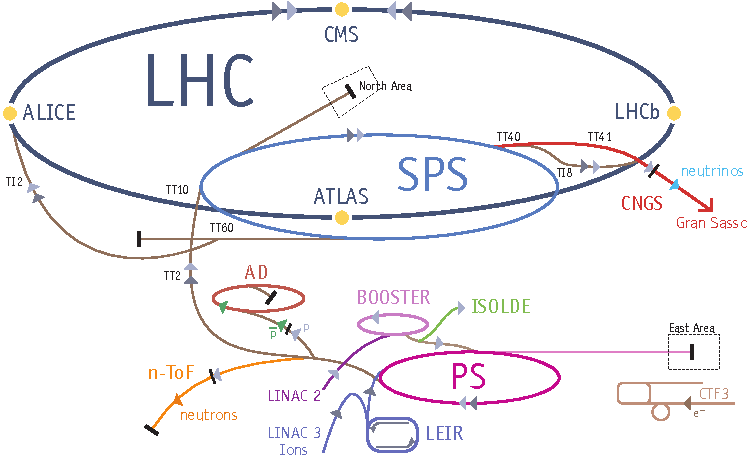
\includegraphics[width=.8\textwidth]{Cernrings}
\end{center}
\begin{minipage}[b]{\textwidth}
\caption{The CERN accelerator complex \cite{cernbro}, which accelerates the protons or ions used in collision experiments through several accelerators with progressively higher energies. The paths protons can take through the machine are marked with light gray triangles. The dark gray triangles mark the paths taken by lead ions when the Collider runs proton--lead or lead--lead collision experiments. Protons are `created' by ionising hydrogen and then injected by \textcolor{Purple}{LINAC 2} into the \textcolor{Plum}{Booster ring}. From there, protons are accelerated by the Proton Synchrotron (\textcolor{Magenta}{PS}) and then the Super Protron Synchrotron (\textcolor{RoyalBlue}{SPS}) before finally being sent into the \textcolor{MidnightBlue}{LHC} ring.}
\label{cernrings}
\end{minipage}
\end{figure}

At a slightly highar level of detail, the LHC is a circular particle accelerator, 27~km in circumference, located in the undergound tunnel under the Cern site in Geneva, and extending into nearby France, dug for the earlier LEP\footnote{\textbf{L}arge \textbf{E}lectron--\textbf{P}roton Collider} Experiment. Within the ring, powerful magnets keep the proton beams confined within the beam pipes, while radiofrequency cavities ensure that the beams achieve and maintain the energy required for the LHC's operation. In 2012, when the data used in this thesis was recorded, that energy was 4~TeV, however the machine was originally designed for 7~TeV beams. The LHC, however, is only the last stage of the even larger machine, which is shown diagrammatically in Fig.~\ref{cernrings}, which accelerates protons from rest to LHC energies. Incidentally, two of the intermediate accelerator rings, the PS and the SPS were once themselves CERN's main colliders.

Although the LHC was designed for proton beams of 7~TeV, which would then collide with a total energy of 14~TeV, a few accidents during commissioning meant that it has not reached that energy yet. The data that will be used in this thesis, which was taken in 2012, was created with 4~TeV beams, for a collision energy of 8~TeV.

\section{The ATLAS detector}
The LHC's two counter-moving proton beams\footnote{Or heavy ion beams, or both, depending on the type of experiments being run during a particular period.} intersect at four points around the LHC ring. The LHC's four detectors are each build around one of these interaction points. The ATLAS detector, along with the CMS\footnote{The \textbf{C}ompact \textbf{M}uon \textbf{S}olenoid.} detector, is a general purpose detector designed to capture as much information as possible about collision events. For this purpose, the ATLAS detector is made up of three concentric layers. From innermost to outermost, these are: the tracking system, the calorimeter system and the muon tracking system. Large magnets are used to apply a magnetic field across the detector, which bends the paths of charged particles. The momentum of such a particle can then be deduced from the radius of the curvature of its track.

\begin{figure}[hbtp]
\begin{minipage}[b]{.69\textwidth}
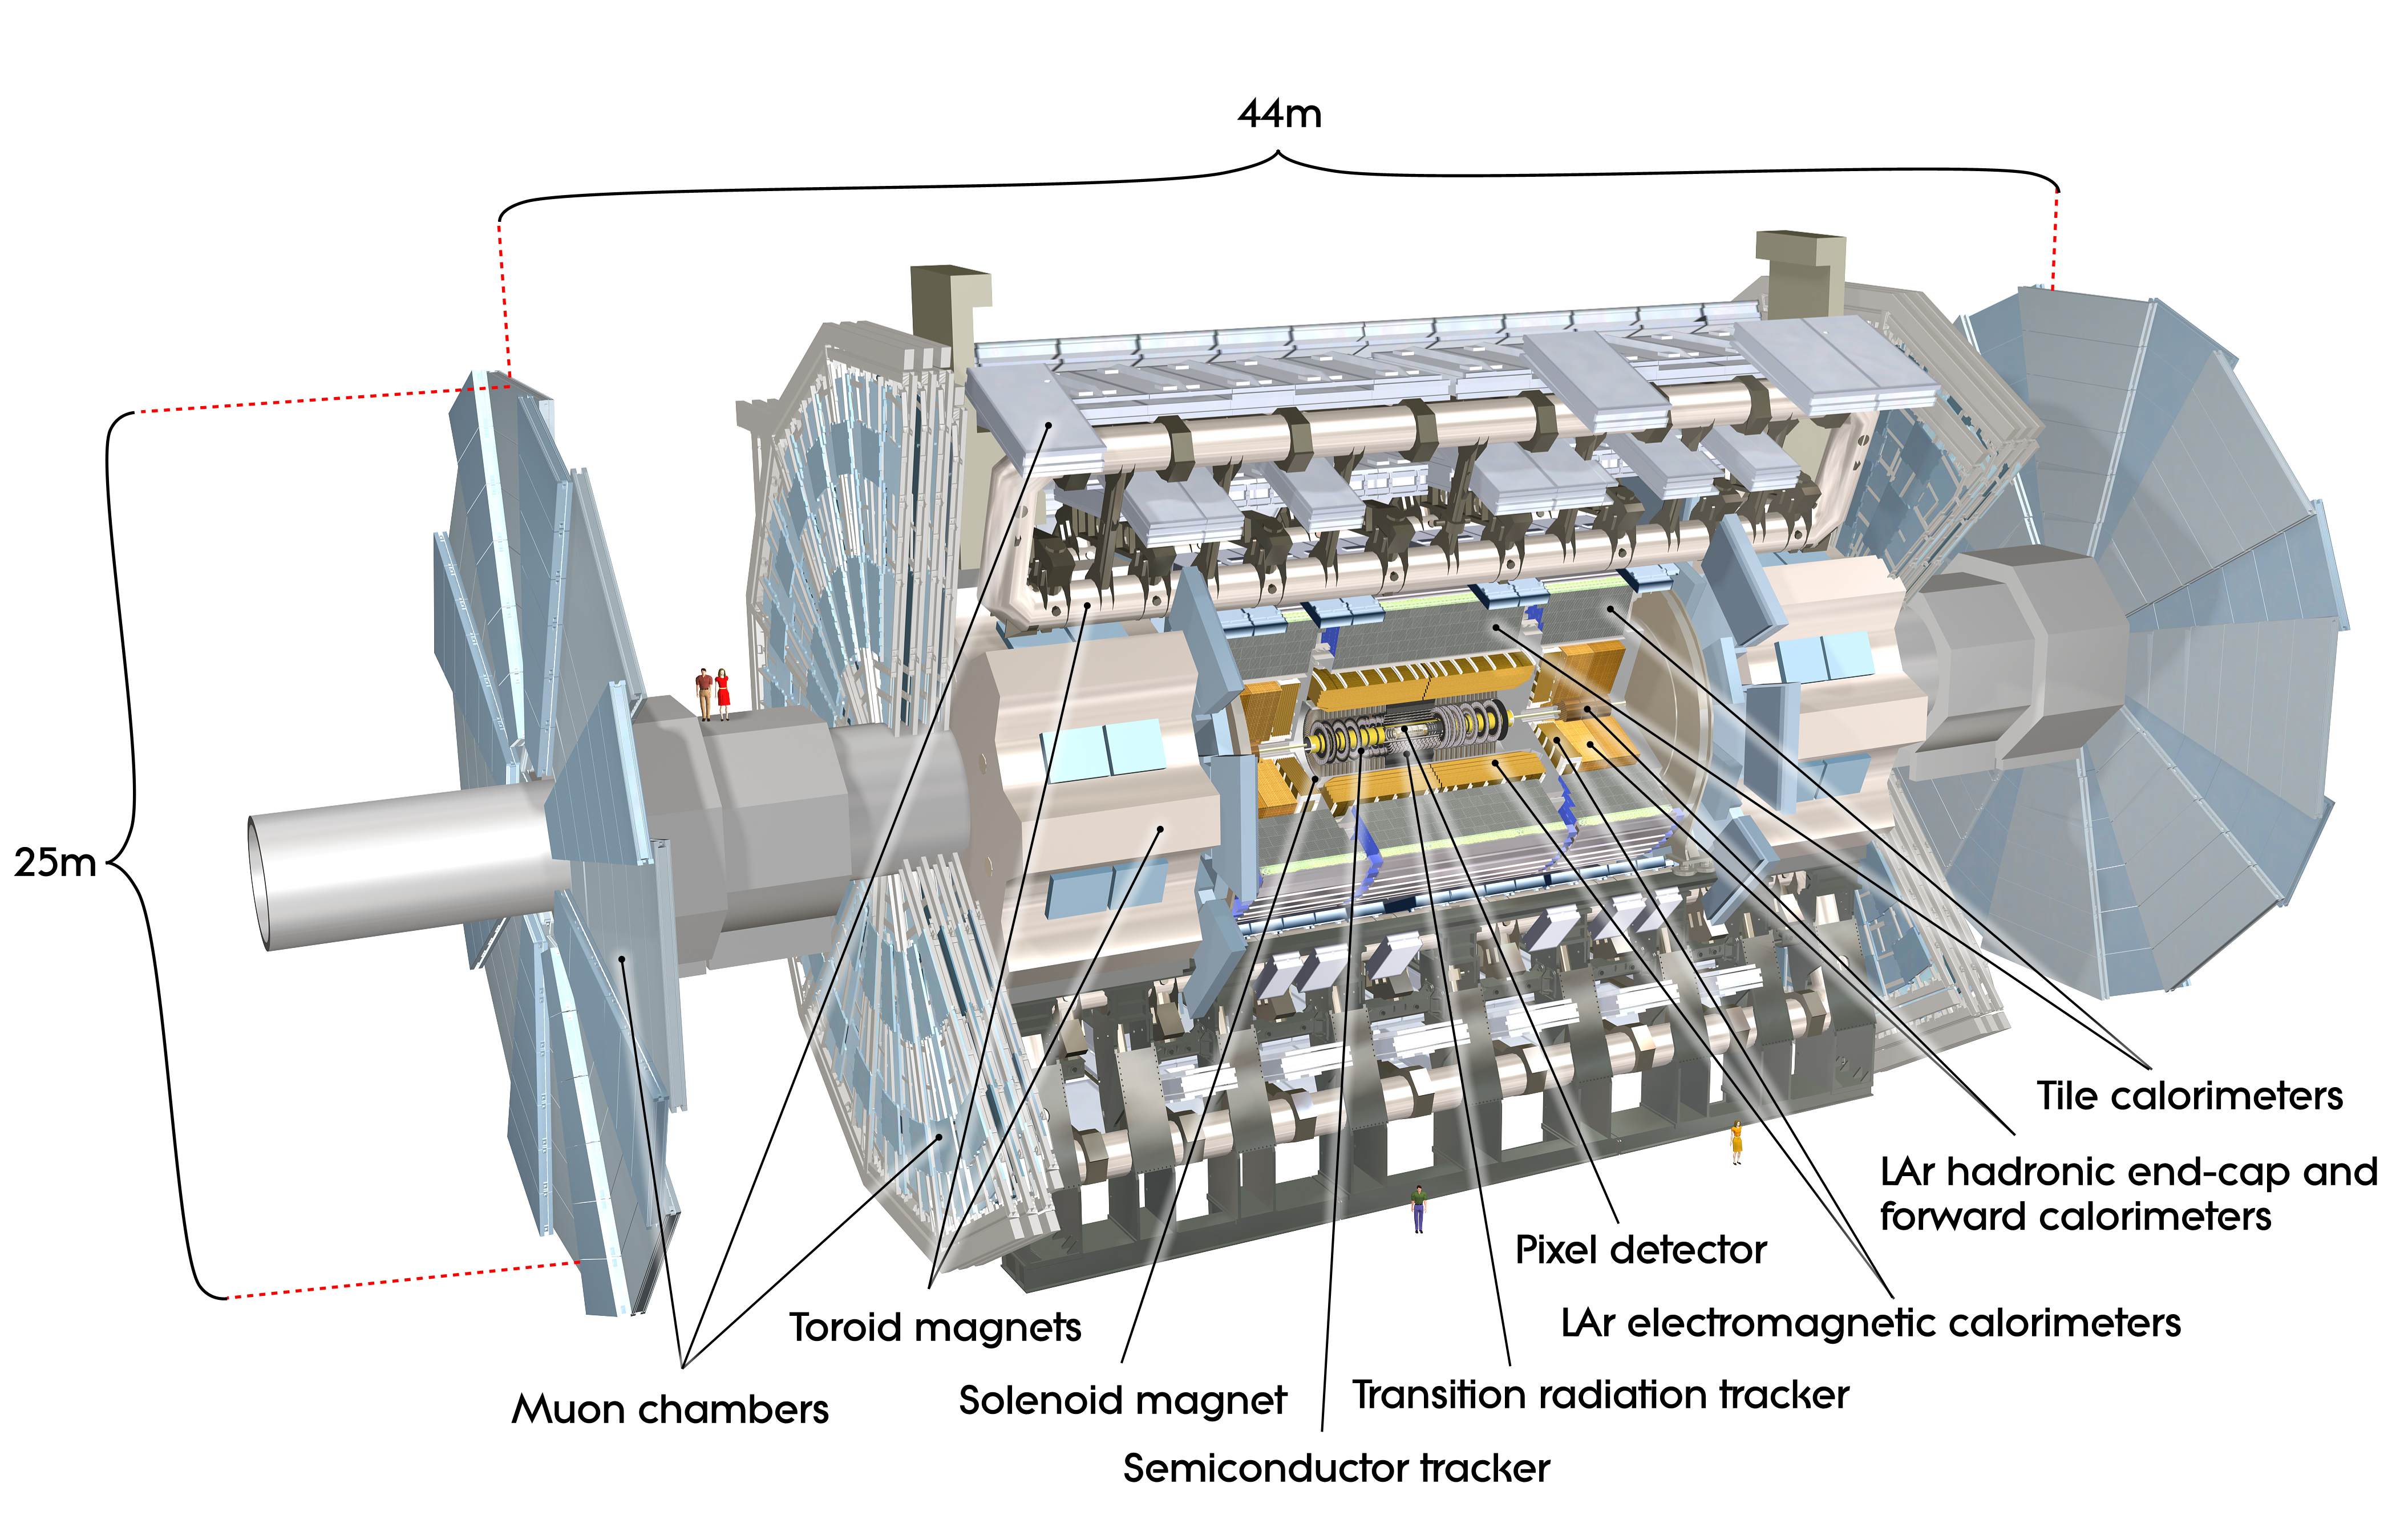
\includegraphics[width=1\textwidth]{AllAtlasBig}
\end{minipage}
\begin{minipage}[b]{.3\textwidth}
\caption{A conceptual sketch of the entire ATLAS detector \cite{atlasweb}. The overall structure is of a layered cylinder centerred on the interaction point. We refer to those parts of the detector that make up the wall of the cylinder as the barrel section, and to the ends of the cylinder as the endcap.}
\end{minipage}
\label{allatlas}
\end{figure}

ATLAS defines its own coordinate system, centred on the interaction point, where the position in the angular direction, perpendicular to the beam pipe, is measured by the coordinate $\phi$ and the angle to the beam pipe is measured in pseudorapidity $\eta$, is defined as
\(\eta=-\ln[\tan(\theta/2)],\)
where $\theta$ is the angle to the beam pipe in radians \cite{green:eta}. The pseudorapidity $\eta$ is a simple transformation of $\theta$, it is 0 at $\theta=\pi/2$, $\infty$ at $\theta=0$ and $-\infty$ at $\theta=\pi$, but is chosen for its similarity to rapidity, $y$, which is additive under Lorenz boosts \cite{green:y}.

The tracking system senses charged particles by the ionisation they leave as they pass through the material of the detector. The innermost layers of the tracking system are made up of semi-conducting chips, which can track particles with a high resolution, but are also expensive, and introduce a lot of mass into the detector. The silicon tracker is further divided into the inner pixel detector and the outer strip detector. The pixel detector can pinpoint a signal very precisely, at the cost of a very large amount of readout data. The pixel detector is responsible for around half of the detector's readout channels. The strip detector works on the same principle, but sacrifices resolution in one direction to more practically conver a larger volume. The outer part of the detector uses drift tubes, which are thin, gas-filled straws with a wire carrying a high voltage strung along its centre line. Gas molecules ionised by a passing charged particle will drift to the wire, where they deposit an electrical signal. The time it takes for a deposited charge to drift to the central wire will depend on the distance between the wire and the particle path. Although there is no way of measuring this time objectively, combining timing information from all the straws in a track helps to narrow down the possible particle path. Because the inner detector is immersed in a magnetic field, charged particles will be deflected, and follow a curved path. By observing the direction and radius of this curvature, we can deduce the sign of the charge and the momentum of a particle.

Excepting the pixel detector, the tracking detectors only tell us that they were passed by a charged particle somewhere along their length. Finding the path of a particle through the tracking detector means fitting a track to the registered hits. Such tracks will usually be expected to begin at the interaction point and end at a deposit in the calorimeter, although detecting b-quarks specifically involves finding vertices slightly removed from the interaction point, and converted photons may begin a track anywhere in the detector. The shape of the detectors means that overlapping tracks and tracks that activate the same detector introduce some potential ambiguity into the process.

Like the tracking system, the calorimeter is divided into two parts: the electromagnetic calorimeter and the hadronic calorimeter. Since the (for the topic of this thesis) crucial photons are most decidedly not hadronic, the EM calorimeter, which is the innermost of the two, will receive a more detailed treatment shortly. However, the purpose of both types of calorimeter is to completely absorb the particles that hit them, and measure the energy they deposit. In ATLAS, all of the calorimeters are sampling calorimeters, which means that layers of absorbing material are sandwiched between layers of sensitive material. As an energetic particle interacts with the absorbing material, it will set off a shower of particles that can be detected in the sensitive layers. The thickness of absorbing material that the sower penetrates will give the energy of the original particle. The barrel section of the hadronic calorimeter is a scintillator calorimeter, meaning that the sensitive layers of the calorimeter is made up of materials that luminesce when exposed to ionising radiation. The absorbing layers of this calorimeter are iron. This type of calorimeter has been chosen as a cost-effective way of covering the large volume that the barrel hadronic calorimeter needs to fill. In the endcap region, the hadronic calorimeters are Liquid Argon (LAr) calorimeters, as are the EM calorimeters, meaning that the sensing material is liquid argon. The absorbing materials in these calorimeters are a combination of iron and lead.

Muons, along with neutrinos, are one of only a few types of particles that can reliably penetrate through both calorimeters although unlike muons, detecting neutrinos directly is something of a hopeless cause. ATLAS' outermost detector system is designed to identify and measure the momentum of muons. Since muons are charged particles, the same types of detector as was used in the inner detector can be used again, but spread out over a much larger volume to compensate for the smaller deflection that a magnetic field of a given strength can impart on muons due to their high mass.

\subsection{The electromagnetic calorimeter}

As the most important tool for detecting photons in ATLAS, the electromagnetic calorimeter deserves a description in slightly greater detail.

\begin{figure}[hbtp]
\begin{minipage}[b]{.59\textwidth}
    \begin{center}
    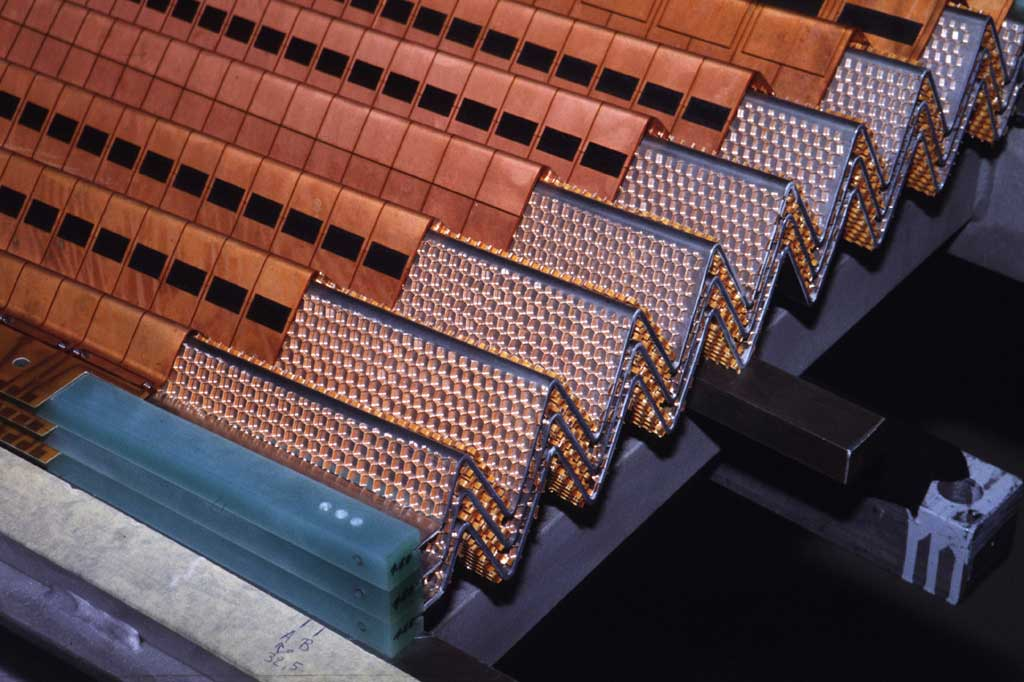
\includegraphics[width=\textwidth]{larpic}
    \end{center}
\end{minipage}
~\begin{minipage}[b]{.4\textwidth}
    \begin{center}
    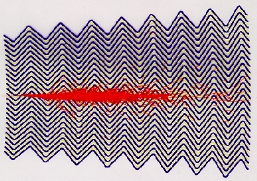
\includegraphics[width=\textwidth]{shower}
    \end{center}
\end{minipage}

\begin{minipage}[t]{.59\textwidth}
    \begin{center}
    \subcaption{A section of the LAr calorimeter.}
    \end{center}
\end{minipage}
~\begin{minipage}[t]{.4\textwidth}
    \begin{center}
    \subcaption{Illustration of a particle shower within the LAr calorimeter. \label{shower}}
    \end{center}
\end{minipage}

\begin{minipage}[b]{.59\textwidth}
    \begin{center}
    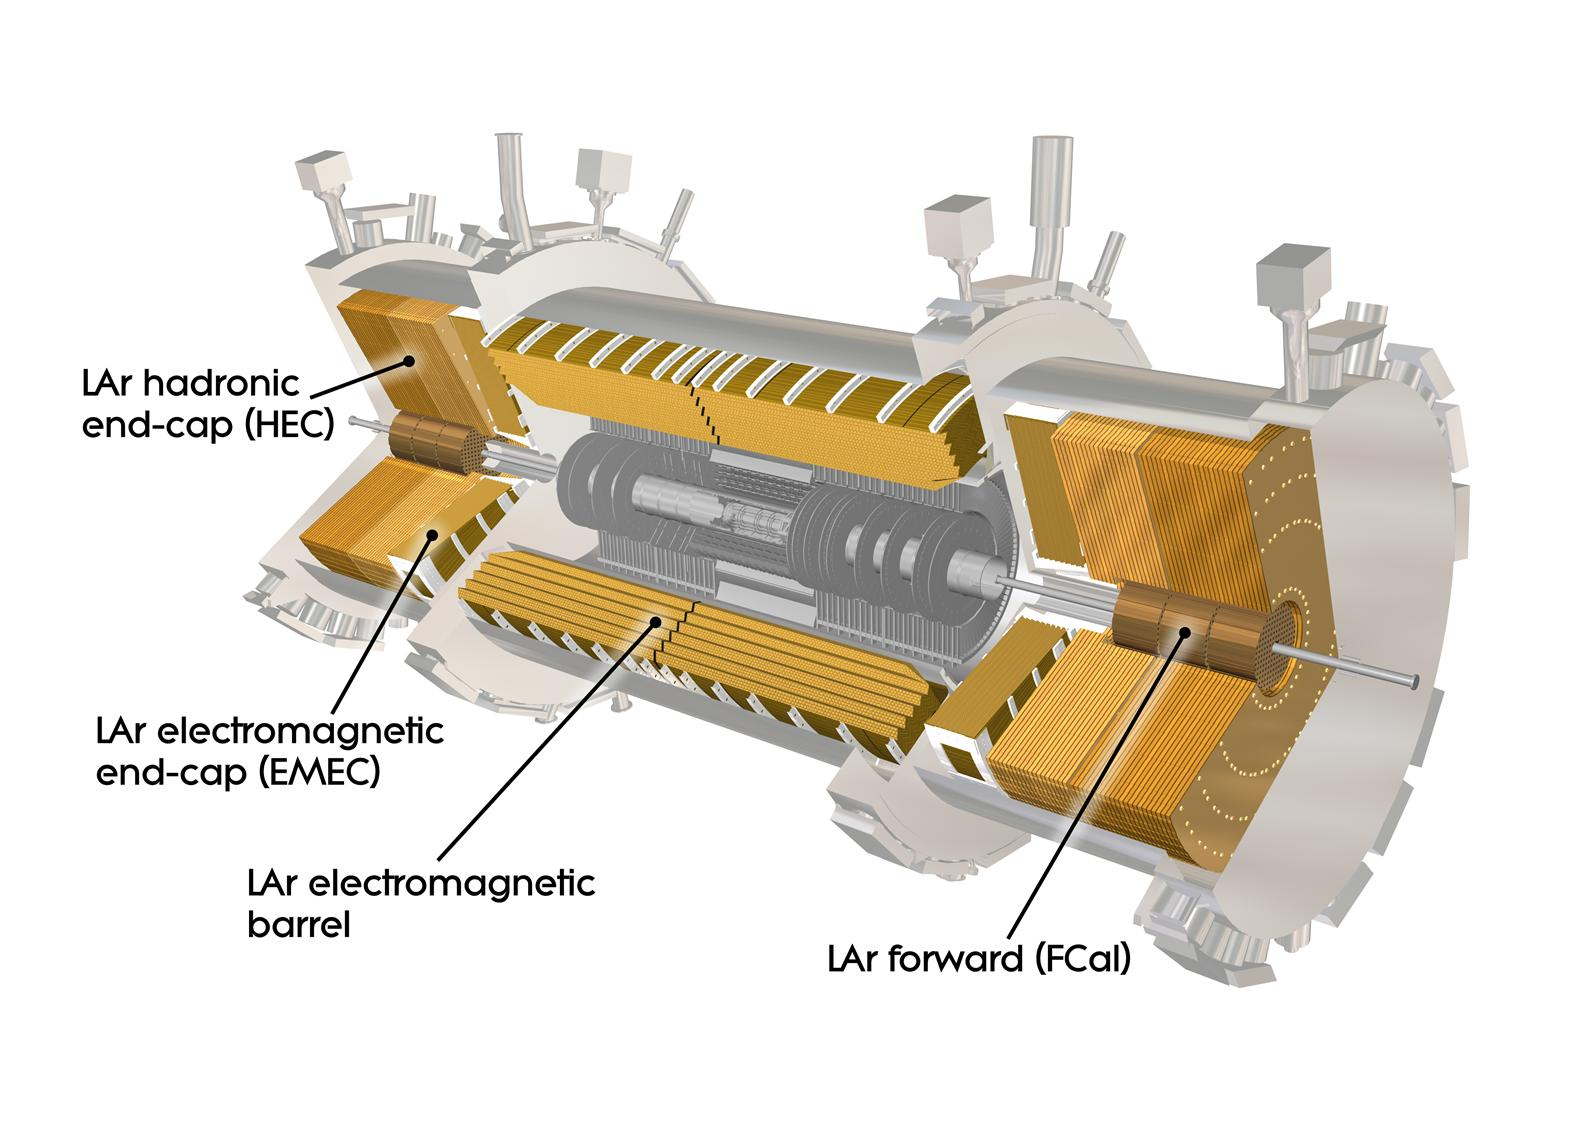
\includegraphics[width=1\textwidth]{emcalover}
    \subcaption{Schematic showing the placement of the LAr calorimeters in ATLAS.}
    \end{center}
\end{minipage}
\begin{minipage}[b]{.4\textwidth}
\caption{Several figures \cite{atlasweb} that illustratie the structure and functioning of the LAr calorimeters. These are sampling calorimeters, which have an absorbing medium (lead or steel) with layers of detecting medium (liquid argon) inserted regularly to keep track of the developing shower shape. In ATLAS, the absorbing medium is made in an accordian shape, visible in (a) and (b), which allows the necessary electronics to be placed on the surface of the absorbing plates, rather than interrupting the calorimeter with non-sensitive signalling pathways.}
\label{calostruc}
\end{minipage}
\end{figure}

The purpose of the EM calorimeter is to attempt to capture those particles that interact electromagnetically and measure their energy. High-energy photons interacting with matter will loose energy almost exclusive through pair production, which converts it into a n electron-positron pair, so long as they have sufficient energy---at least as much as the rest mass of the particles being produced---to do so. Meanwhile, electrons and positrons with high energy moving through matter will loose energy almost exclusively through bremsstrahlung, the loss of kinetic energy by photon emission. Thus, both photons and (anti-)electrons will produce the same sort of signature as they loose energy in the calorimeter, splitting into or emitting new particles, which in turn produce even more particels, in a cascade that expands through the calorimeter, until no more photons with enough energy for pair production can be produced. In the ATLAS calorimeter, this process results in a shower of particles with a shape such as the on illustrated in fig.~\ref{shower}. The depth to which the shower can penetrate an absorbing material will depend on the energy of the initial particle \cite{fernow:sampcal}. The typical distance that a particle has to travel before undergoing one of these processes---the radiation length---are quite similar, and give a natural thickness for the absorption layers of the calorimeter. The active layer, following the same principle as the drift straws in the inner detector, uses a high voltage plate to collect the ionisation charge left in the liquid argon that fills the space between the absorption plates by the passage of high-energy charged particles. The accordian shape of the layers in ATLAS' LAr calorimeters allows the readout electronics to run along their surface, rather than needing to have separate, non-sensitive, channels for them.

Obviously, it is possible for the cascade that the EM calorimeter relies upon to be initiated by any of the material ahead of the calorimeter. To partially account for this possibility, the first sensitive layer, called the presampler, sits in front of the first absorption layer. Photons that convert because of an interaction with material in the inner detector will obviously behave quite differently from unconverted photons, given that it is now an electron-positron pair. Reconstructing these converted photons is a separate task, which we will come back to.

\begin{figure}[hbtp]
\begin{minipage}[b]{.69\textwidth}
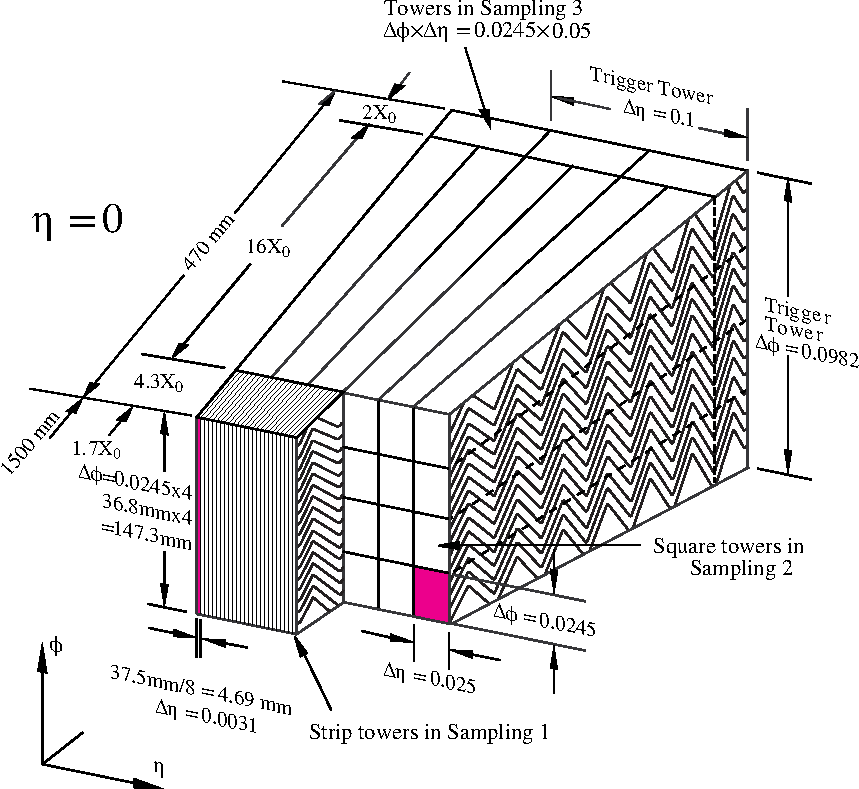
\includegraphics[width=\textwidth]{caldiv}
\end{minipage}
\begin{minipage}[b]{.3\textwidth}
\caption{The division of the EM calorimeter into detecting cells \cite{egede}. The first layer is divided into thin strips for the greatest resolution in the $\eta$ direction, and is sometimes referred to the strip layer. The second layer is divided into roughly square cells, and comprises the bulk of the depth of the detector. The last layer is presumed to only be reached by the very most energetic particles, and can have a coarser division without loosing resolution. This diagram is of the calorimeter at $\eta = 0$, closest to the interaction point. At higher $|\eta|$, the towers angle, so that they are still pointed toward the interaction point.}
\label{caldiv}
\end{minipage}
\end{figure}

The calorimeter is divided into three readout layers, which are split into readout bins as illustrated in fig.~\ref{caldiv}. The first layer is at times referred to as the strip layer, after the narrow bins shaped to achieve the maximum resolution in the $\eta$ direction.

The design of the calorimeter, with some resolution in depth, makes it possible to say something about the shape of the shower as well as the energy deposited. This is useful when different particles may leave differently shaped showers, and makes it possible to say something about the direction from which a particle entered the calorimeter, which is especially useful when dealing with photons, which otherwise leave no way of determining their path in the detector.

\subsection{Photon reconstruction}

Having both the tracker and the calorimeter to show the presence of particles, we can pick out candidates for unconverted photons as those deposits in the EM calorimeter that can not be associated with the end point of one of the tracks found in the tracker. This sample of unconverted photons will doubtless be contaminated with other types of neutral particles, which we will attempt to clean out with subsequent cuts.

Converted photons---photons that undergo pair production because of an interaction with material before the EM calorimeter---will appear in the inner detector as particle tracks that do not extend back to the interaction point. Ideally, the detector would be able to resolve that track of both of the particles created in the photon conversion, in which case it would be able to establish the conversion vertex at their intersection. [However, for a number of reasons, such as the two tracks being too close to one another for the detector to separate, or one of the pair being produced with too low a momentum for the detector to resolve, the detector may not have resolved both particles. This being the case, we must also accept single tracks that do not extend all the way to the interaction point as possible converted photons. This sample too may be contaminated with other types of neutral particles, as well as misidentified electrons.

We can to some extent discriminate between real and impostor photons by looking at the shape shape of the shower in the calorimeter. Since the only information we get from the calorimeter is the magnitude of deposits in each cell, we put together the following shower shape variables from that information to characterise the shape of each shower \cite{Carminati}:

\begin{itemize}
\item $R_\text{had}$, the ratio of energy deposited in the hadronic calorimeter to the cluster energy in the EM calorimeter. Hadronic jets are expected to penetrate deeper into the hadronic calormieter than EM jets.
\item In the middle EM calorimeter layer, we expect non-EM showers to spread wider than electromagnetic ones. The variables that measure the shape of the shower in this layer are
\begin{itemize}
\item $R_\eta$, the ratio in $\eta$ of cell energies in 3 $\times$ 7 versus 7 $\times$ 7 cells.
\item $R_\phi$, the ratio in $\phi$ of cell energies in 3 $\times$ 7 versus 7 $\times$ 7 cells.
\item $w_{\eta 2}$, the width of the shower in the $\eta$ direction in the mid layer.
\end{itemize}
\item The strip layer, with its greater resolution in $\eta$, can pick out some of the internal structure of a jet. Hadron showers tend to show more than one maximum. Variables that measure the shape in the strip layer are
\begin{itemize}
\item $w_{s3}$, the shower width for three strips around the maximum strip.
\item $w_{s\text{ tot}}$, the total lateral shower width in the strip layer.
\item $F_\text{side}$, the faction of energy deposited outside a core of 3 central strips, but within 7 strips.
\item $\Delta E$, the difference in energy of the strip with the second largest energy deposited and the strip with the smallest energy deposited between the two leading strips.
\item $E_\text{ratio}$, the ratio of the energy difference associated with the
largest and second largest energy deposits over the
sum of these energies.
\end{itemize}
\end{itemize}

The cuts made in these variables vary with $\eta$, and separate cuts exist for converted and unconverted photons. For the exact values used, see \cite{Carminati}. The cuts in $R_\text{had}$, $R_\eta$ and $w_{\eta2}$ collectively from the loose selection criteria, while the combination of all the cuts forms the tight selection criteria. These selections will become important later in the analysis. More immediately, though, they will allow us to record photon events in the first place.

\subsection{Triggering and data collection}
When in full operation, the LHC will deliver a bunch crossing in ATLAS' interaction point every 50~ns. Reading out the whole detector produces 1.6~MB of information, which, if the detector was to be read out completely with every crossing, would produce a data rate of 32~TB/s.\footnote{For perspective, that is approximately equal to the estimated global IP traffic rate in 2015, according to \cite{wolframip}.} Clearly, recording every collision is impossible. To trim down that data quantity, the detector uses a system that examines every collision for potentially interesting events, and triggers event recording if it finds one. In ATLAS, this trigger system has three levels \cite{detectorpaper}.

The level-1 trigger, which must perform selection at the same cadence as the collision events occur, runs on specialised hardware built into the calorimeter and muon systems, and evaluates the worthiness of an event based solely on the information available to them locally. As an example, the level-1 trigger used to select data for this thesis, called \texttt{2g40\_loose}, requires that the EM calorimeter has recorded at least two deposits of 40 GeV transverse energy, which fulfils the loose shower shape cuts. These hardware triggers reduce the event frequency from 20 MHz to 100 kHz.

The level-2 trigger has access to full precision data from all parts of the detector, and runs on a dedicated computing cluster close to the detector. It combines information from all parts of the detector to better determine if the deposits identified by the level-1 trigger are actually interesting events. Staying with photon candidates in the EM calorimeter, this trigger might use information from the hadronic calorimeter to separate out hadronic jets, or tracking information from the inner detector to distinguish between neutral and charged particles. This trigger reduces the data rate to below 10 kHz.

The level-3 trigger---or the event filter---looks at fully reconstructed events and calculated and derived physical properties, such as transverse momentum, which allows it to cut in those quantities to further refine the event selection. This trigger brings the data rate down to the final rate of around 300 Hz on average. The output rate varies, since the rates with which interesting events occur are purely random, and the final data rate can peak up to 600 Hz for short periods.

Unfortunately, there is no direct relationship between the frequency of an event type, and how interesting that event type is to analyses. For this reason, some triggers that produce more output than we are interested\footnote{Detailing how the level of interest in a particular event type is defined quickly strays into the area of ATLAS internal politics, which are most definitely beyond the scope of this thesis.} in keeping are prescaled, so that only some predetermined fraction of events that pass are stored. Since diphoton events are important to the Higgs search, the trigger used to gather the data used in this analysis has been left unprescaled.

It turns out that there is a good amount of overlap in the derived quantities that different analyses will need to calculate from the data that is stored by the trigger system. For this reason, the ATLAS collaboration encompasses several working groups that generate datasets that cointain these shared quantities, and make then available to the analyses that need them. For the present analysis, we will use the \texttt{NTUP\_PHOTON} container, which the E/gamma working group is responsible for.


\chapter{Data}
The ATLAS data that will be used for this thesis was taken in 2012, during the 8~TeV run of the LHC, during which ATLAS recorded 20.3~fb$^{1}$ of integrated luminosity.

\begin{figure}[hbt]
\begin{minipage}[b]{.69\textwidth}
\hspace{-1em}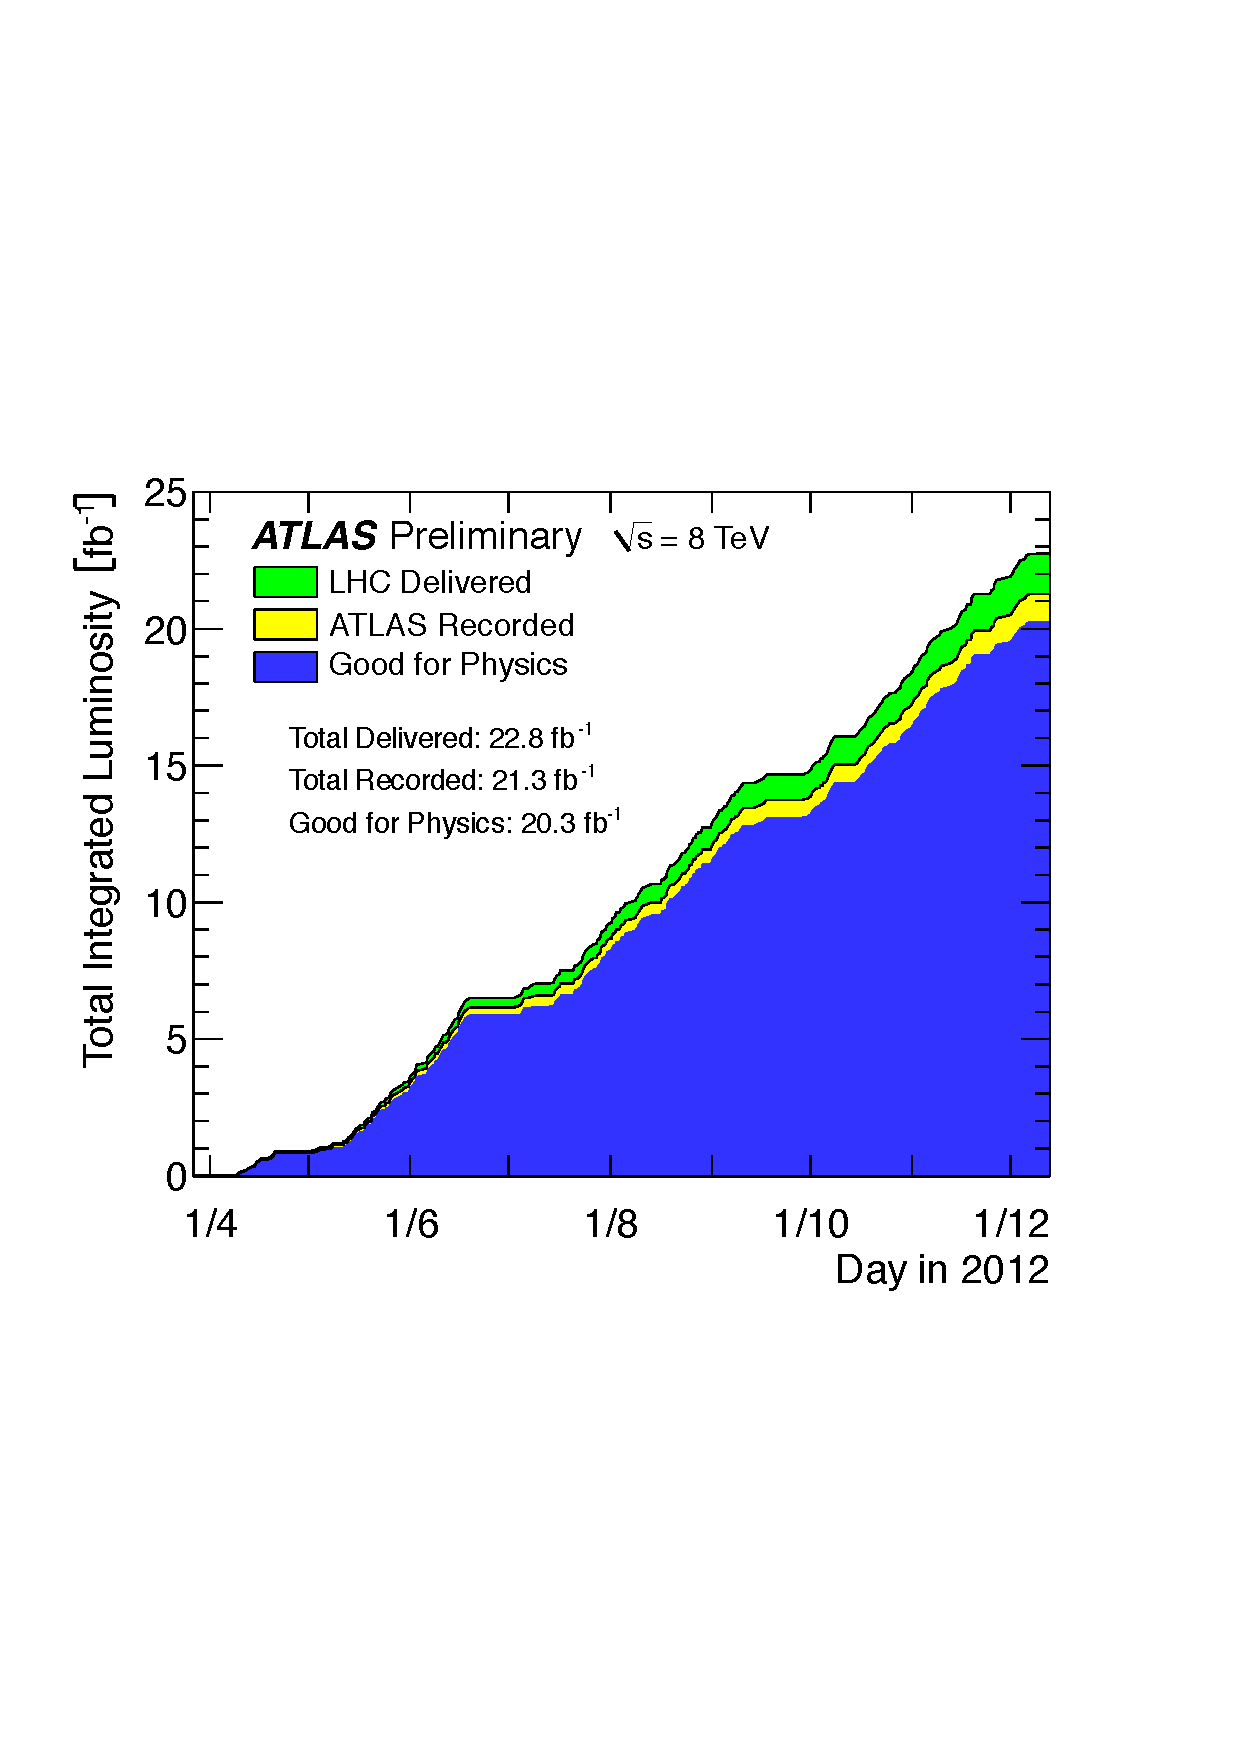
\includegraphics[width=\textwidth]{figures/intlumi}
\end{minipage}\hfill\begin{minipage}[b]{.3\textwidth}
\caption{A plot showing the integrated luminosity delivered by the LHC (green), recorded by ATLAS (yellow), and passing data quality cuts (blue), over the course of the 8 TeV run in 2012 \cite{publiclumi}.
\label{intlumi}}
\end{minipage}
\end{figure}

Something, something, photon container, skim etc. etc. 18301.3~nb$^{-1}$.

A significant fraction of this data will be made up of events that are not relevant to the present analysis, so to reduce the data set to a managable size, the unneeded events are skimmed away.

\section{Skimming}


\chapter{Analysis}
All of the bits so far are put together, and a limit on the size of
$\Lambda$ is found.

\chapter{Conclusion}
The found limit is re-iterated, and the caveats on its prescisioin are
listed. Implications are gone through, and proposals for improvements
are made.

\renewcommand{\bibname}{References}
\bibliographystyle{plainurl}
\bibliography{cite}

\end{english}
\end{document}
